\documentclass[a4paper,11pt]{book}
%\textwidth 11,8 cm
%\textheight 17 cm
\textheight 23 cm
\usepackage[dvipdfmx]{graphicx} \usepackage{bmpsize}  %\usepackage{graphicx}
\usepackage{amsmath}
\usepackage{amsfonts}
\usepackage{amssymb}
\usepackage{stmaryrd}
\usepackage{makeidx}
\usepackage{times}
\usepackage{hevea}
%\usepackage{mathptmx}
%Uncomment next line for pdflatex and use includegraphics with eps file
% for latex2html don't use the option [width=\textwidth]
% check that xfig files are exported magnif 100%
%\usepackage[francais]{babel}
\usepackage{ifpdf}
\ifpdf
 \usepackage[pdftex,colorlinks]{hyperref}
\else
 \usepackage[ps2pdf,breaklinks=true,colorlinks=true,linkcolor=red,citecolor=green]{hyperref}
 \usepackage{pst-plot}
\fi

%\def\@evenhead{\thepage\hfill{\footnotesize\textit{\leftmark}}}
%\def\@oddhead{\footnotesize{\textit{\rightmark}}\hfill\thepage}
%\usepackage{hp}
\usepackage[utf8]{inputenc}
\usepackage[T1]{fontenc}
%\usepackage[francais]{babel}
\usepackage{latexsym}

% Inline commands; use \texttt
% Displayed commands and output, use this

% For graphics
\newcommand{\includeimage}[1]
{\includegraphics[width=0.75\textwidth]{#1}} 

\newcommand{\R}{{\mathbb{R}}}
\newcommand{\C}{{\mathbb{C}}}
\newcommand{\Z}{{\mathbb{Z}}}
\newcommand{\N}{{\mathbb{N}}}

%\usepackage[pdftex]{hyperref}
\title {Symbolic algebra and Mathematics with {\tt Xcas}}
\author{Ren\'ee De Graeve, Bernard Parisse\footnote{Universit\'e de Grenoble, initial translation of parts of the French user manual},\\ 
Jay Belanger\footnote{Full translation and improvements}\\
Sections written by Luka Marohnić\footnote{Optimization, signal processing. The graph theory is in a separate manual.}}
\date{}
\makeindex
\usepackage{cutting}
\begin{document}
\newcommand{\asinh}{\,\,\mbox{asinh\,}}
\newcommand{\atanh}{\,\,\mbox{atanh\,}}
\maketitle
% {\bf \centerline{Remerciements}}

% \vspace{1cm}

% Je  remercie:
%  \begin{itemize}
% \item Bernard Parisse for ses pr\'ecieux conseils andses remarques sur ce texte,

%  \end{itemize}

\vfill


\copyright\ 2002, 2007 Ren\'ee De Graeve, Bernard Parisse\\
\verb|renee.degraeve@wanadoo.fr|\\
\verb|bernard.parisse@ujf-grenoble.fr|\\



\newpage
\tableofcontents

\chapter{Index}
\printindex

\chapter{Introduction}

\section{Notations used in this manual}

In this manual, the information that you enter will be typeset in
typewriter font.  User input typically takes one of three forms:
\begin{itemize}
\item Commands that you enter on the command line.\\
For example, to compute the sin of $\pi/4$, you can type
\begin{center}
{\tt sin(pi/4)}
\end{center}

\item Commands requiring a prefix key.\\
These will be indicated by separating
the prefix key and the standard key with a plus \texttt{+}.  For
example, to exit an \texttt{Xcas} session, you can type the control
key along with the \texttt{q} key, which will be denoted
\begin{center}
{\tt  Ctrl+Q}
\end{center}

\item Menu commands.\\
When denoting menu items, submenus will be connected using
$\blacktriangleright$.  For example, from within \texttt{Xcas} you
can choose the \texttt{File} menu, then choose the \texttt{Open}
submenu, and then choose the \texttt{File} item.  This will be
indicated by
\begin{center}
  {\tt File $\blacktriangleright$ Open $\blacktriangleright$ File}
\end{center}
\end{itemize}

The index will use different typefaces for different parts of
the language.  The commands themselves will be written with normal
characters, command options will be written in italics and values of
commands or options will be written in typewriter font.   For example
(as you will see later), you can draw a blue parabola with the command
\begin{center}
  {\tt plotfunc(x\^{}2,color = blue)}
\end{center}
In the index, you will see
\begin{itemize}
\item
  plotfunc, the command, written in normal text.
\item
  \textit{color}, the command option, written in italics.
\item
  \texttt{blue}, the value given to the option, written in typewriter
  font.
\end{itemize}

\section{Interfaces for the \texttt{giac} library}

The \texttt{giac} library is a C++ mathematics library.  
It comes with two interfaces for users to use it directly; a graphical
interface and a command-line interface.

The graphical interface is called \texttt{Xcas}, and is the most
full-featured interface.  As well being able to do symbolic and numeric
calculations, it has its own programming language, it can draw graphs,
it has a built-in spreadsheet, it can do dynamic geometry
and turtle graphics.

The command-line interface can be run inside a terminal.  It can also
do symbolic and numeric calculations and works with the programming
language.  In a graphical environment, the command-line interface can
also be used to draw graphs.

There is also a web version, which can be run through a browser,
either over the internet or from local files.  Other programs (for
example, \texttt{TeXmacs}) have interfaces for the command-line
version.

\subsection{The \texttt{Xcas} interface}

How you run \texttt{Xcas} in a graphical environment depends on which
operating system you are using.
\begin{itemize}
  \item
If you are using Unix, you can usually find
an entry for the program in a menu provided by the environment.
Otherwise, you can start it from a terminal by typing
\begin{center}
  {\tt xcas \&}
\end{center}
If for some reason \texttt{Xcas} becomes unresponsive, you can open a
terminal and type
\begin{center}
  {\tt killall xcas}
\end{center}
That will kill any running \texttt{Xcas} processes.  When you restart
\texttt{Xcas}, you will be asked if you want to resume where you left
off using an automatic backup file.
\item
If you are running Windows, you can use the explorer to go to the
directory where \texttt{Xcas} is installed.  In that directory will be
a file called \texttt{xcas.bat}.  Clicking on that file will start
\texttt{Xcas}.
\item
If you are running Mac OS, you can use the Finder to go to the
\texttt{xcas\_image.dmg} file and double-click it.  Then double-click
the \texttt{Xcas} disk icon.  Finally, to launch \texttt{Xcas},
double-click the \texttt{Xcas} program.
\end{itemize}
When you start \texttt{Xcas}, a
window will pop up with menu entries across the top, a bar
indicating information about the current \texttt{Xcas} configuration,
and an entry line you can use to enter commands.  This interface will
be described in more detail later, and you can get help
from within \texttt{Xcas} with the menu item
\begin{center}
\texttt{Help$\blacktriangleright$Interface}
\end{center}

\subsection{The command-line interface}

In Unix and MacOS you can run \texttt{giac} from a terminal with
the command \texttt{icas} (the command \texttt{giac} also works).
There are two ways to use the command-line interface.

If you just want to evaluate one expression, you can give
\texttt{icas} the expression (in quotes) as a command line argument.
For example, to factor the polynomial $x^2-1$, you can type
\begin{center}
  {\tt icas 'factor(x\^{}2-1)'}
\end{center}
at a command prompt.  The result will be
\begin{center}
  {\tt (x-1)*(x+1)}
\end{center}
and you will be returned to the operating system command line.

If you want to evaluate several commands, you can enter an interactive
\texttt{giac} session by entering the command
\texttt{icas} (or \texttt{giac}) by itself at a command prompt.  You
will then be given a prompt specifically for \texttt{giac} commands,
which will look like
\begin{verbatim}
  0>>
\end{verbatim}
You can enter a giac command at this prompt and get the result.
\begin{verbatim}
 0>> factor(x^2-1)
 (x-1)*(x+1)
 1>>
\end{verbatim}
After the result, you will be given another prompt for \texttt{giac}
commands.  You can exit this interactive session by typing
\texttt{Ctrl+D}.

You can also run \texttt{icas} in batch mode; that is, 
you can have \texttt{icas} run \texttt{giac} commands stored in a
file.  This can be done in Windows as well as Unix and Mac OS.
To do this, simply enter 
\begin{verbatim}
  icas filename
\end{verbatim}
at a command prompt, where \textit{filename} is the name of the file
containing the \texttt{giac} commands.

\subsection{The Firefox interface}

You can run \texttt{giac} without installing it by using a
javascript-enabled web browser.  Using Firefox for this is highly
recommended; Firefox will run \texttt{giac} several times faster than
Chrome, for example, and Firefox also supports MathML natively.

%This version won't have as much functionality as \texttt{Xcas}, but it
%doesn't require any software beyond a web browser to be installed.

To run \texttt{giac} through Firefox, you can open the url
\url{https://www-fourier.ujf-grenoble.fr/~parisse/giac/xcasen.html}.
At the top of this page is a button which will open a quick tutorial;
the tutorial will also tell you how to install the necessary files to
run \texttt{giac} through Firefox without being connected to the
internet.

\subsection{The TeXmacs interface}

TeXmacs (\url{http://www.texmacs.org}) is a sophisticated word
processor with special mathematical features.  As well as being
designed to nicely typeset mathematics, it can be used as a frontend
for various mathematics programs, such as \texttt{giac}.

Once you've started TeXmacs, you can interactively run \texttt{giac}
within TeXmacs with the menu command
\texttt{Insert$\blacktriangleright$Session$\blacktriangleright$Giac}.
Once started, you can enter \texttt{giac} commands as you would in the
command-line interface.  The TeXmacs interface will also have a menu
specifically for \texttt{giac} commands.

Within TeXmacs, you can combine \texttt{giac} commands and output with
ordinary text.  To enter normal text within a \texttt{giac} session,
use the menu item \texttt{Focus$\blacktriangleright$Insert Text Field
Above}.  You can reenter a \texttt{giac} entry line by clicking on it
with a mouse.

\subsection{Checking the version of \texttt{giac} that you are using:
\texttt{version, giac}}
\index{version}
\index{giac}

The \texttt{version} (or \texttt{giac}) command returns the version of \texttt{giac} that
is running.\\
Input:
\begin{center}
  \tt
  version()
\end{center}
Output:
\begin{center}
  \tt
  "giac 1.5.0, (c) B. Parisse and R. De Graeve, Institut Fourier, Universite de Grenoble I"
\end{center}

% \subsection{The Emacs interface}

% You can run a \texttt{giac} session using \texttt{mupacs}
% (\url{http://mupacs.sourceforge.net}), an Emacs mode for MuPAD, a
% computer algebra system no longer independently available.  Since this
% mode was created for MuPAD, you 

\chapter{The \texttt{Xcas} interface}

\section{The entry levels}

The \texttt{Xcas} interface can run several independent calculation
sessions, each session will be contained in a separate tab.  Before
you understand the \texttt{Xcas} interface, it would help to be
familiar with the components of a session.

Each session can have any number of input levels.  Each input level
will have a number to the left of it; the number is used to identify
the input level.  Each level can have one of the following:
\begin{itemize}
  \item A command line.\\
  This is the default; you can open a new
  command line with \texttt{Alt+N}.\\
  You can enter a \texttt{giac} command (or a series of commands
  separated by semicolons) on a command line and send it to be
  evaluated by hitting enter.  You can also scroll through the command
  history with \texttt{Shift+Up} and \texttt{Shift+Down}.
  
  If the output is a number or an expression, then it will appear in
  blue text in a small area below the input region; this area is an
  expression editor.  There will be a scrollbar and a small \texttt{M}
  to the right of this area; the \texttt{M} is a menu which gives you
  various options.

  If the output is a graphic, then it will appear in a graphing area
  below the input region.  To the right of the graphic will be a
  control panel allowing you to manipulate the graphic.

  \item  An expression editor.\\  
  You can open an expression editor with
  \texttt{Alt+E}.
  
  \item A two-dimensional geometry screen.\\
  You can open up such a
  screen with \texttt{Alt+G}.
  This level will have a screen, as well as a control panel, menus and a
  command line to control the screen.
  
  \item A three-dimensional geometry screen.\\
  You can open up such a
  screen with \texttt{Alt+H}.
  This level will have a screen, as well as a control panel, menus and
  a command line to control the screen.
  
  \item A turtle graphics screen.\\
  You can open up such a screen with
  \texttt{Alt+D}.
  This level will have a screen, as well as a program editor and
  command line.
  
  \item A spreadsheet.\\
  You can open up a spreadsheet with \texttt{Alt+T}.
  A spreadsheet will be able to open a graphic screen.
  
  \item A program editor.\\
  You can open up a program editor with
  \texttt{Alt+P}.
  
  \item A comment line.  You can open up a comment line with
  \texttt{Alt+C}.
\end{itemize}
Using commands discussed later, different types of levels can be
combined to form a single hybrid level.  Levels can also be moved up
or down in a session, or even moved to a different session.

The level containing the cursor is the \emph{current level}.  The
current level can be evaluated or re-evaluated by typing enter.

A level can be selected (for later operations) by clicking on the
number in the white box to the left of the level.  Once selected, the
box containing the number will turn black.  You can select a range of
levels by clicking on the number for the beginning level, and then
holding the shift key while you click on the number for the ending level.

You can copy the instructions in a range of levels by selecting the
range, and then clicking the middle mouse button on the number of the
target level.

\section{The starting window}

When you first start \texttt{Xcas}, you will be given a largely blank window.
\begin{center}
  \includeimage{xcas-open.png}
\end{center}
The first row will be the main menus; you can 
save and load \texttt{Xcas} sessions, configure \texttt{Xcas} and its
interface and run various commands with entries from these menus.

The second row will be tabs; one tab for each session that you are
running in \texttt{Xcas}.  The tabs will contain the name of the
sessions, or \texttt{Unnamed} if a session has no name.  The first
time you start \texttt{Xcas}, there will be only one unnamed session.

The third row will contain various buttons.
\begin{itemize}
  \item The first button, \framebox{\tt ?}, will open the help index.
  (The same as the \texttt{Help$\blacktriangleright$Index} menu entry.)
  If there is a command on the command line, the help index 
  (see \ahrefloc{helpindex}{help index}
  \begin{latexonly},p.\pageref{sssec:helpind}\end{latexonly})
  will open at this command.
  
  \item The second button \framebox{\tt Save}, will save the session
  in a file.  The first time you click on it, you will be prompted for
  a file name ending in \texttt{.xws} to save the session in.  The
  button will be pink if the session is not saved or if it has changed
  since the last change, it will be green once the session is saved.
  The name in the title will be the name of the file used to save the
  session.

\item The third button, which in the picture above is\\
  \framebox{\tt Config : exact real RAD 12 xcas 6.2148M}, is a status
  line indicating the current \texttt{Xcas} configuration. 
  (See section \ref{sec:config}.)
  If the session is unsaved, it will begin with \texttt{Config :}; if the
  session is saved in a file \textit{filename.xws}, this button will
  begin with \texttt{\texttt{Config }\textit{filename.xws}\texttt{ :}}.
  Other information on this status line:
  \begin{itemize}
    \item \texttt{exact} or \texttt{approx}.  
    (See subsection \ref{ssec:approx}.)
    This tells you whether
    \texttt{Xcas} will give you exact values, such as
    $\sqrt{2}$, when possible or to give you decimal approximations.

    \item \texttt{real}, \texttt{cplx} or \texttt{CPLX}.  
    (See subsections \ref{ssec:complex} and \ref{ssec:cvars}.)
    When this shows \texttt{real}, then (for example) \texttt{Xcas} will by
    default only find real solutions of equations.  When this shows
    \texttt{cplx}, the \texttt{Xcas} will find complex solutions of
    equations.  When this shows \texttt{CPLX}, then \texttt{Xcas} will
    regard variables as complex; for example, it won't simplify
    \texttt{re(z)} (the real part of the variable $z$) to \texttt{z}.

    \item \texttt{RAD} or \texttt{DEG}.  
    (See subsection \ref{ssec:angles}.)
    This tells you whether
    angles, as in trigonometric arguments, are measured in radians
    or degrees.

    \item An integer.  (See subsection \ref{ssec:sigdig}, indicating
    how many significant digits will be used in floating point calculations.

    \item \texttt{xcas}, \texttt{maple}, \texttt{mupad} or \texttt{ti89}.
    (See subsection \ref{ssec:lang}.) This tells you what syntax
    \texttt{Xcas} will use.  \texttt{Xcas} can be set to emulate the
    languages of Maple, MuPAD or the TI89 series of calculators.

    \item The last item indicates how much memory \texttt{Xcas} is using.
  \end{itemize}
  Clicking on this status line button will open a window where
  you can configure the settings shown on this line as well as some
  other settings; you can do the same with the menu item
  \texttt{Cfg$\blacktriangleright$CAS Configuration}.
  (See subsection \ref{ssec:confcomp}.)      

  \item The fourth button, \framebox{\tt STOP} (in red), can be used
  to halt a computation which is running on too long.

  \item The fifth button, \framebox{\tt Kbd}, can be used to toggle an
  on-screen scientific keyboard at the bottom of the window.
  \begin{center}
    \includeimage{xcas-scientific-keyboard.png}
  \end{center}
  Along the right hand side of the keyboard are some keys that can
  be used to change the keyboard.  
  \begin{itemize}
    \item The \texttt{X} key will hide the
    keyboard, just like pressing the \framebox{\tt Kbd} button again.

    \item The \texttt{cmds} key will toggle a menu bar at the bottom of the
    screen which can be used as an alternate menu or persistent
    submenu.  This bar will contain buttons, \texttt{home},
    \texttt{<{}<}, some menu titles, \texttt{>{}>}, \texttt{var},
    \texttt{cust} and \texttt{X}.

    The \texttt{<{}<} and \texttt{>{}>} buttons will scroll through menu
    items.  Clicking on one of the menu buttons will perform the appropriate
    action or replace the menu items by submenu items.  When submenu
    items appear, there will also be a \texttt{BACK} button to return to
    the previous menu.  Clicking on the \texttt{home} button returns the
    menu buttons to the main menu.  
  
    After the menu buttons is a \texttt{var} button.  This will replace
    the menu buttons by buttons representing the variables that you have
    defined.  After that is a \texttt{cust} button, which will display
    commands that you store in a list variable \texttt{CST} (see section
    \ref{ssec:CST}).
  
    The last button, \texttt{X}, will close the menu bar.

    \item The \texttt{msg} key will bring up a message window at the bottom
    of the window which will give you helpful messages; for example, if
    you save a graphic, it will tell you the name of the file it is
    saved in and how to include it in a \LaTeX{} file.  

    \item The \texttt{abc} key will toggle the keyboard between the
    scientific keyboard and an alphabetic keyboard.
  \end{itemize}

  \item The fifth button, \framebox{\tt X}, will close the current
  session.
\end{itemize}

\section{Getting help}

\texttt{Xcas} is an extensive program, but you can get help in several
different ways.  The help menu (see section \ref{ssec:helpmenu}) has
several submenus for various forms of help, some of which are
mentioned below.

\subsubsection{Tooltips}

If you hover the mouse cursor over certain parts of the \texttt{Xcas}
window, a temporary window will appear with information about the
part.  For example, if you move the mouse cursor over the status line,
you will get a message saying \texttt{Current CAS status.  Click to
modify.}

If you type a function name into the \texttt{Xcas} command line, a
similar temporary window will appear with information about the
function. 

\subsubsection{HTML help}

If you hit the \texttt{F12} button, you will be given a window in
which you can use to search the html version of the manual.  If you
type a string in the search area, you will be given a list of help
topics that contain the string.  If you choose a topic and click
\texttt{View}, your web browser will show the appropriate page of 
the manual.

You can also get HTML help with the menu entry
\texttt{Help$\blacktriangleright$Find word in HTML help}.

\subsubsection{The help index}
\label{sssec:helpind}\aname{helpindex}{}


If you click on the \framebox{?} button on the status line you will
get the help index.

The help index is a list of the \texttt{giac} function and variable
names.  Along with the list, the help index window has an area listing
words related to any chosen word and words synonymous to the chosen word.

You can scroll through the help index items and click on the word that
you want.  There is also a line in the help index window that you can
use to search the index; you can enter some text and be taken to the
part of the index with words beginning with that text.  The \texttt{?}
button next to this search line will open the HTML help window.

Below the search line, there is an area which will have a description
of the chosen command, and below that is an area which will have
examples of the command being used.  If the command is a function,
then between the description and examples will be some boxes in which
you can enter arguments for the command.  Filling in these boxes and
hitting enter will put the function on the command line.

At the top of the help index window is a \texttt{Details} button.  If
you click on that, a web page will open up in your browser with the
relevant portion of the manual. If you click on the
\framebox{\texttt{?}} next to the search line, you will be taken to
the HTML help window.

Besides clicking on the \framebox{\texttt{?}} on the status line,
there are other ways to get to the help index.
\begin{itemize}
  \item
  You can get to the help index by using the menu item 
  \texttt{Help$\blacktriangleright$Index}.  
  
  \item 
  You can press the tab button while at the \texttt{Xcas} 
  command line to get to the help index.  If you have
  entered part of a command name, you will be at the part of the index
  with words beginning with the text that you entered.
  
  \item
  If you select a command from the menu, then as well as putting the
  command on the command line, you will be taken to the help index 
  window with the command chosen.
\end{itemize}

\subsubsection{\texttt{findhelp}}

You can get help from \texttt{Xcas} by using the 
\texttt{findhelp} function.  If you enter
\texttt{findhelp(}\textit{function}\texttt{)} (or equivalently
\texttt{?}\textit{function}) at the command input, where
\textit{function} is the name of a \texttt{giac} function, then some
notes on \texttt{function} will appear in the answer portion and the
appropriate page of the manual will appear in your web browser.

\section{The menus}

\subsection{The \texttt{File} menu}

The \texttt{File} menu contains commands that are used to save
sessions and parts of sessions and load previously saved sessions.
This menu contains the following entries: 
\begin{itemize}
  \item
  \texttt{New Session}\\
  This will create and open a new session.
  This session will be in a new tab labeled \texttt{Unnamed} until you save it
  (using the menu item \texttt{File$\blacktriangleright$Save} or the
  keystroke \texttt{Alt+S}).

  \item
  \texttt{Open}\\
  This will open a previously saved session.
  There will be a submenu with a list of saved session files in the
  primary directory that you can open, as well as a \texttt{File} item
  which will open a directory browser you can use to find a session
  file.  This directory browser can also be opened with \texttt{Alt-O}.
  
  \item
  \texttt{Import}\\
  This will allow you to open a session that
  was created with the Maple CAS, a TI89 calculator or a Voyage200
  calculator.  These sessions can then be executed with the
  \texttt{Edit$\blacktriangleright$Execute Session} menu entry, but it
  may be better to execute the commands one at a time to see if any
  modifications need to be done.

  \item 
  \texttt{Clone}\\
  This will create a copy of the current session in a Firefox
  interface; either using the server at
  \url{http://www-fourier.ujf-grenoble.fr/~parisse/xcasen.html} 
  (\texttt{Online}) or a local copy (\texttt{Offline}).

  \item
  \texttt{Insert}\\
  This allows you to insert a previously saved session, a link to a
  Firefox session, or a previously saved figure, spreadsheet or program.

  \item
  \texttt{Save} (\texttt{Alt+S})\\
  This will save the current session.

  \item
  \texttt{Save as}\\
  This will save the current session under a
  different name.

  \item
  \texttt{Save all}\\
  This will save all of the sessions.

  \item
  \texttt{Export as}\\
  This will allow you to save the current session in different
  formats; either standard \texttt{Xcas} format, Maple format, MuPAD
  format or TI89 format.

  \item
  \texttt{Kill}\\
  This will kill the current session.

  \item
  \texttt{Print}\\
  This will allow you to save the session in various ways.
  \texttt{preview} will save an image of the current session in a file
  that you name.  \texttt{print} will send an image of the current
  session to the printer.  \texttt{preview selected levels} will save the images of
  the commands and outputs of the current session, each in a separate
  file.

  \item
  \texttt{LaTeX}\\
  This will render the session in \LaTeX{} and give you the
  result in various ways.  \texttt{latex preview} will display a
  compiled \LaTeX{} version of the current session.  \texttt{latex
  print} will send a copy of the \LaTeX{}ed session to a printer.
  \texttt{latex print selection} will save a copy.

  \item  
  \texttt{Screen capture}\\
  This will create a screenshot that will be saved in various formats.
  
  \item \texttt{Quit and update Xcas}\\
  This will quit \texttt{Xcas} after checking for a newer version.
  
  \item \texttt{Quit} (\texttt{Ctrl+Q})\\
  This will quit \texttt{Xcas}.
\end{itemize}  

\subsection{The \texttt{Edit} menu}

The \texttt{Edit} menu contains commands that are used to execute and
undo parts of the current session.  This menu contains the following
entries:
\begin{itemize}
  \item \texttt{Execute worksheet} (\texttt{Ctrl-F9})\\
  This will recalculate each level in the session.

  \item \texttt{Execute worksheet with pauses}\\
  This will recalculate each level in the session, pausing between
  calculations. 

  \item \texttt{Execute below}\\
  This will recalculate the current level and each level below it.

  \item \texttt{Remove answers below}\\
  This will remove the answers to the current level and the levels
  below it.

  \item \texttt{Undo} (\texttt{Ctrl+Z})\\
  This will undo the latest edit done to the levels, including the
  deletion of levels.  It can be repeated to undo more than one edit.

  \item \texttt{Redo} (\texttt{Ctrl+Y})\\
  This will redo the undone editing.

  \item \texttt{Paste}\\
  This will paste the contents of the system clipboard to the cursor
  position.

  \item \texttt{Del selected levels}\\
  This will delete any entry levels that you have selected.

  \item \texttt{selection -> LaTeX} (\texttt{Ctrl+T})\\
  If you select a level, part of a level, or answer with the mouse
  (click and drag), this menu item will put a \LaTeX{} version of the
  selection on the system clipboard.

  \item \texttt{New entry} (\texttt{Alt+N})\\
  This will insert a new entry level above the current one.

  \item \texttt{New parameter} (\texttt{Ctrl+P})\\
  This will bring up a window in which you can enter a name and
  conditions for a new parameter.

  \item \texttt{Insert newline}.
  This will insert a newline below the cursor.  Note that simply
  typing return will cause the current entry to be evaluated rather
  than inserting a newline.

  \item \texttt{Merge selected levels}.
  This will merge the selected levels into a single level.
\end{itemize}

\subsection{The \texttt{Cfg} menu}

The \texttt{Cfg} menu contains commands that are used to set the
behaviour of \texttt{Xcas}.  This menu contains the following entries:
\begin{itemize}
  \item \texttt{Cas configuration}\\
  This will open a window that you can use to configure how
  \texttt{Xcas} performs calculations.  This is the same window you
  get when you click on the status line.
  
  \item \texttt{Graph configuration}\\
  This will open a window that you can use to configure the default
  settings for a graph.  This includes such things as the initial
  ranges of the variables.  Each graph will also have a \texttt{cfg}
  button  to configure the settings on a per graph basis.
  
  \item \texttt{General configuration}\\
  This will open a window that you can use to configure various 
  non-computational aspects of \texttt{Xcas}, such as the fonts, the
  default paper size, and the like.
  
  \item \texttt{Mode (syntax)}\\
  This will allow you to change the default syntax.  To begin with, it
  is \texttt{Xcas} syntax, but you can change it to Maple syntax,
  MuPAD syntax or TI89 syntax.
  
  \item \texttt{Show}\\
  This will allow you to control parts of \texttt{Xcas} to show.
  \begin{itemize}
    \item   \texttt{DispG}\\
    This will show the graphics display screen.
    This screen will show all graphical commands from the session
    together.  

    \item \texttt{keyboard}\\
    This will show the on-screen keyboard; the same as clicking on the
    \texttt{Kbd} button on the status line.

    \item \texttt{bandeau}\\
    This will show the menu buttons at the bottom of the window;
    the same as clicking on \texttt{cmds} on the on-screen keyboard.
    
    \item \texttt{msg}\\
    This will show the messages window; the same as clicking on
    \texttt{msg} on the on-screen keyboard.
  \end{itemize}

  \item \texttt{Hide}\\
  This will hide the same items that you can show with \texttt{Show}.
  
  \item \texttt{Index language}\\
  This will let you choose a language in which to display the help index.
  
  \item \texttt{Colors}\\
  This will let you choose colors for various parts of the display.
  
  \item \texttt{Session font}\\
  This will let you choose a font for the sessions.
  
  \item \texttt{All fonts}\\
  This will let you choose a font for the session, the main menu and
  the keyboard.
  
  \item \texttt{browser}\\
  This will let you choose a browser that \texttt{Xcas} will use when
  needed.  If this is blank, then \texttt{Xcas} will use its own
  internal browser.
  
  \item \texttt{Save configuration}\\
  This will save the configurations that you chose with the
  \texttt{Cfg} menu or by clicking on the status line.
\end{itemize}

\subsection{The \texttt{Help} menu}
\label{ssec:helpmenu}

The \texttt{Help} menu contains commands that let you get information
about \texttt{Xcas} from various sources.
This menu contains the following entries: 
\begin{itemize}
  \item \texttt{Index}\\
  This will bring up the help index.
  (See \ahrefloc{helpindex}{help index}
  \begin{latexonly}, p.\pageref{sssec:helpind}\end{latexonly})

  \item \texttt{Find word in HTML help} (\texttt{F12})\\
  This will bring up a page which will help you search for keywords in
  the html documentation that came with \texttt{Xcas}.  The help will
  be displayed in your browser.
  
  \item \texttt{Interface}\\
  This will bring up a tutorial for the \texttt{Xcas} interface.  The
  tutorial will be displayed in your browser.
  
  \item \texttt{Reference card, fiches}\\
  This will bring up (in your browser) a pdf reference card for
  \texttt{Xcas}.
  
  \item \texttt{Manuals}\\
  This will let you choose from a variety of manuals for \textsc{Xcas}.
  They will appear in your browser unless otherwise noted.
  \begin{itemize}
  \item \texttt{CAS reference}\\
  This will bring up a manual for \texttt{Xcas}.
  
  \item \texttt{Algorithmes (HTML)}\\
  This will bring up a manual for the algorithms used by \texttt{Xcas}.
  
  \item \texttt{Algorithmes (PDF)}\\
  This will bring up a pdf version of the manual for the algorithms
  used by \texttt{Xcas}. 

  \item \texttt{Geometry}\\
  This will bring up a manual for two-dimensional geometry in
  \texttt{Xcas}.

  \item \texttt{Programmation}\\
  This will bring up a manual for programming in \texttt{Xcas}.
  
  \item \texttt{Simulation}\\
  This will bring up a manual for statistics and using the
  \texttt{Xcas} spreadsheet.
  
  \item \texttt{Turtle}\\
  This will bring up a manual for using the \texttt{Turtle} drawing
  screen in \texttt{Xcas}.
  
  \item \texttt{Exercices}\\
  This will bring up a page of exercises that you can do with
  \texttt{Xcas}.
  
  \item \texttt{Amusement}\\
  This will bring up a page of mathematical amusements that you can
  work through with \texttt{Xcas}.
  
  \item \texttt{PARI-GP}\\
  This will bring up documentation for the GP/PARI functions.
  \end{itemize}

  \item \texttt{Internet}\\
  The \texttt{Internet} menu contains commands that take you to
  various web pages related to \texttt{Xcas}.  Among them are the
  following entries:
  \begin{itemize}
    \item \texttt{Forum}\\
    This will take you to the \texttt{Xcas} forum.
    
    % \item \texttt{Aide-memoire lycee}.
    % This will take you to a paper discussing \texttt{Xcas} and high
    % school.
    
    % \item \texttt{Documents pedagogiques lycee}.
    % This will take you to a page on the \texttt{Xcas} website with a
    % list of useful links.
    
    % \item \texttt{Documents algorithmique}.
    % This will take you to a page on the \texttt{Xcas} website with a
    % list of links.
    
    % \item \texttt{Site Lycee de G. Connan}.
    % This will take you to a page about a free book written by
    % Guillaume Connan teaching algorithms to high school students.
    
    % \item \texttt{Site Lycee de L. Briel}.
    % This will take you to a website about \texttt{Xcas} for high
    % school students.
    
    % \item \texttt{Calcul formel au lycee, par D. Chevallair}.
    % This will take you to a pdf file discussing the use of
    % \texttt{Xcas} in high school.
    
    % \item \texttt{Site de F. Han}.
    % This will take you to a website by Frederic Han about
    % \texttt{Xcas} and a QT frontent for \texttt{giac}.
    
    % \item \texttt{Ressources Capes}
    % This will take you to a website with various external sources.
    
    % \item \texttt{Ressources Agregation externe}.
    % This will take you to a collection of external resources.
    
    % \item \texttt{Ressources Agregation interne}.    
    % This will take you to a page on the \texttt{Xcas} website.
    
    \item \texttt{Update help}\\
    This will install updated help files (retrieved from the
    \texttt{Xcas} website).
  \end{itemize}

  \item \texttt{Start with CAS}\\
  This menu has the following entries.

  \begin{itemize}
    \item \texttt{Tutorial}\\
    This opens up the tutorial.
    
    \item \texttt{solutions}\\
    This opens up the solutions to the exercises in the tutorial.
  \end{itemize}
  
  \item \texttt{Tutoriel algo}\\
  This opens up a tutorial on algorithms and programming with
  \texttt{Xcas}.
  
  \item \texttt{Rebuild help cache}\\
  This will rebuild the help index.
  
  \item \texttt{About}\\
  This will display a message window with information about \texttt{Xcas}.
  
  \item \texttt{Examples}\\
  This will allow you to choose from a variety of example worksheets,
  which will then be copied to your current directory and opened.
\end{itemize}

\subsection{The \texttt{Toolbox} menu}

The \texttt{Toolbox} menu contains commands that are used to insert
operators into the session.  This menu includes the following entries: 
\begin{itemize}
  \item \texttt{New entry} (\texttt{Alt+N})\\
  This will insert a new level after the current one.

  \item \texttt{New comment} (\texttt{Alt+C})\\
  This will insert a new comment level after the current level.
\end{itemize}
The other entries allow you to insert mathematical operations into
the current level.  When you do that, you will also be taken to the
help index 
(See \ahrefloc{helpindex}{help index}
\begin{latexonly}, p.\pageref{sssec:helpind}\end{latexonly})
with help on the chosen command.

\subsection{The \texttt{Expression} menu}

The \texttt{Expression} menu contains commands that are used to 
transform expressions.  The first entry is \texttt{New expression}
(which is equivalent to \texttt{Alt+E}), 
which will insert a new level above the current level and bring up the
on-screen keyboard.  The rest of the entries can be used to insert a
transformation.

\subsection{The \texttt{Cmds} menu}

The \texttt{Cmds} menu contains various \texttt{giac} functions and
constants.

\subsection{The \texttt{Prg} menu}

The \texttt{Prg} menu contains commands that are used to write
\texttt{giac} programs.  The first entry,
\texttt{Prg$\blacktriangleright$New program} (equivalent to
\texttt{Alt+P}) , will insert a program level and bring up the program
editor.  The other entries are useful commands for writing
\texttt{giac} programs. 

\subsection{The \texttt{Graphic} menu}

The \texttt{Graphic} menu contains commands that are used to create
graphs.  The first entry,
\texttt{Graphic$\blacktriangleright$Attributs} (equivalent
to \texttt{Alt+K}) , will bring up a window
contains different attributes of the graph (such as line width, color,
etc.)  The other entries are commands for creating and manipulating
graphs.

\subsection{The \texttt{Geo} menu}

The \texttt{Geo} menu contains commands that are used to work with
two- and three-dimensional geometric figures.  The first two entries,
\texttt{Geo$\blacktriangleright$New figure 2d} (equivalent to
\texttt{Alt+G}) and \texttt{Geo$\blacktriangleright$New figure 3d} 
(equivalent to \texttt{Alt+H}) 
will create a level for
creating two- and three-dimensional figures, respecitively.  The other
menu items are for working with the figures.

\subsection{The \texttt{Spreadsheet} menu}

The \texttt{Spreadsheet} menu contains commands that are used to work with
spreadsheets.  The first menu item, 
\texttt{Spreadsheet$\blacktriangleright$New spreadsheet}
(equivalent to \texttt{Alt+T}), will bring
up a window where you can set the size and other attributes of a
spreadsheet and then one will be created.  The submenus
contain commands for working with spreadsheets.  Notice that the
spreadsheet itself will have menus that are the same as these submenus.

\subsection{The \texttt{Phys} menu}

The \texttt{Phys} menu contains submenus with various categories of
constants, as well as functions for converting units.

\subsection{The \texttt{Highschool} menu}

The \texttt{Highschool} menu contains computer algebra commands that
are useful at different levels of highschool.  There is also a
\texttt{Program} submenu with some program control functions.

\subsection{The \texttt{Turtle} menu}

The \texttt{Turtle} menu contains the commands that are used to in a
Turtle screen.  The first menu item,
\texttt{Turtle$\blacktriangleright$New turtle}, will create a Turtle
drawing screen, the other menu items contain commands for working with
the screen.

\section{Configuring \texttt{Xcas}}
\label{sec:config}

\subsection{The number of significant digits: \texttt{Digits DIGITS}}\index{Digits}\index{DIGITS}
\label{ssec:sigdig}

By default \texttt{Xcas} uses and displays \texttt{12} significant
digits, but you can set the number of digits to other positive
integers.  If you set the number of significant digits to a number
less than \texttt{14}, then \texttt{Xcas} will use the computer's
floating point hardware, and so calculations will be done to more
significant digits than you asked for, but only the number of digits
that you asked for will be displayed.  If you set the number of
significant digits to \texttt{14} or higher, then both the
computations and the display will use that number of digits.

You can set the number of significant digits for \texttt{Xcas} by
using the CAS configuration screen (see subsection \ref{ssec:confcomp}).  
The number of significant 
digits is stored in the variable \texttt{DIGITS} or \texttt{Digits},
so you can also set it by giving the variable \texttt{DIGITS} a new
value, as in \texttt{DIGITS:= 20}.  The value will be stored in the
configuration file (see subsection \ref{ssec:conffile}), and so can also be set there.

\subsection{The language mode: \texttt{xcas\_mode}}\index{xcas\_mode}
\label{ssec:lang}

\texttt{Xcas} has its own language which it uses by default, but you
can have it use the language used by \texttt{Maple}, \texttt{MuPAD} or
the \texttt{TI89} calculator.

You can set which language \texttt{Xcas} uses in the CAS configuration
screen (see subsection \ref{ssec:confcomp}).  You can also use the
function \texttt{xcas\_mode}.  If 
you give it an argument of \texttt{0}, \texttt{xcas\_mode(0)}, then
\texttt{Xcas} will use its own language.  If you give it an argument
of \texttt{1}, \texttt{xcas\_mode(1)}, then \texttt{Xcas} will use the
\texttt{Maple} language.  If you give it an argument of \texttt{2},
\texttt{xcas\_mode(2)}, then \texttt{Xcas} will use the \texttt{MuPAD}
language.  Finally, if you give it an argument of \texttt{3},
\texttt{xcas\_mode(3)}, then \texttt{Xcas} will use the \texttt{TI89}
language.  
			   
The language you want to use will be stored in the configuration file
(see subsection \ref{ssec:conffile}), and so can also be set there.

\subsection{The units for angles: \texttt{angle\_radian}}\index{angle\_radian}
\label{ssec:angles}

By default, \texttt{Xcas} will assume that any angles you give (for
example, as the argument to a trigonometric function) is being
measured in radians.  If you want, you can have \texttt{Xcas} use
degrees.

You can set which angle measure \texttt{Xcas} uses in the CAS
configuration screen (see subsection \ref{ssec:confcomp}).  
Your choice will be stored in the variable
\texttt{angle\_radian}; this will be \texttt{1} if you measure your
angles in radians and \texttt{0} if you measure your angles in
degrees.  You can also change which angle measure you use by setting
the variable \texttt{angle\_radian} to the appropriate value.  The
angle measure you want to use will be stored in the configuration file
(see subsection \ref{ssec:conffile}), and so can also be set there.

\subsection{Exact or approximate values: \texttt{approx\_mode}}\index{approx\_mode}
\label{ssec:approx}

Some number, such as $\pi$ and $\sqrt{2}$, can't be written down
exactly as a decimal number.  When computing with such numbers,
\texttt{Xcas} will leave them in exact, symbolic form.  If you want,
you can have \texttt{Xcas} automatically give you decimal
approximations for these numbers.

You can set whether or not \texttt{Xcas} will give you exact or
approximate values from the CAS configuration screen.  Your choice will
be stored in the variable \texttt{approx\_mode}, where a value of 0
means that \texttt{Xcas} should give you exact answers when possible
and a value of 1 means that \texttt{Xcas} should give you decimal
approximations.  Your choice will be stored in the configuration file
(see subsection \ref{ssec:conffile}), and so can also be set there.

\subsection{Complex numbers: \texttt{complex\_mode}}
\index{complex\_mode}
\index{cfactor}
\label{ssec:complex}

When factoring polynomials, \texttt{Xcas} won't introduce complex
numbers if they aren't already being used.  For example,
\begin{center}
  \texttt{factor(x\^{}2 + 2)}
\end{center}
will simply return
\begin{center}
  \texttt{x\^{}2 + 2}
\end{center}
but if an expression already involves complex numbers then
\texttt{Xcas} will use them;
\begin{center}
  \texttt{factor(i*x\^{}2 + 2*i)}
\end{center}
will return
\begin{center}
  \texttt{(x - i*sqrt(2))*(i*x - sqrt(2))}
\end{center}
\texttt{Xcas} also has ways of finding complex roots even when complex
numbers are not present; for example, the command \texttt{cfactor}
will factor over the complex numbers
\begin{center}
  \texttt{cfactor(x\^{}2 + 2)}
\end{center}
will return
\begin{center}
  \texttt{(x - i*sqrt(2))*(x + i*sqrt(2))}
\end{center}

If you want \texttt{Xcas} to use complex numbers by default, you can
turn on complex mode.  In complex mode,
\begin{center}
  \texttt{factor(x\^{}2 + 2)}
\end{center}
will return
\begin{center}
  \texttt{(x - i*sqrt(2))*(x + i*sqrt(2))}
\end{center}

You can turn on complex mode from the CAS configuration screen.  This
mode is determined by the value of \texttt{complex\_mode}; if this is
1 then complex mode is on, if this variable is 0 then complex mode is
off. This option will be stored in the configuration file (see subsection \ref{ssec:conffile}), and
so can also be set there.

\subsection{Complex variables: \texttt{complex\_variables}}\index{complex\_variables}
\label{ssec:cvars}

New variables will be assumed to be real; functions which work with
the real and imaginary parts of variables will assume that a variable
is real.  For example, \texttt{re} returns the real part of its
argument and \texttt{im} returns the imaginary part, and so
\begin{center}
  \texttt{re(z)}
\end{center}
returns
\begin{center}
  \texttt{z}
\end{center}
and
\begin{center}
  \texttt{im(z)}
\end{center}
returns
\begin{center}
  \texttt{0}
\end{center}

If you want variables to be complex by default, you can have
\texttt{Xcas} use complex variable mode.  
You can set this from the CAS configuration screen.  Your choice will
be stored in the variable \texttt{complex\_variables}, where a value of 0
means that \texttt{Xcas} will assume that variables are real and 
and a value of 1 means that \texttt{Xcas} will assume that values are
complex.  Your choice will be stored in the configuration file
(see subsection \ref{ssec:conffile}), and so can also be set there.

\subsection{Configuring the computations}
\label{ssec:confcomp}

You can configure how \texttt{Xcas} computes by using the menu item 
\texttt{Cfg$\blacktriangleright$Cas configuration} or by clicking on
the status line.  You will then be given a window in which you can
change the following options:
\begin{itemize}
  \item \texttt{Prog style} (default: \texttt{Xcas})\\
  You will have a menu from which you can choose a different language
  to program in; you can choose from \texttt{Xcas}, \texttt{Xcas
  (Python)}, \texttt{Maple}, \texttt{Mupad} and \texttt{TI89/92}.
  
  \item \texttt{eval} (default: 25)\\
  You can type in a positive integer indicating the maximum number of
  recursions allowed when evaluating expressions.
  
  \item \texttt{prog} (default: 1)\\
  You can type in a positive integer indicating the maximum number of
  recursions allowed when executing programs.
  
  \item \texttt{recurs} (default: 100)\\
  You can type in a positive integer indicating the maximum number of
  recursive calls.
  
  \item \texttt{debug} (default: 0)\\
  You can type in an integer, 0 or 1.  If this is 1, then
  \texttt{Xcas} will display intermediate information on the
  algorithms used by \texttt{giac}.  If this number is 0, then no such
  information is displayed. 
  
  \item \texttt{maxiter}  (default: 20)\\
  You can type in an integer indicating the maximum number of
  iterations in Newton's method.
  
  \item \texttt{Float format}  (default: \texttt{standard})\\
  You will have a menu from which you can choose how to display
  decimal numbers.  Your choices will be:
  \begin{itemize}
  \item \texttt{standard}  In standard notation, a number will be
  written out completely without using exponentials; for example,
  \texttt{15000.12} will be displayed as \texttt{15000.12}.
  \item \texttt{scientific}  In scientific notation, a number will be
  written as a number between 1 and 10 times a power of ten; for example,
  \texttt{15000.12} will be displayed as \texttt{1.500012000000e+04}
  (where the number after \texttt{e} indicates the power of 10).
  \item \texttt{engineer}  In engineer notation, a number will be
  written as a number between 1 and 1000 times a power of ten, where
  the power of 10 is a multiple of three.  For example,
  \texttt{15000.12} will be displayed as \texttt{15.00012e3}.
  \end{itemize}

  \item \texttt{Digits}  (default: 12)\\
  You can enter a positive integer which will indicate the number of
  significant digits.
  
  \item \texttt{epsilon}  (default: 1e-12)\\
  You can enter a floating point number which will be the value of
  epsilon used by \texttt{epsilon2zero}, which is a function which
  replaces numbers with absolute value less than epsilon by 0.
  
  \item \texttt{proba}  (default: 1e-15)\\
  You can enter a floating point number.  If this number is greater
  than zero, then in some cases \texttt{giac} can use
  probabilistic algorithms and give a result with probability of being
  false less than this value.  (One such example of a probabilistic
  algorithm that \texttt{giac} can use is the algorithm to compute the
  determinant of a large matrix with integer coefficients.)
  
  \item \texttt{approx}  (default: unchecked)\\
  You will be given a checkbox.  If the box is checked, then exact
  numbers such as $\sqrt{2}$ will be given a floating point approximation.  If
  the box in unchecked, then exact values will be used when possible.
  
  \item \texttt{autosimplify}  (default: 1)\\
  You can enter a simplification level of 0, 1 or 2.  A value of 0
  means no automatic simplification will be done, a value of 1 means
  grouped simplification will be automatic.  A value of 2 means that
  all simplification will be automatic.
  
  \item \texttt{threads}  (default: 1)\\
  You can enter a positive integer to indicate the number of threads
  (for a possible future threaded version).
  
  \item \texttt{Integer basis}  (default: 10)\\
  You will be given a menu from which you can choose an integer base
  to work in; your choices will be 8, 10 and 16.
  
  \item \texttt{radian} (default: \texttt{checked})\\
  You will be given a checkbox.  If the box is checked, then angles
  will be measured in radians, otherwise they will be measured in
  degrees.
  
  \item \texttt{Complex}  (default: \texttt{unchecked})\\
  You will be given a checkbox.  If this box is checked, then
  \texttt{giac} will work in complex mode, meaning, for example, that
  polynomials will be factored with complex numbers if necessary.
  
  \item \texttt{Cmplx\_var}  (default: \texttt{unchecked})\\
  You will be given a checkbox.  If this box is checked, then
  variables will by default be assumed to be complex.  For example,
  the expression \texttt{re(z)} won't be simplified to simply
  \texttt{z}.  If this box is unchecked, then \texttt{re(z)} will be
  simplified to \texttt{z}.
  
  \item \texttt{increasing power}  (default: \texttt{unchecked})\\
  You will be given a checkbox.  If this box is checked, then
  polynomials will be written out in increasing powers of the
  variable; otherwise they will be written in decreasing powers.
  
  \item \texttt{All\_trig\_sol}  (default: \texttt{unchecked})\\
  You will be given a checkbox.  If this box is unchecked, then only
  the primary solutions of trigonometric equations will be given.  For
  example, the solutions of \texttt{cos(x)=0} will be the pair
  \texttt{[-pi/2,pi/2]}.  If this box is checked, then the solutions of 
  \texttt{cos(x)=0} will be \texttt{[(2*n\_0*pi + pi)/2]}, where
  \texttt{n\_0} can be any integer.
  
  \item \texttt{Sqrt}  (default: \texttt{checked})\\
  You will be given a checkbox.  If this box is checked, then the
  \texttt{factor} command will factor second degree polynomials, even
  when the roots are not in the field determined by the coefficients.
  For example, \texttt{factor(x\^{}2 - 3)} will return 
  \texttt{(x - sqrt(3))*(x + sqrt(3))}.  If this box is unchecked, then 
  \texttt{factor(x\^{}2 - 3)} will return \texttt{x\^{}2 - 3}.
\end{itemize}
This page will also have buttons for applying the settings, saving the
settings for future sessions, canceling any new settings, or restoring
the default settings.


\subsection{Configuring the graphics}
\label{ssec:confgraph}

You can configure each graphics screen by clicking on the \texttt{cfg}
button on the graphics screen's control panel to the right of the
graph.   You can also change the default graphical configuration using
the the menu item 
\texttt{Cfg$\blacktriangleright$Graph configuration}.
You will then be given a window in which you can
change the following options:
\begin{itemize}
  \item \texttt{X-} and \texttt{X+}\\
  These will determine the $x$ values for which calculations will be
  done.
 
 \item \texttt{Y-} and \texttt{Y+}\\
 These will determine the $y$ values for which calculations will be done.
 
 \item \texttt{Z-} and \texttt{Z+}\\
 These will determine the $z$ values for which calculations will be done.
 
 \item \texttt{t-} and \texttt{t+}\\
 These will determine the $t$ values for which calculations will be
 done, when plotting parametric curves, for example.

  \item \texttt{WX-} and \texttt{WX+}\\
  These will determine the range of $x$ values for the viewing window.
  done.
 
 \item \texttt{WY-} and \texttt{WY+}\\
 These will determine the range of $y$ values for the viewing window.
 
% \item \texttt{TX} and \texttt{TY}\\

  \item \texttt{class\_min}\\
  This will determine the minimum size of a statistics class.
  
  \item \texttt{class\_size}\\
  This will determine the default size of a statistics class.
  
  \item \texttt{autoscale}\\
  When checked, the the graphic will be autoscaled.
  
  \item \texttt{ortho}\\
  When checked, all axes of the graphic will be scaled equally.
  
  \item \texttt{>W} and \texttt{W>}\\
  These are convenient shortcuts to copy the \texttt{X-}, \texttt{X+},
  \texttt{Y-} and \texttt{Y+} values to  \texttt{WX-}, \texttt{WX+},
  \texttt{WY-} and \texttt{WY+}, or the other way around.
\end{itemize}
This page will also have buttons for applying the settings, saving the
settings for future sessions, or canceling any new settings.

\subsection{More configuration}
\label{sec:mconf}

You can configure other aspects of \texttt{Xcas} (besides the
computatioonal aspects and graphics) using the the menu item 
\texttt{Cfg$\blacktriangleright$General configuration}.
You will then be given a window in which you can
change the following options:
\begin{itemize}
  \item \texttt{Font}\\
  This lets you choose a session font, the same as choosing the menu
  item \texttt{Cfg$\blacktriangleright$Session font}.
  
  \item \texttt{Level}\\
  This will determine what type of level should be open when you start
  a new session.
  
  \item \texttt{browser}\\
  This will determine what browser \texttt{Xcas} should use when it
  requires one, for example when displaying help.  If this is empty,
  \texttt{Xcas} will use its built-in browser.
  
  \item \texttt{Auto HTML help}\\
  If this box is checked, then whenever you choose a function from a menu,
  a help page for that function will appear in your browser.
  Regardless of whether this box is checked or not, the help page will
  also appear in your browser if you type \texttt{?}\textit{function}
  in a command box.
  
  \item \texttt{Auto index help}
  If this box is checked, then whenever you choose a function from a
  menu, the help index page for that function will appear.  This is
  the same page you would get from choosing the function from the help
  index.    

  \item \texttt{Print format}\\
  This will determine the paper size for printing and saving files.
  There is also a button you can use to have the printing done in
  landscape mode; if this button is not checked, the printing will be
  done in portrait.
  
  \item \texttt{Disable Tool tips}\\
  If this is checked, \texttt{Xcas} will stop displaying tool tips.
  
  \item \texttt{rows} and \texttt{columns}\\
  These will determind the default number of rows and columns for the
  matrix editor and spreadsheet.
  
  \item \texttt{PS view}\\
  This determines what program will be used to preview Postscript files.
  
%  \item \texttt{Step by step}\\
  
%  \item \texttt{Proxy}
\end{itemize}

\subsection{The configuration file: \texttt{widget\_size cas\_setup xcas\_mode xyztrange}}
\index{widget\_size}\index{cas\_setup}\index{xcas\_mode}\index{xyztrange}
\label{ssec:conffile}

When you save changes to your configuration, this is stored in a
configuration file, which will be \texttt{.xcasrc} in your home
directory in Unix and \texttt{xcas.rc} in Windows.  This file will
have four functions -- \texttt{widget\_size}, \texttt{cas\_setup}, 
\texttt{xcas\_mode} and \texttt{xyztrange} -- which determine the
configuration and which are evaluated when \texttt{Xcas} starts.

The \texttt{widget\_size} function has between 1 and 12 arguments.
The arguments (in order) are:
\begin{itemize}
  \item The first argument is a postive integer specifying the font
  size.  Optionally, this can be a bracketed list whose first number
  indicates the font and the second the font size.
  \item The second and third arguments are horizontal and vertical
  distances in pixels from the upper left hand corner of the screen.
  They specify where the upper left corner of the \texttt{Xcas}
  window is when it opens.
  \item The fourth and fifth arguments specify the width and height of the
  \texttt{Xcas} window when it opens.
  \item The sixth argument is either 0 or 1; a 1 indicates that the
  on-screen keyboard should be open when \texttt{Xcas} starts, a 0
  indicates that the keyboard should be hidden.
  \item The seventh argument is either 0 or 1; a 1 indicates that the
  browser should be automatically opened to display help for the
  selected command in the menu or index, a 0 indicates that the
  browser should not be automatically opened.
  \item The eighth argument is either 0 or 1; a 1 indicates that 
  \texttt{Xcas} should open with the message window, a 0 indicates that 
  \texttt{Xcas} should open without the message window.
  \item The ninth argument is currently not used.
  \item The tenth argument is a string with the name of the browser to
  use to read the help pages.  A value of \texttt{"builtin"} means
  that \texttt{Xcas} should use a small browser built into
  \texttt{Xcas}.
  \item The eleventh argument indicates what level \texttt{Xcas}
  should start at; a 0 means command line, a 1 means program editor, a
  2 means spreadsheet, and a 3 means a 2-d geometry screen.
  \item The twelfth argument is a string with the name of a program
  for postscript previews; for example, \texttt{"gv"}.
  \end{itemize}

The \texttt{cas\_setup} function has nine arguments.
The arguments (in order) are:
\begin{itemize}
  \item \texttt{approx}.  A 1 means \texttt{Xcas} works in
  approximate mode, a 0 means numeric mode.
  \item \texttt{complex\_var}.  A 1 means work with complex
  variables, a 0 means real variables.
  \item \texttt{complex}.  A 1 means work with in complex
  mode, a 0 means real mode.
  \item \texttt{radian}.  A 1 means work in radians, a
  0 means work in degrees.
  \item \texttt{display\_format}.  A 0 means use the standard
  format to display numbers, a 1 means use scientific format,
  a 2 means use engineering format, and a 3 means use floating
  hexademical format (which is standardized with a non-zero first
  digit).
  \item \texttt{epsilon}.  This is the value of \texttt{epsilon} used
  by \texttt{Xcas}.
  \item \texttt{Digits}.  This is the number of digits to use to
  display a float.
  \item \texttt{tasks}.  This will be used in the future for
  parallelism.
  \item \texttt{increasing\_power}.  This is 0 to display polynomials
  in increasing power, 1 to display polynomials in decreasing powers.
\end{itemize}

The \texttt{xcas\_mode} function has one argument; a 0 to work in
\texttt{Xcas} mode, a 1 to work in \texttt{Maple} mode, a 2 to work in
\texttt{MuPAD} mode, and a 3 to work in \texttt{TI89} mode.

The \texttt{xyztrange} function inserts or removes the axes of a
geometric screen; it has 15 parameters, which are the parameters which
can be set with the graphics configuration screen (see section
\ref{ssec:confgraph}).\\
Input:
\begin{center}
  \tt
  xyztrange (-5.5, -5.2, -10.10, -1.6, -5.5, -1.2384,2,1,0,1)
\end{center}
(or enter the information in the configuration screen) will result in
a visible graphics window of [-5,5] by [-1.2384,2].  Note that the
visible window is not the same as the calculation window; if the
calculation window is larger than the visible window, then you can
scroll to bring other parts of the calculation window into view.

\section{Printing and saving}

\subsection{Saving a session}

Each tab above the status line represents a session, the active tab
will be yellow.  The label of each tab will be the name of the file
that the session is saved in; if the session hasn't been saved the tab
will read \texttt{Unnamed}.

You can save your current session by clicking on the \texttt{Save}
button on the status line.  If the session contains unsaved changes
the \texttt{Save} button will be red; the button will be green when
nothing needs to be saved.  The first time that you save a session you
will be prompted for a file name; you should choose a name that ends
in \texttt{.xws}.  Subsequent times that you save a session it will be
saved in the same file; to save a session in a different file you can
use the menu item \texttt{File$\blacktriangleright$Save as}.

If you have a session saved in a file and you want to load it in a
tab, you can use the menu item \texttt{File$\blacktriangleright$Open}.
From there you can choose a specific file from a list or open a
directory browser that you can use to choose a file.  The directory
browser can also be opened with \texttt{Alt-O}.

\subsection{Saving a spreadsheet}

If you have a spreadsheet in one of the levels, you can save it
separately from the rest of the session.

Once a spreadsheet is inserted, it will have menus right next to the
level number.  If you select the \texttt{Table$\blacktriangleright$Save
sheet as text} menu, you will be prompted for a file name.  You should
choose a file name that ends in \texttt{.tab}.  Once you save the
spreadsheet, there will be a button to the right of the menus which
you can use to save any changes you make.  If you want to save the
spreadsheet under a different name, you can use the
\texttt{Table$\blacktriangleright$Save as alternate filename} menu entry.
You can also use the 
\texttt{Table$\blacktriangleright$Save as CSV} and
\texttt{Table$\blacktriangleright$Save as mathml} menu entries
to save the spreadsheet in other formats.

You can use the \texttt{Table} menu to insert previously saved
spreadsheets; the menu item \texttt{Table$\blacktriangleright$Insert}
will bring up a directory browser you can use to select a file to
enter.

\subsection{Saving a program}

You can open up a level in which to write an \texttt{Xcas} program
with the menu item \texttt{Prg$\blacktriangleright$New program} (which
is equivalent to \texttt{Alt-P}).  If you select this item, you will
be prompted for information to fill out a template for a program and
then be left in the program editor.

At the top of the program editor there will be menus and buttons, at
the far right will be a \texttt{Save} button that you can press to
save the program.  The first time you save a program, you will be
prompted for a file name, you should choose a name ending in
\texttt{.cxx}.  Once a program is saved, the file name will appear to
the right of the \texttt{Save} button.  If you want to save the
program under a different name, you can use the
\texttt{Prog$\blacktriangleright$Save as} item from the program editor
menu.

To insert a previously saved program, you can use the
\texttt{Prog$\blacktriangleright$Load} item from the program editor menu.

\subsection{Printing a session}

You can print a session with the
\texttt{File$\blacktriangleright$Print$\blacktriangleright$to printer}
menu item.  

If you prefer to save the printed form as a file, you can use the 
\texttt{File$\blacktriangleright$Print$\blacktriangleright$preview}
menu item.  You will prompted for a file name to save the printed form
in; the file will be a PostScript file, so the name should end in
\texttt{.ps}.If you only want to save certain levels in printable
form, you can use the 
\texttt{File$\blacktriangleright$Print$\blacktriangleright$preview
selected levels} menu item; this file will be encapsulated PostScript,
so the name should end in \texttt{.eps}.

\section{Translating to other computer languages}

\texttt{Xcas} can translate a session, or parts of a session, to other
computer languages; notably \LaTeX{} and MathML.

\subsection{Translating an expression to \LaTeX{}: \texttt{latex}}\index{LaTeX}\index{latex}

The command \texttt{latex} will translate an expression to a \LaTeX{}
expression.  If you enter \texttt{latex(\textit{expression})}, then
the expression will be evaluated and the result will be given to you
in the \LaTeX{} typesetting language.  For example, if you enter
\begin{center}
  {\tt latex(1+1/2)}
\end{center}
you will get
\begin{center}
  {\tt $\backslash $frac\{3\}\{2\}}
\end{center}

\subsection{Translating the entire session to \LaTeX{}}

If you want to save your entire document as a complete \LaTeX{} file,
you can use the menu item \texttt{File$\blacktriangleright$laTeX
preview selection}

\subsection{Translating graphical output to \LaTeX{}: \texttt{graph2tex graph3d2tex}}\index{graph2tex}\index{graph3d2tex}

You can see all of your graphic output at once on the
\texttt{DispG\index{DispG}} screen, which you can bring up with the
command \texttt{DispG()}.  (This screen can be cleared with the
command line command \texttt{erase()}.) On the \texttt{DispG} screen
there will be a \texttt{Print} menu; the
\texttt{Print$\blacktriangleright$latex print} will give you several
in files \texttt{DispG.tex}, \texttt{DispG.ps}, \texttt{DispG.ps} and
\texttt{DispG.png} with the graphics in different formats. To save it
without using the \texttt{DispG()} command you can use the
\texttt{graph2tex} command, which will save all graphic output to a
\LaTeX{} file of your choosing.  For example, to save your graphs to
\texttt{myfile.tex}, you can enter the command
\begin{center}
  {\tt graph2tex("myfile.tex")}
\end{center}
to get a \LaTeX{} file \texttt{myfile.tex} with the graphs.  To save a
three-dimensional graph, you can use the command \texttt{graph3d2tex}.

To save a single graph as a \LaTeX{} file, you can use the \texttt{M}
menu to the right of the graph.  Selecting
\texttt{M$\blacktriangleright$Export Print$\blacktriangleright$Print
(LaTeX)} will save the current graph.  You can also save a single
graph by selecting that level, then use the menu item
\texttt{File$\blacktriangleright$LaTeX$\blacktriangleright$LaTeX print
selection}.  This method will save the graph in several formats;
\texttt{session0.tex}, \texttt{session0.dvi}, \texttt{session0.ps}
and \texttt{session0.png}, or with \texttt{session0} replaced by the
session name.

\subsection{Translating an expression to MathML: \texttt{mathml}}\index{MathML}\index{mathml}

The \texttt{mathmml} command will take an expression
and return the result in MathML.  For example, if you enter
\begin{center}
  {\tt mathml(1/4 + 1/4)}
\end{center}
you will get
\begin{verbatim}
<?xml version="1.0" encoding="iso-8859-1"?>
<!DOCTYPE html PUBLIC "-//W3C//DTD XHTML 1.1 plus MathML 2.0//EN"
"http://www.w3.org/TR/MathML2/dtd/xhtml-math11-f.dtd" [
<!ENTITY mathml "http://www.w3.org/1998/Math/MathML">
]>
<html xmlns="http://www.w3.org/1999/xhtml">
<body>

<math mode="display" xmlns="http://www.w3.org/1998/Math/MathML">

<mfrac><mrow><mn>1</mn></mrow><mrow><mn>2</mn></mrow></mfrac>

</math><br/>

</body>
</html>
\end{verbatim}
which is the number $1/2$ in MathML form, along with enough
information to make it a complete HTML document.

\subsection{Translating a spreadsheet to MathMML}

You can translate an entire spreadsheet to MathML with the spreadsheet
menu command \texttt{Table$\blacktriangleright$Save as mathml}.

\subsection{Export to presentation or content MathML : {\tt export\_mathml}\index{export\_mathml}}
The command {\tt export\_mathml} accepts one or two arguments: an expression and optionally the symbol {\tt content} or {\tt display}. If {\tt content} is specified, it converts the expression to content MathML, while for {\tt display} it converts it to presentation MathML. If the second argument is omitted, the return value contains both presentation and content MathML within a {\tt semantics} block. The return value in each case is a string containing a single {\tt math} block.

For example, input :
\begin{center}
	\tt xml\_print(export\_mathml(a+2*b))
\end{center}
Output :
\begin{verbatim}
<math xmlns='http://www.w3.org/1998/Math/MathML'>
  <semantics>
    <mrow xref='id5'>
      <mi xref='id1'>a</mi>
      <mo>+</mo>
      <mrow xref='id4'>
        <mn xref='id2'>2</mn>
        <mo>&it;</mo>
        <mi xref='id3'>b</mi>
      </mrow>
    </mrow>
    <annotation-xml encoding='MathML-Content'>
      <apply id='id5'>
        <plus/>
        <ci id='id1'>a</ci>
        <apply id='id4'>
          <times/>
          <cn id='id2' type='integer'>2</cn>
          <ci id='id3'>b</ci>
        </apply>
      </apply>
    </annotation-xml>
    <annotation encoding='Giac'>a+2*b</annotation>
  </semantics>
</math>
\end{verbatim}
Input :
\begin{center}
	\tt xml\_print(export\_mathml(a+2*b,content))
\end{center}
Output :
\begin{verbatim}
<math xmlns='http://www.w3.org/1998/Math/MathML'>
  <apply id='id5'>
    <plus/>
    <ci id='id1'>a</ci>
    <apply id='id4'>
      <times/>
      <cn id='id2' type='integer'>2</cn>
      <ci id='id3'>b</ci>
    </apply>
  </apply>
</math>
\end{verbatim}
Input :
\begin{center}
	\tt xml\_print(export\_mathml(a+2*b,display))
\end{center}
Output :
\begin{verbatim}
<math xmlns='http://www.w3.org/1998/Math/MathML'>
  <mrow>
    <mi>a</mi>
    <mo>+</mo>
    <mrow>
      <mn>2</mn>
      <mo>&it;</mo>
      <mi>b</mi>
    </mrow>
  </mrow>
</math>
\end{verbatim}

\subsection{Indent a XML string : {\tt xml\_print}\index{xml\_print}}
{\tt xml\_print} takes a string as its only argument, assumes that it contains XML code and indents it for better readability. The indented code is returned as string. The default indent is two spaces.

For example, input :
\begin{center}
  \tt xml\_print("<?xml version='1.0'?><root><child1>some content</child1><child2></child2><child3/></root>")
\end{center}
Output :
\begin{verbatim}
<?xml version='1.0'?>
<root>
  <child1>some content</child1>
  <child2></child2>
  <child3/>
</root>
\end{verbatim}
Input :
\begin{center}
	\tt s:=export\_mathml(1/(x\^{}2+1),display):;\\
	    xml\_print(s)
\end{center}
Output :
\begin{verbatim}
<math mode='display' xmlns='http://www.w3.org/1998/Math/MathML'>
  <mfrac>
    <mn>1</mn>
    <mrow>
      <msup>
        <mi>x</mi>
        <mn>2</mn>
      </msup>
      <mo>+</mo>
      <mn>1</mn>
    </mrow>
  </mfrac>
</math>
\end{verbatim}

\subsection{Translating a Maple\index{Maple} file to Xcas: \texttt{maple2xcas}}\index{maple2xcas}

You can translate a file of Maple commands to the Xcas language with
the \texttt{maple2xcas} command, as in
\begin{center}
  {\tt maple2xcas("MapleFile","XcasFile")}
\end{center}
This command takes two arguments, the name of the Maple input file and
the name of the file where you want to save the Xcas commands.

\chapter{Entry in \texttt{Xcas}}

\section{Suppressing output}

If you enter a command into \texttt{Xcas}, the result will appear in
the output box below the input.  If you enter
\begin{center}
  {\tt a := 2+2}
\end{center}
then 
\begin{center}
  {\tt 4}
\end{center}
will appear in the output box.  You can evaluate the input and
suppress the output with the \texttt{nodisp}\index{nodisp} command.
If you enter 
\begin{center}
  {\tt nodisp(a := 2+2)}
\end{center}
then \texttt{a} will still be set to \texttt{4}, but the result will
not appear in the output box.  Instead, 
\begin{center}
  {\tt Done}
\end{center}
will appear.

An alternate way of suppressing the output is to end the input with
\texttt{:;}\index{:;}, if you enter
\begin{center}
  {\tt b := 3+3:;}
\end{center}
then \texttt{b} will be set to \texttt{6} but it won't be displayed.

\section{Entering comments}\index{comments}

You can annotate an \texttt{Xcas} session by adding comments.
You can enter a comment on the current line at any time by typing
\texttt{Alt+C}.  The line will appear in green text and conclude when
you type \texttt{Enter}.  Comments are not evaluated and so have no
output.  If you have begun entering a command when you begin a
comment, the command line be pushed down so that you can finish it
when you complete the comment.

You can open the browser in a comment line by entering the web address
beginning with the \texttt{@} sign.  If you enter the comment line
\begin{center}
{\tt The Xcas homepage is at\\
@www-fourier.ujf-grenoble.fr/\~{}parisse/giac.html}
\end{center}
then the browser will open to the \texttt{Xcas} home page.

To add a comment to a program, rather than a session, you can use the
\texttt{comment\index{comment}} command, which takes a string as an argument.
Alternatively, any part of a program between \texttt{//}\index{//} and the end
of the line is a comment.  So both
\begin{center}
{\tt bs() := \{comment("Hello"); return "Hi there!";\}}
\end{center}
and
\begin{center}
{\tt bs() := \{ // Hello\\
       return "Hi there!";\}}
\end{center}
are programs with the comment "Hello".

\section{Editing expressions}

You can enter expressions on the command line, but \texttt{Xcas} also
has a built-in expression editor that you can use to enter expressions
in two dimensions, the way they normally look when typeset.  When you
have an expression in the editor, you can also manipulate
subexpressions apart from the entire expression.

\subsection{Entering expressions in the editor}

The expression
\[\frac{x+2}{x^2-4}\]
can be entered on the command line with
\begin{center}
{\tt (x+2)/(x\^{}2-4)}
\end{center}
You also can use the expression editor\index{expression editor} to
enter it visually, as $x+2$ on top of $x^2 - 4$.  To do this, you can
start the expression editor with the \texttt{Alt+E} keystroke (or the
\texttt{Expression $\blacktriangleright$ New Expression} menu
command).  There will be a small \texttt{M} on the right side of the
expression line, which is a menu with some commands you can use on the
expressions.  There will also be a \texttt{0} selected on the
expression line and an on-screen keyboard at the bottom.  If you type
\texttt{x + 2}, it will overwrite the \texttt{0}.  To make this the
top of the fraction, you can select it with the mouse (you can also
make selections with the keyboard, as will be discussed later) and
then type \texttt{/}.  This will leave the \texttt{x + 2} on the top
and the cursor on the bottom.  To enter $x^2 - 4$ on the bottom, begin
by typing \texttt{x}.  Selecting this \texttt{x} and typing
\texttt{\^{}2} will put on the superscript.  Finally, selecting the
$\texttt{x}^{\texttt{2}}$ and typing \texttt{- 4} will finish the
bottom.  If you then hit \texttt{Enter}, the expression will be
evaluated and will appear on the output line.

\subsection{Subexpressions}\index{subexpressions}

\texttt{Xcas} can operate on expressions in the expression editor or
subexpressions of the expression.  To understand subexpressions and
how to select them, it helps to know that \texttt{Xcas} stores
expressions as \textsl{trees}.

A tree, in this sense, consists of objects
called nodes.  A node can be connected to lower nodes, called the
children of the first node. Each node (except one) will be connected
to exactly one node above it, called the parent node.  One special
node, called the root node, won't have a parent node.  Two nodes with
the same parent nodes are called siblings.  Finally, if a node doesn't
have any children, it is called a leaf.  This terminology comes from a
visual representation of a tree,
\begin{center}
  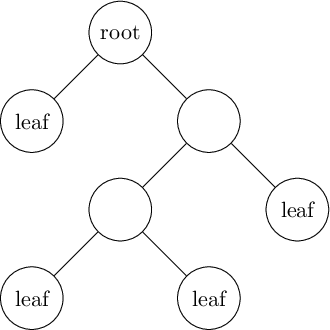
\includegraphics[width=0.4\textwidth]{xcas-tree.png}
\end{center}
which looks like an upside-down tree; the root is at the
top and the leaves are at the bottom. 

Given an expression, the nodes of the corresponding
tree\index{expression tree} are the functions, operators, variables
and constants.  The children of a function node are its arguments, the
children of an operator node are its operands, and the constants and
variables will be the leaves.  For example, the tree for $\sin(2*x +
y)$ will look like
\begin{center}
  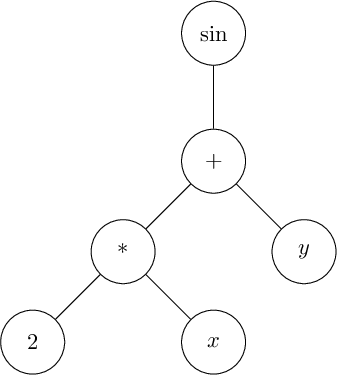
\includegraphics[width=0.4\textwidth]{xcas-expr-tree.png}
\end{center}
A subexpression\index{subexpression} of an expression will be a
selected node together with the nodes below it.  For example, both
$2*x$ and $2*x+y$ are subexpressions of $\sin(2*x+y)$, but $x+y$ is
not.

A subexpression of the contents of the expression editor can be
selected with the mouse; the selection will appear white on a black
background.  A subexpression can also be chosen with the keyboard
using the arrow keys.  Given a selection:
\begin{itemize}
  \item
  The up arrow will go to the parent node.
  \item
  The down arrow will go to the leftmost child node.
  \item
  The right and left arrows will go to the right and left sibling nodes.
  \item
  The control key with the right and left arrows will switch the
  selection with the corresponding sibling.
  \item
  If a constant or variable is selected, the backspace key will delete
  it.  For other selections, backspace will delete the function or
  operator, and another backspace will delete the arguments or operands.
\end{itemize}

You can use the arrow keys to navigate the tree structure of an
expression, which isn't always evident by looking at the expression
itself.  For example, suppose you enter \texttt{x*y*z} in the editor.
The two multiplications will be a different levels; the tree will look
like
\begin{center}
  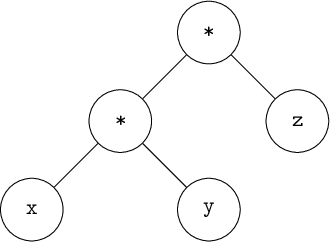
\includegraphics[width=0.4\textwidth]{xcas-xyz-tree.png}
\end{center}
If you select the entire expression with the up arrow and then go to
the \texttt{M} menu to the right of the line and choose eval, then the
expression will look the same but, as you can check by navigating it
with the arrow keys, the tree will look like
\begin{center}
  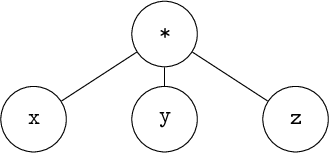
\includegraphics[width=0.4\textwidth]{xcas-xyz-tree2.png}
\end{center}

\subsection{Manipulating subexpressions\index{subexpressions}}

If a subexpression is selected in the expression editor, then any menu
command will be applied to that subexpression.  

For example, suppose that you enter the expression
\begin{center}
  {\tt (x+1)*(x+2)*(x-1)}
\end{center}
in the expression editor.  Note that you can use the abilities of the
editor to make this easier.  First, enter \texttt{x+1}.  Select this
with the up arrow, then type \texttt{*} followed by \texttt{x+2}.  Select
the \texttt{x+2} with the up arrow and then type \texttt{*} followed
by \texttt{x-1}.  Using the up arrow again will select the \texttt{x-1}.
Select the entire expression with the up arrow, and then select
\texttt{eval} from the \texttt{M} menu.  This will put all factors at
the same level.  Suppose you want the factors \texttt{(x+1)*(x+2)} to
be expanded.  You could select \texttt{(x+1)*(x+2)} with the mouse and
do one of the following:
\begin{itemize}
  \item
  Select the
  \texttt{Expression$\blacktriangleright$Misc$\blacktriangleright$normal}
  menu item.  You will then have \texttt{normal((x+1)*(x+2))*(x-1)} in
  the editor.  If you hit enter, the result $(x^2 + 3x + 2)*(x-1)$ will
  appear in the output window.
  \item
  Again, select the   
  \texttt{Expression$\blacktriangleright$Misc$\blacktriangleright$normal}
  menu item, so again you have \texttt{normal((x+1)*(x+2))*(x-1)} in
  the editor.  Now if you select \texttt{eval} from the \texttt{M}
  menu, then the expression in the editor will become the result
  $(x^2 + 3x + 2)*(x-1)$, which you can continue editing.
  \item
  Choose \texttt{normal} from the \texttt{M} menu.  This will apply
  normal to the selection, and again you will have the result
  $(x^2 + 3x + 2)*(x-1)$ in the editor.
\end{itemize}

There are also keystroke commands that you can use to operate
on subexpressions that you've selected.  There are the usual
\texttt{Ctrl+Z} and \texttt{Ctrl+Y} for undoing and redoing.  Some of
the others are given in the following table.

\begin{center}
\begin{tabular}{|p{.20\textwidth}|p{.6\textwidth}|}
\hline
\textbf{Key} & \textbf{Action on selection}\\
%\multicolumn{2}{|c|}{\textbf{Conversions}}\\
\hline\hline
\texttt{Ctrl+D}   & differentiate\\
\texttt{Ctrl+F} & factor\\
\texttt{Ctrl+L} & limit\\
\texttt{Ctrl+N} & normalize\\
\texttt{Ctrl+P} & partial fraction\\
\texttt{Ctrl+R} & integrate\\
\texttt{Ctrl+S} & simplify\\
\texttt{Ctrl+T} & copy \LaTeX{} version to clipboard\\
\hline
\end{tabular}
\end{center}

\section{Previous results}

The \texttt{ans\index{ans}} command will return the results of previous commands.
The input to \texttt{ans} is the number of the command, beginning with
0.  If the first command that you enter is 
\begin{center}
  {\tt 2+5}
\end{center}
resulting in
\begin{center}
  {\tt 7}
\end{center}
then later references to \texttt{ans(0)} will evaluate to \texttt{7}.

Note that the argument to \texttt{ans} doesn't correspond to the line
number in \texttt{Xcas}.  For one thing, the line numbers begin at 1.
What's more, if you go back and re-evaluate a previous line, then that
will become part of the commands that \texttt{ans} keeps track of.

If you give \texttt{ans} a negative number, then it counts backwards
from the current input.  To get the latest output, for
example, you can use \texttt{ans(-1)}.    With no argument,
\texttt{ans()} wil also return the latest output.

Similarly, \texttt{quest\index{quest}} will return the previous inputs.  Since
these will often be simplified to be the same as the output,
\texttt{quest($n$)} sometimes has the same value as \texttt{ans($n$)}.

You can also use \texttt{Ctrl} plus the arrow keys to scroll through
previous inputs.  With the cursor on the command line,
\texttt{Ctrl+uparrow} will go backwards in the list of previous
commands and \texttt{Ctrl+downarrow} will go forwards.

\section{Spreadsheet}
\index{spreadsheet}

\subsection{Opening a spreadsheet}

You can open a spreadsheet (or a matrix editor) with the
\texttt{Spreadsheet$\blacktriangleright$New Spreadsheet} menu item or
with the key \texttt{Alt+T}.

When you open a new spreadsheet, you will be given a configuration screen.  
The configuration screen allows you to set the following options:
\begin{itemize}
  \item
  \texttt{Variable}
  The name of the file where the spreadsheet will be
  saved.
  \item
  \texttt{Rows} and \texttt{Columns}
  The number of rows and columns in the spreadsheet.  
  \item
  \texttt{Eval}
  Whether or not to automatically re-evaluate the entries in the
  spreadsheet after each change.  If this is not checked, then you can
  re-evaluate the spreadsheet with the \texttt{eval} button on the
  spreadsheet menu bar.
  \item
  \texttt{Distribute}
  Whether or not entering a matrix into a cell will keep the entry in
  a single cell or distribute it across an appropriate array of cells.
  \item
  \texttt{Landscape}
  Whether the graphical representation of the spreadsheet should be
  displayed below the spreadsheet or to the right of the spreadsheet.
  If this is checked, it will be displayed below the spreadsheet.
  \item
  \texttt{Move right}
  Whether or not to move to the cell to the right of the current cell
  when data is entered.  If this is not checked, you will be moved to
  the cell below the current cell.
  \item
  \texttt{Spreadsheet}
  Whether to format a spreadsheet or a matrix.
  \item
  \texttt{Graph}
  Whether or not to display the graphical representation of the
  spreadsheet. 
  % \item
  % \texttt{Undo history}
  % \item
  % \texttt{Init sheet}
\end{itemize}
The configuration screen can be reopened with the
\texttt{Edit$\blacktriangleright$Configuration$\blacktriangleright$Cfg
window} menu attached to the spreadsheet.

\subsection{The spreadsheet window}

When you open a spreadsheet, the input line will become the
spreadsheet.
\begin{center}
\includeimage{xcas-spreadsheet.png}
\end{center}
The top will be a menu bar with
\texttt{Table}, \texttt{Edit} and \texttt{Maths} menus as well as
\texttt{eval}, \texttt{val}, \texttt{init}, \texttt{2-d} and
\texttt{3-d} buttons. To the right will be the name of
the file the spreadsheet will be saved into. Below the menu bar will
be two boxes; a box which displays the active cell (and can be used to
choose a cell) and a command line to enter information into the cell.
Below that will be a status line, you can click on this to return to
the configuration screen.

%% \section{Deletions}?

\section{Variables}

\subsection{Variable names}

A variable\index{variable} or function name is a sequence of letters,
numbers and underscores that begins with a letter.  If you define your
own variable or function, you can't use the names of built-in
variables or functions, or other keywords reserved by \texttt{Xcas}.

\subsection{The \texttt{CST} variable}\index{CST}
\label{ssec:cst}

The menu available with the \texttt{cust} button on the onscreen
keyboard is defined with the \texttt{CST} variable.  It is a list
where each list item determines a menu item; a list item is either a
builtin command name or a list itself consisting of a string to be
displayed in the menu and the input to be entered when the item is
selected.  
             
For example, to create a custom defined menu with the builtin function
\texttt{diff}, a user defined function \texttt{foo}, and a menu item
to insert the number $22/7$, you can set
\begin{center}
  \tt
  CST := [diff,["foo",foo],["My pi approx",22/7]]
\end{center}

Note that if the input to be entered is a variable and the variable
has a value when \texttt{CST} is defined, then \texttt{CST} will
contain the value of the variable.  For example,\\
Input:
\begin{center}
  \tt
  app := 22/7\\
  CST := [diff,["foo",foo],["My pi approx",app]]  
\end{center}
will be equivalent to the previous definition of \texttt{CST}.
However, if the variable does not have a value when \texttt{CST} is
defined, for example,
Input:
\begin{center}
  \tt
  CST := [diff,["foo",foo],["My pi approx",app]]\\
  app := 22/7
\end{center}
will behave as the previous values, to begin with, but in this case if
the variable \texttt{app} is changed, so will the the result of
pressing the \texttt{My pi approx} button.

Since \texttt{CST} is a list, a function can be added to the
\texttt{cust} menu with the \texttt{concat} command;\\
Input:
\begin{center}
  \tt
  CST := concat(CST,evalc)
\end{center}
will add the \texttt{evalc} command to the \texttt{cust} menu.

\subsection{Assigning values: \texttt{:= => = assign sto Store}}\index{:=}\index{=>}\index{=}\index{assign}\index{sto}\index{Store}

You can assign a value to a variable with the \texttt{:=}
operator. For example, to give the variable \texttt{a} the value of
\texttt{4}, you can enter
\begin{center}
  {\tt a := 4}
\end{center}
Alternatively, you can use the \texttt{=>} operator; when
you use this operator, the value comes before the variable;
\begin{center}
  {\tt 4 => a}
\end{center}
The function \texttt{sto} or \texttt{Store}
can also be used; again, the value comes before the variable
\begin{center}
  {\tt sto(4,a)}
\end{center}
After any one of these commands, any time you use the variable
\texttt{a} in an expression, it will be replaced by \texttt{4}.

You can use sequences or lists to make multiple assignments at the
same time. For example,
\begin{center}
{\tt (a,b,c) := (1,2,3)}
\end{center}
will assign \texttt{a} the value \texttt{1}, \texttt{b} the value
\texttt{2} and \texttt{c} the value \texttt{3}.   Note that this can
be used to switch the values of two variables; with \texttt{a} and
\texttt{b} as above, the command
\begin{center}
{\tt (a,b) := (b,a)}
\end{center}
will set \texttt{a} equal to \texttt{b}'s original value, namely
\texttt{2}, and will set \texttt{b} equal to \texttt{a}'s original
value, namely \texttt{1}.

Another way to assign values to variables, useful in Maple mode, is
with the \texttt{assign} command. If you enter
\begin{center}
  {\tt assign(a,3)}
\end{center}
or
\begin{center}
  {\tt assign(a = 3)}
\end{center}
then \texttt{a} will have the value \texttt{3}.  You can assign
multiple values at once; if you enter
\begin{center}
  {\tt assign([a = 1, b = 2])}
\end{center}
then \texttt{a} will have the value \texttt{1} and \texttt{b} will
have the value \texttt{2}.  This command can be useful in Maple mode,
where solutions of equations are returned as equations.  For example,
if you enter (in Maple mode)
\begin{center}
  {\tt sol := solve([x + y = 1, y = 2])}
\end{center}
you will get
\begin{center}
  {\tt [x = -1, y = 2]}
\end{center}
If you then enter
\begin{center}
  {\tt assign(sol)}
\end{center}
the variable \texttt{x} will have value \texttt{-1} and \texttt{y}
will have the value \texttt{2}.  This same effect can be achieved in
standard \texttt{Xcas} mode, where
\begin{center}
  {\tt sol := solve([x + y = 1, y = 2])}
\end{center}
will return
\begin{center}
  {\tt [[x = -1, y = 2]]}
\end{center}
In this case, the command
\begin{center}
  {\tt [x,y] := sol[0]}
\end{center}
will assign \texttt{x} the value \texttt{-1} and \texttt{y} the value
\texttt{2}.

\subsection{Assignment by reference: \texttt{=<}}\index{=<}
\label{subsec:refassign}
A list is simply a sequence of values separated by commas and
delimited by \texttt{[} and \texttt{]} (see section \ref{sec:seq}).
Suppose you give the variable \texttt{a} the value \texttt{[1,1,3,4,5]},
\begin{center}
 {\tt  a := [1,2,3,4,5]}
\end{center}
If you later assign to \texttt{a} the value \texttt{[1,2,3,4,5]}, then
a new list is created.  It may be better to just change the second
value in the original list by reference.  This can be done with the
\texttt{=<} command.  Recalling that lists are indexed beginning at 0,
the command
\begin{center}
  {\tt a[1] =< 2}
\end{center}
will simply change the value of the second element of the list instead
of creating a new list, and is a more efficient way to change the
value of \texttt{a} to \texttt{[1,2,3,4,5]}. 

\subsection{Copying values of list: \texttt{copy}}\index{copy}

If you enter
\begin{center}
  {\tt list1 := [1,2,3]}
\end{center}
and then 
\begin{center}
  {\tt list2 := list1}
\end{center}
then \texttt{list1} and \texttt{list2} will be equal to the same list,
not simply two lists with the same elements.  In particular, if you
change (by reference) the value of an element of \texttt{list1}, then
the change will also be reflected in \texttt{list2}.  For example, if
you enter
\begin{center}
  {\tt list1[1] =< 5}
\end{center}
then both \texttt{list1} and \texttt{list2} will be equal to
\texttt{[1,5,3]}.

The \texttt{copy} command will create a copy of a list (or
vector or matrix) which is equal to the original list, but distinct
from it.  For example, if you enter
\begin{center}
  {\tt list1 := [1,2,3]}
\end{center}
and then 
\begin{center}
  {\tt list2 := copy(list1)}
\end{center}
then \texttt{list1} and \texttt{list2} will both be \texttt{[1,2,3]},
but now if you enter
\begin{center}
  {\tt list1[1] =< 5}
\end{center}
then both \texttt{list1} will be equal to \texttt{[1,5,3]} but
\texttt{list2} will still be \texttt{[1,2,3]}.

\subsection{Incrementing variables: \texttt{+= -= *= /=}}\index{+=}\index{-=}\index{*=}\index{/=}

You can increase the value of a variable \texttt{a} by \texttt{4}, for
example, with
\begin{center}
  {\tt a := a + 4}
\end{center}
If beforehand \texttt{a} were equal to \texttt{4}, it would now be
equal to \texttt{8}.  A shorthand way of doing this is with the
\texttt{+=}\index{+=} operator;
\begin{center}
  {\tt a += 4}
\end{center}
will also increase the value of \texttt{a} by \texttt{4}.

Similar shorthands exist for subtraction, multiplication and division.
If \texttt{a} is equal to \texttt{8} and you enter
\begin{center}
  {\tt a -= 2}
\end{center}
then \texttt{a} will be equal to \texttt{6}.  If you follow this with
\begin{center}
  {\tt a *= 3}
\end{center}
then \texttt{a} will be equal to \texttt{18}, and finally
\begin{center}
  {\tt a /= 9}
\end{center}
will end with \texttt{a} equal to \texttt{2}.


\subsection{Storing and recalling variables and their values: \texttt{archive unarchive}}\index{archive}\index{unarchive}

You can store variables and their values for later use in a file of
your choosing with the \texttt{archive} function.  This
function takes two arguments, a filename to store the variables in and
a variable or list of variables.

If you have given the variable \texttt{a} the value \texttt{2} and the
variable \texttt{bee} the value \texttt{"letter"} (a string), then
entering
\begin{center}
  {\tt archive("foo",[a,bee])}
\end{center}
will create a file named ``\texttt{foo}'' which contains the values
\texttt{2} and \texttt{"letter"} in a format meant to be efficiently
read by \texttt{Xcas}.

You can recall the values stored by \texttt{archive} with the
\texttt{unarchive} command, which takes a file name
as argument.  If the file ``\texttt{foo}'' is as above, then 
\begin{center}
  {\tt unarchive("foo")}
\end{center}
will result in
\begin{center}
  {\tt [2, letter]}
\end{center}
If you want to reassign these values to \texttt{a} and \texttt{bee},
you can enter
\begin{center}
  {\tt [a,bee] := unarchive("foo")}
\end{center}

\subsection{Copying variables: \texttt{CopyVar}}\index{CopyVar}
\label{subsec:copyvar}

If a variable has a value, such as
\begin{center}
  {\tt a := 1}
\end{center}
and you set a second variable to the first variable
\begin{center}
  {\tt b := a}
\end{center}
the new variable will have the same value as the first; in this case
\texttt{b} will be equal to \texttt{1}.  If you later give the first
variable a new value;
\begin{center}
  {\tt a := 5}
\end{center}
the new value will still have the old value, in this case, \texttt{b}
will still be equal to \texttt{1}.

The \texttt{CopyVar} command will copy one variable to
another without evaluating the first variable; the new variable will
simply be a copy of the first.  With \texttt{a} having the value of
\texttt{5}, as above, the command
\begin{center}
  {\tt CopyVar(a,c)}
\end{center}
will make \texttt{c} a copy of the variable \texttt{a}, so it will
have the value \texttt{5} also.  If you now change the value of
\texttt{a}
\begin{center}
  {\tt a := 10}
\end{center}
then the value of \texttt{c} will also change; here, \texttt{c} will
now have the value \texttt{10}.

\subsection{Assumptions on variables: \texttt{about additionally assume purge supposons and or}}\index{about}\index{assume}\index{purge}\index{supposons}\index{additionally}\index{and}\index{or}

If you enter
\begin{center}
  {\tt abs(var)}
\end{center}
the \texttt{Xcas} will return it unevaluated, since \texttt{Xcas}
doesn't know what type of value the variable is supposed to represent.

The \texttt{assume} (or
\texttt{supposons}) command will let you tell
\texttt{Xcas} some properties of a variable without giving the
variable a specific value.  For example, if you enter
\begin{center}
  {\tt assume(var > 0)}
\end{center}
then \texttt{Xcas} will assume that \texttt{var} is a positive real
number, and so for example
\begin{center}
  {\tt abs(var)}
\end{center}
will be evaluated to
\begin{center}
   {\tt var}
\end{center}

You can put one or more conditions in the \texttt{assume} command by
combining them with \texttt{and} and \texttt{or}.
For example, if you want the variable \texttt{a} to be in $[2,4) \cup
(6,\infty)$, you can enter
\begin{center}
  {\tt assume((a >= 2 and a < 4) or a > 6)}
\end{center}

If a variable has attached assumptions, then making another assumption
with \texttt{assume} will remove the original assumptions.  To add
extra assumptions, you can either use the
\texttt{additionally} command or give
\texttt{assume} a second argument of
\texttt{additionally\index{additionally@\textit{additionally}}}.  If
you assume that $b > 0$ with
\begin{center}
  {\tt assume(b > 0)}
\end{center}
and you want to add the condition that $b < 1$, you can either enter
\begin{center}
  {\tt assume(b < 1, additionally)}
\end{center}
or
\begin{center}
  {\tt additionally(b < 1)}
\end{center}

As well as equalities and inequalities, you can make assumptions about
the domain of a variable.  If you want \texttt{n} to represent a
positive integer\index{integer@\textit{integer}}, for example, you can enter
\begin{center}
  {\tt assume(n, integer)}
\end{center}
If you want \texttt{n} to be a positive integer, you can add the
condition
\begin{center}
  {\tt additionally(n > 0)}
\end{center}

You can use the \texttt{about} command to check the assumptions on a
variable; for the above positive integer \texttt{n}, if you enter
\begin{center}
  {\tt about(n)}
\end{center}
you will get
\begin{center}
  {\tt assume[integer,[line[0,+infinity]],[0]]}
\end{center}
The first element tells you that \texttt{n} is an integer, the second
element tells you that \texttt{n} is between \texttt{0} and
\texttt{+infinity}, and the third element tells you that the value
\texttt{0} is excluded.

If you assume that a variable is equal to a specific value, such as
\begin{center}
  {\tt assume(c = 2)}
\end{center}
then by default the variable \texttt{c} will remain unevaluated in
later levels.  If you want an expression involving \texttt{c} to be
evaluated, you would need to put the expression inside the
\texttt{evalf\index{evalf}} command; if you enter
\begin{center}
  {\tt evalf(c\^{}2 + 3)}
\end{center}
then you will get 
\begin{center}
  {\tt 7.0}
\end{center}
Right below the \texttt{assume(c = 2)} command line
there will be a slider, namely arrows pointing left and right with the
value \texttt{2} between them.  These
can be used to change the values of \texttt{c}.  If you click on the
right arrow, the \texttt{assume(c = 2)} command will transform to
\begin{center}
  {\tt assume(c=[2.2,-10.0,10.0,0.0])}
\end{center}
and the value between the arrows will be \texttt{2.2}.  Also, any
later levels where the variable \texttt{c} is evaluated will be
re-evaluated with the value of \texttt{c} now \texttt{2.2}.  The
output to \texttt{evalf(c\^{}2 + 3} will become
\begin{center}
  {\tt 7.84}
\end{center}
The \texttt{-10.0} and \texttt{10.0} in the \texttt{assume} line
represent the smallest and largest values that \texttt{c} can become
using the sliders.  You can set them yourself in the \texttt{assume}
command, as well as the increment that the value will change; if you
want \texttt{c} to start with the value \texttt{5} and vary between
\texttt{2} and \texttt{8} in increments of \texttt{0.05}, then you can
enter
\begin{center}
  {\tt assume(c = [5,2,8,0.05])}
\end{center}

You can remove any assumptions you have made about a variable with the
\texttt{purge} command; if you enter
\begin{center}
  {\tt purge(a)}
\end{center}
then \texttt{a} will no longer have any assumptions made about it.
You can remove assumptions from more than one variable at a time;
\begin{center}
  {\tt purge(a,b)}
\end{center}
will remove any assumptions about \texttt{a} and \texttt{b}.

\subsection{Unassigning variables: \texttt{VARS purge DelVar del restart rm\_a\_z rm\_all\_vars}}\index{VARS}\index{purge}\index{restart}\index{rm\_a\_z}\index{rm\_all\_vars}\index{DelVar}\index{del}

The \texttt{VARS()} command will list the variables to which you have
assigned values or assumptions.  If you begin by entering
\begin{center}
  {\tt a := 1}
\end{center}
and
\begin{center}
  {\tt anothervar := 2}
\end{center}
then 
\begin{center}
  {\tt VARS()}
\end{center}
will return
\begin{center}
  {\tt [a, anothervar]}
\end{center}

The \texttt{purge} command will clear the values and
assumptions you make on variables.  To clear the values and
assumptions on \texttt{a}, for example, you can enter\\
Input:
\begin{center}
  \tt
  purge(a)
\end{center}
For \texttt{TI} compatibility, you can also enter\\
Input:
\begin{center}
  \tt
  DelVar a
\end{center}
and for Python compatibility, you can also enter
Output:
\begin{center}
  \tt
 del a 
\end{center}

To clear the values and assumptions you have made on all variables you
can use the
\begin{center}
  {\tt restart}
\end{center}
or
\begin{center}
  {\tt rm\_all\_vars()}
\end{center}
command.  The command \texttt{rm\_a\_z} will clear the values and
assumptions of the variables with single lowercase letter names.  If
you have variables names \texttt{A,B,a,b,myvar}, then after\\
Input:
\begin{center}
  \tt
 rm\_a\_z() 
\end{center}
you will only have the variables named \texttt{A,B,myvar}.

\section{Functions}

\subsection{Defining functions}

You can use the \texttt{:=}\index{:=} and \texttt{=>}\index{=>}
operators to define functions; both
\begin{center}
  {\tt f(x) := x\^{}2}
\end{center}
and
\begin{center}
  {\tt x\^{}2 => f(x)}
\end{center}
give the name \texttt{f} to the function which takes a value and 
returns the square of the value.  If you then enter
\begin{center}
  {\tt f(3)}
\end{center}
you will get
\begin{center}
  {\tt 9}
\end{center}

You can give \texttt{Xcas} a function without a name with the
\texttt{->}\index{->} operator; the squaring function can be written
without a name as
\begin{center}
  {\tt x -> x\^{}2}
\end{center}
You can use this form of the function to assign it to a name; both
\begin{center}
  {\tt f := x -> x\^{}2}
\end{center}
and
\begin{center}
  {\tt x -> x\^{}2 => f}
\end{center}
are alternate ways to define \texttt{f} as the squaring function.

You can similarly define functions of more than one variable.  For
example, to define a function which takes the lengths of the two legs
of a right triangle and returns the hypotenuse, you could enter
\begin{center}
  {\tt hypot(a,b) := sqrt(a\^{}2 + b\^{}2)}
\end{center}
or
\begin{center}
  {\tt hypot := (a,b) -> sqrt(a\^{}2 + b\^{}2)}
\end{center}

\subsection{Defining piecewise defined functions}
\index{piecewise defined functions}
\label{subsec:piecewise}

You can use \texttt{Xcas}'s control structures to define functions not
given by a single simple formula.  Notably, you can use the
\texttt{ifte\index{ifte}} command or \texttt{? :\index{? :}} operator
to define piecewise-defined functions.

The \texttt{ifte} command takes three arguments; the first argument is
a condition, the second argument tells the command what to return when
the condition is true, and the third argument tells the command what
to return when the condition is false.  For example, you could define
your own absolute value function with
\begin{center}
  {\tt myabs(x) := ifte(x >= 0, x -1*x)}
\end{center}
Afterwards, for example, entering
\begin{center}
  {\tt myabs(-4)}
\end{center}
will return
\begin{center}
  {\tt 4}
\end{center}
However, this will return an error if it can't evaluate the
conditional.  For example, if you enter
\begin{center}
  {\tt myabs(x)}
\end{center}
you will get the error
\begin{center}
  {\tt Ifte: Unable to check test Error: Bad Argument Value}
\end{center}

The \texttt{? :}\index{? :} construct behaves similarly to \texttt{ifte} but is
structured differently.  Here, the condition comes first, followed by
\texttt{?}, then what to return if the condition is true, followed by
the \texttt{:}, and then what to return if the condition is false.
You could define your absolute value function with
\begin{center}
  {\tt myabs(x) := (x >= 0)? x: -1*x}
\end{center}
If you enter
\begin{center}
  {\tt myabs(-4)}
\end{center}
you will again get
\begin{center}
  {\tt 4}
\end{center}
but now if the conditional can't be evaluated, you won't get an error.
\begin{center}
  {\tt myabs(x)}
\end{center}
will return
\begin{center}
  {\tt ((x >= 0)? x: -x)}
\end{center}

The \texttt{when\index{when}} and \texttt{IFTE\index{IFTE}} commands
are synonyms for the \texttt{? :} construct; 
\begin{center}
  {\tt (\textit{condition})? \textit{true-result}: \textit{false-result}}
\end{center}
\begin{center}
  {\tt when(\textit{condition}, \textit{true-result}, \textit{false-result})}
\end{center}
and
\begin{center}
  {\tt IFTE(\textit{condition}, \textit{true-result}, \textit{false-result})}
\end{center}
all represent the same expression.

If you want to define a function with several pieces, it may be
simpler to use the \texttt{piecewise\index{piecewise}} function.  The
arguments to this function are alternately conditions and results to
return if the condition is true, with the last argument being what to
return if none of the conditions are true.  For example, to define the
function given by
\[
f(x) = 
\begin{cases}
-2 & \text{if } x < -2\\
3x+4 & \text{if } -2 \le x < -1\\
1 & \text{if } -1 \le x < 0\\
x + 1 & \text{if } x \ge 0
\end{cases}
\]
you can enter
\begin{center}
  {\tt f(x) := piecewise(x < -2, -2, x < -1, 3*x+4, x < 0, 1, x + 1)}
\end{center}

\section{Directories}
\index{directories}

\subsection{Working directories}

\texttt{Xcas} has a working directory that it uses to store files that
it creates; typically the user's home directory.  You can print the
name of the current working directory with the
\texttt{pwd()}\index{pwd} command; if you enter
\begin{center}
  {\tt pwd()}
\end{center}
you might get something like
\begin{center}
  {\tt /home/username}
\end{center}

You can change the working directory with the \texttt{cd\index{cd}}
command; if you enter
\begin{center}
  {\tt cd("foo")}
\end{center}
or (on a Unix system)
\begin{center}
  {\tt cd("/home/username/foo")}
\end{center}
will change to the directory \texttt{foo}, if it exists.
Afterwards, any files that you save from \texttt{Xcas} will be in that
directory.  

If you have values saved in a file, then you'll need to be in that
working directory to load it.  Note that if you have the same file
name in different directories, then the result of loading the file
name will depend on which directory you are in.

\subsection{Reading files: \texttt{read load}}\index{read}\index{load}

If you have a function or other \texttt{Xcas} information in a file,
you can load it with the \texttt{read} function.  If the
file is named \texttt{myfunction.cxx}, then
\begin{center}
  {\tt read("myfunction.cxx")}
\end{center}
will load the file, as long as the directory is in the current working
directory.  If the file is in a different directory, you can still
load it by giving the path to the file,
\begin{center}
  {\tt read("/path/to/file/myfunction.cxx")}
\end{center}

While \texttt{read} can be used to load files containing \texttt{Xcas}
functions, which typically end in \texttt{.cxx}, if you want to load a
saved session you should use the \texttt{load} function;
\begin{center}
  {\tt load("mysession.cas")}
\end{center}

\subsection{Internal directories: \texttt{NewFold SetFold GetFold DelFold VARS}}\index{NewFold}\index{SetFold}\index{GetFold}\index{DelFold}\index{VARS}\index{internal directories}

You can create a directory that isn't actually on your hard drive but
is treated like one from \texttt{Xcas}.  You can create such an
internal directory with the \texttt{NewFold} command,
which takes a variable name as an argument. If you enter
\begin{center}
  {\tt NewFold(MyIntDir)}
\end{center}
then there will be a new internal directory named \texttt{MyIntDir}.
Internal directories will also be listed with the
\texttt{VARS()}
command. To actually use this directory, you'll have to use the
\texttt{SetFold} command;
\begin{center}
  {\tt SetFold(MyIntDir)}
\end{center}
Finally, we can print out the internal directory that we are in with
the \texttt{GetFold} command; entering
\begin{center}
  {\tt GetFold()}
\end{center}
will result in
\begin{center}
  {\tt MyIntDir}
\end{center}
Afterwards, if this directory is empty, you can delete it with the
\texttt{DelFold} command;
\begin{center}
  {\tt DelFold(MyIntDir)}
\end{center}

\chapter{The CAS functions}\label{sec:cas}

\section{Symbolic constants : {\tt e pi infinity inf i euler\_gamma}}
\index{e}\index{\%e}\index{pi}\index{\%pi}\index{i}\index{\%i}
\index{+infinity}\index{-infinity}\index{infinity}
\index{euler\_gamma}\index{inf}\index{-inf}

\noindent {\tt e} (or \texttt{\%e}) is the number $\exp(1)$;\\ 
{\tt pi} (or \texttt{\%pi}) is the number $\pi$.\\
{\tt infinity} is unsigned $\infty$.\\
{\tt +infinity} or {\tt inf} is $+\infty$.\\
{\tt -infinity} or {\tt -inf} is $-\infty$.\\
{\tt i} (or \texttt{\%i}) is the complex number $i$.\\
{\tt euler\_gamma} is Euler's constant $\gamma$; namely,
\texttt{limit(sum(1/k,k,1,n)-ln(n),n,+infinity)}

\section{Booleans}
\label{sec:boolean}
\subsection{The values of a boolean : {\tt true false}}\index{true}\index{false}\index{TRUE}\index{FALSE}
The value of a boolean is {\tt true} or {\tt false}.\\
The synonyms are :\\
{\tt true} or {\tt TRUE} or {\tt 1},\\
{\tt false} or {\tt FALSE} or {\tt 0}.\\
Tests or conditions are boolean functions.

\subsection{Tests : {\tt == != > >= < =<}}\index{==}\index{>}\index{<}\index{>=}\index{<=}\index{\symbol{33}=}
{\tt ==, !=, >, >=, <, =<} are infixed operators.\\
{\tt a==b} tests the equality between {\tt a} and {\tt b} and returns {\tt 1} 
if {\tt a} is equal to {\tt b} and {\tt 0} otherwise.\\ 
{\tt a!=b} returns {\tt 1} if {\tt a} and {\tt b} are different and {\tt 0} 
otherwise.\\
 {\tt a>=b} returns {\tt 1} if {\tt a} is greater than or equal to {\tt b} 
and {\tt 0} otherwise.\\ 
{\tt a>b} returns {\tt 1} if {\tt a} is strictly greater than {\tt b}
and {\tt 0} otherwise.\\ 
{\tt a<=b} returns {\tt 1} if {\tt a} is less than or equal to {\tt b} and 
{\tt 0} otherwise.\\
{\tt a<b} returns {\tt 1} if {\tt a} is strictly less than {\tt b} 
and {\tt 0} otherwise.\\ 
To write an algebraic function having the same result as an 
{\tt if...then...else}, we use the boolean function {\tt ifte}.\\
For example :  
\begin{center}{\tt f(x):=ifte(x>0,true,false)}\end{center}
defines the boolean function $f$ such that {\tt f(x)= true} if 
$x \in (0;+\infty[$ and {\tt f(x)=false} if $x \in (-\infty;0]$.\\
Input :
\begin{center}{\tt f(0)==0}\end{center}
Output :
\begin{center}{\tt 1}\end{center}
{\bf Look out !}\\
{\tt a=b}  is not a boolean !!!!\\
{\tt a==b} is a boolean.\\

\subsection{Boolean operators  : {\tt or xor and not}}\index{or|textbf}\index{not|textbf}\index{and|textbf}\index{$\bigparallel$}\index{\&\&|textbf}\index{\symbol{33}=|textbf}\index{xor|textbf}
{\tt or} (or {\tt ||}), {\tt xor}, {\tt and} (or {\tt \&\&})  are infixed 
operators.\\
{\tt not} is a prefixed operators.\\ 
If {\tt a} and {\tt b} are two booleans :\\
{\tt (a or b)}  {\tt (a || b)} returns  {\tt 0} (or {\tt false}) if {\tt a} and
{\tt b} are equal to 0  and returns {\tt 1} (or {\tt true}) otherwise.\\ 
{\tt (a xor b)}   returns {\tt 1} if {\tt a} is equal to 1 and {\tt b} is
equal to 0 or if {\tt a} is equal to 0 and {\tt b} is equal to 1  and  returns 0
 if {\tt a} and {\tt b} are equal to 0
 or if  {\tt a} and {\tt b}  are equal to 1 (it is the "exclusive or").\\ 
{\tt (a and b)} or {\tt (a \&\& b)}  returns {\tt 1} (or {\tt true}) if {\tt a}
 and {\tt b}  are equal to 1 and {\tt 0} (or {\tt false})  otherwise.\\
{\tt not(a)} returns {\tt 1} (or {\tt true}) if {\tt a}  is equal to 0 (or 
{\tt false}), and {\tt 0} (or {\tt false})  if {\tt a}  is equal to 1 (or 
{\tt true}).\\ 
Input :
\begin{center}{\tt 1>=0 or 1<0}\end{center}
Output :
\begin{center}{\tt 1}\end{center}
Input :
\begin{center}{\tt 1>=0 xor 1>0}\end{center}
Output :
\begin{center}{\tt 0}\end{center}
Input :
\begin{center}{\tt 1>=0 and 1>0}\end{center}
Output :
\begin{center}{\tt 1}\end{center}
Input :
\begin{center}{\tt not(0==0)}\end{center}
Output :
\begin{center}{\tt 0}\end{center}

\subsection{Transform a boolean expression to a list : {\tt exp2list}}\index{exp2list}
\noindent{\tt exp2list} returns the list {\tt [expr0,expr1]} when the argument 
is {\tt (var=expr0) or (var=expr1)}.\\
{\tt exp2list} is used in TI mode for easier processing of the answer to a
{\tt solve} command.\\
Input :
\begin{center}{\tt exp2list((x=2) or (x=0))}\end{center}
Output :
\begin{center}{\tt [2,0]}\end{center}
Input :
\begin{center}{\tt exp2list((x>0) or (x<2))}\end{center}
Output :
\begin{center}{\tt [0,2]}\end{center}
In TI mode input :
\begin{center}{\tt exp2list(solve((x-1)*(x-2)))}\end{center}
Output :
\begin{center}{\tt [1,2]}\end{center}

\subsection{Transform a list into a boolean expression: {\tt list2exp}}\index{list2exp}
\noindent
The \texttt{list2exp} command is the inverse of \texttt{exp2list}.  It
takes two arguments; a list \texttt{[val1, val2, ...]} of values and a variable name
\texttt{var}.\\
\texttt{list2exp} returns the boolean expression \texttt{((var = val1)
or (var = val2) or ...)}.\\
Input:
\begin{center}
  \tt
  list2exp([0,1],a)
\end{center}
Output:
\begin{center}
  \tt
 ((a=0) or (a=1)) 
\end{center}
Input:
\begin{center}
  \tt
  list2exp(solve(x\^{}2-1=0,x),x)
\end{center}
Output:
\begin{center}
  \tt
  ((x=-1) or (x=1))
\end{center}

Alternatively, each element of the list could be a list with $n$ values, followed by a
list of $n$ variables.  The output would be boolean expressions of the
form \texttt{((var1 = val1) and (var2 = val2) ...)} for each
list of $n$ values, combined with \texttt{or}s.
Input:
\begin{center}
  \tt
  list2exp ([[3,9], [-1,1]], [x, y])
\end{center}
Output:
\begin{center}
  \tt
 ((((x=3) and (y=9))) or (((x=-1) and (y=1)))) 
\end{center}

\subsection{Evaluate booleans : {\tt evalb}}\index{evalb}
\noindent Inside Maple, {\tt evalb} evaluates an boolean expression.
Since {\tt Xcas} evaluates booleans automatically, {\tt evalb} is only
here for compatibility and is equivalent to {\tt eval}\\
Input :
\begin{center}{\tt evalb(sqrt(2)>1.41)}\end{center}
or :
\begin{center}{\tt sqrt(2)>1.41}\end{center}
Output :
\begin{center}{\tt 1}\end{center}
Input :
\begin{center}{\tt evalb(sqrt(2)>1.42)}\end{center}
or :
\begin{center}{\tt sqrt(2)>1.42}\end{center}
Output :
\begin{center}{\tt 0}\end{center}

\section{Bitwise operators}
\subsection{Operators {\tt bitor bitxor bitand}}\index{bitor|textbf}\index{bitxor|textbf}\index{bitand|textbf}
The integers may be written using hexadecimal notation 0x...
for example 0x1f represents 16+15=31 in decimal. 
Integers may also be output in hexadecimal notation 
(click on the red CAS status button and select {\tt Base (Integers)}).\\
{\tt bitor} is the logical inclusive {\tt or} (bitwise).\\
Input :
\begin{center}{\tt bitor(0x12,0x38)}\end{center}
or :
\begin{center}{\tt bitor(18,56)}\end{center}
Output :
\begin{center}{\tt 58}\end{center}
because :\\
{\tt 18} is written {\tt 0x12} in base 16 or {\tt 0b010010} in base 2,\\
{\tt 56} is written {\tt 0x38} in base 16 or {\tt 0b111000} in base 2,\\
hence {\tt bitor(18,56)} is {\tt 0b111010} in base 2 and so is equal to 
{\tt 58}.\\

{\tt bitxor} is the logical exclusive {\tt or} (bitwise).\\
Input :
\begin{center}{\tt bitxor(0x12,0x38)}\end{center}
or :
\begin{center}{\tt bitxor(18,56)}\end{center}
Output :
\begin{center}{\tt 42}\end{center}
because :\\
{\tt 18} is written {\tt 0x12} in base 16 and {\tt 0b010010} in base 2,\\
{\tt 56} is written {\tt 0x38} in base 16 and {\tt 0b111000} in base 2,\\
{\tt bitxor(18,56)} is written {\tt 0b101010} in base 2 and so, is equal to 
{\tt 42}.\\

{\tt bitand} is the logical {\tt and} (bitwise).\\
Input :
\begin{center}{\tt bitand(0x12,0x38)}\end{center}
or : 
\begin{center}{\tt bitand(18,56)}\end{center}
Output :
\begin{center}{\tt 16}\end{center}
because :\\
{\tt 18} is written {\tt 0x12} in base 16 and {\tt 0b010010} in base 2,\\
{\tt 56} is written {\tt 0x38} in base 16 and {\tt 0b111000} in base 2,\\
{\tt bitand(18,56)} is written {\tt 0b010000} in base 2 and so is equal to
{\tt 16}.

\subsection{Bitwise Hamming distance : {\tt hamdist}}\index{hamdist|textbf}
The Hamming distance is the number of differences
of the bits of the two arguments.\\
Input :
\begin{center}{\tt hamdist(0x12,0x38)}\end{center}
or : 
\begin{center}{\tt hamdist(18,56)}\end{center}
Output :
\begin{center}{\tt 3}\end{center}
because :\\
{\tt 18}  is written {\tt 0x12} in base 16 and {\tt 0b010010} in base 2,\\
{\tt 56}  is written {\tt 0x38} in base 16 and {\tt 0b111000} in base 2,\\
{\tt hamdist(18,56)} is equal to {\tt 1+0+1+0+1+0} and so is equal to {\tt 3}.

\section{Strings}
\subsection{Character and string : {\tt "}}\index{\symbol{34}|textbf}
\noindent {\tt "} is used to delimit a string.
A character is a string of length one.\\
Do not confuse {\tt "} with
{\tt '} (or {\tt quote}) which is used to avoid evaluation
of an expression \index{quote}. For example,
{\tt "a"} returns a string of one character 
but {\tt 'a'} or {\tt quote(a)} returns
the variable {\tt a} unevaluated.\\

When a string is input in a command line, it is evaluated to itself
hence the output is the same string. Use {\tt +}
to concatenate two strings or a string and another object.\\
Example :\\
Input :
\begin{center}{\tt "Hello"}\end{center}
{\tt "Hello"} is the input and also the output.\\
Input :
\begin{center}{\tt "Hello"+", how are you?"}\end{center}
Output :
\begin{center}{\tt "Hello, how are you?"}\end{center}
Index notation is used to get the n-th character of a string, 
(as for lists). Indices begin at 0 in Xcas mode, 1 in other modes.\\
Example :\\
Input :
\begin{center}{\tt "Hello"[1]}\end{center}
Output :
\begin{center}{\tt "e"}\end{center}

\subsection{The newline character: \texttt{\symbol{92}n}}\index{\symbol{92}n}

A newline can be inserted into a string with \texttt{\symbol{92}n}.\\
Input:
\begin{center}
  \tt
  Hello\symbol{92}nHow are you?
\end{center}
Output:
\begin{center}
  \tt
 Hello\\
 How are you?
\end{center}

\subsection{The length of a string: \texttt{size length}}\index{size}\index{length}
The \texttt{size} (or \texttt{length}) command can take a string as an
argument.  It will return the length of the string.\\
Input:
\begin{center}
  \tt
  size("hello")
\end{center}
Output:
\begin{center}
  \tt
 5 
\end{center}

\subsection{The left and right parts of a string: \texttt{left right}}\index{left}\index{right}

The \texttt{left} command takes two arguments, a string \texttt{s}  and a
non-negative integer \texttt{n}.\\
\texttt{left} returns the first \texttt{n} characters of the string.\\
Input:
\begin{center}
  \tt
  left("hello",3)
\end{center}
Output:
\begin{center}
  \tt
 "hel" 
\end{center}

Similarly, the \texttt{right} command returns the last \texttt{n}
characters.\\\\
Input:
\begin{center}
  \tt
  right("hello",4)
\end{center}
Output:
\begin{center}
  \tt
 "ello" 
\end{center}

\subsection{First character, middle and end of a string : {\tt head mid tail}}\index{head|textbf} \index{tail|textbf}\index{mid}
\begin{itemize}
\item  {\tt head(s)} returns the first character of the string {\tt s}.\\ 
 Input :
\begin{center}{\tt head("Hello")}\end{center}
Output :
\begin{center}{\tt "H"}\end{center}
\item {\tt mid(s,p,q)} returns the part of the string
{\tt s} of size {\tt q} beginning with the character at index {\tt p}.\\
Remember that the first index is 0 in Xcas mode.\\
Input :
\begin{center}{\tt mid("Hello",1,3)}\end{center}
Output :
\begin{center}{\tt "ell"}\end{center}
\item {\tt tail(s)} returns the string  {\tt s} without its first character.\\ 
Input :
\begin{center}{\tt tail("Hello")}\end{center}
Output :
\begin{center}{\tt "ello"}\end{center}
\end{itemize}

\subsection{Concatenation of a sequence of words : {\tt cumSum}}\index{cumSum}
\noindent{\tt cumSum} works on strings like it does on expressions by
doing partial concatenation.\\
{\tt cumSum} takes as argument a list of strings.\\
{\tt cumSum} returns a list of strings where the element of index $k$ is the
concatenation of the strings with indices 0 to $k$ .\\
Input :
\begin{center}{\tt cumSum("Hello, ","is ","that ","you?")}\end{center}
Output :
\begin{center}{\tt "Hello, ","Hello, is ","Hello, is that ","Hello, is that you?}\end{center}

\subsection{ASCII code of a character : {\tt ord}}\index{ord|textbf}
\noindent {\tt ord} takes as argument a string {\tt s} (resp. 
a list {\tt l} of 
strings).\\
{\tt ord} returns the ASCII code of the first character of {\tt s} (resp. the 
list of the ASCII codes of the first character of the elements of {\tt l}).\\
Input :
\begin{center}{\tt ord("a")}\end{center}
Output :
\begin{center}{\tt 97}\end{center}
Input :
\begin{center}{\tt ord("abcd")}\end{center}
Output :
\begin{center}{\tt 97}\end{center} 
Input :
\begin{center}{\tt ord(["abcd","cde"])}\end{center}
Output :
\begin{center}{\tt [97,99]}\end{center} 
Input :
\begin{center}{\tt ord(["a","b","c","d"])}\end{center}
Output :
\begin{center}{\tt [97,98,99,100]}\end{center} 

\subsection{ASCII code of a string : {\tt asc}}\index{asc}
\noindent {\tt asc} takes as argument a string {\tt s}.\\
{\tt asc} returns the list of the ASCII codes of the characters of {\tt s}.\\
Input :
\begin{center}{\tt asc("abcd")}\end{center}
Output :
\begin{center}{\tt [97,98,99,100]}\end{center} 
Input :
\begin{center}{\tt asc("a")}\end{center}
Output :
\begin{center}{\tt [97]}\end{center}

\subsection{String defined by the ASCII codes of its characters : {\tt char}}\index{char}
\noindent {\tt char} takes as argument a list {\tt l} of ASCII codes.\\ 
{\tt char} returns the string whose characters have as ASCII codes the 
elements of the list {\tt l}.\\
Input :
\begin{center}{\tt char([97,98,99,100])}\end{center}
Output :
\begin{center}{\tt "abcd"}\end{center} 
Input :
\begin{center}{\tt char(97)}\end{center}
Output :
\begin{center}{\tt "a"}\end{center}
Input :
\begin{center}{\tt char(353)}\end{center}
Output :
\begin{center}{\tt "a"}\end{center}
because:\\
$353-256=97$.

\subsection{Find a character in a string : {\tt inString}}\index{inString}
\noindent {\tt inString} takes two arguments : a string {\tt S} and a 
character {\tt c}.\\
{\tt inString} tests if the character {\tt c} is in the string {\tt S}.\\
 {\tt inString} returns the index of its first occurrence
or {\tt -1} if {\tt c} is not in {\tt S}.\\
Input :
\begin{center}{\tt inString("abcded","d")}\end{center}
Output :
\begin{center}{\tt  3}\end{center}
Input :
\begin{center}{\tt inString("abcd","e")}\end{center}
Output :
\begin{center}{\tt  -1}\end{center}

\subsection{Concat objects into a string : {\tt cat}}\index{cat|textbf}
\noindent {\tt cat} takes as argument a sequence of objects.\\ 
{\tt cat} concatenates these objects into a string.\\
Input :
\begin{center}{\tt cat("abcd",3,"d")}\end{center}
Output :
\begin{center}{\tt  "abcd3d"}\end{center}
Input :
\begin{center}{\tt c:=5}\end{center}
\begin{center}{\tt cat("abcd",c,"e")}\end{center}
Output :
\begin{center}{\tt  "abcd5e"}\end{center}
Input :
\begin{center}{\tt purge(c)}\end{center}
\begin{center}{\tt cat(15,c,3)}\end{center}
Output :
\begin{center}{\tt  "15c3"}\end{center}

\subsection{Add an object to a string : {\tt +}}\index{+}
\noindent {\tt +} is an infixed operator (resp. {\tt '+'} is a prefixed 
operator).\\
If  {\tt +} (resp.  {\tt '+'}) takes as argument a string (resp.
a sequence of objects with a string as first or second argument), 
the result is the concatenation of these objects into a string.\\
{\bf warning}\\
{\tt +} is infixed and {\tt '+'} is prefixed.\\ 
Input :
\begin{center}{\tt '+'("abcd",3,"d")}\end{center}
Output :
\begin{center}{\tt "abcd"+3+"d"}\end{center}
Output :
\begin{center}{\tt  "abcd3d"}\end{center}
Input :
\begin{center}{\tt c:=5}\end{center}
Then input:
\begin{center}{\tt "abcd"+c+"e"}\end{center}
or :
\begin{center}{\tt '+'("abcd",c,"d")}\end{center}
Output :
\begin{center}{\tt  "abcd5e"}\end{center}

\subsection{Transform an integer into a string : {\tt cat +}}\index{+}\index{cat}
\noindent Use {\tt cat} with the integer as argument, or add the integer
to an empty string\\
Input :
\begin{center}{\tt ""+123}\end{center}
or :
\begin{center}{\tt cat(123)}\end{center}
Output :
\begin{center}{\tt  "123"}\end{center}

\subsection{Transform a string into a number : {\tt expr}}\index{expr|textbf}\label{sec:expr1}
Use {\tt expr}, the parser with a string representing a number.
\begin{itemize}
\item For integers, enter the string representing the integer without
leading 0 for basis 10, with prefix {\tt 0x} for basis 16,
{\tt 0} for basis 8 or {\tt 0b} for basis 2.
Input :
\begin{center}{\tt expr("123")}\end{center}
Output :
\begin{center}{\tt  123}\end{center}
Input :
\begin{center}{\tt expr("0123")}\end{center}
Output :
\begin{center}{\tt  83}\end{center}
because :\\
$1*8^2+2*8+3=83$\\
Input :
\begin{center}{\tt expr("0x12f")}\end{center}
Output :
\begin{center}{\tt 303}\end{center}
Because : $1*16^2+2*16+15=303$
\item For decimal numbers, use a string with a {\tt .} or {\tt e} inside.\\
Input :
\begin{center}{\tt expr("123.4567")}\end{center}
Output :
\begin{center}{\tt  123.4567}\end{center}
Input :
\begin{center}{\tt expr("123e-5")}\end{center}
Output :
\begin{center}{\tt 0.00123}\end{center}
\item Note that {\tt expr} more generally transforms a string 
into a command if the command exists.\\
Input :
\begin{center}{\tt expr("a:=1")}\end{center}
Output :
\begin{center}{\tt 1}\end{center}
Then, input :
\begin{center}{\tt a}\end{center}
Output :
\begin{center}{\tt 1}\end{center}
\end{itemize}

\section{Write an integer in base $b$: {\tt convert}}\index{convert}\index{base@{\sl base}|textbf}
\label{sec:convertbase}

\noindent{\tt convert} or {\tt convertir} can do different kind
of conversions depending on the option given as the second argument.

To convert an integer {\tt n} into the list of its coefficients in
base {\tt b}, the option is {\tt base}. The arguments of {\tt convert} or 
{\tt convertir} are an integer {\tt n}, {\tt base} and {\tt b}, the value of the
 basis.\\
{\tt convert} or {\tt convertir} returns the list of coefficients in a {\tt b} 
basis of the integer {\tt n}.\\
Input :
\begin{center}{\tt convert(123,base,8)}\end{center}
Output :
\begin{center}{\tt [3,7,1]}\end{center}
To check the answer, 
input {\tt expr("0173")} or  {\tt horner(revlist([3,7,1]),8)}
or {\tt convert([3,7,1],base,8)}, the output is {\tt 123}\\
Input :
\begin{center}{\tt convert(142,base,12)}\end{center}
Output :
\begin{center}{\tt [10,11]}\end{center}

To convert the list of coefficients of an integer {\tt n} in base {\tt b},
the option is also {\tt base}. 
{\tt convert} or {\tt convertir} returns the integer {\tt n}.\\ 
Input :
\begin{center}{\tt convert([3,7,1],base,8)}\end{center}
or :
\begin{center}{\tt horner(revlist([3,7,1]),8)}\end{center}
Output :
\begin{center}{\tt 123}\end{center}
Input :
\begin{center}{\tt convert([10,11],base,12)}\end{center}
or :
\begin{center}{\tt horner(revlist([10,11]),12)}\end{center}
Output :
\begin{center}{\tt 142}\end{center}

\section{Integers (and Gaussian Integers)}
 For all functions in this section, you can use Gaussian integers (numbers of 
the form  $a+ib$, where $a$ and $b$ are in  $\mathbb Z$) in place of integers.

\subsection{The factorial : {\tt factorial}}\index{factorial}
{\tt Xcas} can manage integers with unlimited precision, such as the 
following:\\ 
Input :
\begin{center}{\tt factorial(100)}\end{center}
Output :
\begin{verbatim}
   9332621544394415268169923885626670049071596826438162
   1468592963895217599993229915608941463976156518286253
   697920827223758251185210916864000000000000000000000000
\end{verbatim}
\subsection{GCD : {\tt gcd igcd}}\index{gcd|textbf}\index{igcd|textbf}\label{sec:igcd}
\noindent{\tt gcd} or {\tt igcd} denotes the gcd (greatest common divisor)
of several integers (for polynomials, see also \ref{sec:gcd}).\\ 
{\tt gcd} or {\tt igcd} returns the {\tt GCD} of integers.\\
Input :
\begin{center}{\tt gcd(18,15)}\end{center}
Output :
\begin{center}{\tt 3}\end{center} 
Input :
\begin{center}{\tt  gcd(18,15,21,36) }\end{center}
Output :
\begin{center}{\tt 3}\end{center}
Input :
\begin{center}{\tt  gcd([18,15,21,36])}\end{center}
Output :
\begin{center}{\tt 3}\end{center}
We can also put as parameters two lists of same size (or a matrix with 2 
rows), in this case {\tt  gcd} returns the greatest common divisor of
the elements with same index (or in the same column).\\
Input :
\begin{center}{\tt  gcd([6,10,12],[21,5,8])}\end{center}
or :
\begin{center}{\tt  gcd([[6,10,12],[21,5,8]])}\end{center}
Output :
\begin{center}{\tt [3,5,4]}\end{center}
{\bf An example}\\
Find the greatest common divisor of $4n+1$ and $5n+3$ when $n \in \mathbb N$.\\
Input :\\
\begin{center}{\tt  f(n):=gcd(4*n+1,5*n+3)}\end{center}
Then, input :\\
\begin{verbatim}
  essai(n):={
    local j,a,L; 
    L:=NULL;
    for (j:=-n;j<n;j++) {
      a:=f(j);
      if (a!=1) {
        L:=L,[j,a];
      } 
    }
    return L;
  }
\end{verbatim} 
Then, input :\\
\begin{center}{\tt essai(20)}\end{center}
Output :
\begin{center}{\tt [-16,7],[-9,7],[-2,7],[5,7],[12,7],[19,7]}\end{center}
So we now have to prove that :\\
If $n\not=5+k*7$ (for $k \in \mathbb Z$), $4n+1$ and $5n+3$ are mutually prime,
and $n=5+k*7$ (for $k \in \mathbb Z$), then the greatest common divisor of  $4n+1$ 
and $5n+3$ is 7.
\subsection{GCD : {\tt Gcd}}\index{Gcd|textbf}
\noindent{\tt Gcd} is the inert form of {\tt gcd}. See the section
\ref{sec:gcd} for polynomials with coefficients in $\Z/p\Z$ 
 for  using this instruction.\\
Input :
\begin{center}{\tt Gcd(18,15)}\end{center}
Output :
\begin{center}{\tt gcd(18,15)}\end{center}


\subsection{GCD of a list of integers : {\tt lgcd}}\index{lgcd}
\noindent{\tt lgcd} has  a list of integers (or of a list of polynomials)
as argument.\\ 
{\tt lgcd} returns the {\tt gcd} of all integers of the list (or
the {\tt gcd} of all polynomials of the list).\\
Input :
\begin{center}{\tt lgcd([18,15,21,36])}\end{center}
Output :
\begin{center}{\tt 3}\end{center} 
{\bf Remark}\\
{\tt lgcd} does not accept two lists (even if they have the same size)
as arguments.

\subsection{The least common multiple : {\tt lcm}}\index{lcm|textbf}\label{sec:ilcm}
\noindent {\tt lcm} returns the least common multiple of two integers (or of
two polynomials, see also \ref{sec:lcm}).\\
Input :
\begin{center}{\tt lcm(18,15) }\end{center}
Output :
\begin{center}{\tt 90}\end{center}

\subsection{Decomposition into prime factors  : {\tt ifactor}}\index{ifactor}
\noindent{\tt ifactor} has an integer as  parameter.\\
{\tt ifactor} decomposes an integer into its prime factors.\\
Input :
\begin{center}{\tt ifactor(90) }\end{center}
Output :
\begin{center}{\tt 2*3\verb|^|2*5}\end{center}
Input :
\begin{center}{\tt ifactor(-90) }\end{center}
Output :
\begin{center}{\tt (-1)*2*3\verb|^|2*5}\end{center}

\subsection{List of prime factors : {\tt ifactors}}\index{ifactors}
\noindent{\tt ifactors} has an integer (or a list of integers) as  parameter.\\
{\tt ifactors} decomposes the integer (or the integers of the list) into prime 
factors, but the result
 is given as a list (or a list of lists) in which each prime factor is
followed by its multiplicity.\\
Input :
\begin{center}{\tt ifactors(90) }\end{center}
Output :
\begin{center}{\tt [2,1,3,2,5,1] }\end{center}
Input :
\begin{center}{\tt ifactors(-90) }\end{center}
Output :
\begin{center}{\tt [-1,1,2,1,3,2,5,1] }\end{center}
Input :
\begin{center}{\tt ifactor([36,52]) }\end{center}
Output :
\begin{center}{\tt [[2,2,3,2],[2,2,13,1]]}\end{center}
\subsection{Matrix of factors : {\tt maple\_ifactors}}\index{maple\_ifactors}
\noindent{\tt maple\_ifactors} has an integer $n$ (or a list of integers)
as parameter.\\
{\tt maple\_ifactors} decomposes the integer (or the integers of the list) into
prime factors, but the output follows the Maple syntax :\\
it is a list with +1 or -1 (for the sign) and a matrix with 2 columns and
 where the lines are the prime factors and their multiplicity (or a list of 
lists...).\\
Input :
\begin{center}{\tt maple\_ifactors(90) }\end{center}
Output :
\begin{center}{\tt [1,[[2,1],[3,2],[5,1]]]}\end{center}
Input :
\begin{center}{\tt maple\_ifactor([36,52]) }\end{center}
Output :
\begin{center}{\tt [[1,[[2,2],[3,2]]],[1,[[2,2],[13,1]]]]}\end{center}

\subsection{The divisors of a number : {\tt idivis divisors}} \index{idivis}\index{divisors}
\noindent{\tt idivis} or {\tt divisors} gives the list of the divisors of a 
number (or of a list of numbers).\\
Input :
\begin{center}{\tt idivis(36) }\end{center}
Output :
\begin{center}{\tt  [1,2,4,3,6,12,9,18,36] }\end{center}
Input :
\begin{center}{\tt idivis([36,22]) }\end{center}
Output :
\begin{center}{\tt [[1,2,4,3,6,12,9,18,36],[1,2,11,22]]}\end{center}

\subsection{The integer Euclidean quotient : {\tt iquo intDiv div}}\index{iquo}\index{intDiv}\index{div}
\noindent{\tt iquo} (or {\tt intDiv})  returns the integer quotient  $q$ of the
Euclidean division of two integers $a$ and $b$ given as arguments. 
($a=b*q+r$ with $0\leq r< b$).\\ 
For Gaussian integers, we choose $q$ so that $b*q$ is as near by $a$ as 
possible and it can be proved that $r$ may be chosen so that 
$|r|^2 \leq |b|^2/2$.\\
Input :
\begin{center}{\tt iquo(148,5) }\end{center}
Output :
\begin{center}{\tt 29}\end{center}
{\tt iquo} works with integers or with Gaussian integers.\\
Input :
\begin{center}{\tt iquo(factorial(148),factorial(145)+2 )}\end{center}
Output :
\begin{center}{\tt 3176375}\end{center}
Input :
\begin{center}{\tt iquo(25+12*i,5+7*i) }\end{center}
Output :
\begin{center}{\tt 3-2*i}\end{center}
Here $a-b*q=-4+i$ and $|-4+i|^2=17<|5+7*i|^2/2=74/2=37$

The infixed version of this command is \texttt{div}.\\
Input:
\begin{center}
  \tt
  148 div 5
\end{center}
Output:
\begin{center}
  \tt
 29 
\end{center}

\subsection{The integer  Euclidean remainder : {\tt irem remain smod mods mod \%}}\index{irem}\index{remain}
\noindent{\tt irem} (or {\tt remain}) returns the integer remainder  $r$ from 
the Euclidean division of two integers $a$ and $b$ given as arguments 
($a=b*q+r$ with $0\leq r< b$).\\
For Gaussian integers, we choose $q$ so that $b*q$ is as near to $a$ as 
possible and it can be proved that $r$ may be chosen so that 
$|r|^2 \leq |b|^2/2$.\\
Input :
\begin{center}{\tt irem(148,5) }\end{center}
Output :
\begin{center}{\tt 3}\end{center}
{\tt irem}  works with long integers or with Gaussian integers.\\
Example :
\begin{center}{\tt irem(factorial(148),factorial(45)+2 )}\end{center}
Output :
\begin{center}{\tt 111615339728229933018338917803008301992120942047239639312}\end{center}
Another example
\begin{center}{\tt irem(25+12*i,5+7*i) }\end{center}
Output :
\begin{center}{\tt -4+i}\end{center}
Here $a-b*q=-4+i$ and $|-4+i|^2=17<|5+7*i|^2/2=74/2=37$

{\tt smod} or {\tt mods}\index{smod|textbf}\index{mods|textbf} is a prefixed
function and has two integers $a$ and $b$ as arguments.\\ 
{\tt smod} or {\tt mods} returns the 
symmetric remainder $s$ of the Euclidean division of the 
arguments $a$ and $b$ ($a=b*q+s$ with $-b/2<s \leq b/2$).\\
Input :
\begin{center}{\tt smod(148,5) }\end{center}
Output :
\begin{center}{\tt -2}\end{center}

{\tt mod} (or {\tt \%}) is an infixed function 
and has two integers  $a$ and $b$ 
as arguments.\\
{\tt mod} (or {\tt \%}) returns $r\% b$ of $Z/bZ$ where $r$ is the remainder of 
the Euclidean division of the arguments $a$ and $b$.\\
Input :\index{mod}\index{\%}
\begin{center}{\tt 148\ mod\ 5 }\end{center}
or :
\begin{center}{\tt 148 \%  5 }\end{center}
Output :
\begin{center}{\tt 3 \% 5}\end{center}
Note that the answer {\tt 3 \% 5} is not an integer (3) but
an element of $Z/5Z$ (see \ref{sec:modulaire} to have
the possible operations in  $Z/5Z$).

\subsection{Euclidean quotient and euclidean remainder of two integers  : {\tt iquorem}}\index{iquorem}\label{sec:iquorem}
\noindent{\tt iquorem} returns the list of the quotient $q$ and the  
remainder $r$ of the Euclidean division between two integers $a$ and $b$ given
as arguments ($a=b*q+r$ with $0\leq r< b$).\\
Input :
\begin{center}{\tt iquorem(148,5) }\end{center}
Output :
\begin{center}{\tt [29,3] }\end{center}

\subsection{Test of evenness : {\tt even}}\index{even}
\noindent {\tt even} takes as argument an integer {\tt n}.\\
{\tt even} returns {\tt 1} if {\tt n} is even and  returns {\tt 0} if {\tt n} 
is odd.\\
Input :
\begin{center}{\tt even(148) }\end{center}
Output :
\begin{center}{\tt 1 }\end{center}
Input :
\begin{center}{\tt even(149) }\end{center}
Output :
\begin{center}{\tt 0}\end{center}


\subsection{Test of oddness : {\tt odd}}\index{odd}
\noindent {\tt odd} takes as argument an integer {\tt n}.\\
{\tt odd} returns {\tt 1} if {\tt n} is odd and returns {\tt 0} if {\tt n} is
even.\\
Input :
\begin{center}{\tt odd(148) }\end{center}
Output :
\begin{center}{\tt 0 }\end{center}
Input :
\begin{center}{\tt odd(149) }\end{center}
Output :
\begin{center}{\tt 1}\end{center}

\subsection{Test of pseudo-primality : {\tt is\_pseudoprime}}\index{is\_pseudoprime}
\noindent If {\tt is\_pseudoprime(n)} returns {\tt 2} (true), then
{\tt n} is prime.\\ 
If it returns 1, then {\tt n} is pseudo-prime (most
probably prime).\\
 If it returns 0, then {\tt n} is not prime. \\
{\sc Definition}: For numbers less than  $10^{14}$, pseudo-prime and prime
are equivalent. But for numbers greater than  $10^{14}$, a pseudo-prime
 is a number with a large probability of being prime (cf. Rabin's Algorithm and
Miller-Rabin's Algorithm in the Algorithmic part (menu 
{\tt Help->Manuals->Programming})).\\
Input :
\begin{center}{\tt is\_pseudoprime(100003) }\end{center}
Output :
\begin{center}{\tt 2}\end{center}
Input :
\begin{center}{\tt is\_pseudoprime(9856989898997) }\end{center}
Output :
\begin{center}{\tt 2}\end{center} 
Input :
\begin{center}{\tt is\_pseudoprime(14) }\end{center}
Output :
\begin{center}{\tt 0}\end{center}
Input :
\begin{center}{\tt is\_pseudoprime(9856989898997789789) }\end{center}
Output :
\begin{center}{\tt 1}\end{center}

\subsection{Test of primality : {\tt is\_prime isprime isPrime}}
\index{is\_prime}
\index{is\_Prime}

\noindent {\tt is\_prime(n)} returns {\tt 1} (true) if {\tt n} is prime and 
{\tt 0} (false) if {\tt n} is not prime.\\
{\tt isprime} returns {\tt true} or {\tt false}.\\
Use the command {\tt pari("isprime",n,1)}
to have a primality certificate (see the documentation
 PARI/GP with the menu {\tt Help->Manuals->PARI-GP}) and 
{\tt pari("isprime",n,2)} to use the APRCL test.

Input :
\begin{center}{\tt is\_prime(100003)}\end{center}
Output :
\begin{center}{\tt 1}\end{center}
Input :
\begin{center}{\tt isprime(100003)}\end{center}
Output :
\begin{center}{\tt true}\end{center}
Input :                    
\begin{center}{\tt is\_prime(98569898989987)}\end{center}
Output :
\begin{center}{\tt 1}\end{center} 
Input :
\begin{center}{\tt is\_prime(14)}\end{center}
Output :
\begin{center}{\tt 0}\end{center}
Input :
\begin{center}{\tt isprime(14)}\end{center}
Output :
\begin{center}{\tt false}\end{center}
Input :
\begin{center}{\tt pari("isprime",9856989898997789789,1)}\end{center}
This returns the coefficients giving the proof of primality by the 
$p-1$ Selfridge-Pocklington-Lehmer test~:
\begin{center}
{\tt [[2,2,1],[19,2,1],[941,2,1],[1873,2,1],[94907,2,1]]}
\end{center}
Input :
\begin{center}{\tt isprime(9856989898997789789)}\end{center}
Output :
\begin{center}{\tt true}\end{center}

\subsection{The smallest pseudo-prime greater than {\tt n} : {\tt nextprime}}\index{nextprime}
\noindent{\tt nextprime(n)} returns the smallest pseudo-prime (or prime)
greater than {\tt n}. \\
Input :
\begin{center}{\tt  nextprime(75) }\end{center}
Output :
\begin{center}{\tt 79}\end{center}

\subsection{The greatest pseudo-prime less than {\tt n} : {\tt prevprime}}\index{prevprime}
\noindent{\tt prevprime(n)} returns the greatest pseudo-prime (or prime) less 
than {\tt n}.\\
Input :
\begin{center}{\tt prevprime(75)}\end{center}
Output :
\begin{center}{\tt 73}\end{center}

\subsection{The {\tt n}-th pseudo-prime number : {\tt ithprime}}\index{ithprime}
\noindent{\tt ithprime(n)} returns the {\tt n}-th  pseudo-prime
number.\\
Input :
\begin{center}{\tt ithprime(75)}\end{center}
Output :
\begin{center}{\tt 379}\end{center}
Input :
\begin{center}{\tt ithprime(k) \$ (k=1..20) }\end{center}
Output :
\begin{center}{\tt 2,3,5,7,11,13,17,19,23,29,31,37,41,43,47,53,59,61,67,71}\end{center}

\subsection{The number of pseudo-primes less than or equal to {\tt n}: {\tt nprimes}}\index{nprimes}
\noindent{\tt nprimes(n)} returns the number of pseudo-primes (or primes) less 
than or equal to {\tt n}.\\
Input :
\begin{center}{\tt nprimes(5)}\end{center}
Output :
\begin{center}{\tt 3}\end{center}
Input :
\begin{center}{\tt nprimes(10)}\end{center}
Output :
\begin{center}{\tt 4}\end{center}

\subsection{B\'ezout's Identity : {\tt iegcd igcdex}}
\index{iegcd}\index{igcdex}

\noindent{\tt iegcd(a,b)} or  {\tt igcdex(a,b)} 
returns the coefficients of the B\'ezout's Identity for two integers given
as arguments.\\
{\tt iegcd(a,b)}  or  {\tt igcdex(a,b)} returns {\tt [u,v,d]}  such that 
{\tt au+bv=d} and {\tt d=gcd(a,b)}.\\
Input :
\begin{center}{\tt iegcd(48,30) }\end{center}
Output :
\begin{center}{\tt [2,-3,6]}\end{center}
In other words :
$$2 \cdot 48+ (-3) \cdot 30 =6$$

\subsection{Solving au+bv=c in $\Z$: {\tt iabcuv}}\index{iabcuv}
\noindent{\tt iabcuv(a,b,c)} returns {\tt [u,v]} so that {\tt au+bv=c}.\\
{\tt c} must be a multiple of {\tt gcd(a,b)} for the existence of
a solution.\\
Input :
\begin{center}{\tt iabcuv(48,30,18) }\end{center}
Output :
\begin{center}{\tt [6,-9]}\end{center}

\subsection{Chinese remainders : {\tt ichinrem ichrem}}\index{ichinrem}\index{ichrem}
\noindent{\tt ichinrem([a,p],[b,q])} or {\tt ichrem([a,p],[b,q])} returns a 
list {\tt [c,lcm(p,q)]} of 2 integers.\\
The first number {\tt c} is such that 
\[ \forall k \in \mathbb Z, \quad d=c+ k \times \mbox{lcm}(p,q) \]
has the properties
\[ d=a \pmod  p, \quad d=b \pmod q \]
If {\tt p} and {\tt q} are coprime, a solution {\tt d} always exists
and all the solutions are congruent modulo {\tt p*q}.\\
{\bf Examples} : \\
Solve :
$${\tt \left \{ \begin{array}{rcl} x&=&3\ (\bmod\ 5)\\ 
x&=&9\ (\bmod\ 13) \end{array}\right.}$$
Input :
\begin{center}{\tt ichinrem([3,5],[9,13])}\end{center}
or :
\begin{center}{\tt ichrem([3,5],[9,13])}\end{center}
Output :
\begin{center}{\tt [-17,65] }\end{center}
so {\tt x=-17 (mod 65)}\\
We can also input :
\begin{center}{\tt ichrem(3\%5,9\%13)}\end{center}
Output :
\begin{center}{\tt -17\%65 }\end{center}
Solve :
$${\tt \left \{ \begin{array}{rcl} x&=&3\ (\bmod\ 5)\\ 
x&=&4\ (\bmod\ 7) \\ 
x&=&1\ (\bmod\ 9)\end{array}\right.}$$
First input :
\begin{center}{\tt tmp:=ichinrem([3,5],[4,7])}\end{center}
or :
\begin{center}{\tt tmp:=ichrem([3,5],[4,7])}\end{center}
Output :
\begin{center}{\tt [-17,35] }\end{center}
Then input :
\begin{center}{\tt ichinrem([1,9],tmp)}\end{center}
or :
\begin{center}{\tt ichrem([1,9],tmp)}\end{center}
Output :
\begin{center}{\tt [-17,315] }\end{center}
hence {\tt x=-17 (mod 315)}\\
Alternative input:\\
\begin{center}{\tt ichinrem([3\%5,4\%7,1\%9])}\end{center}
Output :
\begin{center}{\tt -17\%315 }\end{center}

{\bf Remark}\\
{\tt ichrem} (or{\tt ichinrem})may be used to find the coefficients of a polynomial 
whose equivalence classes are known modulo several integers, for example find
$ax+b$ modulo $315=5 \times 7 \times 9$ under the assumptions:
$${\tt \left \{ \begin{array}{rl} a=&3\ (\bmod\ 5)\\ 
a=&4\ (\bmod\ 7) \\ 
a=&1\ (\bmod\ 9) \end{array}\right.},
\quad 
{\tt \left \{ \begin{array}{rl} b=&1\ (\bmod\ 5)\\ 
b=&2\ (\bmod\ 7) \\ 
b=&3\ (\bmod\ 9) \end{array}\right.}$$
Input :
\begin{center}{\tt ichrem((3x+1)\%5,(4x+2)\%7,(x+3)\%9)}\end{center}
Output :
\begin{center}{\tt (-17\%315$\times$ x+156\%315 }\end{center}
hence {\tt a=-17 (mod 315)} and  {\tt b=156 (mod 315)}.

\subsection{Chinese remainders for lists of integers  : {\tt chrem}}\index{chrem}
\noindent{\tt chrem} takes as argument 2 lists of integers of the same size.\\
{\tt chrem} returns a list of 2 integers.\\
For example, {\tt chrem([a,b,c],[p,q,r])} returns the list 
{\tt [x,lcm(p,q,r)]} where
{\tt x=a mod  p} and {\tt x=b mod q} and {\tt x=c mod r}.\\
A solution {\tt x} always exists if {\tt p, q, r} 
are mutually primes, and all the solutions are equal modulo {\tt p*q*r}. \\
{\sc Be careful} with the order of the parameters, indeed :\\
{\tt chrem([a,b],[p,q])=ichrem([a,p],[b,q])=\\
ichinrem([a,p],[b,q])}\\
{\bf Examples} : \\
Solve :
$${\tt \left \{ \begin{array}{rl} x=&3\ (\bmod\ 5)\\ 
x=&9\ (\bmod\ 13) \end{array}\right.}$$
Input :
\begin{center}{\tt chrem([3,9],[5,13])}\end{center}
Output :
\begin{center}{\tt [-17,65] }\end{center}
so, {\tt x=-17 (mod 65)}\\
Solve :
$${\tt \left \{ \begin{array}{rl} x=&3\ (\bmod\ 5)\\ 
x=&4\ (\bmod\ 6) \\ 
x=&1\ (\bmod\ 9)\end{array}\right.}$$
Input :
\begin{center}{\tt chrem([3,4,1],[5,6,9])}\end{center}
Output :
\begin{center}{\tt [28,90] }\end{center}
so {\tt x=28 (mod 90)}\\
{\bf Remark}\\
{\tt chrem} may be used to find the coefficients of a polynomial whose
equivalence classes are known modulo several integers, for example find
$ax+b$ modulo $315=5 \times 7 \times 9$ under the assumptions:
$${\tt \left \{ \begin{array}{rl} a=&3\ (\bmod\ 5)\\ 
a=&4\ (\bmod\ 7) \\ 
a=&1\ (\bmod\ 9) \end{array}\right.}, \quad
{\tt \left \{ \begin{array}{rl} b=&1\ (\bmod\ 5)\\ 
b=&2\ (\bmod\ 7) \\ 
b=&3\ (\bmod\ 9) \end{array}\right.}$$
Input :
\begin{center}{\tt chrem([3x+1,4x+2,x+3],[5,7,9])}\end{center}
Output :
\begin{center}{\tt [-17x+156,315] }\end{center}
hence, {\tt a=-17 (mod 315)} and {\tt b=156 (mod 315)}.

\subsection{Solving $a^2+b^2=p$ in $\Z$ : {\tt pa2b2}}\index{pa2b2}
\noindent{\tt pa2b2} decompose a prime integer $p$ congruent to 1 modulo 4, 
as a sum of squares : $p= a^2+b^2$.
The result is the list {\tt [a,b]}.\\
Input :
\begin{center}{\tt pa2b2(17)}\end{center}
Output :
\begin{center}{\tt [4,1] }\end{center}
indeed $17=4^2+1^2$

\subsection{The Euler indicatrix : {\tt euler phi}}\index{euler}\index{phi}
\noindent{\tt euler} (or {\tt phi}) returns the Euler indicatrix 
for a integer. \\
{\tt euler(n)} (or {\tt phi(n)}) is equal to the number of integers less 
than  {\tt n} and prime with {\tt n}. \\
Input :
\begin{center}{\tt euler(21)}\end{center}
Output :
\begin{center}{\tt 12}\end{center}
In other words
 E=\{2,4,5,7,8,10,11,13,15,16,17,19\} is the set of integers less than 21 
and coprime with 21. There are 12 members in this set, hence Cardinal(E)=12.

Euler has introduced this function to generalize the little Fermat theorem:\\
\centerline{If $a$ and $n$ are mutually prime then $a^{euler(n)}=1\ \bmod \ n$}

\subsection{Legendre symbol : {\tt legendre\_symbol}}\index{legendre\_symbol}
If $n$ is prime, we define the Legendre symbol of $a$ 
written $\left(\frac{a}{n}\right)$ by :\\
$$\left(\frac{a}{n}\right)=\left\{\begin{array}{rl}
0 & \mbox{if }a=0\ \bmod n \\
1 & \mbox{if } a \neq 0 \bmod n \mbox{ and if } a=b^2 \bmod n\\
-1 & \mbox{if } a \neq 0 \bmod n \mbox{ and if } a \neq b^2 \bmod n\\
\end{array}
\right.$$
Some properties
\begin{itemize}
\item
If $n$ is prime :
\[ a^{\frac{n-1}{2}}=\left(\frac{a}{n}\right) \bmod n \]
\item
\begin{eqnarray*}
\left(\frac{p}{q}\right).\left(\frac{q}{p}\right)
&=&(-1)^{\frac{p-1}{2}}.(-1)^{\frac{q-1}{2}}
\mbox{ if $p$ and $q$ are odd and positive} \\
\left(\frac{2}{p}\right)&=&(-1)^{\frac{p^2-1}{8}} \\
\left(\frac{-1}{p}\right)&=&(-1)^{\frac{p-1}{2}}
\end{eqnarray*}
\end{itemize}
{\tt legendre\_symbol} takes two arguments $a$ and $n$ and returns the Legendre
symbol $\left(\frac{a}{n}\right)$.\\
Input :
\begin{center}{\tt legendre\_symbol(26,17)}\end{center}
Output :
\begin{center}{\tt 1}\end{center}
Input :
\begin{center}{\tt legendre\_symbol(27,17)}\end{center}
Output :
\begin{center}{\tt -1}\end{center}
Input :
\begin{center}{\tt legendre\_symbol(34,17)}\end{center}
Output :
\begin{center}{\tt 0}\end{center}

\subsection{Jacobi symbol  : {\tt jacobi\_symbol}}\index{jacobi\_symbol}
If $n$ is not prime, the Jacobi symbol of $a$, 
denoted as $\left(\frac{a}{n}\right)$, is defined
from the Legendre symbol and from the
decomposition of $n$ into prime factors. 
Let 
\[ n=p_1^{\alpha _1}..p_k^{\alpha _k} \] 
where $p_j$ is prime and $\alpha _j$ is an integer for $j=1..k$.
The Jacobi symbol of $a$ is defined by :
\[ \left(\frac{a}{n}\right)=\left(\frac{a}{p_1}\right)^{\alpha _1}...\left(\frac{a}{p_k}\right)^{\alpha _k} \]
{\tt jacobi\_symbol} takes two arguments $a$ and $n$, and it returns the Jacobi
symbol $\left(\frac{a}{n}\right)$.\\
Input :
\begin{center}{\tt jacobi\_symbol(25,12)}\end{center}
Output :
\begin{center}{\tt 1}\end{center}
Input :
\begin{center}{\tt jacobi\_symbol(35,12)}\end{center}
Output :
\begin{center}{\tt -1}\end{center}
Input :
\begin{center}{\tt jacobi\_symbol(33,12)}\end{center}
Output :
\begin{center}{\tt 0}\end{center}

\subsection{Listing all compositions of an integer into $k$ parts : {\tt icomp\index{icomp}}}
{\tt icomp} accepts two or three arguments : a positive integer $n$, a positive integer $k$ not larger than $n$ and optionally {\tt zeros=true} or {\tt zeros=false}. The return value is the list of all compostions of $n$ into $k$ parts. Each composition is a list of nonnegative integers which sum up to $n$. If the option {\tt zeros} is set to {\tt true} (which is the default), a part can have zero value. Else, each part has nonzero (positive) value.

For example, input :
\begin{center}
  \tt icomp(4,2)
\end{center}
Output :
\begin{center}
  \tt [[4,0],[3,1],[2,2],[1,3],[0,4]]
\end{center}
Input :
\begin{center}
  \tt icomp(6,3,zeros=false)
\end{center}
Output :
\begin{center}
  \tt [[4,1,1],[3,2,1],[2,3,1],[1,4,1],[3,1,2], [2,2,2],[1,3,2],[2,1,3],[1,2,3],[1,1,4]]
\end{center}

\section{Combinatorial analysis}
\subsection{Factorial : {\tt factorial \ !}}\index{factorial|textbf}\index{\symbol{33}|textbf}
\noindent{\tt factorial} (prefix) or {\tt !} (postfix)
takes as argument an integer $n$.\\
{\tt factorial(n)} or {\tt n!} returns $n!$.\\
Input :
\begin{center}{\tt factorial(10)}\end{center}
or
\begin{center}{\tt 10!}\end{center}
Output :
\begin{center}{\tt 3628800}\end{center}

\subsection{Binomial coefficients : {\tt binomial comb nCr}}\index{binomial}\index{comb|textbf}\index{nCr|textbf}
\noindent{\tt comb} or {\tt nCr} or {\tt binomial} takes as argument two 
integers {\tt n} and {\tt p}.\\
{\tt comb(n,p)} or {\tt nCr(n,p)} or {\tt binomial(n,p)}  returns 
$\left(^n_p\right) =C_n^p$.\\
Input :
\begin{center}{\tt comb(5,2)}\end{center}
Output :
\begin{center}{\tt 10}\end{center}
{\bf Remark}\\
{\tt binomial} (unlike {\tt comb, nCr}) 
may have a third real argument,
in this case {\tt binomial(n,p,a)} returns 
$\left(^n_p\right) a^p(1-a)^{n-p}$.

\subsection{Permutations : {\tt perm nPr}}\index{perm}\index{nPr}
\noindent{\tt perm} or {\tt nPr} takes as arguments two integers $n$ and $p$.\\
{\tt perm(n,p)} or {\tt nPr(n,p)} returns $P_n^p$.\\
Input :
\begin{center}{\tt perm(5,2)}\end{center}
Output :
\begin{center}{\tt 20}\end{center}

\subsection{Random integers : {\tt rand}}\index{rand}
\index{hasard}
(See also subsection \ref{ssec:rand}.)

\noindent{\tt rand} takes as argument an integer $n$ or no argument.
\begin{itemize}
\item {\tt rand(n)} returns a random integer $p$ such that $0 \leq p<n$.\\   
Input :
\begin{center}{\tt rand(10)}\end{center}
Output for example :
\begin{center}{\tt 8}\end{center}

\item {\tt rand()} returns a random integer $p$ such that $0 \leq p<2^{31}$ 
(or on 64 bits architecture $0 \leq p<2^{63}$).\\ 
Input :
\begin{center}{\tt rand()}\end{center}
Output for example :
\begin{center}{\tt 846930886}\end{center}
\end{itemize}

\subsection{Wilf-Zeilberger pairs: \texttt{wz\_certificate}}\index{wz\_certificate}

The \texttt{wz\_certificate} takes four arguments; an expression
\texttt{U(n,k)} in two variables, an expression \texttt{res(k)} in one of the
variables, the variable \texttt{n} and the variable \texttt{k}.\\
\texttt{wz\_certificate} returns the Wilf-Zeilberger certificate
\texttt{R(n,k)} for the identity
\texttt{sum(U(n,k),k=-infinity..+infinity) = res(n)}.

The Wilf-Zeilberger certificate $R(n,k)$ is used to prove the identity
\[\sum_{k} U(n,k) = C res(n)\]
for some constant $C$ (typically 1) whose value can be determined by
evaluating both sides for some value of $k$.  To see how that works,
note that the above identity is equivalent to
\[ \sum_{k} F(n,k)\]                                               
being constant, where $F(n,k) = U(n,k)/res(n)$.  The Wilf-Zeilberger
certificate is a rational function $R(n,k)$ that make $F(n,k)$ and
$G(n,k) = R(n,k) F(n,k)$ a Wilf-Zeilberger pair, meaning
\begin{itemize}
  \item $F(n+1,k) - F(n,k) = G(n,k+1) - G(n,k)$ for integers $n \ge
  0$, $k$.
  \item $\lim_{k \to \pm\infty} G(n,k) = 0$ for each $n\ge 0$.
\end{itemize}
To see how this helps, adding the first equation from $k=-M$ to $k=N$
gives us
$\sum_{k=-M}^{N}(F(n+1,k)-F(n,k)) = \sum_{k=-M}{N}(G(n,k+1) -
G(n,k))$.  The right-hand side is a telescoping series, and so the
equality can be written
\[\sum_{k=-M}^{N} F(n+1,k) - \sum_{k=-M}^{N} F(n,k) =
G(n,N+1)-G(n,-M).\]
Taking the limit as $N,M \to \infty$ and using the second condition of
Wilf-Zeilberger pairs,  we get
\[\sum_{k}F(n+1,k) = \sum_{k}F(n,k)\]
and so $\sum_{k}F(n,k)$ does not depend on $n$, and so is a constant.

For example, to show
\[ \sum_{k} (-1)^k \binom{n}{k}\binom{2k}{k} 4^{n-k} = \binom{2n}{n}\]
Input:
\begin{center}
  \tt
  wz\_certificate((-1)\^{}k*comb(n,k)*comb(2k,k)*4\^{}(n-k),comb(2n,n),n,k)
\end{center}
Output:
\begin{center}
  \tt
 (2*k-1)/(2*n+1)
\end{center}
This means that $R(n,k) = (2k-1)/(2n+1)$ is a Wilf-Zeilberger
certificate; in other words
$F(n,k) = (-1)^k \binom{n}{k}\binom{2k}{k} 4^{n-k}/\binom{2n}{n}$ and 
$G(n,k) = R(n,k)F(n,k)$ are a Wilf-Zeilberger pair.  So
$\sum_{k} F(n,k)$ is a constant.  Since $F(0,0)=1$ and $F(0,k) = 0$
for $k>0$, 
$\sum_{k} F(0,k) = 1$
and so $\sum_{k} F(n,k) = 1$ for all $n$, showing
\[ \sum_{k} (-1)^k \binom{n}{k}\binom{2k}{k} 4^{n-k} = \binom{2n}{n}.\]

\section{Rationals}
\subsection{Transform a floating point number into a rational : {\tt exact float2rational}}\index{float2rational|textbf}\index{exact|textbf}\index{evalf}
\noindent {\tt float2rational}  or {\tt exact} takes as argument a  
floating point number {\tt d} and returns 
a rational number {\tt q} close to 
{\tt d} such that {\tt abs(d-q)<epsilon}. 
{\tt epsilon} is defined in the {\tt cas} configuration
({\tt Cfg} menu) or with the {\tt cas\_setup} command.\\
Input :
\begin{center}{\tt float2rational(0.3670520231)}\end{center}
Output when {\tt epsilon=1e-10}:
\begin{center}{\tt 127/346}\end{center}
% Input :
% \begin{center}{\tt 123/12+57/21}\end{center}
% Output :
% \begin{center}{\tt 363/28}\end{center}
% Then 
Input :
\begin{center}{\tt evalf(363/28)}\end{center}
Output :
\begin{center}{\tt 12.9642857143}\end{center}
Input :
\begin{center}{\tt float2rational(12.9642857143)}\end{center}
Output :
\begin{center}{\tt 363/28}\end{center}
If two representations are mixed, for example :
\begin{center}{\tt 1/2+0.7}\end{center}
the rational is converted to a float, output :
\begin{center}{\tt 1.2}\end{center} 
Input :
\begin{center}{\tt 1/2+float2rational(0.7)}\end{center}
Output :
\begin{center}{\tt 6/5}\end{center}

\subsection{Integer and fractional part : {\tt propfrac propFrac}}\index{propfrac}\index{propFrac}\label{sec:ipropfrac}
\noindent{\tt propfrac(A/B)} or {\tt propFrac(A/B)} returns 
$$q+\frac{r}{b}\ \mbox{ with } \ 0\leq r<b$$ 
if  $\displaystyle \frac{A}{B}=\frac{a}{b}$ with $\mbox{gcd}(a,b)=1$
and $a=bq+r$.\\
For rational fractions, cf. \ref{sec:propfrac}.\\
Input :
\begin{center}{\tt propfrac(42/15)}\end{center}
Output :
\begin{center}{\tt 2+4/5}\end{center}
Input :
\begin{center}{\tt  propfrac(43/12)}\end{center}
Output :
\begin{center}{\tt  3+7/12}\end{center}

\subsection{Numerator of a fraction after simplification : {\tt numer}{\tt getNum}}\index{numer|textbf}\index{getNum|textbf}\label{sec:inumer}
\noindent{\tt numer} or {\tt getNum} takes as argument a fraction and returns 
the numerator of this fraction  after simplification (for rational fractions,
see \ref{sec:numer}).\\
Input :
\begin{center}{\tt  numer(42/12)}\end{center}
or :
\begin{center}{\tt getNum(42/12)}\end{center}
Output :
\begin{center}{\tt 7}\end{center}
To avoid simplifications, the argument must
be quoted (for rational fractions see \ref{sec:getnum}).\\
Input :
\begin{center}{\tt  numer('42/12')}\end{center}
or :
\begin{center}{\tt  getNum('42/12')}\end{center}
Output :
\begin{center}{\tt 42}\end{center}


\subsection{Denominator of a fraction after simplification : {\tt denom getDenom}}\index{denom|textbf}\index{getDenom|textbf}\label{sec:idenom}
\noindent{\tt denom} or {\tt getDenom} takes as argument a fraction and 
returns the denominator of this fraction  after simplification (for rational 
fractions see \ref{sec:denom}).\\
Input :
\begin{center}{\tt denom(42/12)}\end{center}
or :
\begin{center}{\tt getDenom(42/12)}\end{center}
Output :
\begin{center}{\tt 2}\end{center}
To avoid simplifications, the argument must
be quoted (for rational fractions see \ref{sec:getdenom}).\\
Input :
\begin{center}{\tt denom('42/12')}\end{center}
or :
\begin{center}{\tt getDenom('42/12')}\end{center}
Output :
\begin{center}{\tt 12}\end{center}

\subsection{Numerator and denominator of a fraction : {\tt f2nd fxnd}}\index{fxnd}\index{f2nd}\label{sec:ifxnd}
\noindent{\tt f2nd} (or {\tt fxnd}) takes as argument a fraction and returns 
the list of the numerator and denominator of this fraction after simplification
(for rational fractions see \ref{sec:fxnd}).\\
Input :
\begin{center}{\tt  f2nd(42/12)}\end{center}
Output :
\begin{center}{\tt [7,2]}\end{center}

\subsection{Simplification of a pair of integers : {\tt simp2}}\index{simp2|textbf}\label{sec:isimp2}
\noindent{\tt simp2} takes as argument two integers or a list of two integers 
 which represent a fraction (for two polynomials see \ref{sec:simp2}).\\
{\tt simp2} returns the list of the numerator and the denominator of 
an irreducible representation of this fraction 
(i.e. after simplification).\\
Input :
\begin{center}{\tt simp2(18,15) }\end{center}
Output :
\begin{center}{\tt [6,5]}\end{center} 
Input :
\begin{center}{\tt  simp2([42,12])}\end{center}
Output :
\begin{center}{\tt [7,2]}\end{center}

\subsection{Continued fraction representation of a real : {\tt dfc}}\index{dfc}\label{sec:convertdfc}\index{confrac@{\sl confrac}|textbf}
\noindent {\tt dfc} takes as argument a real or a rational or a
floating point number {\tt a} and an integer {\tt n} 
(or a real {\tt epsilon}).\\
{\tt dfc} returns the list of the continued fraction representation 
of {\tt a} of order {\tt n} (or with precision {\tt epsilon} i.e. 
the continued fraction representation which 
approximates {\tt a} or {\tt evalf(a)} with precision 
{\tt epsilon}, by default {\tt epsilon} is the value of the {\tt epsilon} 
defined in the {\tt cas} configuration with the menu 
{\tt Cfg$\blacktriangleright$Cas Configuration}).\\ 
{\tt convert} with the option {\tt confrac} has a similar
functionality: in that case
the value of {\tt epsilon} is the value of the {\tt epsilon} 
defined in the {\tt cas} configuration with the menu 
{\tt Cfg$\blacktriangleright$Cas Configuration} (see
\ref{sec:convert})
and the answer may be stored in an optional third argument.
 
{\bf Remarks} 
\begin{itemize}
\item If the last element of the result is a list, the representation is 
ultimately periodic, and the last element is the period. It means
that the real is a root of an equation of order 2 with integer
coefficients.
\item if the last element of the result is not an integer, it 
represents a remainder $r$ ($a=a0+1/....+1/an+1/r$). Be aware
that this remainder has lost most of its accuracy.
\end{itemize}
If  {\tt dfc(a)=[a0,a1,a2,[b0,b1]]} that means :
\[
a=a0+\frac{1}{a1+\frac{1}{a2+\frac{1}{b0+\frac{1}{b1+\frac{1}{b0+...}}}}} 
\]
If {\tt dfc(a)=[a0,a1,a2,r]} that means :
\[ a=a0+\frac{1}{a1+\frac{1}{a2+\frac{1}{r}}} \]
Input :
\begin{center}{\tt dfc(sqrt(2),5)}\end{center}
Output :
\begin{center}{\tt [1,2,[2]]}\end{center} 
Input :
\begin{center}{\tt dfc(evalf(sqrt(2)),1e-9)}\end{center}
or : 
\begin{center}{\tt dfc(sqrt(2),1e-9)}\end{center}
Output :
\begin{center}{\tt [1,2,2,2,2,2,2,2,2,2,2,2,2]}\end{center} 
Input :
\begin{center}{\tt convert(sqrt(2),confrac,'dev')}\end{center}
Output (if in the {\tt cas} configuration {\tt epsilon=1e-9}) :
\begin{center}{\tt [1,2,2,2,2,2,2,2,2,2,2,2,2]}\end{center} 
and  {\tt [1,2,2,2,2,2,2,2,2,2,2,2,2]} is stored in {\tt dev}.\\
Input :
\begin{center}{\tt dfc(9976/6961,5)}\end{center}
Output :
\begin{center}{\tt [1,2,3,4,5,43/7]}\end{center} 
Input to verify:
\begin{center}{\tt 1+1/(2+1/(3+1/(4+1/(5+7/43))))}\end{center}
Output :
\begin{center}{\tt 9976/6961}\end{center}
Input :
\begin{center}{\tt convert(9976/6961,confrac,'l')}\end{center}
Output (if in the {\tt cas} configuration {\tt epsilon=1e-9}) :
\begin{center}{\tt [1,2,3,4,5,6,7]}\end{center} 
and {\tt [1,2,3,4,5,6,7]} is stored in {\tt l}\\
Input :
\begin{center}{\tt dfc(pi,5)}\end{center}
Output :
\begin{center}{\tt [3,7,15,1,292,(-113*pi+355)/(33102*pi-103993)]}\end{center} 
Input :
\begin{center}{\tt dfc(evalf(pi),5)}\end{center}
Output (if floats are hardware floats, e.g. for Digits=12) :
\begin{center}{\tt [3,7,15,1,292,1.57581843574]}\end{center} 
Input :
\begin{center}{\tt dfc(evalf(pi),1e-9)}\end{center}
or :
\begin{center}{\tt dfc(pi,1e-9)}\end{center}
or (if in the {\tt cas} configuration {\tt epsilon=1e-9}) :
\begin{center}{\tt convert(pi,confrac,'ll')}\end{center}
Output :
\begin{center}{\tt [3,7,15,1,292]}\end{center} 

\subsection{Transform a continued fraction representation into a real : {\tt dfc2f}}\index{dfc2f}
\noindent {\tt dfc2f} takes as argument a list representing a continued 
fraction, namely
\begin{itemize}
\item a list of integers for a rational number 
\item a list whose last element is a list for an
ultimately periodic representation, i.e.
a quadratic number, that is a root of a second order equation with
integer coefficients.
\item or a list with a remainder $r$ as last element
 ($a=a0+1/....+1/an+1/r$).
\end{itemize}
{\tt dfc2f} returns the rational number or the quadratic number with the 
argument as continued fraction representation.\\
Input :
\begin{center}{\tt dfc2f([1,2,[2]])}\end{center}
Output :
\begin{center}{\tt 1/(1/(1+sqrt(2))+2)+1}\end{center} 
After simplification with {\tt normal} :
\begin{center}{\tt sqrt(2)}\end{center} 
Input :
\begin{center}{\tt dfc2f([1,2,3])}\end{center}
Output :
\begin{center}{\tt 10/7}\end{center} 
Input :
\begin{center}{\tt normal(dfc2f([3,3,6,[3,6]]))}\end{center}
Output :
\begin{center}{\tt sqrt(11)}\end{center} 
Input :
\begin{center}{\tt dfc2f([1,2,3,4,5,6,7])}\end{center}
Output :
\begin{center}{\tt 9976/6961}\end{center} 
Input to verify :
\begin{center}{\tt 1+1/(2+1/(3+1/(4+1/(5+1/(6+1/7)))))}\end{center}
Output :
\begin{center}{\tt 9976/6961}\end{center}
Input :
\begin{center}{\tt dfc2f([1,2,3,4,5,43/7])}\end{center}
Output :
\begin{center}{\tt 9976/6961}\end{center} 
Input to verify :
\begin{center}{\tt 1+1/(2+1/(3+1/(4+1/(5+7/43))))}\end{center}
Output :
\begin{center}{\tt 9976/6961}\end{center}

\subsection{The $n$-th Bernoulli number : {\tt bernoulli}}\index{bernoulli}
\noindent {\tt bernoulli} takes as argument an integer $n$.\\
{\tt bernoulli} returns the $n$-th Bernoulli number $B(n)$.\\
The Bernoulli numbers are defined by :
\[ \frac{t}{e^t-1}=\sum_{n=0}^{+\infty} \frac{B(n)}{n!}t^n \]
Bernoulli polynomials $B_k$ are defined by :
\[ B_0=1, \quad B_k{'}(x)=kB_{k-1}(x), \quad  \int_0^1B_k(x)dx=0 \]
and the relation $B(n)=B_n(0)$ holds.\\
Input :
\begin{center}{\tt bernoulli(6)}\end{center}
Output :
\begin{center}{\tt 1/42}\end{center}

\subsection{Access to PARI/GP commands: {\tt pari}}\index{pari}
\begin{itemize}
\item
{\tt pari} with a string as first argument (the  PARI command name) 
execute the corresponding PARI command with the remaining arguments. 
For example {\tt pari("weber",1+i)} executes the PARI command 
{\tt weber} with the argument {\tt 1+i}.
\item
{\tt pari} without argument exports all PARI/GP functions 
\begin{itemize}
\item with the same command name if they are not already defined inside {\tt
    Xcas}
\item with their original command name with the prefix {\tt pari\_}
\end{itemize}
For example, after calling {\tt pari()}, {\tt pari\_weber(1+i)} or
{\tt weber(1+i)} will execute the PARI command 
{\tt weber} with the argument {\tt 1+i}.
\end{itemize}

The documentation of PARI/GP is available with the menu
Help->Manuals.

\section{Real numbers}
\subsection{Eval a real at a given precision : {\tt evalf} and {\tt
    Digits}, {\tt DIGITS}}\index{evalf}\index{Digits}\index{DIGITS}
\begin{itemize}
\item A real number is an exact number and its numeric evaluation at a given
precision is a floating number represented in base 2.\\
The precision of a floating number is the number of bits of its
mantissa, which is at least 53 (hardware float numbers, also known as {\tt
 double}). Floating numbers are displayed in base 10 with a number
of digits controlled by the user either by assigning the {\tt Digits}
variable or by modifying the Cas configuration. 
By default {\tt Digits} is equal to 12.
The number of digits displayed controls the number of bits of the
mantissa, if Digits is less than 15, 53 bits are used, if Digits is
strictly greater than 15, the number of bits is a roundoff of
Digits times the log of 10 in base 2.
\item
An expression is coerced into a floating number with the {\tt evalf} 
command. {\tt evalf} may have an optional second argument which will
be used to evaluate with a given precision.
\item
Note that if an expression contains a floating number, evaluation will try
to convert other arguments to floating point numbers in order
to coerce the whole expression to a single floating number.
\end{itemize}
Input :
\begin{center}{\tt 1+1/2}\end{center}
Output :
\begin{center}{\tt 3/2}\end{center}
Input :
\begin{center}{\tt 1.0+1/2}\end{center}
Output  :
\begin{center}{\tt 1.5}\end{center}
Input:
\begin{center}{\tt exp(pi*sqrt(20))}\end{center}
Output :
\begin{center}{\tt exp(pi*2*sqrt(5)) }\end{center}
With {\tt evalf}, input :
\begin{center}{\tt evalf(exp(pi*2*sqrt(5)))}\end{center}
Output :
\begin{center}{\tt 1263794.75367}\end{center}
Input :
\begin{center}{\tt 1.1\verb|^|{20}}\end{center}
Output :
\begin{center}{\tt 6.72749994933}\end{center}
Input :
\begin{center}{\tt sqrt(2)\verb|^|21}\end{center}
Output :
\begin{center}{\tt sqrt(2)*2\verb|^|10}\end{center}
Input for a result with 30 digits :
\begin{center}{\tt Digits:=30}\end{center}
Input for the numeric value of $e^{\pi\sqrt{163}}$:
\begin{center}{\tt evalf(exp(pi*sqrt(163)))}\end{center}
Output :
\begin{center}{\tt 0.262537412640768743999999999985e18}\end{center}
Note that {\tt Digits} is now set to 30. If you don't want to change
the value of {\tt Digits} you may input
\begin{center}{\tt evalf(exp(pi*sqrt(163)),30)}\end{center}

\subsection{Usual infixed functions on reals : {\tt +,-,*,/,\^\ }}
\index{+,-,*,/,\^\ }
\noindent {\tt +,-,*,/,\^\ } are the usual operators to do
additions, subtractions, multiplications, divisions and for raising to a
power.\\
Input :
\begin{center}{\tt 3+2}\end{center}
Output :
\begin{center}{\tt 5}\end{center}
Input :
\begin{center}{\tt 3-2}\end{center}
Output :
\begin{center}{\tt 1}\end{center}
Input :
\begin{center}{\tt 3*2}\end{center}
Output :
\begin{center}{\tt 6}\end{center}
Input :
\begin{center}{\tt 3/2}\end{center}
Output :
\begin{center}{\tt 3/2}\end{center}
Input :
\begin{center}{\tt 3.2/2.1}\end{center}
Output :
\begin{center}{\tt 1.52380952381}\end{center}
Input :
\begin{center}{\tt 3\verb|^|2}\end{center}
Output :
\begin{center}{\tt 9}\end{center}
Input :
\begin{center}{\tt 3.2\verb|^|2.1}\end{center}
Output :
\begin{center}{\tt 11.5031015682}\end{center}

{\bf Remark}\\
You may use the square key or the cube key if your keyboard has one,
for example : ${\tt 3^2}$ returns 9.

{\bf Remark on non integral powers }
\begin{itemize}
\item If $x$ is not an integer, then $a^x=\exp(x \* \ln(a))$, hence 
$a^x$ is well-defined only for $a>0$ if $x$ is not rational. If $x$
is rational and $a<0$, the principal determination of the logarithm 
is used, leading to a complex number.
\item Hence be aware of the difference between $\sqrt[n]{a}$ and $a^{\frac{1}{n}}$ 
when $n$ is an odd integer.\\
For example, to draw the graph of $y=\sqrt[3]{x^3-x^2}$, input :
\begin{center}
{\tt plotfunc(ifte(x>0,(x\verb|^|3-x\verb|^|2)\verb|^|(1/3),\\
-(x\verb|^|2-x\verb|^|3)\verb|^|(1/3)),x,xstep=0.01)}
\end{center}
You might also input :
\begin{center}{\tt plotimplicit(y\verb|^|3=x\verb|^|3-x\verb|^|2)}\end{center}
but this is much slower and much less accurate.
\end{itemize}

\subsection{Usual prefixed functions on reals : {\tt rdiv}}\index{rdiv} 
{\tt rdiv} is the prefixed form of the division function.\\
Input :
\begin{center}{\tt rdiv(3,2)}\end{center}
Output :
\begin{center}{\tt 3/2}\end{center}
Input :
\begin{center}{\tt rdiv(3.2,2.1)}\end{center}
Output :
\begin{center}{\tt 1.52380952381}\end{center}

\subsection{$n$-th root : {\tt root}}\index{root}
\noindent{\tt root} takes two arguments : an integer $n$ and a number $a$.\\
{\tt root} returns the $n$-th root of $a$ (i.e. $a^{1/n}$).
If $a<0$, the $n$-th root is a complex number of argument $2\pi/n$.\\
Input :
\begin{center}{\tt root(3,2)}\end{center}
Output :
\begin{center}{\tt 2\verb|^|(1/3)}\end{center}
\noindent Input :
\begin{center}{\tt root(3,2.0)}\end{center}
Output :
\begin{center}{\tt 1.259921049892}\end{center}
Input :
\begin{center}{\tt root(3,sqrt(2))}\end{center}
Output :
\begin{center}{\tt 2\verb|^|(1/6)}\end{center}

\subsection{The exponential integral function: \texttt{Ei}}\index{Ei}

The \texttt{Ei} command takes as argument a complex number.\\
\texttt{Ei} returns the value of the exponential integral at the
argument.

For non-zero real numbers $x$,
\[ Ei(x) = \int_{t=-\infty}^{x} \frac{\exp(t)}{t} dt.\]
For $x>0$, this integral is improper but the principal value exists.
This function satisfies $Ei(0) = -\infty, Ei(-\infty) = 0$.

Since
\[
\frac{\exp(x)}{x} = \frac{1}{x} + 1 + \frac{x}{2!} + \frac{x^2}{3!} +
\dots,\]
the $Ei$ function can be extended to $\C - \{0\}$ (with a branch cut
on the positive real axis) by
\[ Ei(z) = \ln(z) + \gamma + x + \frac{x^2}{2\cdot 2!} +
\frac{x^3}{3\cdot 3!} + \dots\]
where $\gamma = 0.57721566490\dots$ is Euler's constant.\\
Input:
\begin{center}
  \tt
  Ei(1.0)
\end{center}
Output:
\begin{center}
  \tt
 1.89511781636 
\end{center}
Input:
\begin{center}
  \tt
  Ei(-1.0)
\end{center}
Output:
\begin{center}
  \tt
 -0.219383934396 
\end{center}
Input:
\begin{center}
  \tt
  Ei(1.)-Ei(-1.)  
\end{center}
Output:
\begin{center}
  \tt
 2.11450175075 
\end{center}
Input:
\begin{center}
  \tt
  int((exp(x)-1)/x,x=-1..1.)  
\end{center}
Output:
\begin{center}
  \tt
  2.11450175075 
\end{center}
The input\\
Input:
\begin{center}
  \tt
  evalf(Ei(-1)-sum((-1)\^{}n/n/n!,n=1..100))
\end{center}
approximates Euler's constant\\
Output:
\begin{center}
  \tt
  0.577215664902
\end{center}

The \texttt{Ei} command can also take two arguments, where the second
argument is a positive integer indicating other types of exponential
integrals; $Ei(x,n) = E_n(x)$.  Specifically:\\
\texttt{Ei(a,1) = -Ei(-a)}\\
\texttt{Ei(a,2) = exp(-a) + a*Ei(-a) = exp(-a) - a*Ei (a, 1)}
and for $n \ge 2$,
\texttt{Ei(a,n)=(exp(-a) - a*Ei(a,n-1))/(n-1)}

\subsection{The logarithmic integral function:\texttt{Li}}\index{Li}

The \texttt{Li} command takes as argument a complex number.\\
\texttt{Li} returns the value of the logarithmic integral function
$Li$ at the point, where
\[ Li(x) = Ei(\ln(x)) = \int_{t=0}^{\exp(x)} \frac{1}{\ln(t)} dt\]
Input:
\begin{center}
  \tt
  Li(2.0)
\end{center}
Output:
\begin{center}
  \tt
 1.04516378012
\end{center}

\subsection{The cosine integral function:\texttt{Ci}}\index{Ci}

The \texttt{Ci} command takes as argument a complex number.\\
\texttt{Ci} returns the value of the cosine integral function $Ci$ at
the point, where 
\[ Ci(x) = \int_{+\infty}^{x} \frac{\cos(t)}{t} dt = \ln(t) + \gamma +
\int_{t=0}^{x} \frac{\cos(t) - 1}{t} dt\] 
This satisfies $Ci(0) = -\infty, Ci(-\infty) = i\pi$ and $Ci(+\infty)
= 0$.\\
Input:
\begin{center}
  \tt
  Ci(1.0)
\end{center}
Output:
\begin{center}
  \tt
 0.337403922901
\end{center}
Input:
\begin{center}
  \tt
  Ci(-1.0)
\end{center}
Output:
\begin{center}
  \tt
 0.337403922901+3.14159265359*i 
\end{center}
Input:
\begin{center}
  \tt
 Ci(1.0) - Ci(-1.0) 
\end{center}
Output:
\begin{center}
  \tt
 -3.14159265359*i 
\end{center}

\subsection{The sine integral function:\texttt{Si}}\index{Si}

The \texttt{Si} command takes as argument a complex number.\\
\texttt{Si} returns the value of the sine integral function $Si$ at
the point, where 
\[ Si(x) = \int_{0}^{x} \frac{\sin(t)}{t} dt\]
This satisfies $Si(0) = 0, Si(-\infty) = -\pi/2$ and $Si(+\infty)
= \pi/2$.  Also note that $Si$ is an odd function.\\
Input:
\begin{center}
  \tt
  Si(1.0)
\end{center}
Output:
\begin{center}
  \tt
0.946083070367
\end{center}
Input:
\begin{center}
  \tt
  Si(-1.0)
\end{center}
Output:
\begin{center}
  \tt
 -0.946083070367
\end{center}

\subsection{The Heaviside function: \texttt{Heaviside}}\index{Heaviside}

The \texttt{Heaviside} command takes as argument a real number.\\
\texttt{Heaviside} returns the value of the Heaviside function; namely
0 if the input is negative, 1 otherwise.\\
Input:
\begin{center}
  \tt
  Heaviside(2)
\end{center}
Output:
\begin{center}
  \tt
 1 
\end{center}
Input:
\begin{center}
  \tt
  Heaviside(-4)
\end{center}
Output:
\begin{center}
  \tt
 0 
\end{center}

\subsection{The Dirac distribution: \texttt{Dirac}}\index{Dirac}

The \texttt{Dirac} command takes as input a number.\\
\texttt{Dirac} returns \texttt{infinity} if the number is 0, it
returns 0 otherwise.

\texttt{Dirac} represents the distribution which is the derivative of
the Heaviside function.  This means that 
\[ \int_{-\infty}^{\infty} Dirac(x) dx = 1\]
and, in fact, $\int_{a}^{b} Dirac(x) dx$ is 1 if $[a,b]$ contains 0 and
the integral is 0 otherwise.  The defining property of the Dirac
distribution is that
\[ \int_{-\infty}^{\infty} Dirac(x) f(x) dx = f(0)\]
and consequently
\[ \int_{a}^{b} Dirac(x-c) f(x) dx = f(c)\]
as long as $c$ is in $[a,b]$.\\
Input:
\begin{center}
  \tt
  int(Dirac(x)*sin(x),x,-1,2)
\end{center}
Output:
\begin{center}
  \tt
 sin(0) 
\end{center}
Input:
\begin{center}
  \tt
  int(Dirac(x-1)*sin(x),x,-1,2)
\end{center}
Output:
\begin{center}
  \tt
 sin(1) 
\end{center}

\subsection{Error function : {\tt erf}}\index{erf}
\noindent{\tt erf} takes as argument a number $a$.\\
{\tt erf} returns the floating point value of the error function at $x=a$, 
where the error function is defined by~:
\[ \mbox{erf}(x)=\frac{2}{\sqrt{\pi}}\int_0^{x}e^{-t^2}dt \]
The normalization is chosen so that: 
\[ \mbox{erf}(+\infty)=1, \quad  \mbox{erf}(-\infty)=-1 \]
since :
\[ \int_0^{+\infty}e^{-t^2}dt=\frac{\sqrt{\pi}}{2} \]
Input :
\begin{center}{\tt erf(1)}\end{center}
Output :
\begin{center}{\tt 0.84270079295}\end{center}
Input :
\begin{center}{\tt erf(1/(sqrt(2)))*1/2+0.5}\end{center}
Output :
\begin{center}{\tt 0.841344746069}\end{center}
{\bf Remark}\\
The relation between {\tt erf} and {\tt normal\_cdf} is :\\
\[ \mbox{\tt normal\_cdf}(x)=\frac{1}{2}+\frac{1}{2}\*\mbox{\tt
  erf}(\frac{x}{\sqrt{2}}) \]
Indeed, making the change of variable $t=u*\sqrt{2}$ in 
\[ \mbox{normal\_cdf}(x)=\frac{1}{2}+\frac{1}{\sqrt{2\pi}}\int_0^{x}e^{-t^2/2}dt\]
gives~:
\[ \mbox{normal\_cdf}(x)=\frac{1}{2}+\frac{1}{\sqrt{\pi}}\int_0^{\frac{x}{\sqrt{2}}}e^{-u^2}du=\frac{1}{2}+\frac{1}{2}\*\mbox{erf}(\frac{x}{\sqrt{2}})\]
Check :\\
{\tt normal\_cdf(1)=0.841344746069}

\subsection{Complementary error function: {\tt erfc}}\index{erfc}
\noindent{\tt erfc} takes as argument a number $a$.\\
{\tt erfc} returns the value of the complementary error function at
$x=a$, this function is defined by~:
\[
\mbox{erfc}(x)=\frac{2}{\sqrt{\pi}}\int_x^{+\infty}e^{-t^2}dt=1-\mbox{erf}(x)
\]
Hence erfc$(0)=1$, since~:
\[ \int_0^{+\infty}e^{-t^2}dt=\frac{\sqrt{\pi}}{2} \]
Input :
\begin{center}{\tt erfc(1)}\end{center}
Output :
\begin{center}{\tt 0.15729920705}\end{center}
Input :
\begin{center}{\tt 1- erfc(1/(sqrt(2)))*1/2}\end{center}
Output :
\begin{center}{\tt 0.841344746069}\end{center}
{\bf Remark}\\
The relation between {\tt erfc} and {\tt normal\_cdf} is :
\[ \mbox{\tt normal\_cdf}(x)=1-\frac{1}{2}\*\mbox{\tt erfc}
(\frac{x}{\sqrt{2}}) \]
Check :\\
{\tt normal\_cdf(1)=0.841344746069}

\subsection{The $\Gamma$ function : {\tt Gamma}}\index{Gamma}
\noindent{\tt Gamma} takes as argument a number $a$.\\
{\tt Gamma} returns the value of the $\Gamma$ function in $a$, defined by~:
\[ \Gamma(x)=\int_0^{+\infty}e^{-t}t^{x-1}dt, \mbox{ if } x>0 \]
If $x$ is a positive integer, $\Gamma$ is computed by applying
the recurrence~:
\[ \Gamma(x+1)=x*\Gamma(x), \quad \Gamma(1)=1 \]
Hence~:
\[ \Gamma(n+1)=n! \]
Input :
\begin{center}{\tt Gamma(5)}\end{center}
Output :
\begin{center}{\tt 24}\end{center}
% Input :
% \begin{center}{\tt Gamma(1/2)}\end{center}
% Output :
% \begin{center}{\tt sqrt(pi)}\end{center}
Input :
\begin{center}{\tt Gamma(0.7)}\end{center}
Output :
\begin{center}{\tt 1.29805533265}\end{center}
Input :
\begin{center}{\tt Gamma(-0.3)}\end{center}
Output :
\begin{center}{\tt -4.32685110883}\end{center}
Indeed : {\tt Gamma(0.7)=-0.3*Gamma(-0.3)}\\
Input :
\begin{center}{\tt Gamma(-1.3)}\end{center}
Output :
\begin{center}{\tt 3.32834700679}\end{center}
Indeed {\tt Gamma(0.7)=-0.3*Gamma(-0.3)=(-0.3)*(-1.3)*Gamma(-1.3)}

\subsection{The upper incomplete $\gamma$ function:
\texttt{ugamma}}\index{ugamma}

The \texttt{ugamma} command takes two arguments, a number \texttt{a}
and a number \texttt{b}$\ge 0$.\\
\texttt{ugamma} returns the value of the upper incomplete $\gamma$
function,
\[\Gamma(a,b) = \int_{b}^{+\infty} e^{-t}t^{a-1} dt.\]
Input:
\begin{center}
  \tt
  ugamma(3.0,2.0)
\end{center}
Output:
\begin{center}
  \tt
 1.35335283237
\end{center}
Input:
\begin{center}
  \tt
  ugamma(-1.3,2)
\end{center}
Output:
\begin{center}
  \tt
 0.0142127568837 
\end{center}

\subsection{The lower incomplete $\gamma$ function:
\texttt{igamma}}\index{igamma}

The \texttt{igamma} command takes two mandatory arguments and an
optional third argument.  The mandatory arguments are a number \texttt{a}
and a number \texttt{b}$\ge 0$.  An optional third argument of 1 will
return a normalized version of the function.\\
\texttt{igamma} returns the value of the incomplete $\gamma$
function,
\[\gamma(a,b) = \int_{0}^{b} e^{-t}t^{a-1} dt.\]
With a third argument of 1, the value returned will be normalized;
namely divided by $\Gamma(a)$.\\
Input:
\begin{center}
  \tt
  igamma(2.0,3.0)
\end{center}
Output:
\begin{center}
  \tt
 0.800851726529
\end{center}
Input:
\begin{center}
  \tt
  igamma(4.0,3.0)
\end{center}
Output:
\begin{center}
  \tt
   2.11660866731
\end{center}
Input:
\begin{center}
  \tt
  igamma(4.0,3.0,1)
\end{center}
Output:
\begin{center}
  \tt
   0.352768111218
\end{center}
since $\Gamma(4) = 6$ and $2.11660866731/6 = 0.352768111218$.

\subsection{The $\beta$ function : {\tt Beta}}\index{Beta}
\noindent{\tt Beta} takes as argument two reals $a,b$.\\
{\tt Beta} returns the value of the $\beta$ function at $a,b \in
\mathbb R$, defined by~:
\[ \beta(x,y)=\int_0^1 t^{x-1} (1-t)^{y-1}
=\frac{\Gamma(x)*\Gamma(y)}{\Gamma(x+y)} \]
Remarkable values~:
\[ \beta(1,1)=1, \quad \beta(n,1)=\frac{1}{n}, \quad 
\beta(n,2)=\frac{1}{n(n+1)} \]
{\tt Beta(x,y)} is defined for $x$ and $y$ positive reals 
(to ensure the convergence of the integral) and by
prolongation for $x$ and $y$ if they are not negative integers.\\
Input :
\begin{center}{\tt Beta(5,2)}\end{center}
Output :
\begin{center}{\tt 1/30}\end{center}
Input :
\begin{center}{\tt Beta(x,y)}\end{center}
Output :
\begin{center}{\tt Gamma(x)*Gamma(y)/Gamma(x+y)}\end{center}
Input :
\begin{center}{\tt Beta(5.1,2.2)}\end{center}
Output :
\begin{center}{\tt 0.0242053671402}\end{center}

\subsection{Derivatives of the DiGamma function : {\tt Psi}}\index{Psi}
\noindent{\tt Psi} takes as arguments a real $a$ and an integer $n$ (by 
default $n=0$).\\ 
{\tt Psi} returns the value of the $n$-th derivative of the DiGamma function 
at $x=a$, where the DiGamma function is the first derivative 
of $\ln(\Gamma(x))$. This function is used to evaluated sums of
rational functions having poles at integers.\\
Input :
\begin{center}{\tt Psi(3,1)}\end{center}
Output :
\begin{center}{\tt pi\verb|^|2/6-5/4}\end{center}

If {\tt n=0}, you may use {\tt Psi(a)} instead of {\tt Psi(a,0)} 
to compute the value of the DiGamma function at $x=a$.\\ 
Input :
\begin{center}{\tt Psi(3)}\end{center}
Output :
\begin{center}{\tt  Psi(1)+3/2}\end{center}
Input :
\begin{center}{\tt evalf(Psi(3))}\end{center}
Output :
\begin{center}{\tt  .922784335098}\end{center}

\subsection{The $\zeta$ function : {\tt Zeta}}\index{zeta}
\noindent{\tt Zeta} takes as argument a real $x$.\\ 
{\tt Zeta} returns for $x>1$ : 
\[ \zeta(x)= \sum_{n=1}^{+\infty} \frac{1}{n^x} \]
and for $x<1$ its meromorphic continuation.\\
Input :
\begin{center}{\tt Zeta(2)}\end{center}
Output :
\begin{center}{\tt pi\verb|^|2/6}\end{center}
Input :
\begin{center}{\tt Zeta(4)}\end{center}
Output :
\begin{center}{\tt pi\verb|^|4/90}\end{center}

\subsection{Airy functions : {\tt Airy\_Ai} and {\tt Airy\_Bi}}\index{Airy\_Ai}\index{Airy\_Bi}
\noindent{\tt Airy\_Ai} and {\tt Airy\_Bi} take as arguments a real $x$.\\
{\tt Airy\_Ai} and {\tt Airy\_Bi} are two independent solutions
of the equation
\[ y^{\prime\prime}-x*y=0 \]
They are defined by~:
\begin{eqnarray*}
\mbox{Airy\_Ai}(x) &=& (1/\pi) \int_0^\infty \cos(t^3/3 + x*t) dt \\
\mbox{Airy\_Bi}(x) &=& (1/\pi) \int_0^\infty (e^{- t^3/3} + \sin( t^3/3 +
x*t)) dt
\end{eqnarray*}
Properties :\\
\begin{eqnarray*}
 \tt \mbox{Airy\_Ai}(x)&=&\mbox{Airy\_Ai}(0)*f(x)+
\mbox{Airy\_Ai}^\prime (0)*g(x) \\
\tt \mbox{Airy\_Bi}(x)&=&\sqrt{3}(\mbox{Airy\_Ai}(0)*f(x)
-\mbox{Airy\_Ai}^\prime (0)*g(x) )
\end{eqnarray*}
where $f$ and $g$ are two entire series solutions of  
\[ w^{\prime\prime}-x*w=0 \]
more precisely~:
\begin{eqnarray*}
f(x)&=&\sum_{k=0}^\infty 3^k\left (\frac{\Gamma(k+\frac{1}{3})}{\Gamma(\frac{1}{3})}\right ) \frac{x^{3k}}{(3k)!}\\
g(x)&=&\sum_{k=0}^\infty 3^k\left
  (\frac{\Gamma(k+\frac{2}{3})}{\Gamma(\frac{2}{3})}\right )
\frac{x^{3k+1}}{(3k+1)!}
\end{eqnarray*}
Input :
\begin{center}{\tt Airy\_Ai(1)}\end{center}
Output :
\begin{center}{\tt 0.135292416313}\end{center}
Input :
\begin{center}{\tt Airy\_Bi(1)}\end{center}
Output :
\begin{center}{\tt 1.20742359495}\end{center}
Input :
\begin{center}{\tt Airy\_Ai(0)}\end{center}
Output :
\begin{center}{\tt 0.355028053888}\end{center}
Input :
\begin{center}{\tt Airy\_Bi(0)}\end{center}
Output :
\begin{center}{\tt 0.614926627446}\end{center}

\section{Permutations}
A permutation $p$ of size $n$ is a bijection from $[0..n-1]$ on 
$[0..n-1]$ and is represented by the list :
 $[p(0),p(1),p(2)...p(n-1)]$.\\
For example, the permutation $p$ represented by $[1,3,2,0]$ is 
the application from $[0,1,2,3]$ on $[0,1,2,3]$ defined by :
\[ p(0)=1,\ p(1)=3,\ p(2)=2,\  p(3)=0 \]
A cycle $c$ of size $p$  is represented by the list
$[a_0,...,a_{p-1}]$ ($0\leq a_k\leq n-1$) it is the permutation such that 
\[ c(a_i)=a_{i+1} \mbox{ for }(i=0..p-2), \quad
c(a_{p-1})=a_0, \quad 
 c(k)=k \mbox{ otherwise }\]
A cycle $c$ is  represented by a list and a cycle decomposition
is  represented by a list of lists.\\
For example, the cycle $c$  represented by the list $[3,2,1]$ is the 
permutation $c$ defined by $c(3)=2,\ c(2)=1,\ c(1)=3,\ c(0)=0$ (i.e. the
permutation represented by the list $[0,3,1,2]$).
 
\subsection{Random permutation : {\tt randperm, shuffle}}
\index{randperm}
\index{shuffle}

\noindent{\tt randperm} (or \texttt{shuffle}) takes as argument an integer $n$.\\
{\tt randperm} returns a random permutation of $[0..n-1]$.\\
Input :
\begin{center}{\tt randperm(3)}\end{center}
Output :
\begin{center}{\tt [2,0,1]}\end{center}

\subsection{Previous permutation: \texttt{prevperm}}\index{prevperm}

The \texttt{prevperm} takes as argument a permutation.\\
\texttt{prevperm} returns the previous permutation in lexicographic
order, or \texttt{undef} if there is no previous permutation.\\
Input:
\begin{center}
  \tt
  prevperm([0,3,1,2])
\end{center}
Output:
\begin{center}
  \tt
 [0,2,3,1] 
\end{center}

\subsection{Next permutation: \texttt{nextperm}}\index{nextperm}

The \texttt{nextperm} takes as argument a permutation.\\
\texttt{nextperm} returns the next permutation in lexicographic
order, or \texttt{undef} if there is no next permutation.\\
Input:
\begin{center}
  \tt
  prevperm([0,2,3,1])
\end{center}
Output:
\begin{center}
  \tt
 [0,2,1,3]
\end{center}

\subsection{Decomposition as a product of disjoint cycles :
{\tt permu2cycles}}\index{permu2cycles}
\noindent {\tt permu2cycles} takes as argument a permutation.\\
{\tt permu2cycles} returns its decomposition as a product of
disjoint cycles.\\
Input :
\begin{center}{\tt permu2cycles([1,3,4,5,2,0])}\end{center}
Output :
\begin{center}{\tt [[0,1,3,5],[2,4]]}\end{center}
In the answer the cycles of size 1 are omitted, except if $n-1$ is a
fixed point of the permutation (this is required to find the value of
$n$ from the cycle decomposition).\\
Input :
\begin{center}{\tt permu2cycles([0,1,2,4,3,5])}\end{center}
Output :
\begin{center}{\tt [[5],[3,4]]}\end{center}
Input :
\begin{center}{\tt permu2cycles([0,1,2,3,5,4])}\end{center}
Output :
\begin{center}{\tt [[4,5]]}\end{center}

\subsection{Product of disjoint cycles to permutation: {\tt cycles2permu}}\index{cycles2permu}
\noindent{\tt cycles2permu} takes as argument a list of cycles.\\
{\tt cycles2permu} returns the permutation (of size $n$ chosen as small as 
possible) that is the product of the given cycles 
(it is the inverse of {\tt permu2cycles}).\\
Input :
\begin{center}{\tt cycles2permu([[1,3,5],[2,4]])}\end{center}
Output :
\begin{center}{\tt [0,3,4,5,2,1]}\end{center}
Input :
\begin{center}{\tt cycles2permu([[2,4]])}\end{center}
Output :
\begin{center}{\tt [0,1,4,3,2]}\end{center}
Input :
\begin{center}{\tt cycles2permu([[5],[2,4]])}\end{center}
Output :
\begin{center}{\tt [0,1,4,3,2,5]}\end{center}

\subsection{Transform a cycle into permutation : {\tt cycle2perm}}\index{cycle2perm}
\noindent{\tt cycle2perm} takes on cycle as argument.\\
{\tt cycle2perm} returns the permutation of size $n$ corresponding 
to the cycle given as argument, where $n$  is chosen as small 
as possible (see also {\tt permu2cycles} and {\tt cycles2permu}).\\
Input :
\begin{center}{\tt cycle2perm([1,3,5])}\end{center}
Output :
\begin{center}{\tt [0,3,2,5,4,1]}\end{center}

\subsection{Transform a permutation into a matrix : {\tt permu2mat}}\index{permu2mat}
\noindent{\tt permu2mat} takes as argument a permutation $p$ of size $n$.\\
{\tt permu2mat} returns the matrix of the permutation, that is
the matrix obtained by permuting the rows of the identity matrix of size $n$
with the permutation $p$.\\
Input :
\begin{center}{\tt permu2mat([2,0,1])}\end{center}
Output :
\begin{center}{\tt [[0,0,1],[1,0,0],[0,1,0]]}\end{center}

\subsection{Checking for a permutation : {\tt is\_permu}}\index{is\_permu}
\noindent{\tt is\_permu} is a  boolean function.\\
{\tt is\_permu} takes as argument a list.\\
{\tt is\_permu} returns 1 if the argument is a permutation and returns 0 if the
argument is not a permutation.\\
Input :
\begin{center}{\tt is\_permu([2,1,3]) }\end{center}
Output :
\begin{center}{\tt 0}\end{center}
Input :
\begin{center}{\tt is\_permu([2,1,3,0]) }\end{center}
Output :
\begin{center}{\tt 1}\end{center}

\subsection{Checking for a cycle : {\tt is\_cycle}}\index{is\_cycle}
\noindent{\tt is\_cycle} is a boolean function.\\
{\tt is\_cycle} takes a list as argument.\\
{\tt is\_cycle} returns 1 if the argument is a cycle and returns 0 if the
argument is not a cycle.\\
Input :
\begin{center}{\tt is\_cycle([2,1,3]) }\end{center}
Output :
\begin{center}{\tt 1}\end{center}
Input :
\begin{center}{\tt is\_cycle([2,1,3,2]) }\end{center}
Output :
\begin{center}{\tt 0}\end{center}

\subsection{Product of two permutations : {\tt p1op2}}\index{p1op2}
\noindent{\tt p1op2} takes as arguments two permutations.\\
{\tt p1op2} returns the permutation obtained by composition :
\[ 1^{\mbox{st}}\mbox{arg} \circ 2^{\mbox{nd}} \mbox{arg} \]
Input :
\begin{center}{\tt p1op2([3,4,5,2,0,1],[2,0,1,4,3,5])}\end{center}
Output :
\begin{center}{\tt [5,3,4,0,2,1]}\end{center}
{\bf Warning}\\
Composition is done using the standard mathematical notation,
that is the permutation given as the second argument is performed first.

\subsection{Composition of a cycle and a permutation : {\tt c1op2}}\index{c1op2}
\noindent{\tt c1op2} takes as arguments a cycle and a permutation.\\
{\tt c1op2} returns the  permutation obtained by composition :
\[ 1^{\mbox{st}}\mbox{arg} \circ 2^{\mbox{nd}} \mbox{arg} \]
Input :
\begin{center}{\tt c1op2([3,4,5],[2,0,1,4,3,5])}\end{center}
Output :
\begin{center}{\tt [2,0,1,5,4,3]}\end{center}
{\bf Warning}\\
Composition is done using the standard mathematical notation,
that is the permutation given as the second argument is performed first.

\subsection{Composition of a permutation and a cycle : {\tt p1oc2}}\index{p1oc2}
\noindent{\tt p1oc2} takes as arguments a permutation and a cycle.\\
{\tt p1oc2} returns the  permutation obtained by composition :
\[ 1^{\mbox{st}}\mbox{arg} \circ 2^{\mbox{nd}} \mbox{arg} \]
Input :
\begin{center}{\tt p1oc2([3,4,5,2,0,1],[2,0,1])}\end{center}
Output :
\begin{center}{\tt [4,5,3,2,0,1]}\end{center}
{\bf Warning}\\
Composition is done using the standard mathematical notation,
that is the cycle given as second argument is performed first.

\subsection{Product of two cycles : {\tt c1oc2}}\index{c1oc2}
\noindent {\tt c1oc2} takes as arguments two cycles.\\
{\tt c1oc2} returns the permutation obtained by composition :
\[ 1^{\mbox{st}}\mbox{arg} \circ 2^{\mbox{nd}} \mbox{arg} \]
Input :
\begin{center}{\tt c1oc2([3,4,5],[2,0,1])}\end{center}
Output :
\begin{center}{\tt [1,2,0,4,5,3]}\end{center}
{\bf Warning}\\
Composition is done using the standard mathematical notation,
that is the cycle given as second argument is performed first.

\subsection{Signature of a permutation : {\tt signature}}\index{signature}
\noindent{\tt signature} takes as argument a permutation.\\
{\tt signature} returns the signature of the permutation given as argument.\\
The signature of a permutation is equal to :
\begin{itemize}
\item 1 if the permutation is equal to an even product of transpositions,
\item -1 if the permutation is equal to an odd product of transpositions.
\end{itemize}
The signature of a cycle of size $k$ is : $(-1)^{k+1}$.\\ 
 Input :
\begin{center}{\tt signature([3,4,5,2,0,1])}\end{center}
Output :
\begin{center}{\tt -1}\end{center}
Indeed {\tt permu2cycles([3,4,5,2,0,1])=[[0,3,2,5,1,4]]}.

\subsection{Inverse of a permutation : {\tt perminv}}\index{perminv}
\noindent{\tt perminv} takes as argument a permutation.\\
{\tt perminv} returns the permutation that is the inverse of the permutation 
given as argument.\\
Input :
\begin{center}{\tt perminv([1,2,0])}\end{center}
Output
\begin{center}{\tt [2,0,1]}\end{center}

\subsection{Inverse of a cycle : {\tt cycleinv}}\index{cycleinv}
\noindent{\tt cycleinv} takes as argument a cycle.\\
{\tt cycleinv} returns the cycle that is the inverse of the cycle given as 
argument.\\
Input :
\begin{center}{\tt cycleinv([2,0,1])}\end{center}
Output
\begin{center}{\tt [1,0,2]}\end{center}

\subsection{Order of a permutation : {\tt permuorder}}\index{permuorder}
\noindent{\tt permuorder} takes as argument a permutation.\\
{\tt permuorder} returns the order $k$ of the permutation $p$ given as 
argument, that is the smallest integer $m$ such that $p^m$ is the identity.\\
Input :
\begin{center}{\tt permuorder([0,2,1])}\end{center}
Output
\begin{center}{\tt 2}\end{center}
Input :
\begin{center}{\tt permuorder([3,2,1,4,0])}\end{center}
Output
\begin{center}{\tt 6}\end{center}

\subsection{Group generated by two permutations : {\tt groupermu}}\index{groupermu}
\noindent{\tt groupermu} takes as argument two permutations {\tt a} and 
{\tt b}.\\
{\tt groupermu} returns the group of the permutations generated by {\tt a} and 
{\tt b}.\\
Input :
\begin{center}{\tt groupermu([0,2,1,3],[3,1,2,0])}\end{center}
Output
\begin{center}{\tt [[0,2,1,3],[3,1,2,0],[0,1,2,3],[3,2,1,0]]}\end{center}

\section{Complex numbers}
Note that complex numbers are also used to represent a point in the
plane or a 1-d function graph.

\subsection{Usual  complex functions : {\tt +,-,*,/,\^\ }}\index{+}\index{'+'}\index{-}\index{'-'}\index{\^\ }
\noindent {\tt +,-,*,/,\^\ } are the usual operators to perform
additions, subtractions, multiplications, divisions and for raising to an
integer or a fractional power.\\
Input :
\begin{center}{\tt (1+2*i)\verb|^|2}\end{center}
Output :
\begin{center}{\tt -3+4*i}\end{center}

\subsection{Real part of a complex number : {\tt re real}}\index{re}\index{real}
\noindent{\tt re} (or {\tt real}) takes as argument a complex number (resp. a 
point $A$).\\
{\tt re} (or {\tt real}) returns the real part of this complex number (resp.
the projection on the $x$ axis of $A$).\\
Input :
\begin{center}{\tt re(3+4*i)}\end{center}
Output :
\begin{center}{\tt 3}\end{center}

\subsection{Imaginary part of a complex number : {\tt im imag}}\index{im}\index{imag}
\noindent{\tt im} (or {\tt imag}) takes as argument a complex number (resp. a 
point $A$).\\
{\tt im} (or {\tt imag}) returns imaginary part  of this complex number (resp. 
the projection on the $y$ axis of $A$).\\
Input :
\begin{center}{\tt im(3+4*i)}\end{center}
Output :
\begin{center}{\tt 4}\end{center}

\subsection{Write a complex as {\tt re(z)+i*im(z)} : {\tt evalc}}\index{evalc}
\noindent{\tt evalc} takes as argument a complex number {\tt z}.\\
{\tt evalc} returns this complex number, written as
{\tt re(z)+i*im(z)}.\\
Input :
\begin{center}{\tt evalc(sqrt(2)*exp(i*pi/4))}\end{center}
Output :
\begin{center}{\tt 1+i}\end{center}

\subsection{Modulus of a complex number : {\tt abs}}\index{abs}
\noindent{\tt abs} takes as argument a complex number.\\
{\tt abs} returns the modulus of this complex number.\\
Input :
\begin{center}{\tt abs(3+4*i)}\end{center}
Output :
\begin{center}{\tt 5}\end{center}

\subsection{Argument of a complex number : {\tt arg}}\index{arg|textbf}
\noindent{\tt arg} takes as argument a complex number.\\
{\tt arg} returns the argument of this complex number.\\
Input :
\begin{center}{\tt arg(3+4*i)}\end{center}
Output :
\begin{center}{\tt atan(4/3)}\end{center}

\subsection{The normalized complex number : {\tt normalize unitV}}\index{unitV}\index{normalize}
\noindent{\tt normalize} or {\tt unitV} takes as argument a complex number.\\
{\tt normalize} or {\tt unitV} returns the complex number divided by the
modulus of this complex number.\\
Input :
\begin{center}{\tt normalize(3+4*i)}\end{center}
Output :
\begin{center}{\tt (3+4*i)/5}\end{center}

\subsection{Conjugate of a complex number : {\tt conj}}\index{conj|textbf}
\noindent{\tt conj} takes as argument a complex number.\\
{\tt conj} returns the complex conjugate of this complex number.\\
Input :
\begin{center}{\tt conj(3+4*i)}\end{center}
Output :
\begin{center}{\tt 3-4*i}\end{center}

\subsection{Multiplication by the complex conjugate  :
 {\tt mult\_c\_conjugate}}\index{mult\_c\_conjugate}
\noindent {\tt mult\_c\_conjugate} takes as argument an complex expression.\\ 
If this expression has a complex denominator,
{\tt mult\_c\_conjugate} multiplies the numerator and the denominator of this 
 expression by the complex conjugate of the denominator.\\
If this  expression does not have a complex denominator,
{\tt mult\_c\_conjugate} multiplies the numerator and the denominator of this 
expression by the complex conjugate of the numerator.\\
Input :
\begin{center}{\tt mult\_c\_conjugate((2+i)/(2+3*i))}\end{center}
Output :
\begin{center}{\tt (2+i)*(2+3*(-i))/((2+3*(i))*(2+3*(-i)))}\end{center}
Input :
\begin{center}{\tt mult\_c\_conjugate((2+i)/2)}\end{center}
Output :
\begin{center}{\tt (2+i)*(2+-i)/(2*(2+-i))}\end{center}

\subsection{Barycenter of complex numbers : {\tt barycenter}}\index{barycenter}\label{sec:baryc}
%{\bf See also :} \ref{sec:barycentre2} and \ref{sec:barycentre3}.\\
\noindent{\tt barycenter} takes as argument two lists of the same size
(resp. a matrix with two columns): 
\begin{itemize}
\item the elements of the first list (resp. column) 
are points $A_j$ or complex numbers $a_j$ (the affixes of the points),
\item the elements of the second list (resp. column) are real coefficients 
$\alpha_j$ such that $\sum \alpha_j \neq 0$.
\end{itemize}
{\tt barycenter} returns the barycenter point of the  points $A_j$ 
weighted by the real coefficients  $\alpha_j$.
If $\sum \alpha_j = 0$, {\tt barycenter} returns an
error.\\
{\bf Warning} To have a complex number in the output, the input must be :\\
{\tt affix(barycenter(...,...))} 
because {\tt barycenter(...,...)} returns a point, not a complex number.\\
Input :
\begin{center}{\tt affix(barycenter([1+i,1-i],[1,1]))}\end{center}
or :
\begin{center}{\tt affix(barycenter([[1+i,1],[1-i,1]]))}\end{center}
Output :
\begin{center}{\tt i}\end{center}

\section{Algebraic numbers}

\subsection{Definition}

A real algebraic number is a real root of a polynomial with integer
coefficients.

A complex algebraic number is a root of a polynomial with coefficients
which are Gaussian integers.

\subsection{Minimum polynomial of an algebraic number:\texttt{pmin}}
\index{pmin}

The \texttt{pmin} command takes as argument an algebraic number, and
an optional second argument of a variable name.\\
\texttt{pmin} returns the the monic polynomial of smallest degree with integer
coefficents which has the algebraic number as a root.  If there is a
second argument, the polynomial will use that as a variable.\\
Input:
\begin{center}
  \tt
  pmin(sqrt(2) + sqrt(3))
\end{center}
Output:
\begin{center}
  \tt
   poly1[1,0,-10,0,1] 
\end{center}
Input:
\begin{center}
  \tt
  pmin(sqrt(2) + sqrt(3),x)
\end{center}
Output:
\begin{center}
  \tt
  x\^{}4-10*x\^{}2+1 
\end{center}
Note that $(\sqrt{2} + \sqrt{3})^2 = 5 + 2\sqrt{6}$ and so
$((\sqrt{2} + \sqrt{3})^2 - 5)^2 = 24$, which can be rewritten as
$(\sqrt{2} + \sqrt{3})^4 - 10 (\sqrt{2} + \sqrt{3})^2 + 1 = 0$.

\noindent
Input:
\begin{center}
  \tt
  pmin(sqrt(2) + i*sqrt(3))
\end{center}
Output:
\begin{center}
  \tt
 poly1[1,0,2,0,25] 
\end{center}
Input:
\begin{center}
  \tt
  pmin(sqrt(2) + i*sqrt(3),z)  
\end{center}
Output:
\begin{center}
  \tt
 z\^{}4+2*z\^{}2+25 
\end{center}
Input:
\begin{center}
  \tt
  pmin(sqrt(2) + 2*i)
\end{center}
Output:
\begin{center}
  \tt
 poly1[1,0,4,0,36] 
\end{center}
Input:
\begin{center}
  \tt
  pmin(sqrt(2) + 2*i,z)  
\end{center}
Output:
\begin{center}
  \tt
  z\^{}4+4*z\^{}2+36
\end{center}

\section{Algebraic expressions}
\subsection{Evaluate an expression : {\tt eval}}\index{eval}
\noindent {\tt eval} is used to evaluate an expression. Since 
{\tt Xcas} always evaluate expressions entered in the command line, 
{\tt eval} is mainly used 
to evaluate a sub-expression in the equation writer.\\
Input :
\begin{center}{\tt a:=2}\end{center}
Output :
\begin{center}{\tt 2}\end{center}
Input :
\begin{center}{\tt eval(2+3*a)}\end{center}
or
\begin{center}{\tt 2+3*a}\end{center}
Output :
\begin{center}{\tt 8}\end{center}

\subsection{Change the evaluation level: \texttt{eval\_level}}\index{eval\_level}

The evaluation level is the maximum number of recursions when
evaluating expressions, which is 25 by default.  It can be set with
the \texttt{eval} box in the CAS configuration screen (see section
\ref{ssec:confcomp}). 

The \texttt{eval\_level} command takes either zero or one argument.
The single argument is a non-negative integer.\\
With no argument, \texttt{eval\_level} returns the current evaluation
level.  With argument $n$, \texttt{eval\_level} sets the evaluation
level to $n$.

\noindent
Input:
\begin{center}
  \tt
  purge(a,b,c); a:=b+1; b:=c+1; c:=3;
\end{center}
Input:
\begin{center}
  \tt
  eval\_level(0)
\end{center}
Input:
\begin{center}
  \tt
  a,b,c
\end{center}
Output:
\begin{center}
  \tt
 a,b,c 
\end{center}
Input:
\begin{center}
  \tt
  eval\_level(1)
\end{center}
Input:
\begin{center}
  \tt
  a,b,c
\end{center}
Output:
\begin{center}
  \tt
  b+1,c+1,3
\end{center}
Input:
\begin{center}
  \tt
  eval\_level(2)
\end{center}
Input:
\begin{center}
  \tt
  c+2,4,3
\end{center}
Input:
\begin{center}
  \tt
  eval\_level(3)
\end{center}
Output:
\begin{center}
  \tt
   a,b,c 
\end{center}
Input:
\begin{center}
  \tt
  a,b,c
\end{center}
Output:
\begin{center}
  \tt
 a,b,c 
\end{center}
Input:
\begin{center}
  \tt
  a,b,c
\end{center}
Output:
\begin{center}
  \tt
 a,b,c 
\end{center}

\subsection{Evaluate algebraic expressions : {\tt evala}}
\index{evala}
\noindent  In Maple, {\tt evala} is used to evaluate an expression with
algebraic extensions. In {\tt Xcas}, {\tt evala} is not necessary, it
behaves like {\tt eval}.\\

\subsection{Prevent evaluation : {\tt quote hold '}}\index{quote|textbf}\index{hold|textbf}\index{'|textbf}
A quoted subexpression (either with {\tt '} or with the 
{\tt quote} or {\tt hold}) command will not be evaluated.\\
{\bf Remark}
{\tt a:=quote(a)} (or {\tt a:=hold(a)}) is equivalent to {\tt purge(a)} 
(for the sake of Maple compatibility). It returns 
the value of this variable (or the hypothesis done on this variable). \\
Input :
\begin{center}{\tt a:=2;quote(2+3*a)}\end{center}
or
\begin{center}{\tt a:=2;'2+3*a'}\end{center}
Output :
\begin{center}{\tt (2,2+3*a)}\end{center}

\subsection{Force evaluation : {\tt unquote}}\index{unquote}
{\tt unquote} is used to evaluate inside a quoted expression.\\
For example in an affectation, the variable is automatically quoted 
(not evaluated) so that the user does not have to quote it explicitly
each time he want to modify its value. In some circumstances, you
might however want to evaluate it.
\\
Input:
\begin{center}{\tt purge(b);a:=b;unquote(a):=3}\end{center}
Output :
\begin{center}{\tt b contains 3, hence a evals to 3}\end{center}

\subsection{Distribution : {\tt expand fdistrib}}\index{fdistrib}\index{expand}
\noindent {\tt expand} or {\tt fdistrib} takes as argument an expression.\\
{\tt expand} or {\tt fdistrib} returns the expression where
multiplication is distributed with respect to the addition.\\ 
Input :
\begin{center}{\tt expand((x+1)*(x-2))}\end{center}
or :
\begin{center}{\tt fdistrib((x+1)*(x-2))}\end{center}
Output :
\begin{center}{\tt x\verb|^|2-2*x+x-2}\end{center} 

\subsection{Canonical form : {\tt canonical\_form}}\index{canonical\_form}
\noindent{\tt canonical\_form} takes as argument a trinomial of second 
degree.\\ 
{\tt canonical\_form} returns the canonical form of the argument.\\
Example :\\
Find the canonical form of :
$$x^2-6x+1$$
Input :
\begin{center}{\tt canonical\_form(x\verb|^|2-6*x+1)}\end{center}
Output :
\begin{center}{\tt (x-3)\verb|^|2-8}\end{center}

\subsection{Multiplication by the conjugate quantity : 
{\tt mult\_conjugate}}\index{mult\_conjugate} 
\noindent {\tt mult\_conjugate} takes as argument an expression  with a 
denominator or a numerator supposed to contain a square root :
\begin{itemize}
\item if the denominator contains a square root,\\
{\tt mult\_conjugate} multiplies the numerator and the denominator
of the expression by the conjugate quantity of the denominator.
\item otherwise, if the numerator contains a square root,\\
{\tt mult\_conjugate} multiplies the numerator and the denominator of this 
expression by the  conjugate quantity of the numerator. 
\end{itemize}
Input :
\begin{center}{\tt mult\_conjugate((2+sqrt(2))/(2+sqrt(3)))}\end{center}
Output :
\begin{center}{\tt (2+sqrt(2))*(2-sqrt(3))/((2+sqrt(3))*(2-sqrt(3)))}\end{center}
Input :
\begin{center}{\tt mult\_conjugate((2+sqrt(2))/(sqrt(2)+sqrt(3)))}\end{center}
Output :
\begin{center}{\tt (2+sqrt(2))*(-sqrt(2)+sqrt(3))/}\end{center}
\begin{center}{\tt ((sqrt(2)+sqrt(3))*(-sqrt(2)+sqrt(3)))}\end{center}
Input :
\begin{center}{\tt mult\_conjugate((2+sqrt(2))/2)}\end{center}
Output :
\begin{center}{\tt (2+sqrt(2))*(2-sqrt(2))/(2*(2-sqrt(2)))}\end{center}

\subsection{Separation of variables : {\tt split}}\index{split}
\noindent{\tt split} takes two arguments : an expression depending
on two variables and the list of these two variables.\\
If the expression may be factorized into two factors 
where each factor depends 
only on one variable, {\tt split} returns the list of this two 
factors, otherwise it returns the list {\tt [0]}.\\
Input :
\begin{center}{\tt split((x+1)*(y-2),[x,y])}\end{center}
or :
\begin{center}{\tt split(x*y-2*x+y-2,[x,y])}\end{center}
Output :
\begin{center}{\tt [x+1,y-2]}\end{center} 
Input :
\begin{center}{\tt split((x\verb|^|2*y\verb|^|2-1,[x,y])}\end{center}
Output :
\begin{center}{\tt [0]}\end{center}

\subsection{Factorization : {\tt factor}}\index{factor|textbf}\label{sec:factore}
\noindent{\tt factor} takes as argument an expression.\\
{\tt factor} factorizes this expression on the field of its coefficients,
with the addition of $i$ in complex mode. If {\tt sqrt} is enabled
in the Cas configuration, polynomials of order 2 are factorized in
complex mode or in real mode if the discriminant is positive.\\
{\bf Examples}
\begin{enumerate}
\item Factorize $x^4-1$ over $\mathbb Q$.\\
Input :
\begin{center}{\tt factor(x\verb|^|4-1)}\end{center}
Output :
\begin{center}{\tt (x\verb|^|2+1)*(x+1)*(x-1)}\end{center}
The coefficients are rationals, hence the factors are polynomials with
rationals coefficients.\\
\item Factorize $x^4-1$ over $\mathbb Q[i]$ \\
To have a complex factorization, check {\tt complex} in the {\tt cas}
configuration (red button displaying the status line).\\
Input :
\begin{center}{\tt factor(x\verb|^|4-1)}\end{center}
Output :
\begin{center}{\tt -i*(-x+-i)*(i*x+1)*(-x+1)*(x+1)}\end{center}
\item  Factorize $x^4+1$ over $\mathbb Q$\\
Input :
\begin{center}{\tt factor(x\verb|^|4+1)}\end{center}
Output :
\begin{center}{\tt x\verb|^|4+1}\end{center}
Indeed $ x^4+1$ has no factor with rational coefficients.\\
\item  Factorize  $x^4+1$ over $\mathbb Q[i]$\\
Check {\tt complex} in the {\tt cas}
configuration (red button rouge displaying the status line).\\
Input :
\begin{center}{\tt factor(x\verb|^|4-1)}\end{center}
Output :
\begin{center}{\tt (x\verb|^|2+i)*(x\verb|^|2+-i)}\end{center}
\item  Factorize $x^4+1$ over $\mathbb R$.\\
You have to provide the square root required for extending the
rationals. In order to do that with the help of {\tt Xcas}, 
first check {\tt complex} in the {\tt cas}
configuration and  input :\\
\begin{center}{\tt solve(x\verb|^|4+1,x)}\end{center}\index{solve}\index{resoudre}
Output :
\begin{center}{\tt  [sqrt(2)/2+(i)*sqrt(2)/2,sqrt(2)/2+(i)*(-(sqrt(2)/2)),
 -sqrt(2)/2+(i)*sqrt(2)/2,-sqrt(2)/2+(i)*(-(sqrt(2)/2))]}\end{center}
The roots depends on $\sqrt 2$. Uncheck complex mode in the Cas configuration
and input :
\begin{center}{\tt factor(x\verb|^|4+1,sqrt(2))}\end{center}
Output :
\begin{center}{\tt (x\verb|^|2+sqrt(2)*x+1)*(x\verb|^|2+(-(sqrt(2)))*x+1)}\end{center}
To factorize over $\mathbb C$, check {\tt complex} in the 
{\tt cas} configuration or input {\tt cFactor(x\verb|^|4+1,sqrt(2))} 
(cf {\tt cFactor}).
\end{enumerate}

\subsection{Complex factorization : {\tt cFactor}}\index{cFactor}
\noindent{\tt cFactor} takes as argument an expression.\\
{\tt cFactor} factorizes this expression on the field 
$\mathbb Q[i] \subset \mathbb C$ (or over the complexified field of 
the coefficients of the argument) even if you are in real mode.\\
{\bf Examples}
\begin{enumerate}
\item Factorize $x^4-1$ over $\mathbb Z[i]$.\\
Input :
\begin{center}{\tt cFactor(x\verb|^|4-1)}\end{center}
Output :
\begin{center}{\tt -((x+-i)*((-i)*x+1)*((-i)*x+i)*(x+1))}\end{center}
\item Factorize $x^4+1$ over $\mathbb Z[i]$.\\
Input :
\begin{center}{\tt cFactor(x\verb|^|4+1)}\end{center}
Output :
\begin{center}{\tt (x\verb|^|2+i)*(x\verb|^|2+-i)}\end{center}
\item For a complete factorization of $x^4+1$, 
check the sqrt box in the Cas configuration or input :
\begin{center}{\tt cFactor(x\verb|^|4+1,sqrt(2))}\end{center}
Output :
\begin{center}{\tt sqrt(2)*1/2*(sqrt(2)*x+1-i)*(sqrt(2)*x-1+i)*sqrt(2)* 1/2*(sqrt(2)*x+1+i)*(sqrt(2)*x-1-i)}\end{center}
\end{enumerate}

\subsection{Zeros of an expression : {\tt zeros}}\index{zeros}
\noindent{\tt zeros} takes as argument an expression depending on $x$.\\
{\tt zeros} returns a list of values of $x$ where the expression
vanishes. The list may be incomplete in exact mode if the expression
is not polynomial or if intermediate
factorizations have irreducible factors of order strictly
greater than 2.\\
In real mode, (complex box unchecked in the Cas configuration
or {\tt complex\_mode:=0}), only reals zeros are returned. In
({\tt complex\_mode:=1}) reals and complex zeros are returned. See
also {\tt cZeros} to get complex zeros in real mode.\\
Input in real mode : 
\begin{center}{\tt zeros(x\verb|^|2+4)}\end{center} 
Output :
\begin{center}{\tt []}\end{center} 
Input in complex mode : 
\begin{center}{\tt zeros(x\verb|^|2+4)}\end{center} 
Output :
\begin{center}{\tt [-2*i,2*i]}\end{center} 
Input in real mode : 
\begin{center}{\tt zeros(ln(x)\verb|^|2-2)}\end{center} 
Output :
\begin{center}{\tt [exp(sqrt(2)),exp(-(sqrt(2)))]}\end{center} 
Input in real mode : 
\begin{center}{\tt zeros(ln(y)\verb|^|2-2,y)}\end{center} 
Output :
\begin{center}{\tt [exp(sqrt(2)),exp(-(sqrt(2)))]}\end{center} 
Input in real mode : 
\begin{center}{\tt zeros(x*(exp(x))\verb|^|2-2*x-2*(exp(x))\verb|^|2+4)}\end{center} 
Output :
 \begin{center}{\tt [[log(sqrt(2)),2]}\end{center} 

\subsection{Complex zeros of an expression : {\tt cZeros}}\index{cZzeros}
\noindent{\tt cZeros} takes as argument an expression depending on $x$.\\
{\tt cZeros} returns a list of complex values of $x$ where the expression
vanishes. The list may be incomplete in exact mode if the expression
is not polynomial or if intermediate
factorizations have irreducible factors of order strictly
greater than 2.\\
Input in real or complex mode : 
\begin{center}{\tt cZeros(x\verb|^|2+4)}\end{center} 
Output :
\begin{center}{\tt [-2*i,2*i]}\end{center} 
Input : 
\begin{center}{\tt cZeros(ln(x)\verb|^|2-2)}\end{center} 
Output :
\begin{center}{\tt [exp(sqrt(2)),exp(-(sqrt(2)))]}\end{center} 
Input : 
\begin{center}{\tt cZeros(ln(y)\verb|^|2-2,y)}\end{center} 
Output :
\begin{center}{\tt [exp(sqrt(2)),exp(-(sqrt(2)))]}\end{center} 
Input : 
\begin{center}{\tt cZeros(x*(exp(x))\verb|^|2-2*x-2*(exp(x))\verb|^|2+4)}\end{center} 
Output :
\begin{center}{\tt [log(sqrt(2)),log(-sqrt(2)),2]}\end{center} 

\subsection{Regrouping expressions: \texttt{regroup}}\index{regroup}

The \texttt{regroup} command takes as parameter an expression.\\
\texttt{regroup} returns the expression with obvious simplifications.\\
Input:
\begin{center}
  \tt
  regroup(x + 3 * x + 5 * 4 / x)
\end{center}
Output:
\begin{center}
  \tt
 4*x+20/x 
\end{center}

\subsection{Normal form : {\tt normal}}\index{normal|textbf}
\noindent{\tt normal} takes as argument an expression. 
The expression is considered as a rational fraction with respect 
to generalized identifiers
(either true identifiers or transcendental functions replaced by 
a temporary identifiers) with coefficients in $\mathbb Q$ or $\mathbb Q[i]$
or in an algebraic extension (e.g. $\mathbb Q[\sqrt{2}]$).
{\tt normal} returns the expanded irreducible representation
of this rational fraction. See also {\tt ratnormal} for pure rational
fractions or {\tt simplify} if the transcendental functions are
not algebraically independent.\\
Input :  
\begin{center}{\tt normal((x-1)*(x+1))}\end{center}
Output :
 \begin{center}{\tt x\verb|^|2-1}\end{center}  
{\bf Remarks}
\begin{itemize}
\item Unlike {\tt simplify},
{\tt normal} does not try to find algebraic relations between
transcendental functions like $\cos(x)^2+\sin(x)^2=1$.
\item
It is sometimes necessary to run the {\tt normal} command twice to
get a fully irreducible representation of an expression
containing algebraic extensions.
\end{itemize}
%% Input :  
%% \begin{center}{\tt normal(3-54*sqrt(1/162))}\end{center}
%% Output :
%%  \begin{center}{\tt (-9*sqrt(2)+9)/3}\end{center}
%% Input :  
%% \begin{center}{\tt normal((-9*sqrt(2)+9)/3)}\end{center}
%% Output :
%%  \begin{center}{\tt -(3*sqrt(2))+3}\end{center}

\subsection{Simplify : {\tt simplify}}\index{simplify|textbf}
\noindent{\tt simplify} simplifies an expression. It behaves
like {\tt normal} for rational fractions and algebraic extensions. 
For expressions
containing transcendental functions, {\tt simplify} tries first to rewrite
them in terms of algebraically independent transcendental functions.
For trigonometric expressions, this requires radian mode
(check {\tt radian} in the {\tt cas}
configuration or input {\tt angle\_radian:=1}).\\
Input :  
\begin{center}{\tt simplify((x-1)*(x+1))}\end{center}
Output :
 \begin{center}{\tt x\verb|^|2-1}\end{center}  
Input :  
\begin{center}{\tt simplify(3-54*sqrt(1/162))}\end{center}
Output :
 \begin{center}{\tt -3*sqrt(2)+3}\end{center} 
Input :
\begin{center}{\tt simplify((sin(3*x)+sin(7*x))/sin(5*x))}\end{center}
Output :
\begin{center}{\tt 4*(cos(x))\verb|^|2-2}\end{center}
 
\subsection{Automatic simplification: \texttt{autosimplify}}\index{autosimplify}
 
The \texttt{autosimplify} command takes a single argument; a command
that will be used to rewrite the results in \texttt{Xcas}, such as
\texttt{simplify}, \texttt{factor}, \texttt{regroup}, or for no
simplification, \texttt{nop}. When \texttt{Xcas} starts, the
autosimplify command is \texttt{regroup}.

To change the simplification mode during a session, the
\texttt{autosimplify} command should be on its own line.\\ 
Input:
\begin{center}
  \tt
  autosimplify(nop)
\end{center}
then:
\begin{center}
  \tt
  1 + x\^{}2 - 2
\end{center}
Output:
\begin{center}
  \tt
  1+x\^{}2-2  
\end{center}
Input:
\begin{center}
  \tt
  autosimplify(simplify)
\end{center}
then:
\begin{center}
  \tt
  1 + x\^{}2 - 2
\end{center}
Output:
\begin{center}
  \tt
 x\^{}2 - 1
\end{center}
Input:
\begin{center}
  \tt
  autosimplify(factor)
\end{center}
then:
\begin{center}
  \tt
  1 + x\^{}2 - 2
\end{center}
Output:
\begin{center}
  \tt
 (x-1)*(x+1) 
\end{center}
Input:
\begin{center}
  \tt
  autosimplify(regroup)
\end{center}
then:
\begin{center}
  \tt
  1 + x\^{}2 - 2
\end{center}
Output:
\begin{center}
  \tt
 x\^{}2 - 1 
\end{center}

\subsection{Normal form for rational fractions : {\tt ratnormal}}\index{ratnormal}
\noindent{\tt ratnormal} rewrites an expression using
its irreducible representation. The expression is viewed
as a multivariate rational fraction with 
coefficients in $\mathbb Q$ (or $\mathbb Q[i]$). The variables are
generalized identifiers which are assumed to be algebraically independent.
Unlike with {\tt normal}, an algebraic extension
is considered as a generalized identifier. Therefore {\tt ratnormal}
is faster but might miss some simplifications if
the expression contains radicals or algebraically dependent transcendental
functions.\\
Input :  
\begin{center}{\tt ratnormal((x\verb|^|3-1)/(x\verb|^|2-1))}\end{center}
Output :
 \begin{center}{\tt (x\verb|^|2+x+1)/(x+1)}\end{center}  
Input :  
\begin{center}{\tt ratnormal((-2x\verb|^|3+3x\verb|^|2+5x-6)/(x\verb|^|2-2x+1))}\end{center}
Output :
 \begin{center}{\tt (-2*x\verb|^|2+x+6)/(x-1)}\end{center} 

\subsection{Substitute a variable by a value: \texttt{|}}\index{|}

The \texttt{|} operator is infixed.  The left hand side is
an expression depending on one or more parameters, the right hand side
is an equality or several equalities (parameter = value, parameter =
value, \dots).\\
The \texttt{|} operator returns the expression with the parameters
replaced by the given values.\\
Input:
\begin{center}
  \tt
  a\^{}2 + 1 | a = 2
\end{center}
Output (even if \texttt{a} has been assigned a value):
\begin{center}
  \tt
  5
\end{center}
Input:
\begin{center}
  \tt
  a\^{}2 + b | a = 2, b = 3
\end{center}
Output (even if \texttt{a} or \texttt{b} had been assigned a value):
\begin{center}
  \tt
  7 
\end{center}

\subsection{Substitute a variable by a value : {\tt subst}}\index{subst|textbf}\label{sec:subst}
\noindent{\tt subst} takes two or three arguments : 
\begin{itemize}
\item an expression depending on a variable,
an equality (variable=value of substitution) or a list of equalities.
\item an expression depending on a variable, a variable or a list
of variables, a value or a list of values for substitution.
\end{itemize}
{\tt subst} returns the expression with the substitution done.
Note that {\tt subst} does not quote its argument, hence
in a normal evaluation process, the substitution variable should
be purged otherwise it will be replaced by its assigned value
before substitution is done.\\
Input :
\begin{center}{\tt subst(a\verb|^|2+1,a=2)}\end{center} 
or :
\begin{center}{\tt subst(a\verb|^|2+1,a,2)}\end{center} 
Output (if the variable {\tt a} is purged else first input {\tt purge(a)}) :
\begin{center}{\tt 5}\end{center} 
Input :
\begin{center}{\tt subst(a\verb|^|2+b,[a,b],[2,1])}\end{center} 
or :
\begin{center}{\tt subst(a\verb|^|2+b,[a=2,b=1])}\end{center} 
Output  (if the variables {\tt a} and {\tt b} are purged else first input 
{\tt purge(a,b)}) :
 \begin{center}{\tt 5}\end{center}
{\tt subst} may also be used to make a change of variable in an integral. 
In this case the {\tt integrate} command should be quoted 
(otherwise, the integral would be computed before substitution) or
the inert form {\tt Int} should be used.
In both cases, the name of the integration variable must be given as
argument of {\tt Int} or {\tt integrate} even you are integrating
with respect to {\tt x}.\\
Input :
\begin{center}{\tt subst('integrate(sin(x\verb|^|2)*x,x,0,pi/2)',x=sqrt(t))}\end{center}
or :
\begin{center}{\tt subst(Int(sin(x\verb|^|2)*x,x,0,pi/2),x=sqrt(t))}\end{center}
Output
\begin{center}{\tt integrate(sin(t)*sqrt(t)*1/2*1/t*sqrt(t),t,0,(pi/2)\verb|^|2)}\end{center} 
Input :
\begin{center}{\tt subst('integrate(sin(x\verb|^|2)*x,x)',x=sqrt(t))}\end{center}
or :
\begin{center}{\tt subst(Int(sin(x\verb|^|2)*x,x),x=sqrt(t))}\end{center}
Output
\begin{center}{\tt integrate(sin(t)*sqrt(t)*1/2*1/t*sqrt(t),t)}\end{center} 

\subsection{Substitute a variable by a value: \texttt{()}}\index{()}

Given an expression with variables, you can substitute a variable by a
value with the \texttt{|} operator or the \texttt{subst} command.\\
Input:
\begin{center}
  \tt
  Expr := x + 2*y + 3*z
\end{center}
then:
\begin{center}
  \tt
  subst(Expr,[x=1,y=2])
\end{center}
or:
\begin{center}
  \tt
  Expr | x=1, y=2
\end{center}
Output:
\begin{center}
  \tt
  5+3*z
\end{center}

One other way to do this is with something akin to functional
notation; following the expression with equalities of the form
variable = value.\\
Input:
\begin{center}
  \tt
  Expr(x=1,y=2)
\end{center}
Output:
\begin{center}
  \tt
  5+3*z
\end{center}
Input:
\begin{center}
  \tt
  (h*k*t\^{}2+h\^{}3*t\^{}3)(t=2)
\end{center}
Output:
\begin{center}
  \tt
 h*k*4+8*h\^{}3 
\end{center}

\subsection{Substitute a variable by a value (Maple and Mupad compatibility) : {\tt subs}}\index{subs}\label{sec:subs}
\noindent In {\tt Maple} and in {\tt Mupad}, one would use the {\tt subs}
command to substitute a variable 
by a value in an expression. But the order of the arguments differ
between {\tt Maple} and {\tt Mupad}. Therefore, to achieve compatibility,
{\tt Xcas} {\tt subs} command arguments order depends on the mode
\begin{itemize}
\item
In {\tt Maple} mode,  {\tt subs} takes two arguments : an equality 
(variable=substitution value) and the expression.\\
To substitute several variables in an expression, use a list of equality
(variable names {\tt =} substitution value) as first argument.
\item In {\tt Mupad} or {\tt  Xcas} or {\tt TI}, {\tt subs} 
takes two or three arguments : 
an expression and an equality (variable=substitution value) or 
an expression, a variable name and the substitution value.\\
To substitute several variables, {\tt subs} takes two or three arguments :
\begin{itemize}
\item an expression of variables and a list of   
(variable names {\tt =} substitution value),
\item
an expression of variables, a list of variables and a list of their 
substitution values.
\end{itemize}
\end{itemize}
{\tt subs} returns the expression with the substitution done.
Note that {\tt subs} does not quote its argument, hence
in a normal evaluation process, the substitution variable should
be purged otherwise it will be replaced by its assigned value
before substitution is done.\\
Input in {\tt Maple} mode (if the variable {\tt a} is purged  else input 
{\tt purge(a)}) :
\begin{center}{\tt subs(a=2,a\verb|^|2+1)}\end{center}
Output 
\begin{center}{\tt 2\verb|^|2+1}\end{center}
Input in {\tt Maple} mode (if the variables {\tt a} and {\tt b} are purged
  else input {\tt purge(a,b)}):
\begin{center}{\tt subs([a=2,b=1],a\verb|^|2+b)}\end{center} 
Output  :
\begin{center}{\tt 2\verb|^|2+1}\end{center}
Input :
\begin{center}{\tt subs(a\verb|^|2+1,a=2)}\end{center} 
or :
\begin{center}{\tt subs(a\verb|^|2+1,a,2)}\end{center} 
Output (if the variable {\tt a} is purged else input {\tt purge(a)}) :
\begin{center}{\tt 5}\end{center} 
Input :
\begin{center}{\tt subs(a\verb|^|2+b,[a=2,b=1])}\end{center} 
or :
\begin{center}{\tt subs(a\verb|^|2+b,[a,b],[2,1])}\end{center} 
Output (if the variables {\tt a} and {\tt b} are purged else input 
{\tt purge(a,b)}) :
\begin{center}{\tt 2\verb|^|2+1}\end{center} 

\subsection{Substitute a subexpression by another expression: \texttt{algsubs}}\index{algsubs}

The \texttt{algsubs} command takes two arguments, an equation 
\texttt{expr1 = expr2} between two expressions and another expression.\\
\texttt{algsubs} returns the last expression with \texttt{expr1}
replaced by \texttt{expr2}.\\
Input:
\begin{center}
  \tt
  algsubs (x\^{}2 = u, 1 + x\^{}2 + x\^{}4)
\end{center}
Output:
\begin{center}
  \tt
 u\^{}2 + u + 1 
\end{center}
Input:
\begin{center}
  \tt
  algsubs (a*b/c = d, 2*a*b\^{}2/c)
\end{center}
Output:
\begin{center}
  \tt
  2*b*d
\end{center}
Input:
\begin{center}
  \tt
  algsubs (2a = p\^{}2-q\^{}2, algsubs (2c = p\^{}2 + q\^{}2, c\^{}2-a\^{}2))
\end{center}
Output:
\begin{center}
  \tt
 p\^{}2*q\^{}2 
\end{center}

\subsection{Eliminate one or more variables from a list of equations: \texttt{eliminate}}\index{eliminate}

The \texttt{eliminate} commands takes two arguments; a list of
equations and the variable (or list of variables) to eliminate.\\
\texttt{eliminate} returns the equations with the requested variables
eliminated.  (The equations will be given as expressions, assumed to
be equal to 0.)

Assuming the variables used haven't been set to any values:\\
Input:
\begin{center}
  \tt
  eliminate ([x = v0*t, y = y0-g*t\^{}2], t)
\end{center}
Output :
\begin{center}
  \tt
  [v0\^{}2*y0-x\^{}2*g-v0\^{}2*y] 
\end{center}
Input:
\begin{center}
  \tt
  eliminate ([x = 2*t, y = 1 - 10*t\^{}2, z = x + y - t], t)
\end{center}
Output:
\begin{center}
  \tt
  [10*y\^{}2-20*y*z+10*z\^{}2+y-1,x+2*y-2*z] 
\end{center}
Input:
\begin{center}
  \tt
  eliminate([x+y+z+t-2,x*y*t=1,x\^{}2+t\^{}2=z\^{}2],[x,z])
\end{center}
Output:
\begin{center}
  \tt
  [2*t\^{}2*y\^{}2+t*y\^{}3-4*t\^{}2*y-4*t*y\^{}2+4*t*y+2*t+2*y-4] 
\end{center}

If the variable(s) can't be eliminated, then \texttt{eliminate}
returns \texttt{[1]} or \texttt{[-1]}.  If \texttt{eliminate} returns
\texttt{[]}, that means the equations determine the values of the
variables to be eliminated.

\noindent
Input:
\begin{center}
  \tt
  x:=2;y:=-5\\
  eliminate([x=2*t,y=1-10*t\^{}2],t)
\end{center}
Output:
\begin{center}
  \tt
  [1]  
\end{center}
since \texttt{t} cannot be eliminated from both equations.
Input:
\begin{center}
  \tt
  x:=2;y:=-9
  eliminate([x=2*t,y=1-10*t\^{}2],t)
\end{center}
Output:
\begin{center}
  \tt
   []
\end{center}
since the first equation gives \texttt{t}$=1$, which satisfies the
second equation.\\
Input:
\begin{center}
  \tt
    x := 2; y := -9\\
  eliminate ([x = 2*t, y = 1-10*t\^{}2, z = x + y - t], t) 
\end{center}
Output:
\begin{center}
  \tt
 [z+8] 
\end{center}
since the first equation gives \texttt{t}$=1$, which satisfies the
second equation, and so that leaves \texttt{z = 2 - 9 - 1 = -8}, or
\texttt{z + 8 = 0}.

\subsection{Evaluate a primitive at boundaries: {\tt preval}}\index{preval}
\noindent{\tt preval} takes three arguments : an expression {\tt F} 
depending on
the variable {\tt x}, and two expressions {\tt a} and {\tt b}.\\
{\tt preval}  computes $F_{|x=b}-F_{|x=a}$.\\
 {\tt preval} is used to compute a definite integral 
when the primitive $F$ of the integrand $f$ is known. Assume
for example that {\tt F:=int(f,x)}, then {\tt preval(F,a,b)} is equivalent
to {\tt int(f,x,a,b)} but does not require to compute again {\tt F}
from {\tt f} if you change the values of $a$ or $b$.\\
Input :
\begin{center}{\tt preval(x\verb|^|2+x,2,3)}\end{center}
Output :
\begin{center}{\tt 6}\end{center}

\subsection{Sub-expression of an expression : {\tt part}}\index{part}
\noindent{\tt part} takes two arguments : an expression and an integer $n$.\\
{\tt part} evaluate the expression and then returns the $n$-th sub-expression
of this expression.\\
Input :
\begin{center}{\tt part(x\verb|^|2+x+1,2)}\end{center}
Output :
\begin{center}{\tt x}\end{center}
Input :
\begin{center}{\tt part(x\verb|^|2+(x+1)*(y-2)+2,2)}\end{center}
Output :
\begin{center}{\tt (x+1)*(y-2)}\end{center}
Input :
\begin{center}{\tt part((x+1)*(y-2)/2,2)}\end{center}
Output :
\begin{center}{\tt y-2}\end{center}

\section{Values of $u_n$}

\subsection{Array of values of a sequence : {\tt tablefunc}}\index{tablefunc}
{\tt tablefunc} is a command that should be used inside a spreadsheet
(opened with {\tt Alt+t}),
it returns a template to fill two columns, with
the table of values of a function. If the step value is 1,
{\tt tablefunc(ex,n,n0,1)}, where {\tt ex} is an expression
depending on {\tt n}, will fill the spreadsheet with
the values of the sequence $u_n=ex$ for $n=n0,\ n0+1,\ n0+2,....$.

{\bf Example} : display the values of the sequence $u_n=\sin(n)$\\
Select a cell of a spreadsheet (for example {\tt C0}) 
and input in the command line : 
\begin{center}{\tt tablefunc(sin(n),n,0,1)}\end{center}
Output :
\begin{center}{\tt two columns : {\tt n} and {\tt sin(n)}}\end{center}
\begin{itemize}
\item in the column C: the variable name {\tt n}, the value of the step 
(this value should be equal to 1 for a sequence),
the value of {\tt n0} (here 0), then a recurrence 
formula ({\tt C2+C\$1}, ...). 
\item  in the column D: {\tt sin(n)}, {\tt "Tablefunc"}, then a 
recurrence formula.
\item For each row,
the values of the sequence ${\tt u_n=\sin(n)}$ correspond to 
the values of {\tt n} starting from {\tt n=n0} (here 0).
\end{itemize} 

\subsection{Values of a recurrence relation or a system: \texttt{seqsolve}}\index{seqsolve}
\label{ssec:seqsolve}

See also section \ref{ssec:rsolve}.

The \texttt{seqsolve} command takes three arguments; an expression or
list of expressions that define a recurrence relation, the variables
used, and the starting values.  For example, if a recurrence relation
is defined by $u_{n+1} = f(u_n,n)$ with $u_0 = a$, the arguments to
\texttt{seqsolve} will be \texttt{f(x,n)}, \texttt{[x,n]} and
\texttt{a}.  If the recurrence relation
is defined by $u_{n+2} = g(u_n,u_{n+1},n)$ with $u_0 = a$ and $u_1 = b$, the arguments to
\texttt{seqsolve} will be \texttt{g(x,y,n)}, \texttt{[x,y,n]} and
\texttt{[a,b]}.   The recurrence relation must have a homogeneous
linear part, the nonhomogeneous part must be a linear combination of a
polynomials in \texttt{n} times geometric terms in \texttt{n}.\\
\texttt{seqsolve} returns the sequence, as a function of \texttt{n}.

\noindent
\textbf{Examples:}\\
\begin{itemize}
\item 
To find $u_n$, given that $u_{n+1} = 2u_n + n$ and $u_0=3$:
Input:
\begin{center}
  \tt
  seqsolve(2x+n,[x,n],3)
\end{center}
Output:
\begin{center}
  \tt
 -n-1+4*2\^{}n 
\end{center}

\item
To find $u_n$, given that $u_{n+1} = 2u_n + n 3^n$ and $u_0=3$:
Input:
\begin{center}
  \tt
  seqsolve(2x+n*3\^{}n,[x,n],3)
\end{center}
Output:
\begin{center}
  \tt
 (n-3)*3\^{}n+6*2\^{}n
\end{center}

\item
To find $u_n$, given that $u_{n+1} = u_n + u_{n-1}$, $u_0 = 0$ and
$u_1=1$:
Input:
\begin{center}
  \tt
  seqsolve(x+y,[x,y,n],[0,1])
\end{center}
Output:
\begin{center}
  \tt
  (5+sqrt(5))/10*((sqrt(5)+1)/2)\^{}(n-1)+ (5-(sqrt(5)))/10*((-sqrt(5)+1)/2)\^{}(n-1)
\end{center}

\item
To find $u_n$ and $v_n$, given that $u_{n+1}=u_n + 2v_n$, $v_{n+1} =
u_n + n + 1$ with $u_0 = 1, v_0 = 1$:\\
Input:
\begin{center}
  \tt
  seqsolve([x+2*y,n+1+x],[x,y,n],[0,1])
\end{center}
Output:
\begin{center}
  \tt
 [(-2*n-(-1)\^{}n+4*2\^{}n-3)/2,((-1)\^{}n+2*2\^{}n-1)/2] 
\end{center}
\end{itemize}


\subsection{Values of a recurrence relation or a system: \texttt{rsolve}}
\index{rsolve}
\label{ssec:rsolve}

See also section \ref{ssec:seqsolve}

The \texttt{rsolve} command takes three arguments; an equation or
list of equations that define a recurrence relation, the functions
(with their variables) used, and equations for the starting values.  
For example, if a recurrence relation is defined by $u_{n+1} =
f(u_n,n)$ with $u_0 = a$, the arguments to \texttt{rsolve} will be 
\texttt{u(n+1) = f(u(n),n)}, \texttt{u(n)} and
\texttt{u(0)=a}.  The recurrence relation must either be a homogeneous
linear part with a nonhomogeneous part being a linear combination of
polynomials in \texttt{n} times geometric terms in \texttt{n} (such as
$u_{n+1} = 2 u_{n} + n 3^n$), or a
linear fractional transformation (such as $u_{n+1} =
(u_{n}-1)/(u_{n}-2)$).\\
\texttt{rsolve} returns a matrix whose rows are the values of the
sequence  as functions of \texttt{n}.

Note that \texttt{rsolve} is more flexible than \texttt{seqsolve} since:
\begin{itemize}
  \item the sequence doesn't have to start with $u_0$.
  \item the sequence can have several starting values, such as initial
  condition $u_0^2 = 1$, which is why \texttt{rsolve} returns a list.
  \item the notation for the recurrence relation is similar to how it
  is written in mathematics.
\end{itemize}


\noindent
\textbf{Examples:}\\
\begin{itemize}
\item 
To find $u_n$, given that $u_{n+1} = 2u_n + n$ and $u_0=3$:
Input:
\begin{center}
  \tt
  rsolve(u(n+1) = 2*u(n) + n, u(n), u(0)=3)
\end{center}
Output:
\begin{center}
  \tt
  [-n+4*2\^{}n-1]
\end{center}

\item 
To find $u_n$, given that $u_{n+1} = 2u_n + n$ and $u_1^2 = 1$:
Input:
\begin{center}
  \tt
  rsolve(u(n+1) = 2*u(n) + n, u(n), u(1)\^{}2 = 1)
\end{center}
Output:
\begin{center}
  \tt
  [-n+3/2*2\^{}n-1,-n+1/2*2\^{}n-1]
\end{center}

\item
To find $u_n$, given that $u_{n+1} = 2u_n + n 3^n$ and $u_0=3$:
Input:
\begin{center}
  \tt
  rsolve(u(n+1) = 2*u(n) + n*3\^{}n,u(n), u(0)=3)
\end{center}
Output:
\begin{center}
  \tt
 [n*3\^{}n+6*2\^{}n-3*3\^{}n]
\end{center}

\item
To find $u_n$, given that $u_{n+1} = (u_n - 1)/(u_n -2)$ and $u_0 =
4$:\\
Input:
\begin{center}
  \tt
  rsolve(u(n+1) = (u(n)-1)/(u(n)-2),u(n), u(0)=4)
\end{center}
Output:
\begin{center}
  \tt
  [((10*sqrt(5)+30)*((sqrt(5)-3)/2)\^{}n+30*sqrt(5)-70)/(20*((sqrt(5)-3)/2)\^{}n+10*sqrt(5)-30)]
\end{center}

\item
To find $u_n$ given that $u_{n+1} = u_{n} + u_{n-1}$ with $u_0 = 0$,
$u_1=1$:\\
Input:
\begin{center}
  \tt
  rsolve(u(n+1) = u(n) + u(n-1), u(n), u(0) = 0, u(1) = 1)
\end{center}
Output:
\begin{center}
  \tt
 [(-sqrt(5)/5)*((-sqrt(5)+1)/2)\^{}n+sqrt(5)/5*((sqrt(5)+1)/2)\^{}n] 
\end{center}

\item
To find $u_n$ and $v_n$, given that $u_{n+1}=u_n + v_n$, $v_{n+1} =
u_n - v_n$ with $u_0 = 0, v_0 = 1$:\\
Input:
\begin{center}
  \tt
  rsolve([u(n+1) = u(n) + v(n), v(n+1) = u(n) - v(n)], [u(n),v(n)], [u(0)=1, v(0)=1])
\end{center}
Output:
\begin{center}
  \tt
  [[(-sqrt(2)+1)/2*(-sqrt(2))\^{}(n+1-1)+(sqrt(2)+1)/2*2\^{}(1/2*(n+1-1)),\\
  1/2*(-sqrt(2))\^{}(n+1-1)+1/2*2\^{}(1/2*(n+1-1))]]
\end{center}
\end{itemize}

\subsection{Table of values and graph of a recurrent sequence : {\tt tableseq} and {\tt plotseq}}\index{tableseq|textbf}\index{plotseq}
{\tt tableseq} is a command that should be used inside a spreadsheet
(opened with {\tt Alt+t}),
it returns a template to fill one column with
${\tt u_0, \ u_{n+1}=f(u_{n})}$ (one-term recurrence) or
more generally $u_0,...,u_k, \ \ u_{n+k+1}=f(u_n,u_{n+1},...,u_{n+k})$.
The template fills the column starting from the selected cell, or
starting from 0 if the whole column was selected.\\
See also {\tt plotseq} (section \ref{sec:plotseq}) for a graphic representation
of a one-term recurrence sequence.

{\bf Examples} :
\begin{itemize}
\item display the values of the sequence $u_0=3.5, \ u_n=\sin(u_{n-1})$\\
Select a cell of the spreadsheet (for example {\tt B0}) and 
 input in the command line :
\begin{center}{\tt tableseq(sin(n),n,3.5)}\end{center}
Output :
\begin{center}{\tt a column with sin(n), n, 3.5 
and the formula evalf(subst(B\$0,B\$1,B2))}
\end{center} 
You get the values of the sequence 
${\tt u_0=3.5,\ u_n=sin(u_{n-1})}$ in the column 
{\tt B}.
\item 
display the values of the Fibonacci sequence 
$u_0=1, u_1=1 \ u_{n+2}=u_n+u_{n+1}$\\
Select a cell, say {\tt B0}, and input in the command line 
\begin{center}{\tt tableseq(x+y,[x,y],[1,1])}\end{center}
This fills the B column sheet with
\begin{center}{\tt \begin{tabular}{|l|l|}
\hline
row &B\\
\hline
0 &x+y \\
\hline
1 & x\\
\hline
2 & y\\
\hline
3 & 1\\
\hline
4 & 1\\
\hline
5 & 2\\
\hline
.. &..\\
\hline
7 & 5\\
\hline
.. &..\\
\hline
\end{tabular}}\end{center}
\end{itemize}

\section{Operators or infixed functions}
An operator is an infixed function.

\subsection{Usual operators :{\tt +, -, *, /, \^\ }}\index{+}\index{'+'}\index{-}\index{'-'}\index{\^\ }
{\tt +, -, *, /, \^\ } are the operators to do
additions, subtractions, multiplications, divisions and for raising to a
power.

\subsection{{\tt Xcas} operators }\index{\@}\index{\@\@}\index{\$}\index{\%} 
\begin{itemize}
\item
{\tt \$ } is the infixed  version  of {\tt seq}, for example :\\
{\tt (2\verb|^|k)\$(k=0..3)= seq(2\verb|^|k,k=0..3)=(1,2,4,8)} (do not forget 
to put parenthesis around the arguments),
\item
{\tt mod} or {\tt \%} to define a modular number,
\item
{\tt @} to compose functions for example :
{\tt (f@g)(x)=f(g(x))},
\item
{\tt @@ } to compose a function many times (like a power, replacing
multiplication by composition), for example :
{\tt (f@@3)(x)=f(f(f(x)))},
\item
{\tt minus union intersect} to get the difference, the union and the 
intersection of two sets,
\item
{\tt ->} to define a function,
\item
{\tt := =>} to store an expression in a variable (it is the infixed 
version of {\tt sto} and the argument order is permuted for {\tt :=}), 
for example : {\tt a:=2} or {\tt 2=>a} or {\tt sto(2,a)}.
\item
{\tt =<} to store an expression in a variable, but the storage is
done by reference if the target is a matrix element or a list element.
This is faster if you modify objects inside an existing list or matrix
of large size, because no copy is made, the change is done in place.
Use with care, all objects pointing to this matrix or list will
be modified.
\end{itemize}


\subsection{Define an operator:  {\tt user\_operator}}\index{user\_operator}\index{Binary@{\sl Binary}|textbf}\index{Delete@{\sl Delete}|textbf}
\noindent {\tt user\_operator} takes as argument :
\begin{itemize}
\item a string : the name of the operator,
\item a function of two variables with values in $\mathbb R$ or in 
{\tt true, false},
\item an option {\tt Binary} for the definition or {\tt Delete} to delete
this definition.
\end{itemize}
{\tt user\_operator} returns 1 if the definition is done and else returns 0.

{\bf Example 1}\\
Let $R$ be defined on $\mathbb R$ by $x\ R \ y= x*y+x+y$.\\
To define the law $R$, input :
\begin{center}{\tt user\_operator("R",(x,y)->x*y+x+y,Binary)}\end{center}
Output :
\begin{center}{\tt 1}\end{center}  
Input :
\begin{center}{\tt 5 R 7}\end{center}
Do not forget to put spaces around {\tt R}.\\
Output :
\begin{center}{\tt 47}\end{center}
  
{\bf Example 2}\\
Let $S$ be defined on $\mathbb N$ by :\\
for  $x$ and $y$ integers, $x\ S \ y <=> x$ and $y$ are not coprime.\\
To define the law  $S$, input :
\begin{center}{\tt user\_operator("S",(x,y)->(gcd(x,y))!=1,Binary)}\end{center}
Output :
\begin{center}{\tt 1}\end{center}  
Input :
\begin{center}{\tt 5 S 7}\end{center}
Do not forget to put spaces around {\tt S}.\\
Output :
\begin{center}{\tt 0}\end{center}  
Input :
\begin{center}{\tt 8 S 12}\end{center}
Do not forget to put spaces around {\tt S}.\\
Output :
\begin{center}{\tt 1}\end{center}

\section{Functions and expressions with symbolic variables}
\subsection{The difference between a function and an expression}\index{->}\index{:=}
A function {\tt f} is defined for example by :\\
{\tt f(x):=x\verb|^|2-1} or by {\tt f:=x->x\verb|^|2-1} \\
that is to say, for all $x$, $f(x)$ is equal to the expression 
$x^2-1$. In that case, to have the value of $f$ for $x=2$, input :{\tt f(2)}.\\
But if the input is 
{\tt g:=x\verb|^|2-1}, then {\tt g} is a variable where the 
expression $x^2-1$ is stored. In that case, to have the value of $g$ for $x=2$,
input : {\tt subst(g,x=2)} ($g$ is an expression depending on $x$).

When a command expects a function as argument, this argument should
be either the definition of the function (e.g. {\tt x->x\verb|^|2-1})
or a variable name assigned to a function (e.g. {\tt f}
previously defined by e.g. {\tt f(x):=x\verb|^|2-1}).\\
When a command expects an expression as argument, this argument should
be either the definition of the expression (for example {\tt x\verb|^|2-1}), 
or a variable name assigned to an expression (e.g. 
{\tt g} previously defined, for example, by 
{\tt g:=x\verb|^|2-1}), or the evaluation of a function. e.g.
{\tt f(x)} if {\tt f} is a previously defined function,
for example, by {\tt f(x):=x\verb|^|2-1}).

\subsection{Transform an expression into a function : {\tt unapply}}\index{unapply}
\noindent  {\tt unapply} is used to transform an expression into a function.\\
{\tt unapply} takes two arguments an expression and the name of a variable.\\
{\tt unapply} returns the function  defined by this expression and
this variable.

{\bf Warning} when a function is defined,
the right member of the assignment is not evaluated,
hence \verb|g:=sin(x+1); f(x):=g| does not defined the function 
$f: x \rightarrow \sin(x+1)$ but defines the function
$f: x \rightarrow g$. To defined the former function, {\tt unapply}
should be used, like in the following example:\\
Input :
\begin{center}{\tt g:= sin(x+1); f:=unapply(g,x)}\end{center}
Output :
\begin{center}{\tt (sin(x+1), (x)->sin(x+1))}\end{center} 
hence, the variable {\tt g} is assigned to a symbolic expression
and the variable {\tt f} is assigned to a function.\\
Input :
\begin{center}{\tt unapply(exp(x+2),x)}\end{center}
Output :
\begin{center}{\tt (x)->exp(x+2)}\end{center} 
Input :
\begin{center}{\tt f:=unapply(lagrange([1,2,3],[4,8,12]),x)}\end{center}
Output :
\begin{center}{\tt (x)->4+4*(x-1)}\end{center} 
Input :
\begin{center}{\tt f:=unapply(integrate(log(t),t,1,x),x)}\end{center}
Output :
\begin{center}{\tt  (x)->x*log(x)-x+1}\end{center} 
Input :
\begin{center}{\tt f:=unapply(integrate(log(t),t,1,x),x)}\end{center}
\begin{center}{\tt f(x)}\end{center}
Output :
\begin{center}{\tt  x*log(x)-x+1}\end{center}
{\bf Remark}
Suppose that $f$ is a function of 2 variables $f:(x,w)\rightarrow f(x,w)$, 
and that $g$ is the function defined by
$g: w \rightarrow h_w$ where $h_w$ is the function defined by 
$h_w(x)=f(x,w)$.\\ 
{\tt unapply} is  also used to define $g$ with {\tt Xcas}.\\
Input : 
\begin{center}{\tt f(x,w):=2*x+w}\end{center}
\begin{center}{\tt g(w):=unapply(f(x,w),x)}\end{center}
\begin{center}{\tt g(3)}\end{center}
Output :
\begin{center}{\tt  x->2$\cdot$x+3}\end{center} 

\subsection{Top and leaves of an expression : {\tt sommet feuille op}}\index{sommet|textbf}\index{feuille|textbf}\index{op|textbf}\label{sec:op}
An operator is an  infixed function : for example '+' is an 
operator and 'sin' is a function.\\
An expression can be represented by a tree. The top of the tree is 
either an operator, or a function and the leaves of the tree are the 
arguments of the operator or of the function 
(see also \ref{sec:makesuiteop}).\\
The instruction {\tt sommet} (resp. {\tt feuille} (or {\tt op}))
returns the top (resp. the list of the leaves) of an expression.\\
Input :
\begin{center}{\tt sommet(sin(x+2))}\end{center}
Output :
\begin{center}{\tt 'sin'}\end{center}  
Input :
\begin{center}{\tt sommet(x+2*y)}\end{center}
Output :
\begin{center}{\tt '+'}\end{center}  
Input :
\begin{center}{\tt feuille(sin(x+2))}\end{center}
or :
\begin{center}{\tt op(sin(x+2))}\end{center}
Output :
\begin{center}{\tt x+2}\end{center}  
Input :
\begin{center}{\tt feuille(x+2*y)}\end{center}
or :
\begin{center}{\tt op(x+2*y)}\end{center}
Output :
\begin{center}{\tt (x,2*y) }\end{center} 
{\bf Remark}\\
Suppose that a function is defined by a program, for example 
let us define the {\tt pgcd} function :
\begin{center}{\tt pgcd(a,b):=\{local r; while (b!=0) \{r:=irem(a,b);a:=b;b:=r;\} return a;\}}\end{center}
Then input :
\begin{center}{\tt sommet(pgcd)}\end{center}
Output :
\begin{center}{\tt 'program'}\end{center}  
Then input :
\begin{center}{\tt feuille(pgcd)[0]}\end{center} 
Output :
\begin{center}{\tt (a,b)}\end{center}
Then input :
\begin{center}{\tt feuille(pgcd)[1]}\end{center} 
Output :
\begin{center}{\tt (0,0) or (15,25) if the last input was pgcd(15,25)}\end{center}
Then input :
\begin{center}{\tt feuille(pgcd)[2]}\end{center} 
Output :
\begin{center}{\tt The body of the program : \{local r;....return(a);\}}\end{center}


\section{Functions}
\subsection{Context-dependent functions.}
\subsubsection{Operators {\tt +} and {\tt -}}\index{+}\index{'+'}\index{-}\index{'-'}
 \noindent{\tt +} (resp. {\tt -}) is an infixed function and {\tt '+'} (resp. 
{\tt '-'}) is a prefixed function. The result depends on the nature of its 
arguments.\\
Examples with {\tt +} (all examples except the last one work also 
with {\tt -} instead of {\tt +}) :
\begin{itemize}
\item input (1,2)+(3,4) or (1,2,3)+4 or 1+2+3+4 or '+'(1,2,3,4), output 10,
\item input  1+i+2+3*i or '+'(1,i,2,3*i), output 3+4*i,
\item input  [1,2,3]+[4,1] or [1,2,3]+[4,1,0] or '+'([1,2,3],[4,1]), output 
[5,3,3],
\item  input [1,2]+[3,4] or '+'([1,2],[3,4]), output [4,6], 
\item  input [[1,2],[3,4]]+ [[1,2],[3,4]], output [[2,4],[6,8]],
\item input  [1,2,3]+4 or '+'([1,2,3],4), output poly1[1,2,7],
\item input  [1,2,3]+(4,1) or '+'([1,2,3],4,1), output poly1[1,2,8],
\item  input "Hel"+"lo" or  '+'("Hel","lo"), output "Hello".
\end{itemize}

\subsubsection{Operator {\tt *}}\index{*}\index{'*'}
\noindent{\tt *} is an infixed function and {\tt '*'} 
is a prefixed function. The result depends on the nature of its arguments.\\
Examples with {\tt *} :
\begin{itemize}
\item input (1,2)*(3,4) or (1,2,3)*4 or 1*2*3*4  or '*'(1,2,3,4), output 24,
\item  input 1*i*2*3*i or '*'(1,i,2,3*i), output -6,
\item  input [10,2,3]*[4,1] or [10,2,3]*[4,1,0] or '*'([10,2,3],[4,1]), 
output 42 (scalar product),
\item  input [1,2]*[3,4] or '*'([1,2],[3,4]), output 11 (scalar product),
\item  input [[1,2],[3,4]]* [[1,2],[3,4]], output [[7,10],[15,22]],
\item  input [1,2,3]*4 or '*'([1,2,3],4), output [4,8,12],
\item  input [1,2,3]*(4,2) or '*'([1,2,3],4,2) or [1,2,3]*8, output [8,16,24],
\item  input (1,2)+i*(2,3) or 1+2+i*2*3, output 3+6*i.
\end{itemize}

\subsubsection{Operator {\tt /}}\index{/}\index{'/'}
\noindent{\tt /} is an infixed function and {\tt '/'} 
is a prefixed function. The result depends of the nature of its arguments.\\
Examples with {\tt /} :
\begin{itemize}
\item input [10,2,3]/[4,1], output invalid dim
\item input [1,2]/[3,4] or '/'([1,2],[3,4]), output [1/3,1/2], 
\item input 1/[[1,2],[3,4]] or '/'(1,[[1,2],[3,4]], output 
[[-2,1],[3/2,(-1)/2]],
\item input [[1,2],[3,4]]*1/ [[1,2],[3,4]], output [[1,0],[0,1]],
\item input [[1,2],[3,4]]/ [[1,2],[3,4]], output [[1,1],[1,1]] (division term 
by term),
%\item input [1,2,3]*4 or '*'([1,2,3],4), output [4,8,12],
%\item input [1,2,3]/(4,2) or '*'([1,2,3],4,2), output [1,2,3]*8=[8,16,24].
%\item (1,2)+i/(2,3)=1+2+i*2*3=3+6*i
\end{itemize}

\subsection{Usual functions}
\begin{itemize}
\item {\tt max}\index{max|textbf}  takes as argument two real numbers and 
returns their maximum,
\item
{\tt min}\index{min|textbf}  takes as argument two real numbers and returns 
their minimum,
\item
{\tt abs}\index{abs} takes as argument a complex number and returns the 
modulus of the complex parameter (the absolute value if the complex is
real),
\item
{\tt sign}\index{sign|textbf}  takes as argument a real number and returns its
sign (+1 if it is positive, 0 if it is null, and -1 if it is
negative),
\item
{\tt floor}\index{floor|textbf} (or {\tt iPart}\index{iPart|textbf}) 
takes as argument a real number $r$, 
and returns  the largest integer $\leq r$,
\item
{\tt round}\index{round|textbf} takes as argument a real number and returns 
its nearest integer,
\item
{\tt ceil} or {\tt ceiling}\index{ceil|textbf}\index{ceiling|textbf}  takes as
argument a real number and returns the smallest integer $\geq r$
\item
{\tt frac}\index{frac|textbf} (or {\tt fPart}\index{fPart|textbf})  takes as
argument a real number and returns its fractional part,
\item
{\tt trunc}\index{trunc|textbf} takes as 
argument a real number and returns the integer equal to the real without its 
fractional part,
\item
{\tt id}\index{id|textbf} is the identity function,
\item
{\tt sq}\index{sq|textbf} is the square function,
\item
{\tt sqrt}\index{sqrt|textbf} is the squareroot function,
\item
{\tt surd}\index{surd|textbf} takes two arguments, numbers $x$ and
$n$ and returns the $n$th root of $x$.
\item
{\tt exp}\index{exp|textbf} is the exponential function,
\item
{\tt log}\index{log|textbf} or {\tt ln}\index{ln|textbf} is the 
natural logarithm function,
\item 
{\tt log10}\index{log10|textbf} is the base-10 logarithm function,
\item
{\tt logb}\index{logb|textbf} is the logarithm function where the second 
argument is the base of the logarithm: 
{\tt logb(7,10)=log10(7)=log(7)/log(10)},
\item
{\tt sin}\index{sin|textbf} (resp. {\tt cos}\index{cosh|textbf},
{\tt tan}\index{tan|textbf})
is the sinus function, cosinus function, tangent function,
\item {\tt cot, sec, csc} are the cotangent, secant, cosecant function
\item {\tt asin} (or {\tt arcsin})\index{asin|textbf}\index{arcsin|textbf},{
\tt acos} (or {\tt arccos})\index{acos|textbf}\index{arccos|textbf}, 
{\tt atan} (or {\tt arctan})\index{atan|textbf}\index{arctan|textbf}, 
{\tt acot, asec, acsc} are the inverse trigonometric functions (see 
section \ref{sec:trigo} for more info on trigonometric functions)
\item
{\tt sinh}\index{sinh|textbf} (resp. {\tt cosh}\index{cosh|textbf},
{\tt tanh}\index{tanh|textbf})
is the hyperbolic sinus function, cosinus function, tangent function,
\item
{\tt asinh} or {\tt arcsinh}\index{asinh|textbf}\index{arcsinh|textbf} (resp. 
{\tt acosh} or {\tt arccosh}\index{acosh|textbf}\index{arccosh|textbf}, 
{\tt atanh} or {\tt arctanh}\index{atanh|textbf}\index{arctanh|textbf})
is the inverse function of {\tt sinh} (resp. {\tt cosh}, {\tt tanh})
\end{itemize}

\subsection{Defining algebraic functions}
\subsubsection{Defining a function from $\mathbb{R}^p$ to $\mathbb{R}$}
\noindent For $p=1$, e.g. for $f\ :\ (x)\rightarrow x*\sin(x)$, input :
\begin{center}{\tt f(x):=x*sin(x)}\end{center}
or :
\begin{center}{\tt f:=x->x*sin(x)}\end{center}
Output :
\begin{center}{\tt  (x)->x*sin(x)}\end{center}
If $p>1$, e.g. for $f\ :\ (x,y)\rightarrow x*\sin(y)$, input :
\begin{center}{\tt f(x,y):=x*sin(y)}\end{center}
or :
\begin{center}{\tt f:=(x,y)->x*sin(y)}\end{center}
Output :
\begin{center}{\tt  (x,y)->x*sin(y)}\end{center}
{\bf Warning !!!} the expression after {\tt  -> } is not evaluated.
You should use {\tt unapply} if you expect the second member to
be evaluated before the function is defined.

\subsubsection{Defining a function from  $\mathbb{R}^p$ to $\mathbb{R}^q$}
For example:
\begin{itemize}
\item  To define the function $h\ :\ (x,y)\rightarrow (x*\cos(y),x*\sin(y))$.\\
 Input :
\begin{center}{\tt h(x,y):=(x*cos(y),x*sin(y))}\end{center}
Output :
\begin{center}{\tt (x,y)->\{ \\
  x*cos(y),x*sin(y);\\  
\}"}\end{center}
\item  To define the function $h\ :\ (x,y)\rightarrow [x*\cos(y),x*\sin(y)]$.\\
 Input :
\begin{center}{\tt h(x,y):=[x*cos(y),x*sin(y)];}\end{center}
or :
\begin{center}{\tt h:=(x,y)->[x*cos(y),x*sin(y)];}\end{center}
or :
\begin{center}{\tt h(x,y):=\{[x*cos(y),x*sin(y)]\};}\end{center}
or : 
\begin{center}{\tt h:=(x,y)->return[x*cos(y),x*sin(y)];}\end{center}
or : 
\begin{center}{\tt h(x,y):=\{return [x*cos(y),x*sin(y)];\}}\end{center}
Output :
\begin{center}{\tt   (x,y)->\{return([x*cos(y),x*sin(y)]);\}}\end{center}
\end{itemize}
{\bf Warning !!!} The expression after {\tt  -> } is not evaluated.

\subsubsection{Defining families of function from $\mathbb{R}^{p-1}$ 
to $\mathbb{R}^q$ using a function from $\mathbb{R}^p$ to $\mathbb{R}^q$}
Suppose that the function $f: (x,y) \rightarrow  f(x,y)$ is defined, 
and we want to define a family of functions $g(t)$ such
that $g(t)(y):=f(t,y)$ (i.e. $t$ is viewed as a parameter).
Since the expression after {\tt -> } (or {\tt :=})
is not evaluated, we should not define $g(t)$ by {\tt g(t):=y->f(t,y)},
we have to use the {\tt unapply} command.

For example, assuming that $f:(x,y)\rightarrow x\sin(y)$ and $g(t): y\rightarrow f(t,y)$, input :
\begin{center}{\tt f(x,y):=x*sin(y);g(t):=unapply(f(t,y),y)}\end{center}
Output :
\begin{center}{\tt ((x,y)->x*sin(y), (t)->unapply(f(t,y),y))}\end{center}
Input :
\begin{center}{\tt g(2)}\end{center}
Output :
\begin{center}{\tt   y->2$\cdot$ sin(y)}\end{center}
Input :
\begin{center}{\tt g(2)(1)}\end{center}
Output :
\begin{center}{\tt   2$\cdot$ sin(1)}\end{center}

Next example, suppose that the function 
$h: (x,y) \rightarrow  [x*\cos(y),x*\sin(y)]$ is defined, and 
we want to define the family of  functions $k(t)$ having $t$ as
parameter such that $k(t)(y):=h(t,y)$.
To define the function $h(x,y)$, input :
\begin{center}{\tt h(x,y):=(x*cos(y),x*sin(y))}\end{center}
To define properly the function  $k(t)$, input :
\begin{center}{\tt k(t):=unapply(h(x,t),x)}\end{center}
Output :
\begin{center}{\tt (t)->unapply(h(x,t),x)}\end{center}
Input :
\begin{center}{\tt k(2)}\end{center}
Output :
\begin{center}{\tt (x)->(x*cos(2),x*sin(2))}\end{center}
Input :
\begin{center}{\tt k(2)(1)}\end{center}
Output :
\begin{center}{\tt   (2*cos(1),2*sin(1))}\end{center}

\subsection{Composition of two functions: {\tt @}}\index{\@|textbf}
With {\tt Xcas}, the composition of functions is done with the infixed operator
{\tt @}.\\
Input :
\begin{center}{\tt (sq@sin+id)(x)}\end{center}
Output :
\begin{center}{\tt (sin(x))\verb|^|2+x}\end{center}  
Input :
\begin{center}{\tt (sin@sin)(pi/2)}\end{center}
Output :
\begin{center}{\tt sin(1)}\end{center}  

\subsection{Repeated function composition: {\tt @@}}\index{\@\@|textbf}
With {\tt Xcas}, the repeated composition of a function with itself
 $n \in {\mathbb N}$ times is done with the infixed operator {\tt @@}.\\
Input :
\begin{center}{\tt (sin@@3)(x)}\end{center}
Output :
\begin{center}{\tt sin(sin(sin(x)))}\end{center}  
Input :
\begin{center}{\tt (sin@@2)(pi/2)}\end{center}
Output :
\begin{center}{\tt sin(1)}\end{center} 

\subsection{Define a function with the history : {\tt as\_function\_of}}\index{as\_function\_of}
\noindent If an entry defines the variable {\tt a} and if a later
entry defines the variable {\tt b} (supposed to be dependent on
{\tt a}), then
{\tt c:=as\_function\_of(b,a)} will define a function {\tt c} such that 
{\tt c(a)=b}.\\
Input :
\begin{center}{\tt  a:=sin(x)}\end{center}
Output :
\begin{center}{\tt  sin(x)}\end{center}
Input :
\begin{center}{\tt  b:=sqrt(1+a\verb|^|2)}\end{center}
Output :
\begin{center}{\tt  sqrt(1+sin(x)\verb|^|2)}\end{center}
Input :
\begin{center}{\tt  c:=as\_function\_of(b,a)}\end{center}
Output :
\begin{flushleft}{\tt (a)-> \\
\{ local NULL;\\ 
  return(sqrt(1+a\verb|^|2));\\  
\}}\end{flushleft}
Input :
\begin{center}{\tt  c(x)}\end{center}
Output :
\begin{center}{\tt sqrt(1+x\verb|^|2)}\end{center}
Input :
\begin{center}{\tt  a:=2}\end{center}
Output :
\begin{center}{\tt  2}\end{center}
Input :
\begin{center}{\tt  b:=1+a\verb|^|2}\end{center}
Output :
\begin{center}{\tt  5}\end{center}
Input :
\begin{center}{\tt  c:=as\_function\_of(b,a)}\end{center}
Output :
\begin{flushleft}{\tt (a)-> \\
\{ local NULL;\\ 
  return(sqrt(1+a\verb|^|2));\\  
\}}\end{flushleft}
Input :
\begin{center}{\tt  c(x)}\end{center}
Output :
\begin{center}{\tt 1+x\verb|^|2}\end{center}

{\bf Warning !!}\\
If the variable {\tt b} has been assigned
several times, the first assignment of {\tt b} following the last 
assignment of {\tt a} will be used. Moreover, the order used is the
order of validation of the commandlines, 
which may not be reflected by the Xcas interface
if you reused previous commandlines.\\
Input for example :\\
{\tt a:=2} then\\
{\tt b:=2*a+1} then\\
{\tt b:=3*a+2} then\\
{\tt  c:=as\_function\_of(b,a)}\\
Output :
\begin{center}{\tt (a)-> \{local NULL; return(2*a+1);\}}\end{center}
i.e. {\tt c(x)} is equal to {\tt 2*x+1}. \\
But, input :\\
{\tt a:=2} then\\
{\tt b:=2*a+1} then\\
{\tt a:=2} then\\
{\tt b:=3*a+2} then\\
{\tt  c:=as\_function\_of(b,a)}\\
Output :
\begin{center}{\tt (a)-> \{local NULL; return(3*a+2);\}}\end{center}
i.e. {\tt c(x)} is equal to {\tt 3*x+2}. \\
Hence the line where {\tt a} is defined must be reevaluated before the good
definition of {\tt b}.  

\section{Functions from $\R$ to $\R$}

\subsection{The domain of a function: \texttt{domain}}\index{domain}

The \texttt{domain} command takes one or two arguments.  The first
argument is an expression involving a single variable.  If the
variable is not \texttt{x}, the variable used should be the second
argument.\\
\texttt{domain} returns the domain of the function defined by the
expression.\\
Input:
\begin{center}
  \tt
  domain(ln(x+1))
\end{center}
Output:
\begin{center}
  \tt
 x>-1 
\end{center}
Input:
\begin{center}
  \tt
  domain(asin(2*t),t)
\end{center}
Output:
\begin{center}
  \tt
 ((t>=(-1/2)) and (t<=(1/2))) 
\end{center}

\subsection{Table of variations of a function:
\texttt{tabvar}}\index{tabvar}

The \texttt{tabvar} command takes one mandatory argument and one
optional argument.  The mandatory argument is an expression of a
single variable, and the second argument is the variable.\\
\texttt{tabvar} returns the table of variations of the function
\texttt{f(}\textit{x}\texttt{) = expr} and draws the graph on the
\texttt{DispG} screen, accessible with the menu
\texttt{Cfg$\blacktriangleright$Show$\blacktriangleright$DispG}.

\noindent
Input:
\begin{center}
  \tt
  tabvar(x\^{}2 - x - 2,x)
\end{center}
Output:
\begin{center}
  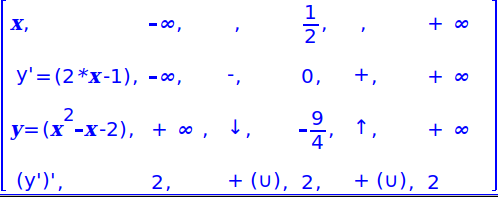
\includegraphics[width=0.75\textwidth]{xcas-tabvar1.png}
\end{center}
\begin{itemize}
  \item The first row, the \texttt{x} row, gives the endpoint of
  subintervals of the domain.  In this case, the subintervals go from
  $-\infty$ to $1/2$ and from $1/2$ to $\infty$.
  \item The second row, the \texttt{y'} row, gives the values of the
  derivative at the values in the first row (or limits, in the case of
  $\pm\infty$), and between them the sign ($+$ or $-$) of the
  derivative in the corresponding subinterval.
  \item The third row, the \texttt{y} row, gives the values of the
  function at the values in the first row, and between them whether
  the function is increasing or decreasing in the corresponding
  subinterval.
  \item The fourth row, the \texttt{y''} 
  row, gives the values of the second derivative at the values in the
  first row, and between them whether the graph is concave up or
  concave down in the subinterval.
\end{itemize}

\noindent
Input:
\begin{center}
  \tt
  tabvar((2*t-1)/(t-1),t)
\end{center}
Output:
\begin{center}
  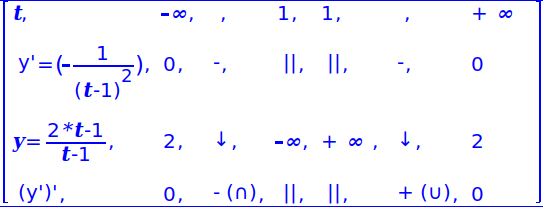
\includegraphics[width=0.75\textwidth]{xcas-tabvar2.png}
\end{center}
Note that in this case, the value 1 appears twice in the first row, so
that both one-sided limits of \texttt{y} can be displayed at the
vertical asymptote $t=1$.  The values of 2 for \texttt{y} at $-\infty$
and $\infty$ indicate a horizontal asymptote of $y=2$.

\section{Derivation and applications.}
\subsection{Functional derivative  : {\tt function\_diff}}\index{function\_diff}
{\tt function\_diff} takes a function as argument.\\
{\tt function\_diff} returns the derivative function of this function.\\
Input :
\begin{center}{\tt function\_diff(sin)}\end{center}
Output :
\begin{center}{\tt (` x`)->cos(` x`)}\end{center}  
Input :
\begin{center}{\tt function\_diff(sin)(x)}\end{center}
Output :
\begin{center}{\tt cos(x)}\end{center}  
Input :
\begin{center}{\tt f(x):=x\verb|^|2+x*cos(x)}\end{center} 
\begin{center}{\tt function\_diff(f)}\end{center}
Output :
\begin{center}{\tt  (` x`)->2*` x`+cos(` x`)+` x`*(-(sin(` x`)))}\end{center}  
Input :
\begin{center}{\tt function\_diff(f)(x)}\end{center}
Output :
\begin{center}{\tt  cos(x)+x*(-(sin(x)))+2*x}\end{center}  
To define the function $g$ as $f'$, input :\\
\begin{center}{\tt g:=function\_diff(f)}\end{center}
The {\tt function\_diff} instruction has the same effect as
using the expression derivative in conjunction with {\tt unapply} :
\begin{center}{\tt g:=unapply(diff(f(x),x),x)}\end{center}
\begin{center}{\tt g(x)}\end{center} 
Output :
\begin{center}{\tt  cos(x)+x*(-(sin(x)))+2*x}\end{center}  
{\bf Warning !!!}\\
In {\tt Maple} mode, for compatibility,
{\tt D} may be used in place of {\tt function\_diff}.
For this reason, it is impossible to assign a variable named 
{\tt D} in {\tt Maple} mode (hence you can not name a 
geometric object {\tt D}).

\subsection{Length of an arc : {\tt arcLen}}\index{arcLen}
\label{sec:arclen}
\noindent {\tt arcLen} takes four arguments : an expression $ex$ (resp. a list
of two expressions $[ex1,ex2]$), the name of a parameter and two values $a$
and $b$ of this parameter.\\
{\tt arcLen} computes the length of the curve define by the equation 
$y=f(x)=ex$ (resp. by $x=ex1,y=ex2$) when the parameter values varies from $a$ 
to $b$, using the formula
{\tt arcLen(f(x),x,a,b)=}\\  
{\tt integrate(sqrt(diff(f(x),x)\verb|^|2+1),x,a,b)}\\
or \\
{\tt integrate(sqrt(diff(x(t),t)\verb|^|2+diff(y(t),t)\verb|^|2),t,a,b)}.\\

{\bf Examples}
\begin{itemize}
\item Compute the length of the parabola $y=x^2$ from $x=0$ to $x=1$.\\
Input :
\begin{center}{\tt arcLen(x\verb|^|2,x,0,1)}\end{center}
or
\begin{center}{\tt arcLen([t,t\verb|^|2],t,0,1)}\end{center}
Output :
\begin{center}{\tt -1/4*log(sqrt(5)-2)-(-(sqrt(5)))/2}\end{center} 
\item Compute the length of the curve $y=\cosh(x)$ from $x=0$ to 
$x=\ln(2)$.\\
Input :
\begin{center}{\tt arcLen(cosh(x),x,0,log(2))}\end{center}
Output :
\begin{center}{\tt 3/4}\end{center}
\item Compute the length of the circle $x=\cos(t),y=\sin(t)$ from $t=0$ to 
$t=2*\pi$.\\
Input :
\begin{center}{\tt arcLen([cos(t),sin(t)],t,0,2*pi)}\end{center}
Output :
\begin{center}{\tt 2*pi}\end{center}
\end{itemize}

Alternatively, the \texttt{arcLen} command can take a single argument of
a geometric curve defined in one of the graphics chapters (chapters
\ref{chap:2dgraphics} and \ref{chap:3dgraphics}).\\
Input:
\begin{center}
  \tt
  arcLen(circle(0,1,0,pi/2))    
\end{center}
Output:
\begin{center}
  \tt
 1/2*pi 
\end{center}
Input:
\begin{center}
  \tt
  arcLen(arc(0,1,pi/2))
\end{center}
Output:
\begin{center}
  \tt
  sqrt(2)/4*pi  
\end{center}

\subsection{Maximum and minimum of an expression: {\tt fMax fMin}}\index{fMax}\index{fMin} 
\noindent{\tt fMax} and {\tt fMin} take one or two arguments : an expression 
of a variable and the name of this variable (by default {\tt x}).\\
{\tt fMax} returns the abscissa 
of a maximum of the expression.\\
{\tt fMin} returns the abscissa 
of a minimum of the expression.\\
Input :
\begin{center}{\tt fMax(sin(x),x)}\end{center}
Or :
\begin{center}{\tt fMax(sin(x))}\end{center}
Or :
\begin{center}{\tt fMax(sin(y),y)}\end{center}
Output :
\begin{center}{\tt pi/2}\end{center} 
Input :
\begin{center}{\tt fMin(sin(x),x)}\end{center}
Or :
\begin{center}{\tt fMin(sin(x))}\end{center}
Or :
\begin{center}{\tt fMin(sin(y),y)}\end{center}
Output :
\begin{center}{\tt -pi/2}\end{center} 
Input :
\begin{center}{\tt fMin(sin(x)\verb|^|2,x)}\end{center}
Output :
\begin{center}{\tt 0}\end{center}

{\tt fMax} and {\tt fMin} can also compute the maximum resp.~minimum of a nonlinear multivariate expression subject to a set of nonlinear equality and/or inequality constraints. Both functions in such cases take four to six arguments:
\begin{itemize}
	\item objective function (an expression)
	\item list of constraints (equalities and inequalities)
	\item list of problem variables
	\item initial guess (must be a list of nonzero reals representing a feasible point)
	\item precision (optional), if not given the default epsilon value is used
	\item maximum number of iterations (optional)
\end{itemize}
The objective function does not need to be differentiable.
Both {\tt fMin} and {\tt fMax} return the optimal solution as a vector. Note that the actual optimal value of the objective is not returned.

Although the initial point is required to be feasible, the algorithm will sometimes succeed even if it is infeasible. Note that the initial value of a variable must not be zero.

For example, input :
\begin{center}
	\tt fMin((x-5)\verb|^|2+y\verb|^|2-25,[y>=x\verb|^|2],[x,y],[1,1])
\end{center}
Output :
\begin{center}
	\tt [1.2347728624961,1.5246640219568]
\end{center}
Input :
\begin{center}
	\tt fMax((x-2)\verb|^|2+(y-1)\verb|^|2,[-.25x\verb|^|2-y\verb|^|2+1>=0,x-2y+1=0],
	[x,y],[.5,.75])
\end{center}
Output :
\begin{center}
	\tt [-1.82287565553,-0.411437827766]
\end{center}

\subsection{Table of values and graph : {\tt tablefunc} and {\tt plotfunc}}\index{tablefunc|textbf}\index{plotfunc}   
{\tt tablefunc} is a special command that should be run from inside
the spreadsheet. It returns the evaluation of an expression $ex$ 
depending on a variable $x$ for $x=x_0,\ x_0+h,....$~:
\begin{center}
{\tt tablefunc(ex,x,x\_0,h)} or {\tt tablefunc(ex,x)}
\end{center}
In the latter case, the default value for ${\tt x_0}$
is the default minimum value of $x$ from the graphic configuration
and the default value for the step $h$ is 0.1 times the difference
between the default maximum and minimum values of $x$ (from the
graphic configuration).\\
Example: type {\tt Alt+t} to open a spreadsheet if none are open.
Then select a cell of the spreadsheet (for example {\tt C0}) and to get
the table of {\tt "sinus"}, input in the command line of the spreadsheet : 
\begin{center}{\tt tablefunc(sin(x),x)}\end{center}
This will fill two columns with the numeric value of {\tt x} and 
{\tt sin(x)} :
\begin{itemize}
\item in the first column the variable {\tt x}, 
the value of the step {\tt h}
(1.0),  the minimum value of $x$ (-5.0), then a formula, for example 
{\tt=C2+C\$1}, and the remaining rows 
of the column is filled by pasting this formula.
\item in the next column the function {\tt sin(x)}, the word
"Tablefunc", a formula, 
for example {\tt =evalf(subst(D\$0,C\$0,C2))}, and the remaining rows
of the column are filled by pasting this formula.
\end{itemize}
Hence the values of {\tt sin(x)} are on the same rows as the values 
of {\tt x}. Note that the step and begin value and the expression 
may be easily changed by modifying the correspondent cell.

The graphic representation may be plotted with the {\tt plotfunc} command 
(see \ref{sec:plotfunc}).

\subsection{Derivative and partial derivative}\index{diff|textbf}\index{derive|textbf}\index{deriver|textbf}
\noindent{\tt diff} or {\tt derive} may have one or two arguments 
to compute a first order derivative (or first order partial
derivative) of an expression or of a list of expressions, 
or several arguments to compute 
the $n$-th partial derivative of an expression or list of expressions.

\subsubsection{Derivative and first order partial derivative : {\tt diff derive deriver}}
{\tt diff} (or {\tt derive}) takes two arguments : an expression and a variable
(resp. a vector of variable names) (see several variable functions in
 \ref{sec:plusvar}). If only one argument is provided, the derivative
is taken with respect to {\tt x}\\
{\tt diff} (or {\tt derive}) returns the derivative (resp. a vector of 
derivatives) of the expression with respect to the variable (resp. with respect 
to each variable) given as second argument.\\
Examples :
\begin{itemize}
\item Compute :
$$\frac {\partial (x y^2 z^3+x y z)}{\partial z}$$
Input :
\begin{center}{\tt  diff(x*y\verb|^|2*z\verb|^|3+x*y*z,z)}\end{center}
Output :
\begin{center}{\tt x*y\verb|^|2*3*z\verb|^|2+x*y}\end{center}
\item Compute the 3 first order partial derivatives of $x*y^2*z^3+x*y*z$.\\
Input :
\begin{center}{\tt  diff(x*y\verb|^|2*z\verb|^|3+x*y,[x,y,z])}\end{center}
Output :
\begin{center}{\tt [y\verb|^|2*z\verb|^|3+y*z, x*2*y*z\verb|^|3+x*z, x*y\verb|^|2*3*z\verb|^|2+x*y]}\end{center}
% \item Compute :
% $$\frac {\partial^3 (x.y^2.z^3+x.y.z)}{\partial y\partial^2 z}$$
% Input :
% \begin{center}{\tt  diff(x*y \verb|^|2*z\verb|^|3+x*y*z,y,z\$2)}\end{center}
% Output :
% \begin{center}{\tt x*2*y*3*2*z}\end{center}
\end{itemize}

\subsubsection{Derivative and $n$-th order
partial derivative : {\tt diff derive deriver}}\index{\$}
\noindent {\tt derive} (or {\tt diff}) may take more than two arguments : an
expression and the names of the derivation variables (each variable
may be followed by \$$n$ to indicate the number $n$ of derivations).\\
{\tt diff} returns the partial derivative of the expression with respect to 
the variables given after the first argument.

The notation \$ is useful if you want to derive $k$ times with
respect to the same variable, instead of entering $k$ times the
same variable name, one enters the variable name followed by {\tt \$k},
for example {\tt x\$3} instead of {\tt(x,x,x)}. 
Each variable may be followed by a \$, for example 
{\tt diff(exp(x*y),x\$3,y\$2,z)} is the same as 
{\tt diff(exp(x*y),x,x,x,y,y,z)}\\
{\bf Examples}
\begin{itemize}
\item Compute :
$$\frac {\partial^2 (x y^2 z^3+x y z)}{\partial x\partial z}$$
Input :
\begin{center}{\tt diff(x*y\verb|^|2*z\verb|^|3+x*y*z,x,z)}\end{center}
Output  :
\begin{center}{\tt y\verb|^|2*3*z\verb|^|2+y}\end{center}
\item Compute :
$$\frac {\partial^3 (x y^2 z^3+x y z)}{\partial x\partial^2 z}$$
Input :
\begin{center}{\tt  diff(x*y\verb|^|2*z\verb|^|3+x*y*z,x,z,z)}\end{center}
or :
\begin{center}{\tt  diff(x*y\verb|^|2*z\verb|^|3+x*y*z,x,z\$2)}\end{center}
Output  :
\begin{center}{\tt y\verb|^|2*3*2*z}\end{center}
\item Compute the third derivative of :
$$\frac{1}{x^2+2}$$
Input :
\begin{center}{\tt  normal(diff((1)/(x\verb|^|2+2),x,x,x))}\end{center}
or :
\begin{center}{\tt  normal(diff((1)/(x\verb|^|2+2),x\$3))}\end{center}
Output  :
\begin{center}{\tt (-24*x\verb|^|3+48*x)/(x\verb|^|8+8*x\verb|^|6+24*x\verb|^|4+32*x\verb|^|2+16)}\end{center}
\end{itemize}
{\bf Remark}
\begin{itemize}
\item 
Note the difference between {\tt diff(f,x,y)} and {\tt  diff(f,[x,y])} :\\
{\tt diff}$(f,x,y)$ returns $\displaystyle \frac{\partial^2(f)}{\partial x\partial y}$ and\\
{\tt diff}$(f,[x,y])$ returns
$\displaystyle[\frac{\partial(f)}{\partial x},\frac{\partial
  (f)}{\partial y}]$ 
\item Never define a derivative function with {\tt
    f1(x):=diff(f(x),x)}.
Indeed, {\tt x} would mean two different things Xcas is unable to
deal with: the variable name to
define the $f_1$ function and the differentiation variable.
The right way to define a derivative is either with {\tt
  function\_diff} or:
\begin{center}
{\tt f1:=unapply(diff(f(x),x),x)}
\end{center}
\end{itemize}

\subsection{Implicit differentiation : {\tt implicitdiff}}\index{implicitdiff}
{\tt implicitdiff} is called with one of the following three sets of parameters :
\begin{enumerate}
\item {\tt expr}, {\tt constr}, {\tt depvars}, {\tt diffvars}
\item {\tt constr}, {\tt [depvars]}, {\tt y}, {\tt diffvars}
\item {\tt expr}, {\tt constr}, {\tt vars}, {\tt order=k}, {\tt [pt]}
\end{enumerate}
Details on parameters :
\begin{itemize}
\item {\tt expr} : differentiable expression $ f(x_1,x_2,\dots,x_n,y_1,y_2,\dots,y_m) $
\item {\tt constr} : (list of) equality constraint(s) $ g_i(x_1,\dots,x_n,y_1,\dots,y_m)=0 $ or vanishing expression(s) $ g_i $, where $ i=1,2,\dots,m $
\item {\tt depvars} : (list of) dependent variable(s) $ y_1,y_2,\dots,y_m $, each of which may be entered as a symbol, e.g.~{\tt yi}, or a function of independent variable(s), e.g.~{\tt yi(x1,x2,..,xn)}
\item {\tt diffvars} : sequence of variables $ x_{i_1},x_{i_2},\dots,x_{i_k} $ with respect to which is {\tt expr} differentiated
\item {\tt vars} : independent and dependent variables entered as symbols in single list such that dependent variables come last, e.g.~{\tt [x1,..,xn,y1,..,ym]}
\item {\tt y} : (list of) dependent variable(s) $ y_{j_1},y_{j_2},\dots,y_{j_l} $ that need to be differentiated
\end{itemize}
Dependent variables $ y_1,y_2,\dots,y_m $ are implicitly defined with $ m $ constraints in {\tt constr}. By implicit function theorem, the Jacobian matrix of $ \mathbf{g}=(g_1,g_2,\dots,g_m) $ has to be full rank.

When calling {\tt implicitdiff}, first two sets of parameters are used when specific partial derivative is needed. In the first case, {\tt expr} is differentiated with respect to {\tt diffvars}.

\noindent Input :
\begin{center}
{\tt implicitdiff(x*y,-2x\verb|^|3+15x\verb|^|2*y+11y\verb|^|3-24y=0,y(x),x)}
\end{center}
Output :
\begin{center}
{\tt (2*x\verb|^|3-5*x\verb|^|2*y+11*y\verb|^|3-8*y)/(5*x\verb|^|2+11*y\verb|^|2-8)}
\end{center}
In the second case (elements of) {\tt y} is differentiated. If {\tt y} is a list of symbols, a list containing their derivatives will be returned. The following examples compute $ \frac{\mathrm{d}\,y}{\mathrm{d}\,x} $.\\
Input :
\begin{center}
{\tt implicitdiff(x\verb|^|2*y+y\verb|^|2=1,y,x)}
\end{center}
Output :
\begin{center}
{\tt -2*x*y/(x\verb|^|2+2*y)}
\end{center}
Input :
\begin{center}
{\tt implicitdiff([x\verb|^|2+y=z,x+y*z=1],[y(x),z(x)],y,x)}
\end{center}
Output :
\begin{center}
{\tt (-2*x*y-1)/(y+z)}
\end{center}
In the next example, $ \frac{\mathrm{d}\,y}{\mathrm{d}\,x} $ and $ \frac{\mathrm{d}\,z}{\mathrm{d}\,x} $ are computed.\\
Input :
\begin{center}
{\tt implicitdiff([-2x*z+y\verb|^|2=1,x\verb|^|2-exp(x*z)=y],}\\
{\tt [y(x),z(x)],[y,z],x)}
\end{center}
Output :
\begin{center}
{\tt [2*x/(y*exp(x*z)+1),}\\
{\tt (2*x*y-y*z*exp(x*z)-z)/(x*y*exp(x*z)+x)]}
\end{center}

For the third case of input syntax, all partial derivatives of order equal to {\tt order}, i.e.~$ k $, are computed. If $ k=1 $ they are returned in a single list, which represents the gradient of {\tt expr} with respect to independent variables. For $ k=2 $ the corresponding hessian matrix is returned. When $ k>2 $, a table with keys in form {\tt [k1,k2,..,kn]}, where $ \sum_{i=1}^nk_i=k $, is returned. Such key corresponds to \[ \frac{\partial^k f}{\partial x_1^{k_1}\,\partial x_2^{k_2}\,\cdots\,\partial x_n^{k_n}}. \]
Input :
\begin{center}
{\tt f:=x*y*z; g:=-2x\verb|^|3+15x\verb|^|2*y+11y\verb|^|3-24y=0;}\\
{\tt implicitdiff(f,g,[x,z,y],order=1)}
\end{center}
Output :
\begin{center}
{\tt [(2*x\verb|^|3*z-5*x\verb|^|2*y*z+11*y\verb|^|3*z-8*y*z)/(5*x\verb|^|2+11*y\verb|^|2-8),}\\
{\tt x*y]}
\end{center}
Input :
\begin{center}
{\tt implicitdiff(f,g,order=2,[1,-1,0])}
\end{center}
Output :
\begin{center}
{\tt [[64/9,-2/3],[-2/3,0]]}
\end{center}
In the next example, the value of $ \frac{\partial^4 f}{\partial x^4} $ is computed at point $ (x=0,y=0,z) $.\\
Input :
\begin{center}
{\tt pd:=implicitdiff(f,g,[x,z,y],order=4,[0,z,0]);}\\
{\tt pd[4,0]}
\end{center}
Output :
\begin{center}
{\tt -2*z}
\end{center}

\subsection{Numerical differentiation : {\tt numdiff}}\index{numdiff}
{\tt numdiff} takes three mandatory arguments: lists $X=\{\alpha_0,\alpha_1,\dots,\alpha_n\}$, $Y=\{\beta_0,\beta_1,\dots,\beta_n\}$ of real numbers, where $n\geq 1$, and a real number $x_0$. The optional fourth argument is an integer $m$, which defaults to 1. The function returns an approximation of the $m$-th derivative of function $f$, given by $f(\alpha_k)=\beta_k$, $k=0,1,\dots,n$, at point $x_0$.

The strategy is to use Fornberg's algorithm described in ``Generation of Finite Difference Formulas on Arbitrarily Spaced Grids'', {\it Mathematics of Computation}, 51(184):699--706, 1988. The complexity of this algorithm is $O(n^2m)$ in both time and space. To avoid numerical instability, {\tt numdiff} operates in exact arithmetic. Unless a symbolic variable is present in the input, the result is returned using the floating-point representation.

Note that $\alpha_0,\alpha_1,\dots,\alpha_n$ do not have to be equally spaced, but they must be mutually different and input in ascending order. There are no restrictions on the choice of $x_0$.

For example, let $f(x)=\sin(x)\mathrm{e}^{-x}$, $x\in[0,1]$. We sample this function at points
\[ X=[0,0.1,0.2,0.4,0.5,0.7,0.8,1] \]
by computing the list $Y=f(X)$. Input :
\begin{center}
  \tt f:=unapply(sin(x)*exp(-x),x)\\X:=[0,0.1,0.2,0.4,0.5,0.7,0.8,1]; Y=apply(f,X)
\end{center}
Now we approximate the second derivative at the point $x_0=\frac{1}{\pi}$. Input :
\begin{center}
  \tt x0:=1/pi:; d:=numdiff(X,Y,x0,2)
\end{center}
Finally, we compute the relative error of the obtained approximation. Input :
\begin{center}
  \tt abs(d-f''(x0))/abs(f''(x0))*100
\end{center}
Output :
\begin{center}
  \tt 2.82983388966e-05
\end{center}
The result is expressed in percentages.

Optionally, a sequence of values of the parameter $m$ may be passed to {\tt numdiff}. In that case the function returns the list of approximations of the respective derivatives at $x_0$. This is faster than calling {\tt numdiff} to approximate one derivative at a time. For example, let us approximate the zeroth, first and second derivative of the function
\[ f(x)=1-\frac{1}{1+x^2},\quad x\in[0,1], \]
at point $x_0=\gamma$, where $\gamma\approx 0.57722$ is Euler-Mascheroni constant, by sampling $f$ at 21 equidistant points in the segment $[0,1]$. Input :
\begin{center}
	\tt f:=unapply(1-1/(1+x\verb|^|2),x)\\
	X:=[(0.05*k)\$(k=0..20)]:; Y:=apply(f,X):;\\
	numdiff(X,Y,euler\_gamma,0,1,2)
\end{center}
Output :
\begin{center}
	\tt [0.249912571952,0.649519026355,0.000393517939481]
\end{center}
The correct values are $f(\gamma)=0.249912571952$, $f'(\gamma)=0.649519026356$ and $f''(\gamma)=0.000393517946748$.

{\tt numdiff} can be used for generating custom finite-difference stencils for approximation of derivatives. For example, let $X=[-1,0,2,4]$, $Y=[a,b,c,d]$ and $x_0=1$. To obtain an approximation formula for the second derivative, input :
\begin{center}
	\tt numdiff([-1,0,2,4],[a,b,c,d],1,2)
\end{center}
Output :
\begin{center}
	\tt 2*a/5-b/2+d/10
\end{center}
The approximation is always a linear combination of elements in $Y$, regardless of $X$, $x_0$ and $m$.

Given $X$ and $Y$, the Lagrange polynomial passing through points $(\alpha_k,\beta_k)$ where $k=0,1,\dots,n$ can be obtained by setting $m=0$ and entering a symbol for $x_0$. For example, letting $X=[-2,0,1]$ and $Y=[2,4,1]$ input :
\begin{center}
	\tt expand(numdiff([-2,0,1],[2,4,1],x,0))
\end{center}
Output :
\begin{center}
	\tt -4*x\verb|^|2/3-5*x/3+4
\end{center}
The same result is obtained by entering {\tt lagrange([-2,0,1],[2,4,1],x)}.

\section{Integration}
\subsection{Antiderivative and definite integral : {\tt integrate int Int}}\index{integrate}\index{Int}\index{int}
\noindent{\tt integrate} (or {\tt int}) computes a primitive
or a definite integral. A difference between the two 
commands is that if you input {\tt quest()} just after the evaluation of 
{\tt  integrate}, the answer is written with the $\int$ symbol.

{\tt integrate} (or {\tt int} or {\tt Int}) takes one, two or four arguments.
\begin{itemize}
\item with one or two arguments\\
an expression or an expression and 
the name of a variable (by default {\tt x}),\\
{\tt integrate} (or {\tt int}) returns a primitive of the expression with 
respect to the  variable given as second argument.\\
Input :
\begin{center}{\tt integrate(x\verb|^|2)}\end{center}
Output  :
\begin{center}{\tt x\verb|^|3/3}\end{center}
Input :
\begin{center}{\tt integrate(t\verb|^|2,t)}\end{center}
Output  :
\begin{center}{\tt t\verb|^|3/3}\end{center}
\item with four arguments :\\
an expression, a name of a variable and the bounds of the definite integral,\\ 
{\tt integrate} (or {\tt int}) returns the exact
value of the definite integral if the computation was successful or
an unevaluated integral otherwise.\\
Input :
\begin{center}{\tt integrate(x\verb|^|2,x,1,2)}\end{center}
Output  :
\begin{center}{\tt 7/3}\end{center}
Input :
\begin{center}{\tt integrate(1/(sin(x)+2),x,0,2*pi)}\end{center}
Output  after simplification (with the {\tt simplify} command) :
\begin{center}{\tt 2*pi*sqrt(3)/3}\end{center}
\end{itemize}


{\tt Int} is the inert form of {\tt integrate}, it prevents evaluation
for example to avoid a symbolic computation that might not be
successful if you just want a numeric
evaluation.\\
Input :
\begin{center}{\tt evalf(Int(exp(x\verb|^|2),x,0,1))}\end{center}
or :
\begin{center}{\tt evalf(int(exp(x\verb|^|2),x,0,1))}\end{center}
Output  :
\begin{center}{\tt 1.46265174591}\end{center}

{\bf Exercise 1}\\
Let $$f(x)=\frac {x}{x^2-1}+\ln(\frac {x+1}{x-1})$$
Find a primitive of $f$.\\
Input :
\begin{center}{\tt int(x/(x\verb|^|2-1)+ln((x+1)/(x-1)))}\end{center}
Output : 
\begin{center}{\tt x*log((x+1)/(x-1))+log(x\verb|^|2-1)+1/2*log(2*x\verb|^|2/2-1)}\end{center}
Or define the function {\tt f}, input :
\begin{center}{\tt f(x):=x/(x\verb|^|2-1)+ln((x+1)/(x-1))}\end{center}
then input :
\begin{center}{\tt int(f(x))}\end{center}
Output of course the same result.\\
{\bf Warning}\\
For {\tt Xcas}, {\tt log} is the natural logarithm (like {\tt ln}),
as {\tt log10} is 10-basis logarithm

{\bf Exercise 2}\\
Compute :
$$\int \frac {2}{x^6+2 \cdot x^4+x^2} \ dx $$
Input :
\begin{center}{\tt int(2/(x\verb|^|6+2*x\verb|^|4+x\verb|^|2))}\end{center}
Output :
\begin{center}{\tt 2*((3*x\verb|^|2+2)/(-(2*(x\verb|^|3+x)))+-3/2*atan(x))}\end{center}

{\bf Exercise 3}\\
Compute :
$$\int \frac {1}{\sin(x)+\sin(2 \cdot x )} \ dx $$
Input :
\begin{center}{\tt integrate(1/(sin(x)+sin(2*x )))}\end{center}
Output :
\begin{center}{\tt (1/-3*log((tan(x/2))\verb|^|2-3)+1/12*log((tan(x/2))\verb|^|2))*2}\end{center} 

\subsection{Primitive and definite integral : {\tt risch}}\index{risch}

\noindent
The {\tt risch} command takes one mandatory argument and three
optional arguments.  The first argument is an expression to be
integrated.  If the variable is not \texttt{x}, then the second
argument is the variable.  The third and fourth arguments are the
limits of integration for when you want a definite integral.\\
\texttt{risch} returns a primitive (with one or two arguments) or a
definite integral (with four arguments).\\
Input:
\begin{center}{\tt risch(x\verb|^|2)}\end{center}
Output:
\begin{center}{\tt x\verb|^|3/3}\end{center}
Input:
\begin{center}{\tt risch(x\verb|^|2,x,0,1)}\end{center}
Output:
\begin{center}{\tt 1/3}\end{center}
Input:
\begin{center}{\tt risch(t\verb|^|2,t)}\end{center}
Output:
\begin{center}{\tt t\verb|^|3/3}\end{center}
Input :
\begin{center}{\tt risch(exp(-x\verb|^|2))}\end{center}
Output  :
\begin{center}{\tt integrate(exp(x\verb|^|2),x)}\end{center}
that is to say that $\exp(-x^2)$ has no primitive expressed
with usual functions.

\subsection{Discrete summation: {\tt sum}}\index{sum|textbf}
\noindent{\tt sum} takes two or four arguments :
\begin{itemize}
\item four arguments\\
an expression, the name of the variable (for 
example {\tt n}), and the bounds (for example {\tt a} and {\tt b}).\\
{\tt sum} returns the discrete sum of this expression with respect to
the variable from $a$ to $b$.\\
Input :
\begin{center}{\tt sum(1,k,-2,n) }\end{center}
Output  :
\begin{center}{\tt n+1+2}\end{center}
Input :
\begin{center}{\tt normal(sum(2*k-1,k,1,n))}\end{center}
Output  :
\begin{center}{\tt n\verb|^|2}\end{center}
Input :
\begin{center}{\tt sum(1/(n\verb|^|2),n,1,10)}\end{center}
Output  :
\begin{center}{\tt 1968329/1270080}\end{center} 
Input :
\begin{center}{\tt sum(1/(n\verb|^|2),n,1,+(infinity)) }\end{center}
Output  :
\begin{center}{\tt pi\verb|^|2/6}\end{center}
Input :
\begin{center}{\tt sum(1/(n\verb|^|3-n),n,2,10) }\end{center}
Output  :
\begin{center}{\tt 27/110}\end{center} 
Input :
\begin{center}{\tt sum(1/(n\verb|^|3-n),n,1,+(infinity)) }\end{center}
Output  :
\begin{center}{\tt 1/4}\end{center}
This result comes from the decomposition of ${\tt 1/(n\verb|^|3-n)}$.\\
Input :
\begin{center}{\tt partfrac(1/(n\verb|^|3-n)) }\end{center}
Output  :
\begin{center}{\tt 1/(2*(n+1))-1/n+1/(2*(n-1))}\end{center}
Hence :\\
$\displaystyle \sum_{n=2}^N -\frac{1}{n}=-\sum_{n=1}^{N-1} \frac{1}{n+1}=-\frac{1}{2}-\sum_{n=2}^{N-2} \frac{1}{n+1}-\frac{1}{N}$\\
$\displaystyle \frac{1}{2}*\sum_{n=2}^N \frac{1}{n-1}=\frac{1}{2}*(\sum_{n=0}^{N-2} \frac{1}{n+1})=\frac{1}{2}*(1+\frac{1}{2}+\sum_{n=2}^{N-2}\frac{1}{n+1})$\\
$\displaystyle \frac{1}{2}*\sum_{n=2}^N \frac{1}{n+1}=\frac{1}{2}*(\sum_{n=2}^{N-2} \frac{1}{n+1}+\frac{1}{N}+\frac{1}{N+1})$\\
After simplification by $\sum_{n=2}^{N-2}$, it remains :\\
 $\displaystyle -\frac{1}{2}+\frac{1}{2}*(1+\frac{1}{2})-\frac{1}{N}+\frac{1}{2}*(\frac{1}{N}+\frac{1}{N+1})=\frac{1}{4}-\frac{1}{2N(N+1)}$\\
Therefore :
\begin{itemize}
\item for $N=10$ the sum is equal to : $1/4-1/220=27/110$
\item for $N=+\infty$ the sum is equal to : $1/4$ because $\frac{1}{2N(N+1)}$ 
approaches zero when $N$ approaches infinity.
\end{itemize}

\item two arguments \\
an expression of one variable (for example $f$) and the name of this
 variable (for example $x$).\\
{\tt sum} returns the discrete antiderivative of this expression, i.e. 
an expression $G$ such that $G_{|x=n+1}-G_{|x=n}=f_{|x=n}$.\\ 
Input :
\begin{center}{\tt sum(1/(x*(x+1)),x)}\end{center}
Output  :
\begin{center}{\tt -1/x}\end{center}
\end{itemize}

\subsection{Riemann sum : {\tt sum\_riemann}}\index{sum\_riemann}
\noindent{\tt sum\_riemann} takes two arguments : an expression depending on 
two variables and the list of the name of these two variables.\\ 
{\tt sum\_riemann(expression(n,k),[n,k])} returns in the neighborhood of
 $ n=+\infty$ an equivalent of $\sum_{k=1}^n expression(n,k)$ (or of
$ \sum_{k=0}^{n-1} expression(n,k)$ or of $ \sum_{k=1}^{n-1} expression(n,k)$) 
when the sum is looked on as a Riemann sum associated to a continuous 
function defined on [0,1] or returns  
{\tt "it is probably not a Riemann sum"} when the no result is found.\\
{\bf Exercise 1}\\
Suppose $\displaystyle S_n=\sum_{k=1}^n \frac{k^2}{n^3}$.\\
Compute $\displaystyle \lim_{n \rightarrow  +\infty} S_n$.\\
Input :
\begin{center}{\tt sum\_riemann(k\verb|^|2/n\verb|^|3,[n,k])}\end{center}
Output  :
\begin{center}{\tt 1/3}\end{center}
{\bf Exercise 2}\\
Suppose $\displaystyle S_n=\sum_{k=1}^n \frac{k^3}{n^4}$.\\
Compute $\displaystyle \lim_{n \rightarrow  +\infty} S_n$.\\
Input :
\begin{center}{\tt sum\_riemann(k\verb|^|3/n\verb|^|4,[n,k])}\end{center}
Output  :
\begin{center}{\tt 1/4}\end{center}
{\bf Exercise 3}\\
Compute 
$\displaystyle \lim_{n \rightarrow  +\infty}(\frac{1}{n+1}+\frac{1}{n+2}+...+\frac{1}{n+n})$.\\
Input :
\begin{center}{\tt sum\_riemann(1/(n+k),[n,k])}\end{center}
Output :
\begin{center}{\tt log(2)}\end{center}
{\bf Exercise 4}\\
Suppose $\displaystyle S_n=\sum_{k=1}^n \frac{32n^3}{16n^4-k^4}$.\\
Compute $\displaystyle \lim_{n \rightarrow  +\infty} S_n$.\\
Input :
\begin{center}{\tt sum\_riemann(32*n\verb|^|3/(16*n\verb|^|4-k\verb|^|4),[n,k])}\end{center}
Output :
\begin{center}{\tt 2*atan(1/2)+log(3)}\end{center}

\subsection{Integration by parts : {\tt ibpdv} and {\tt ibpu}}
\subsubsection{\tt ibpdv}\index{ibpdv}
\noindent{\tt ibpdv} is used to search the primitive of an expression written 
as $u(x).v'(x)$.\\
{\tt ibpdv} takes two arguments :
\begin{itemize}
\item an expression 
 $u(x) * v'(x)$ and $v(x)$ (or a list of two expressions 
$[F(x), u(x)*v'(x)]$ and $v(x)$),
\item or an expression $g(x)$ and $0$ (or a list of two expressions 
$[F(x), g(x)]$ and $0$).
\end{itemize}
{\tt ibpdv} returns :
\begin{itemize}
\item if $v(x) \neq 0$, the list $[u(x) v(x),-v(x) u'(x)]$ (or 
$[F(x)+u(x) v(x),-v(x) u'(x)]$),
\item if the second argument is zero, a primitive of the first argument 
$g(x)$ (or $F(x)$+a primitive of $g(x)$) :\\
hence, {\tt ibpdv(g(x),0)} returns a primitive {\tt G(x)} of {\tt g(x)} or \\
{\tt ibpdv([F(x),g(x)],0)} returns {\tt F(x)+G(x)} where {\tt diff(G(x))=g(x)}.
\end{itemize}
Hence, {\tt ibpdv} returns the terms computed in an integration by parts, 
with the possibility of doing several {\tt ibpdv}s successively.\\
When the answer of {\tt ibpdv(u(x)*v'(x),v(x))} is computed, to obtain a 
primitive of $u(x) v'(x)$, it remains to 
compute the integral of the second term of this answer and then, to sum this 
integral with the first term of this answer : to do this, just use  
{\tt ibpdv} command with the answer as first argument and  
a new $v(x)$ (or $0$ to terminate the integration) as second argument.\\ 
Input :
\begin{center}{\tt ibpdv(ln(x),x) }\end{center}
Output :
\begin{center}{\tt [x ln(x),-1]}\end{center}
then
\begin{center}{\tt ibpdv([x ln(x),-1],0) }\end{center}
Output :
\begin{center}{\tt -x+x ln(x)}\end{center}
{\bf Remark}\\
 When the first argument of {\tt ibpdv} is a list of two elements, {\tt ibpdv} 
works only on the last element of this list and adds the integrated term to
the first element of this list.  
(therefore it is possible to do several {\tt ibpdv}s successively).\\
For example :\\
{\tt ibpdv((log(x))\verb|^|2,x) = [x*(log(x))\verb|^|2,-(2*log(x))]}\\ 
it remains to integrate {\tt -(2*log(x))}, the input :\\
{\tt ibpdv(ans(),x)} or input :\\
{\tt ibpdv([x*(log(x))\verb|^|2,-(2*log(x))],x)}\\
Output :\\
{\tt [x*(log(x))\verb|^|2+x*(-(2*log(x))),2]}\\
and it remains to integrate {\tt 2}, hence input {\tt ibpdv(ans(),0)} or\\
{\tt ibpdv([x*(log(x))\verb|^|2+x*(-(2*log(x))),2],0)}.\\
Output :
{\tt x*(log(x))\verb|^|2+x*(-(2*log(x)))+2*x}
\subsubsection{\tt ibpu}\index{ibpu}
\noindent{\tt ibpu} is used to search the primitive of an expression written 
as $u(x).v'(x)$
{\tt ibpu} takes two arguments  : 
\begin{itemize}
\item an expression $u(x)*v'(x)$ and $u(x)$ (or a list of two expressions 
$[F(x), u(x)*v'(x)]$ and $u(x)$),
\item an expression $g(x)$ and $0$ (or a list of two expressions $[F(x), g(x)]$ 
and $0$).
\end{itemize}
{\tt ibpu} returns :
\begin{itemize}
\item if $u(x) \neq 0$, the list $[u(x)*v(x),-v(x)*u'(x)]$ 
(or returns the list $[F(x)+u(x)*v(x),-v(x)*u'(x)]$),
\item if the second  argument is zero, a primitive of the first argument $g(x)$
(or $F(x)$+a primitive of $g(x)$):\\ 
{\tt ibpu(g(x),0)} returns {\tt G(x)} where {\tt diff(G(x))=g(x)} or\\
 {\tt ibpu([F(x),g(x)],0)} returns {\tt F(x)+G(x)} where {\tt diff(G(x))=g(x)}.
\end{itemize}
Hence, {\tt ibpu} returns the terms computed in an integration by parts, 
with the possibility of doing several {\tt ibpu}s successively.\\
When the answer of {\tt ibpu(u(x)*v'(x),u(x))} is computed, to obtain a 
primitive of $u(x) v'(x)$, it remains to 
compute the integral of the second term of this answer and then, to sum this 
integral with the first term of this answer : to do this, just use  
{\tt ibpu} command with the answer as first argument and  
a new $u(x)$ (or $0$ to terminate the integration) as second argument.\\ 
Input :
\begin{center}{\tt ibpu(ln(x),ln(x)) }\end{center}
Output :
\begin{center}{\tt [x*ln(x),-1]}\end{center}
then
\begin{center}{\tt ibpu([x*ln(x),-1],0) }\end{center}
Output :
\begin{center}{\tt -x+x*ln(x)}\end{center}
{\bf Remark}\\
When the first argument of {\tt ibpu} is a list of two elements, {\tt ibpu} 
works only on the last element of this list and adds the integrated term to
the first element of this list.  
(therefore it is possible to do several {\tt ibpu}s successively).\\
For example :\\
{\tt ibpu((log(x))\verb|^|2,log(x)) = [x*(log(x))\verb|^|2,-(2*log(x))]}\\ 
it remains to integrate {\tt -(2*log(x))}, hence input : \\
{\tt ibpu(ans(),log(x))}
 or input :\\
{\tt ibpu([x*(log(x))\verb|^|2,-(2*log(x))],log(x))}\\
Output :\\
{\tt [x*(log(x))\verb|^|2+x*(-(2*log(x))),2]}\\
it remains to integrate  {\tt 2}, hence input :\\
{\tt ibpu(ans(),0)} or input :\\
{\tt ibpu([x*(log(x))\verb|^|2+x*(-(2*log(x))),2],0)}.\\
Output :
{\tt x*(log(x))\verb|^|2+x*(-(2*log(x)))+2*x}

\subsection{Change of variables : {\tt subst}}
See the {\tt subst} command  in the section \ref{sec:subst}.

\section{Calculus of variations}

\subsection{Determining whether a function is convex : {\tt convex\index{convex}}}
{\tt convex} takes two mandatory arguments, an at least twice differentiable function(al) $f:\mathbb{R}^n\to\mathbb{R}$ and a variable or list of variables. Some variables may depend on a common independent parameter, say $t$, when entered as e.g.~$x(t)$ instead of $x$. The first derivatives of such variables, when encountered in $f$, are treated as independent parameters of $f$.

The command returns a condition or list of conditions under which $f$ is convex. If $f$ is convex on the entire domain, the return value is {\tt true}. If it is nowhere convex, the return value is {\tt false}. Otherwise, the conditions are returned as inequalities which depend on the parameters of $f$. The returned inequalities are not necessarily independent.

An optional third argument {\tt simplify=false} or {\tt simplify=true} may be given. By default is {\tt simplify=true}, which means that simplification is applied when generating convexity conditions. If {\tt simplify=false}, only rational normalization is performed (using the {\tt ratnormal} command).

The command operates by computing the Hessian $H_f$ of $f$ and its principal minors (in total $2^n$ of them where $n$ is the number of parameters) and checks their signs. If all minors are nonnegative, then $H_f$ is positive semidefinite and $f$ is therefore convex.

The function $f$ is said to be \emph{concave} if the function $g=-f$ is convex.

For example, input :
\begin{center}
  \tt convex(3*exp(x)+5x\verb|^|4-ln(x),x)
\end{center}
Output :
\begin{center}
  \tt true
\end{center}
Input :
\begin{center}
  \tt convex(x\verb|^|2+y\verb|^|2+3z\verb|^|2-x*y+2x*z+y*z,[x,y,z])
\end{center}
Output :
\begin{center}
  \tt true
\end{center}
Input :
\begin{center}
  \tt convex(x1\verb|^|3+2x1\verb|^|2+2*x1*x2+x2\verb|^|2/2-8x1-2x2-8,[x1,x2])
\end{center}
Output :
\begin{center}
  \tt [(3*x1+2)>=0,x1>=0]
\end{center}
In the example below, the function $f(x,y,z)=x^2+x\,z+a\,y\,z+z^2$ is not convex regardless of the value $a\in\mathbb{R}$ :
\begin{center}
  \tt convex(x\verb|^|2+x*z+a*y*z+z\verb|^|2,[x,y,z])
\end{center}
Output :
\begin{center}
  \tt false
\end{center}
In the next example we find all values $a\in\mathbb{R}$ for which the function \[f(x,y,z)=x^2+2\,y^2+a\,z^2-2\,x\,y+2\,x\,z-6\,y\,z\] is convex on $\mathbb{R}^3$. Input :
\begin{center}
  \tt cond:=convex(x\verb|^|2+2y\verb|^|2+a*z\verb|^|2-2x*y+2x*z-6y*z,[x,y,z])
\end{center}
Output :
\begin{center}
  \tt [a>=0,(a-1)>=0,(2*a-9)>=0,(a-5)>=0]
\end{center}
The returned inequalities are simplified by {\tt solve} :
\begin{center}
  \tt solve(cond,a)
\end{center}
Output :
\begin{center}
  \tt list[a>=5]
\end{center}
Therefore $f$ is convex for $a\geq 5$.

Let's find the set $S\subset\mathbb{R}^2$ on which the function $f:\mathbb{R}^2\to\mathbb{R}$ defined by
\[ f(x_1,x_2)=\exp(x_1)+\exp(x_2)+x_1\,x_2 \]
is convex. Input :
\begin{center}
  \tt cond:=convex(exp(x1)+exp(x2)+x1*x2,[x1,x2]
\end{center}
Output :
\begin{center}
  \tt (exp(x1)*exp(x2)-1)>=0
\end{center}
Input :
\begin{center}
  \tt lin(cond)
\end{center}
Output :
\begin{center}
  \tt (exp(x1+x2)-1)>=0
\end{center}
From here we conclude that $f$ is convex when $x_1+x_2\geq 0$. The sought set $S$ is therefore the half-space defined by this inequality.

The algorithm respects the assumptions that may be set upon variables. Therefore, the convexity of a given function can be checked only on a particular domain. For example, input :
\begin{center}
  \tt assume(x1>0),assume(x2>0):; convex(exp(x1)+exp(x2)+x1*x2,[x1,x2]
\end{center}
Output :
\begin{center}
  \tt true
\end{center}
Input :
\begin{center}
  \tt assume(x>=0 and x<=pi/4):; convex(exp(y)*sec(x)\verb|^|3-z,[x,y,z])
\end{center}
Output :
\begin{center}
  \tt true
\end{center}

\paragraph{\label{brachistochrone}The Brachistochrone Problem.}
We want to minimize the objective functional \[T(y)=\int_0^{x_1}L(t,y(t),y'(t))\,\mathrm{d} t\] where the Lagrangian $L$ is defined by
\[ L(t,y(t),y'(t))=\sqrt{\frac{1+y'(t)^2}{2\,g\,y(t)}} \]
for $y:[0,x_1]\to\mathbb{R}$ such that $y(0)=y_0$ and $y(x_1)=0$ where $x_1>0$ and $y_0>0$ are fixed (the constant $g$ is the gravitational acceleration). This is called the \emph{brachistochrone problem} (the problem of shortest travel by own weight from the point $(0,y_0)$ to $(x_1,0)$).
By solving Euler-Lagrange equation one obtains a cycloid $\overline{y}(t)$ as the only stationary function for $L$. The problem is to prove that it minimizes $T$, which would be easy if the integrand $L$ was convex. However, it's not the case here :
\begin{center}
  \tt assume(y>=0):; assume(g>0):; convex(sqrt((1+y'\verb|^|2)/(2*g*y)),y(t))
\end{center}
Output :
\begin{center}
  \tt (-diff(y(t),t)\verb|^|2+3)>=0
\end{center}
This is equivalent to $|y'(t)|\leq\sqrt{3}$, which is certainly not satisfied by the cycloid $\overline{y}$ near the point $x=0$.

Using the substitution $y(t)=z(t)^2/2$ we obtain $y'(t)=z'(t)\,z(t)$ and
\[ L(t,y(t),y'(t))=P(t,z(t),z'(t))=\sqrt{\frac{z(t)^{-2}+z'(t)^2}{g}}. \]
The function $P$ is convex :
\begin{center}
  \tt assume(z>=0):; convex(sqrt((z\verb|^|-2+z'\verb|^|2)/g),z(t))
\end{center}
Output :
\begin{center}
  \tt true
\end{center}
Hence the function $\overline{z}(t)=\sqrt{2\,\overline{y}(t)}$, stationary for $P$ (which is verified directly), minimizes the objective functional \[U(z)=\int_0^{x_1}P(t,z(t),z'(t))\,\mathrm{d} t.\] From here and $U(z)=T(y)$ it easily follows that $\overline{y}$ minimizes $T$ and therefore the brachistochrone. For details see John L.~Troutman, \emph{Variational Calculus and Optimal Control} (second edition), page 257.

\subsection{Euler-Lagrange equation(s) : {\tt euler\_lagrange\index{euler\_lagrange}}}
{\tt euler\_lagrange} takes from one to three arguments :
\begin{itemize}
  \item expression $f(x,y,y')$,
  \item independent variable (optional, by default $x$),
  \item dependent variable (optional, by default $y$).
\end{itemize}
If $y\in\mathbb{R}^n$ is required (by default $n=1$), one can enter $y=(y_1,y_2,\dots,y_n)$ as a vector $[y_1,y_2,\dots,y_n]$. In that case, $y':=(y_1',y_2',\dots,y_n')$. Alternatively, one can specify two arguments, $f$ and either $y(x)$ or $[y_1(x),y_2(x),\dots,y_n(x)]$.

The return value is a system of differential Euler-Lagrange equations, which represent necessary conditions for extremum of the functional
\[ F(y)=\int_a^bf(x,y,y')\,\mathrm{d}x,\quad y\in C^2[a,b] \]
with boundary conditions $y(a)=A$ and $y(b)=B$ where $A,B\in\mathbb{R}$. If $n=1$, a single equation is returned :
\begin{equation}\label{eq:euler-lagrange}\frac{\partial f}{\partial y}=\frac{\mathrm{d}}{\mathrm{d}x}\,\frac{\partial f}{\partial y'}.\end{equation}
If $n>1$, there are $n$ Euler-Lagrange equations :
\[ \frac{\partial f}{\partial y_k}=\frac{\mathrm{d}}{\mathrm{d}x}\,\frac{\partial f}{\partial y_k'},\quad k=1,2,\dots,n. \]
The degrees of these differential equations are kept as low as possible. If, for example, $\frac{\partial f}{\partial y}=0$, the equation $\frac{\partial f}{\partial y'}=K$ is returned, where $K\in\mathbb{R}$ is an arbitrary constant. Similarly, using the Hamiltonian
\[ H(x,y,y')=y'\,\frac{\partial}{\partial y'}\,f(x,y,y')-f(x,y,y') \]
the Euler-Lagrange equation is simplified in case $n=1$ and $\frac{\partial f}{\partial t}=0$ to :
\begin{equation}\label{eq:hamiltonian}H(x,y,y')=K,\end{equation}
since it can be shown that $\frac{\mathrm{d}}{\mathrm{d}x}\,H(y,y',x)=0$. Therefore the Euler-Lagrange equations, which are generally of order two in $y$, are returned in simpler form of order one in the aforementioned cases. If $n=1$ and $\frac{\partial f}{\partial t}=0$ then both equations~\eqref{eq:euler-lagrange} and~\eqref{eq:hamiltonian} are returned, each of them being sufficient to determine $y$ (one of the returned equations is usually simpler than the other).

It can be proven that if $f$ is convex (as a function of three independent variables), then a solution $y$ to Euler-Lagrange equations minimizes the functional $F$.

For example, input :
\begin{center}
  \tt euler\_lagrange(sqrt(x'(t)\verb|^|2+y'(t)\verb|^|2),[x(t),y(t)])
\end{center}
We obtain a system of two differential equations of order one :
\[ \begin{cases}\frac{x'(t)}{\sqrt{x'(t)^2+y'(t)^2}}&=K_0,\\\frac{y'(t)}{\sqrt{x'(t)^2+y'(t)^2}}&=K_1\end{cases} \]
where $K_0,K_1\in\mathbb{R}$ are arbitrary (these constants are generated automatically).

In the following example we find the Euler-Lagrange equation for the brachistochrone problem, in which the functional
\[ F(y)=\frac{1}{\sqrt{2\,g}}\int_0^{x_1}\sqrt{\frac{1+y'(x)^2}{y(x)}}\,\mathrm{d}x \]
for some function $y\geq 0$ such that $y(0)=0$ and $y(x_1)=h>0$. It represents a curve alongside which an object travels, forced by the force of gravity (its vector pointing upwards), from the point $(0,0)$ to the point $(x_1,h)$ in shortest possible time. To obtain the corresponding Euler-Lagrange equation, input :
\begin{center}
  \tt assume(y>=0):; euler\_lagrange(sqrt((1+y\verb|'^|2)/y),t,y)
\end{center}
Output :
\begin{center}
  \tt [-1/sqrt(y(t)*(1+diff(y(t),t)\verb|^|2))=K\_2,
  diff(y(t),t,2)=(diff(y(t),t)\verb|^|2+1)/(2*y(t))]
\end{center}
It is easier to solve the first equation for $y$, since it is first-order and separable.

In the next example we minimize the functional $F$ for $0<a<b$ and
\[ f(x,y,y')=x^2\,y'(x)^2+y(x)^2. \]
Input :
\begin{center}
  \tt f:=x\verb|^|2*diff(y(x),x)\verb|^|2+y\verb|^|2:; eq:=euler\_lagrange(f)
\end{center}
We obtain the following Euler-Lagrange equation :
\[ y''=\frac{1}{x^2}\,(y-2\,x\,y'). \]
It can be solved by assuming $y(x)=x^r$ for some $r\in\mathbb{R}$. Input :
\begin{center}
  \tt solve(subs(eq,y(x)=x\verb|^|r),r)
\end{center}
Output :
\begin{center}
  \tt [-(sqrt(5)+1)/2,(sqrt(5)-1)/2]
\end{center}
Note that a pair of independent solutions is also returned by {\tt kovacicsols} command :
\begin{center}
  \tt assume(x>=0):; kovacicsols(y\verb|''|=(y-2x*y')/x\verb|^|2,x,y)
\end{center}
Output :
\begin{center}
  \tt [sqrt(x\verb|^|(sqrt(5)-1)),sqrt(x\verb|^|(-(sqrt(5))-1))]
\end{center}
Anyway, we conclude that $y=C_1\,x^{-\frac{\sqrt{5}+1}{2}}+C_2\,x^{\frac{\sqrt{5}+1}{2}}$. The values of $C_1$ and $C_2$ are determined from the boundary conditions. Finally we prove that $f$ is convex :
\begin{center}
  \tt convex(f,y(x))
\end{center}
Output :
\begin{center}
  \tt true
\end{center}
Therefore, $y$ minimizes $F$ on $[a,b]$.

In the example below we find the function \[y\in\left\{y\in C^1\left[\frac{1}{2},1\right]:y\left(\frac{1}{2}\right)=-\frac{\sqrt{3}}{2},y(1)=0\right\}\] which minimizes the functional
\[ F(y)=\int_{1/2}^1\frac{\sqrt{1+y'(x)^2}}{x}\,\mathrm{d}x. \]
To obtain the corresponding Euler-Lagrange equation, input :
\begin{center}
  \tt f:=sqrt(1+diff(y(x),x)\verb|^|2)/x:; eq:=euler\_lagrange(f)
\end{center}
Output :
\begin{center}
  \tt diff(y(x),x)/(sqrt(diff(y(x),x)\verb|^|2+1)*x)=K\_3
\end{center}
Input :
\begin{center}
  \tt sol:=dsolve(eq)
\end{center}
Output :
\begin{center}
  \tt [c\_0-(sqrt(-K\_3\verb|^|2*x\verb|^|2+1))/K\_3]
\end{center}
The sought solution is the function of the above form which satisfies the boundary conditions. Input :
\begin{center}
  \tt y0:=sol[0]:; c:=[K\_3,c\_0]:; v:=solve([subs(y0,x=1/2)=-sqrt(3)/2,subs(y0,x=1)=0],c)
\end{center}
Output :
\begin{center}
  \tt [[1,0]]
\end{center}
Input :
\begin{center}
  \tt y0:=normal(subs(y0,c,v[0])
\end{center}
Output :
\begin{center}
  \tt -sqrt(1-x\verb|^|2)
\end{center}
To prove that $y_0(x)=-\sqrt{1-x^2}$ is indeed a minimizer for $F$, we show that the integrand in $F(y)$ is convex. Input :
\begin{center}
  \tt convex(sqrt(1+y'\verb|^|2)/x,y(x))
\end{center}
Output :
\begin{center}
  \tt x>=0
\end{center}
Hence the integrand is convex for $x\in\left[\frac{1}{2},1\right]$.

Similarly, we find the minimizer for
\[ F(y)=\int_0^{\pi}\left(2\,\sin(x)\,y(x)+y'(x)^2\right)\,\mathrm{d}x \]
where $y\in C^1[0,\pi]$ and $y(0)=y(\pi)=0$. Input :
\begin{center}
  \tt f:=2*sin(x)*y(x)+diff(y(x),x)\verb|^|2:; eq:=euler\_lagrange(f)
\end{center}
Output :
\begin{center}
  \tt diff(y(x),x,2)=sin(x)
\end{center}
Input :
\begin{center}
  \tt dsolve(eq and y(0)=0 and y(pi)=0,x,y)
\end{center}
Output :
\begin{center}
  \tt -sin(x)
\end{center}
The above function is the sought minimizer as the integrand $f$ is convex :
\begin{center}
  \tt convex(f,y(x))
\end{center}
Output :
\begin{center}
  \tt true
\end{center}

In the next example we minimize the functional $F(y)=\int_0^1(y'(x)^4-4\,y(x))\,\mathrm{d}x$ on $C^1[0,1]$ with boundary conditions $y(0)=1$ and $y(1)=2$. First we solve the associated Euler-Lagrange equation :
\begin{center}
  \tt eq:=euler\_lagrange(y'\verb|^|4-4y,x,y)
\end{center}
Output :
\begin{center}
  \tt [(3*diff(y(x),x)\verb|^|4+4*y(x))=K\_4, diff(y(x),x,2)=-1/(3*diff(y(x),x)\verb|^|2)]
\end{center}
Input :
\begin{center}
  \tt dsolve(eq[1] and y(0)=1 and y(1)=2,x,y)
\end{center}
Output :
\begin{center}
  \tt [-3*(-x+1.52832425067)\verb|^|(4/3)/4+2.32032831141]
\end{center}
We find that the integrand in $F(y)$ is convex :
\begin{center}
  \tt convex(y\verb|'^|4-4y,[x,y])
\end{center}
Output :
\begin{center}
  \tt true
\end{center}
Hence the minimizer is
\[ y_0(x)=\frac{3}{4}\,(1.52832425067-x)^{4/3}+2.32032831141,\quad 0\leq x\leq 1. \]

\subsection{Jacobi equation : {\tt jacobi\_equation\index{jacobi\_equation}}}
{\tt jacobi\_equation} takes five or six arguments :
\begin{itemize}
  \item expression $f(y,y',x)$,
  \item independent variable $x$,
  \item dependent variable $y$ (this argument and the previous one can be combined to a single argument $y(x)$, in which case the call has five arguments),
  \item expression $y_0\in C^1[a,b]$ which is stationary for the functional $F(y)=\int_a^bf(y,y',x)\,\mathrm{d}x$,
  \item symbol $h$ for the unknown function in Jacobi equation,
  \item point $a\in\mathbb{R}$, which is the lower bound for $x$.
\end{itemize}
The return value contains the Jacobi equation
\begin{equation}\label{eq:jacobi-equation}
  -\frac{\mathrm{d}}{\mathrm{d}t}\,\left(f_{y'\,y'}(y_0,y_0',t)\,h'\right)+\left(f_{y\,y}(y_0,y_0',t)-\frac{\mathrm{d}}{\mathrm{d}t}\,f_{y\,y'}(y_0,y_0',t)\right)\,h=0.
\end{equation}
If the Jacobi equation has a solution such that $h(a)=0$, $h(c)=0$ for some $c\in(a,b]$ and $h$ not identically zero on $[a,c]$, then $y_0$ does not minimize the functional $F$. It is said that $c$ is \emph{conjugate} to $a$. The function $y_0$ minimizes $F$ if $f_{y'\,y'}(y_0,y_0',t)>0$ for all $t\in[a,b]$ and there are no points conjugate to $a$ in $(a,b]$.

If the Jacobi equation can be solved by {\tt dsolve}, a sequence containing the equation~\eqref{eq:jacobi-equation} and its solution is returned. Otherwise, if~\eqref{eq:jacobi-equation} cannot be solved immediately, only the Jacobi equation is returned.

For example, input :
\begin{center}
  \tt jacobi\_equation(-1/2*y'(t)\verb|^|2+y(t)\verb|^|2/2,t,y,sin(t),h,0)
\end{center}
Output :
\begin{center}
  \tt (-diff(h(t),t,2)-h(t))=0, c\_0*sin(t)
\end{center}

\subsection{Finding conjugate points : {\tt conjugate\_equation\index{conjugate\_equation}}}
{\tt conjugate\_equation} takes four arguments :
\begin{itemize}
  \item expression $y_0$ which depends on the independent variable and two parameters,
  \item list $[\alpha,\beta]$ of parameters which $y_0$ depends on,
  \item list $[A,B]$ of the values of parameters $\alpha$ and $\beta$, respectively,
  \item independent variable $x$,
  \item real number $a$ equal to the lower or to the upper bound for $x$.
\end{itemize}
The function $y_0(x)$ is assumed to be stationary for the problem of minimizing some functional $F(y)=\int_a^bf(x,y,y')\,\mathrm{d}x$. The return value is the expression
\begin{equation}\label{eq:conjugate-equation}
  \frac{\partial y_0(t)}{\partial\alpha}\,\frac{\partial y_0(a)}{\partial\beta}-
  \frac{\partial y_0(a)}{\partial\alpha}\,\frac{\partial y_0(t)}{\partial\beta},
\end{equation}
at $\alpha=A$ and $\beta=B$, which is zero if and only if $t$ is conjugate to $a$. To find any conjugate points, set the returned expression to zero and solve.

For example, we find a minimum for the functional
\[ F(y)=\int_0^{\frac{\pi}{2}}\left(y'(x)^2-x\,y(x)-y(x)^2\right)\,\mathrm{d}x \]
on $D=\{y\in C^1[0,\pi/2]:y(0)=y(\pi/2)=0\}$. The corresponding Euler-Lagrange equation is :
\begin{center}
  \tt eq:=euler\_lagrange(y'(x)\verb|^|2-x*y(x)-y(x)\verb|^|2,y(x))
\end{center}
Output :
\begin{center}
  \tt diff(y(x),x,2)=((-2*y(x)-x)/2)
\end{center}
The general solution is :
\begin{center}
  \tt y0:=dsolve(eq,x,y)
\end{center}
Output :
\begin{center}
  \tt c\_0*cos(x)+c\_1*sin(x)-x/2
\end{center}
The stationary function depends on two parameters $c_0$ and $c_1$ which are fixed by the boundary conditions :
\begin{center}
  \tt c:=solve([subs(y0,x,0)=0,subs(y0,x,pi/2)=0],[c\_0,c\_1])
\end{center}
Output :
\begin{center}
  \tt [[0,pi/4]]
\end{center}
Input :
\begin{center}
  \tt conjugate\_equation(y0,[c\_0,c\_1],c[0],x,0)
\end{center}
Output :
\begin{center}
  \tt sin(x)
\end{center}
The above expression obviously has no zeros in $(0,\pi/2]$, hence there are no points conjugate to $0$. Since $f_{y'\,y'}=2>0$, where $f(y,y',x)$ is the integrand in $F(y)$ (the strong Legendre condition), $y_0$ minimizes $F$ on $D$. To obtain $y_0$ explicitly, input :
\begin{center}
  \tt subs(y0,[c\_0,c\_1],c[0])
\end{center}
Output :
\begin{center}
  \tt pi*sin(x)/4-x/2
\end{center}

\subsection{An example : finding the surface of revolution with minimal area}
In this section we find the function
\[ y_0\in D=\{y\in C^1[0,1]:y(0)=1,y(1)=2/3\} \]
for which the area of the corresponding surface of revolution is minimal. The result is not necessarily intuitive.

The area of the surface of revolution is measured by the functional
\[ F(y)=2\,\pi\,\int_0^1y(x)\,\sqrt{1+y'(x)^2}\,\mathrm{d}x. \]
We set $f(y,y',x)=y(x)\,\sqrt{1+y'(x)^2}$ and compute the associated Euler-Lagrange equation :
\begin{center}
  \tt dy:=diff(y(x),x):; f:=y*sqrt(1+dy\verb|^|2):; eq:=euler\_lagrange(f)
\end{center}
Output :
\begin{center}
  \tt [-(y(x))/(sqrt(diff(y(x),x)\verb|^|2+1))=K\_0, diff(y(x),x,2)=((diff(y(x),x)\verb|^|2+1)/(y(x)))]
\end{center}
We obtain the stationary function by finding the general solution of the first equation. Input :
\begin{center}
  \tt sol:=collect(simplify(dsolve(eq[0],x,y)))
\end{center}
Output :
\begin{center}
  \tt [-K\_0,K\_0*(-exp((x-c\_1)/K\_0)\verb|^|2-1)/(2*exp((x-c\_1)/K\_0))]
\end{center}
Obviously the constant solution $-K_0$ is not in $D$, so we set $y_0$ to be the second element of the above list. That function, which can be written as \[ y_0(x)=-K_0\,\cosh\left(\frac{x-c_1}{K_0}\right), \] is called a \emph{catenary}. Input :
\begin{center}
  \tt y0:=sol[1]:; p:=[K\_0,c\_1]:;
\end{center}
To find the values of $K_0$ and $c_1$ from the boundary conditions, we first plot the curves $y_0(0)=1$ and $y_0(1)=\frac{2}{3}$ for $K_0\in[-1,1]$ and $c_1\in[-1,2]$ to see where they intersect each other. Input :
\begin{center}
  \tt eq1:=subs(y0,x=0)=1:; eq2:=subs(y0,x=1)=2/3:; implicitplot([eq1,eq2],K\_0=-1..1,c\_1=-1..2)
\end{center}
Output :
\begin{center}
  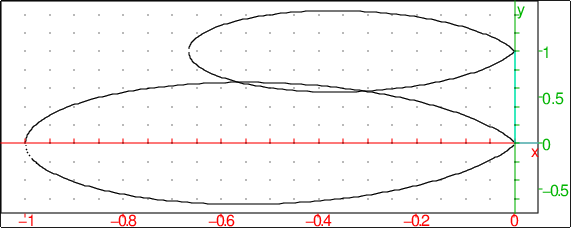
\includegraphics[width=0.75\textwidth]{catenoid_intersections.png}
\end{center}
We observe that there are exactly two catenaries satisfying the Euler-Lagrange necessary conditions and the given boundary conditions : the first with $K_0\approx -0.5$ and $c_1\approx 0.6$ resp.~the second with $K_0\approx -0.3$ and $c_1\approx 0.5$. We obtain the values of these constants more precisely by using {\tt fsolve}. Input :
\begin{center}
  \tt p1:=fsolve([eq1,eq2],p,[-0.5,0.6]);
  p2:=fsolve([eq1,eq2],p,[-0.3,0.5])
\end{center}
Output :
\begin{center}
  \tt [-0.56237423894,0.662588703113], [-0.30613431407,0.567138261119]
\end{center}
We check, for each catenary, whether the strong Legendre condition \[f_{y'\,y'}(x,y_k,y_k')>0\] holds for $k=1,2$. Input :
\begin{center}
  \tt y1:=subs(y0,p,p1):; y2:=subs(y0,p,p2):;
  D2f:=diff(f,diff(y(x),x),2):;
  solve([eval(subs(D2f,y=y1,y(x)=y1))<=0,x>=0,x<=1],x);
  solve([eval(subs(D2f,y=y2,y(x)=y2))<=0,x>=0,x<=1],x)
\end{center}
Output :
\begin{center}
  \tt [],[]
\end{center}
We conclude that the strong Legendre condition is satisfied in both cases, so we proceed by attempting to find the points conjugate to 0 for each catenary. The function $y_0$ depends on two parameters, so we use {\tt conjugate\_equation} to find these points easily. Input :
\begin{center}
  \tt fsolve(conjugate\_equation(y0,p,p1,x,0)=0,x=0..1)
  fsolve(conjugate\_equation(y0,p,p2,x,0)=0,x=0..1)
\end{center}
Output :
\begin{center}
  \tt [0.0], [0.0,0.799514772606]
\end{center}
We conclude that there are no points conjugate to $0$ in $(0,1]$ for the catenary $y_1$, so it minimizes the functional $F$. However, for the other catenary there is a conjugate point in the relevant interval, therefore $y_2$ is not a minimizer.

We can verify the above conclusions by computing the surface area for catenaries $y_1$ and $y_2$ and comparing them. Input :
\begin{center}
  \tt int(y1*sqrt(1+diff(y1,x)\verb|^|2),x=0..1); int(y2*sqrt(1+diff(y2,x)\verb|^|2),x=0..1)
\end{center}
Output :
\begin{center}
  \tt 0.81396915825,0.826468466845
\end{center}
We see that the surface formed by rotating the curve $y_1$ is indeed smaller than the area of the surface formed by rotating the curve $y_2$. Finally, we visualize both surfaces for convenience. Input :
\begin{center}
  \tt plot3d([y1*cos(t),y1*sin(t),x],x=0..1,t=0..2*pi, display=yellow+filled)
\end{center}
Output :
\begin{center}
  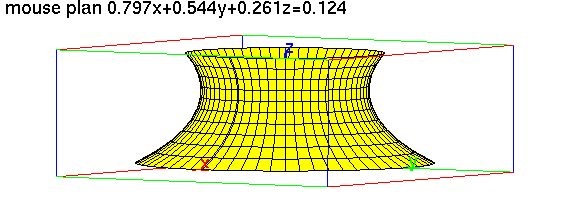
\includegraphics[width=0.75\textwidth]{catenoid_1.png}
\end{center}
Input :
\begin{center}
  \tt plot3d([y2*cos(t),y2*sin(t),x],x=0..1,t=0..2*pi, display=yellow+filled)
\end{center}
Output :
\begin{center}
  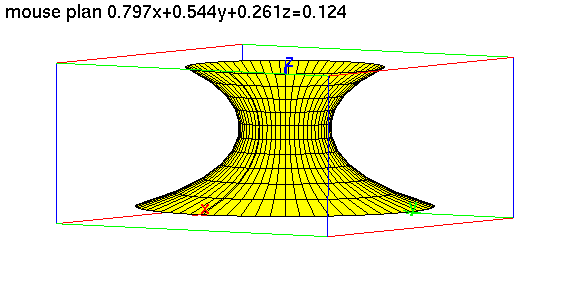
\includegraphics[width=0.75\textwidth]{catenoid_2.png}
\end{center}

\section{Limits}
\subsection{Limits : {\tt limit}}\index{limit|textbf}\label{sec:limit}

{\tt limit} computes the limit of an expression at a finite or infinite point.
It is also possible with an optional argument to  compute a one-sided
limit (1 for the right limit  and -1 for the left limit).\\
{\tt limit} takes three or four arguments :\\
an expression, the name of a variable (for example {\tt x}), the limit point 
(for example {\tt a}) and an optional argument, by default {\tt 0}, to 
indicate if the limit is unidirectional. 
This argument is equal to 
{\tt -1} for a left limit ({\tt x<a}) or  is equal to {\tt  1} 
for a right limit ({\tt x>a}) or is equal to {\tt 0} for a limit.\\
{\tt limit} returns the limit of the expression when the  variable (for example
{\tt x}) approaches the limit point (for example {\tt a}).\\
{\bf Remark}\\
It is also possible to put {\tt x=a} as  argument instead of {\tt x,a}, hence :
{\tt limit} takes also as arguments an expression depending of a variable, 
an equality (variable =value of the limit point) and perhaps 1 or -1 to 
indicate the direction.\\ 
Input :
\begin{center}{\tt limit(1/x,x,0,-1)}\end{center}
or :
\begin{center}{\tt limit(1/x,x=0,-1)}\end{center}
Output :
\begin{center}{\tt -(infinity)}\end{center} 
Input :
\begin{center}{\tt limit(1/x,x,0,1)}\end{center}
or :
\begin{center}{\tt limit(1/x,x=0,1)}\end{center}
Output :
\begin{center}{\tt +(infinity)}\end{center} 
Input :
\begin{center}{\tt limit(1/x,x,0,0)}\end{center}
or :
\begin{center}{\tt limit(1/x,x,0)}\end{center}
or :
\begin{center}{\tt limit(1/x,x=0)}\end{center}
Output :
\begin{center}{\tt infinity}\end{center} 
Hence, {\tt abs(1/x)} approaches $+\infty$ when $x$ approaches $0$.

{\bf Exercises} :
\begin{itemize}
\item Find for $n>2$, the limit  when $x$ approaches $0$ of :
$$ \frac{n\tan(x)-\tan(nx)}{\sin(nx)-n\sin(x)}$$
Input :
\begin{center}{\tt limit((n*tan(x)-tan(n*x))/(sin(n*x)-n*sin(x)),x=0)}\end{center}
Output :
\begin{center}{\tt 2 }\end{center}
\item Find the limit  when $x$ approaches $+\infty$ of :
$$\sqrt{x+\sqrt{x+\sqrt x}}-\sqrt x$$ 
Input :
\begin{center}{\tt limit(sqrt(x+sqrt(x+sqrt(x)))-sqrt(x),x=+infinity)}\end{center}
Output :
\begin{center}{\tt 1/2 }\end{center}
\item Find the limit  when $x$ approaches 0 of :
$$\frac{\sqrt{1+x+x^2/2}-\exp(x/2)}{(1-\cos(x))\sin(x)}$$ 
Input :
\begin{center}{\tt limit((sqrt(1+x+x\verb|^|2/2)-exp(x/2))/((1-cos(x))*sin(x)),x,0)}\end{center}
Output :
\begin{center}{\tt -1/6 }\end{center}
\end{itemize}

{\bf Remark}\\
To compute limits, it is better sometimes to quote the first argument.\\  
Input  :
\begin{center}{\tt limit('(2*x-1)*exp(1/(x-1))',x=+infinity)}\end{center}
Note that the first argument is quoted,  because it is better that
this argument is not simplified (i.e. not evaluated).\\
Output :
\begin{center}{\tt +(infinity)}\end{center}

\subsection{Integral and limit}\index{limit} \index{limit} 
Just two examples :\\
\begin{itemize}
\item Find the limit, when $a$ approaches $+\infty$, of :
$$  \int _2^a \frac {1}{x^2}\ dx$$
Input :
\begin{center}{\tt limit(integrate(1/(x\verb|^|2),x,2,a),a,+(infinity))}\end{center}
Output (if {\tt a} is assigned then input {\tt purge(a)}) :
\begin{center}{\tt 1/2}\end{center}
\item Find the limit, when $a$ approaches $+\infty$, of :
$$  \int _2^a (\frac {x}{x^2-1}+\ln(\frac {x+1}{x-1}))\ dx$$
Input :
\begin{center}{\tt limit(integrate(x/(x\verb|^|2-1)+log((x+1)/(x-1)),x,2,a),}\end{center} 
\begin{center}{\tt a,+(infinity))}\end{center} 
Output (if {\tt a} is assigned then input {\tt purge(a)}) :
\begin{center}{\tt +(infinity)}\end{center}
\end{itemize}

\section{Rewriting transcendental and trigonometric expressions}
\subsection{Expand a transcendental and trigonometric expression : {\tt texpand tExpand}}\index{texpand|textbf}\index{tExpand|textbf}
\noindent{\tt texpand} or {\tt tExpand} takes as argument an
expression containing transcendental or trigonometric functions.\\
{\tt texpand} or {\tt tExpand} expands these functions, like simultaneous
calling {\tt expexpand}, {\tt lnexpand} and {\tt trigexpand}, 
for example,  $\ln(x^n)$ becomes $\ n\ln(x)$, $\exp(nx)$ 
becomes $\ \exp(x)^n$, $\sin(2x)$ becomes $\ 2\sin(x)\cos(x)$...\\
{\bf Examples} :\\
\begin{itemize}
\item
\begin{enumerate}
\item Expand $\cos(x+y)$.\\
Input :
\begin{center}{\tt texpand(cos(x+y))}\end{center}
Output :
\begin{center}{\tt cos(x)*cos(y)-sin(x)*sin(y)}\end{center}
\item Expand $\cos(3x)$.\\
Input :
\begin{center}{\tt texpand(cos(3*x))}\end{center}
Output :
\begin{center}{\tt 4*(cos(x))\verb|^| 3-3*cos(x)}\end{center}
\item Expand $\displaystyle \frac{\sin(3*x)+\sin(7*x)}{\sin(5*x)}$.\\
Input :
\begin{center}{\tt texpand((sin(3*x)+sin(7*x))/sin(5*x))}\end{center}
Output
\begin{center}{\tt (4*(cos(x))\verb|^|2-1)*(sin(x)/(16*(cos(x))\verb|^|4- 12*(cos(x))\verb|^|2+1))/sin(x)+(64*(cos(x))\verb|^|6- 80*(cos(x))\verb|^|4+24*(cos(x))\verb|^|2-1)*sin(x)/ (16*(cos(x))\verb|^|4-12*(cos(x))\verb|^|2+1)/sin(x)}\end{center}
Output, after a simplification with {\tt normal(ans())} :
\begin{center}{\tt 4*(cos(x))\verb|^|2-2}\end{center}
\end{enumerate}
\item \begin{enumerate}
\item Expand $\exp(x+y)$.\\
Input :
\begin{center}{\tt texpand(exp(x+y))}\end{center}
Output :
\begin{center}{\tt exp(x)*exp(y)}\end{center}
\item Expand $\ln(x\times y)$.\\
Input :
\begin{center}{\tt texpand(log(x*y))}\end{center}
Output :
\begin{center}{\tt log(x)+log(y)}\end{center}
\item Expand $\ln(x^n)$.\\
Input :
\begin{center}{\tt  texpand(ln(x\verb|^|n))}\end{center}
Output :
\begin{center}{\tt n*ln(x)}\end{center}
\item Expand $\ln((e^2)+\exp(2*\ln(2))+\exp(\ln(3)+\ln(2)))$.\\
Input :
\begin{center}{\tt texpand(log(e\verb|^|2)+exp(2*log(2))+exp(log(3)+log(2)))}\end{center}
Output :
\begin{center}{\tt 6+3*2}\end{center}
Or input :
\begin{center}{\tt texpand(log(e\verb|^|2)+exp(2*log(2)))+ lncollect(exp(log(3)+log(2)))}\end{center}
Output :
\begin{center}{\tt 12}\end{center}
\end{enumerate}
\item 
Expand $\exp(x+y)+\cos(x+y)+\ln(3x^2)$.\\
Input :
\begin{center}{\tt texpand(exp(x+y)+cos(x+y)+ln(3*x\verb|^|2))}\end{center}
Output :
\begin{center}{\tt cos(x)*cos(y)-sin(x)*sin(y)+exp(x)*exp(y)+ ln(3)+2*ln(x)}\end{center}
\end{itemize}

\subsection{Combine terms of the same type  : {\tt combine}}\index{combine}\index{exp@{\sl exp}|textbf}\index{log@{\sl log}|textbf}\index{ln@{\sl ln}|textbf}\index{sin@{\sl sin}|textbf}\index{cos@{\sl cos}|textbf}\index{trig@{\sl trig}|textbf}
\noindent{\tt combine} takes two arguments : an expression and 
the name of a function or class of functions
{\tt exp,log,ln, sin,cos,trig}.\\
Whenever possible, {\tt combine} put together subexpressions corresponding
to the second argument:
\begin{itemize}
\item {\tt combine(expr,ln)} or {\tt combine(expr,log)} gives the same result 
as {\tt lncollect(expr)}
\item
{\tt combine(expr,trig)} or {\tt combine(expr,sin)}  or {\tt combine(expr,cos)}
gives the same result as {\tt tcollect(expr)}.
\end{itemize}
Input :
\begin{center}{\tt combine(exp(x)*exp(y)+sin(x)*cos(x)+ln(x)+ln(y),exp)}\end{center}
Output :
\begin{center}{\tt exp(x+y)+sin(x)*cos(x)+ln(x)+ln(y)}\end{center}
Input :
\begin{center}{\tt combine(exp(x)*exp(y)+sin(x)*cos(x)+ln(x)+ln(y),trig)}\end{center}
or
\begin{center}{\tt combine(exp(x)*exp(y)+sin(x)*cos(x)+ln(x)+ln(y),sin)}\end{center}
or
\begin{center}{\tt combine(exp(x)*exp(y)+sin(x)*cos(x)+ln(x)+ln(y),cos)}\end{center}
Output :
\begin{center}{\tt exp(y)*exp(x)+(sin(2*x))/2+ln(x)+ln(y)}\end{center}
Input :
\begin{center}{\tt combine(exp(x)*exp(y)+sin(x)*cos(x)+ln(x)+ln(y),ln)}\end{center}
or
\begin{center}{\tt combine(exp(x)*exp(y)+sin(x)*cos(x)+ln(x)+ln(y),log)}\end{center}
Output :
\begin{center}{\tt exp(x)*exp(y)+sin(x)*cos(x)+ln(x*y)}\end{center}

\section{Trigonometry}
\subsection{Trigonometric functions}\label{sec:trigo}
\begin{itemize}
\item {\tt sin} \index{sin} is the sine function,
\item {\tt cos} \index{cos}  is the cosine function,
\item  {\tt tan} \index{tan} is the tangent function ({\tt tan(x)=
    sin(x)/cos(x)}),
\item 
{\tt cot} \index{cot|textbf}  is the cotangent function ({\tt cot(x)=
  cos(x)/sin(x)}),
\item 
{\tt sec} \index{sec|textbf}  is the secant function ({\tt sec(x)=
  1/cos(x)}),
\item
{\tt csc} \index{csc|textbf}  is the cosecant function ({\tt csc(x) =
  1/sin(x)}),
\item
{\tt asin} or {\tt arcsin}\index{asin}\index{arcsin}, {\tt acos} or {\tt arccos}\index{acos}\index{arccos}, {\tt atan} or {\tt arctan}\index{atan}\index{arctan}, {\tt acot}\index{acot|textbf}, {\tt asec}\index{asec|textbf}, {\tt acsc}\index{acsc|textbf}
are the inverse trigonometric functions. The latter are defined by:
\begin{enumerate}
\item {\tt asec(x) = acos(1/x)}, 
\item
{\tt acsc(x) = asin(1/x)},
\item
{\tt  acot(x) = atan(1/x)}. 
\end{enumerate}
\end{itemize}


\subsection{Expand a trigonometric expression : {\tt trigexpand}}\index{trigexpand}
\noindent{\tt trigexpand} takes as argument an expression
containing trigonometric functions.\\
{\tt trigexpand} expands sums, differences and products by an integer
inside the trigonometric functions \\
Input :
\begin{center}{\tt trigexpand(cos(x+y))}\end{center}
Output :
\begin{center}{\tt cos(x)*cos(y)-sin(x)*sin(y)}\end{center}


\subsection{Linearize  a trigonometric expression : {\tt tlin}}\index{tlin}
\noindent{\tt tlin} takes as argument an expression
containing trigonometric functions.\\
{\tt tlin} linearizes products and integer powers of the trigonometric
functions (e.g. in terms of $\sin(n*x)$ and  
$\cos(n*x)$)\\
{\bf Examples}
\begin{itemize}
\item Linearize $\cos(x)*\cos(y)$.\\
Input :
\begin{center}{\tt tlin(cos(x)*cos(y))}\end{center}
Output :
\begin{center}{\tt 1/2*cos(x-y)+1/2*cos(x+y)}\end{center}
\item Linearize $\cos(x)^3$.\\
Input :
\begin{center}{\tt tlin(cos(x)\verb|^|3)}\end{center}
Output :
\begin{center}{\tt 3/4*cos(x)+1/4*cos(3*x)}\end{center}
\item Linearize $4\cos(x)^2-2$.\\
Input :
\begin{center}{\tt tlin(4*cos(x)\verb|^|2-2)}\end{center}
Output :
\begin{center}{\tt 2*cos(2*x)}\end{center}
\end{itemize}

\subsection{Increase the phase by $\pi/2$ in a trigonometric
expression: \texttt{shift\_phase}}\index{shift\_phase}

The \texttt{shift\_phase} command takes as argument a trigonometric
expression.\\
\texttt{shift\_phase} returns the expression with phase increased by
$\pi/2$ (after the automatic simplification).\\
Input:
\begin{center}
  \tt
  shift\_phase(x + sin(x))
\end{center}
Output:
\begin{center}
  \tt
 x-cos((pi+2*x)/2) 
\end{center}
Input:
\begin{center}
  \tt
  shift\_phase(x + cos(x))
\end{center}
Output:
\begin{center}
  \tt
  x+sin((pi+2*x)/2)
\end{center}
Input:
\begin{center}
  \tt
  shift\_phase(x + tan(x))
\end{center}
Output:
\begin{center}
  \tt
 x-1/tan((pi+2*x)/2) 
\end{center}

Quoting the argument will prevent the automatic simplification.\\
Input:
\begin{center}
  \tt
  shift\_phase('sin(x + pi/2)')
\end{center}
Output:
\begin{center}
  \tt
 -cos((pi+2*x+2*pi/2)/2) 
\end{center}
With an unquoted sine, we get:\\
Input
\begin{center}
  \tt
  shift\_phase(sin(x + pi/2))  
\end{center}
Output:
\begin{center}
  \tt
 sin((pi+2*x)/2) 
\end{center}
since \texttt{sin(x+pi/2)} is evaluated (in this case simplified)
before \texttt{shift\_phase} is called, and
\texttt{shift\_phase(cos(x))} returns \texttt{sin((pi+2*x)/2)}


\subsection{Put together sine and cosine of the same angle : {\tt tcollect tCollect}}\index{tcollect}\index{tCollect}
\noindent{\tt tcollect} or {\tt tCollect} takes as argument 
an expression containing trigonometric functions.\\
{\tt tcollect} first linearizes this expression 
(e.g. in terms of $\sin(n*x)$ and $\cos(n*x)$),  
then, puts together sine and cosine of the same angle.\\
Input :
\begin{center}{\tt tcollect(sin(x)+cos(x))}\end{center}
Output :
\begin{center}{\tt sqrt(2)*cos(x-pi/4)}\end{center}
Input :
\begin{center}{\tt tcollect(2*sin(x)*cos(x)+cos(2*x))}\end{center}
Output :
\begin{center}{\tt sqrt(2)*cos(2*x-pi/4)}\end{center}

\subsection{Simplify : {\tt simplify}}\index{simplify}
\noindent{\tt simplify} simplifies the expression.\\
As with all automatic simplifications, do not expect miracles,
you will have to use specific rewriting rules if it does not work.\\ 
Input :
\begin{center}{\tt simplify((sin(3*x)+sin(7*x))/sin(5*x))}\end{center}
Output :
\begin{center}{\tt 4*(cos(x))\verb|^|2-2}\end{center}
{\bf Warning} {\tt simplify} is more efficient in {\tt radian} mode (check 
{\tt radian} in the {\tt cas} configuration 
  or  input {\tt angle\_radian:=1}).


\subsection{Simplify trigonometric expressions : {\tt trigsimplify}}\index{trigsimplify}
\noindent{\tt trigsimplify} simplifies trigonometric expressions
by combining {\tt simplify}, {\tt texpand}, {\tt tlin}, {\tt tcollect}, {\tt trigsin}, {\tt trigcos} and {\tt trigtan} commands in a certain order.\\
Input :
\begin{center}{\tt trigsimplify((sin(x+y)-sin(x-y))/(cos(x+y)+cos(x-y)))}\end{center}
Output :
\begin{center}{\tt tan(y)}\end{center}
Input :
\begin{center}{\tt trigsimplify(1-1/4*sin(2a)\verb|^|2-sin(b)\verb|^|2-cos(a)\verb|^|4)}\end{center}
Output :
\begin{center}{\tt sin(a)\verb|^|2-sin(b)\verb|^|2}\end{center}

\subsection{Transform arccos into arcsin : {\tt acos2asin}}\index{acos2asin}
\noindent{\tt acos2asin} takes as argument an expression containing 
inverse trigonometric functions.\\
{\tt acos2asin}  replaces $\arccos(x)$ by 
$\displaystyle \frac{\pi}{2}-\arcsin(x)$ in this expression.\\
Input :
\begin{center}{\tt acos2asin(acos(x)+asin(x))}\end{center}
Output after simplification :
\begin{center}{\tt pi/2}\end{center}

\subsection{Transform arccos into arctan : {\tt acos2atan}}\index{acos2atan}
\noindent{\tt acos2atan} takes as argument an expression containing 
inverse trigonometric functions.\\
{\tt acos2atan}  replaces $\arccos(x)$ by
$\displaystyle \frac{\pi}{2}-\arctan(\frac{x}{\sqrt{1-x^2}})$ in this 
expression.\\
Input :
\begin{center}{\tt acos2atan(acos(x))}\end{center}
Output :
\begin{center}{\tt  pi/2-atan(x/sqrt(1-x\verb|^|2))}\end{center}

\subsection{Transform arcsin into arccos : {\tt asin2acos}}\index{asin2acos}
\noindent{\tt asin2acos} takes as argument an 
expression containing inverse trigonometric functions.\\
{\tt asin2acos} replaces $\arcsin(x)$  by
$\displaystyle \frac{\pi}{2}-\arccos(x)$ in this expression.\\
Input :
\begin{center}{\tt asin2acos(acos(x)+asin(x))}\end{center}
Output after simplification :
\begin{center}{\tt pi/2}\end{center}

\subsection{Transform arcsin into arctan : {\tt asin2atan}}\index{asin2atan}
\noindent{\tt asin2atan} takes as argument an expression containing 
inverse trigonometric functions.\\
{\tt asin2atan} replaces $\arcsin(x)$  by 
$\displaystyle \arctan(\frac{x}{\sqrt{1-x2}})$ in this expression.\\
Input :
\begin{center}{\tt asin2atan(asin(x))}\end{center}
Output :
\begin{center}{\tt atan(x/sqrt(1-x\verb|^|2))}\end{center}

\subsection{Transform arctan into arcsin : {\tt atan2asin}}\index{atan2asin}
\noindent{\tt atan2asin} takes as argument an expression
containing inverse trigonometric functions.
{\tt atan2asin} replaces $\arctan(x)$ by 
$\displaystyle \arcsin(\frac{x}{\sqrt{1+x2}})$ in this expression.\\
Input :
\begin{center}{\tt atan2asin(atan(x))}\end{center}
Output :
\begin{center}{\tt asin(x/sqrt(1+x\verb|^|2))}\end{center}

\subsection{Transform arctan into arccos : {\tt atan2acos}}\index{atan2acos}
\noindent{\tt atan2acos} takes as argument an expression containing 
inverse trigonometric functions.\\
{\tt atan2acos} replaces $\arctan(x)$ by 
$\displaystyle \frac{\pi}{2}-\arccos(\frac{x}{\sqrt{1+x2}})$ 
in this expression.\\
Input :
\begin{center}{\tt atan2acos(atan(x))}\end{center}
Output :
\begin{center}{\tt pi/2-acos(x/sqrt(1+x\verb|^|2))}\end{center}

\subsection{Transform complex exponentials into sin and cos : {\tt sincos exp2trig}}\index{sincos}\index{exp2trig}
\noindent{\tt sincos}  or {\tt exp2trig} takes as argument an expression 
containing complex exponentials.\\
{\tt sincos} or {\tt exp2trig} rewrites this expression in terms of  
$\sin$ and  $\cos$.\\
Input :
\begin{center}{\tt sincos(exp(i*x))}\end{center}
Output :
\begin{center}{\tt cos(x)+(i)*sin(x)}\end{center}
Input :
\begin{center}{\tt exp2trig(exp(-i*x))}\end{center}
Output :
\begin{center}{\tt cos(x)+(i)*(-(sin(x)))}\end{center}
Input :
\begin{center}{\tt simplify(sincos(((i)*(exp((i)*x))\verb|^|2-i)/(2*exp((i)*x))))}\end{center}
or :
\begin{center}{\tt simplify(exp2trig(((i)*(exp((i)*x))\verb|^|2-i)/(2*exp((i)*x))))}\end{center}
Output :
\begin{center}{\tt -sin(x)}\end{center}

\subsection{Transform tan(x) into sin(x)/cos(x) : {\tt tan2sincos}}\index{tan2sincos}
\noindent{\tt tan2sincos} takes as argument an expression containing 
trigonometric functions.\\
{\tt tan2sincos} replaces $\tan(x)$ by
 $\displaystyle \frac{\sin(x)}{\cos(x)}$ in this expression.\\
Input :
\begin{center}{\tt tan2sincos(tan(2*x))}\end{center}
Output :
\begin{center}{\tt sin(2*x)/cos(2*x)}\end{center}

\subsection{Transform sin(x) into cos(x)*tan(x):
\texttt{sin2costan}}\index{sin2costan}

The \texttt{sin2costan} command takes as argument a trigonometric
expression.\\
\texttt{sin2costan} returns the expression with $\sin(x)$ replaced by
$\cos(x)\tan(x)$.\\
Input:
\begin{center}
  \tt
  sin2costan(sin(2*x))
\end{center}
Output:
\begin{center}
  \tt
 tan(2*x)*cos(2*x) 
\end{center}

\subsection{Transform cos(x) into sin(x)/tan(x):
\texttt{cos2sintan}}\index{cos2sintan}

The \texttt{cos2sintan} command takes as argument a trigonometric
expression.\\
\texttt{cos2sintan} returns the expression with $\cos(x)$ replaced by
$\sin(x)/\tan(x)$.\\
Input:
\begin{center}
  \tt
  cos2sintan(cos(2*x))
\end{center}
Output:
\begin{center}
  \tt
 sin(2*x)/tan(2*x)
\end{center}

\subsection{Rewrite tan(x) with sin(2x) and  cos(2x) : {\tt tan2sincos2}}\index{tan2sincos2}
\noindent{\tt tan2sincos2} takes as argument an expression containing 
trigonometric functions.\\
{\tt tan2sincos2} replaces $\tan(x)$ by 
$\displaystyle \frac{\sin(2x)}{1+\cos(2x)}$ in this  expression.\\
Input :
\begin{center}{\tt tan2sincos2(tan(x))}\end{center}
Output :
\begin{center}{\tt sin(2*x)/(1+cos(2*x))}\end{center}

\subsection{Rewrite tan(x) with cos(2x) and  sin(2x) : {\tt tan2cossin2}}\index{tan2cossin2}
\noindent{\tt tan2cossin2} takes as argument an expression 
containing trigonometric functions.\\
{\tt tan2cossin2} replaces $\tan(x)$ by 
$\displaystyle \frac{1-\cos(2x)}{\sin(2x)}$ , in this expression.\\
Input :
\begin{center}{\tt tan2cossin2(tan(x))}\end{center}
Output :
\begin{center}{\tt (1-cos(2*x))/sin(2*x)}\end{center}

\subsection{Rewrite sin, cos, tan in terms of tan(x/2) : {\tt halftan}}\index{halftan}
\noindent{\tt halftan} takes as argument an expression 
containing trigonometric functions.\\
{\tt halftan} rewrites $\sin(x),\ \cos(x)$ and  $ \tan(x)$ 
 in terms of $\tan(\frac{x}{2})$.\\
Input :
\begin{center}{\tt halftan(sin(2*x)/(1+cos(2*x)))}\end{center}
Output :
\begin{center}{\tt 2*tan(2*x/2)/((tan(2*x/2))\verb|^|2+1)/}\end{center}
\begin{center}{\tt (1+(1-(tan(2*x/2))\verb|^|2)/((tan(2*x/2))\verb|^|2+1))}\end{center}
Output, after simplification with {\tt normal(ans())} :
\begin{center}{\tt tan(x)}\end{center}
Input :
\begin{center}{\tt halftan(sin(x)\verb|^|2+cos(x)\verb|^|2)}\end{center}
Output :
\begin{center}{\tt (2*tan(x/2)/((tan(x/2))\verb|^|2+1))\verb|^|2+}\end{center}
\begin{center}{\tt ((1-(tan(x/2))\verb|^|2)/((tan(x/2))\verb|^|2+1))\verb|^|2}\end{center}
Output, after simplification with {\tt normal(ans())} :
\begin{center}{\tt 1}\end{center}

\subsection{Rewrite trigonometric functions as function of tan(x/2) 
and hyperbolic functions as function of exp(x):
{\tt halftan\_hyp2exp}}\index{halftan\_hyp2exp}
\noindent{\tt halftan\_hyp2exp} takes as argument a trigonometric and  
hyperbolic expression.\\
{\tt halftan\_hyp2exp} rewrites $\sin(x),\ \cos(x), \tan(x)$ 
 in terms of $\tan(\frac{x}{2})$ 
and $\sinh(x),\ \cosh(x), \tanh(x)$ in terms of $\exp(x)$.\\
Input :
\begin{center}{\tt halftan\_hyp2exp(tan(x)+tanh(x))}\end{center}
Output :
\begin{center}{\tt (2*tan(x/2))/((1-(tan(x/2))\verb|^|2))+(((exp(x))\verb|^|2-1))/ (((exp(x))\verb|^|2+1))}\end{center}
Input :
\begin{center}{\tt halftan\_hyp2exp(sin(x)\verb|^|2+cos(x)\verb|^|2-sinh(x)\verb|^|2+cosh(x)\verb|^|2)}\end{center}
Output, after simplification with {\tt normal(ans())} :
\begin{center}{\tt 2}\end{center}

\subsection{Transform inverse trigonometric functions into logarithms : {\tt atrig2ln}}\index{atrig2ln}
\noindent{\tt atrig2ln}  takes as argument an expression containing
inverse trigonometric functions.\\
{\tt atrig2ln} rewrites these functions with complex logarithms.\\
Input :
\begin{center}{\tt atrig2ln(asin(x))}\end{center}
Output :
\begin{center}{\tt i*log(x+sqrt(x\verb|^|2-1))+pi/2}\end{center}

\subsection{Transform trigonometric functions into complex exponentials  : {\tt trig2exp}}\index{trig2exp}
\noindent{\tt trig2exp} takes as argument an expression containing 
trigonometric functions.\\
{\tt trig2exp} rewrites the trigonometric functions with complex exponentials
({\sc without} linearization).\\ 
Input :
\begin{center}{\tt trig2exp(tan(x))}\end{center}
Output :
\begin{center}{\tt ((exp((i)*x))\verb|^|2-1)/((i)*((exp((i)*x))\verb|^|2+1))}\end{center}
Input :
\begin{center}{\tt trig2exp(sin(x))}\end{center}
Output :
\begin{center}{\tt (exp((i)*x)-1/(exp((i)*x)))/(2*i)}\end{center}

\subsection{Simplify and express preferentially with sine : {\tt trigsin}}\index{trigsin}
\noindent{\tt trigsin} takes as argument an expression
containing trigonometric functions.\\
{\tt trigsin} simplify this expression with the formula :\\
$\sin(x)^2+\cos(x)^2=1$, $\displaystyle \tan(x)=\frac{\sin(x)}{\cos(x)}$ and 
tries to rewrite the expression only with sine.\\ 
Input :
\begin{center}{\tt trigsin(sin(x)\verb|^|4+cos(x)\verb|^|2+1)}\end{center}
Output :
\begin{center}{\tt sin(x)\verb|^|4-sin(x)\verb|^|2+2}\end{center}

\subsection{Simplify and express preferentially with cosine : {\tt trigcos}}\index{trigcos}
\noindent{\tt trigcos} takes as argument an expression
containing trigonometric functions.\\
{\tt trigcos} simplifies this expression with the formula :\\
$\sin(x)^2+\cos(x)^2=1$, $\displaystyle \tan(x)=\frac{\sin(x)}{\cos(x)}$  and  
tries to rewrite the expression only with cosine.\\ 
Input :
\begin{center}{\tt trigcos(sin(x)\verb|^|4+cos(x)\verb|^|2+1)}\end{center}
Output :
\begin{center}{\tt cos(x)\verb|^|4-cos(x)\verb|^|2+2}\end{center}

\subsection{Simplify and express preferentially with tangents : {\tt trigtan}}\index{trigtan}
\noindent{\tt trigtan} takes as argument an expression 
containing trigonometric functions.\\
{\tt trigtan} simplifies this expression with the formula :\\
$\sin(x)^2+\cos(x)^2=1$, $\displaystyle \tan(x)=\frac{\sin(x)}{\cos(x)}$ and  
tries to rewrite the expression only with tangents.\\ 
Input :
\begin{center}{\tt trigtan(sin(x)\verb|^|4+cos(x)\verb|^|2+1)}\end{center}
Output :
\begin{center}{\tt((tan(x))\verb|^|2/(1+(tan(x))\verb|^|2))\verb|^|2+1/(1+(tan(x)\verb|^|2)+1}\end{center}
Output, after simplification with {\tt normal} :
\begin{center}{\tt (2*tan(x)\verb|^|4+3*tan(x)\verb|^|2+2)/(tan(x)\verb|^|4+2*tan(x))\verb|^|2+1)}\end{center}

\subsection{Rewrite an expression with different options : 
{\tt convert convertir =>}}
\index{convert|textbf}\index{convertir|textbf}\index{=>}\index{sin@{\sl sin}|textbf}
\index{cos@{\sl cos}|textbf}\index{sincos@{\sl sincos}|textbf}
\index{exp@{\sl exp}|textbf}\index{tan@{\sl tan}|textbf}\index{ln@{\sl ln}|textbf}
\index{expln@{\sl expln}|textbf}\index{string@{\sl string}|textbf}
\index{matrix@{\sl matrix}|textbf}\index{polynom@{\sl polynom}}
\index{parfrac@{\sl parfrac}|textbf}\index{partfrac@{\sl partfrac}|textbf}
\index{fullparfrac@{\sl fullparfrac}|textbf}
\label{sec:convert}
\noindent{\tt convert} takes two arguments, an expression and an
option. \texttt{=>} is the infixed version of \texttt{convert}.\\
{\tt convert} rewrites this expression applying rules depending 
on the option. Valid options are :
\begin{itemize}
\item{\tt sin} converts an expression like {\tt trigsin}.
\item{\tt cos} converts an expression like {\tt trigcos}.
\item{\tt sincos} converts an expression like {\tt sincos}.
\item{\tt trig} converts an expression like {\tt sincos}.
\item{\tt tan} converts an expression like {\tt halftan}.
\item{\tt exp} converts an expression like {\tt trig2exp}.
\item{\tt ln} converts an expression like {\tt trig2exp}.
\item{\tt expln} converts an expression like {\tt trig2exp}.
\item{\tt string} converts an expression into a string.
\item{\tt matrix} converts a list of lists into a matrix.
\item{\tt polynom} converts a Taylor series into a polynomial 
by removing the remainder (cf \ref{sec:convertpoly}).
\item{\tt parfrac} or {\tt partfrac} or {\tt fullparfrac} converts a rational 
fraction into its partial fraction decomposition (\ref{sec:convertparf}).
\end{itemize}
{\tt convert} can also :
\begin{itemize}
\item convert units, for example 
{\tt convert(1000\_g,\_kg)=1.0\_kg} (cf \ref{sec:convertunit}).
\item write a real as a continued fraction  : 
{\tt convert(a,confrac,'fc')} writes {\tt a} as a continued fraction
stored in {\tt fc}. Do not forget to quote the last argument if it
was assigned.\\
For example, {\tt convert(1.2,confrac,'fc')=[1,5]} and  {\tt fc} contains the 
continued fraction equal to 1.2 (cf \ref{sec:convertdfc}). 
\item  transform an integer into the list of its digits in a 
base, beginning with the units digit (and reciprocally)
\begin{itemize}
\item
{\tt convert(n,base,b)} transforms the integer {\tt n} into the list of its 
digits in base {\tt b} beginning with the units digit.\\ For example,
{\tt convert(123,base,10)=[3,2,1]} and  reciprocally
\item
{\tt convert(l,base,b)} transforms the list {\tt l} into the integer {\tt n} 
which has {\tt l} as list of its 
digits in base {\tt b} beginning with the units digit.\\ For example, 
{\tt convert([3,2,1],base,10)=123} (cf \ref{sec:convertbase}). 
\end{itemize}
\end{itemize}

\section{Fourier transformation}
\subsection{Fourier coefficients : {\tt fourier\_an} and  {\tt fourier\_bn} or {\tt fourier\_cn}} \index{integer}
Let $f$ be a $T$-periodic continuous functions on
$\mathbb{R}$ except maybe at a finite number of points.
One can prove that if $f$ is continuous at $x$, then;
\begin{eqnarray*}
f(x)&=&\frac{a_0}{2}+\sum _{n=1}^{+\infty} a_n \cos(\frac{2\pi
  nx}{T})+b_n \sin(\frac{2\pi nx}{T}) \\
 &=&\sum _{n=-\infty}^{+\infty} c_n e^{\frac{2i\pi nx}{T}}
\end{eqnarray*}
where the coefficients $a_n,\ b_n$, $n\in N$, (or $c_n$, $n \in Z$) are the 
Fourier coefficients of $f$.
The commands{\tt fourier\_an} and {\tt fourier\_bn} or {\tt fourier\_cn} 
compute these coefficients.  

\subsubsection{\tt fourier\_an}\index{fourier\_an}\label{sec:fourier_an}
\noindent{\tt fourier\_an} takes four or five arguments : an expression $expr$
depending on a variable, the name of this variable (for example $x$), the 
period $T$, an integer $n$ and a real $a$ (by default $a=0$).\\
{\tt fourier\_an(expr,x,T,n,a)} returns the Fourier coefficient $a_n$ of a 
function $f$ of 
variable $x$ defined on $[a,a+T)$ by $f(x)=expr$ and such that
$f$ is periodic of period $T$:
$$\displaystyle a_n=\frac{2}{T}\int_a^{a+T}f(x)\cos(\frac{2\pi nx }{T})dx$$
To simplify the computations, one should input {\tt assume(n,integer)} 
before calling {\tt fourier\_an} to specify 
that $n$ is an integer.\\
{\bf Example} Let the function $f$, of period $T=2$, defined on $[-1,1)$ by 
$f(x)=x^2$.\\
Input, to have the coefficient $a_0$ :
\begin{center}{\tt fourier\_an(x\verb|^|2,x,2,0,-1)}\end{center}
Output :
\begin{center}{\tt 1/3}\end{center}
Input, to have the coefficient $a_n$ ($n\neq 0$) :
 \begin{center}{\tt assume(n,integer);fourier\_an(x\verb|^|2,x,2,n,-1)}\end{center}
Output :
\begin{center}{\tt 4*(-1)\verb|^|n/(pi\verb|^|2*n\verb|^|2)}\end{center}

\subsubsection{\tt fourier\_bn}\index{fourier\_bn}\label{sec:fourier_bn}
\noindent{\tt fourier\_bn} takes four or five arguments : an expression $expr$
depending on a variable, the name of this variable (for example $x$), the 
period $T$, an integer $n$ and a real $a$ (by default $a=0$).\\
{\tt fourier\_bn(expr,x,T,n,a)} returns the Fourier coefficient $b_n$ of a 
function $f$ of variable $x$ defined on $[a,a+T)$ by $f(x)=expr$ and  periodic 
of period $T$:
$$\displaystyle b_n=\frac{2}{T}\int_a^{a+T}f(x)\sin(\frac{2\pi nx}{T})dx$$
To simplify the computations, one should input {\tt assume(n,integer)} 
before calling {\tt fourier\_bn} to specify that $n$ is an integer.\\
{\bf Examples} 
\begin{itemize}
\item Let the function $f$, of period $T=2$, defined on $[-1,1)$ by 
$f(x)=x^2$.\\
Input, to have the coefficient $b_n$ ($n\neq 0$) :
 \begin{center}{\tt  assume(n,integer);fourier\_bn(x\verb|^|2,x,2,n,-1)}\end{center}
Output :
\begin{center}{\tt  0}\end{center}

\item Let the function $f$, of period $T=2$, defined on $[-1,1)$ by
$f(x)=x^3$.\\
Input, to have the coefficient  $b_1$ :
 \begin{center}{\tt fourier\_bn(x\verb|^|3,x,2,1,-1)}\end{center}
Output :
\begin{center}{\tt (2*pi\verb|^|2-12)/pi\verb|^|3}\end{center}
\end{itemize}

\subsubsection{\tt fourier\_cn}\index{fourier\_cn}\label{sec:fourier_cn}
\noindent{\tt fourier\_cn} takes four or five arguments : an expression $expr$
depending of a variable, the name of this variable (for example $x$), the 
period $T$, an integer $n$ and a real $a$ (by default $a=0$).\\
{\tt fourier\_cn(expr,x,T,n,a)} returns the Fourier coefficient $c_n$ of a 
function$f$ of variable $x$ defined on $[a,a+T)$ by $f(x)=expr$ and  periodic 
of period $T$:
$$\displaystyle c_n=\frac{1}{T}\int_a^{a+T}f(x)e^{\frac{-2i\pi nx}{T}}dx$$
To simplify the computations, one should
input {\tt assume(n,integer)} before calling {\tt fourier\_cn}
to specify that $n$ is an integer.\\
{\bf Examples}
\begin{itemize}
\item Find the Fourier coefficients $c_n$ of the periodic function $f$ of
period $2$ and  defined on $[-1,1)$ by $ f(x)=x^2$.\\ 
Input, to have $c_0$ :
\begin{center}{\tt fourier\_cn(x\verb|^|2,x,2,0,-1)}\end{center}
Output:
\begin{center}{\tt 1/3}\end{center}
Input, to have $c_n$ :
\begin{center}{\tt assume(n,integer)}\end{center}
\begin{center}{\tt fourier\_cn(x\verb|^|2,x,2,n,-1)}\end{center}
Output:
\begin{center}{\tt 2*(-1)\verb|^|n/(pi\verb|^|2*n\verb|^|2)}\end{center}

\item Find the Fourier coefficients $c_n$ of the periodic function $f$, of 
period $2$, and defined on $[0,2)$ by $ f(x)=x^2$.\\ 
Input,  to have $c_0$ :
\begin{center}{\tt fourier\_cn(x\verb|^|2,x,2,0)}\end{center}
Output:
\begin{center}{\tt 4/3}\end{center}
Input, to have $c_n$ :
\begin{center}{\tt assume(n,integer)}\end{center}
\begin{center}{\tt fourier\_cn(x\verb|^|2,x,2,n)}\end{center}
Output:
\begin{center}{\tt ((2*i)*pi*n+2)/(pi\verb|^|2*n\verb|^|2)}\end{center}

\item Find the Fourier coefficients $c_n$ of the periodic function $f$ of 
period $2\pi$ and  defined on $[0,2\pi)$ by $ f(x)=x^2$.\\ 
Input \index{assume} :
\begin{center}{\tt assume(n,integer)}\end{center}
\begin{center}{\tt fourier\_cn(x\verb|^|2,x,2*pi,n)}\end{center}
Output :
\begin{center}{\tt ((2*i)*pi*n+2)/n\verb|^|2}\end{center}
If you don't specify {\tt assume(n,integer)}, the output will not be 
simplified :
\begin{center}{\tt ((2*i)*pi\verb|^|2*n\verb|^|2*exp((-i)*n*2*pi)+2*pi*n*exp((-i)*n*2*pi)+}\end{center}
\begin{center}{\tt (-i)*exp((-i)*n*2*pi)+i)/(pi*n\verb|^|3)}\end{center}
You might simplify this expression by replacing 
{\tt exp((-i)*n*2*pi)} by {\tt 1}, input :
\begin{center}{\tt subst(ans(),exp((-i)*n*2*pi)=1)}\end{center}
Output :
\begin{center}{\tt ((2*i)*pi\verb|^|2*n\verb|^|2+2*pi*n+-i+i)/pi/n\verb|^|3}\end{center}
This expression is then simplified with {\tt normal}, the final
output is :
\begin{center}{\tt ((2*i)*pi*n+2)/n\verb|^|2}\end{center}
Hence for $n \neq 0$, $\displaystyle c_n=\frac{2in\pi+2}{n^2}$.
As shown in this example, it is better to input  {\tt
  assume(n,integer)} before calling {\tt fourier\_cn}.\\
We must also compute $c_n$ for $n=0$, input :
\begin{center}{\tt fourier\_cn(x\verb|^|2,x,2*pi,0)}\end{center}
Output :
\begin{center}{\tt  4*pi\verb|^|2/3}\end{center}
Hence for  $n= 0$, $\displaystyle c_0=\frac{4{\pi}^2}{3}$. 
\end{itemize}
{\bf Remarks} :
\begin{itemize}
\item Input {\tt purge(n)}\index{purge} to remove the hypothesis done
  on $n$.
\item
Input {\tt about(n)}\index{about} or {\tt assume(n)}\index{assume}, to know 
the hypothesis done on the variable $n$.
\end{itemize}

\subsection{Continuous Fourier Transform : {\tt fourier}\index{fourier}, {\tt ifourier}\index{ifourier}}
The command {\tt fourier} takes one to three arguments: an expression $ f(x) $ and (optionally) identifiers $ x $ and $ s $. It returns the Fourier transform $ F $ of $ f $ defined by
\begin{equation}\label{eq:fourier-def}
F(s)=\int_{-\infty}^{+\infty}\mathrm{e}^{-\mathrm{i}\,s\,x}\,f(x)\,\mathrm{d}x,\quad s\in\mathbb{R}.
\end{equation}
If $ s $ is not given, $ F $ is returned as a function of $ x $.

The command {\tt ifourier} works the other way round: it takes arguments $ F(s) $ and (optionally) $ s $ and $ x $, and returns the expression $ f(x) $ using the formula
\[ f(x)=\frac{1}{2\,\pi}\,\int_{-\infty}^{+\infty}\mathrm{e}^{\mathrm{i}\,s\,x}\,F(s)\,\mathrm{d}s. \]
To compute the above integral, {\tt fourier} is called with input parameters $ \frac{F(s)}{2\,\pi} $, $ s $ and $ x $, replacing $ x $ with $ -x $ in the result.

Arbitrary rational functions can be transformed. For example, to find the Fourier transform of $ f(x)=\frac{x}{x^3-19\,x+30} $, input :
\begin{center}
  \tt F:=fourier(x/(x\^{}3-19x+30),x,s)
\end{center}
Output :
\begin{center}
  \tt pi*(5*i*exp(5*i*s)+(-21*i)*exp((-3*i)*s)+16*i*exp((-2*i)*s))*sign(s)/56
\end{center}
Input :
\begin{center}
  \tt ifourier(F,s,x)
\end{center}
Output :
\begin{center}
  \tt x/(x\^{}3-19*x+30)
\end{center}
Similarly, to find the transform of $ f(x)=\frac{x^2+1}{x^2-1} $, input :
\begin{center}
  \tt F:=fourier((x\^{}2+1)/(x\^{}2-1),x,s)
\end{center}
Output :
\begin{center}
  \tt 2*pi*(Dirac(s)-sign(s)*sin(s))
\end{center}
Input :
\begin{center}
  \tt ifourier(F,s,x)
\end{center}
Output :
\begin{center}
  \tt (x\^{}2+1)/(x\^{}2-1)
\end{center}
A range of other (generalized) functions and distributions can be transformed, as demonstrated in the following examples. If {\tt fourier} does not know how to transform a function, say $ f $, it returns the unevaluated integral~\eqref{eq:fourier-def}. In these cases one may try to evaluate the result using {\tt eval}.\\
Input :
\begin{center}
  \tt fourier(3x\^{}2+2x+1,x,s)
\end{center}
Output :
\begin{center}
  \tt 2*pi*(Dirac(s)+2*i*Dirac(s,1)-3*Dirac(s,2))
\end{center}
Input :
\begin{center}
  \tt fourier(Dirac(x-1)+Dirac(x+1),x,s)
\end{center}
Output :
\begin{center}
  \tt 2*cos(s)
\end{center}
Input :
\begin{center}
  \tt fourier(exp(-2*abs(x-1)),x,s)
\end{center}
Output :
\begin{center}
  \tt 4*exp(-i*s)/(s\^{}2+4)
\end{center}
Input :
\begin{center}
  \tt fourier(atan(1/(2x\^{}2)),x,s)
\end{center}
Output :
\begin{center}
  \tt 2*pi*sin(s/2)*exp(-abs(s)/2)/s
\end{center}
Input :
\begin{center}
  \tt fourier(BesselJ(3,x),x,s)
\end{center}
Output :
\begin{center}
  \tt -s*(4*s\^{}2-3)*(-i*sign(s+1)+i*sign(s-1))/sqrt(-s\^{}2+1)
\end{center}
Input :
\begin{center}
  \tt F:=fourier(sin(x)*sign(x),x,s)
\end{center}
Output :
\begin{center}
  \tt -2/(s\^{}2-1)
\end{center}
Input :
\begin{center}
  \tt ifourier(F,s,x)
\end{center}
Output :
\begin{center}
  \tt sign(x)*sin(x)
\end{center}
Input :
\begin{center}
  \tt fourier(log(abs(x)),x,s)
\end{center}
Output :
\begin{center}
  \tt -pi*(2*euler\_gamma*Dirac(s)*abs(s)+1)/abs(s)
\end{center}
Input :
\begin{center}
  \tt fourier(rect(x),x,s)
\end{center}
Output :
\begin{center}
  \tt 2*sin(s/2)/s
\end{center}
Input :
\begin{center}
  \tt fourier(exp(-abs(x))*sinc(x),x,s)
\end{center}
Output :
\begin{center}
  \tt atan(s+1)-atan(s-1)
\end{center}
Input :
\begin{center}
  \tt fourier(1/sqrt(abs(x)),x,s)
\end{center}
Output :
\begin{center}
  \tt sqrt(2)*sqrt(pi)/sqrt(abs(s))
\end{center}
Input :
\begin{center}
  \tt F:=fourier(1/cosh(2x),x,s)
\end{center}
Output :
\begin{center}
  \tt pi/(exp(pi*s/4)+exp(-pi*s/4))
\end{center}
Input :
\begin{center}
  \tt ifourier(F,s,x)
\end{center}
Output :
\begin{center}
  \tt 2/(exp(2*x)+exp(-2*x))
\end{center}
Input :
\begin{center}
  \tt fourier(Airy\_Ai(x/2),x,s)
\end{center}
Output :
\begin{center}
  \tt 2*exp(8*i*s\^{}3/3)
\end{center}
Input :
\begin{center}
  \tt F:=fourier(Gamma(1+i*x/3),x,s)
\end{center}
Output :
\begin{center}
  \tt 6*pi*exp(-exp(-3*s)-3*s)
\end{center}
Input :
\begin{center}
  \tt ifourier(F,s,x)
\end{center}
Output :
\begin{center}
  \tt Gamma(i*x/3+1)
\end{center}
Input :
\begin{center}
  \tt F:=fourier(atan(x/4)/x,x,s)
\end{center}
Output :
\begin{center}
  \tt pi*ugamma(0,4*abs(s))
\end{center}
Input :
\begin{center}
  \tt ifourier(F,s,x)
\end{center}
Output :
\begin{center}
  \tt atan(x/4)/x
\end{center}
Input :
\begin{center}
  \tt assume(a>0):; fourier(exp(-a*x\^{}2+b),x,s)
\end{center}
Output :
\begin{center}
  \tt sqrt(a)*sqrt(pi)*exp(-s\^{}2/(4*a)+b)/a
\end{center}
In the following example we compute the convolution of $ f(x)=\mathrm{e}^{-|x|} $ with itself using the convolution theorem. Input :
\begin{center}
  \tt F:=fourier(exp(-abs(x)),x,s)
\end{center}
Output :
\begin{center}
  \tt 2/(s\^{}2+1)
\end{center}
Input :
\begin{center}
  \tt ifourier(F\^{}2,s,x)
\end{center}
Output :
\begin{center}
  \tt x*Heaviside(x)*exp(-x)-x*Heaviside(-x)*exp(x)+exp(-abs(x))
\end{center}
The above result is the desired convolution $ f\ast f(x)=\int_{-\infty}^{+\infty}f(t)\,f(x-t)\,\mathrm{d}t $.

Piecewise functions can be transformed if defined as
\begin{center}
  \tt piecewise(x<a1,f1,x<a2,f2,...,x<an,fn,f0)
\end{center}
where $ a_1,a_2,\dots,a_n $ are real numbers such that $ a_1<a_2<\cdots<a_n $. Inequalities may be strict or non-strict.\\
Input :
\begin{center}
  \tt f:=piecewise(x<=-1,exp(x+1),x<=1,1,exp(2-2x)):; F:=fourier(f,x,s)
\end{center}
Output :
\begin{center}
  \tt (-i*s*sin(s)+3*s*cos(s)+4*sin(s))/(s*(s-2*i)*(s+i))
\end{center}
The original function $ f $ is obtained from the above result by applying {\tt ifourier}. Input :
\begin{center}
  \tt ifourier(F,s,x)
\end{center}
Output :
\begin{center}
  \tt Heaviside(x+1)-Heaviside(x-1)+Heaviside(x-1)*exp(-2*x+2)+ Heaviside(-x-1)*exp(x+1)
\end{center}
One may verify that the above expression is equal to $ f(x) $ by plotting.

To transform unknown functions, one can use the command {\tt addtable}\index{addtable} which takes five arguments: {\tt fourier} or {\tt laplace} (to indicate the desired transform definition), $ f(x) $, $ F(s) $, $ x $ and $ s $, where $ f $, $ F $, $ x $ and $ s $ are identifiers. If the first argument is {\tt fourier}, this means that $ \mathcal{F}\{f(x)\}(s)=F(s) $ i.e.~that the command
\begin{center}
  \tt fourier(f(x),x,s)
\end{center}
would return {\tt F(s)}. The return value of {\tt addtable} is 1 on success and 0 on failure. The second and the third argument can also be expressions depending on several variables.\\
Input :
\begin{center}
  \tt addtable(fourier,y(x),Y(s),x,s)
\end{center}
Output :
\begin{center}
  \tt 1
\end{center}
Input :
\begin{center}
  \tt fourier(y(a*x+b),x,s)
\end{center}
Output :
\begin{center}
  \tt Y(s/a)*exp(i*s*b/a)/abs(a)
\end{center}
Input :
\begin{center}
  \tt fourier(Y(x),x,s)
\end{center}
Output :
\begin{center}
  \tt 2*pi*y(-s)
\end{center}
Input :
\begin{center}
  \tt addtable(fourier,g(x,t),G(s,t),x,s)
\end{center}
Output :
\begin{center}
  \tt 1
\end{center}
Input :
\begin{center}
  \tt fourier(g(x/2,3*t),x,s)
\end{center}
Output :
\begin{center}
  \tt 2*G(2*s,3*t)
\end{center}

Fourier transform can be used for solving linear differential equations with constant coefficients. For example, we obtain a particular solution to the equation
\[ y(x)+4\,y^{(4)}(x)=\delta(x), \]
where $ \delta $ is the Dirac delta function. First we transform both sides of the above equation. Input :
\begin{center}
  \tt L:=fourier(y(x)+4*diff(y(x),x,4),x,s); R:=fourier(Dirac(x),x,s)
\end{center}
Output :
\begin{center}
  \tt Y(s)-4*s\^{}4*Y(s), 1
\end{center}
Then we solve the equation $ L=R $ for $ Y(s) $. Generally, one should apply {\tt csolve} instead of {\tt solve}. Input :
\begin{center}
  \tt sol:=csolve(L=R,Y(s))[0]
\end{center}
Output :
\begin{center}
  \tt 1/(4*s\^{}4+1)
\end{center}
Finally, we apply {\tt ifourier} to obtain $ y(x) $. Input :
\begin{center}
  \tt ifourier(sol,s,x)
\end{center}
Output :
\begin{center}
  \tt (sin(abs(x)/2)+cos(abs(x)/2))*exp(-abs(x)/2)/4
\end{center}
The above solution can be combined with solutions of the corresponding homogeneous equation to obtain the general solution.

\subsection{Discrete Fourier Transform}
Let $N$ be an integer.
The Discrete Fourier Transform (DFT) is a transformation $F_N$ defined on
the set of periodic sequences of period $N$, it depends on a choice
of a primitive $N$-th root of unity $\omega_N$. If the
DFT is defined on sequences with complex coefficients, we take:
\[ \omega_N=e^{\frac{2 i \pi}{N}}\]
If $x$ is a periodic sequence of period 
$N$, defined by the vector $x=[x_0,x_1,...x_{N-1}]$ then 
$F_N(x)=y$ is a periodic sequence of period $N$, defined by:
\[ {(F_{N,\omega_N}(x))}_k=y_k=\sum_{j=0}^{N-1}x_j\omega_N^{-k\cdot j}, k=0..N-1 \]
where $\omega_N$ is a primitive $N$-th root of unity. 
The discrete Fourier transform may be computed faster than by
computing each $y_k$ individually, by the Fast Fourier Transform (FFT).
{\tt Xcas} implements the FFT algorithm to compute
the discrete Fourier transform only if $N$ is a power of 2.

\subsubsection{The properties of the Discrete Fourier Transform}
The Discrete Fourier Transform $F_N$ is a bijective transformation 
on periodic sequences such that 
\begin{eqnarray*}
 F_{N,\omega_N}^{-1}&=&\frac{1}{N} F_{N,\omega_N^{-1}} \\
&=&\frac{1}{N} \overline{F_{N}} \quad \mbox{ on } \mathbb C
\end{eqnarray*}
i.e. :
\[ {(F_N^{-1}(x))}_k=\frac{1}{N}\sum_{j=0}^{N-1}x_j\omega_N^{k\cdot j} \]
Inside {\tt Xcas} the discrete Fourier transform and its inverse
are denote by {\tt fft} and  {\tt ifft}:
\begin{center}
{\tt fft(x)}=$\displaystyle F_N(x)$, \ {\tt ifft(x)}=$\displaystyle F_N^{-1}(x)$
\end{center}
{\bf Definitions}\\
Let $x$ and  $y$ be two periodic sequences of period $N$.
\begin{itemize}
\item The Hadamard product (notation $\cdot$) is defined by:
\[ {(x \cdot y)}_k = x_k y_k \]
\item the convolution product (notation $*$) is defined by:
\[ {(x * y)}_k=\sum_{j=0}^{N-1}x_jy_{k-j} \]
\end{itemize}
{\bf Properties} :
\begin{eqnarray*}
N*F_N(x \cdot y)&=&F_N(x) * F_N(y)\\
F_N(x * y)&=&F_N(x) \cdot F_N(y)
\end{eqnarray*}

\subsubsection{Applications}
\begin{enumerate}
\item Value of a polynomial\\ 
Define a polynomial $P(x)=\sum_{j=0}^{N-1}c_jx^j$ by the vector of its 
coefficients $c:=[c_0,c_1,..c_{N-1}]$, where zeroes may be added so that
$N$ is a power of 2.
\begin{itemize}
\item Compute the values of $P(x)$ at
\[ x=a_k=\omega_N^{-k}=\exp(\frac{-2ik\pi}{N}), \quad k=0..N-1 \]
This is just the discrete Fourier transform of $c$ since
\[ P(a_k)=\sum_{j=0}^{N-1}c_j(\omega_N^{-k})^j=F_N(c)_k \]
Input, for example :
\begin{center}
{\tt P(x):=x+x\verb|^|2;  w:=i}
\end{center}
Here the coefficients of $P$ are [0,1,1,0],  
$N=4$ and $\omega=\exp(2i\pi/4)=i$.\\
Input :\\
{\tt fft([0,1,1,0])}\\
Output :\\
{\tt [2,-1-i,0,-1+i]}\\
hence 
\begin{itemize}
\item {\tt P(1)=2},
\item {\tt P(-i)=P(w\verb|^|-1)=-1-i},
\item {\tt P(-1)=P(w\verb|^|-2)=0},
\item {\tt P(i)=P(w\verb|^|-3)=-1+i}.
\end{itemize}

\item Compute the values of $P(x)$ at
\[ x=b_k=\omega_N^{k}=\exp(\frac{2ik\pi}{N}), \quad k=0..N-1 \]
This is $N$ times the inverse fourier transform of $c$ since
\[ P(a_k)=\sum_{j=0}^{N-1}c_j(\omega_N^{k})^j=NF_N^{-1}(c)_k \]
Input, for example :\\
{\tt P(x):=x+x\verb|^|2} and {\tt w:=i}\\
Hence, the coefficients of $P$ are [0,1,1,0], 
$N=4$ and $\omega=\exp(2i\pi/4)=i$.\\
Input :\\
{\tt 4*ifft([0,1,1,0])}\\
Output :\\
{\tt [2,-1+i,0,-1-i]}\\
hence : \begin{itemize}
\item {\tt P(1)=2},
\item {\tt  P(i)=P(w\verb|^|1)=-1+i},
\item {\tt  P(-1)=P(w\verb|^|2)=0},
\item {\tt  P(-i)=P(w\verb|^|3)=-1-i}.
\end{itemize}
We find of course the same values as above...
\end{itemize}

\item Trigonometric interpolation\\
Let $f$ be periodic function of period $2\pi$, assume that $f(2k\pi/N)=f_k$ 
for $k=0..(N-1)$. Find a trigonometric polynomial $p$ that interpolates $f$ 
at $x_k=2k\pi/N$, that is find $p_j, j=0..N-1$ such that
\[  p(x)= \sum_{j=0}^{N-1} p_j \exp(ijx), \quad p(x_k)=f_k\]
Replacing $x_k$ by its value in $p(x)$ we get:
\[ \sum_{j=0}^{N-1} p_j \exp(i\frac{j2k\pi}{N}) = f_k\]
In other words, $(f_k)$ is the inverse DFT of $(p_k)$, hence
\[ (p_k)= \frac{1}{N} F_N( \ (f_k) \ ) \]
If the function $f$ is real, $p_{-k}=\overline p_k$, hence depending
whether $N$ is even or odd:
\begin{eqnarray*}
p(x)&=&p_0+
2 \Re(\sum_{k=0}^{\frac{N}{2}-1}p_k\exp(ikx))+\Re(p_{\frac{N}{2}} \exp(i\frac{Nx}{2})) \\
p(x)&=&p_0+ 2 \Re(\sum_{k=0}^{\frac{N-1}{2}}p_k\exp(ikx))
\end{eqnarray*}

\item  Fourier series\\
Let $f$ be a periodic function of period $2\pi$, such that
\[ f(x_k)=y_k, \quad x_k=\frac{2k\pi}{N}, k=0..N-1 \]
Suppose that the Fourier series of $f$ converges to $f$ (this will
be the case if for example $f$ is continuous). If $N$ is large,
a good approximation of $f$ will be given by:
\[ \sum_{-\frac{N}{2} \leq n<\frac{N}{2}} c_n \exp(inx) \]
Hence we want a numeric approximation of
\[ c_n=\frac{1}{2\pi} \int_0^{2\pi}f(t)\exp(-int)dt \]
The  numeric value of the integral $\int_0^{2\pi}f(t)\exp(-int)dt$ may be
computed by the trapezoidal rule
(note that the Romberg algorithm would not work here, 
because the Euler Mac Laurin development 
has its coefficients equal to zero, since the integrated function is 
periodic, hence all its derivatives have the same value at $0$ and at $2\pi$).
If $\tilde{c_n}$ is the numeric value of $c_n$ obtained by the
trapezoidal rule, then 
\[
\tilde{c_n}=\frac{1}{2\pi}\frac{2\pi}{N}\sum_{k=0}^{N-1}y_k\exp(-2i\frac{nk\pi}{N}),
\quad  -\frac{N}{2} \leq n<\frac{N}{2} \]
Indeed, since $x_k=2k\pi/N$ and  $f(x_k)=y_k$:
\begin{eqnarray*} 
f(x_k)\exp(-inx_k)&=&y_k\exp(-2i\frac{nk\pi}{N}), \\
f(0)\exp(0)=f(2\pi)\exp(-2i\frac{nN\pi}{N})&=&y_0=y_N 
\end{eqnarray*}
Hence :
\[
[\tilde{c}_0,..\tilde{c}_{\frac{N}{2}-1},\tilde{c}_{\frac{N}{2}+1},..c_{N-1}]=
\frac{1}{N}F_N([y_0,y_1...y_{(N-1)}]) \]
since
\begin{itemize}
\item if $n\geq0$, $\tilde{c}_n=y_n$ 
\item if $n<0$ $\tilde{c}_n=y_{n+N}$
\item $\omega_N=\exp(\frac{2i\pi}{N})$, 
then $\omega_N^n=\omega_N^{n+N}$ 
\end{itemize}

{\bf Properties}
\begin{itemize}
\item The coefficients of the trigonometric polynomial that interpolates $f$ 
at $x=2k\pi/N$ are
\[ p_n=\tilde{c}_n, \quad -\frac{N}{2} \leq n<\frac{N}{2} \]
\item
If $f$ is a trigonometric polynomial $P$ of degree $m\leq \frac{N}{2}$, 
then
\[ f(t)=P(t)=\sum_{k=-m}^{m-1}c_k\exp(2ik\pi t) \]
the trigonometric polynomial that interpolate $f=P$ is $P$, the numeric 
approximation of the coefficients are in fact exact ($\tilde{c}_n=c_n$).
\item More generally, we can compute $\tilde{c}_n-c_n$.\\
Suppose that $f$ is equal to its Fourier series, i.e. that :\\
\[ f(t)=\sum_{m=-\infty}^{+\infty}c_m\exp(2i\pi mt), \quad
\sum_{m=-\infty}^{+\infty}|c_m|<\infty \]
Then :
\[ f(x_k)=f(\frac{2k\pi}{N})=y_k=\sum_{m=-\infty}^{+\infty}c_m\omega_N^{km},
\quad
\tilde{c_n}=\frac{1}{N}\sum_{k=0}^{N-1}y_k\omega_N^{-kn} \]
Replace $y_k$ by its value in $\tilde{c_n}$:
\[
\tilde{c_n}=\frac{1}{N}\sum_{k=0}^{N-1}\sum_{m=-\infty}^{+\infty}
c_m\omega_N^{km}\omega_N^{-kn} \]
If $m\neq n \pmod N$, $\omega_N^{m-n}$ is an $N$-th root of unity different
from 1, hence:
\[ \omega_N^{(m-n)N}=1, \quad \sum_{k=0}^{N-1}\omega_N^{(m-n)k}=0 \]
Therefore, if $m-n$ is a multiple of $N$ ($m=n+l\cdot N$) then 
$\sum_{k=0}^{N-1}\omega_N^{k(m-n)}=N$, otherwise 
$\sum_{k=0}^{N-1}\omega_N^{k(m-n)}=0$.
By reversing the two sums, we get
\begin{eqnarray*}
\tilde{c_n}&=&\frac{1}{N}\sum_{m=-\infty}^{+\infty}c_m\sum_{k=0}^{N-1}\omega_N^{k(m-n)} \\
&=&\sum_{l=-\infty}^{+\infty}c_{(n+l\cdot N)} \\
&=&...c_{n-2\cdot N}+c_{n-N}+c_{n}+c_{n+N}+c_{n+2\cdot
  N}+.....
\end{eqnarray*}
Conclusion: if $|n|<N/2$, $\tilde{c_n}-c_n$ is a sum of $c_j$ of large indexes 
(at least $N/2$ in absolute value), hence is small (depending on the
rate of convergence of the Fourier series).
\end{itemize}
{\bf Example}
Input :\\
\begin{center}
{\tt f(t):=cos(t)+cos(2*t)}\\
{\tt x:=f(2*k*pi/8)\$(k=0..7)}\\
\end{center}
Then :
\begin{center}
 {\tt x=\{2,sqrt(2)/2,-1,(-sqrt(2)/2,0,(-sqrt(2))/2,-1,sqrt(2)/2\} }\\
{\tt fft(x)=[0.0,4.0,4.0,0.0,0.0,0.0,4.0,4.0]}
\end{center}
After a division by $N=8$, we get
\begin{center} $c_0=0,c_1=4.0/8,c_2=4.0/8,c_3=0.0$,\\
$c_{-4}=0.0,c_{-3}=0.0,c_{-2}=4.0/8,=c_{-1}=4.0/8$
\end{center}
Hence $b_k=0$ and  $a_k=c_{-k}+c_k$ is equal to 1 if $k=1,2$ and 0 otherwise. 

\item Convolution Product\\
If $P(x)=\sum_{j=0}^{n-1}a_jx^j$  
and $Q(x)=\sum_{j=0}^{m-1}b_jx^j$ 
are given by the vector of their coefficients 
$a=[a_0,a_1,..a_{n-1}]$ and  $b=[b_0,b_1,..b_{m-1}]$, we may
compute the product of these two polynomials using the DFT.
The product of polynomials is the convolution product 
of the periodic sequence of their coefficients 
if the period is greater or equal to  
$(n+m)$. Therefore we complete $a$ (resp. $b$) with $m+p$ 
(resp. $n+p$) zeros, where
$p$ is chosen such that $N=n+m+p$ is a power of 2.
If $a=[a_0,a_1,..a_{n-1},0..0]$ and  $b=[b_0,b_1,..b_{m-1},0..0]$, then:
\[ P(x)Q(x)=\sum_{j=0}^{n+m-1}(a*b)_jx^j \]
We compute $F_N(a)$, $F_N(b)$, then $ab=F_N^{-1}(F_N(a)\cdot F_N(b))$
using the properties
\[ NF_N(x \cdot y)=F_N(x) * F_N(y), \quad
F_N(x * y)=F_N(x) \cdot F_N(y) \]
\end{enumerate}

\subsection{Fast Fourier Transform : {\tt fft}}\index{fft}
\noindent{\tt fft} takes as argument a list (or a sequence)
${\tt [a_0,..a_{N-1}]}$ where {\tt N} is a power of two.\\
{\tt fft} returns the list ${\tt [b_0,..b_{N-1}]}$ such that, 
for {\tt k=0..N-1} 
\[ {\tt 
  {fft([a_0,..a_{N-1}])}[k]=b_k=\sum_{j=0}^{N-1}x_j\omega_N^{-k\cdot
    j}} \]
where $\omega_N$ is a primitive $N$-th root of the unity.\\
Input :
\begin{center}{\tt fft(0,1,1,0)}\end{center}
Output :
\begin{center}{\tt [2.0, -1-i, 0.0, -1+i]}\end{center}

\subsection{Inverse Fast Fourier Transform : {\tt ifft}}\index{ifft}
\noindent{\tt ifft} takes as argument a list ${\tt [b_0,..b_{N-1}]}$ where
{\tt N} is a power of two.\\
{\tt ifft} returns the list ${\tt [a_0,..a_{N-1}]}$ such that
\[ {\tt fft([a_0,..a_{N-1}])=[b_0,..b_{N-1}]} \]
Input :
\begin{center}{\tt ifft([2,-1-i,0,-1+i])}\end{center}
Output :
\begin{center}{\tt [0.0, 1.0, 1.0, 0.0]}\end{center}

\subsection{An {\bf exercise} with {\tt fft}}
Here are the temperatures $T$, in Celsius degree, at time $t$ :
\begin{center}
\begin{tabular}{|r|rrrrrrrr|}
\hline
t & 0 & 3 & 6 & 9 &12 & 15 & 19 & 21\\
\hline
T & 11 & 10 & 17 & 24 & 32 & 26 & 23 & 19\\
\hline
\end{tabular}
\end{center}
What was the temperature at 13h45 ?

Here $N=8=2*m$. The interpolation polynomial is
\[ p(t)=\frac{1}{2} p_{-m}(\exp(-2i\frac{\pi mt}{24})+
\exp(2i\frac{\pi mt}{24}))+
\sum_{k=-m+1}^{m-1}p_k \exp(2i\frac{\pi kt}{24}) \]
and
\[ p_k=\frac{1}{N} \sum_{k=j}^{N-1}T_k \exp(2i\frac{\pi k}{N}) \]
Input :\\
{\tt q:=1/8*fft([11,10,17,24,32,26,23,19])}\\
Output :\\
{\tt q:=[20.25,-4.48115530061+1.72227182413*i,-0.375+0.875*i,\\
-0.768844699385+0.222271824132*i,0.5,\\
-0.768844699385-0.222271824132*i,\\
-0.375-0.875*i,-4.48115530061-1.72227182413*i]}\\
hence:
\begin{itemize}
\item $p_0=20.25$
\item $p_1=-4.48115530061+1.72227182413*i=\overline{p_{-1}}$,
\item $p_2=0.375+0.875*i=\overline{p_{-2}}$,
\item $p_3=-0.768844699385+0.222271824132*i=\overline{p_{-3}}$,
\item $p_{-4}=0.5$
\end{itemize}
Indeed
\[
q=[q_0,...q_{N-1}]=[p_0,..p_{\frac{N}{2}-1},p_{-\frac{N}{2}},..,p_{-1}]=\frac{1}{N}F_N([y_0,..y_{N-1}])={\tt
  \frac{1}{N}fft(y)} \]
Input :\\
{\tt pp:=[q[4],q[5],q[6],q[7],q[0],q[1],q[2],q[3]]}\\
Here, $p_k=pp[k+4]$ for $k=-4...3$.
It remains to compute the value of the interpolation polynomial at point
$t0=13.75=55/4$.\\
Input: 
\begin{center}
{\tt t0(j):=exp(2*i*pi*(13+3/4)/24*j)}\\
{\tt T0:=1/2*pp[0]*(t0(4)+t0(-4))+sum(pp[j+4]*t0(j),j,-3,3)}\\
{\tt evalf(re(T0))}
\end{center}
Output :
\begin{center}
{\tt 29.4863181684}
\end{center}
The temperature is predicted to be equal to 29.49 Celsius degrees.\\
Input :
\begin{center}
{\tt q1:=[q[4]/2,q[3],q[2],q[1],q[0]/2]}\\
{\tt a:=t0(1)} (or {\tt a:=-exp(i*pi*7/48)})\\
{\tt g(x):=r2e(q1,x)}\\
{\tt evalf(2*re(g(a)))}
\end{center}
or :
\begin{center}
{\tt 2.0*re(q[0]/2+q[1]*t0(1)+q[2]*t0(2)+q[3]*t0(3)+q[4]/2*t0(4))}
\end{center}
Output :
\begin{center}
{\tt 29.4863181684}
\end{center}

{\bf Remark}\\
Using the Lagrange interpolation polynomial (the polynomial is not periodic),
input :
\begin{center}
{\tt l1:=[0,3,6,9,12,15,18,21]}\\
{\tt l2:=[11,10,17,24,32,26,23,19]}\\
{\tt subst(lagrange(l1,l2,13+3/4),x=13+3/4)}\\
\end{center}
Output :
\begin{center}
${\tt \displaystyle \frac{8632428959}{286654464}\simeq 30.1144061688}$
\end{center}

\section{Audio Tools}
\subsection{Creating audio clips : {\tt createwav}\index{createwav}}
{\tt createwav} takes the following arguments (all optional), in no particular order:
\begin{itemize}
  \item {\tt size=n} resp.~{\tt duration=T}, where $n$ resp.~$T$ is the total number of samples resp.~the length in seconds,
  \item {\tt bit\_depth=b}, where $b$ is the number of bits reserved for each sample value and may be 8 or 16 (by default 16),
  \item {\tt samplerate=r}, where $r$ is the number of samples per second (by default 44100),
  \item {\tt channels=c} where $c$ is the number of channels (by default 1),
  \item {\tt D} or {\tt channel\_data=D}, where {\tt D} is a list or a matrix,
  \item {\tt normalize=db}, where {\tt db}$\leq 0$ is a real number representing the amplitude peak level in dB~FS (decibel "full scale") units.
\end{itemize}
Additionally, passing the desired number of samples $n$ as a single argument produces a single-channel clip on 16~bits/44100~Hz containing $n$ samples initialized to zero.

Data matrix should contain the $k$-th sample in the $j$-th channel at position $(j,k)$. The value of each sample must be a real number in range $[-1.0,1.0]$. Any value outside this interval is clamped to it (the resulting effect is called \emph{clipping}). If the data is provided as a single list, it is copied across channels. If the number of samples or seconds is provided alongside the data list/matrix, the rows are truncated or padded with zeros to match the desired length.

If the option {\tt normalize} is given, audio data is normalized to the specified level prior to conversion. This can be used to avoid clipping.

For example, input :
\begin{center}
  {\tt s:=createwav(duration=3.5):; playsnd(s)}
\end{center}
Output :
\begin{center}
  {\tt three and a half seconds of silence at rate 44100}
\end{center}
Input :
\begin{center}
  {\tt wave:=sin(2*pi*440*soundsec(2)):;\\s:=createwav(channel\_data=wave,samplerate=48000):;\\playsnd(s)}
\end{center}
Output :
\begin{center}
  {\tt two seconds of the 440 Hz sine wave at rate 48000}
\end{center}
Input :
\begin{center}
  {\tt t:=soundsec(3):;\\L,R:=sin(2*pi*440*t),sin(2*pi*445*t):;\\s:=createwav([L,R]):; playsnd(s)}
\end{center}
Output :
\begin{center}
  {\tt 3 secs of a vibrato effect on a sine wave (stereo)}
\end{center}
%
\subsection{Reading WAV files from disk : {\tt readwav}\index{readwav}}
{\tt readwav} takes a string containing the name of a WAV file as its only argument and loads the file. The return value is an audio clip object.

For example, assume that the file {\tt example.wav} is stored in the directory {\tt sounds}. Input:
\begin{center}
  {\tt s:=readwav("/path/to/sounds/example.wav"):; playsnd(s)}
\end{center}

\subsection{Writing WAV files to disk : {\tt writewav}\index{writewav}}
{\tt writewav} takes two arguments, a string containing a file name and an audio clip object, and writes the clip to disk as a WAV file with the specified name. It returns {\tt 1} on success and {\tt 0} on failure.

For example, input :
\begin{center}
  {\tt s:=createwav(sin(2*pi*440*soundsec(1))):;\\writewav("sounds/sine.wav",s)}
\end{center}
Output :
\begin{center}
  {\tt 1}
\end{center}

\subsection{Audio playback : {\tt playsnd}\index{playsnd}}
{\tt playsnd} takes an audio clip as its argument and plays it back.

For example, input :
\begin{center}
  {\tt playsnd(createwav(sin(2*pi*440*soundsec(3))))}
\end{center}

\subsection{Averaging channel data : {\tt stereo2mono}\index{stereo2mono}}
{\tt stereo2mono} takes a multichannel audio clip as its argument and returns a clip with input channels mixed down to a single channel. Every sample in the output is the arithmetic mean of the samples at the same position in the input channels.

For example, input :
\begin{center}
  {\tt t:=soundsec(3):;\\L,R:=sin(2*pi*440*t),sin(2*pi*445*t):;\\s:=stereo2mono(createwav([L,R])):; playsnd(s)}
\end{center}

\subsection{Audio clip properties : {\tt channels}\index{channels}, {\tt bit\_depth}\index{bit\_depth}, {\tt samplerate}\index{samplerate}, {\tt duration}\index{duration}}
Each of the above commands takes an audio clip as an argument. {\tt channels} returns the number of channels, {\tt bit\_depth} returns the number of bits reserved for each sample value (8 or 16), {\tt samplerate} returns the number of samples per second and {\tt duration} returns the duration of the clip in seconds.

\subsection{Extracting samples from audio clips : {\tt channel\_data}\index{channel\_data}}
{\tt channel\_data} takes an audio clip as the first argument and optionally the following arguments (in no particular order) :
\begin{itemize}
  \item channel number (positive integer) or the option {\tt matrix},
  \item {\tt range=[m,n]} or {\tt range=m..n} or {\tt range=a..b}, where $m$, $n$ are nonnegative integers and $a$, $b$ are floating point values.
\end{itemize}
By default, the data from all channels is extracted and returned as a sequence of lists. If the option {\tt matrix} is specified, the lists representing channel data are returned as the rows of a matrix. If channel number is specified (or if there is only one channel), the data is returned in a single list. If a range is specified, only the samples from $n$-th to $m$-th (inclusive) are extracted. If a real interval {\tt a..b} is given, it is assumed that the bounds $a$ and $b$ are in seconds and must be given as floating point values.

The returned sample values are all within the interval $[-1.0,1.0]$, i.e.~the amplitude of the returned signal is relative. The maximum possible amplitude is represented by the value $1.0$.

For example, assume that the directory {\tt sounds} contains a WAV file {\tt example.wav} with 3 seconds of stereo sound. Input :
\begin{center}
  {\tt s:=readwav("/path/to/sounds/example.wav"):;\\L,R:=channel\_data(s,range=1.2..1.5)}
\end{center}
The output is a list {\tt L} resp.~{\tt R} containing the data between 1.2 and 1.5 seconds in the left resp.~right channel of the original file.

\subsection{Changing the sampling rate : {\tt resample}\index{resample}}
{\tt resample} takes an audio clip as its first argument. The target sample rate can be passed as the second argument (by default 44100 Hz), optionally followed by a quality level specification (an integer). The return value is the input audio clip resampled to the desired rate. The quality level can range from 0 (poor) to 4 (best). By default, it is set to 2.

Giac does resampling by using \href{http://www.mega-nerd.com/libsamplerate/}{\tt libsamplerate} library written by Erik de Castro Lopo. For more information see the library documentation.

For example, assume that the directory {\tt sounds} contains a WAV file {\tt example.wav}. Input :
\begin{center}
  \tt clip:=readwav("/path/to/sounds/example.wav"):; samplerate(clip)
\end{center}
Output :
\begin{center}
  \tt 44100
\end{center}
Input :
\begin{center}
  \tt res:=resample(clip,48000):; samplerate(res)
\end{center}
Output :
\begin{center}
  \tt 48000
\end{center}

\subsection{Visualizing waveforms : {\tt plotwav}\index{plotwav}}
{\tt plotwav} accepts an audio clip as its first argument and optionally a range in form {\tt range=[m,n]} or {\tt range=a..b} as its second argument, where $m$, $n$ are integers and $a$, $b$ are real numbers. The command displays the waveform on the specified range (by default in its entirety). It is assumed that the values $m$, $n$ are in sample units and $a$, $b$ in seconds.

For example, assume that the directory {\tt sounds} contains two files, {\tt example1.wav} (a man speaking, stereo) and {\tt example2.wav} (guitar playing, mono). Input :
\begin{center}
  \tt clip1:=readwav("/path/to/sounds/example1.wav"):;\\
  plotwav(clip1)
\end{center}
Output :
\begin{center}
  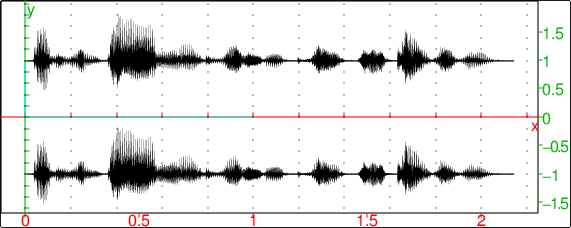
\includegraphics[width=0.75\textwidth]{sound_wav3.png}
\end{center}
Input :
\begin{center}
  \tt clip2:=readwav("/path/to/sounds/example2.wav"):;\\
  plotwav(clip2)
\end{center}
Output :
\begin{center}
  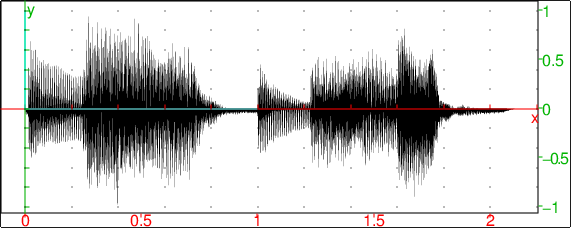
\includegraphics[width=0.75\textwidth]{sound_wav1.png}
\end{center}
Input :
\begin{center}
  \tt plotwav(clip2,range=0.5..0.52)
\end{center}
Output :
\begin{center}
  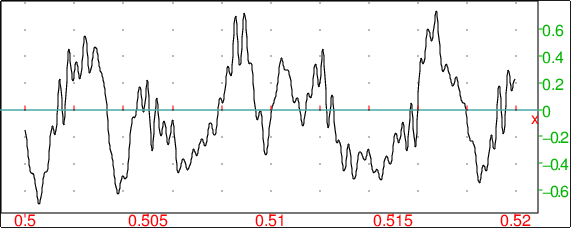
\includegraphics[width=0.75\textwidth]{sound_wav2.png}
\end{center}

\subsection{Visualizing power spectra : {\tt plotspectrum}\index{plotspectrum}}
{\tt plotspectrum} takes an audio clip as its first argument and optionally a range in form {\tt range=[lf,uf]} or {\tt range=lf..uf}, where {\tt lf} is the lower bound and {\tt uf} the upper bound of the desired frequency band, as its second argument. The command displays the power spectrum of the audio data on the specified frequency range (by default $[0,s/2]$, where $s$ is the sampling rate). If the audio clip has more than one channel, the channels are mixed down to a single channel before computing the spectrum.

For example, assume that a male voice is recorded in the file {\tt example1.wav}. Input :
\begin{center}
  \tt clip:=readwav("/path/to/sounds/example1.wav"):;\\
  plotspectrum(clip,range=[0,1500])
\end{center}
Output :
\begin{center}
  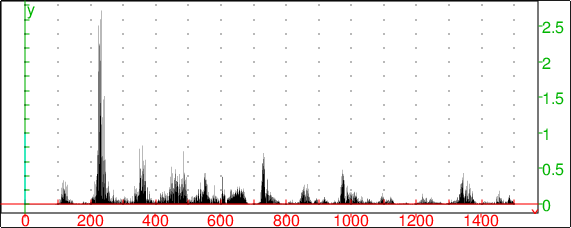
\includegraphics[width=0.75\textwidth]{sound_spectrum.png}
\end{center}
One can observe that the dominant frequency is around 220~Hz, which is the middle of tenor range. This is consistent with the fact that a man is speaking in the clip.

\section{Signal Processing}
\subsection{Boxcar function : {\tt boxcar}\index{boxcar}}\label{sec:boxcar}
The {\tt boxcar} command takes three arguments: real numbers $ a $, $ b $ and an identifier or an expression $ x $. It returns $ u(x-a)-u(x-b) $, where $ u $ is the Heaviside function. The resulting expression defines a function which is zero everywhere except within the segment $ [a,b] $, where its value is equal to 1.

For example, input :
\begin{center}
  \tt boxcar(1,2,x)
\end{center}
Output :
\begin{center}
  \tt Heaviside(x-1)-Heaviside(x-2)
\end{center}
Input :
\begin{center}
  \tt boxcar(1,2,3/2)
\end{center}
Output :
\begin{center}
  \tt 1
\end{center}
Input :
\begin{center}
  \tt boxcar(1,2,0)
\end{center}
Output :
\begin{center}
  \tt 0
\end{center}

\subsection{Rectangle function : {\tt rect}\index{rect}}\label{sec:rect}
The {\tt rect} command takes an identifier or an expression $ x $ and returns the value of the rectangle function at $ x $, which is defined by $ \Pi(x)=u(x+1/2)-u(x-1/2) $ where $ u $ is the Heaviside function. The rectangle function is a special case of boxcar function (see Section~\ref{sec:boxcar}) for $ a=-\frac{1}{2} $ and $ b=\frac{1}{2} $.

For example, input :
\begin{center}
  \tt rect(x/2)
\end{center}
Output :
\begin{center}
  \tt Heaviside(x/2+1/2)-Heaviside(x/2-1/2)
\end{center}

To compute the convolution of the rectangle function with itself, use the convolution theorem. Input :
\begin{center}
  \tt R:=fourier(rect(x),x,s):; ifourier(R\^{}2,s,x)
\end{center}
Output :
\begin{center}
  \tt Heaviside(x+1)-Heaviside(x-1)-2*x*Heaviside(x)+ x*Heaviside(x+1)+x*Heaviside(x-1)
\end{center}
The above result is the triangle function $ \mathrm{tri}(x) $ (see Section~\ref{sec:tri}).

\subsection{Triangle function : {\tt tri}\index{tri}}\label{sec:tri}
The {\tt tri} command takes an expression $ x $ as its only argument and returns the value of triangle function at $ x $, defined by
\[ \Lambda(x)=\begin{cases}1-|x|,&|x|<1,\\0,&\text{otherwise}.\end{cases} \]
The above expression is equal to the convolution of rectangle function with itself (see Section~\ref{sec:rect}).

For example, input :
\begin{center}
  \tt tri(x-1)
\end{center}
Output :
\begin{center}
  \tt x*(Heaviside(-x+1)-Heaviside(-x))+ (Heaviside(x-1)-Heaviside(x-2))*(-x+2)
\end{center}

\subsection{Cardinal sine function : {\tt sinc}\index{sinc}}\label{sec:sinc}
The {\tt sinc} command takes an expression $ x $ as its only argument and returns the value of sinc function at $ x $, defined by
\[ \mathrm{sinc}(x)=\begin{cases}\frac{\sin(x)}{x},&x\neq 0,\\1,&x=0.\end{cases} \]

For example, input :
\begin{center}
  \tt sinc(pi*x)
\end{center}
Output :
\begin{center}
  \tt sin(pi*x)/(pi*x)
\end{center}
Input :
\begin{center}
  \tt sinc(0)
\end{center}
Output :
\begin{center}
  \tt 1
\end{center}

\subsection{Root mean square : {\tt rms}}\index{rms}
{\tt rms} takes one argument, a list $X$ of real or complex numbers $x_1,x_2,\dots,x_n$. The function returns the root mean square of $X$ which is defined by
\[ \operatorname{RMS}(X)=\sqrt{\frac{\sum_{k=1}^n|x_k|^2}{n}}. \]
For example, input :
\begin{center}
	\tt rms([1,2,5,8,3,6,7,9,-1])
\end{center}
Output :
\begin{center}
	\tt sqrt(30)
\end{center}
Input :
\begin{center}
	\tt rms([1,1-i,2+3i,5-2i])
\end{center}
Output :
\begin{center}
	\tt 3*sqrt(5)/2
\end{center}

\subsection{Cross-correlation of two signals : {\tt cross\_correlation}\index{cross\_correlation}}
\label{sec:crosscorr}
{\tt cross\_correlation} takes two arguments, a complex vector $ \mathbf{v} $ of length $ n $ and a complex vector $ \mathbf{w} $ of length $ m $. The returned value is the complex vector $ \mathbf{z}=\mathbf{v}\star\mathbf{w} $ of length $ N=n+m-1 $ which is the cross-correlation of the two input vectors, i.e.~such that the following holds :
\[ z_k=\sum_{i=k}^{N-1}\overline{v_{i-k}^\ast}\,w_i^\ast,\quad k=0,1,\dots,N-1, \]
where
\[ \mathbf{v}^\ast=[v_0,v_1,\dots,v_{n-1},\underbrace{0,0,\dots,0}_{m-1}]\quad\text{and}\quad\mathbf{w}^\ast=[\underbrace{0,0,\dots,0}_{n-1},w_0,w_1,\dots,w_{m-1}]. \]

Cross-correlation is typically used for measuring similarity between signals.

For example, input :
\begin{center}
	\tt cross\_correlation([1,2],[3,4,5])
\end{center}
Output :
\begin{center}
	{\tt [6.0,11.0,14.0,5.0]}
\end{center}
Input :
\begin{center}
  \tt v:=[2,1,3,2]:; w:=[1,-1,1,2,2,1,3,2,1]:;
  round(cross\_correlation(v,w))
\end{center}
Output :
\begin{center}
  \tt [2,1,0,8,9,12,15,18,13,11,5,2]
\end{center}
Observe that the cross-correlation of {\tt v} and {\tt w} is peaking at position 8 with the value 18, indicating that the two signals are best correlated when the last sample in {\tt v} is aligned with the eighth sample in {\tt w}. Indeed, there is an occurrence of {\tt v} in {\tt w} precisely at that point.

\subsection{Auto-correlation of a signal : {\tt auto\_correlation}\index{auto\_correlation}}
{\tt auto\_correlation} takes as argument a complex vector $ \mathbf{v} $ of length $ n $ and returns its cross-correlation with itself as the vector $ \mathbf{v}\star\mathbf{v} $ of length $ 2\,n-1 $ (see the {\tt cross\_correlation} command, section~\ref{sec:crosscorr}). For example, input :
\begin{center}
	{\tt auto\_correlation([2,3,4,3,1,4,5,1,3,1])}
\end{center}
Output :
\begin{center}
	{\tt [2.0,9.0,15.0,28.0,37.0,44.0,58.0,58.0,68.0,\\
		91.0,68.0,58.0,58.0,44.0,37.0,28.0,15.0,9.0,2.0]}
\end{center}

\subsection{Convolution of two signals or functions : {\tt convolution}\index{convolution}}
{\tt convolution} takes two arguments, a real vector $ \mathbf{v} $ of length $ n $ and a real vector $ \mathbf{w} $ of length $ m $, and returns their convolution $ \mathbf{z}=\mathbf{v}\ast\mathbf{w} $ which is the vector of length $ N=n+m-1 $ defined as :
\[ z_k=\sum_{i=0}^{k}v_i\,w_{k-i},\quad k=0,1,\dots,N-1, \]
such that $ v_j=0 $ for $ j\geq n $ and $ w_j=0 $ for $ j\geq m $. The two arguments may also be real functions $ f(x) $ and $ g(x) $, with the variable $ x $ as an optional third argument, in which case the integral
\[ \int_{-\infty}^{+\infty}f(t)\,g(x-t)\,\mathrm{d}t \]
is computed. It is assumed that $ f $ and $ g $ are causal functions, i.e.~$ f(x)=g(x)=0 $ for $ x<0 $. Therefore both $ f $ and $ g $ are multiplied by Heaviside function prior to integration.

For example, input :
\begin{center}
	{\tt convolution([1,2,3],[1,-1,1,-1])}
\end{center}
Output :
\begin{center}
	{\tt [1.0,1.0,2.0,-2.0,1.0,-3.0]}
\end{center}

To compute the convolution of $ f(x)=25\,\mathrm{e}^{2\,x}\,u(x) $ and $ g(x)=x\,\mathrm{e}^{-3\,x}\,u(x) $, where $ u $ is the Heaviside function, input :
\begin{center}
  \tt convolution(25*exp(2x),x*exp(-3x))
\end{center}
Output :
\begin{center}
  \tt Heaviside(x)*(-5*x*exp(-3*x)+exp(2*x)-exp(-3*x))
\end{center}

To compute the convolution of $ f(t)=\ln(1+t)\,u(t) $ and $ g(t)=\frac{1}{\sqrt{t}} $, input :
\begin{center}
  \tt convolution(ln(1+t),1/sqrt(t),t)
\end{center}
Output :
\begin{center}
  \tt 2*Heaviside(t)*((t+1)*ln(abs(sqrt(t)-sqrt(t+1))/(sqrt(t)+sqrt(t+1)))+ 2*sqrt(t\^{}2+t))/sqrt(t+1)
\end{center}

In the following example convolution is used for reverberation. Assume that the directory {\tt sounds} contains two files, a dry, mono recording of a guitar stored in {\tt guitar.wav} and a two-channel impulse response recorded in a French 18th century salon and stored in {\tt salon-ir.wav}. Files are loaded with the following command lines :
\begin{center}
  \tt clip:=readwav("/path/to/sounds/guitar.wav"):; ir:=readwav("/path/to/sounds/salon-ir.wav"):;
\end{center}
Input :
\begin{center}
  \tt plotwav(clip)
\end{center}
Output :
\begin{center}
  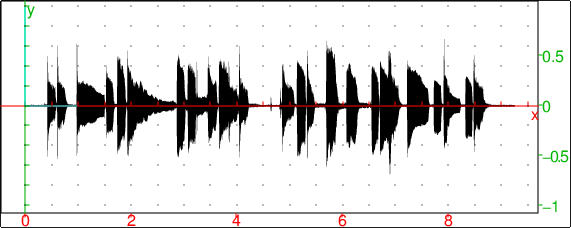
\includegraphics[width=0.75\textwidth]{sound_guitar.png}
\end{center}
Input :
\begin{center}
  \tt plotwav(ir)
\end{center}
Output :
\begin{center}
  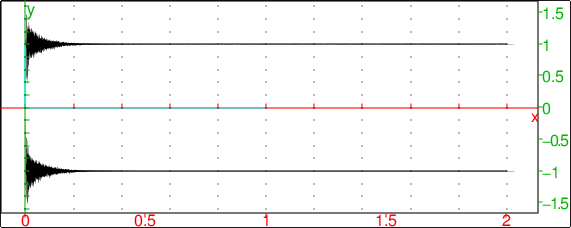
\includegraphics[width=0.75\textwidth]{sound_salon.png}
\end{center}
Convolving the data from {\tt clip} with both channels in {\tt ir} produces a reverberated variant of the recording, in stereo. Input :
\begin{center}
  \tt data:=channel\_data(clip):; L:=convolution(data,channel\_data(ir,1)):; R:=convolution(data,channel\_data(ir,2)):;
\end{center}
The convolved signals {\tt L} and {\tt R} now become the left and right channel of a new audio clip, respectively. The {\tt normalize} option is used because convolution usually results in a huge increase of sample values (which is clear from the definition). Input :
\begin{center}
  \tt spatial:=createwav([L,R],normalize=-3):; playsnd(spatial)
\end{center}
The result sounds as it was recorded in the same salon as the impulse response. Furthermore, it is a true stereo sound. To visualize it, input :
\begin{center}
  \tt plotwav(spatial)
\end{center}
Output :
\begin{center}
  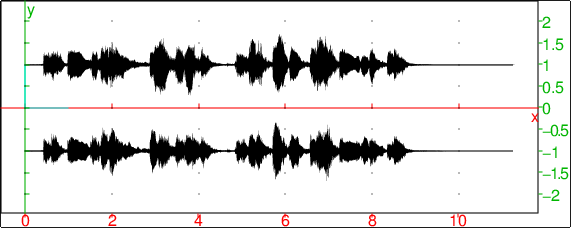
\includegraphics[width=0.75\textwidth]{sound_reverb.png}
\end{center}
Note that the resulting audio is longer than the input (for the length of the impulse response).

\subsection{Low-pass filtering : {\tt lowpass}\index{lowpass}}
{\tt lowpass} takes two or three arguments: an audio clip or a real vector $ \mathbf{v} $ representing the sampled signal, a real number $ c $ specifying the cutoff frequency and optionally a samplerate (which defaults to 44100). The command returns the input data after applying a simple first-order lowpass RC filter.

For example, input :
\begin{center}
	{\tt f:=unapply(periodic(sign(x),x,-1/880,1/880),x);\\
		s:=apply(f,soundsec(3)):;\\
		playsnd(lowpass(createwav(s),1000))}
\end{center}

\subsection{High-pass filtering : {\tt highpass}\index{highpass}}
{\tt highpass} takes two or three arguments: an audio clip or a real vector $ \mathbf{v} $ representing the sampled signal, a real number $ c $ specifying the cutoff frequency and optionally a samplerate (which defaults to 44100). The command returns the input data after applying a simple first-order highpass RC filter.

For example, input :
\begin{center}
	{\tt f:=unapply(periodic(sign(x),x,-1/880,1/880),x);\\
		s:=apply(f,soundsec(3)):;\\
		playsnd(highpass(createwav(s),5000))}
\end{center}

\subsection{Apply a moving average filter to a signal : {\tt moving\_average\index{moving\_average}}}
{\tt moving\_average} takes two arguments: an array $A$ of numeric values representing the sampled signal and a positive integer $n$. It returns an array $B$ obtained by applying a moving average filter of length $n$ to $A$. The elements of $B$ are defined by
\[ B[i]=\frac{1}{n}\,\sum_{j=0}^{n-1}A[i+j] \]
for $i=0,1,\dots,L-n$, where $L$ is the length of $A$.

Moving average filters are fast and useful for smoothing time-encoded signals. For example, input :
\begin{center}
  {\tt snd:=soundsec(2):;\\
  noise:=randvector(length(snd),normald,0,0.05):;\\
  data:=0.5*threshold(3*sin(2*pi*220*snd),[-1.0,1.0])+noise:;\\
  plotwav(createwav(data),range=[1000,1500])}
\end{center}
Output :
\begin{center}
  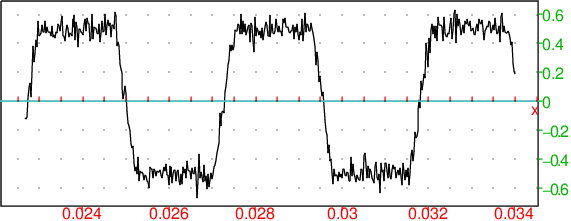
\includegraphics[width=0.75\textwidth]{signalproc_mavg1.png}
\end{center}
Input :
\begin{center}
  {\tt fdata:=moving\_average(data,25):;\\
  plotwav(createwav(fdata),range=[1000,1500])}
\end{center}
Output :
\begin{center}
  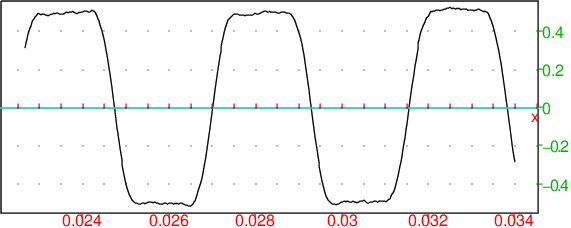
\includegraphics[width=0.75\textwidth]{signalproc_mavg2.png}
\end{center}

\subsection{Perform thresholding operations on an array : {\tt threshold}\index{threshold}}
{\tt threshold} changes the data in an array which does not meet some kind of minimality criterion. It takes the following parameters :
\begin{itemize}
	\item vector $ \mathbf{v} $ of real or complex numbers
	\item bound specification {\tt bnd}
	\item comparison operator (optional)
	\item {\tt abs[=true,false]} (optional)
\end{itemize}
Bound specification may be either a single real number $ b $ (or an equation {\tt b=value}) or a list of two real numbers $ l,u $ (or equations {\tt l=lvalue}, {\tt u=uvalue}). In the latter case a vector $ \mathbf{w} $ is returned, as defined by :
\[ w_k=\begin{cases}
\text{{\tt uvalue} (defaults to $ u $)},&v_k>u,\\
\text{{\tt lvalue} (defaults to $ l $)},&v_k<l,\\
v_k,&\text{otherwise}
\end{cases} \]
for $ k=0,1,\dots,n-1 $ where $ n= ${\tt size}($ \mathbf{v} $) when the element $ v_k $ is a real number. If $ v_k $ is complex, then $ |v_k| $ is compared with $ u $ resp.~$ l $ and the value {\tt uvalue} resp.~{\tt lvalue} is multiplied by $ \frac{v_k}{|v_k|} $.

In the first case where {\tt bnd} is a number or an equation, the return vector $ \mathbf{w} $ is defined by :
\[ w_k=\begin{cases}
\text{{\tt value} (defaults to $ b $)},&v_k<b,\\
v_k,&\text{otherwise}
\end{cases} \]
if $ v_k\in\mathbb{R} $ (if $ v_k $ is complex, then $ |v_k| $ is compared with $ b $ and the {\tt value} is multiplied by $ \frac{v_k}{|v_k|} $), for $ k=0,1,\dots,n-1 $. If comparison operator is specified (one of {\tt >}, {\tt <=} or {\tt >=}, must be quoted), it is used instead of {\tt <} (which is the default) in the above formula. If the fourth argument is specified, the data in $ \mathbf{v} $ must be real and the following formula is used for $ w_k $, $ k=0,1,\dots,n-1 $ :
\[ w_k=\begin{cases}
\text{{\tt value}},& \text{$ v_k\geq 0 $ and $ |v_k|<b $},\\
-\text{{\tt value}},& \text{$ v_k<0 $ and $ |v_k|<b $},\\
v_k,&\text{otherwise}.
\end{cases} \]
As before, {\tt value} defaults to $ b $ and the comparison operator used to test $ |v_k| $ against $ b $ (by default {\tt <}) is specified by the third argument.

For example, input :
\begin{center}
	{\tt threshold([2,3,1,2,5,4,3,7],3)}
\end{center}
Output :
\begin{center}
	{\tt [3,3,3,3,5,4,3,7]}
\end{center}
Input :
\begin{center}
	{\tt threshold([2,3,1,2,5,4,3,7],3=a,'>=')}
\end{center}
Output :
\begin{center}
	{\tt [2,a,1,2,a,a,a,a]}
\end{center}
Input :
\begin{center}
	{\tt threshold([-2,-3,1,2,5,-4,3,-1],3=0,abs=true)}
\end{center}
Output :
\begin{center}
	{\tt [0,-3,0,0,5,-4,3,0]}
\end{center}
Input :
\begin{center}
	{\tt threshold([-2,-3,1,2,5,-4,3,-1],3=0,'<=',abs=true)}
\end{center}
Output :
\begin{center}
	{\tt [0,0,0,0,5,-4,0,0]}
\end{center}
Input :
\begin{center}
	{\tt threshold([-120,-11,-3,0,7,27,111,234],[-100,100])}
\end{center}
Output :
\begin{center}
	{\tt [-100,-11,-3,0,7,27,100,100]}
\end{center}
Input :
\begin{center}
	{\tt threshold([-120,-11,-3,0,7,27,111,234],[-100=-inf,100=inf])}
\end{center}
Output :
\begin{center}
	{\tt [-infinity,-11,-3,0,7,27,+infinity,+infinity]}
\end{center}

In the following example, a square-like wave is created from a single sine wave by clipping sample values. Input :
\begin{center}
  \tt data:=threshold(3*sin(2*pi*440*soundsec(2)),[-1.0,1.0]):;\\s:=createwav(data):; playsnd(s)
\end{center}
Output :
\begin{center}
  \tt 1
\end{center}
Input :
\begin{center}
  \tt plotwav(s,range=[1000,2000])
\end{center}
Output :
\begin{center}
  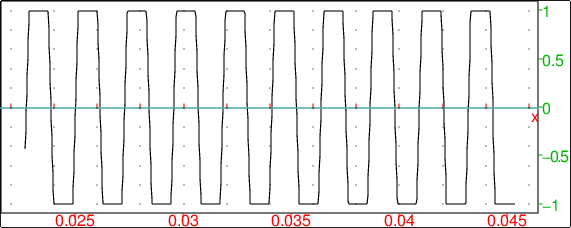
\includegraphics[width=0.75\textwidth]{sound_wav4.png}
\end{center}

\subsection{Bartlett-Hann window function : {\tt bartlett\_hann\_window}\index{bartlett\_hann\_window}}
{\tt bartlett\_hann\_window} takes as arguments a real vector $ \mathbf{v} $ of length $ n $ and optionally an interval $ n_1 ${\tt ..}$ n_2 $ (with default values $ n_1=0 $ and $ n_2=n-1 $), and returns the elementwise product of the vector $ [v_{n_1},\dots,v_{n_2}] $ and the vector $ \mathbf{w} $ of length $ N=n_2-n_1+1 $ defined by
\[ w_k=a_0+a_1\,\left|\frac{k}{N-1}-\frac{1}{2}\right|-a_2\,\cos\left(\frac{2\,k\,\pi}{N-1}\right) \]
for $ k=0,1,\dots,N-1 $, where $ a_0=0.62 $, $ a_1=0.48 $ and $ a_2=0.38 $. For example, input :
\begin{center}
	{\tt L:=bartlett\_hann\_window(randvector(1000,0..1)):;}
\end{center}
followed by {\tt scatterplot(L)}.

\subsection{Blackman-Harris window function : {\tt blackman\_harris\_window}\index{blackman\_harris\_window}}
{\tt blackman\_harris\_window} takes as arguments a real vector $ \mathbf{v} $ of length $ n $ and optionally an interval $ n_1 ${\tt ..}$ n_2 $ (with default values $ n_1=0 $ and $ n_2=n-1 $), and returns the elementwise product of the vector $ [v_{n_1},\dots,v_{n_2}] $ and the vector $ \mathbf{w} $ of length $ N=n_2-n_1+1 $ defined by
\[ w_k=a_0-a_1\,\cos\left(\frac{2\,k\,\pi}{N-1}\right)+a_2\,\cos\left(\frac{4\,k\,\pi}{N-1}\right)-a_3\,\cos\left(\frac{6\,k\,\pi}{N-1}\right) \]
for $ k=0,1,\dots,N-1 $, where $ a_0=0.35875 $, $ a_1=0.48829 $, $ a_2=0.14128 $ and $ a_3=0.01168 $. For example, input :
\begin{center}
	{\tt L:=blackman\_harris\_window(randvector(1000,0..1)):;}
\end{center}
followed by {\tt scatterplot(L)}.

\subsection{Blackman window function : {\tt blackman\_window}\index{blackman\_window}}
{\tt blackman\_window} takes as arguments a real vector $ \mathbf{v} $ of length $ n $ and optionally a real number $ \alpha $ (by default $ \alpha=0.16 $) and/or an interval $ n_1 ${\tt ..}$ n_2 $ (with default values $ n_1=0 $ and $ n_2=n-1 $), and returns the elementwise product of the vector $ [v_{n_1},\dots,v_{n_2}] $ and the vector $ \mathbf{w} $ of length $ N=n_2-n_1+1 $ defined by
\[ w_k=\frac{1-\alpha}{2}-\frac{1}{2}\,\cos\left(\frac{2\,k\,\pi}{N-1}\right)+\frac{\alpha}{2}\,\cos\left(\frac{4\,k\,\pi}{N-1}\right) \]
for $ k=0,1,\dots,N-1 $. For example, input :
\begin{center}
	{\tt L:=blackman\_window(randvector(1000,0..1)):;}
\end{center}
followed by {\tt scatterplot(L)}.

\subsection{Bohman window function : {\tt bohman\_window}\index{bohman\_window}}
{\tt bohman\_window} takes as arguments a real vector $ \mathbf{v} $ of length $ n $ and optionally an interval $ n_1 ${\tt ..}$ n_2 $ (with default values $ n_1=0 $ and $ n_2=n-1 $), and returns the elementwise product of the vector $ [v_{n_1},\dots,v_{n_2}] $ and the vector $ \mathbf{w} $ of length $ N=n_2-n_1+1 $ defined by
\[ w_k=\left(1-x_k\right)\,\cos\left(\pi\,x_k\right)+\frac{1}{\pi}\,\sin\left(\pi\,x_k\right), \]
where $ x_k=\left|\frac{2\,k}{N-1}-1\right| $, for $ k=0,1,\dots,N-1 $. For example, input :
\begin{center}
	{\tt L:=bohman\_window(randvector(1000,0..1)):;}
\end{center}
followed by {\tt scatterplot(L)}.

\subsection{Cosine window function : {\tt cosine\_window}\index{cosine\_window}}
{\tt cosine\_window} takes as arguments a real vector $ \mathbf{v} $ of length $ n $ and optionally a positive real number $ \alpha $ (by default $ \alpha=1 $) and/or an interval $ n_1 ${\tt ..}$ n_2 $ (with default values $ n_1=0 $ and $ n_2=n-1 $), and returns the elementwise product of the vector $ [v_{n_1},\dots,v_{n_2}] $ and the vector $ \mathbf{w} $ of length $ N=n_2-n_1+1 $ defined by
\[ w_k=\sin^\alpha\left(\frac{k\,\pi}{N-1}\right) \]
for $ k=0,1,\dots,N-1 $. For example, input :
\begin{center}
	{\tt L:=cosine\_window(randvector(1000,0..1),1.5):;}
\end{center}
followed by {\tt scatterplot(L)}.

\subsection{Gaussian window function : {\tt gaussian\_window}\index{gaussian\_window}}
{\tt gaussian\_window} takes as arguments a real vector $ \mathbf{v} $ of length $ n $ and optionally a positive real number $ \alpha\leq 0.5 $ (by default $ \alpha=0.1 $) and/or an interval $ n_1 ${\tt ..}$ n_2 $ (with default values $ n_1=0 $ and $ n_2=n-1 $), and returns the elementwise product of the vector $ [v_{n_1},\dots,v_{n_2}] $ and the vector $ \mathbf{w} $ of length $ N=n_2-n_1+1 $ defined by
\[ w_k=\exp\left(-\frac{1}{2}\,\left(\frac{k-(N-1)/2}{\alpha\,(N-1)/2}\right)^2\right) \]
for $ k=0,1,\dots,N-1 $. For example, input :
\begin{center}
	{\tt L:=gaussian\_window(randvector(1000,0..1),0.4):;}
\end{center}
followed by {\tt scatterplot(L)}.

\subsection{Hamming window function : {\tt hamming\_window}\index{hamming\_window}}
{\tt hamming\_window} takes as arguments a real vector $ \mathbf{v} $ of length $ n $ and optionally an interval $ n_1 ${\tt ..}$ n_2 $ (with default values $ n_1=0 $ and $ n_2=n-1 $), and returns the elementwise product of the vector $ [v_{n_1},\dots,v_{n_2}] $ and the vector $ \mathbf{w} $ of length $ N=n_2-n_1+1 $ defined by
\[ w_k=\alpha-\beta\,\cos\left(\frac{2\,k\,\pi}{N-1}\right) \]
for $ k=0,1,\dots,N-1 $, where $ \alpha=0.54 $ and $ \beta=1-\alpha=0.46 $. For example, input :
\begin{center}
	{\tt L:=hamming\_window(randvector(1000,0..1)):;}
\end{center}
followed by {\tt scatterplot(L)}.

\subsection{Hann-Poisson window function : {\tt hann\_poisson\_window}\index{hann\_poisson\_window}}
{\tt hann\_poisson\_window} takes as arguments a real vector $ \mathbf{v} $ of length $ n $ and optionally a real number $ \alpha $ (by default $ \alpha=1 $) and/or an interval $ n_1 ${\tt ..}$ n_2 $ (with default values $ n_1=0 $ and $ n_2=n-1 $), and returns the elementwise product of the vector $ [v_{n_1},\dots,v_{n_2}] $ and the vector $ \mathbf{w} $ of length $ N=n_2-n_1+1 $ defined by
\[ w_k=\frac{1}{2}\,\left(1-\cos\frac{2\,k\,\pi}{N-1}\right)\,\exp\left(-\frac{\alpha\,|N-1-2\,k|}{N-1}\right) \]
for $ k=0,1,\dots,N-1 $. For example, input :
\begin{center}
	{\tt L:=hann\_poisson\_window(randvector(1000,0..1),2):;}
\end{center}
followed by {\tt scatterplot(L)}.

\subsection{Hann window function : {\tt hann\_window}\index{hann\_window}}
{\tt hann\_window} takes as arguments a real vector $ \mathbf{v} $ of length $ n $ and optionally an interval $ n_1 ${\tt ..}$ n_2 $ (with default values $ n_1=0 $ and $ n_2=n-1 $), and returns the elementwise product of the vector $ [v_{n_1},\dots,v_{n_2}] $ and the vector $ \mathbf{w} $ of length $ N=n_2-n_1+1 $ defined by
\[ w_k=\sin^2\left(\frac{k\,\pi}{N-1}\right) \]
for $ k=0,1,\dots,N-1 $. For example, input :
\begin{center}
	{\tt L:=hann\_window(randvector(1000,0..1)):;}
\end{center}
followed by {\tt scatterplot(L)}.

\subsection{Parzen window function : {\tt parzen\_window}\index{parzen\_window}}
{\tt parzen\_window} takes as arguments a real vector $ \mathbf{v} $ of length $ n $ and optionally an interval $ n_1 ${\tt ..}$ n_2 $ (with default values $ n_1=0 $ and $ n_2=n-1 $), and returns the elementwise product of the vector $ [v_{n_1},\dots,v_{n_2}] $ and the vector $ \mathbf{w} $ of length $ N=n_2-n_1+1 $ defined by
\[ w_k=\begin{cases}
\left(1-6\,x_k^2\,\left(1-x_k\right)\right),&\left|\frac{N-1}{2}-k\right|\leq\frac{N-1}{4},\\
2\,\left(1-x_k\right)^3,&\text{otherwise},
\end{cases} \]
where $ x_k=\left|1-\frac{2\,k}{N-1}\right| $, for $ k=0,1,\dots,N-1 $. For example, input :
\begin{center}
	{\tt L:=parzen\_window(randvector(1000,0..1)):;}
\end{center}
followed by {\tt scatterplot(L)}.

\subsection{Poisson window function : {\tt poisson\_window}\index{poisson\_window}}
{\tt poisson\_window} takes as arguments a real vector $ \mathbf{v} $ of length $ n $ and optionally a real number $ \alpha $ (by default $ \alpha=1 $) and/or an interval $ n_1 ${\tt ..}$ n_2 $ (with default values $ n_1=0 $ and $ n_2=n-1 $), and returns the elementwise product of the vector $ [v_{n_1},\dots,v_{n_2}] $ and the vector $ \mathbf{w} $ of length $ N=n_2-n_1+1 $ defined by
\[ w_k=\exp\left(-\alpha\,\left|\frac{2\,k}{N-1}-1\right|\right) \]
for $ k=0,1,\dots,N-1 $. For example, input :
\begin{center}
	{\tt L:=poisson\_window(randvector(1000,0..1),2):;}
\end{center}
followed by {\tt scatterplot(L)}.

\subsection{Riemann window function : {\tt riemann\_window}\index{riemann\_window}}
{\tt riemann\_window} takes as arguments a real vector $ \mathbf{v} $ of length $ n $ and optionally an interval $ n_1 ${\tt ..}$ n_2 $ (with default values $ n_1=0 $ and $ n_2=n-1 $), and returns the elementwise product of the vector $ [v_{n_1},\dots,v_{n_2}] $ and the vector $ \mathbf{w} $ of length $ N=n_2-n_1+1 $ defined by
\[ w_k=\begin{cases}
1,&k=\frac{N-1}{2},\\
\frac{\sin(\pi\,x_k)}{\pi\,x_k},&\text{otherwise},
\end{cases} \]
where $ x_k=\frac{2\,k}{N-1}-1 $, for $ k=0,1,\dots,N-1 $. For example, input :
\begin{center}
	{\tt L:=riemann\_window(randvector(1000,0..1)):;}
\end{center}
followed by {\tt scatterplot(L)}.

\subsection{Triangular window function : {\tt triangle\_window}\index{triangle\_window}}
{\tt triangle\_window} takes as arguments a real vector $ \mathbf{v} $ of length $ n $ and optionally an integer $ d\in\{-1,0,1\} $ (by default $ d=0 $) and/or an interval $ n_1 ${\tt ..}$ n_2 $ (with default values $ n_1=0 $ and $ n_2=n-1 $), and returns the elementwise product of the vector $ [v_{n_1},\dots,v_{n_2}] $ and the vector $ \mathbf{w} $ of length $ N=n_2-n_1+1 $ defined by
\[ w_k=1-\left|\frac{n-\frac{N-1}{2}}{\frac{N+d}{2}}\right| \]
for $ k=0,1,\dots,N-1 $ (the case $ d=-1 $ is called the Bartlett window function). For example, input :
\begin{center}
	{\tt L:=triangle\_window(randvector(1000,0..1),1):;}
\end{center}
followed by {\tt scatterplot(L)}.

\subsection{Tukey window function : {\tt tukey\_window}\index{tukey\_window}}
{\tt tukey\_window} takes as arguments a real vector $ \mathbf{v} $ of length $ n $ and optionally a real number $ \alpha\in[0,1] $ (by default $ \alpha=0.5 $) and/or an interval $ n_1 ${\tt ..}$ n_2 $ (with default values $ n_1=0 $ and $ n_2=n-1 $), and returns the elementwise product of the vector $ [v_{n_1},\dots,v_{n_2}] $ and the vector $ \mathbf{w} $ of length $ N=n_2-n_1+1 $ defined by
\[ w_k=\begin{cases}
\frac{1}{2}\,\left(1+\cos\left(\pi\,\left(\frac{k}{\beta}-1\right)\right)\right),&k<\beta,\\
1,&\beta\leq k\leq(N-1)\,\left(1-\frac{\alpha}{2}\right),\\
\frac{1}{2}\,\left(1+\cos\left(\pi\,\left(\frac{k}{\beta}-\frac{2}{\alpha}+1\right)\right)\right),&\text{otherwise},
\end{cases} \]
where $ \beta=\frac{\alpha\,(N-1)}{2} $, for $ k=0,1,\dots,N-1 $. When $ \alpha=0 $ the rectangular window function (on-off windowing) is obtained, and the case $ \alpha=1 $ corresponds to the Hann window function. For example, input :
\begin{center}
	{\tt L:=tukey\_window(randvector(1000,0..1),0.4):;}
\end{center}
followed by {\tt scatterplot(L)}.

\subsection{Welch window function : {\tt welch\_window}\index{welch\_window}}
{\tt welch\_window} takes as arguments a real vector $ \mathbf{v} $ of length $ n $ and optionally an interval $ n_1 ${\tt ..}$ n_2 $ (with default values $ n_1=0 $ and $ n_2=n-1 $), and returns the elementwise product of the vector $ [v_{n_1},\dots,v_{n_2}] $ and the vector $ \mathbf{w} $ of length $ N=n_2-n_1+1 $ defined by
\[ w_k=1-\left(\frac{k-\frac{N-1}{2}}{\frac{N-1}{2}}\right)^2 \]
for $ k=0,1,\dots,N-1 $. For example, input :
\begin{center}
	{\tt L:=welch\_window(randvector(1000,0..1)):;}
\end{center}
followed by {\tt scatterplot(L)}.

\subsection{An example : static noise removal\index{noise removal} by spectral subtraction}
In this section we use Xcas to inplement a simple algorithm for static noise removal based on the spectral subtraction method. For a theoretical overview see the paper "Noise Reduction Based on Modified Spectral Subtraction Method" by Ekaterina Verteletskaya and Boris Simak (2011), \emph{International Journal of Computer Science}, 38:1 (\href{https://pdfs.semanticscholar.org/c212/84207dcf8e95b8b44d0ce703f9fe23b28f2a.pdf}{PDF}).

Efficiency of the spectral subtraction method is largely dependent on a good noise spectrum estimate. Below is the code for a function {\tt noiseprof} that takes {\tt data} and {\tt wlen} as its arguments. These are, respectively, a signal chunk containing only noise and the window length for signal segmentation (the best values are powers of two, such as 256, 512 or 1024). The function returns an estimate of the noise power spectrum obtained by averaging the power spectra of a (not too large) number of distinct chunks of {\tt data} of length {\tt wlen}. Hamming window function is applied prior to FFT.
\begin{verbatim}
noiseprof(data,wlen):={
  local N,h,dx,x,v,cnt;
  N:=length(data);
  h:=wlen/2;
  dx:=min(h,max(1,(N-wlen)/100));
  v:=[0$wlen];
  cnt:=0;
  for (x:=h;x<N-h;x+=dx) {
    v+=abs(fft(hamming_window(
                 mid(data,floor(x)-h,wlen)))).^2;
    cnt++;
  };
  return 1.0/cnt*v;
}:;
\end{verbatim}

The main function is {\tt noisered}, which takes three arguments: the input signal {\tt data}, the noise power spectrum {\tt np} and the "spectral floor" parameter {\tt beta} ($\beta$, the minimum power level). The function performs subtraction of the noise spectrum in chunks of length {\tt wlen} (the length of list {\tt np}) using the overlap-and-add approach with Hamming window function. For details see Section 3A of the paper "Speech Enhancement using Spectral Subtraction-type Algorithms: A Comparison and Simulation Study" by Navneet Upadhyay and Abhijit Karmakar (2015), \emph{Procedia Computer Science}, vol.~54, pp.~574--584 (\href{https://core.ac.uk/download/pdf/81218023.pdf}{PDF}).
\begin{verbatim}
noisered(data,np,beta):={
  local wlen,h,N,L,padded,out,j,k,s,ds,r,alpha;
  wlen:=length(np);
  N:=length(data);
  h:=wlen/2;
  L:=0;
  repeat L+=wlen; until L>=N;
  padded:=concat(data,[0$(L-N)]);
  out:=[0$L];
  for (k:=0;k<L-wlen;k+=h) {
    s:=fft(hamming_window(mid(padded,k,wlen)));
    alpha:=max(1,4-3*sum(abs(s).^2)/(20*sum(np)));
    r:=ifft(zip(max,abs(s).^2-alpha*np,beta*np).^(1/2)
            .*exp(i*arg(s)));
    for (j:=0;j<wlen;j++) {
      out[k+j]+=re(r[j]);
    };
  };
  return mid(out,0,N);
}:;
\end{verbatim}

To demonstrate the efficiency of the algorithm, we test it on a small speech sample with an audible amount of static noise. Assume that the corresponding WAV file {\tt noised.wav} is stored in the directory {\tt sounds}. Input :
\begin{center}
  \tt clip:=readwav("/path/to/sounds/noised.wav"):; plotwav(clip)
\end{center}
Output :
\begin{center}
  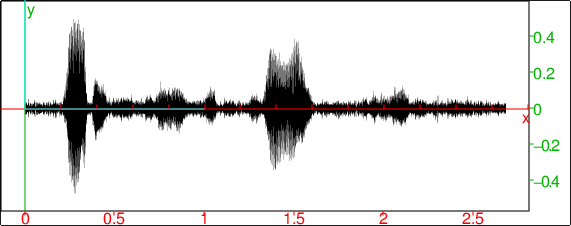
\includegraphics[width=0.75\textwidth]{sound_noise.png}
\end{center}
Speech starts after approximately 0.2 seconds of pure noise. We use that part of the clip for obtaining an estimate of the noise power spectrum with {\tt wlen} set to 256. Input :
\begin{center}
  \tt noise:=channel\_data(clip,range=0.0..0.15):; np:=noiseprof(noise,256):;
\end{center}
Now we call the {\tt noisered} function with $\beta=0.03$ :
\begin{center}
  \tt c:=noisered(channel\_data(clip),np,0.03):; cleaned:=createwav(c):; plotwav(cleaned)
\end{center}
Output :
\begin{center}
  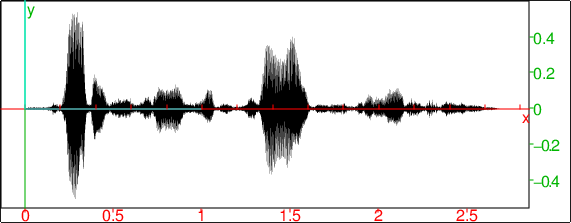
\includegraphics[width=0.75\textwidth]{sound_clean.png}
\end{center}
It is clearly visible that the noise level is significantly lower than in the original clip. One can also use the {\tt playsnd} command to compare the input with the output by hearing, which reveals that the noise is still present but in a lesser degree (the parameter $\beta$ controls how much noise is "left in").

The algorithm implemented in this section is not particularly fast (removing the noise from a two and a half seconds long recording took 20 seconds of computation time), but serves as a proof of concept and demonstrates the efficiency of noise removal.

%%%%%%%%%%%%%%%%%%%%%%%%%%%%%%

\section{Exponentials and Logarithms}
\subsection{Rewrite hyperbolic functions as exponentials : {\tt hyp2exp}}\index{hyp2exp}
\noindent{\tt hyp2exp} takes as argument an hyperbolic expression.\\
{\tt hyp2exp} rewrites each hyperbolic functions with exponentials
(as a rational fraction of one exponential,
i.e. {\sc without} linearization).\\ 
Input :
\begin{center}{\tt hyp2exp(sinh(x))}\end{center}
Output :
\begin{center}{\tt (exp(x)-1/(exp(x)))/2}\end{center}

\subsection{Expand exponentials : {\tt expexpand}}\index{expexpand}
\noindent{\tt expexpand} takes as argument an expression with exponentials.\\
{\tt expexpand} expands this expression (rewrites exp of sums as
product of exp).\\
Input :
\begin{center}{\tt expexpand(exp(3*x)+exp(2*x+2))}\end{center}
Output :
\begin{center}{\tt exp(x)\verb|^|3+exp(x)\verb|^|2*exp(2)}\end{center}

\subsection{Expand logarithms : {\tt lnexpand}}\index{lnexpand}
\noindent{\tt lnexpand} takes as argument an expression with logarithms.\\
{\tt lnexpand} expands this expression (rewrites ln of products
as sum of ln).\\
Input :
\begin{center}{\tt lnexpand(ln(3*x\verb|^|2)+ln(2*x+2))}\end{center}
Output :
\begin{center}{\tt  ln(3)+2*ln(x)+ln(2)+ln(x+1)}\end{center}

\subsection{Linearize exponentials : {\tt lin}}\index{lin}
\noindent{\tt lin} takes as argument an expression with
exponentials.\\
{\tt lin} rewrites hyperbolic functions as exponentials if required,
then linearizes this expression (i.e. replace product of
exponentials by exponential of sums).\\
{\bf Examples}
\begin{itemize}
\item Input :
\begin{center}{\tt lin(sinh(x)\verb|^|2)}\end{center}
Output :
\begin{center}{\tt 1/4*exp(2*x)+1/-2+1/4*exp(-(2*x))}\end{center}

\item Input :
\begin{center}{\tt lin((exp(x)+1)\verb|^|3)}\end{center}
Output :
\begin{center}{\tt exp(3*x)+3*exp(2*x)+3*exp(x)+1}\end{center}
\end{itemize}

\subsection{Collect logarithms : {\tt lncollect}}\index{lncollect}
\noindent{\tt lncollect} takes as argument an expression with logarithms.\\
{\tt lncollect} collects the logarithms (rewrites sum of ln
as ln of products). 
It may be a good idea to factor the 
expression with {\tt factor} before collecting by {\tt lncollect}).\\
Input :
\begin{center}{\tt lncollect(ln(x+1)+ln(x-1))}\end{center}
Output :
\begin{center}{\tt log((x+1)*(x-1))}\end{center}
Input :
\begin{center}{\tt lncollect(exp(ln(x+1)+ln(x-1)))}\end{center}
Output :
\begin{center}{\tt (x+1)*(x-1)}\end{center}
{\bf Warning!!!}  For {\tt Xcas}, {\tt log=ln} (use {\tt log10}
for 10-base logarithm).

\subsection{Expand powers : {\tt powexpand}}\index{powexpand}
\noindent{\tt powexpand} rewrites a power of a sum as a product of powers.\\
Input :
\begin{center}{\tt powexpand(a\verb|^|(x+y))}\end{center}
Output :
\begin{center}{\tt a\verb|^|x*a\verb|^|y}\end{center}


\subsection{Rewrite a power as an exponential : {\tt pow2exp}}\index{pow2exp}
\noindent{\tt pow2exp} rewrites a power as an exponential.\\
Input :
\begin{center}{\tt  pow2exp(a\verb|^|(x+y))}\end{center}
Output :
\begin{center}{\tt exp((x+y)*ln(a))}\end{center}

\subsection{Rewrite exp(n*ln(x)) as a power : {\tt exp2pow}}\index{exp2pow}
\noindent{\tt exp2pow} rewrites expression of the form $\exp(n*\ln(x))$
as a power of $x$.\\
Input :
\begin{center}{\tt  exp2pow(exp(n*ln(x)))}\end{center}
Output :
\begin{center}{\tt x\verb|^|n}\end{center}
Note the difference with {\tt lncollect} :\\
{\tt lncollect(exp(n*ln(x))) = exp(n*log(x))}\\
{\tt lncollect(exp(2*ln(x))) = exp(2*log(x))}\\
{\tt exp2pow(exp(2*ln(x))) = x\verb|^|2 }\\
But :\\
{\tt lncollect(exp(ln(x)+ln(x))) = x\verb|^|2}\\
{\tt exp2pow(exp(ln(x)+ln(x))) = x\verb|^|(1+1)}\\

\subsection{Simplify complex exponentials : {\tt tsimplify}}\index{tsimplify}
\noindent{\tt tsimplify} simplifies transcendental expressions 
by rewriting the expression with complex exponentials.\\
It is a good idea to try other simplification instructions
and call {\tt tsimplify} if they do not work.\\ 
Input :
\begin{center}{\tt tsimplify((sin(7*x)+sin(3*x))/sin(5*x))}\end{center}
Output :
\begin{center}{\tt ((exp((i)*x))\verb|^|4+1)/(exp((i)*x))\verb|^|2 }\end{center}

\section{Polynomials}
\label{sec:polynomials}

\subsection{Polynomials of a single variable: \texttt{poly1}}
\index{poly1}
A polynomial of one variable is represented either 
by a symbolic expression or by the list of its 
coefficients in decreasing powers order (dense representation).
In the latter case, to avoid confusion with other kinds of list
\begin{itemize}
\item use \verb|poly1[...]| as delimiters in inputs
\item check for $\talloblong \ \talloblong$ in {\tt Xcas} output.
\end{itemize}
Note that polynomials represented as lists of coefficients
are always written in decreasing powers order even if  
{\tt increasing power} is checked in  {\tt cas} configuration.

\subsection{Polynomials of several variables: 
\texttt{\%\%\%\{ \%\%\%\}}}
\index{\%\%\%\{ \%\%\%\}}

A polynomial of several variables is represented
\begin{itemize}
\item by a symbolic expression 
\item or by a dense recursive 1-d representation like above
\item or by a sum of
monomials with non-zero coefficients (distributed sparse
representation).\\
A monomial with several variables is represented by a coefficient and a
list of integers (interpreted as powers of a variable list). The 
delimiters for monomials are
{\tt \%\%\%\{} and  {\tt \%\%\%\}}, for example $3x^2y$ is represented by
{\tt \%\%\%\{3,[2,1]\%\%\%\}} with respect to the variable list 
{\tt [x,y]}).
\end{itemize} 

\subsection{Convert to a symbolic polynomial : {\tt r2e poly2symb}}\index{r2e}\index{poly2symb}
\noindent{\tt r2e} or  {\tt poly2symb} takes as argument 
\begin{itemize}
\item a list of 
coefficients of a polynomial (by decreasing order) and a symbolic
variable name 
(by default {\tt x})
\item or a sum of monomials {\tt \%\%\%\{coeff,[n1,....nk] \%\%\%\}} 
and a vector of symbolic variables {\tt [x1,...,xk]}.
\end{itemize}
{\tt r2e} or  {\tt poly2symb} transforms the argument into a symbolic
polynomial.\\
Example with univariate polynomials, input :
\begin{center}{\tt r2e([1,0,-1],x)}\end{center}
or :
\begin{center}{\tt r2e([1,0,-1])}\end{center}
or :
\begin{center}{\tt poly2symb([1,0,-1],x)}\end{center}
Output :
\begin{center}{\tt  x*x-1}\end{center}
Example with sparse multivariate polynomials, input:
\begin{center}{\tt poly2symb(\%\%\%\{1,[2]\%\%\%\}+\%\%\%\{-1,[0]\%\%\%\},[x])}\end{center}
or :
\begin{center}{\tt r2e(\%\%\%\{1,[2]\%\%\%\}+\%\%\%\{-1,[0]\%\%\%\},[x])}\end{center}
Output :
\begin{center}{\tt  x\verb|^2|-1}\end{center}
Input :
\begin{center}{\tt r2e(\%\%\%\{1,[2,0]\%\%\%\}+\%\%\%\{-1,[1,1]\%\%\%\}+\%\%\%\{2,[0,1]\%\%\%\},[x,y])}\end{center}
or :
\begin{center}{\tt poly2symb(\%\%\%\{1,[2,0]\%\%\%\}+\%\%\%\{-1,[1,1]\%\%\%\}+\%\%\%\{2,[0,1]\%\%\%\},[x,y])}\end{center}
Output :
\begin{center}{\tt  x\verb|^|2-x*y+2*y}\end{center}

\subsection{Convert from a symbolic polynomial : {\tt e2r symb2poly}}\index{e2r}\index{symb2poly}
\noindent{\tt e2r} or {\tt symb2poly} takes as argument a symbolic polynomial 
and either a symbolic variable name (by default {\tt x}) or
a list of symbolic variable names.\\
{\tt e2r} or {\tt symb2poly} transforms the polynomial into a list 
(dense representation of the univariate polynomial, coefficients
written by decreasing order) or into a sum of monomials (sparse
representation of multivariate polynomials).\\
Input :
\begin{center}{\tt e2r(x\verb|^|2-1)}\end{center}
or :
\begin{center}{\tt symb2poly(x\verb|^|2-1)}\end{center}
or :
\begin{center}{\tt symb2poly(y\verb|^|2-1,y)}\end{center}
or :
\begin{center}{\tt e2r(y\verb|^|2-1,y)}\end{center}
Output :
\begin{center}{\tt $\talloblong$1,0,-1$\talloblong$}\end{center}
Input :
\begin{center}{\tt e2r(x\verb|^|2-x*y+y, [x,y])}\end{center}
or :
\begin{center}{\tt symb2poly(x\verb|^|2-x*y+2*y, [x,y])}\end{center}
Output :
\begin{center}{\tt \%\%\%\{1,[2,0]\%\%\%\}+\%\%\%\{-1,[1,1]\%\%\%\}+\%\%\%\{2,[0,1]\%\%\%\}}\end{center}

\subsection{Transform a polynomial in internal format into a list, and
conversely: \texttt{convert}}\index{convert}

The \texttt{convert} command can take a polynomial in the internal
format as a first argument and the \texttt{list} option as the second
argument.  Here, the \texttt{list} option can be omitted.\\
In this case, \texttt{convert} returns a list representing the
polynomial.  \\
Input:
\begin{center}
  \tt
  p := symb2poly(x\^{}2 - x*y + 2y, [x,y])
\end{center}
Output:
\begin{center}
  \tt
 \%\%\%\{1,[2,0]\%\%\%\}+\%\%\%\{-1,[1,1]\%\%\%\}+\%\%\%\{2,[0,1]\%\%\%\} 
\end{center}
Input:
\begin{center}
  \tt
  l := convert(p,list)
\end{center}
or:
\begin{center}
  \tt
  l := convert(p)
\end{center}
Output:
\begin{center}
  \tt
 [[1,[2,0]],[-1,[1,1]],[2,[0,1]]] 
\end{center}
which is a list of the coefficients followed by a list of the variable
powers.

The \texttt{convert} command can also take a list as the first argument and
the \texttt{polynom} option as the second argument.\\
In this case, \texttt{convert} returns the corresponding polynomial in
internal format.\\
Input (\texttt{l} from above):
\begin{center}
  \tt
  l
\end{center}
Output:
\begin{center}
  \tt
 [[1,[2,0]],[-1,[1,1]],[2,[0,1]]] 
\end{center}
Input:
\begin{center}
  \tt
  convert(l,polynom)
\end{center}
Output:
\begin{center}
  \tt
 \%\%\%\{1,[2,0]\%\%\%\}+\%\%\%\{-1,[1,1]\%\%\%\}+\%\%\%\{2,[0,1]\%\%\%\} 
\end{center}

\subsection{Coefficients of a polynomial: {\tt coeff coeffs}}\index{coeff}\index{coeffs}
\noindent{\tt coeff} or {\tt coeffs} takes three arguments : the polynomial, 
the name of the variable (or the list of the names of  variables) and
the degree (or the list of the degrees of the variables).\\
{\tt coeff} or {\tt coeffs} returns the coefficient of the polynomial
of the degree given as third argument. 
If no degree was specified, {\tt coeffs} return
the list of the coefficients of the polynomial, including 0 in the
univariate dense case and excluding 0 in the multivariate sparse case.\\
Input :
\begin{center}{\tt coeff(-x\verb|^|4+3*x*y\verb|^|2+x,x,1)}\end{center}
Output :
\begin{center}{\tt 3*y\verb|^|2+1}\end{center}  
Input :
\begin{center}{\tt coeff(-x\verb|^|4+3x*y\verb|^|2+x,y,2)}\end{center}
Output :
\begin{center}{\tt 3*x}\end{center} 
Input :
\begin{center}{\tt coeff(-x\verb|^|4+3x*y\verb|^|2+x,[x,y],[1,2])}\end{center}
Output :
\begin{center}{\tt 3}\end{center} 

\subsection{Polynomial degree : {\tt degree}}\index{degree}
\noindent{\tt degree} takes as argument a polynomial given by its symbolic 
representation or by the list of its coefficients.\\
{\tt degree} returns the degree of this polynomial (highest
degree of its non-zero monomials).\\ 
Input :
\begin{center}{\tt degree(x\verb|^|3+x)}\end{center}
Output :
\begin{center}{\tt 3}\end{center} 
Input :
\begin{center}{\tt degree([1,0,1,0])}\end{center}
Output :
\begin{center}{\tt 3}\end{center}

\subsection{Polynomial valuation : {\tt valuation ldegree}}\index{valuation}\index{ldegree}
\noindent{\tt valuation} or {\tt ldegree} takes as argument a polynomial given 
by a symbolic expression or by the list of its coefficients.\\
{\tt valuation} or {\tt ldegree} returns the valuation of this 
polynomial, that is the lowest degree of its non-zero monomials.\\
Input :
\begin{center}{\tt valuation(x\verb|^|3+x)}\end{center}
Output :
\begin{center}{\tt 1}\end{center} 
Input :
\begin{center}{\tt valuation([1,0,1,0])}\end{center}
Output :
\begin{center}{\tt 1}\end{center}

\subsection{Leading coefficient of a polynomial : {\tt lcoeff}}\index{lcoeff}
\noindent{\tt lcoeff}  takes as argument a polynomial given by a
symbolic expression or by the list of its coefficients.\\
{\tt lcoeff} returns the leading coefficient of this polynomial,
that is the coefficient of the monomial of highest degree.\\
Input :
\begin{center}{\tt lcoeff([2,1,-1,0])}\end{center}
Output :
\begin{center}{\tt  2}\end{center}
Input :
\begin{center}{\tt lcoeff(3*x\verb|^|2+5*x,x)}\end{center}
Output :
\begin{center}{\tt  3}\end{center}
Input :
\begin{center}{\tt lcoeff(3*x\verb|^|2+5*x*y\verb|^|2,y)}\end{center}
Output :
\begin{center}{\tt  5*x}\end{center}

\subsection{Trailing coefficient degree of a polynomial : {\tt tcoeff}}\index{tcoeff}
\noindent{\tt tcoeff}  takes as argument a polynomial given by a
symbolic expression 
or by the list of its coefficients.\\
{\tt tcoeff}  returns the coefficient of the monomial of lowest degree 
of this polynomial ({\tt tcoeff}=trailing coefficient).\\
Input :
\begin{center}{\tt tcoeff([2,1,-1,0])}\end{center}
Output :
\begin{center}{\tt  -1}\end{center}
 Input :
\begin{center}{\tt tcoeff(3*x\verb|^|2+5*x,x)}\end{center}
Output :
\begin{center}{\tt  5}\end{center}
 Input :
\begin{center}{\tt tcoeff(3*x\verb|^|2+5*x*y\verb|^|2,y)}\end{center}
Output :
\begin{center}{\tt  3*x\verb|^|2}\end{center}

\subsection{Evaluation of a polynomial : {\tt peval polyEval}}\index{peval}
\index{polyEval}
\noindent{\tt peval} or {\tt polyEval} takes as argument a polynomial 
{\tt p} given by the list of its coefficients and a real {\tt a} .\\
{\tt peval} or {\tt polyEval} returns the exact or numeric value of 
{\tt p(a)} using Horner's method.\\ 
 Input :
\begin{center}{\tt peval([1,0,-1],sqrt(2))}\end{center}
Output :
\begin{center}{\tt sqrt(2)*sqrt(2)-1}\end{center} 
Then :
\begin{center}{\tt normal(sqrt(2)*sqrt(2)-1)}\end{center} 
Output :
\begin{center}{\tt {\tt 1}}\end{center} 
Input :
\begin{center}{\tt peval([1,0,-1],1.4)}\end{center}
Output :
\begin{center}{\tt  0.96}\end{center} 

\subsection{Factorize $x^n$ in a polynomial : {\tt factor\_xn}}\index{factor\_xn}
\noindent{\tt factor\_xn} takes as argument a polynomial {\tt P}.\\
{\tt factor\_xn} returns the polynomial {\tt P} written
as the product of its monomial of largest degree $x^n$ ({\tt n=degree(P)})
with a rational fraction having a non-zero finite limit at infinity.\\ 
 Input :
\begin{center}{\tt factor\_xn(-x\verb|^|4+3)}\end{center}
Output :
\begin{center}{\tt x\verb|^|4*(-1+3*x\verb|^|-4)}\end{center} 

\subsection{GCD of the coefficients of a polynomial : {\tt content}}\index{content|textbf}
\noindent{\tt content} takes as argument a polynomial {\tt P} given by 
a symbolic expression or by the list of its coefficients.\\
{\tt content} returns the content of {\tt P},
that is the GCD (greatest common divisor) of the coefficients of 
{\tt P}.\\
Input :
\begin{center}{\tt content(6*x\verb|^|2-3*x+9)}\end{center}
or:
\begin{center}{\tt content([6,-3,9],x))}\end{center}
Output :
\begin{center}{\tt  3}\end{center} 

\subsection{Primitive part of a polynomial : {\tt primpart}}\index{primpart}
\noindent{\tt primpart} takes as argument a polynomial {\tt P} given by a
symbolic expression or by the list of its coefficients.\\
{\tt primpart} returns the primitive part of {\tt P},
that is {\tt P} divided  by the GCD 
(greatest common divisor) of its coefficients.\\
Input :
\begin{center}{\tt primpart(6x\verb|^|2-3x+9)}\end{center}
or:
\begin{center}{\tt  primpart([6,-3,9],x))}\end{center}
Output :
\begin{center}{\tt 2*x\verb|^|2-x+3}\end{center} 

\subsection{Factorization : {\tt collect}}\index{collect}
\noindent{\tt collect} takes as argument a polynomial or a list of 
polynomials and optionally an algebraic extension like {\tt sqrt(n)}
(for $\sqrt{n}$).\\
{\tt collect} factorizes the polynomial (or the polynomials in the
list) on the field of its coefficient (for example $\mathbb Q$)
or on the smallest extension containing the optional second argument (e.g.
$\mathbb Q[\sqrt{n}]$). In complex mode, the field is complexified.\\
{\bf Examples} :
\begin{itemize}
\item Factorize $x^2-4$ over the integers,
input :
\begin{center}{\tt collect(x\verb|^|2-4)}\end{center}
Output in real mode :
\begin{center}{\tt (x-2)*(x+2)}\end{center}
\item Factorize $x^2+4$ over the integers, input :
\begin{center}{\tt collect(x\verb|^|2+4)}\end{center}
Output  in real mode :
\begin{center}{\tt x\verb|^|2+4}\end{center}
Output  in complex mode :
\begin{center}{\tt (x+2*i)*(x-2*i)}\end{center}
\item Factorize $x^2-2$ over the integers, input :
\begin{center}{\tt collect(x\verb|^|2-2)}\end{center}
Output in real mode :
\begin{center}{\tt x\verb|^|2-2}\end{center}
But if you input :
\begin{center}{\tt collect(sqrt(2)*(x\verb|^|2-2))}\end{center}
Output :
\begin{center}{\tt sqrt(2)*(x-sqrt(2))*(x+sqrt(2))}\end{center}
\item Factorize over the integers : 
$$x^3-2x^2+1 \mbox{ and } x^2-x$$
Input :
 \begin{center}{\tt collect([x\verb|^|3-2*x\verb|^|2+1,x\verb|^|2-x])}\end{center}
Output :
\begin{center}{\tt  [(x-1)*(x\verb|^|2-x-1),x*(x-1)]}\end{center}
But, input :
 \begin{center}{\tt collect((x\verb|^|3-2*x\verb|^|2+1)*sqrt(5))}\end{center}
Output :
\begin{center}{\tt ((19*sqrt(5)-10)*((sqrt(5)+15)*x+7*sqrt(5)-5)* ((sqrt(5)+25)*x-13*sqrt(5)-15)*(x-1))/6820}\end{center}
Or, input :
\begin{center}{\tt collect(x\verb|^|3-2*x\verb|^|2+1,sqrt(5))}\end{center}
Output :
\begin{center}{\tt ((2*sqrt(5)-19)*((sqrt(5)+25)*x-}\\
              {\tt 13*sqrt(5)-15)*(-x+1)*((sqrt(5)+15)*x+7*sqrt(5)-5))/6820}
\end{center}
\end{itemize}

\subsection{Factorization : {\tt factor factoriser}}\index{factor}\index{factoriser}\label{sec:factor}
\noindent {\tt factor} takes as argument a polynomial or a list of 
polynomials and optionally an algebraic extension, e.g. {\tt sqrt(n)}.\\
{\tt factor} factorizes the polynomial (or the polynomials in the list) on the
field of its coefficients (the field is complexified in complex mode)
or on the smallest extension containing the optional second argument.
Unlike {\tt collect},
{\tt factor} will further factorize each factor of degree 2
if {\tt Sqrt} is  checked in the {\tt cas} configuration
(see also \ref{sec:factore}).
You can check the current configuration in the status button under
{\tt Xcas} and change the configuration by hitting this status button.\\
Input :
 \begin{center}{\tt factor(x\verb|^|2+2*x+1)}\end{center}
Output :
\begin{center}{\tt (x+1)\verb|^|2}\end{center}
Input :
\begin{center}{\tt factor(x\verb|^|4-2*x\verb|^|2+1)}\end{center}
Output :
\begin{center}{\tt (-x+1)\verb|^|2*(x+1)\verb|^|2}\end{center}
Input :
 \begin{center}{\tt factor(x\verb|^|3-2*x\verb|^|2+1)}\end{center}
Output if {\tt Sqrt} is not checked in the {\tt cas} configuration :
\begin{center}{\tt  (x-1)*(x\verb|^|2-x-1)}\end{center}
Output if {\tt Sqrt} is  checked in the {\tt cas} configuration :
\begin{center}{\tt (x-1)*(x+(sqrt(5)-1)/2)*(x+(-sqrt(5)-1)/2)}\end{center}
Input :
 \begin{center}{\tt factor(x\verb|^|3-2*x\verb|^|2+1,sqrt(5))}\end{center}
Output :
\begin{center}{\tt ((2*sqrt(5)-19)*((sqrt(5)+15)*x+}\\
{\tt 7*sqrt(5)-5)*(-x+1)*((sqrt(5)+25)*x-13*sqrt(5)-15))/6820}
\end{center}
Input :
 \begin{center}{\tt factor(x\verb|^|2+1)}\end{center}
Output in real mode :
\begin{center}{\tt  x\verb|^|2+1}\end{center}
Output in complex mode :
\begin{center}{\tt  ((-i)*x+1)*((i)*x+1)}\end{center}

\subsection{Square-free factorization : {\tt sqrfree}}\index{sqrfree}
\noindent{\tt sqrfree} takes as argument a polynomial.\\
{\tt sqrfree} factorizes this polynomial as a product of
powers of coprime factors, where each factor has roots of multiplicity 1
(in other words, a factor and its derivative are coprime).\\
Input : 
\begin{center}{\tt sqrfree((x\verb|^|2-1)*(x-1)*(x+2))}\end{center} 
Output :
 \begin{center}{\tt (x\verb|^|2+3*x+2)*(x-1)\verb|^|2}\end{center} 
Input : 
\begin{center}{\tt sqrfree((x\verb|^|2-1)\verb|^|2*(x-1)*(x+2)\verb|^|2)}\end{center} 
Output :
 \begin{center}{\tt (x\verb|^|2+3*x+2)*(x-1)\verb|^|3}\end{center} 

\subsection{List of factors : {\tt factors}}\index{factors|textbf}
\noindent{\tt factors}  has either a polynomial or a list of polynomials as 
argument.\\
{\tt factors} returns a list containing the factors of the polynomial
and their exponents.\\
Input :
 \begin{center}{\tt factors(x\verb|^|2+2*x+1)}\end{center}
Output :
\begin{center}{\tt  [x+1,2]}\end{center}
Input :
 \begin{center}{\tt factors(x\verb|^|4-2*x\verb|^|2+1)}\end{center}
Output :
\begin{center}{\tt [x+1,2,x-1,2]}\end{center}
Input :
 \begin{center}{\tt factors([x\verb|^|3-2*x\verb|^|2+1,x\verb|^|2-x])}\end{center}
Output :
\begin{center}{\tt [[x-1,1,x\verb|^|2-x-1,1],[x,1,x-1,1]]}\end{center}
Input :
 \begin{center}{\tt factors([x\verb|^|2,x\verb|^|2-1])}\end{center}
Output :
\begin{center}{\tt  [[x,2],[x+1,1,x-1,1]]}\end{center}

\subsection{Evaluate a polynomial : {\tt horner}}\index{horner}
\noindent{\tt  horner} takes two arguments : a polynomial {\tt P} given by its 
symbolic expression or by the list of its coefficients and a number {\tt a}.\\ 
{\tt  horner} returns {\tt P(a)} computed using Horner's method.\\
Input :
\begin{center}{\tt  horner(x\verb|^|2-2*x+1,2)}\end{center}
or  :
\begin{center}{\tt  horner([1,-2,1],2)}\end{center}
Output :
\begin{center}{\tt 1}\end{center}

\subsection{Rewrite in terms of the powers of (x-a) : {\tt ptayl}}\index{ptayl}
{\tt ptayl} is used to rewrite a polynomial {\tt P} depending of {\tt x}
in terms of the powers of {\tt (x-a)} 
({\tt ptayl} means polynomial Taylor)\\
{\tt ptayl} takes two arguments: a polynomial {\tt P} given by a
symbolic expression or by the list of its coefficients and 
a number {\tt a}.\\
{\tt ptayl} returns the polynomial {\tt Q} such that {\tt Q(x-a)=P(x)}\\
Input :
\begin{center}{\tt ptayl(x\verb|^|2+2*x+1,2)}\end{center}
Output, the  polynomial Q:
\begin{center}{\tt  x\verb|^|2+6*x+9}\end{center}
Input :
\begin{center}{\tt  ptayl([1,2,1],2)}\end{center}
Output :
\begin{center}{\tt [1,6,9]}\end{center}
{\bf Remark}
\begin{center}{\tt P(x)=Q(x-a)}\end{center}
i.e. for the example :\\
$x^2+2x+1=(x-2)^2+6(x-2)+9$

\subsection{Compute with the exact root  of a polynomial : {\tt rootof}}\index{rootof}
Let $P$ and $Q$ be two polynomials given by the list of their coefficients
then {\tt rootof(P,Q)} gives the value $P(\alpha)$ where $\alpha$ is the 
root of $Q$ with largest real part (and largest imaginary part in
case of equality).\\
In exact computations, {\tt Xcas} will rewrite rational evaluations
of {\tt rootof} as a unique {\tt rootof} with degree$(P)<$degree$(Q)$.
If the resulting rootof is the solution of a second degree equation,
it will be simplified.

{\bf Example}\\
Let $\alpha$ be the root with largest imaginary
part of $Q(x)=x^4+10x^2+1$ (all roots of $Q$ have real part equal to 0).
\begin{itemize}
\item Compute $\displaystyle \frac{1}{\alpha}$. Input :
\begin{center}{\tt normal(1/rootof([1,0],[1,0,10,0,1])) }\end{center}
$P(x)=x$ is represented by [1,0] and  $\alpha$
by {\tt rootof([1,0],[1,0,10,0,1])}.\\
Output :
\begin{center}{\tt rootof([[-1,0,-10,0],[1,0,10,0,1]])}\end{center}
i.e. :
\[  \frac{1}{\alpha}=-\alpha^3-10\alpha \]
\item Compute $\alpha2$. Input :
\begin{center}{\tt
    normal(rootof([1,0],[1,0,10,0,1])\verb|^|2)}\end{center}
or (since $P(x)=x^2$ is represented by [1,0,0]) input
\begin{center}{\tt normal(rootof([1,0,0],[1,0,10,0,1]))}\end{center}
Output :
\begin{center}{\tt -5-2*sqrt(6)}\end{center}
\end{itemize}

\subsection{Exact roots of a polynomial : {\tt roots}}\index{roots}
\noindent{\tt roots} takes as arguments a symbolic
polynomial expression and the name of its variable.\\
{\tt roots} returns a 2 columns matrix : each row is 
the list of a root of the polynomial and its multiplicity.\\
{\bf Examples}
\begin{itemize}
\item Find the roots of $P(x)=x^5-2x^4+x^3$.\\
Input :
\begin{center}{\tt roots(x\verb|^|5-2*x\verb|^|4+x\verb|^|3) }\end{center}
Output :
\begin{center}{\tt [[8+3*sqrt(7),1],[8-3*sqrt(7),1],[0,3]]}\end{center}
\item  Find the roots of
$x^{10}-15x^8+90x^6-270x^4+405x^2-243=(x^2-3)^5$.\\
 Input :
\begin{center}{\tt roots(x\verb|^|10-15*x\verb|^|8+90*x\verb|^|6-270*x\verb|^|4+405*x\verb|^|2-243)}\end{center}
Output :
\begin{center}{\tt[[sqrt(3),5],[-(sqrt(3)),5]]}\end{center}
\item  Find the roots of $t^3-1$.\\
Input :
\begin{center}{\tt roots(t\verb|^|3-1,t)}\end{center}
Output :
\begin{center}{\tt[[(-1+(i)*sqrt(3))/2,1],[(-1-(i)*sqrt(3))/2,1],[1,1]]}\end{center}
\end{itemize}

\subsection{Coefficients of a polynomial defined by its roots : {\tt pcoeff pcoef}}\index{pcoeff}\index{pcoef}
\noindent{\tt pcoeff} (or {\tt pcoef}) takes as argument a list of
the  roots of a polynomial $P$.\\
{\tt pcoeff} (or {\tt pcoef}) returns a univariate polynomial having
these roots,
represented as the list of its coefficients by decreasing order.\\
Input :
\begin{center}{\tt pcoef([1,2,0,0,3])}\end{center}
Output :
\begin{center}{\tt [1,-6,11,-6,0,0]}\end{center}
i.e. $(x-1)(x-2)(x^2)(x-3)=x^5-6x^4+11x^3-6x^2$.

\subsection{Truncate of order $n$ : {\tt truncate}}\index{truncate}
\noindent{\tt truncate} takes as argument, a polynomial and an integer 
{\tt n}.\\
{\tt truncate} truncates this polynomial at order {\tt n} (removing
all terms of order greater or equal to {\tt n+1}).\\
{\tt truncate} may be used to transform a series expansion into a 
polynomial or to compute a series expansion step by step.\\
Input :
\begin{center}{\tt truncate((1+x+x\verb|^|2/2)\verb|^|3,4)}\end{center}
Output :
\begin{center}{\tt (9*x\verb|^|4+16*x\verb|^|3+18*x\verb|^|2+12*x+4)/4}\end{center}
Input :
\begin{center}{\tt truncate(series(sin(x)),4)}\end{center}
Output :
\begin{center}{\tt (-x\verb|^|3-(-6)*x)/6}\end{center}
Note that the returned polynomial is normalized.

\subsection{Convert a series expansion into a polynomial : {\tt convert convertir}}\index{convert}\index{convertir}\index{polynom@{\sl polynom}|textbf}\label{sec:convertpoly}
\noindent{\tt convert}, with the option {\tt polynom}, converts a Taylor series
into a polynomial. It should be used for operations like drawing 
the graph of the Taylor series of a function near a point.\\
{\tt convert} takes two arguments : an expression
and the option {\tt polynom}.\\
{\tt convert} replaces the {\tt order\_size} functions by 0 inside the
expression.\\
Input :
\begin{center}{\tt convert(taylor(sin(x)),polynom)}\end{center}
Output :
\begin{center}{\tt x+1/-6*x\verb|^|3+1/120*\verb|x^|5+x\verb|^|6*0}\end{center}
Input :
\begin{center}{\tt convert(series(sin(x),x=0,6),polynom)}\end{center}
Output :
\begin{center}{\tt x+1/-6*x\verb|^|3+1/120*\verb|x^|5+x\verb|^|7*0}\end{center}

\subsection{Random polynomial : {\tt randpoly randPoly}}\index{randpoly}\index{randPoly}
\noindent{\tt randpoly} (or {\tt randPoly}) takes two arguments: the name of a 
variable (by default {\tt x}) and  an integer {\tt n} (the order of the
arguments is not important).\\
{\tt randpoly} returns a polynomial with respect to the variable 
given argument (or {\tt x} if none was provided), 
of degree the second argument, having as coefficients
random integers evenly distributed on -99..+99.\\ 
Input :
\begin{center}{\tt randpoly(t,4)}\end{center}
Output for example:
\begin{center}{\tt -8*t\verb|^|4-87*t\verb|^|3-52*t\verb|^|2+94*t+80}\end{center}
Input :
\begin{center}{\tt randpoly(4)}\end{center}
Output for example:
\begin{center}{\tt 70*x\verb|^|4-46*x\verb|^|3-7*x\verb|^|2-24*x+52}\end{center}
Input :
\begin{center}{\tt randpoly(4,u)}\end{center}
Output for example:
\begin{center}{\tt 2*u\verb|^|4+33*u\verb|^|3-6*u\verb|^|2-92*u-12}\end{center}

\subsection{Change the order of variables : {\tt reorder}}\index{reorder}
\noindent{\tt reorder}  takes  two arguments : an expression and a vector 
of variable names.\\
{\tt reorder} expands the expression according to the order of variables
given as second argument.\\
Input :
\begin{center}{\tt reorder(x\verb|^|2+2*x*a+a\verb|^|2+z\verb|^|2-x*z,[a,x,z])}\end{center}
Output :
\begin{center}{\tt a\verb|^|2+2*a*x+x\verb|^|2-x*z+z\verb|^|2}\end{center}
{\bf Warning} :\\
The variables must be symbolic (if not, purge them before calling
{\tt reorder})

\subsection{Random list : {\tt ranm}}\index{ranm}\label{sec:ranm1}
\noindent{\tt ranm} takes as argument an integer {\tt n}.\\
{\tt ranm} returns a list of {\tt n} random integers (between -99 and  +99).
This list can be seen as the coefficients of an univariate 
polynomial of degree {\tt n-1}
(see also \ref{sec:ranm2}).\\ % and  \ref{sec:ranm3}).\\
Input :
\begin{center}{\tt ranm(3)}\end{center}
Output :
\begin{center}{\tt [68,-21,56]}\end{center}

\subsection{Lagrange's polynomial  : {\tt lagrange interp}}\index{lagrange}\index{interp}
\noindent{\tt lagrange} takes as argument two lists of size {\tt n} (resp. a 
matrix with two rows and  {\tt n} columns) and the name of a  variable 
{\tt var} (by default {\tt x}).\\
The first list (resp. row) corresponds to the abscissa values $x_k$ ($k=1..n$), 
and the second list (resp. row) corresponds to ordinate values $y_k$ 
($k=1..n$).\\
{\tt lagrange} returns a polynomial expression {\tt P} 
with respect to {\tt var} of degree 
{\tt n-1}, such that $P(x_i)=y_i$.\\
Input :
\begin{center}{\tt lagrange([[1,3],[0,1]])}\end{center}
or :
\begin{center}{\tt lagrange([1,3],[0,1])}\end{center}
Output :
\begin{center}{\tt (x-1)/2}\end{center}
since $\frac{x-1}{2}=0$ for $x=1$,  and  $\frac{x-1}{2}=1$ for $x=3$.\\ 
Input :
\begin{center}{\tt lagrange([1,3],[0,1],y)}\end{center}
Output :
\begin{center}{\tt (y-1)/2}\end{center}
{\bf Warning}\\
{\tt f:=lagrange([1,2],[3,4],y)} does not return a function 
but an expression with respect to $y$.
To define $f$ as a function, input
\begin{center}
{\tt f:=unapply(lagrange([1,2],[3,4],x),x)}
\end{center}
Avoid {\tt f(x):=lagrange([1,2],[3,4],x)} since
the Lagrange polynomial would be computed each time {\tt f} is called
(indeed in a function definition, the second member of the assignment
is not evaluated).
Note also that \\
{\tt g(x):=lagrange([1,2],[3,4])} would not work
since the default argument of {\tt lagrange}
would be global, hence not the same as the local
variable used for the definition of {\tt g}.

\subsection{Trigonometric interpolation : {\tt triginterp}}
{\tt triginterp(y,x=a..b)} or {\tt triginterp(y,a,b,x)} returns the trigonometric polynomial that interpolates data given in the list $ \textbf{y} $. It is assumed that the list $ \textbf{y} $ contains ordinate components of the points with equidistant abscissa components between $ a $ and $ b $ such that the first element from $ \textbf{y} $ corresponds to $ a $ and the last element to $ b $.

For example, $ \textbf{y} $ may be a list of experimental measurements of some quantity taken in regular intervals, with the first observation in the moment $ t=a $ and the last observation in the moment $ t=b $. The resulting trigonometric polynomial has the period
\[ T=\frac{n\,(b-a)}{n-1}, \]
where $ n $ is the number of observations ($ n $={\tt size(y)}). For example, assume that the following data is obtained by measuring the temperature every three hours:
\begin{center}
	\begin{tabular}{|r|c|c|c|c|c|c|c|c|}
		\hline hour of the day&0&3&6&9&12&15&18&21\\
		\hline temperature (deg~C)&11&10&17&24&32&26&23&19\\\hline
	\end{tabular}
\end{center}
Furthermore, assume that an estimate of the temperature at 13:45 is required. To obtain a trigonometric interpolation of the data, input :
\begin{center}
	{\tt tp:=triginterp([11,10,17,24,32,26,23,19],x=0..21)}
\end{center}
Output :
\begin{center}
	{\tt 81/4+(-21*sqrt(2)-42)/8*cos(pi/12*x)+\\
		(-11*sqrt(2)-12)/8*sin(pi/12*x)+3/4*cos(pi/6*x)\\
		-7/4*sin(pi/6*x)+(21*sqrt(2)-42)/8*cos(pi/4*x)\\
		+(-11*sqrt(2)+12)/8*sin(pi/4*x)+1/2*cos(pi/3*x)}
\end{center}
Now a temperature at 13:45 hrs can be approximated with the value of {\tt tp} for $ x=13.75 $. Input :
\begin{center}
	{\tt tp | x=13.75}
\end{center}
Output :
\begin{center}
	{\tt 29.4863181684}
\end{center}

If one of the input parameters is inexact, the result will be inexact too. For example, input :
\begin{center}
	{\tt Digits:=3;\\
		triginterp([11,10,17,24,32,26,23,19],x=0..21.0)}
\end{center}
Output :
\begin{center}
	{\tt 0.5*cos(1.05*x)-1.54*cos(0.785*x)+0.75*cos(0.524*x)\\
		-8.96*cos(0.262*x)-0.445*sin(0.785*x)-1.75*sin(0.524*x)\\
		-3.44*sin(0.262*x)+20.2}
\end{center}

\subsection{Natural splines: {\tt spline}}\index{spline|textbf}
\subsubsection{Definition}
Let $\sigma_n$ be a subdivision of a real interval $[a,b]$~:
\[ a=x_0,\quad x_1,\quad...,\quad x_n=b \]
$s$ is a spline function of degree $l$, if $s$ is a function from $[a,b]$ 
to $\mathbb R$ such that~:
\begin{itemize}
\item $s$ has continuous derivatives up to the order $l-1$,
\item on each interval of the subdivision, $s$ 
is a polynomial of degree less or equal than $l$.
\end{itemize}

\subsubsection{Theorem}
The set of spline functions of degree $l$ on $\sigma_n$ is an
$\mathbb R$-vector subspace of dimension $n+l$.

{\bf Proof}\\
On $[a,x_1]$, $s$ is a polynomial $A$ of degree less or equal to
$l$, hence on $[a,x_1]$, $s=A(x)=a_0+a_1x+...a_lx^l$ and  $A$ is a linear 
combination of $1,x,...x^l$.\\
On $[x_1,x_2]$, $s$ is a polynomial $B$ of degree less or equal to
$l$, hence on $[x_1,x_2]$, $s=B(x)=b_0+b_1x+...b_lx^l$.\\
$s$ has continuous derivatives up to order $l-1$, hence :
\[ \forall 0 \leq j \leq l-1, \quad  B^{(j)}(x_1)-A^{(j)}(x_1)=0\]
therefore $B(x)-A(x)=\alpha_1(x-x_1)^l$ or $B(x)=A(x)+\alpha_1(x-x_1)^l$.\\
Define the function :
\[\mbox{q}_1(x)  \mbox{ = }
\left\{
\begin{array}{rcl}
0 & \mbox{on} & [a,x_1] \\
(x-x_1)^l  & \mbox{on} & [x_1,b]\\
\end{array} 
\right.
\]
Hence :
\[ s|_{[a,x_2]}=a_0+a_1x+...a_lx^l+\alpha_1q_1(x) \]
On $[x_2,x_3]$, $s$ is a polynomial $C$ of degree less or equal than
$l$, hence on $[x_2,x_3]$, $s=C(x)=c_0+c_1x+...c_lx^l$.\\
$s$ has continuous derivatives until $l-1$, hence :  
\[ \forall 0 \leq j \leq l-1, \quad  C^{(j)}(x_2)-B^{(j)}(x_2)=0\]
therefore $C(x)-B(x)=\alpha_2(x-x_2)^l$ or $C(x)=B(x)+\alpha_2(x-x_2)^l$.\\
Define the function :
\[\mbox{q}_2(x)  \mbox{ = }
\left\{
\begin{array}{rcl}
0 & \mbox{on} & [a,x_2] \\
(x-x_2)^l  & \mbox{on} & [x_2,b]\\
\end{array} 
\right.
\]
Hence :
$s|_{[a,x_3]}=a_0+a_1x+...a_lx^l+\alpha_1q_1(x)+\alpha_2q_2(x)$\\
And so on, the functions are defined by :
\[\forall 1 \leq j \leq n-1, \mbox{q}_j(x)  \mbox{ = }
\left\{
\begin{array}{rcl}
0 & \mbox{on} & [a,x_j] \\
(x-x_j)^l  & \mbox{on} & [x_j,b]\\
\end{array} 
\right.
\]
hence,
\[ s|_{[a,b]}=a_0+a_1x+...a_lx^l+\alpha_1q_1(x)+....+\alpha_{n-1}q_{n-1}(x) \]
and $s$ is a linear combination of $n+l$ independent functions 
$1,x,..x^l,q_1,..q_{n-1}$.

\subsubsection{Interpolation with spline functions}
If we want to interpolate a function $f$ on $\sigma_n$ by a spline function
 $s$ of degree $l$, then $s$ must verify $s(x_k)=y_k=f(x_k)$ for all 
$0\leq k\leq n$. Hence there are $n+1$ conditions, and $l-1$ degrees of 
liberty. We can therefore add $l-1$ conditions, these conditions are on the 
derivatives of $s$ at $a$ and  $b$.

Hermite interpolation, natural interpolation and periodic interpolation
are three kinds of interpolation obtained by specifying three kinds 
of constraints. The unicity of the  
solution of the interpolation problem can be proved
for each kind of constraints.

If $l$ is odd ($l=2m-1$), there are  $2m-2$ degrees of
freedom. The constraints are defined by :
\begin{itemize}
\item Hermite interpolation
\[ \forall 1\leq j\leq m-1, \quad s^{(j)}(a)=f^{(j)}(a),
s^{(j)}(b)=f^{(j)}(b) \]
\item  Natural interpolation
\[ \forall m \leq j \leq 2m-2, \quad s^{(j)}(a)=s^{(j)}(b)=0 \]
\item periodic interpolation 
\[\forall 1\leq j\leq 2m-2, \quad s^{(j)}(a)=s^{(j)}(b) \]
\end{itemize}

If $l$ is even ($l=2m$), there are $2m-1$ degrees of
liberty. The constraints are defined by :
\begin{itemize}
\item Hermite interpolation
\[ \forall 1\leq j\leq m-1, \quad s^{(j)}(a)=f^{(j)}(a),
s^{(j)}(b)=f^{(j)}(b) \] 
and
\[s^{(m)}(a)=f^{(m)}(a)\] 
\item Natural interpolation 
\[ \forall m \leq j \leq 2m-2, \quad s^{(j)}(a)=s^{(j)}(b)=0 \]
and
\[s^{(2m-1)}(a)=0\] 
\item  Periodic interpolation
\[\forall 1\leq j\leq 2m-1, \quad s^{(j)}(a)=s^{(j)}(b) \]
\end{itemize}
A natural spline 
is a spline function which verifies the natural interpolation constraints.

{\tt spline} takes as arguments a list of abscissa (by increasing order), 
a list of ordinates, a variable name, and a degree.\\
{\tt spline} returns the natural spline function (with the specified degree
and crossing points) as a list of polynomials, each 
polynomial being valid on an interval.

Examples:
\begin{enumerate}
\item a natural spline of degree 3, crossing through the points 
$x_0=0,y_0=1$, $x_1=1,y_1=3$ and  $x_2=2, y_2=0$, input~:
\begin{center}
{\tt spline([0,1,2],[1,3,0],x,3)}
\end{center}
Output is a list of two polynomial expressions of $x$~:
\[[ -5*x^3/4+13*x/4+1, \quad 5*(x-1)^3/4-15*(x-1)^2/4+(x-1)/-2+3 ]\]
defined respectively on the intervals $[0,1]$ and  $[1,2]$.
\item a natural spline of degree 4, crossing through the points 
$x_0=0,y_0=1$, $x_1=1,y_1=3$, $x_2=2, y_2=0$ and  $x_3=3, y_3=-1$, 
input~:
\begin{center}
{\tt spline([0,1,2,3],[1,3,0,-1],x,4)}
\end{center}
Output is a list of three polynomial functions of $x$~:
\[ [(-62*x^4+304*x)/121+1,\] 
\[(201*(x-1)^4-248*(x-1)^3-372*(x-1)^2+56*(x-1))/121+3,\] 
\[(-139*(x-2)^4+556*(x-2)^3+90*(x-2)^2+-628*(x-2))/121]\]
defined respectively on the intervals $[0,1]$, $[1,2]$ and  $[2,3]$.
\item The natural spline interpolation of $\cos$ on 
$[0,\pi/2,3\pi/2]$, input~:
\begin{center}
{\tt spline([0,pi/2,3*pi/2],cos([0,pi/2,3*pi/2]),x,3)}
\end{center}
Output~:
\[
[((3*\pi^3+(-7*\pi^2)*x+4*x^3)*1/3)/(\pi^3),\]
\[((15*\pi^3+(-46*\pi^2)*x+36*\pi*x^2-8*x^3)*1/12)/(\pi^3)]
\]
\end{enumerate}

\subsection{Rational interpolation : {\tt thiele}}\index{thiele}
\noindent {\tt thiele} takes as the first argument a matrix {\tt data} of type $ n\times 2 $ where that $ i $-th row holds coordinates $ x $ and $ y $ of $ i $-th point, respectively. The second argument is {\tt v}, which may be an identifier, number or any symbolic expression. Function returns $ R(v) $ where $ R $ is the rational interpolant. Instead of a single matrix {\tt data}, two vectors $ \mathbf{x}=(x_1,x_2,\dots,x_n) $ and $ \mathbf{y}=(y_1,y_2,\dots,y_n) $ may be given (in this case, {\tt v} is given as the third argument).

This method computes Thiele interpolated continued fraction based on the concept of reciprocal differences.

It is not guaranteed that $ R $ is continuous, i.e.~it may have singularities in the shortest segment which contains all components of $ \mathbf{x} $.

\subsubsection{Examples}
\noindent Input :
\begin{center}{\tt thiele([[1,3],[2,4],[4,5],[5,8]],x)}\end{center}
Output :
\begin{center}{\tt (19*x\verb|^|2-45*x-154)/(18*x-78)}\end{center}
Input :
\begin{center}{\tt thiele([1,2,a],[3,4,5],3)}\end{center}
Output :
\begin{center}{\tt (13*a-29)/(3*a-7)}\end{center}

In the following example, data is obtained by sampling the function $ f(x)=(1-x^4)\,\mathrm{e}^{1-x^3} $.

\noindent Input :
\begin{center}
{\tt data\_x:=[-1,-0.75,-0.5,-0.25,0,}\\
{\tt 0.25,0.5,0.75,1,1.25,1.5,1.75,2];}
{\tt data\_y:=[0.0,2.83341735599,2.88770329586,}\\
{\tt 2.75030303645,2.71828182846,2.66568510781,}\\
{\tt 2.24894558809,1.21863761951,0.0,-0.555711613283,}
{\tt -0.377871362418,-0.107135851128,-0.0136782294833];}
{\tt thiele(data\_x,data\_y,x)}
\end{center}
Output :
\begin{center}
{\tt (-1.55286115659*x\verb|^|6+5.87298387514*x\verb|^|5-5.4439152812*x\verb|^|4}\\
{\tt +1.68655817708*x\verb|^|3-2.40784868317*x\verb|^|2-7.55954205222*x}\\
{\tt +9.40462512097)/(x\verb|^|6-1.24295718965*x\verb|^|5-1.33526268624*x\verb|^|4}\\
{\tt +4.03629272425*x\verb|^|3-0.885419321*x\verb|^|2-2.77913222418*x}\\
{\tt +3.45976823393)}
\end{center}

\section{Arithmetic and polynomials}
Polynomials are represented by expressions or by list of coefficients
by decreasing power order. In the first case, for instructions requiring
a main variable (like extended gcd computations), the variable
used by default is $x$ if not specified. For modular coefficients
in $\Z/n\Z$, use {\tt \% n } for each coefficient of the list
or apply it to the expression defining the polynomial.

\subsection{The divisors of a polynomial : {\tt divis}}\index{divis}
\noindent{\tt divis} takes as argument a polynomial (or a list of 
polynomials) and returns the list
 of the divisors of the polynomial(s).\\ 
Input : 
\begin{center}{\tt divis(x\verb|^|4-1)}\end{center}
Output :
\begin{center}{\tt [1,x\verb|^|2+1,x+1,(x\verb|^|2+1)*(x+1),x-1,(x\verb|^|2+1)*(x-1),}\end{center}
\begin{center}{\tt (x+1)*(x-1),(x\verb|^|2+1)*(x+1)*(x-1)]}\end{center}
Input : 
\begin{center}{\tt divis([x\verb|^|2,x\verb|^|2-1])}\end{center}
Output :
\begin{center}{\tt [[1,x,x\verb|^|2],[1,x+1,x-1,(x+1)*(x-1)]]}\end{center}

\subsection{Euclidean quotient : {\tt quo}}\index{quo|textbf}
\noindent{\tt quo} returns the euclidean quotient  $q$ of the
Euclidean division between two polynomials (decreasing power order).
If the polynomials are represented as 
expressions, the variable may be specified as a third
argument.\\
Input :
\begin{center}{\tt quo(x\verb|^|2+2*x +1,x)}\end{center}
Output :
\begin{center}{\tt x+2}\end{center}
Input :
\begin{center}{\tt quo(y\verb|^|2+2*y +1,y,y)}\end{center}
Output :
\begin{center}{\tt y+2}\end{center}
In list representation, the quotient of $x^2+2x+4$ by $x^2+x+2$ 
one can also input :
\begin{center}{\tt quo([1,2,4],[1,1,2])}\end{center}
Output :
\begin{center}{\tt [1]}\end{center}
that is to say  the polynomial {\tt 1}.

\subsection{Euclidean quotient : {\tt Quo}}\index{Quo|textbf}
\noindent {\tt Quo} is the inert form of {\tt quo}.\\
{\tt Quo} returns the euclidean quotient between two polynomials
(decreasing power division) without evaluation. 
It is used when {\tt Xcas} is in Maple mode to compute
the euclidean quotient of the division of two
polynomials with coefficients in $\Z/p\Z$ using Maple-like syntax.\\
In {\tt Xcas}  mode, input :
\begin{center}{\tt Quo(x\verb|^|2+2*x+1,x)}\end{center}
Output :
\begin{center}{\tt quo(x\verb|^|2+2*x+1,x)}\end{center}
In {\tt Maple}  mode, input :
\begin{center}{\tt Quo(x\verb|^|3+3*x,2*x\verb|^|2+6*x+5) mod 5}\end{center}
Output :
\begin{center}{\tt -(2)*x+1}\end{center}
The division was done using modular arithmetic, unlike with
\begin{center}{\tt quo(x\verb|^|3+3*x,2*x\verb|^|2+6*x+5) mod 5}\end{center}
where the division is done in $\Z[X]$ and reduced after to:
\begin{center}{\tt 3*x-9}\end{center}
If {\tt Xcas} is not in Maple mode, polynomial division 
in $\Z/p\Z[X]$ is done e.g. by~:
\begin{center}
\verb|quo((x^3+3*x)% 5,(2x^2+6x+5)%5)|
\end{center}

\subsection{Euclidean remainder : {\tt rem}}\index{rem|textbf}
\noindent{\tt rem} returns the euclidean remainder between two polynomials
(decreasing power division). If the polynomials are represented as 
expressions, the variable may be specified as a third
argument.\\
Input :
\begin{center}{\tt rem(x\verb|^|3-1,x\verb|^|2-1)}\end{center}
Output :
\begin{center}{\tt x-1}\end{center}
To have the remainder of $x^2+2x+4$ by $x^2+x+2$ we can also input :
\begin{center}{\tt  rem([1,2,4],[1,1,2])}\end{center}
Output :
\begin{center}{\tt [1,2]}\end{center}
i.e. the polynomial $x+2$.

\subsection{Euclidean remainder: {\tt Rem}}\index{Rem|textbf}
\noindent{\tt Rem}  is the inert form of {\tt rem}.\\
{\tt Rem} returns the euclidean remainder between two polynomials
(decreasing power division) without evaluation. 
It is used when {\tt Xcas} is in Maple mode to compute
the euclidean remainder of the division of two
polynomials with coefficients in $\Z/p\Z$ using Maple-like syntax.\\
In {\tt Xcas}  mode, input :
\begin{center}{\tt Rem(x\verb|^|3-1,x\verb|^|2-1)}\end{center}
Output :
\begin{center}{\tt rem(x\verb|^|3-1,x\verb|^|2-1)}\end{center}
In {\tt Maple}  mode, input  :
\begin{center}{\tt Rem(x\verb|^|3+3*x,2*x\verb|^|2+6*x+5) mod 5}\end{center}
Output :
\begin{center}{\tt 2*x}\end{center}
The division was done using modular arithmetic, unlike with
\begin{center}{\tt rem(x\verb|^|3+3*x,2*x\verb|^|2+6*x+5) mod 5}\end{center}
where the division is done in $\Z[X]$ and reduced after to:
\begin{center}{\tt 12*x}\end{center}
If {\tt Xcas} is not in Maple mode, polynomial division 
in $\Z/p\Z[X]$ is done e.g. by~:
\begin{center}\verb|rem((x^3+3*x)% 5,(2x^2+6x+5)%5)|
\end{center}

\subsection{Quotient and remainder : {\tt quorem divide}}\index{quorem|textbf}\index{divide|textbf}\label{sec:quorem} 
\noindent{\tt quorem} (or {\tt divide}) returns the list of the quotient and 
the remainder of the euclidean division (by decreasing power) of two
polynomials.\\
Input :
\begin{center}{\tt quorem([1,2,4],[1,1,2]) }\end{center}
Output :
\begin{center}{\tt [poly1[1],poly1[1,2]]}\end{center}
Input :
\begin{center}{\tt quorem(x\verb|^|3-1,x\verb|^|2-1)}\end{center}
Output :
\begin{center}{\tt [x,x-1]}\end{center}

\subsection{GCD of two polynomials with the Euclidean algorithm: {\tt gcd}}\index{gcd}\label{sec:gcd}
\noindent{\tt gcd} denotes the gcd (greatest common divisor) of two polynomials
(or of a list of polynomials or of a sequence of polynomials) 
(see also \ref{sec:igcd} for GCD of integers).

{\bf Examples}\\ 
Input :
\begin{center}{\tt gcd(x\verb|^|2+2*x+1,x\verb|^|2-1)}\end{center}
Output :
\begin{center}{\tt x+1 }\end{center} 
Input :
\begin{center}{\tt gcd(x\verb|^|2-2*x+1,x\verb|^|3-1,x\verb|^|2-1,x\verb|^|2+x-2)}\end{center}
or
\begin{center}{\tt gcd([x\verb|^|2-2*x+1,x\verb|^|3-1,x\verb|^|2-1,x\verb|^|2+x-2])}\end{center}
Output :
\begin{center}{\tt x-1}\end{center}

For polynomials with modular coefficients, input e.g. :
\begin{center}{\tt gcd((x\verb|^|2+2*x+1) mod 5,(x\verb|^|2-1) mod 5)}\end{center} 
Output :
\begin{center}{\tt x \% 5}\end{center}
Note that :
\begin{center}{\tt gcd(x\verb|^|2+2*x+1,x\verb|^|2-1) mod 5}\end{center} 
will output :
\begin{center}{\tt 1}\end{center}
since the mod operation is done after the GCD is computed in $\Z[X]$.

\subsection{GCD of two polynomials with the Euclidean algorithm : {\tt Gcd}}\index{Gcd}
\noindent{\tt Gcd}  is the inert form of  {\tt gcd}.
{\tt Gcd} returns the gcd (greatest common divisor) of two polynomials
(or of a list of polynomials or of a sequence of polynomials) without
evaluation. It is used when {\tt Xcas} is in Maple mode to compute
the gcd of polynomials with coefficients in $\Z/p\Z$ using Maple-like syntax.\\
Input in {\tt Xcas} mode  :
\begin{center}{\tt Gcd(x\verb|^|3-1,x\verb|^|2-1)}\end{center}
Output :
\begin{center}{\tt gcd(x\verb|^|3-1,x\verb|^|2-1)}\end{center}
Input in {\tt Maple} mode  :
\begin{center}{\tt Gcd(x\verb|^|2+2*x,x\verb|^|2+6*x+5) mod 5}\end{center}
Output :
\begin{center}{\tt 1}\end{center}

\subsection{Choosing  the GCD algorithm  of two polynomials : 
{\tt ezgcd heugcd modgcd psrgcd}}\index{ezgcd}\index{psrgcd}\index{modgcd}\index{heugcd}
\noindent{\tt ezgcd heugcd modgcd psrgcd} denote the gcd 
(greatest common divisor) of two univariate or multivariate
polynomials with coefficients
in $\Z$ or $\Z[i]$ using a specific algorithm~:
\begin{itemize}
\item {\tt ezgcd} ezgcd algorithm,
\item {\tt heugcd} heuristic gcd algorithm,
\item {\tt modgcd} modular algorithm,
\item {\tt psrgcd} sub-resultant algorithm.
\end{itemize}
Input :
\begin{center}{\tt ezgcd(x\verb|^|2-2*x*y+y\verb|^|2-1,x-y)}\end{center}
or :
\begin{center}{\tt heugcd(x\verb|^|2-2*x*y+y\verb|^|2-1,x-y)}\end{center}
or :
\begin{center}{\tt modgcd(x\verb|^|2-2*x*y+y\verb|^|2-1,x-y)}\end{center}
or :
\begin{center}{\tt psrgcd(x\verb|^|2-2*x*y+y\verb|^|2-1,x-y)}\end{center}
Output :
\begin{center}{\tt 1 }\end{center} 
Input :
\begin{center}{\tt ezgcd((x+y-1)*(x+y+1),(x+y+1)\verb|^|2)}\end{center}
or :
\begin{center}{\tt heugcd((x+y-1)*(x+y+1),(x+y+1)\verb|^|2)}\end{center}
or :
\begin{center}{\tt modgcd((x+y-1)*(x+y+1),(x+y+1)\verb|^|2)}\end{center}
Output :
\begin{center}{\tt x+y+1}\end{center}
Input :
\begin{center}{\tt psrgcd((x+y-1)*(x+y+1),(x+y+1)\verb|^|2)}\end{center}
Output :
\begin{center}{\tt -x-y-1}\end{center}
Input :
\begin{center}{\tt ezgcd((x+1)\verb|^|4-y\verb|^|4,(x+1-y)\verb|^|2)}\end{center}
Output :
\begin{center}{\tt "GCD not successful Error: Bad Argument Value"}\end{center}
 But input :
\begin{center}{\tt heugcd((x+1)\verb|^|4-y\verb|^|4,(x+1-y)\verb|^|2)}\end{center}
or :
\begin{center}{\tt modgcd((x+1)\verb|^|4-y\verb|^|4,(x+1-y)\verb|^|2)}\end{center}
or :
\begin{center}{\tt psrgcd((x+1)\verb|^|4-y\verb|^|4,(x+1-y)\verb|^|2)}\end{center}
Output :
\begin{center}{\tt x-y+1 }\end{center} 

\subsection{LCM of two polynomials : {\tt lcm}}\index{lcm}\label{sec:lcm}
\noindent{\tt lcm} returns the LCM (Least Common Multiple) of two polynomials
(or of a list of polynomials or of a sequence of polynomials)
(see \ref{sec:ilcm} for LCM of integers).\\
Input :
\begin{center}{\tt lcm(x\verb|^|2+2*x+1,x\verb|^|2-1)}\end{center}
Output :
\begin{center}{\tt  (x+1)*(x\verb|^|2-1)}\end{center}
Input :
\begin{center}{\tt lcm(x,x\verb|^|2+2*x+1,x\verb|^|2-1)}\end{center}
or
\begin{center}{\tt lcm([x,x\verb|^|2+2*x+1,x\verb|^|2-1])}\end{center}
Output :
\begin{center}{\tt (x\verb|^|2+x)*(x\verb|^|2-1)}\end{center}

\subsection{B\'ezout's Identity : {\tt egcd gcdex}}\index{egcd}\index{gcdex}
This function computes the polynomial coefficients of B\'ezout's 
Identity (also known as Extended Greatest Common Divisor). 
Given two polynomials $A(x),B(x)$, {\tt egcd} computes 3 polynomials
$U(x),V(x)$ and $D(x)$ such that~:
\[    U(x)*A(x)+V(x)*B(x)=D(x)=GCD(A(x),B(x)) \]
{\tt egcd} takes 2 or 3 arguments: the polynomials $A$ and $B$ as
expressions in terms of a variable, if the variable is not specified
it will default to $x$. Alternatively, $A$ and $B$ may be given
as list-polynomials.\\
Input :
\begin{center}{\tt egcd(x\verb|^|2+2*x+1,x\verb|^|2-1)}\end{center}
Output :
\begin{center}{\tt  [1,-1,2*x+2]}\end{center}
Input :
\begin{center}{\tt egcd([1,2,1],[1,0,-1])}\end{center}
Output :
\begin{center}{\tt  [[1],[-1],[2,2]]}\end{center}
Input :
\begin{center}{\tt egcd(y\verb|^|2-2*y+1,y\verb|^|2-y+2,y)}\end{center}
Output :
\begin{center}{\tt  [y-2,-y+3,4]}\end{center}
Input :
\begin{center}{\tt egcd([1,-2,1],[1,-1,2])}\end{center}
Output :
\begin{center}{\tt [[1,-2],[-1,3],[4]]}\end{center}

\subsection{Solving au+bv=c over polynomials: {\tt abcuv}}\index{abcuv}
{\tt abcuv} solves the polynomial equation
\[ C(x)=U(x)*A(x)+V(x)*B(x) \]
where $A,B,C$ are given polynomials and $U$ and $V$ are unknown
polynomials. $C$ must be a multiple of the gcd of $A$ and $B$
for a solution to exist. {\tt abcuv} takes 3 expressions as argument,
and an optional variable specification (which defaults to $x$)
and returns a list of 2 expressions ($U$ and $V$). Alternatively, the
polynomials $A,B,C$ may be entered as list-polynomials.

Input :
\begin{center}{\tt abcuv(x\verb|^|2+2*x+1 ,x\verb|^|2-1,x+1)}\end{center}
Output :
\begin{center}{\tt [1/2,1/-2]}\end{center}
Input :
\begin{center}{\tt abcuv(x\verb|^|2+2*x+1 ,x\verb|^|2-1,x\verb|^|3+1)}\end{center}
Output :
\begin{center}{\tt [1/2*x\verb|^|2+1/-2*x+1/2,-1/2*x\verb|^|2-1/-2*x-1/2]}\end{center}
Input :
\begin{center}{\tt abcuv([1,2,1],[1,0,-1],[1,0,0,1])}\end{center}
Output :
\begin{center}{\tt [poly1[1/2,1/-2,1/2],poly1[1/-2,1/2,1/-2]]}\end{center}

% 

\subsection{Chinese remainders : {\tt chinrem}}\index{chinrem}
\noindent{\tt chinrem} takes two lists as argument, each list being made of 2  
polynomials (either expressions or as a list of coefficients in decreasing 
order). If the polynomials are expressions, an optional third
argument may be provided to specify the main variable, by default
{\tt x} is used.
{\tt chinrem([A,R],[B,Q])} returns the list of two polynomials
{\tt P} and {\tt S} such that :
\[  S=R Q, \quad  P=A \pmod R, \quad P=B \pmod Q \]
If {\tt R} and {\tt Q} are coprime, a solution {\tt P} always exists 
and all the solutions are congruent modulo {\tt S=R*Q}.
For example, assume we want to solve :
\[ {\tt \left\{ \begin{array}{rlr} P(x)=&x\ &\bmod\ (x^2+1)\\
      P(x)=&x-1\ &\bmod\ (x^2-1) \end{array}\right.} \]
Input :
\begin{center}{\tt chinrem([[1,0],[1,0,1]],[[1,-1],[1,0,-1]])}\end{center}
Output :
\begin{center}{\tt [[1/-2,1,1/-2],[1,0,0,0,-1]]}\end{center}
or :
\begin{center}{\tt chinrem([x,x\verb|^|2+1],[x-1,x\verb|^|2-1])}\end{center}
Output :
\begin{center}{\tt [1/-2*x\verb|^|2+x+1/-2,x\verb|^|4-1]}\end{center}
hence $\displaystyle P(x)=-\frac{x^2-2.x+1}{2} \ (\bmod\  x^4-1)$\\
Another example, input :
\begin{center}{\tt chinrem([[1,2],[1,0,1]],[[1,1],[1,1,1]])}\end{center}
Output :
\begin{center}{\tt [[-1,-1,0,1],[1,1,2,1,1]]}\end{center}
or :
\begin{center}{\tt chinrem([y+2,y\verb|^|2+1],[y+1,y\verb|^|2+y+1],y)}\end{center}
Output :
\begin{center}{\tt [-y\verb|^|3-y\verb|^|2+1,y\verb|^|4+y\verb|^|3+2*y\verb|^|2+y+1]}\end{center}

\subsection{Cyclotomic polynomial : {\tt cyclotomic}}\index{cyclotomic}
\noindent{\tt cyclotomic}  takes an integer $n$ as argument and
returns the list of the coefficients of the cyclotomic 
polynomial of index $n$.  This
is the polynomial having the $n$-th primitive roots of unity
as zeros (an $n$-th root of unity is primitive if the set of its 
powers is the set of all the $n$-th roots of unity).

For example, let $n=4$, the fourth roots of unity are:
$\{ 1,i,-1,-i\}$ and the primitive roots are: $\{i,-i\}$.
Hence, the cyclotomic polynomial of index $4$ is $(x-i).(x+i)=x^2+1$.
Verification:
\begin{center}{\tt cyclotomic(4)}\end{center}
Output :
\begin{center}{\tt [1,0,1]}\end{center}
Another example, input :
\begin{center}{\tt cyclotomic(5)}\end{center}
Output :
\begin{center}{\tt [1,1,1,1,1]}\end{center}
Hence, the cyclotomic polynomial of index $5$ is $x^4+x^3+x^2+x+1$
which divides $x^5-1$ since $(x-1)*(x^4+x^3+x^2+x+1)=x^5-1$.\\
Input :
\begin{center}{\tt cyclotomic(10)}\end{center}
Output :
\begin{center}{\tt [1,-1,1,-1,1]}\end{center}
Hence, the cyclotomic polynomial of index $10$ is $x^4-x^3+x^2-x+1$ and
\[ (x^5-1)*(x+1)*(x^4-x^3+x^2-x+1)=x^{10}-1 \]
Input :
\begin{center}{\tt cyclotomic(20)}\end{center}
Output :
\begin{center}{\tt [1,0,-1,0,1,0,-1,0,1]}\end{center}
Hence, the cyclotomic polynomial of index $20$ is $x^8-x^6+x^4-x^2+1$ and
\[ (x^{10}-1)*(x^2+1)*(x^8-x^6+x^4-x^2+1)=x^{20}-1 \]

\subsection{Sturm sequences and number of sign changes 
of $P$ on $(a,\ b]$ : {\tt sturm}}\index{sturm}
\noindent{\tt sturm} takes two or four arguments : $P$ a polynomial expression
or $P/Q$ a rational fraction and a variable name or $P$ a polynomial 
expression, a variable name and two real or complex numbers $a$ and $b$.

If {\tt sturm} takes two arguments, {\tt sturm} returns the list of the Sturm 
sequences and multiplicities of the square-free factors of $P$ (or
$P/Q$) (in this case {\tt sturm} behaves like {\tt sturmseq}).

If {\tt sturm} takes four arguments, it behaves like {\tt sturmab}~:
\begin{itemize}
\item if $a$ and $b$ are reals, 
{\tt sturm} returns the number of sign changes of $P$ on $(a,\ b]$
\item if $a$ or $b$ are complex, 
{\tt sturm} returns the number of complex roots of $P$ in the rectangle 
having $a$ and $b$ as opposite vertices.
\end{itemize} 
Input :
\begin{center}{\tt sturm(2*x\verb|^|3+2,x)}\end{center}
Output :
\begin{center}{\tt [2,[[1,0,0,1],[3,0,0],-9],1]}\end{center}
Input :
\begin{center}{\tt sturm((2*x\verb|^|3+2)/(x+2),x)}\end{center}
Output :
\begin{center}{\tt [2,[[1,0,0,1],[3,0,0],-9],1,[[1,2],1]]}\end{center}
Input :
\begin{center}{\tt sturm(x\verb|^|2*(x\verb|^|3+2),x,-2,0)}\end{center}
Output :
\begin{center}{\tt 1}\end{center}

\subsection{Number of zeros in $[a,b)$ : {\tt sturmab}}\index{sturmab}
\noindent{\tt sturmab} takes four arguments: a polynomial expression $P$, a 
variable name and two real or complex numbers $a$ and $b$
\begin{itemize}
\item if $a$ and $b$ are reals, 
{\tt sturmab} returns the number of sign changes of $P$ on $(a,\ b]$.
In other words, it returns the number of zeros in $[a,b)$ of the 
polynomial $P/G$ where $G=\mbox{gcd}(P,\mbox{diff}(P))$.
\item if $a$ or $b$ are complex, 
{\tt sturmab} returns the number of complex roots of $P$ in the rectangle 
having $a$ and $b$ as opposite vertices.
\end{itemize} 
Input :
\begin{center}{\tt sturmab(x\verb|^|2*(x\verb|^|3+2),x,-2,0)}\end{center}
Output :
\begin{center}{\tt 1}\end{center}
Input :
\begin{center}{\tt sturmab(x\verb|^|3-1,x,-2-i,5+3i)}\end{center}
Output :
\begin{center}{\tt 3}\end{center}
Input :
\begin{center}{\tt sturmab(x\verb|^|3-1,x,-i,5+3i)}\end{center}
Output :
\begin{center}{\tt 1}\end{center}
{\bf Warning !!!!}\\
 $P$ is defined by its symbolic expression.\\
Input  :\\
{\tt sturmab([1,0,0,2,0,0],x,-2,0)},\\ 
Output :\\
{\tt Bad argument type}.

\subsection{Sturm sequences : {\tt sturmseq}}\index{sturmseq}
\noindent{\tt sturmseq} takes as argument, a polynomial expression $P$ or a 
rational fraction $P/Q$ and returns the list of the Sturm sequences 
of the square-free factors of odd multiplicity of $P$ (or of $P/Q$).
For $F$ a square-free factor of odd multiplicity, the Sturm 
sequence $R_1,R_2,...$ is made from $F$, $F'$ by a recurrence
relation~:
\begin{itemize}
\item 
$R_1$ is the opposite of the euclidean division remainder of $F$ by
$F'$ then,
\item
$R_2$ is the opposite of the euclidean division remainder of  $F'$ by
$R_1$, 
\item ... 
\item and so on until $R_k=0$.
\end{itemize}
Input :
\begin{center}{\tt sturmseq(2*x\verb|^|3+2)}\end{center}
or 
\begin{center}{\tt sturmseq(2*y\verb|^|3+2,y)}\end{center}
Output :
\begin{center}{\tt [2,[[1,0,0,1],[3,0,0],-9],1]}\end{center}
The first term gives the content of the numerator (here 2), 
then the Sturm sequence (in list representation) $[x^3+1,3x^2,-9]$.\\
Input :
\begin{center}{\tt sturmseq((2*x\verb|^|3+2)/(3*x\verb|^|2+2),x)}\end{center}
Output :
\begin{center}{\tt [2,[[1,0,0,1],[3,0,0],-9],1,[1,[[3,0,2],[6,0],-72]]}\end{center}
The first term gives the content of the numerator (here 2), 
then the Sturm sequence of the numerator ([[1,0,0,1],[3,0,0],-9]), 
then the content of the denominator (here 1) and the Sturm 
sequence of the denominator ([[3,0,2],[6,0],-72]). As expressions,
$[x^3+1,3x^2, -9]$ is the Sturm sequence of the numerator and
$[3x^2+2,6x,-72]$ is the Sturm sequence of the denominator.\\
Input :
\begin{center}{\tt sturmseq((x\verb|^|3+1)\verb|^|2,x)}\end{center}
Output :
\begin{center}{\tt [1,1]}\end{center}
Indeed $F=1$.\\
Input :
\begin{center}{\tt sturmseq(3*(3*x\verb|^|3+1)/(2*x+2),x)}\end{center}
Output :
\begin{center}{\tt[3,[[3,0,0,1],[9,0,0],-81],2,[[1,1],1]]}\end{center}
The first term gives the content of the numerator 
(here {\tt 3}),\\
the second term gives the Sturm sequence of the numerator
(here {\tt 3x\verb|^|3+1, 9x\verb|^|2, -81}),\\
the third term gives the content of the denominator (here 
{\tt 2}),\\
the fourth  term gives the Sturm sequence of the denominator 
({\tt x+1,1}).\\
{\bf Warning !!!!}\\
$P$ is defined by its symbolic expression.\\
Input  :
\begin{center}
{\tt sturmseq([1,0,0,1],x)}
\end{center}
Output :
\begin{center}
{\tt Bad argument type}.
\end{center}

\subsection{Sylvester matrix of two polynomials : {\tt sylvester}}\index{sylvester}
\noindent{\tt sylvester} takes two polynomials as arguments.\\
{\tt sylvester} returns the Sylvester matrix $S$ of these polynomials.\\
If $A(x)=\sum_{i=0}^{i=n} a_ix^i$ and 
$B(x)=\sum_{i=0}^{i=m}b_ix^i$ are 2 polynomials, their Sylvester matrix 
$S$ is a square matrix of size {\tt m+n} where {\tt m=degree(B(x))} and 
{\tt n=degree(A(x))}. The {\tt m} first lines are made with the  $A(x)$
coefficients, so that :
$$\left(\begin{array}{ccccccc}
s_{11}=a_n & s_{12}=a_{n-1}& \cdots & s_{1(n+1)}=a_0 & 0 & \cdots & 0\\
s_{21}=0 & s_{22}=a_{n}& \cdots & s_{2(n+1)}=a_1 & s_{2(n+2)}=a_0 & \cdots & 0\\
\vdots &\vdots &\vdots &\ddots &\vdots &\ddots &\vdots\\
s_{m1}=0 & s_{m2}=0& \cdots & s_{m(n+1)}=a_{m-1} & s_{m(n+2)}=a_{m-2} & \cdots&a_0 
\end{array}\right)$$
and the {\tt n} further lines  are made with the  $B(x)$
coefficients, so that :
$$\left(\begin{array}{ccccccc}
s_{(m+1)1}=b_m & s_{(m+1)2}=b_{m-1}& \cdots & s_{(m+1)(m+1)}=b_0 & 0 & \cdots & 0\\
\vdots &\vdots &\vdots &\ddots &\vdots &\ddots &\vdots\\
s_{(m+n)1}=0 & s_{(m+n)2}=0& \cdots & s_{(m+n)(m+1)}=b_{n-1}  & b_{n-2}  &\cdots&b_0 
\end{array}\right)$$
Input :
\begin{center}{\tt sylvester(x\verb|^|3-p*x+q,3*x\verb|^|2-p,x)}\end{center}
Output :
\begin{center}{\tt [[1,0,-p,q,0],[0,1,0,-p,q],[3,0,-p,0,0], [0,3,0,-p,0],[0,0,3,0,-p]]}\end{center}
Input :
\begin{center}{\tt det([[1,0,-p,q,0],[0,1,0,-p,q],[3,0,-p,0,0], [0,3,0,-p,0],[0,0,3,0,-p]])}\end{center}
Output :
\begin{center}{\tt -4*p\verb|^|3--27*q\verb|^|2}\end{center}

\subsection{Resultant of two polynomials : {\tt resultant}}\index{resultant}
\noindent{\tt resultant} takes as argument two polynomials and
returns the resultant of the two polynomials.\\
The resultant of two polynomials is the determinant of their
Sylvester matrix $S$. 
The Sylvester matrix $S$ of two polynomials $A(x)=\sum_{i=0}^{i=n} a_ix^i$
and $B(x)=\sum_{i=0}^{i=m} b_ix^i$
is a square matrix with $m+n$ rows and columns; its first $m$ rows
are made from the coefficients of $A(X)$:
$$\left(\begin{array}{ccccccc}
s_{11}=a_n & s_{12}=a_{n-1}& \cdots & s_{1(n+1)}=a_0 & 0 & \cdots & 0\\
s_{21}=0 & s_{22}=a_{n}& \cdots & s_{2(n+1)}=a_1 & s_{2(n+2)}=a_0 & \cdots & 0\\
\vdots &\vdots &\vdots &\ddots &\vdots &\ddots &\vdots\\
s_{m1}=0 & s_{m2}=0& \cdots & s_{m(n+1)}=a_{m-1} & s_{m(n+2)}=a_{m-2} & \cdots&a_0 
\end{array}\right)$$
and the following $n$ rows are made in the same way from the
coefficients of $B(x)$ :
$$\left(\begin{array}{ccccccc}
s_{(m+1)1}=b_m & s_{(m+1)2}=b_{m-1}& \cdots & s_{(m+1)(m+1)}=b_0 & 0 & \cdots & 0\\
\vdots &\vdots &\vdots &\ddots &\vdots &\ddots &\vdots\\
s_{(m+n)1}=0 & s_{(m+n)2}=0& \cdots & s_{(m+n)(m+1)}=b_{n-1}  & b_{n-2}  &\cdots&b_0 
\end{array}\right)$$

If $A$ and $B$ have integer coefficients with non-zero resultant $r$, 
then the polynomials equation 
\[ AU+BV=r\]
has a unique solution $U,V$ such that degree$(U)<$degree$(B)$ and 
degree$(V)<$degree$(A)$, and this solution has integer coefficients.

Input :
\begin{center}{\tt resultant(x\verb|^|3-p*x+q,3*x\verb|^|2-p,x)}\end{center}
Output :
\begin{center}{\tt -4*p\verb|^|3--27*q\verb|^|2}\end{center}
{\bf Remark}\\
discriminant(P)=resultant(P,P').

{\bf An example using the resultant}\\
Let, $F1$ and $F2$ be 2 fixed points in the plane and
$A$, a variable point on the circle of center $F1$ and radius $2a$.
Find the cartesian equation of the set of points $M$, intersection of
the line $F1A$ and of the perpendicular bisector of $F2A$.

Geometric answer~:
\[ MF1+MF2=MF1+MA=F1A=2a\] 
hence $M$ is on an ellipse with focus  $F1,F2$ and major axis $2a$.

Analytic answer~:
In the Cartesian coordinate system with center $F1$ 
and $x$-axis having the same 
direction as the vector $F1F2$, the coordinates of $A$ are :
\[  A= (2a\cos(\theta),2a\sin(\theta)) \] 
where $\theta$ is the $(Ox,OA)$ angle.
Now choose $t=\tan(\theta/2)$  as parameter, so that the coordinates
of  $A$ are rational functions with respect to $t$.
More precisely~:
\[ A=(ax,ay)=(2a\frac{1-t^2}{1+t^2},2a\frac{2t}{1+t^2}) \]
If $F1F2=2c$ and if $I$ is the midpoint of $AF2$, 
since the coordinates of $F2$ are $F2=(2c,0)$, the coordinates 
of $I$ 
\[ I=(c+ax/2;ay/2)=(c+a\frac{1-t^2}{1+t^2};a\frac{2t}{1+t^2}) \]
$IM$ is  orthogonal to $AF2$, hence $M=(x;y)$ satisfies the equation
$eq1=0$ where 
\[ eq1:=(x-ix)*(ax-2*c)+(y-iy)*ay \]
But $M=(x,y)$ is also on $F1A$, hence $M$ satisfies the equation $eq2=0$
\[ eq2:=y/x-ay/ax \]
The resultant of both equations with respect to $t$ 
{\tt resultant(eq1,eq2,t)} is a polynomial $eq3$ depending on the
variables $x,y$, independent of $t$ which is the cartesian equation
of the set of points $M$ when $t$ varies.\\
Input :
\begin{center}
{\tt ax:=2*a*(1-t\verb|^|2)/(1+t\verb|^|2);ay:=2*a*2*t/(1+t\verb|^|2);}\\
{\tt ix:=(ax+2*c)/2; iy:=(ay/2)}\\
{\tt eq1:=(x-ix)*(ax-2*c)+(y-iy)*ay}\\
{\tt eq2:=y/x-ay/ax}\\
{\tt factor(resultant(eq1,eq2,t))}
\end{center}
Output gives as resultant :\\
\begin{center}
${\tt -(64\cdot(x^2+y^2)\cdot(x^2\cdot a^2-x^2\cdot c^2+-2\cdot x\cdot a^2\cdot
c+2\cdot x\cdot c^3-a^4+2\cdot a^2\cdot c^2+}$\\
${\tt  a^2\cdot y^2-c^4))}$
\end{center}
The factor ${\tt -64\cdot (x^2+y^2)}$ is always different from zero, 
hence the locus equation of $M$~:
\[ {\tt x^2a^2-x^2c^2+-2xa^2c+2xc^3-a^4+2a^2c^2+a^2y^2-c^4=0} \]
If the frame origin is $O$, the middle point of $F1F2$,
we find the cartesian equation of an ellipse. 
To make the change of origin 
$\overrightarrow{F1M}=\overrightarrow{F1O}+\overrightarrow{OM}$, input :
\[ {\tt normal(subst(x^2\cdot a^2-x^2\cdot c^2+-2\cdot x\cdot a^2\cdot
c+2\cdot x\cdot c^3-a^4+2\cdot a^2\cdot c^2+} \]
\[ {\tt  a^2\cdot y^2-c^4,[x,y]=[c+X,Y]))} \]
Output :
\[ {\tt -c^2*X^2+c^2*a^2+X^2*a^2-a^4+a^2*Y^2} \]
or if $b^2=a^2-c^2$, input :
\[ {\tt
  normal(subst(-c^2*X^2+c^2*a^2+X^2*a^2-a^4+a^2*Y^2,c^2=a^2-b^2))} \]
Output :
\[ {\tt -a^2*b^2+a^2*Y^2+b^2*X^2} \]
that is to say, after division by $a^2*b^2$, $M$ verifies the equation :
\[ \frac{X^2}{a^2}+\frac{Y^2}{b^2}=1 \]

{\bf Another example using the resultant}\\
Let $F1$ and $F2$ be fixed points and $A$ a variable point on the 
circle of center $F1$ and radius $2a$.
Find the cartesian equation of the hull of $D$, the segment bisector 
of $F2A$.

The segment bisector of $F2A$ is tangent to the ellipse of focus  
$F1,F2$ and major axis $2a$.

In the Cartesian coordinate system of center $F1$ and $x$-axis having the same 
direction than the vector $F1F2$, the coordinates of $A$ are :
\[ A= (2a\cos(\theta);2a\sin(\theta)) \]
where $\theta$ is the $(Ox,OA)$ angle.
Choose $t=\tan(\theta/2)$ as parameter such that the coordinates of $A$ are
rational functions with respect to $t$.
More precisely~:
\[ A=(ax;ay)=(2a\frac{1-t^2}{1+t^2};2a\frac{2t}{1+t^2}) \]
If $F1F2=2c$ and if $I$ is the middle point of $AF2$:\\
\[ F2=(2c,0), \quad
I=(c+ax/2;ay/2)=(c+a\frac{1-t^2}{1+t^2};a\frac{2t}{1+t^2}) 
\]
Since $D$ is orthogonal to $AF2$, the equation of $D$ is
$eq1=0$ where
\[ eq1:=(x-ix)*(ax-2*c)+(y-iy)*ay \]
So, the hull of $D$ is the locus of $M$, the intersection point of $D$ 
and $D'$ where $D'$ has equation $eq2:=diff(eq1,t)=0$.
Input :
\begin{center}
{\tt ax:=2*a*(1-t\verb|^|2)/(1+t\verb|^|2);ay:=2*a*2*t/(1+t\verb|^|2);}\\
{\tt ix:=(ax+2*c)/2; iy:=(ay/2)}\\
{\tt eq1:=normal((x-ix)*(ax-2*c)+(y-iy)*ay)}\\
{\tt eq2:=normal(diff(eq1,t))}\\
{\tt factor(resultant(eq1,eq2,t))}
\end{center}
Output gives as resultant :
\begin{center}
${\tt (-(64\cdot a\verb|^|2))\cdot(x\verb|^|2+y\verb|^|2)\cdot(x\verb|^|2\cdot a\verb|^|2-x\verb|^|2\cdot c\verb|^|2+-2\cdot x\cdot a\verb|^|2\cdot c+}$\\
${\tt 2\cdot x\cdot c\verb|^|3-a\verb|^|4+2\cdot a\verb|^|2\cdot c\verb|^|2+a\verb|^|2\cdot y\verb|^|2-c\verb|^|4)}$\\
\end{center}
The factor ${\tt -64\cdot (x^2+y^2)}$ is always different from zero, 
therefore the locus equation is :
\[ {\tt x^2a^2-x^2c^2+-2xa^2c+2xc^3-a^4+2a^2c^2+a^2y^2-c^4=0} \]
If $O$, the middle point of $F1F2$, is chosen as origin,
we find again the cartesian equation of the ellipse~:
\[ \frac{X^2}{a^2}+\frac{Y^2}{b^2}=1 \]

\section{Orthogonal polynomials}
\subsection{Legendre polynomials: {\tt legendre}}\index{legendre}
\noindent{\tt legendre} takes as argument an integer $n$ and
optionally a variable name (by default $x$).\\
{\tt legendre} returns the Legendre polynomial of degree $n$ : it is
 a polynomial $L(n,x)$, solution of the differential equation:
$$(x^2-1) y''-2 x y'-n(n+1) y=0$$ 
The Legendre polynomials verify the following recurrence relation:
\[ L(0,x)=1, \quad 
L(1,x)=x, \quad
L(n,x)=\frac{2n-1}{n}x L(n-1,x)-\frac{n-1}{n}L(n-2,x)
\]
These polynomials are orthogonal for the scalar product :
\[ <f,g>=\int_{-1}^{+1}f(x)g(x)\ dx \]
Input :
\begin{center}{\tt legendre(4)}\end{center}
Output :
\begin{center}{\tt (35*x\verb|^|4+-30*x\verb|^|2+3)/8}\end{center}
Input :
\begin{center}{\tt legendre(4,y)}\end{center}
Output :
\begin{center}{\tt (35*y\verb|^|4+-30*y\verb|^|2+3)/8}\end{center}

\subsection{Hermite polynomial : {\tt hermite}}\index{hermite}
\noindent{\tt hermite} takes as argument an integer $n$ and
 optionally a variable name (by default $x$).\\
{\tt hermite} returns the Hermite polynomial of degree $n$.\\
If $H(n,x)$ denotes the Hermite polynomial of degree $n$,
the following recurrence relation holds:
\[  H(0,x)=1, \quad
H(1,x)=2x, \quad
H(n,x)=2xH(n-1,x)-2(n-1)H(n-2,x) \]
These polynomials are orthogonal for the scalar product:
\[ <f,g>=\int_{-\infty}^{+\infty}f(x)g(x)e^{-x^2}dx \]
Input :
\begin{center}{\tt hermite(6)}\end{center}
Output :
\begin{center}{\tt 64*x\verb|^|6+-480*x\verb|^|4+720*x\verb|^|2-120}\end{center}Input :
\begin{center}{\tt hermite(6,y)}\end{center}
Output :
\begin{center}{\tt 64*y\verb|^|6+-480*y\verb|^|4+720*y\verb|^|2-120}\end{center}

\subsection{Laguerre polynomials: {\tt laguerre}}\index{laguerre}
\noindent{\tt laguerre} takes as argument an integer $n$ and optionally 
 a variable name (by default $x$) and a parameter name  (by default $a$).\\
{\tt laguerre} returns the  Laguerre polynomial of degree $n$ and of 
parameter $a$.\\
If $L(n,a,x)$ denotes the Laguerre polynomial of degree $n$ and 
parameter $a$, the following recurrence relation holds:
\[ L(0,a,x)=1, \quad
L(1,a,x)=1+a-x, \quad
L(n,a,x)=\frac{2n+a-1-x}{n}L(n-1,a,x)-\frac{n+a-1}{n}L(n-2,a,x) \]
These polynomials are orthogonal for the scalar product
\[ <f,g>=\int_{0}^{+\infty}f(x)g(x)x^ae^{-x}dx \]
Input :
\begin{center}{\tt laguerre(2)}\end{center}
Output :
\begin{center}{\tt (a\verb|^|2+-2*a*x+3*a+x\verb|^|2+-4*x+2)/2}\end{center}
Input :
\begin{center}{\tt laguerre(2,y)}\end{center}
Output :
\begin{center}{\tt (a\verb|^|2+-2*a*y+3*a+y\verb|^|2+-4*y+2)/2}\end{center}
Input :
\begin{center}{\tt laguerre(2,y,b)}\end{center}
Output :
\begin{center}{\tt (b\verb|^|2+-2*b*y+3*b+y\verb|^|2+-4*y+2)/2}\end{center}

\subsection{Tchebychev polynomials of the first kind: {\tt tchebyshev1}}\index{tchebyshev1}
\noindent{\tt tchebyshev1} takes as argument an integer $n$ and optionally a 
variable name (by default $x$).\\
{\tt tchebyshev1} returns the Tchebychev polynomial of first kind
of degree $n$.\\
The Tchebychev polynomial of first kind $T(n,x)$ is defined by
\[ T(n,x)= \cos(n \arccos(x)) \]
and satisfy the recurrence relation:
\[ T(0,x)=1, \quad 
T(1,x)=x, \quad T(n,x)=2xT(n-1,x)-T(n-2,x) \]
The polynomials $T(n,x)$  are orthogonal for the scalar product
\[ <f,g>=\int_{-1}^{+1}\frac{f(x)g(x)}{\sqrt{1-x^2}}dx \]
Input :
\begin{center}{\tt tchebyshev1(4)}\end{center}
Output :
\begin{center}{\tt 8*x\verb|^|4+-8*x\verb|^|2+1}\end{center}
Input :
\begin{center}{\tt tchebyshev1(4,y)}\end{center}
Output :
\begin{center}{\tt 8*y\verb|^|4+-8*y\verb|^|2+1}\end{center}
Indeed
\begin{eqnarray*}
\cos( 4 x)&=&Re((\cos(x)+i \sin(x))^4) \\
          &=&\cos(x)^4-6.\cos(x)^2 (1-\cos(x)^2)+((1-\cos(x)^2)^2 \\
          &=&T(4,\cos(x))
\end{eqnarray*}

\subsection{Tchebychev polynomial of the second kind: {\tt tchebyshev2}}\index{tchebyshev2}
\noindent{\tt tchebyshev2} takes as argument an integer $n$ and optionally  
a variable name (by default $x$).\\
{\tt tchebyshev2} returns the Tchebychev polynomial of second kind
of degree $n$.\\
The Tchebychev polynomial of second kind $U(n,x)$ is defined by:
$$U(n,x)=\frac{\sin((n+1).\arccos(x))}{\sin(\arccos(x))}$$
or equivalently:
$$\sin((n+1)x)=\sin(x)*U(n,\cos(x))$$ 
Then $U(n,x)$ satisfies the recurrence relation:
\[ U(0,x)=1, \quad
U(1,x)=2x, \quad
U(n,x)=2xU(n-1,x)-U(n-2,x) \]
The polynomials $U(n,x)$ are orthogonal for the scalar product
\[ <f,g>=\int_{-1}^{+1}f(x)g(x)\sqrt{1-x^2}dx \]
Input :
\begin{center}{\tt tchebyshev2(3)}\end{center}
Output :
\begin{center}{\tt 8*x\verb|^|3+-4*x}\end{center}
Input :
\begin{center}{\tt tchebyshev2(3,y)}\end{center}
Output :
\begin{center}{\tt 8*y\verb|^|3+-4*y}\end{center}
Indeed:
\[ \sin(4 x)=\sin(x)*(8*\cos(x)^3-4 \cos(x))=\sin(x)*U(3,\cos(x)) \]



\section{Gr\"obner basis and Gr\"obner reduction}
 \subsection{Gr\"obner basis : {\tt gbasis}}\index{gbasis}
\label{sec:gbasis}
\noindent{\tt gbasis} takes at least two arguments
\begin{itemize}
\item a vector of multivariate polynomials 
\item a vector of variables names,
\end{itemize}
Optional arguments may be used to specify the ordering and
algorithms. By default, the ordering is lexicographic (with respect to the
list of variable names ordering)
and the polynomials are written in decreasing power orders with
respect to this order. 
For example, the output will be like 
$...+x^2 y^4 z^3+x^2 y^3 z^4+...$ if the second argument is $[x,y,z]$ because
$(2,4,3)>(2,3,4)$ but the output would be like
$...+x^2 y^3z^4+x^2 y^4 z^3+...$  if the second argument is $[x,z,y]$.\\
{\tt gbasis} returns a Gr\"obner basis of the polynomial ideal spanned
by these polynomials.

{\bf Property}\\
If $I$ is an ideal and if $(G_k)_{k \in K}$ is a Gr\"obner basis of this 
ideal $I$ then, if $F$ is a non-zero polynomial in $I$, the greatest monomial 
of $F$ is divisible by the greatest monomial of one of the $G_k$.
In other words, if you do an euclidean division of $F\neq 0$ 
by the corresponding $G_k$, take the remainder of this division, do
again the same and so on, at some point you get a null remainder.
  
Input :
\begin{center}{\tt gbasis([2*x*y-y\verb|^|2,x\verb|^|2-2*x*y],[x,y])}
\end{center}
Output :
\begin{center}{\tt
 [4*x\verb|^|2+-4*y\verb|^|2,2*x*y-y\verb|^|2,-(3*y\verb|^|3)]}
\end{center}

As indicated above, {\tt gbasis} may have more than 2 arguments~:
\begin{itemize}
\item {\tt plex} (lexicographic only), {\tt tdeg} (total degree then
lexicographic order),
{\tt revlex} (total degree then inverse lexicographic order), to
specify an order on the monomials 
({\tt plex} is the order by default),
\item {\tt with\_cocoa=true} or {\tt with\_cocoa=false}, if you want to use
the {\tt CoCoA} library to compute the Gr\"obner basis (recommended,
requires that {\tt CoCoA} support compiled in)

\item {\tt with\_f5=true} or {\tt with\_f5=false} for using the F5 algorithm
of the {\tt CoCoA} library .
In this case the  specified order is not used (the polynomials are 
homogenized).
\end{itemize}
Input~:
\begin{center}
{\tt gbasis([x1+x2+x3,x1*x2+x1*x3+x2*x3,x1*x2*x3-1], [x1,x2,x3],tdeg,with\_cocoa=false)}
\end{center}
Output
\begin{center}
\verb|[x3^3-1,-x2^2-x2*x3-x3^2,x1+x2+x3]|
\end{center}

\subsection{Gr\"obner reduction : {\tt greduce}}\index{greduce}
\noindent{\tt greduce} has three arguments : a multivariate
polynomial, 
a vector made of polynomials which is supposed to be a Gr\"obner
basis,  and a vector of variable names.\\
{\tt greduce} returns the reduction of 
the polynomial given as first argument
with respect to the Gr\"obner basis given as the second argument.
It is 0 if and only if the polynomial belongs to the ideal.

Input:
\begin{center}{\tt greduce(x*y-1,[x\verb|^|2-y\verb|^|2,2*x*y-y\verb|^|2,y\verb|^|3],[x,y])}\end{center}
Output:
\begin{center}{\tt y\verb|^|2-2}\end{center}
that is to say $xy-1=\frac{1}{2}(y^2-2)\ \bmod I$ where $I$ is the ideal 
generated by the Gr\"obner basis $[x^2-y^2,2xy-y^2,y^3]$, because 
$ y^2-2$ is the euclidean division remainder of $2(xy-1)$ by $G_2=2x y-y^2$.\\
% {\bf Remark}\\
% The multiplcative constant can be fixed by observing how the constant 
% coefficient is converted. In the example, the constant coefficient 
% {\tt -1} is converted into the constant coefficient {\tt -2}, so 
% the multiplcative constant is  {\tt 1/2}.

Like {\tt gbasis} (cf. \ref{sec:gbasis}),
{\tt greduce} may have more than 3 arguments to specify ordering and
algorithm if they differ from the default (lexicographic ordering).\\
Input~:
\begin{center}
{\tt greduce(x1\verb|^|2*x3\verb|^|2,[x3\verb|^|3-1,-x2\verb|^|2-x2*x3-x3\verb|^|2,x1+x2+x3], [x1,x2,x3],tdeg)}
\end{center}
Output
\begin{center}
\verb|x2|
\end{center}

\subsection{Test if a polynomial or list of polynomials belongs to an
ideal given by a Gr\"obner basis: \texttt{in\_ideal}}\index{in\_ideal}

The \texttt{in\_ideal} command takes three mandatory arguments and one
optional argument.  The mandatory arguments are a polynomial (or list
of polynomials), a list giving a Gr\"obner basis, and the list of
polynomial variables.  The optional fourth argument can be an optional
argument from \texttt{gbasic} (see section \ref{sec:gbasis}), such as
\texttt{plex} or \texttt{tdeg}.  By default it will be \texttt{plex}.
If a Gr\"obner basis is computed with a different order from the
default, then \texttt{in\_ideal} must use the same order.\\
\texttt{in\_basis} returns the value \texttt{true} (1) or
\texttt{false} (0),
or a list of \texttt{true}s and \texttt{false}s, indicating whether or
not the polynomial(s) in the first argument are in the ideal generated
by the Gr\"obner basis in the second argument, using the variables
from the third argument.\\
Input:
\begin{center}
  \tt
  in\_ideal((x+y)\^{}2,[y\^{}2,x\^{}2 + 2*x*y],[x,y])
\end{center}
Output:
\begin{center}
  \tt
 1 
\end{center}
Input:
\begin{center}
  \tt
  in\_ideal([(x+y)\^{}2,x+y],[y\^{}2,x\^{}2+2*x*y],[x,y])
\end{center}
Output:
\begin{center}
  \tt
 [1,0] 
\end{center}
Input:
\begin{center}
  \tt
  in\_ideal(x+y,[y\^{}2,x\^{}2+2*x*y],[x,y])
\end{center}
Output:
\begin{center}
  \tt
 0 
\end{center}

\subsection{Build a polynomial from its evaluation : {\tt genpoly}}\i
ndex{genpoly}
\noindent{\tt genpoly} takes three arguments : a polynomial $P$ with $n-1$ 
variables, an integer $b$ and the name of a variable {\tt var}.\\ 
{\tt genpoly} returns the polynomial $Q$ with $n$ variables (the $P$ variables
and the variable {\tt var} given as second argument), such that~:
\begin{itemize}
\item {\tt subst(Q,var=b)==P} 
\item the coefficients of $Q$ belongs to the interval  $(-b/2 \ , \ b/2]$
\end{itemize}
In other words, $P$ is written in base $b$ but using the convention
that the euclidean remainder belongs to $]-b/2 \ ; \ b/2]$ 
(this convention is also known as s-mod representation).
Input :
\begin{center}{\tt genpoly(61,6,x) }\end{center}
Output :
\begin{center}{\tt 2*x\verb|^|2-2*x+1}\end{center}
Indeed 61 divided by 6 is 10 with remainder 1, then 10 divided by 6 is 2
with remainder -2 (instead of the usual quotient 1 and remainder 4 out of bounds),
\[ 61=2*6^2-2*6+1 \]
Input :
\begin{center}{\tt genpoly(5,6,x) }\end{center}
Output :
\begin{center}{\tt x-1}\end{center}
Indeed : $5=6-1$\\
Input :
\begin{center}{\tt genpoly(7,6,x) }\end{center}
Output :
\begin{center}{\tt x+1}\end{center}
Indeed : $7=6+1$\\
Input :
\begin{center}{\tt genpoly(7*y+5,6,x) }\end{center}
Output :
\begin{center}{\tt x*y+x+y-1}\end{center}
Indeed : $x*y+x+y-1=y(x+1)+(x-1)$\\
Input :
\begin{center}{\tt genpoly(7*y+5*z\verb|^2|,6,x)}\end{center}
Output :
\begin{center}{\tt x*y+x*z+y-z}\end{center}
Indeed : $x*y+x*z+y-z=y*(x+1)+z*(x-1)$

\section{Rational fractions}
\subsection{Numerator : {\tt getNum}}\index{getNum}\label{sec:getnum}
\noindent {\tt getNum} takes as argument a rational fraction 
and returns the numerator of this fraction. Unlike {\tt numer},
{\tt getNum} does not simplify the fraction before extracting
the numerator.\\
Input :
\begin{center}{\tt getNum((x\verb|^|2-1)/(x-1)) }\end{center}
Output :
\begin{center}{\tt x\verb|^|2-1}\end{center}
Input :
\begin{center}{\tt getNum((x\verb|^|2+2*x+1)/(x\verb|^|2-1)) }\end{center}
Output :
\begin{center}{\tt x\verb|^|2+2*x+1}\end{center}

\subsection{Numerator after simplification : {\tt numer}}\index{numer}\label{sec:numer}
\noindent{\tt numer} takes as argument a rational fraction
and  returns the numerator of the irreducible representation of
this fraction (see also \ref{sec:inumer}).\\
Input :
\begin{center}{\tt numer((x\verb|^|2-1)/(x-1)) }\end{center}
Output :
\begin{center}{\tt x+1}\end{center}
Input :
\begin{center}{\tt numer((x\verb|^|2+2*x+1)/(x\verb|^|2-1)) }\end{center}
Output :
\begin{center}{\tt x+1}\end{center}

\subsection{Denominator : {\tt getDenom}}\index{getDenom}\label{sec:getdenom}
\noindent{\tt getDenom} takes as argument a rational fraction and  returns the 
denominator of this fraction. Unlike {\tt denom},
{\tt getDenom} does not simplify the fraction before extracting
the denominator.\\
Input :
\begin{center}{\tt getDenom((x\verb|^|2-1)/(x-1)) }\end{center}
Output :
\begin{center}{\tt x-1}\end{center}
Input :
\begin{center}{\tt getDenom((x\verb|^|2+2*x+1)/(x\verb|^|2-1)) }\end{center}
Output :
\begin{center}{\tt x\verb|^|2-1}\end{center}

\subsection{Denominator after simplification : {\tt denom}}\index{denom}\label{sec:denom}
\noindent{\tt denom} (or {\tt getDenom}) takes as argument a rational fraction 
and  returns the denominator of an irreducible representation
of this fraction (see also \ref{sec:idenom}).\\
Input :
\begin{center}{\tt denom((x\verb|^|2-1)/(x-1)) }\end{center}
Output :
\begin{center}{\tt 1}\end{center}
Input :
\begin{center}{\tt denom((x\verb|^|2+2*x+1)/(x\verb|^|2-1)) }\end{center}
Output :
\begin{center}{\tt x-1}\end{center}

\subsection{Numerator and  denominator : {\tt f2nd fxnd}}\index{fxnd|textbf}\index{f2nd|textbf}\label{sec:fxnd}
\noindent{\tt f2nd} (or {\tt fxnd}) takes as argument a rational fraction and 
returns the list of the numerator and the denominator of the irreducible
representation of this fraction (see also \ref{sec:ifxnd}).\\
Input :
\begin{center}{\tt f2nd((x\verb|^|2-1)/(x-1)) }\end{center}
Output :
\begin{center}{\tt [x+1,1]}\end{center}
Input :
\begin{center}{\tt f2nd((x\verb|^|2+2*x+1)/(x\verb|^|2-1)) }\end{center}
Output :
\begin{center}{\tt [x+1,x-1]}\end{center}

\subsection{Simplify : {\tt simp2}}\index{simp2}\label{sec:simp2}
\noindent{\tt simp2} takes as argument two polynomials (or two integers\ see 
\ref{sec:isimp2}).
These two polynomials are seen as the numerator and denominator
of a rational fraction.\\ 
{\tt simp2} returns a list of two polynomials seen as the numerator
and denominator of the irreducible representation of
this rational fraction.\\ 
 Input :
\begin{center}{\tt simp2(x\verb|^|3-1,x\verb|^|2-1)}\end{center}
Output :
\begin{center}{\tt  [x\verb|^|2+x+1,x+1]}\end{center} 

\subsection{Common denominator : {\tt comDenom}}\index{comDenom|textbf}
\noindent{\tt comDenom} takes as argument a sum of rational fractions.\\
{\tt comDenom} rewrite the sum as a unique rational fraction.
The denominator of this rational fraction is the common denominator of the
rational fractions given as argument.\\
Input :
\begin{center}{\tt comDenom(x-1/(x-1)-1/(x\verb|^|2-1))}\end{center}
Output :
\begin{center}{\tt (x\verb|^|3+-2*x-2)/(x\verb|^|2-1)}\end{center} 

\subsection{Integer and fractional part : {\tt propfrac}}\index{propfrac}\label{sec:propfrac}
\noindent{\tt propfrac} takes as argument a rational fraction.\\
{\tt propfrac} rewrites this rational fraction as the sum of its
integer part and proper fractional part.\\
{\tt propfrac(A(x)/B(x))} writes the fraction $\frac{A(x)}{B(x)}$ (after 
reduction), as :
\[ Q(x)+\frac{R(x)}{B(x)} \quad  \mbox{ where } R(x)=0 
\mbox{ or } 0\leq \mbox{degree}(R(x))< \mbox{degree}(B(x)) \]
Input :
\begin{center}{\tt  propfrac((5*x+3)*(x-1)/(x+2))}\end{center}
Output :
\begin{center}{\tt 5*x-12+21/(x+2)}\end{center}

\subsection{Partial fraction expansion  : {\tt partfrac}}\index{partfrac|textbf}\label{sec:convertparf}
{\tt partfrac} takes as argument a rational fraction.\\
{\tt partfrac} returns the partial fraction expansion of this rational 
fraction.\\
The {\tt partfrac} command is equivalent to the {\tt convert} command with 
{\tt parfrac} (or {\tt partfrac} or {\tt fullparfrac}) as option 
(see also \ref{sec:convert}).\\
{\bf Example} :\\
Find the partial fraction expansion of :
$$\frac{x^5-2x^3+1}{x^4-2x^3+2x^2-2x+1}$$
Input :
\begin{center}{\tt partfrac((x\verb|^|5-2*x\verb|^|3+1)/(x\verb|^|4-2*x\verb|^|3+2*x\verb|^|2-2*x+1))}\end{center}
Output in real mode :
\begin{center}{\tt x+2-1/(2*(x-1))+(x-3)/(2*(x\verb|^|2+1)) }\end{center}
Output in complex mode:
\begin{center}{\tt x+2+(-1+2*i)/((2-2*i)*((i)*x+1))+1/(2*(-x+1))+}\end{center}
\begin{center}{\tt (-1-2*i)/((2-2*i)*(x+i))}\end{center}

\subsection{Partial fraction expansion over $\C$: {\tt
cpartfrac}}\index{cpartfrac}
{\tt cpartfrac} takes as argument a rational fraction.\\
{\tt cpartfrac} returns the partial fraction expansion of this rational 
fraction over the complex numbers, whether \texttt{Xcas} is in real or
complex mode.

{\bf Example} :\\
Find the partial fraction expansion of :
$$\frac{x^5-2x^3+1}{x^4-2x^3+2x^2-2x+1}$$
Input :
\begin{center}{\tt 
cpartfrac((x\^{}5-2*x\^{}3+1)/(x\^{}4-2*x\^{}3+2*x\^{}2-2*x+1))
}\end{center}
Output:
%x+2-1/2/(x-1)+(-1-2*i)/(2-2*i)/(x+i)+(2+i)/(2-2*i)/(x-i)
\begin{center}{\tt x+2+(-1+2*i)/((2-2*i)*((i)*x+1))+1/(2*(-x+1))+}\end{center}
\begin{center}{\tt (-1-2*i)/((2-2*i)*(x+i))}\end{center}

\section{Exact roots of a polynomial}
\subsection{Exact bounds for complex roots of a polynomial :
{\tt complexroot}}\index{complexroot}
\noindent {\tt complexroot} takes 2 or 4 arguments : a polynomial and a real 
number $\epsilon$ and optionally two complex numbers $\alpha,\beta$.\\
{\tt complexroot} returns a list of vectors. 
\begin{itemize}
\item If {\tt complexroot} has 2 arguments, 
the elements of each vector are
\begin{itemize}
\item either an interval (the 
boundaries of this interval are the opposite vertices of a rectangle with sides
parallel to the axis and containing a complex root of the polynomial) and the 
multiplicity of this root.\\
Let the interval be $[a_1+ib_1,a_2+ib_2]$ then $|a_1-a_2|<\epsilon$,  
$|b_1-b_2|<\epsilon$ and the root $a+ib$ verifies 
$a_1\leq a \leq a_2$ and  $b_1\leq b \leq b_2$.
\item or the value of an exact complex root of 
the polynomial and the multiplicity of this root 
\end{itemize}
\item If {\tt complexroot} has 4 arguments, {\tt complexroot} returns a list of
vectors as above, but only for the roots lying in 
the rectangle with sides parallel to the axis having $\alpha,\beta$ as
opposite vertices.\\
\end{itemize}
To find the roots of $x^3+1$, input:
\begin{center}{\tt complexroot(x\verb|^|3+1,0.1)}\end{center}
Output :
\begin{center}{\tt [[-1,1],[[(4-7*i)/8,(8-13*i)/16],1],[[(8+13*i)/16,(4+7*i)/8],1]]}\end{center}
Hence, for  $x^3+1$ :
\begin{itemize}
\item -1 is a root of multiplicity 1, 
\item 1/2+i*$b$ is a root of  multiplicity 1 with  $-7/8\leq b \leq
  -13/16$, 
\item 1/2+i*$c$ is a root of multiplicity 1 with  $13/16\leq c \leq
  7/8$.
\end{itemize}
To find the roots of $x^3+1$ lying inside the rectangle 
of opposite vertices $-1,1+2*i$, input:
\begin{center}{\tt complexroot(x\verb|^|3+1,0.1,-1,1+2*i)}\end{center}
Output :
\begin{center}{\tt [[-1,1],[[(8+13*i)/16,(4+7*i)/8],1]]}\end{center} 

\subsection{Exact bounds for real roots of a polynomial : {\tt realroot}}\index{realroot}
\noindent {\tt realroot} has 2 or 4 arguments : a polynomial and a real number 
$\epsilon$ and optionally two reals numbers $\alpha,\beta$.\\
{\tt realroot} returns a list of vectors.
\begin{itemize}
\item If {\tt realroot} has 2 arguments, the elements of each vector are
\begin{itemize}
\item 
either a real interval containing a real root of the polynomial 
and the multiplicity of this root.
Let the interval be $[a_1,a_2]$ then $|a_1-a_2|<\epsilon$ and 
the root $a$ verifies $a_1\leq a \leq a_2$.
\item or the value of an exact real root of the
polynomial and the multiplicity of this root.
\end{itemize}
\item If {\tt realroot} has 4 arguments, {\tt realroot} returns a list of
vectors as above, but only for the roots inside
the interval $[\alpha,\beta]$.
\end{itemize}
To find the real roots of $x^3+1$, input:
\begin{center}{\tt realroot(x\verb|^|3+1, 0.1)}\end{center}
Output :
\begin{center}{\tt [[-1,1]] }\end{center} 
To find the real roots of $x^3-x^2-2x+2$, input:
\begin{center}{\tt realroot(x\verb|^|3-x\verb|^|2-2*x+2, 0.1)}\end{center}
Output :
\begin{center}{\tt [[1,1],[[(-3)/2,(-45)/32],1],[[45/32,3/2],1]]}\end{center} 
To find the real roots of $x^3-x^2-2x+2$ in the interval $[0;2]$, input:
\begin{center}{\tt realroot(x\verb|^|3-x\verb|^|2-2*x+2, 0.1,0,2)}\end{center}
Output :
\begin{center}{\tt [[1,1],[[11/8,23/16],1]]}\end{center} 

\subsection{Exact bounds for real roots of a polynomial: {\tt VAS}}\index{VAS}
The {\tt VAS} command takes one argument, a polynomial.\\
{\tt VAS} returns a list of intervals which contain the real roots of
the polynomial using the Vincent-Akritas-Strzebonski algorithm.  Each
interval will contain exactly one root.\\
Input:
\begin{center}
  \tt
  VAS(x\^{}3 - 7*x + 7)
\end{center}
Output:
\begin{center}
  \tt
  [[-4,0],[1,3/2],[3/2,2]]
\end{center}
Input:
\begin{center}
  \tt
  VAS(x\^{}5 + 2*x\^{}4 - 6*x\^{}3 - 7*x\^{}2 + 7*x + 7)
\end{center}
Output:
\begin{center}
  \tt
[[-5,-1],-1,[1,3/2],[3/2,2]]
\end{center}
Input:
\begin{center}
  \tt
  VAS(x\^{}3 - x\^{}2 -2*x + 2)
\end{center}
Output:
\begin{center}
  \tt
 [[-3,0],1,[1,3]] 
\end{center}

\subsection{Exact bounds for positive real roots of a polynomial: {\tt
VAS\_positive}}\index{VAS\_positive}
The {\tt VAS\_positive} command takes one argument, a polynomial.\\
{\tt VAS\_positive} returns a list of intervals which contain the
positive real roots of the polynomial using the
Vincent-Akritas-Strzebonski algorithm.  Each interval will contain
exactly one interval.\\

Input:
\begin{center}
  \tt
  VAS\_positive(x\^{}3 - 7*x + 7)
\end{center}
Output:
\begin{center}
  \tt
  [[1,3/2],[3/2,2]]
\end{center}
Input:
\begin{center}
  \tt
  VAS\_positive(x\^{}5 + 2*x\^{}4 - 6*x\^{}3 - 7*x\^{}2 + 7*x + 7)
\end{center}
Output:
\begin{center}
  \tt
[[1,3/2],[3/2,2]]  
\end{center}
Input:
\begin{center}
  \tt
  VAS\_positive(x\^{}3 - x\^{}2 -2*x + 2)
\end{center}
Output:
\begin{center}
  \tt
  [1,[1,3]]
\end{center}

\subsection{An upper bound for the positive real roots of a
polynomial: {\tt posubLMQ}}\index{posubLMQ}
The {\tt posubLMQ} command takes one argument, a polynomial.\\
{\tt posubLMQ} returns a (non-optimal) upper bound for the positive real
roots of the polynomial using the Local Max Quadratic (LMQ)
Akritas-Strzebonski-Vigklas algorithm.\\
Input:
\begin{center}
  \tt
  posubLMQ(x\^{}3 - 7*x + 7)
\end{center}
Output:
\begin{center}
  \tt
4
\end{center}
Input:
\begin{center}
  \tt
  posubLMQ(x\^{}5 + 2*x\^{}4 - 6*x\^{}3 - 7*x\^{}2 + 7*x + 7)
\end{center}
Output:
\begin{center}
  \tt
4
\end{center}
Input:
\begin{center}
  \tt
  posubLMQ(x\^{}3 - x\^{}2 -2*x + 2)
\end{center}
Output:
\begin{center}
  \tt
3
\end{center}

\subsection{A lower bound for the positive real roots of a
polynomial: {\tt poslbdLMQ}}\index{poslbdLMQ}
The {\tt poslbdLMQ} command takes one argument, a polynomial.\\
{\tt poslbdLMQ} returns a (non-optimal) lower bound for the positive real
roots of the polynomial using the Local Max Quadratic (LMQ)
Akritas-Strzebonski-Vigklas algorithm.\\
Input:
\begin{center}
  \tt
  poslbdLMQ(x\^{}3 - 7*x + 7)
\end{center}
Output:
\begin{center}
  \tt
1/2
\end{center}
Input:
\begin{center}
  \tt
  poslbdLMQ(x\^{}5 + 2*x\^{}4 - 6*x\^{}3 - 7*x\^{}2 + 7*x + 7)
\end{center}
Output:
\begin{center}
  \tt
1/2
\end{center}
Input:
\begin{center}
  \tt
  poslbdLMQ(x\^{}3 - x\^{}2 -2*x + 2)
\end{center}
Output:
\begin{center}
  \tt
1/2
\end{center}

\subsection{Exact values of rational roots of a polynomial :
{\tt rationalroot}}\index{rationalroot}
\noindent {\tt rationalroot} takes 1 or 3 arguments : a polynomial and  
optionally two real numbers $\alpha,\beta$.
\begin{itemize}
\item If {\tt rationalroot} has 1 argument, {\tt rationalroot} returns the list
of the value of the  rational roots of the polynomial without multiplicity.
\item If {\tt rationalroot} has 3 arguments, {\tt rationalroot} returns only 
the rational roots of the polynomial which are in the interval 
$[\alpha,\beta]$.
\end{itemize}
To find the rational roots of $2*x^3-3*x^2-8*x+12$, input:
\begin{center}{\tt rationalroot(2*x\verb|^|3-3*x\verb|^|2-8*x+12)}\end{center}
Output :
\begin{center}{\tt [2,3/2,-2]}\end{center} 
To find the rational roots of $2*x^3-3*x^2-8*x+12$ in $[1;2]$, input:
\begin{center}{\tt rationalroot(2*x\verb|^|3-3*x\verb|^|2-8*x+12,1,2)}\end{center}
Output :
\begin{center}{\tt [2,3/2]}\end{center} 
To find the rational roots of $2*x^3-3*x^2+8*x-12$, input:
\begin{center}{\tt rationalroot(2*x\verb|^|3-3*x\verb|^|2+8*x-12)}\end{center}
Output :
\begin{center}{\tt [3/2]}\end{center} 
To find the rational roots of $2*x^3-3*x^2+8*x-12$, input:
\begin{center}{\tt rationalroot(2*x\verb|^|3-3*x\verb|^|2+8*x-12)}\end{center}
Output :
\begin{center}{\tt [3/2]}\end{center} 
To find the rational roots of $(3*x-2)^2*(2x+1)=18*x^3-15*x^2-4*x+4$, input:
\begin{center}{\tt rationalroot(18*x\verb|^|3-15*x\verb|^|2-4*x+4)}\end{center}
Output :
\begin{center}{\tt [(-1)/2,2/3]}\end{center} 

\subsection{Exact values of the complex rational roots of a polynomial: {\tt crationalroot}}\index{crationalroot}
\noindent {\tt crationalroot} takes 1 or 3 arguments : a polynomial and  
optionally two complex numbers $\alpha,\beta$.
\begin{itemize}
\item If {\tt crationalroot} has 1 argument, {\tt crationalroot} returns the 
list of the complex rational roots of the 
polynomial without multiplicity.
\item if {\tt crationalroot} has 3 arguments, {\tt crationalroot} returns only
the complex rational roots of the 
polynomial which are in the rectangle with sides parallel to the 
axis having $[\alpha,\beta]$ as opposite vertices.
\end{itemize}
To find the rational complex roots of 
$(x^2+4)*(2x-3)=2*x^3-3*x^2+8*x-12$, input :
\begin{center}{\tt crationalroot(2*x\verb|^|3-3*x\verb|^|2+8*x-12)}\end{center}
Output :
\begin{center}{\tt [2*i,3/2,-2*i]}\end{center} 

\section{Exact roots and poles}
\subsection{Roots and poles of a rational function : {\tt froot}}\index{froot}
\noindent{\tt froot} takes a rational function $F(x)$ as argument.\\
{\tt froot} returns a vector whose components are the roots and the poles
of $F[x]$, each one followed by its multiplicity.\\
If {\tt Xcas} can not find the exact values of the roots or poles,
it tries to find approximate values if $F(x)$ has numeric coefficients.\\
Input :
\begin{center}{\tt froot((x\verb|^|5-2*x\verb|^|4+x\verb|^|3)/(x-2)) }\end{center}
Output :
\begin{center}{\tt [1,2,0,3,2,-1]}\end{center}
Hence, for $\displaystyle F(x)=\frac{x^5-2.x^4+x^3}{x-2}$ :
\begin{itemize}
\item $1$ is a root of multiplicity 2,
\item $0$ is a root of multiplicity 3,
\item $2$ is a pole of order 1.
\end{itemize}
Input :
\begin{center}{\tt froot((x\verb|^|3-2*x\verb|^|2+1)/(x-2)) }\end{center}
Output :
\begin{center}{\tt [1,1,(1+sqrt(5))/2,1,(1-sqrt(5))/2,1,2,-1]}\end{center}
{\bf Remark} : to have the complex roots and poles, check {\tt Complex} in
the {\tt cas} configuration (red button giving the state line).\\
Input :
\begin{center}{\tt froot((x\verb|^|2+1)/(x-2)) }\end{center}
Output :
\begin{center}{\tt [-i,1,i,1,2,-1]}\end{center}

\subsection{Rational function given by roots and poles : {\tt fcoeff}}\index{fcoeff}
\noindent{\tt fcoeff} has as argument a vector
whose components are the roots and poles of a rational function
$F[x]$, each one followed by its multiplicity.\\
{\tt fcoeff} returns the rational function $F(x)$.\\
Input :
\begin{center}{\tt fcoeff([1,2,0,3,2,-1]) }\end{center}
Output :
\begin{center}{\tt (x-1)\verb|^|2*x\verb|^|3/(x-2)}\end{center}



\section{Computing in $\Z/p\Z$ or in $\Z/p\Z[x]$}\index{\%|textbf}\label{sec:modulaire}
The way to compute over $\Z/p\Z$ or over $\Z/p\Z[x]$ depends
on the syntax mode :
\begin{itemize}
\item In {\tt Xcas} mode, an object $n$ over $\Z/p\Z$ is written 
$n \%  p$. Some examples of input for
\begin{itemize}
\item an integer {\tt n} in $\Z/13\Z$\\ 
{\tt n:=12\%13}.
\item a vector {\tt V} in $\Z/13\Z$ \\
{\tt V:=[1,2,3]\%13} or 
{\tt V:=[1\%13,2\%13,3\%13]}.
\item a matrix {\tt A} in $\Z/13\Z$ \\
{\tt A:=[[1,2,3],[2,3,4]]\%13} or \\
{\tt A:=[[1\%13,2\%13,3\%13],[[2\%13,3\%13,4\%13]]}.
\item
a polynomial {\tt A} in $\Z/13\Z[x]$ in symbolic representation\\
{\tt A:=(2*x\verb|^|2+3*x-1)\%13} or \\ 
{\tt A:=2\%13*x\verb|^|2+3\%13*x-1\%13}.
\item
a polynomial {\tt A} in $\Z/13\Z[x]$ in list representation\\
{\tt A:=poly1[1,2,3]\%13} or 
{\tt A:=poly1[1\%13,2\%13,3\%13]}.
\end{itemize} 
To recover an object {\tt o} with integer coefficients instead of modular
coefficients, input {\tt o \% 0}. For example, input {\tt o:=4\%7} and
 {\tt o\%0},then output is {\tt -3}.
\item
In {\tt Maple} mode, integers modulo $p$ are represented like
usual integers instead of using specific modular integers.
To avoid confusion with normal commands, modular
commands are written with a capital letter (inert form) and followed
by the mod command (see also the next section).
\end{itemize} 
{\bf Remark} 
\begin{itemize}
\item For some commands in $\Z/p\Z$ or in $\Z/p\Z[x]$, {\tt p} must be
a prime integer.
\item The representation is the symmetric representation :\\
{\tt 11\%13} returns {\tt -2\%13}.
\end{itemize}

\subsection{Expand and reduce : {\tt normal}}\index{normal}
\noindent{\tt normal} takes as argument a polynomial expression.\\
{\tt normal} expands and  reduces this expression in $\Z/p\Z[x]$.\\
Input :
\begin{center}{\tt normal(((2*x\verb|^|2+12)*( 5*x-4))\%13)}\end{center}
Output :
\begin{center}{\tt (-3\%13)*x\verb|^|3+(5\%13)*x\verb|^|2+(-5\%13)*x+4\%13}\end{center}

\subsection{Addition in $\Z/p\Z$ or in $ \Z/p\Z[x]$ : {\tt +}}\index{+}
\noindent{\tt +} adds two integers in $\Z/p\Z$, or
two polynomials in $\Z/p\Z[x]$. For polynomial expressions, 
use the {\tt normal} command to simplify\index{normal}.\\
For integers in $\Z/p\Z$, input :
\begin{center}{\tt 3\%13+10\%13}\end{center}
Output :
\begin{center}{\tt 0\%13}\end{center}
For polynomials with coefficients in $\Z/p\Z$, input :
\begin{center}{\tt normal((11*x+5 )\% 13+(8*x+6)\%13)}\end{center} 
or 
\begin{center}{\tt normal(11\% 13*x+5\%13+8\% 13*x+6\%13)}\end{center} 
Output :
\begin{center}{\tt  (6\%13)*x+-2\%13}\end{center}

\subsection{Subtraction in $\Z/p\Z$ or in $ \Z/p\Z[x]$ : {\tt -}}\index{-|textbf}
\noindent{\tt -} subtracts two integers in $\Z/p\Z$ or
two polynomials in $\Z/p\Z[x]$. For polynomial expressions, 
use the {\tt normal} command to simplify\index{normal}.\\ 
For integers in $\Z/p\Z$, input :
\begin{center}{\tt 31\%13-10\%13}\end{center}
Output :
\begin{center}{\tt  -5\%13}\end{center}
For polynomials with coefficients in $\Z/p\Z$, input :
\begin{center}{\tt normal((11*x+5)\%13-(8*x+6)\%13)}\end{center}
or : 
\begin{center}{\tt normal(11\% 13*x+5\%13-8\% 13*x+6\%13)}\end{center} 
Output :
\begin{center}{\tt  (3\%13)*x+-1\%13}\end{center}

\subsection{Multiplication in $\Z/p\Z$ or in $ \Z/p\Z[x]$ : {\tt *}}\index{*}
\noindent {\tt *} multiplies two integers in $\Z/p\Z$ or
two polynomials in $\Z/p\Z[x]$. For polynomial expressions, 
use the {\tt normal} command to simplify\index{normal}.\\
For integers in $\Z/p\Z$, input :
\begin{center}{\tt 31\%13*10\%13}\end{center}
Output :
\begin{center}{\tt  -2\%13}\end{center}
For polynomials with coefficients in $\Z/p\Z$, input :
\begin{center}{\tt normal((11*x+5)\%13*(8*x+6 )\% 13)}\end{center}
or :
\begin{center}{\tt normal((11\% 13*x+5\%13)*(8\% 13*x+6\%13))}\end{center} 
Output :
\begin{center}{\tt (-3\%13)*x\verb|^|2+(2\%13)*x+4\%13}\end{center}

\subsection{Euclidean quotient  : {\tt quo}}\index{quo}
\noindent{\tt quo} takes as arguments  
two polynomials $A$ and $B$ with coefficients in $\Z/p\Z$, where
$A$ and $B$ are list polynomials or symbolic polynomials with
respect to $x$ or to an optional third argument.\\
{\tt quo} returns the quotient of the euclidean division 
of $A$ by $B$ in $\Z/p\Z[x]$.\\
Input :
\begin{center}{\tt quo((x\verb|^|3+x\verb|^|2+1)\%13,(2*x\verb|^|2+4)\%13)}\end{center}
or :
\begin{center}{\tt quo((x\verb|^|3+x\verb|^|2+1,2*x\verb|^|2+4)\%13)}\end{center}
Output:
\begin{center}{\tt (-6\%13)*x+-6\%13}\end{center}
Indeed $\displaystyle x^3+x^2+1=(2x^2+4)(\frac{x+1}{2})+\frac{5x-4}{4}$
and $-3*4=-6*2=1 \ \bmod 13$.

\subsection{Euclidean remainder : {\tt rem}}\index{rem}
\noindent{\tt rem} takes as arguments  
two polynomials $A$ and $B$ with coefficients in $\Z/p\Z$, where
$A$ and $B$ are list polynomials or symbolic polynomials with
respect to $x$ or to an optional third argument.\\
{\tt rem} returns the remainder of the euclidean division  
of $A$ by $B$ in  $\Z/p\Z[x]$.\\
Input :
\begin{center}{\tt rem((x\verb|^|3+x\verb|^|2+1)\%13,(2*x\verb|^|2+4)\%13)}\end{center}
or :
\begin{center}{\tt rem((x\verb|^|3+x\verb|^|2+1,2*x\verb|^|2+4)\%13)}\end{center}
Output:
\begin{center}{\tt (-2\%13)*x+-1\%13}\end{center}
Indeed $\displaystyle x^3+x^2+1=(2x^2+4)(\frac{x+1}{2})+\frac{5x-4}{4}$
and $-3*4=-6*2=1 \ \bmod 13$.

\subsection{Euclidean quotient and euclidean remainder : {\tt quorem}}\index{quorem}
\noindent{\tt quorem} takes as arguments  
two polynomials $A$ and $B$ with coefficients in $\Z/p\Z$, where
$A$ and $B$ are list polynomials or symbolic polynomials with
respect to $x$ or to an optional third argument.\\
{\tt quorem} returns the list of the quotient and remainder of the 
euclidean division of $A$ by $B$ in $\Z/p\Z[x]$
(see also \ref{sec:iquorem} and  \ref{sec:quorem}).\\
Input :
\begin{center}{\tt quorem((x\verb|^|3+x\verb|^|2+1)\%13,(2*x\verb|^|2+4)\%13)}\end{center}
or :
\begin{center}{\tt quorem((x\verb|^|3+x\verb|^|2+1,2*x\verb|^|2+4)\%13)}\end{center}
Output:
\begin{center}{\tt [(-6\%13)*x+-6\%13,(-2\%13)*x+-1\%13]}\end{center}
Indeed
$\displaystyle x^3+x^2+1=(2x^2+4)(\frac{x+1}{2})+\frac{5x-4}{4}$\\
and $-3*4=-6*2=1 \ \bmod 13$.

\subsection{Division in $\Z/p\Z$ or in $\Z/p\Z[x]$ : {\tt /}}\index{/}
\noindent{\tt /} divides two integers in $\Z/p\Z$ or 
two polynomials $A$ and $B$ in $\Z/p\Z[x]$.\\
For polynomials, the result is the irreducible representation
of the fraction $\frac{A}{B}$ in $\Z/p\Z[x]$.\\
For integers in $\Z/p\Z$, input :
\begin{center}{\tt 5\%13/2\% 13}\end{center}
Since $2$ is invertible in $Z/13\Z$, we get the output :
\begin{center}{\tt -4\%13}\end{center}
For polynomials with coefficients in $\Z/p\Z$, input :
\begin{center}{\tt (2*x\verb|^|2+5)\%13/(5*x\verb|^|2+2*x-3)\%13}\end{center}
Output :
\begin{center}{\tt ((6\%13)*x+1\%13)/((2\%13)*x+2\%13)}\end{center}

\subsection{Power in $\Z/p\Z$ and in $\Z/p\Z[x]$ : {\tt \^\ }}\index{\^\ }
To compute {\tt a} to the power {\tt n} in $\Z/p\Z$, we use the operator 
\verb|^|. {\tt Xcas} implementation is the binary power algorithm.\\
Input :
\begin{center}{\tt (5\%13)\verb|^|2}\end{center}
Output :
\begin{center}{\tt -1\%13}\end{center}
To compute {\tt A} to the power {\tt n} in $\Z/p\Z[x]$, we use the operator 
\verb|^| and the {\tt normal} command \index{normal}.\\
Input :
\begin{center}{\tt normal(((2*x+1)\%13)\verb|^|5)}\end{center}
Output :
\begin{center}{\tt (6\%13)*x\verb|^|5+(2\%13)*x\verb|^|4+(2\%13)*x\verb|^|3+(1\%13)*x\verb|^|2+(-3\%13)*x+1\%13}\end{center}
because
 $10=-3 \ (\bmod\ 13), \ \  40=1\ (\bmod\ 13),\ \   80=2 \ (\bmod\ 13),\ \ 32=6\ (\bmod\ 13)$. 

\subsection{Compute $a^n\ \bmod \ p$ : {\tt powmod powermod}}\index{powmod}\index{powermod}
\noindent{\tt powmod} (or {\tt powermod}) takes as argument $a,n,p$.\\
{\tt powmod} (or {\tt powermod}) returns $a^n\ \bmod \ p$ in $[0;p-1]$.\\
Input :
\begin{center}{\tt powmod(5,2,13)}\end{center}
Output :
\begin{center}{\tt 12}\end{center}
Input :
\begin{center}{\tt powmod(5,2,12)}\end{center}
Output :
\begin{center}{\tt 1}\end{center}

\subsection{Inverse in $\Z/p\Z$ : {\tt inv inverse} or {\tt /}}\index{/}\index{inv}
To compute the inverse of an integer {\tt n} in $\Z/p\Z$, input {\tt 1/n\%p} 
or {\tt inv(n\%p)} or {\tt inverse(n\%p)}.\\
Input :
\begin{center}{\tt inv(3\%13) }\end{center}
Output :
\begin{center}{\tt -4\%13}\end{center}
Indeed $3\times-4=-12=1\ (\bmod\ 13)$.

\subsection{Rebuild a fraction from its value modulo $p$ : {\tt
fracmod iratrecon}}\index{fracmod}\index{iratrecon}
\noindent {\tt fracmod} (or \texttt{iratrecon} for Maple
compatibility) takes two arguments, an integer $n$  
(representing a fraction) and an integer $p$ (the modulus).\\
If possible, {\tt fracmod} returns a fraction $a/b$ such that 
\[ -\frac{\sqrt{p}}{2} < a \leq \frac{\sqrt{p}}{2}, \quad
 0 \leq b < \frac{\sqrt{p}}{2}, \quad 
 n \times b =a \pmod p \]
In other words $n=a/b\pmod p$.\\
Input :
\begin{center}{\tt fracmod(3,13) }\end{center}
Output :
\begin{center}{\tt -1/4}\end{center}
Indeed : $3*-4=-12=1\ (\bmod\ 13)$, hence $3=-1/4\%13$.\\
Input :
\begin{center}{\tt fracmod(13,121)}\end{center}
Output :
\begin{center}{\tt -4/9}\end{center}
Indeed : $13\times-9=-117=4\ (\bmod\ 121)$ hence $13=-4/9\%13$.

\subsection{GCD in $\Z/p\Z[x]$ : {\tt gcd}}\index{gcd}\label{sec:gcdm}
\noindent {\tt gcd} takes as arguments two polynomials with 
coefficients in $\Z/p\Z$ ($p$ must be prime).\\
{\tt gcd} returns the GCD of these polynomials
computed in $\Z/p\Z[x]$ (see also 
\ref{sec:gcd} for polynomials with non modular coefficients).\\
Input :
\begin{center}{\tt gcd((2*x\verb|^|2+5)\%13,(5*x\verb|^|2+2*x-3)\%13)}\end{center}
Output :
\begin{center}{\tt (-4\%13)*x+5\%13}\end{center}
Input :
\begin{center}{\tt gcd((x\verb|^|2+2*x+1,x\verb|^|2-1)) mod 5)}\end{center} 
Output :
\begin{center}{\tt x\%5}\end{center}
Note the difference with a gcd computation in $\Z[X]$ followed
by a reduction modulo 5, input:
\begin{center}{\tt gcd(x\verb|^|2+2*x+1,x\verb|^|2-1) mod 5}\end{center} 
Output :
\begin{center}{\tt 1}\end{center}

\subsection{Factorization over $\Z/p\Z[x]$ : {\tt factor factoriser}}\index{factor}\index{factoriser}
\noindent{\tt factor} takes as argument a polynomial
with coefficients in $\Z/p\Z[x]$.\\
{\tt factor} factorizes this polynomial in $\Z/p\Z[x]$ ($p$ must
be prime).\\
Input :
\begin{center}{\tt factor((-3*x\verb|^|3+5*x\verb|^|2-5*x+4)\%13)}\end{center}
Output :
\begin{center}{\tt ((1\%13)*x+-6\%13)*((-3\%13)*x\verb|^|2+-5\%13)}\end{center}

\subsection{Determinant of a matrix in $\Z/p\Z$ : {\tt det}}\index{det}
\noindent{\tt det} takes as argument a matrix $A$ with coefficients in 
$Z/pZ$.\\
{\tt det} returns the determinant of this matrix $A$.\\
Computations are done in $\Z/p\Z$ by Gauss reduction.\\
Input :
\begin{center}{\tt det([[1,2,9]\%13,[3,10,0]\%13,[3,11,1]\%13])}\end{center} 
or :
\begin{center}{\tt det([[1,2,9],[3,10,0],[3,11,1]]\%13)}\end{center} 
Output :
\begin{center}{\tt 5\%13}\end{center} 
hence, in  $\Z/13\Z$, the determinant of  
$A=[[1,2,9],[3,10,0],[3,11,1]]$ is {\tt 5\%13} (in $\Z$, {\tt det(A)=31}).

\subsection{Inverse of a matrix with coefficients in $\Z/p\Z$ : {\tt inv inverse}}\index{inv}\index{inverse}
\noindent{\tt inverse} (or {\tt inv}) takes as argument a matrix $A$ in 
$\Z/p\Z$.\\
{\tt inverse} (or {\tt inv}) returns the inverse of the matrix 
$A$ in $Z/p\Z$.\\
Input :
\begin{center}{\tt inverse([[1,2,9]\%13,[3,10,0]\%13,[3,11,1]\%13])}\end{center} 
or :
\begin{center}{\tt inv([[1,2,9]\%13,[3,10,0]\%13,[3,11,1]\%13])}\end{center} 
or :
\begin{center}{\tt inverse([[1,2,9],[3,10,0],[3,11,1]]\%13)}\end{center} 
or :
\begin{center}{\tt inv([[1,2,9],[3,10,0],[3,11,1]]\%13)}\end{center}
Output :
\begin{center}{\tt [[2\%13,-4\%13,-5\%13],[2\%13,0\%13,-5\%13], [-2\%13,-1\%13,6\%13]]}\end{center} 
it is the inverse of $A=[[1,2,9],[3,10,0],[3,11,1]]$ in $\Z/13\Z$.

\subsection{Row reduction to echelon form in $\Z/p\Z$ : {\tt rref}}\index{rref}\label{sec:rrefm}
\noindent{\tt rref} finds the row reduction to echelon form of
a matrix with coefficients in $\Z/p\Z$. 

This may be used
to solve a linear system of equations with coefficients in  $\Z/p\Z$ 
by rewriting it in matrix form (see also \ref{sec:rref}) :
\begin{center}{\tt A*X=B}\end{center}
{\tt rref} takes as argument the augmented matrix 
of the system (the matrix obtained by augmenting matrix {\tt A} to the 
right with the column vector {\tt B}).\\
{\tt rref} returns a matrix {\tt [A1,B1]} : {\tt A1} has 1 on
its principal diagonal, and zeros outside, and the
solutions in $\Z/p\Z$, of :
\begin{center}{\tt A1*X=B1}\end{center} 
are the same as the solutions of:
\begin{center}{\tt A*X=B}\end{center}
Example, solve in $\Z/13\Z$
$$\left \{\begin{array}{lcr}\ \  x\ +\ \  2 \cdot y & = &9 \\3 \cdot x +10 \cdot y & =& 0 \end{array}\right.$$
Input :
\begin{center}{\tt rref([[1, 2, 9]\%13,[3,10,0]\%13])}\end{center} 
or :
\begin{center}{\tt rref([[1, 2, 9],[3,10,0]])\%13}\end{center} 
Output :
\begin{center}{\tt [[1\%13,0\%13,3\%13],[0\%13,1\%13,3\%13]]}\end{center} 
hence {\tt x=3\%13} and  {\tt y=3\%13}.

\subsection{Construction of a Galois field : {\tt GF}}\index{GF}
\noindent{\tt GF} takes as arguments a prime integer $p$ 
and an integer $n>1$.\\
{\tt GF} returns a Galois field of characteristic $p$ having $p^n$
elements.\\
Elements of the field and the field itself
are represented by {\tt GF(...)} where {\tt ...} is the following 
sequence:
\begin{itemize}
\item the characteristic $p$ ($px=0$),
\item an irreducible primitive minimal polynomial generating an
ideal $I$ in $\Z/p\Z[X]$, the Galois field being the quotient
of $\Z/p\Z[X]$ by $I$,
\item the name of the polynomial variable, by default {\tt x},
\item a polynomial (a remainder modulo the minimal polynomial) 
for an element of the field
(field elements are represented with the additive representation)
or {\tt undef} for the field itself.
\end{itemize}
You should give a name to this field (for example {\tt G:=GF(p,n)}),
in order to build elements of the field from a polynomial in
$\Z/p\Z[X]$, for example {\tt G(x\verb|^|3+x)}. Note that {\tt G(x)}
is a generator of the multiplicative group {\tt $G^*$}.\\
Input :
\begin{center}{\tt G:=GF(2,8)}\end{center}
Output :
\begin{center}{\tt GF(2,x\verb|^|8-x\verb|^|6-x\verb|^|4-x\verb|^|3-x\verb|^|2-x-1,x,undef)}\end{center}
The field $G$ has $2^8=256$ elements and  
$x$ generates the multiplicative group
of this field  ($\{ 1,x,x^2,...x^{254} \}$).\\
Input :
\begin{center}{\tt G(x\verb|^|9)}\end{center}
Output :
\begin{center}{\tt GF(2,x\verb|^|8-x\verb|^|6-x\verb|^|4-x\verb|^|3-x\verb|^|2-x-1,x,x\verb|^|7+x\verb|^|5+x\verb|^|4+x\verb|^|3+x\verb|^|2+x)}\end{center}
indeed $x^8=x^6+x^4+x^3+x^2+x+1$, hence $x^9=x^7+x^5+x^4+x^3+x^2+x$.\\
Input :
\begin{center}{\tt G(x)\verb|^|255}\end{center}
Output should be the unit, indeed:
\begin{center}
{\tt GF(2,x\verb|^|8-x\verb|^|6-x\verb|^|4-x\verb|^|3-x\verb|^|2-x-1,x,1)}\end{center}
As one can see in these examples, the output contains many times the same
information that you would prefer not to see
if you work many times with the same field. For this reason,
the definition of a Galois field may have an optional argument,
a variable name which will be used thereafter to represent elements
of the field. Since you will also most
likely want to modify the name of the indeterminate, the field
name is grouped with the variable name in a list
passed as third argument to {\tt GF}.
Note that these two variable names must be quoted.\\
Example,\\
Input :
\begin{center}{\tt G:=GF(2,2,['w','G']):; G(w\verb|^|2)}\end{center}
Output :
\begin{center}{\tt Done, G(w+1)}\end{center}
Input :
\begin{center}{\tt G(w\verb|^|3)}\end{center}
Output :
\begin{center}{\tt G(1)}\end{center}
Hence, the elements of {\tt GF(2,2)} are
{\tt G(0),G(1),G(w),G(w\verb|^|2)=G(w+1)}.

We may also impose the irreducible primitive polynomial that we wish
to use, by putting it as second argument (instead of $n$), 
for example :
\begin{center}\verb|G:=GF(2,w^8+w^6+w^3+w^2+1,['w','G'])|\end{center}
If the polynomial is not primitive, {\tt Xcas} will replace it
automatically by a primitive polynomial, for example :\\
Input :
\begin{center}\verb|G:=GF(2,w^8+w^7+w^5+w+1,['w','G'])|\end{center}
Output :
\begin{center}\verb|G:=GF(2,w^8-w^6-w^3-w^2-1,['w','G'],undef)|\end{center}

\subsection{Factorize a polynomial with coefficients in a Galois field : {\tt factor}}\index{factor}
\noindent{\tt factor} can also factorize a univariate
polynomial with coefficients in a Galois field.\\
Input for example to have {\tt G=}$\mathbb F_4$:\\
\begin{center}{\tt G:=GF(2,2,['w','G'])}\end{center}
Output :
\begin{center}{\tt GF(2,w\verb|^|2+w+1,[w,G],undef)}\end{center}
Input for example :
\begin{center}{\tt a:=G(w)}\end{center}
\begin{center}{\tt factor(a\verb|^|2*x\verb|^|2+1)}\end{center}
Output :
\begin{center}{\tt (G(w+1))*(x+G(w+1))\verb|^|2}\end{center}

\section{Compute in $\Z/p\Z[x]$ using Maple syntax}\index{mod}\index{\%}\label{sec:modulmap}
\subsection{Euclidean quotient : {\tt Quo}}\index{Quo}
\noindent {\tt Quo} is the inert form of {\tt quo}.\\
{\tt Quo} returns the euclidean quotient between two polynomials
 without evaluation.\\ 
It is used in conjunction with {\tt mod} in Maple syntax mode to compute
the euclidean quotient of the division of two
polynomials with coefficients in $\Z/p\Z$.\\
Input in {\tt Xcas} mode:
\begin{center}{\tt Quo((x\verb|^|3+x\verb|^|2+1) mod 13,(2*x\verb|^|2+4) mod 13)}\end{center}
Output :
\begin{center}{\tt quo((x\verb|^|3+x\verb|^|2+1)\%13,(2*x\verb|^|2+4)\%13)}\end{center}
you need to {\tt eval(ans())} to get :
\begin{center}{\tt (-6\%13)*x+-6\%13}\end{center}
Input in {\tt Maple} mode :
\begin{center}{\tt Quo(x\verb|^|3+x\verb|^|2+1,2*x\verb|^|2+4) mod 13}\end{center}
Output :
\begin{center}{\tt (-6)*x-6}\end{center}
Input in {\tt Maple} mode :
\begin{center}{\tt Quo(x\verb|^|2+2*x,x\verb|^|2+6*x+5) mod 5}\end{center}
Output :
\begin{center}{\tt 1}\end{center}

\subsection{Euclidean remainder: {\tt Rem}}\index{Rem}
\noindent{\tt Rem} is the inert form of {\tt rem}.\\
{\tt Rem} returns the euclidean remainder between two polynomials
without evaluation. 
It is used in conjunction with {\tt mod} in Maple syntax mode to compute
the euclidean remainder of the division of two
polynomials with coefficients in $\Z/p\Z$.\\
Input in {\tt Xcas} mode :
\begin{center}{\tt Rem((x\verb|^|3+x\verb|^|2+1) mod 13,(2*x\verb|^|2+4) mod 13)}\end{center}
Output :
\begin{center}{\tt rem((x\verb|^|3+x\verb|^|2+1)\%13,(2*x\verb|^|2+4)\%13)}\end{center}
you need to {\tt eval(ans())} to get :
\begin{center}{\tt (-2\%13)*x+-1\%13}\end{center}
Input in {\tt Maple} mode :
\begin{center}{\tt Rem(x\verb|^|3+x\verb|^|2+1,2*x\verb|^|2+4) mod 13}\end{center}
Output :
\begin{center}{\tt (-2)*x-1}\end{center}
Input in {\tt Maple} mode :
\begin{center}{\tt Rem(x\verb|^|2+2*x,x\verb|^|2+6*x+5) mod 5}\end{center}
Output :
\begin{center}{\tt 1*x}\end{center}

\subsection{GCD in $\Z/p\Z[x]$ : {\tt Gcd}}\index{Gcd}
\noindent{\tt Gcd}  is the inert form of  {\tt gcd}.\\
{\tt Gcd} returns the gcd (greatest common divisor) of two polynomials
(or of a list of polynomials or of a sequence of polynomials) without
evaluation.\\ 
It is used in conjunction with {\tt mod} in Maple syntax mode to compute
the gcd of two polynomials with coefficients in $\Z/p\Z$ with $p$ prime
(see also \ref{sec:gcd}).\\
Input in {\tt Xcas} mode :
\begin{center}{\tt Gcd((2*x\verb|^|2+5,5*x\verb|^|2+2*x-3)\%13)}\end{center}
Output :
\begin{center}{\tt gcd((2*x\verb|^|2+5)\%13,(5*x\verb|^|2+2*x-3)\%13)}\end{center}
you need to {\tt eval(ans())} to get :
\begin{center}{\tt (1\%13)*x+2\%13}\end{center}
Input in {\tt Maple} mode :
\begin{center}{\tt Gcd(2*x\verb|^|2+5,5*x\verb|^|2+2*x-3) mod 13}\end{center}
Output :
\begin{center}{\tt 1*x+2}\end{center}
Input:
\begin{center}{\tt Gcd(x\verb|^|2+2*x,x\verb|^|2+6*x+5) mod 5}\end{center}
Output :
\begin{center}{\tt 1*x}\end{center}

\subsection{Factorization in $\Z/p\Z[x]$ : {\tt Factor}}\index{Factor}
\noindent{\tt Factor} is the inert form of {\tt factor}.\\
{\tt Factor} takes as argument a polynomial.\\
{\tt Factor} returns {\tt factor} without evaluation. 
It is used in conjunction with {\tt mod} in Maple syntax mode to 
factorize a polynomial with coefficients in $\Z/p\Z$
where $p$ must be prime.\\
Input in {\tt Xcas} mode :
\begin{center}{\tt Factor((-3*x\verb|^|3+5*x\verb|^|2-5*x+4)\%13)}\end{center}
Output :
\begin{center}{\tt factor((-3*x\verb|^|3+5*x\verb|^|2-5*x+4)\%13)}\end{center}
you need to {\tt eval(ans())} to get :
\begin{center}{\tt ((1\%13)*x+-6\%13)*((-3\%13)*x\verb|^|2+-5\%13)}\end{center}
Input in {\tt Maple} mode :
\begin{center}{\tt Factor(-3*x\verb|^|3+5*x\verb|^|2-5*x+4) mod 13}\end{center}
Output :
\begin{center}{\tt -3*(1*x-6)*(1*x\verb|^|2+6)}\end{center}

\subsection{Determinant of a matrix with coefficients in $\Z/p\Z$ : {\tt Det}}\index{Det}
\noindent{\tt Det} is the inert form of {\tt det}.\\
{\tt Det} takes as argument a matrix with coefficients in $\Z/p\Z$.\\ 
{\tt Det} returns {\tt det} without evaluation. 
It is used in conjunction with {\tt mod} in Maple syntax mode to 
find the determinant of a matrix with coefficients in $\Z/p\Z$.\\
Input in {\tt Xcas} mode :
\begin{center}{\tt Det([[1,2,9] mod 13,[3,10,0] mod 13,[3,11,1] mod 13])}\end{center} 
Output :
\begin{center}{\tt det([[1\%13,2\%13,-4\%13],[3\%13,-3\%13,0\%13], [3\%13,-2\%13,1\%13]])}\end{center}
you need to {\tt eval(ans())} to get :
\begin{center}{\tt 5\%13}\end{center} 
hence, in  $\Z/13\Z$, the determinant of
$A=[[1, 2, 9],[3,10,0],[3,11,1]]$ is {\tt 5\%13} (in $\Z$, {\tt det(A)=31}).\\
Input in {\tt Maple} mode :
\begin{center}{\tt Det([[1,2,9],[3,10,0],[3,11,1]]) mod 13}\end{center}
Output :
\begin{center}{\tt 5}\end{center}

\subsection{Inverse of a matrix in $\Z/p\Z$ : {\tt Inverse}}\index{Inverse}
\noindent{\tt Inverse}   is the inert form of {\tt inverse}.\\
{\tt Inverse} takes as argument a matrix with coefficients in $\Z/p\Z$.\\
{\tt Inverse} returns {\tt inverse} without evaluation. 
It is used in conjunction with {\tt mod} in Maple syntax mode to 
find the inverse of a matrix with coefficients in $\Z/p\Z$.\\
Input in {\tt Xcas} mode :
\begin{center}{\tt Inverse([[1,2,9] mod 13,[3,10,0] mod 13,[3,11,1] mod13])}\end{center} 
Output :
\begin{center}{\tt inverse([[1\%13,2\%13,9\%13],[3\%13,10\%13,0\%13], [3\%13,11\%13,1\%13]])}\end{center} 
you need to {\tt eval(ans())} to get :
\begin{center}{\tt [[2\%13,-4\%13,-5\%13],[2\%13,0\%13,-5\%13], [-2\%13,-1\%13,6\%13]]}\end{center} 
which is the inverse of $A=[[1,2,9],[3,10,0],[3,11,1]]$ in $\Z/13\Z$.\\
Input in {\tt Maple} mode :
\begin{center}{\tt Inverse([[1,2,9],[3,10,0],[3,11,1]]) mod 13}\end{center}
Output :
\begin{center}{\tt [[2,-4,-5],[2,0,-5],[-2,-1,6]]}\end{center}

\subsection{Row reduction to echelon form in $\Z/p\Z$ : {\tt Rref}}\index{Rref}
\noindent{\tt Rref}  is the inert form of {\tt rref}.\\ 
{\tt Rref} returns {\tt rref} without
evaluation. 
It is used in conjunction with {\tt mod} in Maple syntax mode to 
find the row reduction to echelon form 
of a matrix with coefficients in $\Z/p\Z$ (see 
also \ref{sec:rref}).\\
Example, solve in $\Z/13\Z$
$$\left \{\begin{array}{lcr}\ \  x\ +\ \  2 \cdot y & = &9 \\3 \cdot x +10 \cdot y & =& 0 \end{array}\right.$$
Input in {\tt Xcas} mode :
\begin{center}{\tt Rref([[1,2,9] mod 13,[3,10,0] mod 13])}\end{center} 
Output :
\begin{center}{\tt rref([[1\%13, 2\%13, 9\%13],[3\%13,10\%13,0\%13]])}\end{center}
you need to {\tt eval(ans())} to get :
\begin{center}{\tt [[1\%13,0\%13,3\%13],[0\%13,1\%13,3\%13]]}\end{center} 
and conclude that {\tt x=3\%13} and  {\tt y=3\%13}.\\
Input in {\tt Maple} mode :
\begin{center}{\tt Rref([[1,2,9],[3,10,0],[3,11,1]]) mod 13}\end{center}
Output :
\begin{center}{\tt [[1,0,0],[0,1,0],[0,0,1]]}\end{center}


\section{Taylor and asymptotic expansions}
\subsection{Division by increasing power order : {\tt divpc}}\index{divpc}
\noindent{\tt divpc} takes three arguments : two polynomials
expressions $A,\ B$ depending on $x$,
such that the constant term of $B$ is not 0, and an integer $n$.\\
{\tt divpc} returns the  quotient $Q$ of the division of $A$ by $B$ 
by increasing power order, with  {\tt degree}$(Q)\leq n$ or $ Q=0$.
In other words, $Q$ is the Taylor expansion of order $n$ of
$\displaystyle \frac{A}{B}$ in the vicinity of $x=0$. \\ 
Input :
\begin{center}{\tt divpc(1+x\verb|^|2+x\verb|^|3,1+x\verb|^|2,5)}\end{center}
Output :
\begin{center}{\tt -x\verb|^|5+x\verb|^|3+1}\end{center}
Note that this command does not work on polynomials written
as a list of coefficients.

\subsection{Taylor expansion : {\tt taylor}}\index{taylor}\index{order\_size|textbf} 
\noindent{\tt taylor} takes from one to four arguments :
\begin{itemize}
\item an expression depending of a variable (by default {\tt x}),
\item an equality variable=value (e.g. $x=a$) where to compute
the Taylor expansion, by default {\tt x=0}, 
\item an integer $n$, the order of the series expansion,
by default {\tt 5}
\item a direction  {\tt -1, 1} (for unidirectional series expansion)
  or {\tt 0} (for bidirectional series expansion) (by default {\tt
    0}).
\end{itemize}
Note that the syntax {\tt ...,x,$n$,$a$,...} 
(instead of {\tt ...,x=$a$,$n$,...}) is also accepted.\\
{\tt taylor} returns  a polynomial in {\tt x-a}, plus a remainder 
of the form:\\
 {\tt (x-a)\verb|^|n*order\_size(x-a)}\\
where {\tt order\_size} is a function such that,
\[ \forall r>0, \quad \lim_{x\rightarrow 0} x^r \mbox{order\_size}(x) = 0 \]
For regular series expansion, {\tt order\_size} is a bounded function,
but for non regular series expansion, it might tend slowly to
infinity, for example like a power of $\ln(x)$.\\
Input :
\begin{center}{\tt taylor(sin(x),x=1,2)}\end{center}
Or (be careful with the  order of the arguments !) :
\begin{center}{\tt taylor(sin(x),x,2,1)}\end{center}
Output :
\begin{center}{\tt sin(1)+cos(1)*(x-1)+(-(1/2*sin(1)))*(x-1)\verb|^|2+ (x-1)\verb|^|3*order\_size(x-1)}\end{center}
{\bf Remark}\\
The order returned by {\tt taylor} may be smaller than $n$ if
cancellations between numerator and denominator occur, for example
\[ \mbox{taylor}(\frac{x^3+\sin(x)^3}{x-\sin(x)}) \]
Input :
\begin{center}{\tt taylor(x\verb|^|3+sin(x)\verb|^|3/(x-sin(x)))}\end{center}
The output is only a 2nd-order series expansion :
\begin{center}{\tt
    6+-27/10*x\verb|^2|+x\verb|^|3*order\_size(x)}\end{center}
Indeed the numerator and denominator valuation is 3, hence we lose 3
orders. To get order 4, we should use $n=7$.\\
Input :
\begin{center}{\tt taylor(x\verb|^|3+sin(x)\verb|^|3/(x-sin(x)),x=0,7)}\end{center}
Output is a 4th-order series expansion :
\begin{center}{\tt 6+-27/10*x\verb|^|2+x\verb|^|3+711/1400*x\verb|^|4+x\verb|^|5*order\_size(x)}\end{center}

\subsection{Series expansion : {\tt series}}\index{series}\index{order\_size} 
\noindent{\tt series} takes from one to four arguments :
\begin{itemize}
\item an expression depending of a variable (by default {\tt x}),
\item an equality variable=value (e.g. $x=a$) where to compute
the series expansion, by default {\tt x=0}, 
\item an integer $n$, the order of the series expansion,
by default {\tt 5}
\item a direction  {\tt -1, 1} (for unidirectional series expansion)
  or {\tt 0} (for bidirectional series expansion) (by default {\tt
    0}).
\end{itemize}
Note that the syntax {\tt ...,x,$a$,$n$,...} 
(instead of {\tt ...,x=$a$,$n$,...}) is also accepted.\\
{\tt series} returns  a polynomial in {\tt x-a}, plus a remainder 
of the form:
\begin{center}
 {\tt (x-a)\verb|^|n*order\_size(x-a)}
\end{center}
where {\tt order\_size} is a function such that,
\[ \forall r>0, \quad \lim_{x\rightarrow 0} x^r \mbox{order\_size}(x) = 0 \]
The order returned by {\tt series} may be smaller than $n$ if
cancellations between numerator and denominator occur.

Examples~:
\begin{itemize}
\item  series expansion in the vicinity of {\tt x=0}\\
 Find an series expansion of 
$\displaystyle\frac{x^3+\sin(x)^3}{x-\sin(x)}$ 
in the vicinity of {\tt x=0}.\\
Input :
\begin{center}{\tt series(x\verb|^|3+sin(x)\verb|^|3/(x-sin(x)))}\end{center}
Output is only a 2nd-order series expansion :
\begin{center}{\tt 6+-27/10*x\verb|^2|+x\verb|^|3*order\_size(x)}\end{center}
We have lost 3 orders because the valuation of the numerator and
denominator is 3. To get a 4-th order expansion, we must therefore 
take $n=7$.\\
Input :
\begin{center}{\tt series(x\verb|^|3+sin(x)\verb|^|3/(x-sin(x)),x=0,7)}\end{center}
or :
\begin{center}{\tt series(x\verb|^|3+sin(x)\verb|^|3/(x-sin(x)),x,0,7)}\end{center}
Output is a 4th-order series expansion :
\begin{center}{\tt 6+-27/10*x\verb|^|2+x\verb|^|3+711/1400*x\verb|^|4+
x\verb|^|5*order\_size(x)}\end{center}
\item  series expansion in the vicinity of {\tt x=a}\\
Find a series 4th-order expansion of $\cos(2x)^2$ in the vicinity of
$x=\frac{\pi}{6}$. \\
Input:
\begin{center}{\tt series(cos(2*x)\verb|^|2,x=pi/6, 4)}\end{center}
Output :
\begin{center}{\tt 1/4+(-(4*sqrt(3)))/4*(x-pi/6)+(4*3-4)/4*(x-pi/6)\verb|^|2+ 32*sqrt(3)/3/4*(x-pi/6)\verb|^|3+(-16*3+16)/3/4*(x-pi/6)\verb|^|4+ (x-pi/6)\verb|^|5*order\_size(x-pi/6)}\end{center} 
\item  series expansion in the vicinity of {\tt x=+$\infty$} or  {\tt
    x=-$\infty$}
\begin{enumerate}
\item 
Find a 5th-order series expansion of $\arctan(x)$ in the vicinity of
{\tt x=+$\infty$}.\\
 Input :
\begin{center}{\tt series(atan(x),x=+infinity,5)}\end{center}
Output :
\begin{center}{\tt pi/2-1/x+1/3*(1/x)\verb|^|3+1/-5*(1/x)\verb|^|5+
(1/x)\verb|^|6*order\_size(1/x)}\end{center}
Note that the expansion variable and the argument of the 
{\tt order\_size} function is
$\displaystyle h=\frac{1}{x} \rightarrow_{x\rightarrow + \infty} 0 $.
\item
Find a series 2nd-order expansion of $(2x-1)e^{\frac{1}{x-1}}$ in the vicinity of
{\tt x=+$\infty$}. \\
Input :
\begin{center}{\tt series((2*x-1)*exp(1/(x-1)),x=+infinity,3)}\end{center}
Output is only a 1st-order series expansion :
\begin{center}{\tt  2*x+1+2/x+(1/x)\verb|^|2*order\_size(1/x)}\end{center}
To get a 2nd-order series expansion in $1/x$, input:
\begin{center}{\tt series((2*x-1)*exp(1/(x-1)),x=+infinity,4)}\end{center}
Output :
\begin{center}{\tt
    2*x+1+2/x+17/6*(1/x)\verb|^|2+(1/x)\verb|^|3*order\_size(1/x)}\end{center}
\item
Find a 2nd-order series expansion of $(2x-1)e^{\frac{1}{x-1}}$ in the vicinity 
of {\tt x=-$\infty$}.\\
Input :
\begin{center}{\tt series((2*x-1)*exp(1/(x-1)),x=-infinity,4)}\end{center}
Output :
\begin{center}{\tt -2*(-x)+1-2*(-1/x)+17/6*(-1/x)\verb|^|2+\\
(-1/x)\verb|^|3*order\_size(-1/x)}\end{center}
\end{enumerate}
\item unidirectional series expansion.\\
The fourth parameter indicates the direction :
\begin{itemize}
\item {\tt 1} to do an series expansion in the vicinity of $x=a$ with 
$ \ x>a$,
\item{\tt -1} to do an series expansion in the vicinity of $x=a$ with 
$ \ x<a$,
\item{\tt 0}  to do an series expansion in the vicinity of $x=a$ with 
$ \ x \neq a$.
\end{itemize}
For example, 
find a 2nd-order series expansion of $\ \frac{(1+x)^{\frac{1}{x}}}{x^3}\ $ in 
the vicinity of $x=0^+$.\\
Input :
\begin{center}{\tt series((1+x)\verb|^|(1/x)/x\verb|^|3,x=0,2,1)}\end{center}
Output :
\begin{center}{\tt exp(1)/x\verb|^|3+(-(exp(1)))/2/x\verb|^|2+1/x*order\_size(x)}\end{center}
\end{itemize}

\subsection{The inverse of a series: \texttt{revert}}\index{revert}

The \texttt{revert} command takes as argument an expression which
represents the beginning of a power series centered at 0 for a
function $f$.  By default, the variable is \texttt{x}, if a different
variable is used, then that variable should be the second argument.\\
\texttt{revert} returns the beginning of the power series for the
inverse of $f$, namely the beginning of the power series for
$g(f(0)+x)$ where the function $g$ satisfies $g(f(x))=x$.\\
Input:
\begin{center}
  \tt
  revert (x + x\^{}2 + x\^{}4)
\end{center}
Output:
\begin{center}
  \tt
 x-x\^{}2+2*x\^{}3-6*x\^{}4 
\end{center}
Note that if the power series of a function $f$ begins with 
$x + x^2 + x^4$, then $f(0)=0$, $f'(0)=1$, $f''(0)=2$, $f'''(0)=0$ and
$f^{(4)}(0) = 24$.  The function $g$ with $g(f(x))=x$ will then satisfy 
$g(0)=0$, $g'(0)=1/f'(0) = 1$, $g''(0) = -2$, $g'''(0) = 12$ and
$g^{(4)}(0) = -144$.  The power series for $g$ will then begin
$x - x^2 + 2x^3 - 6x^4$.

Entering the beginning of the power series for $\exp(x)$,\\
Input:
\begin{center}
  \tt
  revert(1 + x + x\^{}2/2 + x\^{}3/6 + x\^{}4/24)
\end{center}
Output:
\begin{center}
  \tt
 x-1/2*x\^{}2+1/3*x\^{}3-1/4*x\^{}4 
\end{center}
returns the beginning of the power series for $\ln(1+x)$.

\subsection{The residue of an expression at a point : {\tt residue}}\index{residue}
{\tt residue} takes as argument an expression depending on a variable, 
the variable name and a complex $a$ or an expression 
depending on a variable and the equality : variable\_name=$a$.
{\tt residue} returns the residue of this expression at the point $a$.\\
Input :
\begin{center}{\tt residue(cos(x)/x\verb|^|3,x,0)}\end{center}
or :
\begin{center}{\tt residue(cos(x)/x\verb|^|3,x=0)}\end{center}
Output :
\begin{center}{\tt (-1)/2}\end{center}

\subsection{Pad\'e expansion: {\tt pade}}\index{pade}
{\tt pade} takes 4 arguments
\begin{itemize}
\item an expression, 
\item the variable name the expression depends on,
\item an integer $n$ or a polynomial $N$,
\item an integer $p$.
\end{itemize}
{\tt pade} returns a rational fraction  $P/Q$ such that {\tt
  degree(P)}$<p$ and $P/Q=f \pmod{x^{n+1}}$ or $P/Q=f \pmod{N}$.
In the first case, it means that $P/Q$ and $f$ have the same 
Taylor expansion at 0 up to order $n$.\\ 
Input :
\begin{center}{\tt pade(exp(x),x,5,3)}\end{center}
or :
\begin{center}{\tt pade(exp(x),x,x\verb|^|6,3)}\end{center}
Output :
\begin{center}{\tt (3*x\verb|^|2+24*x+60)/(-x\verb|^|3+9*x\verb|^|2-36*x+60)}\end{center}
To verify input :
\begin{center}{\tt taylor((3*x\verb|^|2+24*x+60)/(-x\verb|^|3+9*x\verb|^|2-36*x+60))}\end{center}
Output :
\begin{center}{\tt 1+x+1/2*x\verb|^|2+1/6*x\verb|^|3+1/24*x\verb|^|4+1/120*x\verb|^|5+x\verb|^|6*order\_size(x)}\end{center}
which is the 5th-order series expansion of {\tt exp(x)} at $x=0$.\\
Input :
\begin{center}{\tt pade((x\verb|^|15+x+1)/(x\verb|^|12+1),x,12,3)}\end{center}
or :
\begin{center}{\tt pade((x\verb|^|15+x+1)/(x\verb|^|12+1),x,x\verb|^|13,3)}\end{center}
Output :
\begin{center}{\tt x+1}\end{center}
Input :
\begin{center}{\tt pade((x\verb|^|15+x+1)/(x\verb|^|12+1),x,14,4)}\end{center}
or :
\begin{center}{\tt pade((x\verb|^|15+x+1)/(x\verb|^|12+1),x,x\verb|^|15,4)}\end{center}
Output :
\begin{center}{\tt (-2*x\verb|^|3-1)/(-x\verb|^|11+x\verb|^|10-x\verb|^|9+x\verb|^|8-x\verb|^|7+x\verb|^|6-x\verb|^|5+x\verb|^|4- x\verb|^|3-x\verb|^|2+x-1)}\end{center}
To verify, input :
\begin{center}{\tt series(ans(),x=0,15)}\end{center}
Output :
\begin{center}{\tt 1+x-x\verb|^|{12}-x\verb|^|{13}+2x\verb|^|{15}+x\verb|^|{16}*order\_size(x)}\end{center}
then input :
\begin{center}{\tt series((x\verb|^|15+x+1)/(\verb|x^|12+1),x=0,15)}\end{center}
Output :
\begin{center}{\tt 1+x-x\verb|^|{12}-x\verb|^|{13}+x\verb|^|{15}+x\verb|^|{16}*order\_size(x)}\end{center}
These two expressions have the same 14th-order series expansion at $x=0$.

\section{Ranges of values}
\subsection{Definition of a range of values: {\tt a1..a2}}\index{..|textbf}
A range of values is represented by two real numbers 
separated by {\tt ..}, for example 
\begin{center}{\tt 1..4}\\
{\tt 1.2..sqrt(2)}
\end{center}
Input :
\begin{center}{\tt A:=1..4}\end{center}
\begin{center}{\tt B:=1.2..sqrt(2)}\end{center}
{\bf Warning!}\\
The order of the boundaries of the range is significant. For
example, if you input 
\begin{center}
{\tt B:=2..3; C:=3..2},
\end{center}
then {\tt B} and {\tt C} are different, {\tt B==C} returns {\tt 0}.

\subsection{Boundaries of a range of values: {\tt left right}}\index{[]}\index{sommet}\index{feuille}\index{op}\index{left}\index{right} 
\noindent {\tt left} (resp. {\tt right}) takes as argument a range of
values.\\
{\tt left} (resp. {\tt right}) returns the left (resp. right) boundary
of this range. \\
Note that {\tt ..} is an  infixed operator, therefore:
\begin{itemize}
\item {\tt sommet(1..5)} is equal to {\tt '..'} and {\tt feuille(1..5)}
 is equal to {\tt (1,5)}.
\item the name of the range followed by 
{\tt [0]} returns the operator {\tt ..}
\item 
the name of the range followed by {\tt [1]} 
(or the {\tt left} command)  returns the left boundary.
\item
The name of the range followed by {\tt [2]} 
(or the {\tt right} command) 
returns the right boundary.
\end{itemize}
Input :
\begin{center}{\tt (3..5)[0]}\end{center}
or :
\begin{center}{\tt sommet(3..5)}\end{center}
Output :
\begin{center}{\tt '..'}\end{center}
Input :
\begin{center}{\tt left(3..5)}\end{center}
or :
\begin{center}{\tt (3..5)[1]}\end{center}
or :
\begin{center}{\tt feuille(3..5)[0]}\end{center}
or :
\begin{center}{\tt op(3..5)[0]}\end{center}
Output :
\begin{center}{\tt 3}\end{center}
Input :
\begin{center}{\tt right(3..5)}\end{center}
or :
\begin{center}{\tt (2..5)[2]}\end{center}
or :
\begin{center}{\tt feuille(3..5)[1]}\end{center}
or :
\begin{center}{\tt op(3..5)[1]}\end{center}
Output :
\begin{center}{\tt 5}\end{center}
{\bf Remark}\\
{\tt left} (resp. {\tt right}) returns also the left (resp. right) member of an 
equation (for example {\tt left(2*x+1=x+2)} returns {\tt 2*x+1}).

\subsection{Center of a range of values: {\tt interval2center}}\index{interval2center}
\noindent {\tt interval2center} takes as argument a range of values interval or a list of
ranges of values.\\
{\tt interval2center} returns the center of this range or the list of
centers of these ranges.\\
Input :
\begin{center}{\tt interval2center(3..5)}\end{center}
Output :
\begin{center}{\tt 4}\end{center}
Input :
\begin{center}{\tt interval2center([2..4,4..6,6..10])}\end{center}
Output :
\begin{center}{\tt [3,5,8]}\end{center}

\subsection{Ranges of values defined by their center : {\tt center2interval}}\index{center2interval}
\noindent {\tt center2interval} takes as argument a vector {\tt V} of reals
and optionally a real as second argument 
(by default {\tt V[0]-(V[1]-V[0])/2}).\\
{\tt center2interval} returns a vector of ranges of values having 
the real values of the first argument as centers, where
the value of the second argument is
the left boundary of the first range.\\
Input :
\begin{center}{\tt center2interval([3,5,8])}\end{center}
Or (since the default value is 3-(5-3)/2=2) :
\begin{center}{\tt center2interval([3,5,8],2)}\end{center}
Output :
\begin{center}{\tt [2..4,4..6,6..10]}\end{center}
Input :
\begin{center}{\tt center2interval([3,5,8],2.5)}\end{center}
Output :
\begin{center}{\tt [2.5..3.5,3.5..6.5,6.5..9.5]}\end{center}

\section{Intervals}

\subsection{Defining intervals: \texttt{i[]}}\index{i[]}

An interval is a range of real numbers, whose end points will be
floats with at least 15 significant digits.  The interval from $a$ to
$b$ is created with \texttt{i[}$a$\texttt{,}$b$\texttt{]}.\\
Input:
\begin{center}
  \tt
  i[1,13/11]
\end{center}
Output:
\begin{center}
  \tt
 [1.00000000000000..1.18181818181819]
\end{center}
If $a > b$, then \texttt{i[a,b]} returns
\texttt{i[evalf(b,15)-epsilon,evalf(a,15)+epsilon]}.\\
Input:
\begin{center}
  \tt
  i[pi,sqrt(3)]
\end{center}
Output:
\begin{center}
  \tt
 [1.73205080756886..3.14159265358980] 
\end{center}

Intervals can also be created by following a decimal number with a
question mark.  If the decimal number contains $n$ digits, the
interval will be centered at $a$ and have width $2\cdot 10^{-n}$.\\
Input:
\begin{center}
  \tt
  0.123?
\end{center}
Output:
\begin{center}
  \tt
 [0.121999999999999..0.124000000000000] 
\end{center}
Input:
\begin{center}
  \tt
  789.123456?
\end{center}
Output:
\begin{center}
  \tt
 [0.789123454999990e3..0.789123456999998e3] 
\end{center}

\subsection{The endpoints of an interval:
\texttt{left},\texttt{right}}\index{left}\index{right}

The \texttt{left} and \texttt{right} commands take an interval as an
argument.\\
\texttt{left} and \texttt{right} return the left and right endpoints
of the interval, respectively.\\
Input:
\begin{center}
  \tt
  left(i[2,5])
\end{center}
Output:
\begin{center}
  \tt
 2.00000000000000 
\end{center}
Input:
\begin{center}
  \tt
  right(i[2,5])
\end{center}
Output:
\begin{center}
  \tt
 5.00000000000000 
\end{center}

\subsection{Adding intervals}

Intervals are added by adding the left end points and adding the right
end points.\\
Input:
\begin{center}
  \tt
  i[1,4] + i[2,3]
\end{center}
Output:
\begin{center}
  \tt
  [3.00000000000000..7.00000000000000]  
\end{center}

\subsection{The negative of an interval}

The negative of an interval is computed by taking the negative of the
end points of the interval.  The new end points will have to be switched.\\
Input:
\begin{center}
  \tt
  -i[2,3]
\end{center}
Output:
\begin{center}
  \tt
 [-3.00000000000000..-2.00000000000000] 
\end{center}

\subsection{Multiplying intervals}

Intervals are multiplied by multiplying both end points of the first
interval by both end points of the second interval.  The smallest product
will be the left end point of the product interval, and the largest
product will be the right end point of the product interval.\\
Input:
\begin{center}
  \tt
  i[1,4]*i[2,3]
\end{center}
Output:
\begin{center}
  \tt
 [2.00000000000000..0.120000000000000e2] 
\end{center}
Input:
\begin{center}
  \tt
  i[-2,4]*i[3,5]
\end{center}
Output:
\begin{center}
  \tt
 [-0.100000000000000e2..0.200000000000000e2] 
\end{center}

\subsection{The reciprocal of an interval}

The reciprocal of an interval the interval determined by the
reciprocals of the end points.\\
Input:
\begin{center}
  \tt
  1/i[2,3]
\end{center}
Output:
\begin{center}
  \tt
 [0.333333333333333..0.500000000000000] 
\end{center}
Input:
\begin{center}
  \tt
  1/i[-6,-3]
\end{center}
Output:
\begin{center}
  \tt
 [-0.333333333333333..-0.166666666666667] 
\end{center}

If the original interval has zero as an end point, then the reciprocal
interval will have infinity or minus infinity as one of the end points.\\
Input:
\begin{center}
  \tt
  1/i[0,2]
\end{center}
Output:
\begin{center}
  \tt
 [0.500000000000000..+infinity] 
\end{center}
Input:
\begin{center}
  \tt
  1/i[-1,0]
\end{center}
Output:
\begin{center}
  \tt
 [-infinity..-1.00000000000000] 
\end{center}
If one end point is positive and the other is negative, then the
reciprocal will simply be the interval from -infinity to infinity.\\
Input:
\begin{center}
  \tt
  1/i[-2,3]
\end{center}
Output:
\begin{center}
  \tt
 [-infinity..+infinity] 
\end{center}

\subsection{The midpoint of an interval:
\texttt{midpoint}}\index{midpoint}

The \texttt{midpoint} takes an interval as argument.\\
\texttt{midpoint} returns the midpoint of the interval.\\
Input:
\begin{center}
  \tt
  midpoint(i[2,3])
\end{center}
Output:
\begin{center}
  \tt
 2.50000000000000 
\end{center}

\subsection{The union of intervals: \texttt{union}}\index{union}

The \texttt{union} operator is an infixed operator.\\
\texttt{union} takes two intervals and returns their convex hull.\\
Input:
\begin{center}
  \tt
  i[1,3] union i[2,4]
\end{center}
Output:
\begin{center}
  \tt
 [1.00000000000000..4.00000000000000] 
\end{center}
Input:
\begin{center}
  \tt
  i[2,4] union i[6,9]
\end{center}
Output:
\begin{center}
  \tt
 [2.00000000000000..9.00000000000000] 
\end{center}

\subsection{The intersection of intervals: \texttt{intersect}}\index{intersect}

The \texttt{intersect} operator is an infixed operator.\\
\texttt{intersect} takes two intervals and returns their intersection.\\
Input:
\begin{center}
  \tt
  i[1,3] intersect i[2,4]
\end{center}
Output:
\begin{center}
  \tt
 [2.00000000000000..3.00000000000000] 
\end{center}

\subsection{Test if an object is in an interval:
\texttt{contains}}\index{contains}

The \texttt{contains} command takes two arguments; an interval and an
object to test.\\
\texttt{contains} returns 1 if the object is contained in the
interval; i.e., if the object is a number then it must be an element
of the interval, if the object is another interval it must be a subset
of the interval.  \texttt{contains} returns 0 otherwise.\\
Input:
\begin{center}
  \tt
  contains(i[0,2],1)
\end{center}
Output:
\begin{center}
  \tt
 1 
\end{center}
Input:
\begin{center}
  \tt
  contains(i[0,2],3)
\end{center}
Output:
\begin{center}
  \tt
 0 
\end{center}
Input:
\begin{center}
  \tt
  contains(i[0,2],i[1,2])
\end{center}
Output:
\begin{center}
  \tt
 1 
\end{center}

\subsection{Convert a number to an interval:
\texttt{convert}}\index{convert}

To convert a number to an interval, the \texttt{convert} command takes
two mandatory arguments and one optional argument.  The first argument
is an expression which evaluates to the desired number, and the second
argument is the reserved word \texttt{interval}.  The optional
argument is an integer greater than 15 giving the desired number of
digits.\\
\texttt{convert} returns the smallest interval containing the value of
the expression.\\
Input:
\begin{center}
  \tt
  convert(sin(3)+1, interval)
\end{center}
Output:
\begin{center}
  \tt
  [1.14112000805985 .. 1.14112000805990]  
\end{center}
Input:
\begin{center}
  \tt
  convert(sin(3)+1, interval,20)
\end{center}
Output:
\begin{center}
  \tt
  [1.1411200080598672220 .. 1.1411200080598672222]
\end{center}

\section{Sequences}
\label{sec:seq}
\subsection{Definition : {\tt seq[]  ()}}\index{seq[]}\index{()}
A sequence is represented by 
a sequence of elements separated by commas, without
delimiters or with either {\tt ( )} or {\tt seq[...]}
as delimiters, for example
\begin{center}
{\tt (1,2,3,4)}\\
{\tt seq[1,2,3,4]}
\end{center}
Input :
\begin{center}{\tt A:=(1,2,3,4)} or {\tt A:=seq[1,2,3,4]}\end{center}
\begin{center}{\tt B:=(5,6,3,4)} or {\tt B:=seq[5,6,3,4]}\end{center}
{\bf Remarks}
\begin{itemize}
\item The order of the elements of the sequence is significant.
For example, if {\tt B:=(5,6,3,4)} and  {\tt C:=(3,4,5,6)}, then
{\tt B==C} returns {\tt 0}.
\item
(see also \ref{sec:seq})\\
{\tt seq([0,2])=(0,0)} and  {\tt seq([0,1,1,5])=[0,0,0,0,0]} but\\
{\tt seq[0,2]=(0,2)} and  {\tt seq[0,1,1,5]=(0,1,1,5)}
\end{itemize}

\subsection{Concat two sequences : {\tt ,}}\index{,}
The infix operator {\tt ,} concatenates two sequences.\\
Input :
\begin{center}{\tt A:=(1,2,3,4)}\end{center}
\begin{center}{\tt B:=(5,6,3,4)}\end{center}
\begin{center}{\tt A,B}\end{center}
Output :
\begin{center}{\tt (1,2,3,4,5,6,3,4)}\end{center}

\subsection{Get an element of a sequence : {\tt [], [[]]}}
\index{[]}\index{[[]]}
The elements of a sequence have indexes beginning at 0 in {\tt Xcas}
mode or 1 in other modes.\\
A sequence or a variable name assigned to a sequence
followed by {\tt [n]} returns the element of index {\tt n} of the sequence.\\
Input :
\begin{center}{\tt (0,3,2)[1]}\end{center}
Output :
\begin{center}{\tt 3}\end{center}

\subsection{Sub-sequence of a sequence : {\tt []}}\index{[]}\index{..}
A sequence or a variable name assigned to a sequence followed by
{\tt [n1..n2]} returns the sub-sequence of this sequence
starting at index {\tt n1} and ending at index {\tt n2}.\\
Input :
\begin{center}{\tt (0,1,2,3,4)[1..3]}\end{center}
Output :
\begin{center}{\tt (1,2,3)}\end{center}

\subsection{Make a sequence or a list : {\tt seq \$}}\index{seq|textbf}\index{\$|textbf}
\noindent{\tt seq} takes two, three, four or five arguments : the first 
argument is an expression depending of a parameter (for example $j$) and  
the remaining argument(s) describe which values of $j$ will be used to
generate the sequence. More precisely $j$ is assumed to move 
from $a$ to $b$:
\begin{itemize}
\item with a default step of 1 or -1: {\tt j=a..b} or 
{\tt j,a..b} (Maple-like syntax), {\tt j,a,b} (TI-like syntax)
\item or with a specific step: 
{\tt j=a..b,p} (Maple-like syntax), {\tt j,a,b,p} (TI-like syntax).
\end{itemize}
If the Maple-like syntax is used, {\tt seq} returns a sequence,
if the TI-like syntax is used, {\tt seq} returns a list.
 
{\tt \$} is the infixed version of {\tt seq} when {\tt seq} has only two 
arguments and always returns a sequence.\\
{\bf Remark:} 
\begin{itemize}
\item In {\tt Xcas} mode, the precedence of {\tt \$} is not the same as
for example in {\tt Maple}, in case of doubt 
put the arguments of {\tt \$} in parenthesis.
For example, the equivalent of {\tt seq(j\verb|^|2,j=-1..3)} is
{\tt (j\verb|^|2)\$(j=-1..3)} and
returns {\tt (1,0,1,4,9)}. 
The equivalent of {\tt seq(4,3)} is {\tt 4\$3} and returns 
{\tt (4,4,4)}.
\item
With {\tt Maple} syntax, {\tt j,a..b,p} is not valid.
To specify a step $p$ for the variation of 
$j$ from $a$ to $b$, use {\tt j=a..b,p} or use the {\tt TI} syntax
{\tt j,a,b,p} and get the sequence from the list with {\tt op(...)}.
\end{itemize}
In summary, the different way to build a sequence are :
\begin{itemize}
\item with {\tt Maple}-like {\bf syntax}  
\begin{enumerate}
\item {\tt seq} has two arguments, 
either an expression depending on a parameter 
(for example $j$) and  $j=a..b$  where $a$ and  $b$ are  reals, 
or a constant expression and an integer $n$.\\ 
{\tt seq} returns the sequence where $j$ is replaced in the 
expression by $a$, $a+1$,...,$b$ if $b>a$ and by $a$, $a-1$,...,$b$ if $b<a$,
or {\tt seq} returns the sequence made by copying the constant $n$ times.
\item {\tt seq} has three arguments, an expression depending on a parameter 
(for example $j$) and $j=a..b,p$ where $a$, $b$ are reals and $p$ is a 
real number.\\
{\tt seq} returns the sequence where $j$ is replaced in the 
expression by $a$, $a+p$,...,$b$ if $b>a$ and by $a$, $a-p$,...,$b$ 
if $b<a$.\\ 
Note that $j,a..b$ is also valid but $j,a..b,p$ is not valid. 
\end{enumerate}
\item {\tt TI} {\bf syntax}
\begin{enumerate}
\item {\tt seq} has four arguments, an expression depending on a parameter (for 
example $j$), the name of the parameter (for example $j$), $a$ and  $b$ where
$a$ and  $b$ are reals.\\
{\tt seq} returns the list  where $j$ is replaced in the 
expression by $a$, $a+1$,...,$b$ if $b>a$ and by $a$, $a-1$,...,$b$ if $b<a$.
\item {\tt seq} has five arguments, an expression depending on a parameter (for 
example $j$), the name of the parameter (for example $j$), $a$, $b$ and  $p$ 
where $a$, $b$ and  $p$ are reals.\\
{\tt seq} returns the list  where 
$j$ is substituted in the 
expression by $a$, $a+p$,...,$a+k*p$ ($a+k*p \leq b <a+(k+1)*p$ or 
$a+k*p \geq b> a+(k+1)*p$). 
By default, $p$=1 if $b>a$ and  $p$=-1  if $b<a$. 
%If the sign of $p$ is not correct, {\tt Xcas} corrects it !
\end{enumerate}
\end{itemize}
{\bf Note} that
in {\tt Maple} syntax, {\tt seq} takes no more than 3 arguments and
returns a sequence,
while in {\tt TI} syntax, {\tt seq} takes at least 4 arguments 
and returns a list.\\
Input to have a sequence with same elements :
\begin{center}{\tt seq(t,4)}\end{center}
or : 
\begin{center}{\tt seq(t,k=1..4)}\end{center}
or :
\begin{center}{\tt t\$4}\end{center} 
Output :
\begin{center}{\tt (t,t,t,t)}\end{center}
Input to have a sequence :
\begin{center}{\tt seq(j\verb|^|3,j=1..4)}\end{center}
or : 
\begin{center}{\tt (j\verb|^|3)\$(j=1..4)}\end{center} 
or :
\begin{center}{\tt seq(j\verb|^|3,j,1..4)}\end{center}
Output :
\begin{center}{\tt (1,8,27,64)}\end{center}
Input to have a sequence :
\begin{center}{\tt seq(j\verb|^|3,j=-1..4,2)}\end{center}
Output :
\begin{center}{\tt (-1,1,27)}\end{center}
Or to have a list,\\
Input :
\begin{center}{\tt seq(j\verb|^|3,j,1,4)}\end{center}
Output :
\begin{center}{\tt [1,8,27,64]}\end{center}
Input :
\begin{center}{\tt seq(j\verb|^|3,j,0,5,2)}\end{center}
Output :
\begin{center}{\tt [0,8,64]}\end{center}
Input :
\begin{center}{\tt seq(j\verb|^|3,j,5,0,-2)}\end{center}
or
\begin{center}{\tt seq(j\verb|^|3,j,5,0,2)}\end{center}
Output :
\begin{center}{\tt [125,27,1]}\end{center}
Input :
\begin{center}{\tt seq(j\verb|^|3,j,1,3,0.5)}\end{center}
Output :
\begin{center}{\tt [1,3.375,8,15.625,27]}\end{center}
Input :
\begin{center}{\tt seq(j\verb|^|3,j,1,3,1/2)}\end{center}
Output :
\begin{center}{\tt [1,27/8,8,125/8,27]}\end{center}
{\bf Examples}
\begin{itemize}
\item Find the third derivative of $\ \ln(t)$, input:
\begin{center}{\tt diff(log(t),t\$3)}\end{center}
Output :
\begin{center}{\tt -((-(2*t))/t\verb|^|4)}\end{center}
\item Input :
\begin{center}{\tt l:=[[2,3],[5,1],[7,2]]}\end{center}
\begin{center}{\tt seq((l[k][0])\$(l[k][1]),k=0 .. size(l)-1)}\end{center}
Output :
\begin{center}{\tt 2,2,2,seq[5],7,7}\end{center}
then {\tt eval(ans())} returns:
\begin{center}{\tt 2,2,2,5,7,7}\end{center}
\item Input to transform a string into the list of its characters :
\begin{verbatim}
f(chn):={
 local l;
 l:=size(chn);
 return seq(chn[j],j,0,l-1);
}
\end{verbatim}
then input:
\begin{center}{\tt f("abracadabra")}\end{center}
Output :
\begin{center}{\tt
    ["a","b","r","a","c","a","d","a","b","r","a"]}\end{center}
\end{itemize}

\subsection{Transform a sequence into a list : {\tt [] nop}}\index{[]}\index{nop}
To transform a sequence into list, just put square brackets ({\tt []}) around
the sequence or use the command {\tt nop}.\\
Input :
\begin{center}{\tt [seq(j\verb|^|3,j=1..4)]}\end{center}
or :
\begin{center}{\tt seq(j\verb|^|3,j,1,4)}\end{center}
or :
\begin{center}{\tt [(j\verb|^|3)\$(j=1..4)]}\end{center} 
Output :
\begin{center}{\tt [1,4,9,16]}\end{center}
Input :
\begin{center}{\tt nop(1,4,9,16)}\end{center}
Output :
\begin{center}{\tt [1,4,9,16]}\end{center}

\subsection{The {\tt +} operator applied on sequences}\index{+}
The infixed operator {\tt +}, with two sequences as argument,
returns the total sum of the elements of the two sequences.\\
Note the difference with the lists, where 
the term by term sums of the elements of the two lists would
be returned.\\
Input :
\begin{center}{\tt (1,2,3,4,5,6)+(4,3,5)}\end{center}
or :
\begin{center}{\tt '+'((1,2,3,4,5,6),(4,3,5))}\end{center}
Output :
\begin{center}{\tt 33}\end{center}
But input :
\begin{center}{\tt [1,2,3,4,5,6]+[4,3,5]}\end{center}
Output :
\begin{center}{\tt [5,5,8,4,5,6]}\end{center}
{\bf Warning}\\
When the operator {\tt +} is prefixed, it has to be quoted ({\tt '+'}).

\section{Sets}
\subsection{Definition : {\tt set[]}}\index{\%\{ \%\}}\index{set[]}
To define a set of elements, put the elements separated by a comma, with 
{\tt \%\{ ... \%\}} or {\tt set[ ... ]} as delimiters.\\
Input :
\begin{center}
{\tt \%\{1,2,3,4\%\}}\\
{\tt set[1,2,3,4]}
\end{center}
In the {\tt Xcas} answers, the set delimiters are displayed
as $\llbracket$ and $\rrbracket$ in order
not to confuse sets with lists.
For example, $\llbracket$1,2,3$\rrbracket$ is the set {\tt \%\{1,2,3\%\}}, 
unlike [1,2,3] (normal brackets) which is the list {\tt [1,2,3]}.\\
Input :
\begin{center}{\tt A:=\%\{1,2,3,4\%\}} or {\tt A:=set[1,2,3,4]}\end{center}
Output :
\begin{center}{\tt $\llbracket$1,2,3,4$\rrbracket$  }\end{center}
Input :
\begin{center}{\tt B:=\%\{5,5,6,3,4\%\}} or {\tt B:=set[5,5,6,3,4]}\end{center}
Output :
\begin{center}{\tt  $\llbracket$5,6,3,4$\rrbracket$ }\end{center}
{\bf Remark}\\
The order in a set is not significant and 
the elements in a set are all distinct. If you input
{\tt B:=\%\{5,5,6,3,4\%\}} and  {\tt C:=\%\{3,4,5,3,6\%\}}, then 
{\tt B==C} will return  {\tt 1}.

\subsection{Union of two sets or of two lists : {\tt union}}\index{union}
\noindent{\tt union} is an infixed operator.\\
{\tt union} takes as argument two sets or two lists,
{\tt union}  returns the union set of the arguments.\\
Input : 
\begin{center}{\tt set[1,2,3,4] union set[5,6,3,4]}\end{center}
or : 
\begin{center}{\tt \%\{1,2,3,4\%\} union \%\{5,6,3,4\%\}}\end{center}
Output :
\begin{center}{\tt $\llbracket$1,2,3,4,5,6$\rrbracket$}\end{center}
Input : 
\begin{center}{\tt [1,2,3] union [2,5,6]}\end{center}
Output :
\begin{center}{\tt $\llbracket$1,2,3,5,6$\rrbracket$}\end{center}

\subsection{Intersection of two sets or of two lists : {\tt intersect}}\index{intersect}
\noindent {\tt intersect} is an infixed operator.\\
{\tt intersect} takes as argument two sets or two lists.\\
{\tt intersect} returns the intersection set of the arguments.\\
Input :
\begin{center}{\tt set[1,2,3,4] intersect set[5,6,3,4]}\end{center}
or :
\begin{center}{\tt \%\{1,2,3,4\%\} intersect \%\{5,6,3,4\%\}}\end{center}
Output :
\begin{center}{\tt $\llbracket$3,4$\rrbracket$}\end{center}
Input :
\begin{center}{\tt [1,2,3,4] intersect [5,6,3,4]}\end{center}
Output :
\begin{center}{\tt $\llbracket$3,4$\rrbracket$}\end{center}

\subsection{Difference of two sets or of two lists : {\tt minus}}\index{minus}
\noindent{\tt minus} is an infixed operator.\\
{\tt minus}  takes as argument two sets or two lists.\\
{\tt minus} returns the difference set of the arguments.\\
Input :
\begin{center}{\tt set[1,2,3,4] minus set[5,6,3,4]}\end{center}
or :
\begin{center}{\tt \%\{1,2,3,4\%\} minus \%\{5,6,3,4\%\}}\end{center}
Output :
\begin{center}{\tt $\llbracket$1,2$\rrbracket$}\end{center}
Input :
\begin{center}{\tt [1,2,3,4] minus [5,6,3,4]}\end{center}
Output :
\begin{center}{\tt $\llbracket$1,2$\rrbracket$}\end{center}

\subsection{Defining an $n$-tuple: \texttt{tuple}}\index{tuple}

To define an $n$-tuple, rather than a list of $n$ objects, the objects
should be put inside the delimiters \texttt{tuple[} and \texttt{]}.
For example, the set consisting of the points \texttt{[1,3,4]},
\texttt{[1,3,5]}, \texttt{[2,3,4} and \texttt{[2,3,5]} is written
\begin{center}
  \tt
  set[tuple[1,3,4],tuple[1,3,5],tuple[2,3,4],tuple[2,3,5]]
\end{center}

\texttt{The Cartesian product of two sets: \texttt{*}}\index{*}

The Cartesian product of two sets is computed with the infixed
operator \texttt{*}.\\
Input:
\begin{center}
  \tt
  set[1,2] * set[3,4]
\end{center}
Output:
\begin{center}
  \tt
 set[tuple[1,3],tuple[1,4],tuple[2,3],tuple[2,4]] 
\end{center}
Input:
\begin{center}
  \tt
  set[1,2] * set[3,4] * set[5,6]
\end{center}
Output:
\begin{center}
  \tt
   set[tuple[1,3,5],tuple[1,3,6],tuple[1,4,5],tuple[1,4,6],
   tuple[2,3,5],tuple[2,3,6],tuple[2,4,5],tuple[2,4,6]] 
\end{center}

\section{Lists\index{lists} and vectors\index{vectors}}\index{[]|textbf}

\subsection{Definition}
A list (or a vector) is delimited by {\tt [ ]},
its elements must be separated by commas. 
For example, {\tt [1,2,5]} is a list of three integers.

Lists can contain lists (for example, a matrix is a list of lists 
of the same size). Lists may be used to represent vectors
(list of coordinates), matrices, univariate polynomials 
(list of coefficients by decreasing order). 

Lists are different from sequences, because sequences are flat : an element 
of a sequence cannot be a sequence.
Lists are different from sets, because for a list, the order is
important and the same element can be repeated in a list (unlike in
a set where each element is unique). 

In {\tt Xcas} output :
\begin{itemize}
\item vector (or list) delimiters are displayed as {\tt []}, 
\item matrix delimiters are displayed as {\bf []},
\item polynomial delimiters are displayed as $\talloblong \ \talloblong$,
\item set delimiters are displayed as $\llbracket \ \rrbracket$.
\end{itemize}

The list elements are indexed starting from 0 in Xcas syntax mode
and from 1 in all other syntax modes.  To access an element of a list,
follow the list with the index between square brackets.\\
Input:
\begin{center}
  \tt
  L := [2,5,1,4]
\end{center}
Output:
\begin{center}
  \tt
 [2,5,1,4] 
\end{center}
Input:
\begin{center}
  \tt
  L[1]    
\end{center}
Output:
\begin{center}
  \tt
 5 
\end{center}
To access the last element of a list, you can put \texttt{-1} between
square brackets.\\
Input:
\begin{center}
  \tt
  L[-1]
\end{center}
Output:
\begin{center}
  \tt
 4 
\end{center}
If you want the indices to start from in Xcas syntax mode, you can
enter the index between double brackets.\\
Input:
\begin{center}
  \tt
  L[[1]]
\end{center}
Output:
\begin{center}
  \tt
 2 
\end{center}


\subsection{Define a list: \texttt{makelist}}\index{makelist}

See also section \ref{ssec:makelist}.

A list can be defined by listing its elements, separated by commas,
between square brackets.  \\
Input:
\begin{center}
  \tt
  L1 := [1,2,3]
\end{center}
To define the empty list, simply enter the
brackets.\\
Input:
\begin{center}
  \tt
  L0 := []
\end{center}
\texttt{L0} is now the empty list. 

The \texttt{subsop} command (see section \ref{ssec:subsop}) can be
used to modify lists.  You can also redefine elements (or define new
elements) with \texttt{:=}.\\
Input:
\begin{center}
  \tt
  L1
\end{center}
Output:
\begin{center}
  \tt
  [1,2,3]
\end{center}
Input:
\begin{center}
  \tt
  L1[2] := 16
\end{center}
then:
\begin{center}
  \tt
  L1
\end{center}
Output:
\begin{center}
  \tt
 [1,2,16] 
\end{center}
Input:
\begin{center}
  \tt
  L0
\end{center}
Output:
\begin{center}
  \tt
 [] 
\end{center}
Input:
\begin{center}
  \tt
  L0[5] := 16
\end{center}
then:
\begin{center}
  \tt
  L0
\end{center}
Output:
\begin{center}
  \tt
  [0,0,0,0,0,16] 
\end{center}

You can also define a list with the \texttt{makelist} command.\\
Input:
\begin{center}
  \tt
  makelist(4,1,3)
\end{center}
creates a list with entries 4, from integers 1 to 3.  This is the same
as \texttt{[4 \$ 3]}.\\
Output:
\begin{center}
  \tt
  [4,4,4]
\end{center}
Input:
\begin{center}
  \tt
  makelist(4,2,7)
\end{center}
creates a list with entries 4, from integers 2 to 7.  This is the same
as \texttt{[4 \$ 6]}.\\
Output:
\begin{center}
  \tt
 [4,4,4,4,4,4] 
\end{center}
Input:
\begin{center}
  \tt
  makelist(x -> x\^{}2,1,10,2)
\end{center}
creates a list of the squares of the numbers, starting at 1, ending at
10, and going in steps of 2.  This is the same as 
\texttt{[(k\^{}2) \$ (k = 1..10,2)]}.
Output:
\begin{center}
  \tt
  [1,9,25,49,81] 
\end{center}

\subsection{Flatten a list: \texttt{flatten}}\index{flatten}

The \texttt{flatten} takes a list as argument.\\
\texttt{flatten} returns a list which is the result of recursively
replacing any elements that are lists by the elements, resulting in a
list with no lists as elements.\\
Input:
\begin{center}
  \tt
  flatten([[1,[2,3],4],[5,6]])
\end{center}
Output:
\begin{center}
  \tt
 [1,2,3,4,5,6] 
\end{center}
If the original list is a matrix, you can use the \texttt{mat2list}
command for this (see section \ref{ssec:mat2list}).

\subsection{Get an element or a sub-list of a list : {\tt at []}}\index{at|textbf}\label{sec:at}
\subsubsection{Get an element}
\noindent The $n$-th element of a list {\tt l} of size $s$
is addressed by {\tt l[n]} where $n$ is in $[0..s-1]$ or $[1..s]$.
The equivalent prefixed function is
{\tt at}, which takes as argument a list and an integer {\tt n}.\\
{\tt at} returns the element of the list at index {\tt n}.\\
Input :
\begin{center}{\tt [0,1,2][1]}\end{center}
or :
\begin{center}{\tt at([0,1,2],1)}\end{center}
Output :
\begin{center}{\tt  1}\end{center}

\subsubsection{Extract a sub-list}
If $l$ is a list of size $s$, {\tt l[n1..n2]} returns the list
extracted from {\tt l} containing the elements of indexes $n_1$ to $n_2$
where $0 \leq n_1\leq n_2 < s$ (in Xcas syntax mode) or
$0 < n_1\leq n_2 \leq s$ in other syntax modes.
The equivalent prefixed function is
{\tt at} with a list and an interval of integers ({\tt n1..n2}) 
as arguments.\\
{\bf See also} : {\tt mid}, section \ref{sec:mid}.\\
Input :
\begin{center}{\tt [0,1,2,3,4][1..3]}\end{center}
or :
\begin{center}{\tt at([0,1,2,3,4],1..3)}\end{center}
Output :
\begin{center}{\tt  [1,2,3]}\end{center}
{\bf Warning}\\
{\tt at} can not be used for sequences, index notation
must be used, as in {\tt (0,1,2,3,4,5)[2..3]}. 


\subsection{Extract a sub-list : {\tt mid}}\index{mid}\label{sec:mid}
{\bf See also :} {\tt at} section \ref{sec:at}.\\
\noindent{\tt mid} is used to extract a sub-list of a list\index{mid}.\\
{\tt mid} takes as argument a list, the index of the beginning of the 
sub-list and the length of the sub-list.\\
{\tt mid} returns the sub-list.\\
Input :
\begin{center}{\tt mid([0,1,2,3,4,5],2,3)}\end{center}
Output :
\begin{center}{\tt  [1,2,3]}\end{center}
{\bf Warning}\\
{\tt mid} can not be used to extract a subsequence of a sequence,
because the arguments of {\tt mid} would be merged with the sequence.
Index notation must be used, like e.g.{\tt (0,1,2,3,4,5)[2..3]}. 

\subsection{Get the first element of a list : {\tt head}}\index{head}
\noindent{\tt head} takes as argument a list.\\
{\tt head} returns the first element of this list.\\
Input :
\begin{center}{\tt head([0,1,2,3])}\end{center}
Output :
\begin{center}{\tt  0}\end{center}
{\tt a:=head([0,1,2,3])} does the same thing as {\tt a:=[0,1,2,3][0]}

\subsection{Remove an element in a list : {\tt suppress}}\index{suppress}
\noindent{\tt suppress} takes as argument a list and an integer {\tt n}.\\
{\tt suppress} returns the list where the element of index {\tt n} is 
removed.\\
Input :
\begin{center}{\tt suppress([3,4,2],1)}\end{center}
Output :
\begin{center}{\tt  [3,2]}\end{center}

\subsection{Insert an element into a list or a string:
\texttt{insert}}\index{insert}

The \texttt{insert} command takes three arguments, a list (or string),
and index, and an element.\\
\texttt{insert} returns the list (or string) with the element inserted
into the position given by the index, with all other elements shifted
to the right.\\
Input:
\begin{center}
  \tt
  insert([3,4,2],2,5)
\end{center}
Output:
\begin{center}
  \tt
 [3,4,5,2] 
\end{center}
Input:
\begin{center}
  \tt
  insert("342",2,"5")
\end{center}
Output:
\begin{center}
  \tt
 "3452" 
\end{center}
\texttt{insert} returns an error if the index is too large.\\
Input:
\begin{center}
  \tt
  insert([3,4,2],4,5)
\end{center}
Output:
\begin{center}
  \tt
 insert([3,4,2],4,5) 
 Error: Invalid dimension
\end{center}

\subsection{Remove the first  element : {\tt tail}}\index{tail}
\noindent{\tt tail} takes as argument a list.
{\tt tail} returns the list without its first element.\\
Input :
\begin{center}{\tt tail([0,1,2,3])}\end{center}
Output :
\begin{center}{\tt  [1,2,3]}\end{center}
{\tt l:=tail([0,1,2,3])} does the same thing as
{\tt l:=suppress([0,1,2,3],0)}\\

\subsection{The right and left portions of a list: \texttt{right,
left}}\index{right}\index{left}

The \texttt{right} command takes two arguments, a list and an integer $n$.\\
\texttt{right} returns the last $n$ elements of the list.\\
Input:
\begin{center}
  \tt
  right([0,1,2,3,4,5,6,7,8],4)
\end{center}
Output:
\begin{center}
  \tt
 [5,6,7,8] 
\end{center}

Similarly, \texttt{left} returns the first part of a list.\\
Input:
\begin{center}
  \tt
  left([0,1,2,3,4,5,6,7,8],3)
\end{center}
Output:
\begin{center}
  \tt
 [0,1,2] 
\end{center}

\subsection{Reverse order in a list : {\tt revlist}}\index{revlist}
\noindent{\tt revlist} takes as argument a list (resp. sequence).\\
{\tt revlist} returns the list (resp. sequence) in the reverse order.\\
Input :
\begin{center}{\tt revlist([0,1,2,3,4])}\end{center}
Output :
\begin{center}{\tt  [4,3,2,1,0]}\end{center}
Input :
\begin{center}{\tt revlist([0,1,2,3,4],3)}\end{center}
Output :
\begin{center}{\tt 3,[0,1,2,3,4]}\end{center}

\subsection{Reverse a list starting from its n-th element : {\tt rotate}}\index{rotate}
\noindent{\tt rotate} takes as argument a list and an integer {\tt n} (by 
default {\tt n=-1}).\\
{\tt rotate} rotates the list by {\tt n} places to the left if {\tt n>0}
or to the right if {\tt n<0}. Elements leaving the list from one
side come back on the other side.
By default {\tt n=-1} and the last element becomes first.\\
Input :
\begin{center}{\tt rotate([0,1,2,3,4])}\end{center}
Output :
\begin{center}{\tt  [4,0,1,2,3]}\end{center}
Input :
\begin{center}{\tt rotate([0,1,2,3,4],2)}\end{center}
Output :
\begin{center}{\tt  [2,3,4,0,1]}\end{center}
Input :
\begin{center}{\tt rotate([0,1,2,3,4],-2)}\end{center}
Output :
\begin{center}{\tt  [3,4,0,1,2]}\end{center}

\subsection{Permuted list from its n-th element : {\tt shift}}\index{shift}
\noindent{\tt shift} takes as argument a list {\tt l} and an integer {\tt n}
(by default {\tt n}=-1).\\
{\tt shift} rotates the list to the left if {\tt n>0} or to
the right if {\tt n<0}. Elements leaving the list from one side
are replaced by {\tt undef} on the other side.\\
Input :
\begin{center}{\tt shift([0,1,2,3,4])}\end{center}
Output :
\begin{center}{\tt  [undef,0,1,2,3]}\end{center}
Input :
\begin{center}{\tt shift([0,1,2,3,4],2)}\end{center}
Output :
\begin{center}{\tt  [2,3,4,undef,undef]}\end{center}
Input :
\begin{center}{\tt shift([0,1,2,3,4],-2)}\end{center}
Output :
\begin{center}{\tt  [undef,undef,0,1,2]}\end{center}

\subsection{Modify an element in a list : {\tt subsop}}\index{subsop}
\label{ssec:subsop}

\noindent {\tt subsop} modifies an element in a list.
%? directly (it is not necessary to store this element in a variable).\\
{\tt subsop} takes as argument a list and an equality (an index=a new
value) in all syntax modes, but in {\tt Maple} syntax mode
the order of the arguments is reversed. \\ 
{\bf Remark} If the second argument is {\tt 'k=NULL'}, the element of index 
{\tt k} is removed of the list.\\
Input in {\tt Xcas} mode (the index of the first element is 0) :
\begin{center}{\tt subsop([0,1,2],1=5)}\end{center}
or :
\begin{center}{\tt L:=[0,1,2];L[1]:=5}\end{center}
Output :
\begin{center}{\tt [0,5,2]}\end{center}
Input in {\tt Xcas} mode (the index of the first element is 0) :
\begin{center}{\tt subsop([0,1,2],'1=NULL')}\end{center}
Output :
\begin{center}{\tt [0,2]}\end{center}

Input in {\tt Mupad TI} mode  (the index of the first element is 1) :
\begin{center}{\tt subsop([0,1,2],2=5)}\end{center}
or :
\begin{center}{\tt L:=[0,1,2];L[2]:=5}\end{center}
Output :
\begin{center}{\tt [0,5,2]}\end{center}
In {\tt Maple} mode the arguments are permuted and  the index of
the first element is 1.\\
Input :
\begin{center}{\tt subsop(2=5,[0,1,2])}\end{center}
or :
\begin{center}{\tt L:=[0,1,2];L[2]:=5}\end{center}
Output :
\begin{center}{\tt [0,5,2]}\end{center}

\subsection{Transform a list into a sequence : {\tt op makesuite}}\index{op}\index{makesuite}
\noindent{\tt op} or {\tt makesuite} takes as argument a list.\\
{\tt op} or {\tt makesuite} transforms this list into a sequence.
\label{sec:makesuiteop}\\
See \ref{sec:op} for other usages of {\tt op}.\\
Input :
\begin{center}{\tt op([0,1,2])}\end{center}
or :
\begin{center}{\tt makesuite([0,1,2])}\end{center}
Output :
\begin{center}{\tt (0,1,2)}\end{center}

\subsection{Transform a sequence into a list : {\tt makevector []}}\index{makevector}\index{[]}
Square brackets put around a sequence transform this sequence into a list 
or vector. The equivalent prefixed function is
{\tt makevector} which takes a sequence as argument.\\
{\tt makevector} transforms this sequence into a list or vector.\\
Input :
\begin{center}{\tt makevector(0,1,2)}\end{center}
Output :
\begin{center}{\tt [0,1,2]}\end{center}
Input :
\begin{center}{\tt a:=(0,1,2)}\end{center}
Input :
\begin{center}{\tt [a]}\end{center}
or :
\begin{center}{\tt makevector(a)}\end{center}
Output :
\begin{center}{\tt [0,1,2]}\end{center}

\subsection{Length of a list : {\tt size nops length}}\index{size}\index{nops}\index{length}
\noindent{\tt size} or {\tt nops} or {\tt length} takes as argument a list 
(resp. sequence).\\
{\tt size} or {\tt nops} or {\tt length} returns the length of this list (resp. 
 sequence).\\
Input :
\begin{center}{\tt nops([3,4,2])}\end{center}
or :
\begin{center}{\tt size([3,4,2])}\end{center}
or :
\begin{center}{\tt length([3,4,2])}\end{center}
Output :
\begin{center}{\tt  3}\end{center}

\subsection{Sizes of a list of lists : {\tt sizes}}\index{sizes}
\noindent {\tt sizes} takes as argument a list of lists.\\
{\tt sizes} returns the list of the lengths of these lists.\\
Input :
\begin{center}{\tt sizes([[3,4],[2]])}\end{center}
Output :
\begin{center}{\tt [2,1]}\end{center}

\subsection{Concatenate two lists or a list and an element : {\tt concat augment}}\index{concat|textbf}\index{augment|textbf}
\noindent{\tt concat} (or {\tt augment}) takes as argument a list and an 
element or two lists.\\
{\tt concat} (or {\tt augment}) concats this list and this element, or concats 
these two lists.\\
Input :
\begin{center}{\tt concat([3,4,2],[1,2,4])}\end{center}
or :
\begin{center}{\tt augment([3,4,2],[1,2,4])}\end{center}
Output :
\begin{center}{\tt [3,4,2,1,2,4]}\end{center}
Input :
\begin{center}{\tt concat([3,4,2],5)}\end{center}
or :
\begin{center}{\tt augment([3,4,2],5)}\end{center}
Output :
\begin{center}{\tt [3,4,2,5]}\end{center}
{\bf Warning}
If you input :
\begin{center}{\tt concat([[3,4,2]],[[1,2,4]])}\end{center}
or
\begin{center}{\tt augment([[3,4,2]],[[1,2,4]])}\end{center}
the output will be:
\begin{center}{\tt [[3,4,2,1,2,4]]}\end{center}

\subsection{Append an element at the end of a list : {\tt append}}\index{append}
\noindent{\tt append} takes as argument a list and an element.\\
{\tt append} puts this element at the end of this list.\\
Input :
\begin{center}{\tt append([3,4,2],1)}\end{center}
Output :
\begin{center}{\tt  [3,4,2,1]}\end{center}
Input :
\begin{center}{\tt append([1,2],[3,4])}\end{center}
Output :
\begin{center}{\tt [1,2,[3,4]]}\end{center}

\subsection{Prepend an element at the beginning of a list : {\tt prepend}}\index{prepend}
\noindent{\tt prepend} takes as argument a list and an element.\\
{\tt prepend} puts this element at the beginning of this list.\\
Input :
\begin{center}{\tt prepend([3,4,2],1)}\end{center}
Output :
\begin{center}{\tt  [1,3,4,2]}\end{center}
Input :
\begin{center}{\tt prepend([1,2],[3,4])}\end{center}
Output :
\begin{center}{\tt [[3,4],1,2]}\end{center}

\subsection{Sort : {\tt sort}}\index{sort}
\noindent{\tt sort} takes as argument a list or an expression.
\begin{itemize}
\item For a list,\\
{\tt sort} returns the list sorted in increasing order.\\
Input :
\begin{center}{\tt sort([3,4,2])}\end{center}
Output :
\begin{center}{\tt [2,3,4]}\end{center}

\item For an expression,\\
 {\tt sort} sorts and  collects terms in sums and products.\\
Input :  
\begin{center}{\tt sort(exp(2*ln(x))+x*y-x+y*x+2*x)}\end{center}
Output :
\begin{center}{\tt 2*x*y+exp(2*ln(x))+x}\end{center}  
Input :  
\begin{center}{\tt simplify(exp(2*ln(x))+x*y-x+y*x+2*x)}\end{center}
Output :
\begin{center}{\tt x\verb|^|2+2*x*y+x}\end{center}  
\end{itemize}
{\tt sort} accepts an optional second argument, which is a bivariate
function returning 0 or 1. If provided, this function
will be used to sort the list, for example
{\tt (x,y)->x>=y} may be used as second argument
to sort the list in decreasing order.
This may also be used to sort list of lists 
(that {\tt sort} with one argument does not know how to sort).\\
Input :
\begin{center}{\tt sort([3,4,2],(x,y)->x>=y)}\end{center}
Output :
\begin{center}{\tt [4,3,2]}\end{center}

\subsection{Sort a list by increasing order : {\tt SortA}}\index{SortA}
\noindent{\tt SortA} takes as argument a list.\\
{\tt SortA} returns this list sorted by increasing order.\\
Input :
\begin{center}{\tt SortA([3,4,2])}\end{center}
Output :
\begin{center}{\tt [2,3,4]}\end{center}
{\tt SortA} may have a matrix as argument and in this case, 
{\tt SortA} modifies the order of columns by sorting the first matrix
row by increasing order.\\
Input :
\begin{center}{\tt SortA([[3,4,2],[6,4,5]])}\end{center}
Output :
\begin{center}{\tt [[2,3,4],[5,6,4]]}\end{center}

\subsection{Sort a list by decreasing order : {\tt SortD}}\index{SortD}
\noindent{\tt SortD} takes a list as argument.\\
{\tt SortD} returns this list sorted by decreasing order.\\
Input :
\begin{center}{\tt SortD([3,4,2])}\end{center}
Output :
\begin{center}{\tt [2,3,4]}\end{center}
{\tt SortD} may have a matrix as argument and in this case, 
{\tt SortD} modifies the order of columns by sorting the first matrix
row by decreasing order.\\
Input :
\begin{center}{\tt SortD([[3,4,2],[6,4,5]])}\end{center}
Output :
\begin{center}{\tt [[4,3,2],[4,6,5]]}\end{center}

\subsection{Select the elements of a list : {\tt select}}\index{select}
\noindent{\tt select} takes as arguments : a boolean function {\tt f}
 and a list {\tt L}.\\
{\tt select} selects in the list {\tt L}, the elements {\tt c} such that
{\tt f(c)==true}.\\
Input :
\begin{center}{\tt select(x->(x>=2),[0,1,2,3,1,5])}\end{center}
Output :
\begin{center}{\tt  [2,3,5]}\end{center}

\subsection{Remove elements of a list : {\tt remove}}\index{remove}
\noindent{\tt remove} takes as argument : a  boolean function {\tt f} and 
a list {\tt L}.\\
{\tt remove} removes in the list {\tt L}, the elements {\tt c} such that 
{\tt f(c)==true}.\\
Input :
\begin{center}{\tt remove(x->(x>=2),[0,1,2,3,1,5])}\end{center}
Output :
\begin{center}{\tt  [0,1,1]}\end{center}
{\bf Remark} The same applies on strings, for example,
to remove all the "a" of a string:\\
Input :
\begin{center}{\tt ord("a")}\end{center}
Output :
\begin{center}{\tt  97}\end{center}
Input :
\begin{verbatim}
f(chn):={
  local l:=length(chn)-1;
  return remove(x->(ord(x)==97),seq(chn[k],k,0,l));
}
\end{verbatim}
Then, input :
\begin{center}{\tt f("abracadabra")}\end{center}
Output :
\begin{center}{\tt  ["b","r","c","d","b","r"]}\end{center}
To get a string, input :
\begin{center}{\tt  char(ord(["b","r","c","d","b","r"])}\end{center}
Output :
\begin{center}{\tt "brcdbr"}\end{center}

\subsection{Test if a value is in a list : {\tt member}}\index{member|textbf}
\noindent{\tt member} takes as argument a value {\tt c} and a list
(or a set) {\tt L}.\\
{\tt member} is a function that tests if {\tt c} is an element of the 
list {\tt L}.\\
{\tt member} returns {\tt 0} if {\tt c} is not in {\tt L}, or
a strictly positive integer which is 
1 plus the index of the first occurrence of {\tt c} in {\tt L}.\\
Note the order of the arguments (required for compatibility reasons)\\
Input :
\begin{center}{\tt member(2,[0,1,2,3,4,2])}\end{center}
Output :
\begin{center}{\tt  3}\end{center}
Input :
\begin{center}{\tt member(2,\%\{0,1,2,3,4,2\%\})}\end{center}
Output :
\begin{center}{\tt  3}\end{center}

\subsection{Test if a value is in a list : {\tt contains}}\index{contains|textbf}
\noindent{\tt contains}  takes as argument a list (or a set) 
{\tt L} and a value {\tt c}.\\
{\tt contains} tests if {\tt c} is an element of the list {\tt L}.\\
 {\tt contains} returns {\tt 0} if {\tt c} is not in {\tt L}, 
or a strictly positive integer which is  
1+the index of the first occurrence of {\tt c} in {\tt L}.\\
Input :
\begin{center}{\tt contains([0,1,2,3,4,2],2)}\end{center}
Output :
\begin{center}{\tt  3}\end{center}
Input :
\begin{center}{\tt contains(\%\{0,1,2,3,4,2\%\},2)}\end{center}
Output :
\begin{center}{\tt  3}\end{center}

\subsection{Sum of list (or matrix) elements 
transformed by a function : {\tt count}}\index{count|textbf}
\noindent{\tt count} takes as argument : a real function {\tt f} and a list 
{\tt l} of length {\tt n} (or a matrix {\tt A} of dimension {\tt p*q}).\\
{\tt count} applies the function to the list (or matrix) elements and returns 
their sum, i.e. :\\
{\tt count(f,l)} returns {\tt f(l[0])+f(l[1])+...+f(l[n-1])} or\\
{\tt count(f,A)} returns {\tt f(A[0,0])+....+f(A[p-1,q-1])}.\\
If {\tt f} is a boolean  function {\tt count} returns the number of elements 
of the list (or of the matrix) for which the boolean function is true.\\
Input :
\begin{center}{\tt count((x)->x,[2,12,45,3,7,78])}\end{center}
Output :
\begin{center}{\tt  147}\end{center}
because : 2+12+45+3+7+78=147.\\
Input :
\begin{center}{\tt count((x)->x<12,[2,12,45,3,7,78])}\end{center}
Output :
\begin{center}{\tt  3}\end{center}
Input :
\begin{center}{\tt count((x)->x==12,[2,12,45,3,7,78])}\end{center}
Output :
\begin{center}{\tt  1}\end{center}
Input :
\begin{center}{\tt count((x)->x>12,[2,12,45,3,7,78])}\end{center}
Output :
\begin{center}{\tt  2}\end{center}
Input :
\begin{center}{\tt count(x->x\verb|^|2,[3,5,1])}\end{center}
Output :
\begin{center}{\tt 35}\end{center}
Indeed $3^2+5^2+1^1=35$.\\
Input :
\begin{center}{\tt count(id,[3,5,1])}\end{center}
Output :
\begin{center}{\tt 9}\end{center}
Indeed, {\tt id} is the identity functions and  3+5+1=9.\\
Input :
\begin{center}{\tt count(1,[3,5,1])}\end{center}
Output :
\begin{center}{\tt 3}\end{center}
Indeed, {\tt 1} is the constant function equal to 1 and 1+1+1=3.

\subsection{Number of elements equal to a given value : {\tt count\_eq}}\index{count\_eq|textbf}
\noindent{\tt count\_eq} takes as argument : a real and a real list
(or matrix).\\
{\tt count\_eq} returns the number of elements of the list (or matrix)
which are equal to the first argument.\\
Input :
\begin{center}{\tt count\_eq(12,[2,12,45,3,7,78])}\end{center}
Output :
\begin{center}{\tt  1}\end{center}

\subsection{Number of elements smaller than a given value : {\tt count\_inf}}\index{count\_inf|textbf}
\noindent{\tt count\_inf} takes as argument : a real and a real list 
(or matrix).\\
{\tt count\_inf} returns the number of elements of the list (or matrix) which
are strictly less than the first argument.\\
Input :
\begin{center}{\tt count\_inf(12,[2,12,45,3,7,78])}\end{center}
Output :
\begin{center}{\tt  3}\end{center}

\subsection{Number of elements greater than a given value : {\tt count\_sup}}\index{count\_sup|textbf}
\noindent{\tt count\_sup} takes as argument : a real and a real list 
(or matrix).\\
{\tt count\_sup} returns the number of elements of the list 
(or matrix) which are strictly greater than the first argument.\\
Input :
\begin{center}{\tt count\_sup(12,[2,12,45,3,7,78])}\end{center}
Output :
\begin{center}{\tt  2}\end{center}

\subsection{Sum of elements of a list : {\tt sum add}}\index{sum}\index{add}
\noindent{\tt sum} or {\tt add} takes as argument a list {\tt l} (resp. 
sequence) of reals.\\ 
{\tt sum} or {\tt add} returns the sum of the elements of {\tt l}.\\
Input :
\begin{center}{\tt sum(2,3,4,5,6)}\end{center}
Output :
\begin{center}{\tt 20}\end{center}

\subsection{Cumulated sum of the elements of a list : {\tt cumSum}}\index{cumSum|textbf}
\noindent{\tt cumSum} takes as argument a list {\tt l} (resp. sequence) 
of numbers or of strings.\\
{\tt cumSum} returns the list (resp. sequence) with same length as {\tt l} and
 with $k$-th element the sum (or concatenation) of the 
elements ${\tt l[0],..,l[k]}$.\\
Input :
\begin{center}{\tt cumSum(sqrt(2),3,4,5,6)}\end{center}
Output :
\begin{center}{\tt sqrt(2),3+sqrt(2),3+sqrt(2)+4,3+sqrt(2)+4+5,}\end{center}
\begin{center}{\tt 3+sqrt(2)+4+5+6}\end{center}
Input :
\begin{center}{\tt normal(cumSum(sqrt(2),3,4,5,6))}\end{center}
Output :
\begin{center}{\tt  sqrt(2),sqrt(2)+3,sqrt(2)+7,sqrt(2)+12,sqrt(2)+18}\end{center}Input :
\begin{center}{\tt cumSum(1.2,3,4.5,6)}\end{center}
Output :
\begin{center}{\tt  1.2,4.2,8.7,14.7}\end{center}
Input :
\begin{center}{\tt cumSum([0,1,2,3,4])}\end{center}
Output :
\begin{center}{\tt  [0,1,3,6,10]}\end{center}
Input :
\begin{center}{\tt cumSum("a","b","c","d")}\end{center}
Output :
\begin{center}{\tt  "a","ab","abc","abcd"}\end{center}
Input :
\begin{center}{\tt cumSum("a","ab","abc","abcd")}\end{center}
Output :
\begin{center}{\tt "a","aab","aababc","aababcabcd"}\end{center}

\subsection{Product : {\tt product mul}}\index{product|textbf}\index{mul|textbf}
See also \ref{sec:product}, \ref{sec:product1} and
\ref{sec:product2}).

\subsubsection{Product of values of an expression : {\tt product}}\label{sec:product0}
\noindent{\tt product(expr,var,a,b,p)} or {\tt mul(expr,var,a,b,p)} returns the
product of values of an expression {\tt ex} when the variable {\tt var} goes 
from {\tt a} to {\tt b} with a step {\tt p} (by default p=1) : this syntax is 
for compatibility with Maple.\\
Input :
\begin{center}{\tt product(x\verb|^|2+1,x,1,4)}\end{center}
or:
\begin{center}{\tt mul(x\verb|^|2+1,x,1,4)}\end{center}
Output :
\begin{center}{\tt 1700}\end{center}
Indeed $2*5*10*17=1700$\\
Input :
\begin{center}{\tt product(x\verb|^|2+1,x,1,5,2)}\end{center}
or:
\begin{center}{\tt mul(x\verb|^|2+1,x,1,5,2)}\end{center}
Output :
\begin{center}{\tt 520}\end{center}
Indeed $2*10*26=520$

\subsubsection{Product of elements of a list : {\tt product}}
\noindent{\tt product} or {\tt mul} takes as argument a list {\tt l}
of reals (or floating numbers) or two lists of the same size (see 
also \ref{sec:product0}, \ref{sec:product1} and  \ref{sec:product2}).
\begin{itemize}
\item if {\tt product} or {\tt mul} has a list {\tt l}
as argument, {\tt product} or 
{\tt mul} returns the product of the elements of {\tt l}\label{sec:product}.\\
Input :
\begin{center}{\tt product([2,3,4])}\end{center}
or :
\begin{center}{\tt mul([2,3,4])}\end{center}
Output :
\begin{center}{\tt 24}\end{center}
Input :
\begin{center}{\tt product([[2,3,4],[5,6,7]])}\end{center}
Output :
\begin{center}{\tt [10,18,28]}\end{center}
\item if {\tt product}  or {\tt mul} takes as arguments 
{\tt l1} and {\tt l2}
(two lists or two matrices), {\tt product}  or {\tt mul} returns
the term by  term  product of the elements of {\tt l1} and 
{\tt l2}.\\
Input :
\begin{center}{\tt product([2,3,4],[5,6,7])}\end{center}
or :
\begin{center}{\tt mul([2,3,4],[5,6,7])}\end{center}
Output :
\begin{center}{\tt [10,18,28]}\end{center}
Input :
\begin{center}{\tt product([[2,3,4],[5,6,7]],[[2,3,4],[5,6,7]])}\end{center}
or :
\begin{center}{\tt mul([[2,3,4],[5,6,7]],[[2,3,4],[5,6,7]])}\end{center}
Output :
\begin{center}{\tt [[4,9,16],[25,36,49]]}\end{center}
\end{itemize}

\subsection{Apply a function of one variable to the elements of a list : {\tt map apply of}}\index{map}\index{apply}\index{of}
\noindent{\tt map} or  {\tt apply} or {\tt of} applies a function to a list
of elements.\\
{\tt of} is the prefixed function equivalent to the parenthesis  : 
{\tt Xcas} translates {\tt f(x)} internally to {\tt of(f,x)}. 
It is more natural to call {\tt map} 
or {\tt apply} than {\tt of}. Be careful with the order of arguments
(that is required for compatibility reasons).\\
Note that {\tt apply} returns a list ({\tt []})
even if the second argument is not a list.\\
Input :
\begin{center}{\tt apply(x->x\verb|^|2,[3,5,1])}\end{center}
or :
\begin{center}{\tt of(x->x\verb|^|2,[3,5,1])}\end{center}
or :
\begin{center}{\tt map([3,5,1],x->x\verb|^|2)}\end{center}
or first define the function $h(x)=x^2$, input :
\begin{center}{\tt h(x):=x\verb|^|2}\end{center}
then :
\begin{center}{\tt apply(h,[3,5,1])}\end{center}
or :
\begin{center}{\tt of(h,[3,5,1])}\end{center}
or :
\begin{center}{\tt map([3,5,1],h)}\end{center}
Output :
\begin{center}{\tt   [9,25,1]}\end{center}
Next example, define the function $g(x)=[x,x^2,x^3]$, input :
\begin{center}{\tt g:=(x)->[x,x\verb|^|2,x\verb|^|3]}\end{center}
then :
\begin{center}{\tt apply(g,[3,5,1])}\end{center}
or :
\begin{center}{\tt of(g,[3,5,1])}\end{center}
or :
\begin{center}{\tt map([3,5,1],g)}\end{center}
Output :
\begin{center}{\tt   [[3,9,27],[5,25,125],[1,1,1]]}\end{center}
{\bf Warning!!!} first purge {\tt x} if {\tt x} is not symbolic.\\
Note that if {\tt l1,l2,l3} are lists
{\tt sizes([l1,l2,l3])} is equivalent to {\tt map(size,[l1,l2,l3])}.

\subsection{Apply a bivariate function to the elements of two lists : {\tt zip}}\index{zip}
\noindent{\tt zip} applies a bivariate function to the elements of 2 lists.\\
Input :
\begin{center}{\tt zip('sum',[a,b,c,d],[1,2,3,4])}\end{center}
Output :
\begin{center}{\tt   [a+1,b+2,c+3,d+4]}\end{center}
Input :
\begin{center}{\tt zip((x,y)->x\verb|^|2+y\verb|^|2,[4,2,1],[3,5,1])}\end{center}
or :
\begin{center}{\tt f:=(x,y)->x\verb|^|2+y\verb|^|2}\end{center}
then,
\begin{center}{\tt zip(f,[4,2,1],[3,5,1])}\end{center}
Output :
\begin{center}{\tt   [25,29,2]}\end{center}
Input :
\begin{center}{\tt f:=(x,y)->[x\verb|^|2+y\verb|^|2,x+y]}\end{center}
then :
\begin{center}{\tt zip(f,[4,2,1],[3,5,1])}\end{center}
Output :
\begin{center}{\tt   [[25,7],[29,7],[2,2]]}\end{center}

\subsection{Fold operators : {\tt foldl\index{foldl}}, {\tt foldr\index{foldr}}}
The fold operators {\tt foldl} and {\tt foldr} both take a binary operator, identifier or function $R$ as the first argument followed by an argument $I$ and an arbitrary number of arguments $a$, $b$, $c$, \ldots, like for example {\tt foldl(R,I,a,b,c,...)}.

The left-fold operator {\tt foldl} composes a binary operator $R$ with initial value $I$ onto the arguments $a$, $b$, \ldots (which may be zero in number), associating from the left. For example, input :
\begin{center}
  \tt foldl(R,I,a,b,c)
\end{center}
Output :
\begin{center}
  \tt R(R(R(I,a),b),c)
\end{center}

The right-fold operator {\tt foldr} is similar but associates operands from the right. For example, input :
\begin{center}
  \tt foldr(R,I,a,b,c)
\end{center}
Output :
\begin{center}
  \tt R(a,R(b,R(c,I)))
\end{center}

\subsection{Make a list with zeros : {\tt newList}}\index{newList}
\noindent{\tt newList(n)} makes a list of {\tt n} zeros.\\
Input :
\begin{center}{\tt newList(3)}\end{center}
Output :
\begin{center}{\tt   [0,0,0]}\end{center}

\subsection{Make a list of integers: \texttt{range}}\index{range}

The \texttt{range} command takes one, two or three arguments.
\begin{itemize}
  \item 
  For one argument, the argument must be a non-negative integer $n$.
  \texttt{range} will then return the list \texttt{[0,1,\dots,$n-1$]}\\
  Input:
  \begin{center}
    \tt
    range(5)
  \end{center}
  Output:
  \begin{center}
    \tt
   [0,1,2,3,4] 
  \end{center}
  \item
  For two arguments, the arguments must be two numbers $a$ and $b$,
  with $a \le b$.  \texttt{range} will then return the list
  \texttt{[$a$, $a+1$,\dots]} up to, but not including, $b$.\\
  Input:
  \begin{center}
    \tt
    range(4,10)
  \end{center}
  Output:
  \begin{center}
    \tt
   [4,5,6,7,8,9] 
  \end{center}
  \item 
  For three arguments, the arguments must be three numbers $a$, $b$
  and a non-zero $p$.  \texttt{range} will then return the list 
  \texttt{[$a$, $a+p$,$a+2p$,\dots]} up to, but not including, $b$.
  If $p > 0$, then $a \le b$; if $p < 0$, then $a \ge b$.\\
  Input:
  \begin{center}
    \tt
    range(4,13,2)
  \end{center}
  Output:
  \begin{center}
    \tt
   [4,6,8,10,12] 
  \end{center}
  Input:
  \begin{center}
    \tt
    range(10,4,-1)
  \end{center}
  Output:
  \begin{center}
    \tt
   [10,9,8,7,6,5] 
  \end{center}
\end{itemize}

The \texttt{range} command can be used to create a list of values
$f(k)$, where $k$ is an integer satisfying a certain condition.
\begin{itemize}
  \item You can list the values of an expression in a variable which
  goes over a range defined by \texttt{range}.\\
  Input:
  \begin{center}
    \tt
    [k\^{}2 + k for k in range(10)]
  \end{center}
  Output:
  \begin{center}
    \tt
   [0,2,6,12,20,30,42,56,72,90] 
  \end{center}
  \item YOu can list the values of an expression in a variable which
  goes over a range defined by \texttt{range} and which satisfies a
  given condition.\\
  Input:
  \begin{center}
        \tt
    [k for k in range (4,10) if isprime(k)]          
  \end{center}  
  Output:
  \begin{center}
    \tt
   [5,7] 
  \end{center}
  Input:
  \begin{center}
     \tt
   [k\^{}2 + k for k in range (1,10,2) if isprime(k)]      
  \end{center}  
  Output:
  \begin{center}
    \tt
   [12,30,56] 
  \end{center}
\end{itemize}

\subsection{Make a list with a function : {\tt makelist}}\index{makelist}
\label{ssec:makelist}

\noindent{\tt makelist} takes as argument a function {\tt f}, 
the bounds {\tt a,b} of an index variable and a step {\tt p} 
(by default 1 or -1 depending on the bounds order).\\ 
{\tt makelist} makes the list {\tt [f(a),f(a+p)...f(a+k*p)]} with $k$ such
that~: $a<a+k*p \leq b <a+(k+1)*p$ or $a>a+k*p \geq b >a+(k+1)*p$.\\
Input :
\begin{center}{\tt makelist(x->x\verb|^|2,3,5)}\end{center}
or
\begin{center}{\tt makelist(x->x\verb|^|2,3,5,1)}\end{center}
or first define the function $h(x)=x^2$ by {\tt h(x):=x\verb|^|2}
then input
\begin{center}{\tt makelist(h,3,5,1)}\end{center}
Output :
\begin{center}{\tt [9,16,25]}\end{center}
Input :
\begin{center}{\tt makelist(x->x\verb|^|2,3,6,2)}\end{center}
Output :
\begin{center}{\tt [9,25]}\end{center}
{\bf Warning!!!}  purge {\tt x} if {\tt x} is not symbolic.

\subsection{Make a random vector or list  : {\tt randvector}}\index{randvector}
\label{sec:ranm4}
\noindent{\tt randvector} takes as argument an integer $n$ and optionally a 
second argument, either an integer $k$ or the quoted name of
a random distribution law
(see also \ref{sec:ranm1}).\\ %, \ref{sec:ranm4} and \ref{sec:ranm3}).\\
{\tt randvector} returns a vector of size $n$ containing random integers 
uniformly distributed between -99 and +99 (default), or between 0 and $k-1$
or containing random 
integers according to the law put between quotes.\\
Input :
\begin{center}{\tt randvector(3)}\end{center}
Output :
\begin{center}{\tt [-54,78,-29]}\end{center}
Input :
\begin{center}{\tt randvector(3,5)}\end{center}
or :
\begin{center}{\tt randvector(3,'rand(5)')}\end{center}
Output :
\begin{center}{\tt [1,2,4]}\end{center}
Input :
\begin{center}{\tt randvector(3,'randnorm(0,1)')}\end{center}
Output :
\begin{center}{\tt [1.39091705476,-0.136794772167,0.187312440336]}\end{center}
Input :
\begin{center}{\tt randvector(3,2..4)}\end{center}
Output :
\begin{center}{\tt [3.92450003885,3.50059241243,2.7322040787]}\end{center}

\subsection{List of differences of consecutive terms  : {\tt deltalist}}\index{deltalist}
\noindent{\tt deltalist} takes as argument a list.\\
{\tt deltalist} returns the list of the difference of all 
pairs of consecutive terms of this list.\\
Input :
\begin{center}{\tt deltalist([5,8,1,9])}\end{center}
Output :
\begin{center}{\tt [3,-7,8]}\end{center}

\subsection{Make a matrix with a list : {\tt list2mat}}\index{list2mat}
\noindent{\tt list2mat} takes as argument a list {\tt l} and an integer 
{\tt p}.\\
{\tt list2mat} returns a matrix having {\tt p} columns 
by cutting the list {\tt l} in rows of length {\tt p}. 
The matrix is filled with {\tt 0}s if the size of {\tt l} is not
a multiple of {\tt p}.\\
Input :
\begin{center}{\tt list2mat([5,8,1,9,5,6],2)}\end{center}
Output :
\begin{center}{\tt  [[5,8],[1,9],[5,6]]}\end{center}
Input :
\begin{center}{\tt list2mat([5,8,1,9],3)}\end{center}
Output :
\begin{center}{\tt  [[5,8,1],[9,0,0]]}\end{center}
{\bf Remark} \\
{\tt Xcas} displays matrix with {\bf[} and  {\bf]} and lists with $[$ and  $]$ 
as delimiters (the vertical bar of the brackets are thicker for matrices). 

\subsection{Make a list with a matrix : {\tt mat2list}}\index{mat2list}
\label{ssec:mat2list}
\noindent{\tt mat2list} takes as argument a matrix.\\
{\tt mat2list} returns the list of the coefficients of this matrix.\\
Input :
\begin{center}{\tt mat2list([[5,8],[1,9]])}\end{center}
Output :
\begin{center}{\tt [5,8,1,9]}\end{center}

\section{Functions for vectors}
\subsection{Norms of a vector : {\tt maxnorm l1norm l2norm
norm}}\index{norm|textbf}\label{ssec:vectornorms}
The instructions to compute the different norm of a vector are :
\begin{itemize}
\item{\tt maxnorm} returns the ${\mathnormal{l}}^\infty$ norm of a
vector, 
defined as the maximum of the absolute values of its 
coordinates\index{maxnorm|textbf}\label{sec:maxnormv}.\\
Input :
\begin{center}{\tt maxnorm([3,-4,2])}\end{center}
Output :
\begin{center}{\tt 4}\end{center}
Indeed : {\tt x=3, y=-4, z=2} and  {\tt 4=max(|x|,|y|,|z|)}.
\item{\tt l1norm}  returns the ${\tt {\mathnormal{l}}^1}$ norm of a 
vector defined as the sum of  the absolute values of its 
coordinates\index{l1norm}\label{sec:l1normv}.\\
Input :
\begin{center}{\tt l1norm([3,-4,2])}\end{center}
Output :
\begin{center}{\tt 9}\end{center}
Indeed : {\tt x=3, y=-4, z=2} and  {\tt 9=|x|+|y|+|z|}.
\item{\tt norm} or  {\tt l2norm}  returns the 
 ${\mathnormal{l}}^2$ norm of a vector defined as the square root 
of the sum of the squares of its 
coordinates\index{l2norm}\label{sec:l2normv}.\\
Input :
\begin{center}{\tt norm([3,-4,2])}\end{center}
Output :
\begin{center}{\tt sqrt(29)}\end{center}
Indeed : {\tt x=3, y=-4, z=2} and  $ 29=|x|^2+|y|^2+|z|^2$.
\end{itemize}

\subsection{Normalize a vector : {\tt normalize
unitV}}\index{normalize|textbf}\index{unitV|textbf}
\noindent {\tt normalize} or {\tt unitV} takes as argument a vector.\\
 {\tt normalize} or {\tt unitV}  normalizes this  vector for the 
${\mathnormal{l}}^2$ norm
(the square root of the sum of the squares of its coordinates).\\
Input :
\begin{center}{\tt normalize([3,4,5])}\end{center}
Output :
\begin{center}{\tt
[3/(5*sqrt(2)),4/(5*sqrt(2)),5/(5*sqrt(2))]}\end{center}
Indeed : {\tt x=3, y=4, z=5} and  $ 50=|x|^2+|y|^2+|z|^2$.

\subsection{Term by term sum of two lists : {\tt +
.+}}\index{+|textbf}
\index{.+|textbf}
The infixed operator {\tt +} or {\tt .+} and the prefixed operator
 {\tt '+'} returns the term by term sum of two lists.\\
If the two lists do not have the same size, the smaller list is
completed with
zeros.\\
Note the difference with sequences : if the infixed operator {\tt +}
or the 
prefixed operator {\tt '+'} takes as arguments two sequences, it
merges the sequences, hence return the 
sum of all the terms of the two sequences.\\
Input :
\begin{center}{\tt [1,2,3]+[4,3,5]}\end{center}
or :
\begin{center}{\tt [1,2,3] .+[4,3,5]}\end{center}
or :
\begin{center}{\tt '+'([1,2,3],[4,3,5])}\end{center}
or :
\begin{center}{\tt '+'([[1,2,3],[4,3,5]])}\end{center}
Output :
\begin{center}{\tt [5,5,8]}\end{center}
Input :
\begin{center}{\tt [1,2,3,4,5,6]+[4,3,5]}\end{center}
or :
\begin{center}{\tt '+'([1,2,3,4,5,6],[4,3,5])}\end{center}
or :
\begin{center}{\tt '+'([[1,2,3,4,5,6],[4,3,5]])}\end{center}
Output :
\begin{center}{\tt [5,5,8,4,5,6]}\end{center}
{\bf Warning !}\\
When the operator {\tt +} is prefixed, it should be quoted ({\tt
'+'}).

\subsection{Term by term difference of two lists : {\tt -
.-}}\index{-|textbf}
\index{.-|textbf}
The infixed operator {\tt -} or {\tt .-} and  the prefixed operator 
{\tt '-'} returns the term by term difference of two lists.\\
If the two lists do not have the same size, the smaller list is
completed with
zeros.\\
Input :
\begin{center}{\tt [1,2,3]-[4,3,5]}\end{center}
or :
\begin{center}{\tt [1,2,3] .+ [4,3,5]}\end{center}
or :
\begin{center}{\tt '-'([1,2,3],[4,3,5])}\end{center}
or :
\begin{center}{\tt '-'([[1,2,3],[4,3,5]])}\end{center}
Output :
\begin{center}{\tt [-3,-1,-2]}\end{center}
{\bf Warning !}\\
When the operator {\tt -} is prefixed, it should be quoted ({\tt
'-'}).

\subsection{Term by term product of two lists : {\tt
.*}}\index{.*|textbf}
The infixed operator {\tt .*} returns the term by term product of two
lists of 
the same size.\\
Input :
\begin{center}{\tt [1,2,3] .* [4,3,5]}\end{center}
Output :
\begin{center}{\tt [4,6,15]}\end{center}

\subsection{Term by term quotient of two lists : {\tt
./}}\index{./|textbf}
The infixed operator {\tt ./} returns the term by term quotient of two
lists 
of the same size.\\
Input :
\begin{center}{\tt [1,2,3] ./ [4,3,5]}\end{center}
Output :
\begin{center}{\tt [1/4,2/3,3/5]}\end{center}

\subsection{Scalar product  : {\tt scalar\_product * dotprod dot dotP
scalar\_Product}}\index{dot}\index{dotP}\index{dotprod}\index{scalar\_product}\index{*|textbf}\index{scalarProduct} 
{\tt dot} or {\tt dotP} or {\tt dotprod} or {\tt scalar\_product} or 
{\tt scalarProduct} or the infixed operator {\tt *} takes as argument 
two vectors.\\
{\tt dot} or {\tt dotP} or {\tt dotprod} or {\tt scalar\_product} or 
{\tt scalarProduct} or {\tt *} returns the  scalar product of these
two 
vectors.\\
Input :
\begin{center}{\tt dot([1,2,3],[4,3,5])}\end{center}
or : 
\begin{center}{\tt scalar\_product([1,2,3],[4,3,5])}\end{center}
or :
\begin{center}{\tt [1,2,3]*[4,3,5]}\end{center}
or :
\begin{center}{\tt '*'([1,2,3],[4,3,5])}\end{center}
Output :
\begin{center}{\tt 25}\end{center}
Indeed {\tt 25=1*4+2*3+3*5}.

Note that {\tt *} may be used to find the product of two polynomials
represented as list of their coefficients, but to avoid ambiguity,
the polynomial lists must be {\tt poly1[...]}.

\subsection{Cross product : {\tt cross crossP
crossproduct}}\index{cross}\index{crossP}\index{crossproduct}
{\tt cross} or {\tt crossP} or {\tt crossproduct} takes as argument 
two vectors.\\
{\tt cross} or {\tt crossP} or {\tt crossproduct} returns the cross
product
of these two vectors.\\
Input :
\begin{center}{\tt cross([1,2,3],[4,3,2])}\end{center}
Output :
\begin{center}{\tt [-5,10,-5]}\end{center}
Indeed : 
$-5=2*2-3*3$, $ 10=-1*2+4*3$, $ -5=1*3-2*4$.

\section{Statistics functions : {\tt mean,variance,stddev, stddevp,median,quantile,quartiles,boxwhisker}}
\index{mean} \index{stddev}\index{variance}\index{median}\index{stddevp}\index{quantile}\index{boxwhisker}\index{quartiles}\label{sec:statlist}

The functions described here may be used if the statistics series 
is contained in a list. See also section \ref{sec:statmat} for matrices.
%and chapter \ref{sec:stat} for weighted lists.
\begin{itemize}
\item{\tt mean} computes the arithmetic mean of a list\\
Input :
\begin{center}{\tt mean([3,4,2])}\end{center}
Output :
\begin{center}{\tt  3}\end{center}
Input :
\begin{center}{\tt mean([1,0,1])}\end{center}
Output 
\begin{center}{\tt  2/3}\end{center}
\item{\tt stddev} computes the standard deviation of a population,
if the argument is the population.\\
Input :
\begin{center}{\tt stddev([3,4,2])}\end{center}
Output :
\begin{center}{\tt sqrt(2/3)}\end{center}
\item{\tt stddevp} computes an unbiased estimate of
the standard deviation of the population,
if the argument is a sample. The following
relation holds:
\begin{center}
 {\tt stddevp(l)\verb|^|2=size(l)*stddev(l)\verb|^|2/(size(l)-1)}.
\end{center}
Input :
\begin{center}{\tt stddevp([3,4,2])}\end{center}
Output :
\begin{center}{\tt 1}\end{center}
\item{\tt variance} computes the variance of a list, that is
the square of {\tt stddevp}\\
Input :
\begin{center}{\tt variance([3,4,2])}\end{center}
Output :
\begin{center}{\tt 2/3}\end{center}
\item{\tt median} computes the median of  a list.\\
Input :
\begin{center}{\tt median([0,1,3,4,2,5,6])}\end{center}
Output :
\begin{center}{\tt 3.0}\end{center}
\item{\tt quantile} computes the deciles of a list given as first
argument, where the decile is the second argument.\\
Input :
\begin{center}{\tt quantile([0,1,3,4,2,5,6],0.25)}\end{center}
Output the first quartile :
\begin{center}{\tt [1.0]}\end{center}
Input :
\begin{center}{\tt quantile([0,1,3,4,2,5,6],0.5)}\end{center}
Output the median :
\begin{center}{\tt [3.0]}\end{center}
Input :
\begin{center}{\tt quantile([0,1,3,4,2,5,6],0.75)}\end{center}
Output the third quartile :
\begin{center}{\tt [4.0]}\end{center}
\item{\tt quartiles} computes the minimum, the first quartile, the 
median, the third quartile and the maximum of a list.\\
Input :
\begin{center}{\tt quartiles([0,1,3,4,2,5,6])}\end{center}
Output :
\begin{center}{\tt [[0.0],[1.0],[3.0],[4.0],[6.0]]}\end{center}
\item{\tt boxwhisker} draws the whisker box of a statistics series
stored in a list.\\
Input :
\begin{center}{\tt  boxwhisker([0,1,3,4,2,5,6])}\end{center}
Output 
\begin{center}{\tt the graph of the whisker box of this statistic list}\end{center} 
\end{itemize}
{\bf Example}\\
Define the list {\tt A} by:
\begin{center}
{\tt A:=[0,1,2,3,4,5,6,7,8,9,10,11]}
\end{center}
Outputs :
\begin{enumerate}
\item {\tt 11/2} for {\tt mean(A)}
\item
{\tt sqrt(143/12)} for {\tt stddev(A)}
\item
{\tt 0} for {\tt min(A)}
\item
{\tt [1.0]} for {\tt quantile(A,0.1)}
\item
{\tt [2.0]} for {\tt quantile(A,0.25)}
\item
{\tt [5.0]} for {\tt median(A)} or for {\tt quantile(A,0.5)}
\item
{\tt [8.0]} for {\tt quantile(A,0.75)}
\item
{\tt [9.0]} for {\tt quantile(A,0.9)}
\item
{\tt 11} for {\tt max(A)}
\item
{\tt [[0.0],[2.0],[5.0],[8.0],[11.0]]} for {\tt quartiles(A)}
\end{enumerate}

\section{Table with strings as indexes : {\tt table}}\index{table}
A table is an associative container (or map), it is used to store information
associated to indexes which are much more general than integers,
like strings or sequences. It may be used for example to store
a table of phone numbers indexed by names.\\
In {\tt Xcas}, the indexes in a table may be any kind of {\tt Xcas}
objects. Access is done by a binary search algorithm, where the
sorting function first sorts by {\tt type} then uses an order for
each type (e.g. $<$ for numeric types, lexicographic order for
strings, etc.)\\
{\tt table} takes as argument a list or a sequence of equalities
{\tt index\_name=element\_value}.\\
{\tt table} returns this table.\\
Input :
\begin{center}{\tt T:=table(3=-10,"a"=10,"b"=20,"c"=30,"d"=40)}\end{center}
Input :
\begin{center}{\tt T["b"]}\end{center}
Output :
\begin{center}{\tt 20}\end{center}
Input :
\begin{center}{\tt T[3]}\end{center}
Output :
\begin{center}{\tt -10}\end{center}
{\bf Remark}\\
If you assign {\tt T[n]:= ...} where {\tt T} is a variable name 
and {\tt n} an integer
\begin{itemize}
\item if the variable name was assigned to a list or a sequence, then the 
$n$-th element of {\tt T} is modified,
\item if the variable name was not assigned, a table {\tt T}
is created with one entry (corresponding to the index $n$). Note
that after the assignation {\tt T} is not a list, despite the fact that $n$
was an integer.
\end{itemize}

\section{Usual matrix}
A matrix is represented by a list of lists, all having the same size.
In the {\tt Xcas} answers, the matrix delimiters are {\bf []} (bold brackets).
For example, {\bf [}1,2,3{\bf ]} is the matrix [[1,2,3]] with only one row, 
unlike [1,2,3] (normal brackets) which is the list [1,2,3].\\
In this document, the input notation ([[1,2,3]]) will be used for input
and output.

\subsection{Identity matrix : {\tt idn identity}}\index{idn}\index{identity}
\noindent{\tt idn} takes as argument an integer $n$ or a square matrix.\\
{\tt idn} returns the identity matrix of size $n$ or of the same size
as the matrix argument.\\
Input :
\begin{center}{\tt idn(2)}\end{center}
Output :
\begin{center}{\tt  [[1,0],[0,1]]}\end{center}
Input :
\begin{center}{\tt idn(3)}\end{center}
Output :
\begin{center}{\tt  [[1,0,0],[0,1,0],[0,0,1]]}\end{center}

\subsection{Zero matrix : {\tt newMat matrix}}\index{newMat}
\noindent{\tt newMat(n,p)} or {\tt matrix(n,p)}
takes as argument two integers.\\
{\tt newMat(n,p)} returns the zero matrix with {\tt n} rows and 
{\tt p} columns.\\
Input :
\begin{center}{\tt newMat(4,3)}\end{center}
Output :
\begin{center}{\tt[[0,0,0],[0,0,0],[0,0,0],[0,0,0]]}\end{center}

\subsection{Random matrix : {\tt ranm randMat randmatrix}}\index{ranm}\index{randMat}\index{randmatrix}\label{sec:ranm2}
\noindent{\tt ranm} or {\tt randMat} or {\tt randmatrix} takes as argument an 
integer $n$ or two integers $n,m$ and optionally a third argument, either an 
integer $k$ or the quoted name of a random distribution law
(see also \ref{sec:ranm1} and  \ref{sec:ranm4}.\\ % and \ref{sec:ranm3}).\\
{\tt ranm} returns a vector of size $n$ or a matrix of size $n\times m$
 containing random integers uniformly distributed between -99 and +99 
(default), or between 0 and $k-1$ or  a matrix  of size $n\times m$
containing random integers according to the law put between quotes.\\
Input :
\begin{center}{\tt ranm(3)}\end{center}
Output :
\begin{center}{\tt [-54,78,-29]}\end{center}
Input :
\begin{center}{\tt ranm(2,4)}\end{center}
Output :
\begin{center}{\tt [[27,-29,37,-66],[-11,76,65,-33]]}\end{center}
Input :
\begin{center}{\tt ranm(2,4,3)}\end{center}
or :
\begin{center}{\tt ranm(2,4,'rand(3)')}\end{center}
Output :
\begin{center}{\tt [[0,1,1,0],[0,1,2,0]]}\end{center}
Input :
\begin{center}{\tt ranm(2,4,'randnorm(0,1)')}\end{center}
Output :
\begin{center}{\tt [[1.83785427742,0.793007112053,-0.978388964902,-1.88602023857], [-1.50900874199,-0.241173369698,0.311373795585,-0.532752431454]]}\end{center}
Input :
\begin{center}{\tt ranm(2,4,2..4)}\end{center}
Output :
\begin{center}{\tt [[2.00549363438,3.03381264955,2.06539073586,2.04844321217],
 [3.88383254968,3.28664474655,3.76909781061,2.39113253355]]}\end{center}


\subsection{Diagonal of a matrix or matrix of a diagonal : {\tt BlockDiagonal diag}}\index{diag}\index{BlockDiagonal}
\noindent{\tt diag} or {\tt BlockDiagonal} takes as argument a matrix $A$ or
a list $l$.\\
{\tt diag} returns the diagonal of $A$ or the diagonal matrix with the list
$l$ on the diagonal (and 0 elsewhere).\\
Input :
\begin{center}{\tt diag([[1,2],[3,4]])}\end{center}
Output :
\begin{center}{\tt  [1,4]}\end{center}
Input :
\begin{center}{\tt diag([1,4])}\end{center}
Output :
\begin{center}{\tt  [[1,0],[0,4]]}\end{center}

\subsection{Jordan block : {\tt JordanBlock}}\index{JordanBlock}
\noindent {\tt JordanBlock} takes as argument an expression $a$ and an integer 
$n$.\\
{\tt JordanBlock} returns a square matrix of size $n$ with $a$
on the  principal diagonal, 1 above this diagonal and 0 elsewhere.\\
Input :
\begin{center}{\tt JordanBlock(7,3)}\end{center}
Output :
\begin{center}{\tt [[7,1,0],[0,7,1],[0,0,7]]}\end{center}

\subsection{Hilbert matrix : {\tt hilbert}}\index{hilbert}
\noindent{\tt hilbert} takes as  argument an integer $n$.\\
{\tt hilbert} returns the Hilbert matrix.\\
 A Hilbert matrix is a square matrix of size $n$ whose elements 
$a_{j,k}$ are :
\[ a_{j,k}=\frac{1}{j+k+1}, \quad 0\leq j, 0 \leq k \]
Input :
\begin{center}{\tt hilbert(4)}\end{center}
Output :
\begin{center}{\tt [[1,1/2,1/3,1/4],[1/2,1/3,1/4,1/5],[1/3,1/4,1/5,1/6], [1/4,1/5,1/6,1/7]]}\end{center}

\subsection{Vandermonde matrix : {\tt vandermonde}}\index{vandermonde}
\noindent{\tt vandermonde} takes as argument a vector  whose  components are
denoted by $x_j$ for $j=0..n-1$.\\
{\tt vandermonde} returns the corresponding Vandermonde matrix
(the $k$-th row of the matrix is the vector whose components are
$x_i^{k}$ for $i=0..n-1$ and $k=0..n-1$).\\
{\bf Warning !}\\ 
The indices of the rows and columns begin at 0 with {\tt Xcas}.\\
Input :
\begin{center}{\tt vandermonde([a,2,3])}\end{center}
Output (if {\tt a} is symbolic else purge(a)) :
\begin{center}{\tt  [[1,1,1],[a,2,3],[a*a,4,9]]}\end{center}

\section{Creating matrices and extracting elements}

\subsection{Creating matrices and modifying elements by assignment}

You can give a matrix a name with assignment.\\
Input:
\begin{center}
  \tt
  A := [[1,2,6], [3,4,8], [1,0,1]]
\end{center}
The rows are then accessed with indices.\\
Input:
\begin{center}
  \tt
  A[0]
\end{center}
Output:
\begin{center}
  \tt
 [1,2,6] 
\end{center}
Individual elements are simply elements of the rows.\\
Input:
\begin{center}
  \tt
  A[0][1]
\end{center}
Output:
\begin{center}
  \tt
 2 
\end{center}
This can be abbreviated by listing the row and column separated by a
comma.\\
Input:
\begin{center}
  \tt
  A[0,1]
\end{center}
Output:
\begin{center}
  \tt
 2 
\end{center}
The indexing begins with 0; if you want the indexing to begin with 1
by enclosing them in double brackets.\\
Input:
\begin{center}
  \tt
  A[[1,2]]
\end{center}
Output:
\begin{center}
  \tt
 2 
\end{center}
You can use a range of indices to get submatrices.\\
Input:
\begin{center}
  \tt
  A[0..2,1]
\end{center}
Output:
\begin{center}
  \tt
 [2,4,0] 
\end{center}
Input:
\begin{center}
  \tt
  A[0..2,1..2]
\end{center}
Output:
\begin{center}
  \tt
 [[2,6],[4,8],[0,1]] 
\end{center}
Input:
\begin{center}
  \tt
  A[0..1,1..2]
\end{center}
Output:
\begin{center}
  \tt
 [[2,6],[4,8]] 
\end{center}
An index of -1 returns the last element of a list, an index of -2 the
second to last element, etc.\\
Input:
\begin{center}
  \tt
  A[-1]
\end{center}
Output:
\begin{center}
  \tt
 [1,0,1] 
\end{center}
Input:
\begin{center}
  \tt
  A[1,-1]
\end{center}
Output:
\begin{center}
  \tt
 8 
\end{center}

Individual elements of a matrix can be changed by assignment.\\
Input:
\begin{center}
  \tt
  A[0,1] := 5
\end{center}
then:
\begin{center}
  \tt
  A
\end{center}
Output:
\begin{center}
  \tt
 [[1,5,6],[3,4,8],[1,0,1]] 
\end{center}

\subsection{Changing a matrix by multi-assigment}

You can use assignment to change several entries of a matrix at one.
For example, to create a diagonal matrix with a
diagonal of \texttt{[1,2,3]}:\\
Input:
\begin{center}
  \tt
  M := matrix(3,3)
\end{center}
Output:
\begin{center}
  \tt
   [[0,0,0],[0,0,0],[0,0,0]] 
\end{center}
Input:
\begin{center}
  \tt
  M[0..2,0..2] := [1,2,3]
\end{center}
Output:
\begin{center}
  \tt
 matrix[[1,0,0],[0,2,0],[0,0,3]] 
\end{center}
To make the last column \texttt{[4,5,6]}:\\
Input:
\begin{center}
  \tt
  M[0..2,2] := [4,5,6]
\end{center}
Output:
\begin{center}
  \tt
 matrix[[1,0,4],[0,2,5],[0,0,6]] 
\end{center}

\subsection{Build a matrix with a function : {\tt makemat}}\index{makemat}
\noindent{\tt makemat} takes three arguments : 
\begin{itemize}
\item a function of two variables {\tt j} and {\tt k} which
should return the value of $a_{j,k}$, the element of
row index {\tt j} and column index {\tt k} of the matrix to be built.
\item two integers $n$ and $p$.
\end{itemize}
{\tt makemat} returns the matrix $A=(a_{j,k})$ 
($j=0..n-1$ and $k=0..p-1$) of dimension $n \times p$.\\
Input :
\begin{center}{\tt makemat((j,k)->j+k,4,3)}\end{center}
or first define the  $h$ function:
\begin{center}{\tt h(j,k):=j+k}\end{center}
then, input:
\begin{center}{\tt makemat(h,4,3)}\end{center}
Output :
\begin{center}{\tt [[0,1,2],[1,2,3],[2,3,4],[3,4,5]]}\end{center}
Note that the indices are counted starting from 0.

\subsection{Define a matrix : {\tt matrix}}\index{matrix}
\noindent{\tt matrix} takes three arguments :
\begin{itemize}
\item  two integers $n$ and $p$.  
\item  a function of two variables {\tt j} and {\tt k} which
should return the value of $a_{j,k}$, the element of
row index {\tt j} and column index {\tt k} of the matrix to be build.
\end{itemize}
{\tt matrix} returns the matrix $A=(a_{j,k})$ ($j=1..n$ and $k=1..p$) of 
dimension $n \times p$.\\
Input :
\begin{center}{\tt matrix(4,3,(j,k)->j+k)}\end{center}
or first define the $h$ function:
\begin{center} {\tt h(j,k):=j+k}\end{center}
then, input:
\begin{center}{\tt matrix(4,3,h)}\end{center}
Output :
\begin{center}{\tt [[2,3,4],[3,4,5],[4,5,6],[5,6,7]]}\end{center}
Note the argument order and the fact that the indices are counted
starting from 1. If the last argument is not provided, it defaults to 0.

\subsection{Modify an element or row of a matrix assigned to a
variable: \texttt{::=, =<}}\index{::=}\index{=<}

For named matrices, the elements can be changed by assignment.
Recall the elements are indexed starting at 0, using double brackets
allows you to use indices starting at 1.\\
Input:
\begin{center}
  \tt
  A := [[1,2,3],[4,5,6]]
\end{center}
Output:
\begin{center}
  \tt
 [[1,2,3],[4,5,6]] 
\end{center}
Input:
\begin{center}
  \tt
  A[0,2] := 7
\end{center}
then:
\begin{center}
  \tt
   A  
\end{center}
Output:
\begin{center}
  \tt
 [[1,2,7],[4,5,6]] 
\end{center}
Input:
\begin{center}
  \tt
  A[[1,2]] := 9
\end{center}
then:
\begin{center}
  \tt
  A
\end{center}
Output:
\begin{center}
  \tt
 [[1,9,7],[4,5,6]] 
\end{center}

When an element of a matrix is changed with the \texttt{:=}
assignment, a new copy of the matrix is created with the modified
element.  Particularly for large matrices, it is more efficient to use
the \texttt{=<} assignment, which will change the element of the
matrix without making a copy.  For example, defining \texttt{A} as\\
Input:
\begin{center}
  \tt
  A := [[4,5],[2,6]]
\end{center}
the following commands will all return the matrix \texttt{A} with the
element in the second row, first column, changed to 3.\\
Input:
\begin{center}
  \tt
  A[1,0] := 3
\end{center}
or:
\begin{center}
  \tt
  A[1,0] =< 3
\end{center}
or:
\begin{center}
  \tt
  A[[2,1]] := 3
\end{center}
or:
\begin{center}
  \tt
  A[[2,1]] =< 3
\end{center}
then:
\begin{center}
  \tt
  A
\end{center}
Output:
\begin{center}
  \tt
 [[4,5],[3,6]] 
\end{center}

Larger parts of a matrix can be changed simultaneously.  Letting
\texttt{A := [[4,5],[2,6]]} again, the following commands will change
the second row to \texttt{[3,7]}\\
Input:
\begin{center}
  \tt
  A[1] := [3,7]
\end{center}
or:
\begin{center}
  \tt
  A[1] =< [3,7]
\end{center}
or:
\begin{center}
  \tt
  A[[2]] := [3,7]
\end{center}
or:
\begin{center}
  \tt
  A[[2]] =< [3,7]
\end{center}

The \texttt{=<} assignment must be used carefully, since it not only
modifies a matrix \texttt{A}, it modifies all objects pointing to
the matrix.  In a program, initialization should contain a line like
\texttt{A := copy(B)}, so modifications done on \texttt{A} don't
affect \texttt{B}, and modifications done on \texttt{B} don't affect
\texttt{A}.  For example,\\
Input:
\begin{center}
  \tt
  B := [[4,5],[2,6]]
\end{center}
then:
\begin{center}
  \tt
  A := B
\end{center}
or\\
Input:
\begin{center}
  \tt
  A =< B
\end{center}
creates two matrices equal to \texttt{[[4,5],[2,6]]}.
Then\\
Input:
\begin{center}
  \tt
  A[1] =< [3,7]
\end{center}
or:
\begin{center}
  \tt
  B[1] =< [3,7]
\end{center}
will transform both \texttt{A} and \texttt{B} to \texttt{[[4,5],[3,7]]}.
On the other hand, creating \texttt{A} and \texttt{B} with\\
Input:
\begin{center}
  \tt
  B := [[4,5],[2,6]]\\
  A := copy(B)
\end{center}
will again create two matrices equal to \texttt{[[4,5],[2,6]]}.  But\\
Input:
\begin{center}
  \tt
  A[1] =< [3,7]
\end{center}
will change \texttt{A} to \texttt{[[4,5],[3,7]]}, but \texttt{B} will
still be \texttt{[[4,5],[2,6]]}.

\section{Arithmetic and matrices}
\subsection{Evaluate a matrix : {\tt evalm}}\index{evalm}
\noindent {\tt evalm} is used in {\tt Maple} to evaluate a matrix.  
In {\tt Xcas}, matrices are evaluated by default, the command 
{\tt evalm} is only available for compatibility, it is equivalent
to {\tt eval}.

\subsection{Addition and subtraction of two matrices : {\tt + - .+ .-}}\index{+}\index{-}\index{.+}\index{.-}  
\noindent The infixed operator {\tt +} or {\tt .+} (resp. {\tt -} or {\tt .-})
are used for the  addition (resp. subtraction) of two matrices.\\
Input :
\begin{center}{\tt [[1,2],[3,4]] + [[5,6],[7,8]]}\end{center}
Output :
\begin{center}{\tt [[6,8],[10,12]]}\end{center}
Input :
\begin{center}{\tt [[1,2],[3,4]] - [[5,6],[7,8]]}\end{center}
Output :
\begin{center}{\tt [[-4,-4],[-4,-4]]}\end{center}
{\bf Remark}\\
{\tt +} can be used as a prefixed operator, in that case 
{\tt +} must be quoted ({\tt '+'}).\\
Input :
\begin{center}{\tt '+'([[1,2],[3,4]],[[5,6],[7,8]],[[2,2],[3,3]])}\end{center}
Output :
\begin{center}{\tt [[8,10],[13,15]]}\end{center}

\subsection{Multiplication of two matrices : {\tt * \&*}}\index{*}\index{\&*}
\noindent The infixed operator {\tt *} (or {\tt \&*}) is used for the
multiplication of two matrices.\\
Input :
\begin{center}{\tt [[1,2],[3,4]] * [[5,6],[7,8]]}\end{center}
or :
\begin{center}{\tt [[1,2],[3,4]] \&* [[5,6],[7,8]]}\end{center}
Output :
\begin{center}{\tt [[19,22],[43,50]]}\end{center}

\subsection{Addition of elements of a column of a matrix : {\tt sum}}\index{sum} 
\noindent {\tt sum} takes as argument a matrix $A$.\\
{\tt sum} returns the list whose elements are the sum of the elements of each 
column of the matrix $A$.\\
Input :
\begin{center}{\tt sum([[1,2],[3,4]])}\end{center}
Output :
\begin{center}{\tt [4,6]}\end{center}

\subsection{Cumulated sum of elements of each column of a matrix : {\tt cumSum}}\index{cumSum} 
\noindent {\tt cumSum} takes as argument a matrix $A$.\\
{\tt cumSum} returns the matrix whose columns are the cumulated sum of the
elements of the corresponding column of the matrix $A$.\\
Input :
\begin{center}{\tt cumSum([[1,2],[3,4],[5,6]])}\end{center}
Output :
\begin{center}{\tt [[1,2],[4,6],[9,12]]}\end{center}
since the  cumulated sums are : 1, 1+3=4, 1+3+5=9 and 2, 2+4=6, 2+4+6=12.

\subsection{Multiplication of elements of each column of a matrix : {\tt product}}\index{product}\label{sec:product1}
\noindent {\tt product} takes as argument a matrix $A$.\\
{\tt product} returns the list whose elements are the product of the elements 
of each column of the matrix  $A$ (see also \ref{sec:product} and 
\ref{sec:product2}).\\
Input :
\begin{center}{\tt product([[1,2],[3,4]])}\end{center}
Output :
\begin{center}{\tt [3,8]}\end{center}

\subsection{Power of a matrix :\ \^\  \ \&\^\ }\index{\^\ |textbf}\index{\&\^\ }
The infixed operator {\tt \verb|^|} (or {\tt \&\verb|^|}) is used to 
raise a matrix to an integral power.\\
Input :
\begin{center}{\tt [[1,2],[3,4]] \verb|^| 5}\end{center}
or :
\begin{center}{\tt [[1,2],[3,4]] \&\verb|^| 5}\end{center}
Output :
\begin{center}{\tt [[1069,1558],[2337,3406]]}\end{center}

\subsection{Hadamard product : {\tt hadamard, product}}\index{hadamard}\index{product}\label{sec:product2}
\noindent{\tt hadamard} (or {\tt product}) takes as arguments two matrices $A$ 
and  $B$ of the same size.\\
{\tt hadamard} (or {\tt product}) returns the matrix where each term is the 
term by term product of $A$ and  $B$.\\ 
Input :
\begin{center}{\tt hadamard([[1, 2],[3,4]],[[5, 6],[7, 8]])}\end{center}
Output :
\begin{center}{\tt [[5,12],[21,32]]}\end{center}
See also \ref{sec:product} and \ref{sec:product1} for {\tt product}.

\subsection{Hadamard product (infixed version): {\tt .*}}\index{.*}
\noindent{\tt .*} takes as arguments two matrices or two lists $A$ and  $B$ 
of the same size.\\
{\tt  .*} is an infixed operator that returns the matrix or the list 
where each term is the term by term product of the corresponding
terms of $A$ and  $B$.\\ 
Input :
\begin{center}{\tt [[1, 2],[3,4]] .* [[5, 6],[7, 8]]}\end{center}
Output :
\begin{center}{\tt [[5,12],[21,32]]}\end{center}
Input :
\begin{center}{\tt [1,2,3,4] .* [5,6,7,8]}\end{center}
Output :
\begin{center}{\tt [5,12,21,32]}\end{center}

\subsection{Hadamard division (infixed version): {\tt ./}}\index{./}
\noindent{\tt ./} takes as arguments two matrices or two lists $A$ and 
$B$ of the same size.\\
{\tt  ./} is an infixed operator that returns the matrix or the list 
where each term is the term by term division of the corresponding
terms of $A$ and  $B$.\\ 
Input :
\begin{center}{\tt [[1, 2],[3,4]] ./ [[5, 6],[7, 8]]}\end{center}
Output :
\begin{center}{\tt [[1/5,1/3],[3/7,1/2]]}\end{center}

\subsection{Hadamard power (infixed version): {\tt .\^\ }}\index{.\^\ }
\noindent{\tt .\verb|^|} takes as arguments a matrix or a list
$A$ and a real $b$.\\
{\tt  .\verb|^|}  is an infixed operator that returns the matrix 
or the list where each term is the corresponding
term of $A$ raised to the power $b$.\\ 
Input :
\begin{center}{\tt [[1, 2],[3,4]] .\verb|^| 2}\end{center}
Output :
\begin{center}{\tt [[1,4],[9,16]]}\end{center}

\subsection{Extracting element(s) of a matrix : {\tt [] at}}\index{at}
Recall that a matrix is a list of lists with the same size.\\
Input : 
\begin{center}{\tt A:=[[3,4,5],[1,2,6]]}\end{center}
Output :
\begin{center}{\tt [[3,4,5],[1,2,6]]}\end{center} 
The prefixed function {\tt at} or the 
index notation {\tt [...]} is used to access 
to an element or a row or a column of a matrix:
\begin{itemize}
\item To extract an element, put the matrix and then, between square 
brackets put its row index, a comma, and its column index.
In {\tt Xcas} mode the first index is 0, in other modes the first
index is 1.\\
Input :
\begin{center}{\tt [[3,4,5],[1,2,6]][0,1]}\end{center}
or :
\begin{center}{\tt A[0,1]}\end{center}
or :
\begin{center}{\tt A[0][1]}\end{center}
or :
\begin{center}{\tt at(A,[0,1])}\end{center}
Output :
\begin{center}{\tt 4}\end{center}

\item To extract a row of the matrix {\tt A}, 
put the matrix and then, between 
square brackets put the row index, input :
\begin{center}{\tt  [[3,4,5],[1,2,6]][0]}\end{center}
or :
\begin{center}{\tt A[0]}\end{center}
or :
\begin{center}{\tt at(A,0)}\end{center}
Output :
\begin{center}{\tt [3,4,2]}\end{center}

\item To extract a part of a row, put two arguments 
between the square brackets : 
the row index and an interval to designate the selected columns.\\
Input :
\begin{center}{\tt A[1,0..2]}\end{center}
Output :
\begin{center}{\tt [1,2,6]}\end{center}
Input :
\begin{center}{\tt A[1,1..2]}\end{center}
Output :
\begin{center}{\tt [2,6]}\end{center}

\item To extract a column of the matrix {\tt A}, first transpose
{\tt A} ({\tt transpose(A)}) then extract the row like above.\\
Input :
\begin{center}{\tt tran(A)[1]}\end{center}
or :
\begin{center}{\tt at(tran(A),1)}\end{center}
Output :
\begin{center}{\tt [4,2]}\end{center}

\item  To extract a part of a column of the matrix {\tt A} 
as a list, put two arguments 
between the square brackets : an index interval to 
designate the selected rows and the column index.\\
Input :
\begin{center}{\tt A[0..0,1]}\end{center}
Output :
\begin{center}{\tt [4]}\end{center}

This may be used to extract a full column, by specifying all the rows
as an index interval.\\
Input :
\begin{center}{\tt A[0..1,1]}\end{center}
Output :
\begin{center}{\tt [4,2]}\end{center}

\item
To extract a sub-matrix of a matrix, put between the square brackets two 
intervals : one interval for the selected rows and one interval for the 
selected columns.\\
To define the matrix {\tt A}, input :
\begin{center}{\tt A:=[[3,4,5],[1,2,6]]}\end{center}
Input :
\begin{center}{\tt A[0..1,1..2]}\end{center}
Output :
\begin{center}{\tt [[4,5],[2,6]]}\end{center}
Input :
\begin{center}{\tt A[0..1,1..1]}\end{center}
Output :
\begin{center}{\tt [[4],[2]]}\end{center}
{\bf Remark}
If the second interval is omitted, the sub-matrix is made with the consecutive 
rows given by the first interval.\\ 
Input :
\begin{center}{\tt A[1..1]}\end{center}
Output :
\begin{center}{\tt [[1,2,6]]}\end{center}
\end{itemize}

You may also assign an element of a matrix using index notation,
if you assign with {\tt :=} a new copy of the matrix is created
and the element is modified, if you assign with {\tt =<},
the matrix is modified in place.

\subsection{Modify an element or a row of a matrix : {\tt subsop}}\index{subsop|textbf}
\noindent {\tt subsop} modifies an element or a row of a matrix.
It is used mainly for {\tt Maple} and {\tt MuPAD} compatibility.
Unlike {\tt :=} or {\tt =<},
it does not require the matrix to be stored in a variable.\\
{\tt subsop} takes two or three arguments,
{\bf these arguments are permuted} in {\tt Maple} mode.
\begin{enumerate}
\item Modify an element
\begin{itemize}
\item In {\tt Xcas} mode, the first index is 0\\
{\tt subsop} has two (resp. three) arguments: a matrix {\tt A} and an 
equality {\tt [r,c]=v} (resp. a matrix {\tt A}, a list of indexes {\tt [r,c]},
a value {\tt v}).\\ 
{\tt subsop} replaces the element {\tt A[r,c]} by {\tt v}.\\
Input in {\tt Xcas} mode :
\begin{center}{\tt subsop([[4,5],[2,6]],[1,0]=3)}\end{center}
or :
\begin{center}{\tt subsop([[4,5],[2,6]],[1,0],3)}\end{center}
Output :
\begin{center}{\tt [[4,5],[3,6]]}\end{center}
{\bf Remark}\\
If the matrix is stored in a variable, for example 
{\tt A:=[[4,5],[2,6]]}, it is easier to input {\tt A[1,0]:=3}
which modifies {\tt A} into the matrix\\ {\tt [[4,5],[3,6]]}.

\item In {\tt Mupad, TI} mode, the first index is 1\\
{\tt subsop} has two (resp. three) arguments: a matrix {\tt A} and an 
equality {\tt [r,c]=v} (resp. a matrix {\tt A}, a list of index {\tt [r,c]},
a value {\tt v}).\\ 
{\tt subsop} replaces the element {\tt A[r,c]} by {\tt v}.\\
Input in {\tt Mupad, TI} mode :
\begin{center}{\tt subsop([[4,5],[2,6]],[2,1]=3)}\end{center}
or :
\begin{center}{\tt subsop([[4,5],[2,6]],[2,1],3)}\end{center}
Output :
\begin{center}{\tt [[4,5],[3,6]]}\end{center}
{\bf Remark}\\
If the matrix is stored in a variable, for example 
{\tt A:=[[4,5],[2,6]]}, it is easier to input {\tt A[2,1]:=3} which
modifies {\tt A} into the matrix \\{\tt [[4,5],[3,6]]}.

\item In {\tt Maple} mode, 
the arguments are permuted and the first index is 1\\
{\tt subsop} has two arguments: an equality {\tt [r,c]=v} and a matrix 
{\tt A}.\\
{\tt subsop} replaces the element {\tt A[r,c]} by {\tt v}.\\
Input in {\tt Maple} mode
\begin{center}{\tt subsop([2,1]=3,[[4,5],[2,6]])}\end{center}
Output :
\begin{center}{\tt [[4,5],[3,6]]}\end{center}
{\bf Remark}\\
If the matrix is stored in a variable, for example 
{\tt A:=[[4,5],[2,6]]}, it is easier to input {\tt A[2,1]:=3} which
modifies {\tt A} into the matrix\\ {\tt [[4,5],[3,6]]}.
\end{itemize}

\item Modify a row
\begin{itemize}
\item in {\tt Xcas} mode, the first index is 0\\ 
{\tt subsop} takes two arguments : a matrix and an 
equality (the index of the row to be modified, the {\tt =} sign and the new 
row value).\\ 
Input in {\tt Xcas} mode  :
\begin{center}{\tt subsop([[4,5],[2,6]],1=[3,3])}\end{center}
Output :
\begin{center}{\tt [[4,5],[3,3]]}\end{center}
{\bf Remark}\\
If the matrix is stored in a variable, for example 
{\tt A:=[[4,5],[2,6]]}, is is easier to input {\tt A[1]:=[3,3]}
which modifies {\tt A} into the matrix\\ {\tt [[4,5],[3,3]]}.

\item In {\tt Mupad, TI} mode, the first index is 1 \\
{\tt subsop} takes two arguments : a matrix and an 
equality (the index of the row to be modified, the {\tt =} sign and  the new 
row value).\\ 
Input in {\tt Mupad, TI} mode :
\begin{center}{\tt subsop([[4,5],[2,6]],2=[3,3])}\end{center}
Output :
\begin{center}{\tt [[4,5],[3,3]]}\end{center}
{\bf Remark}\\
If the matrix is stored in a variable, for example 
{\tt A:=[[4,5],[2,6]]}, it is easier to input {\tt A[2]:=[3,3]} which modifies
{\tt A} into the matrix\\ {\tt [[4,5],[3,3]]}.

\item  in {\tt Maple} mode, the arguments are permuted and the first index
is 1 :\\ 
{\tt subsop} takes two arguments : an 
equality (the index of the row to be modified, the {\tt =} sign and the new 
row value) and a matrix.\\ 
Input in {\tt Maple} mode :
\begin{center}{\tt subsop(2=[3,3],[[4,5],[2,6]])}\end{center}
Output :
\begin{center}{\tt [[4,5],[3,3]]}\end{center}
{\bf Remark}\\
If the matrix is stored in a variable, for example 
{\tt A:=[[4,5],[2,6]]}, it is easier to input {\tt A[2]:=[3,3]} which modifies
{\tt A} into the matrix\\ {\tt [[4,5],[3,3]]}.
\end{itemize}
\end{enumerate}
{\bf Remark}\\
Note also that {\tt subsop} with a {\tt 'n=NULL'} argument 
deletes row number {\tt n}.
In {\tt Xcas} mode input :
\begin{center}{\tt subsop([[4,5],[2,6]],'1=NULL')}\end{center}
Output :
\begin{center}{\tt [[4,5]]}\end{center}

\subsection{Extract rows or columns of a matrix (Maple compatibility) : {\tt row col}}
\index{row}
\index{col}
\noindent{\tt row} (resp. {\tt col}) extracts one or several rows (resp. columns) 
of a matrix.\\
{\tt row} (resp. {\tt col}) takes 2 arguments : a matrix $A$, and an integer $n$
or an interval $n_1..n_2$.\\
{\tt row} (resp. {\tt col}) returns the row (resp. column) of index $n$ of $A$, 
or the sequence of rows (resp. columns) of index from $n_1$ to $n_2$ of $A$.\\
Input :
\begin{center}{\tt row([[1,2,3],[4,5,6],[7,8,9]],1)}\end{center}
Output :
\begin{center}{\tt [4,5,6]}\end{center}
Input :
\begin{center}{\tt row([[1,2,3],[4,5,6],[7,8,9]],0..1)}\end{center}
Output :
\begin{center}{\tt ([1,2,3],[4,5,6])}\end{center}
Input :
\begin{center}{\tt  col([[1,2,3],[4,5,6],[7,8,9]],1)}\end{center}
Output :
\begin{center}{\tt [2,5,8]}\end{center}
Input :
\begin{center}{\tt  col([[1,2,3],[4,5,6],[7,8,9]],0..1)}\end{center}
Output :
\begin{center}{\tt ([1,4,7,[2,5,8])}\end{center}

\subsection{Remove rows or columns of a matrix : {\tt delrows delcols}}\index{delrows}\index{delcols}
\noindent{\tt delrows} (resp. {\tt delcols}) removes one or several rows (resp. 
columns) of a matrix.\\
{\tt delrows} (resp. {\tt delcols}) takes 2 arguments : a matrix $A$, and  
an interval $n_1..n_2$.\\
{\tt delrows} (resp. {\tt delcols}) returns the matrix where the rows 
(resp. columns) of index from $n_1$ to $n_2$ of $A$ are removed.\\
Input :
\begin{center}{\tt delrows([[1,2,3],[4,5,6],[7,8,9]],1..1)}\end{center}
Output :
\begin{center}{\tt [[1,2,3],[7,8,9]]}\end{center}
Input :
\begin{center}{\tt delrows([[1,2,3],[4,5,6],[7,8,9]],0..1)}\end{center}
Output :
\begin{center}{\tt [[7,8,9]]}\end{center}
Input :
\begin{center}{\tt delcols([[1,2,3],[4,5,6],[7,8,9]],1..1)}\end{center}
Output :
\begin{center}{\tt [[1,3],[4,6],[7,9]]}\end{center}
Input :
\begin{center}{\tt delcols([[1,2,3],[4,5,6],[7,8,9]],0..1)}\end{center}
Output :
\begin{center}{\tt [[3],[6],[9]]}\end{center}

\subsection{Extract a sub-matrix of a matrix (TI compatibility) : {\tt subMat}}\index{subMat}
\noindent{\tt subMat} takes 5 arguments : a matrix $A$, and 4 integers 
$nl1,nc1,nl2,nc2$, where
$nl1$ is the index of the first row, $nc1$ is
the index of the first column, $nl2$ is the index of
the last row and  $nc2$ is the index of the last column.\\    
{\tt subMat(A,nl1,nc1,nl2,nc2)} extracts the sub-matrix of the matrix {\tt A}
with first element {\tt A[nl1,nc1]} and last element 
{\tt A[nl2,nc2]}.\\
Define the matrix {\tt A} :
\begin{center}{\tt A:=[[3,4,5],[1,2,6]]}\end{center}
Input :
\begin{center}{\tt subMat(A,0,1,1,2)}\end{center}
Output :
\begin{center}{\tt [[4,5],[2,6]]}\end{center}
Input :
\begin{center}{\tt subMat(A,0,1,1,1]}\end{center}
Output :
\begin{center}{\tt [[4],[2]]}\end{center}
By default $nl1=0$, $nc1=0$, $nl2$={\tt nrows(A)}-1 and 
$nc2$={\tt ncols(A)}-1\\
Input :
\begin{center}{\tt  subMat(A,1)}\end{center}
or :
\begin{center}{\tt  subMat(A,1,0)}\end{center}
or :
\begin{center}{\tt  subMat(A,1,0,1)}\end{center}
or :
\begin{center}{\tt  subMat(A,1,0,1,2)}\end{center}
Output :
\begin{center}{\tt [[1,2,6]]}\end{center}

\subsection{Resize a matrix or vector:\texttt{REDIM,
redim}}\index{REDIM}\index{redim}

The \texttt{REDIM} (or \texttt{redim}) command takes two arguments.  They are either a matrix 
and a list of two integers, or a vector and an integer.\\
\texttt{REDIM} returns the matrix or vector resized according to the
second argument; removing elements to make it shorter, if necessary, or 
adding 0s to make it larger.\\
Input:
\begin{center}
  \tt
  REDIM([[4,1,-2],[1,2,-1],[2,1,0]],[5,4])
\end{center}
Output:
\begin{center}
  \tt
  [[4,1,-2,0],[1,2,-1,0],[2,1,0,0],[0,0,0,0],[0,0,0,0]] 
\end{center}
Input:
\begin{center}
  \tt
  REDIM([[4,1,-2],[1,2,-1],[2,1,0]],[2,1])
\end{center}
Output:
\begin{center}
  \tt
   [[4],[1]] 
\end{center}
Input:
\begin{center}
  \tt
  REDIM([4,1,-2,1,2,-1],10)
\end{center}
Output:
\begin{center}
  \tt
   [4,1,-2,1,2,-1,0,0,0,0] 
\end{center}
Input:
\begin{center}
  \tt
  REDIM([4,1,-2,1,2,-1],3)
\end{center}
Output:
\begin{center}
  \tt
   [4,1,-2] 
\end{center}

\subsection{Replacing part of a matrix or vector:
\texttt{REPLACE, replace}}\index{REPLACE}\index{replace}

The \texttt{REPLACE} (or \texttt{replace}) command takes three arguments; either a matrix, a
list of two indices, and another matrix, or a vector, a single index,
and another vector.\\
\texttt{REPLACE} returns the first matrix (or vector) with the second
matrix (or vector) placed at the location given by the indices,
replacing the elements previously there.  The second matrix (or
vector) will be shrunk, if necessary, so that it fits in the first
matrix (or vector).\\
Input:
\begin{center}
  \tt
  REPLACE([[1,2,3],[4,5,6]],[0,1],[[5,6],[7,8]])
\end{center}
Output:
\begin{center}
  \tt
   [[1,5,6],[4,7,8]] 
\end{center}
Input:
\begin{center}
  \tt
  REPLACE([[1,2,3],[4,5,6]],[1,2],[[7,8],[9,0]])
\end{center}
Output:
\begin{center}
  \tt
  [[1,2,3],[4,5,7]]
\end{center}
Input:
\begin{center}
  \tt
  REPLACE([4,1,-2,1,2,-1],2,[10,11])
\end{center}
Output:
\begin{center}
  \tt
 [4,1,10,11,2,-1] 
\end{center}
Input:
\begin{center}
  \tt
  REPLACE([4,1,-2,1,2,-1],1,[10,11,13])
\end{center}
Output:
\begin{center}
  \tt
 [4,10,11,13,2,-1] 
\end{center}

\subsection{Add a row to another row : {\tt rowAdd}}\index{rowAdd}
\noindent{\tt rowAdd} takes three arguments : a matrix $A$ and two integers 
$n1$ and $n2$.\\
{\tt rowAdd} returns the matrix obtained by replacing in $A$, the row of index
$n2$ by the sum of the rows of index $n1$ and $n2$.\\
Input :
\begin{center}{\tt rowAdd([[1,2],[3,4]],0,1)}\end{center}
Output :
\begin{center}{\tt  [[1,2],[4,6]]}\end{center}

\subsection{Multiply a row by an expression : {\tt mRow,
scale, SCALE}}\index{mRow}\index{scale}\index{SCALE}
\noindent{\tt mRow} takes three arguments : an expression, a matrix $A$ and an 
integer $n$.\\
{\tt mRow} returns the matrix obtained by replacing in $A$, the row of index 
$n$ by the product of the row of index $n$ by the expression.\\
Input :
\begin{center}{\tt mRow(12,[[1,2],[3,4]],1)}\end{center}
Output :
\begin{center}{\tt [[1,2],[36,48]]}\end{center}

The \texttt{scale} (or \texttt{SCALE}) command is the same as
\texttt{mRow} except that it takes the arguments in a different order;
the matrix comes first, then the expression, then the integer.\\
Input:
\begin{center}
  \tt
  scale([[1,2],[3,4]],12,1)
\end{center}
Output:
\begin{center}
  \tt
 [[1,2],[36,48]] 
\end{center}

\subsection{Add $k$ times a row to an another row : {\tt mRowAdd,
scaleadd, SCALEADD}}\index{mRowAdd}\index{scaleadd}\index{SCALEADD}

\noindent{\tt mRowAdd} takes four arguments : a real $k$, a matrix $A$ and two
integers $n1$ and $n2$.\\
{\tt mRowAdd} returns the matrix  obtained by replacing in $A$, the  
row of index $n2$ by the sum of the row of index $n2$ and $k$ times the row of 
index $n1$.\\
Input :
\begin{center}{\tt mRowAdd(1.1,[[5,7],[3,4],[1,2]],1,2)}\end{center}
Output :
\begin{center}{\tt [[5,7],[3,4],[4.3,6.4]]}\end{center}

The \texttt{scaleadd} (or \texttt{SCALEADD}) command is the same as
\texttt{mRowAdd}, except that it takes the arguments in a different
order; the matrix comes first, then the real number, then the two
integers.\\
Input:
\begin{center}
  \tt
  scaleadd([[5,7],[3,4],[1,2]],1.1,1,2)
\end{center}
Output:
\begin{center}
  \tt
 [[5,7],[3,4],[4.3,6.4]] 
\end{center}

\subsection{Exchange two rows : {\tt rowSwap, rowswap,
swaprow}}\index{rowSwap}\index{rowswap}\index{swaprow}

\noindent{\tt rowSwap} (or \texttt{rowswap} or \texttt{swaprow})
takes three arguments : a matrix $A$ and two integers  
$n1$ and  $n2$.\\
{\tt rowSwap} returns the matrix obtained by exchanging in $A$, the row of 
index $n1$ with the row of index $n2$.\\
Input :
\begin{center}{\tt rowSwap([[1,2],[3,4]],0,1)}\end{center}
Output :
\begin{center}{\tt  [[3,4],[1,2]]}\end{center}

\subsection{Exchange two columns : {\tt colSwap, colswap,
swapcol}}\index{colSwap}\index{colswap}\index{swapcol}

\noindent{\tt colSwap} (or \texttt{colswap} or \texttt{swapcol})
takes three arguments : a matrix $A$ and two integers  
$n1$ and  $n2$.\\
{\tt colSwap} returns the matrix obtained by exchanging in $A$ the
column of index $n1$ with the column of index $n2$.\\
Input :
\begin{center}{\tt colSwap([[1,2],[3,4]],0,1)}\end{center}
Output :
\begin{center}{\tt  [[2,1],[4,3]]}\end{center}

\subsection{Make a matrix with a list of matrices : {\tt blockmatrix}}\index{blockmatrix}
\noindent{\tt blockmatrix} takes as arguments two integers $n,m$ and a 
list of size  $n*m$ of matrices of the same dimension $p \times q$ 
(or more generally such that the $m$ first matrices 
have the same number of rows and $c$ columns, the 
$m$ next rows have the same number of rows and $c$ columns, and so on ...).
In both cases, we have $n$ blocks of $c$ columns.\\
{\tt  blockmatrix} returns a matrix having  $c$ columns 
by putting these $n$ blocks one under another (vertical gluing). 
If the matrix arguments
have the same dimension $p \times q$, the answer is a matrix of
dimension $p*n \times q*m$.\\
Input :
\begin{center}{\tt blockmatrix(2,3,[idn(2),idn(2),idn(2), idn(2),idn(2),idn(2)])}\end{center}
Output :
\begin{center}{\tt [[1,0,1,0,1,0],[0,1,0,1,0,1], [1,0,1,0,1,0],[0,1,0,1,0,1]]}\end{center}
Input :
\begin{center}{\tt blockmatrix(3,2,[idn(2),idn(2), idn(2),idn(2),idn(2),idn(2)])}\end{center}
Output :
\begin{center}{\tt [[1,0,1,0],[0,1,0,1], [1,0,1,0],[0,1,0,1],[1,0,1,0],[0,1,0,1]]}\end{center}
Input :
\begin{center}{\tt blockmatrix(2,2,[idn(2),newMat(2,3), newMat(3,2),idn(3)])}\end{center}
Output :
\begin{center}{\tt [[1,0,0,0,0],[0,1,0,0,0],[0,0,1,0,0], [0,0,0,1,0],[0,0,0,0,1]] }\end{center}
Input :
\begin{center}{\tt blockmatrix(3,2,[idn(1),newMat(1,4), newMat(2,3),idn(2),newMat(1,2),[[1,1,1]]])}\end{center}
Output :
\begin{center}{\tt [[1,0,0,0,0],[0,0,0,1,0],[0,0,0,0,1],[0,0,1,1,1]]}\end{center}
Input :
\begin{center}{\tt A:=[[1,1],[1,1]];B:=[[1],[1]]}\end{center}
then :
\begin{center}{\tt blockmatrix(2,3,[2*A,3*A,4*A,5*B,newMat(2,4),6*B])}\end{center}
Output :
\begin{center}{\tt [[2,2,3,3,4,4],[2,2,3,3,4,4], [5,0,0,0,0,6],[5,0,0,0,0,6]]}\end{center}

\subsection{Make a matrix from two matrices : {\tt semi\_augment}}\index{semi\_augment|textbf}
\noindent {\tt semi\_augment} concat two matrices with the same number 
of columns.\\
Input :
\begin{center}{\tt  semi\_augment([[3,4],[2,1],[0,1]],[[1,2],[4,5]])}\end{center}
Output :
\begin{center}{\tt [[3,4],[2,1],[0,1],[1,2],[4,5]]}\end{center}
Input :
\begin{center}{\tt semi\_augment([[3,4,2]],[[1,2,4]])}\end{center}
Output :
\begin{center}{\tt [[3,4,2],[1,2,4]]}\end{center}
Note the difference with {\tt concat}.\\
Input :
\begin{center}{\tt concat([[3,4,2]],[[1,2,4]]}\end{center}
Output :
\begin{center}{\tt [[3,4,2,1,2,4]]}\end{center}
Indeed, when the two matrices $A$ and  $B$ have the same dimension, {\tt concat} 
makes a matrix with the same number of rows as $A$ and $B$ by
gluing them side by side.\\
Input :
\begin{center}{\tt concat([[3,4],[2,1],[0,1]],[[1,2],[4,5]]}\end{center}
Output :
\begin{center}{\tt [[3,4],[2,1],[0,1],[1,2],[4,5]]}\end{center}
but input :
\begin{center}{\tt concat([[3,4],[2,1]],[[1,2],[4,5]]}\end{center}
Output :
\begin{center}{\tt [[3,4,1,2],[2,1,4,5]]}\end{center}

\subsection{Make a  matrix from two matrices : {\tt augment concat}}\index{augment}\index{concat}
\noindent {\tt augment} or {\tt concat} concats two matrices $A$ and $B$ 
having the same number of rows, or having the same number of columns. 
In the first case, it returns a matrix having the same number of rows 
as $A$ and  $B$ by horizontal gluing, in the second case
it returns a matrix having the same number of columns by
vertical gluing.\\
Input :
\begin{center}{\tt  augment([[3,4,5],[2,1,0]],[[1,2],[4,5]])}\end{center}
Output :
\begin{center}{\tt [[3,4,5,1,2],[2,1,0,4,5]]}\end{center}
Input :
\begin{center}{\tt  augment([[3,4],[2,1],[0,1]],[[1,2],[4,5]])}\end{center}
Output :
\begin{center}{\tt [[3,4],[2,1],[0,1],[1,2],[4,5]]}\end{center}
Input :
\begin{center}{\tt augment([[3,4,2]],[[1,2,4]]}\end{center}
Output :
\begin{center}{\tt [[3,4,2,1,2,4]]}\end{center}
Note that if $A$ and $B$ have the same dimension, {\tt augment} 
makes a matrix with the same number of rows as $A$ and $B$ 
by horizontal gluing, in that case
you must use {\tt semi\_augment} for vertical gluing.\\
Input :
\begin{center}{\tt  augment([[3,4],[2,1]],[[1,2],[4,5]])}\end{center}
Output :
\begin{center}{\tt [[3,4,1,2],[2,1,4,5]]]}\end{center}

\subsection{Append a column to a matrix : {\tt border}}\index{border}
\noindent{\tt border} takes as argument a matrix {\tt A} of dimension $p*q$
 and a list {\tt b} of size $p$ (i.e. {\tt nrows(A)=size(b)}).\\
{\tt border} returns the matrix obtained by appending 
{\tt tran(b)} as last column to the matrix {\tt A}, therefore:
\begin{center}
{\tt border(A,b)=tran([op(tran(A)),b])=tran(append(tran(A),b))}
\end{center}
Input :
\begin{center}{\tt border([[1,2,4],[3,4,5]],[6,7])}\end{center}
Output :
\begin{center}{\tt  [[1,2,4,6],[3,4,5,7]]}\end{center}
Input :
\begin{center}{\tt border([[1,2,3,4],[4,5,6,8],[7,8,9,10]],[1,3,5])}\end{center}
Output :
\begin{center}{\tt  [[1,2,3,4,1],[4,5,6,8,3],[7,8,9,10,5]]}\end{center}

\subsection{Count the elements of a matrix verifying a property : {\tt count}}\index{count}
\noindent{\tt count} takes as arguments : a real function {\tt f} and 
a real matrix {\tt A} of dimension {\tt p*q} (resp. a list {\tt l} of size 
{\tt n}).\\
{\tt count} returns {\tt f(A[0,0])+..f(A[p-1,q-1])} (resp.  
{\tt f(l[0])+..f(l[n-1])})\\
Hence, if {\tt f} is a boolean function, {\tt count} returns the number 
of elements of the matrix {\tt A} (resp. the  list {\tt l}) verifying 
the property {\tt f}.\\
Input :
\begin{center}{\tt count(x->x,[[2,12],[45,3],[7,78]])}\end{center}
Output :
\begin{center}{\tt  147}\end{center}
indeed: 2+12+45+3+7+78=147.\\
Input :
\begin{center}{\tt count(x->x<10,[[2,12],[45,3],[7,78]])}\end{center}
Output :
\begin{center}{\tt  3}\end{center}

\subsection{Count the elements equal to a given value : {\tt count\_eq}}\index{count\_eq}
\noindent{\tt count\_eq} takes as arguments: a real and a real list or 
a real matrix.\\
{\tt count\_eq} returns the number of elements of the list or matrix
equal to the first argument.\\
Input :
\begin{center}{\tt count\_eq(12,[[2,12,45],[3,7,78]])}\end{center}
Output :
\begin{center}{\tt  1}\end{center}

\subsection{Count the elements smaller than a given value : {\tt count\_inf}}\index{count\_inf}
\noindent{\tt count\_inf} takes as arguments: a real and a real list or a real
matrix.\\
{\tt count\_inf} returns the number of elements of the list or
matrix which are strictly less than the first argument.\\
Input :
\begin{center}{\tt count\_inf(12,[2,12,45,3,7,78])}\end{center}
Output :
\begin{center}{\tt  3}\end{center}

\subsection{Count the elements greater than a given value : {\tt count\_sup}}\index{count\_sup}
\noindent{\tt count\_sup} takes as arguments: a real and a real list or a real
 matrix.\\
{\tt count\_sup} returns the number of elements of the list or matrix
which are strictly greater to the first argument.\\
Input :
\begin{center}{\tt count\_sup(12,[[2,12,45],[3,7,78]])}\end{center}
Output :
\begin{center}{\tt  2}\end{center}

\subsection{Statistics functions acting on column matrices : {\tt mean}, {\tt stddev}, {\tt variance}, {\tt median}, {\tt quantile}, {\tt quartiles}, {\tt boxwhisker}}\label{sec:statmat}
\index{mean} \index{stddev}\index{variance}\index{median}\index{quartiles}\index{quantile}\index{boxwhisker}
The following functions work on matrices, acting column by column:
\begin{itemize}
\item{\tt mean} computes the arithmetic means of the statistical series
stored in the columns of a matrix.\\ 
Input :
\begin{center}{\tt mean([[3,4,2],[1,2,6]])}\end{center}
Output is the vector of the means of each column :
\begin{center}{\tt  [2,3,4]}\end{center}
Input :
\begin{center}{\tt mean([[1,0,0],[0,1,0],[0,0,1]])}\end{center}
Output 
\begin{center}{\tt [1/3,1/3,1/3]}\end{center}

\item{\tt stddev} computes the standard deviations of the population
statistical series stored in the columns of a matrix.\\  
Input :
\begin{center}{\tt stddev([[3,4,2],[1,2,6]])}\end{center}
Output is the vector of the standard deviations of each column :
\begin{center}{\tt [1,1,2]}\end{center}
\item{\tt variance} computes the variances of the statistical series
stored in the columns of a matrix.\\ 
Input :
\begin{center}{\tt variance([[3,4,2],[1,2,6]])}\end{center}
Output is the vector of the variance of each column :
\begin{center}{\tt [1,1,4]}\end{center}

\item{\tt median} computes the medians of the statistical series
stored in the columns of a matrix.\\ 
Input :
\begin{center}{\tt median([[6,0,1,3,4,2,5],[0,1,3,4,2,5,6],[1,3,4,2,5,6,0], [3,4,2,5,6,0,1],[4,2,5,6,0,1,3],[2,5,6,0,1,3,4]])}\end{center}
Output is the vector of the median of each column  :
\begin{center}{\tt [3,3,4,4,4,3,4]}\end{center}

\item{\tt quantile} computes the deciles as specified by the second
argument of the statistical series stored in the columns of a matrix.\\ 
Input :\begin{center}{\tt quantile([[6,0,1,3,4,2,5],[0,1,3,4,2,5,6],[1,3,4,2,5,6,0], [3,4,2,5,6,0,1],[4,2,5,6,0,1,3],[2,5,6,0,1,3,4]],0.25)}\end{center}
Output is the vector of the first quartile of each column  :
\begin{center}{\tt [1,1,2,2,1,1,1]}\end{center}
Input :
\begin{center}{\tt quantile([[6,0,1,3,4,2,5],[0,1,3,4,2,5,6],[1,3,4,2,5,6,0], [3,4,2,5,6,0,1],[4,2,5,6,0,1,3],[2,5,6,0,1,3,4]],0.75)}\end{center}
Output is the vector of the third quartile of each column  :
\begin{center}{\tt [3,3,4,4,4,3,4]}\end{center}

\item{\tt quartiles} computes the minima, the first quartiles, the 
medians, the third quartiles and the maxima of the statistical series
stored in the columns of a matrix.\\ 
Input :
\begin{center}{\tt quartiles([[6,0,1,3,4,2,5],[0,1,3,4,2,5,6],[1,3,4,2,5,6,0], [3,4,2,5,6,0,1], [4,2,5,6,0,1,3], [2,5,6,0,1,3,4]])}\end{center}
Output is a matrix, its first row is the minima of each column,
its second row is the fist quartiles of each column, 
its third row the medians 
of each column, its fourth row the third
quartiles of each column and its last row the maxima of each column:
\begin{center}{\tt [[0,0,1,0,0,0,0],[1,1,2,2,1,1,1], [2,2,3,3,2,2,3],}\end{center}
\begin{center}{\tt [3,3,4,4,4,3,4],[6,5,6,6,6,6,6]]}\end{center}

\item{\tt boxwhisker} draws the whisker boxes of the statistical series
stored in the columns of a matrix .\\
Input :
\begin{center}{\tt boxwhisker([[6,0,1,3,4,2,5],[0,1,3,4,2,5,6], [1,3,4,2,5,6,0],[3,4,2,5,6,0,1], [4,2,5,6,0,1,3],[2,5,6,0,1,3,4]])}\end{center}
Output :
\begin{center}{\tt the drawing of the whisker boxes of the statistical 
series of each column of the matrix argument}\end{center} 
\end{itemize}

\subsection{Dimension of a matrix : {\tt dim}}\index{dim}
\noindent{\tt dim} takes as argument a matrix $A$.\\
{\tt dim} returns the list of the number of rows and columns
of the matrix $A$.\\
Input :
\begin{center}{\tt dim([[1,2,3],[3,4,5]])}\end{center}
Output :
\begin{center}{\tt  [2,3]}\end{center}

\subsection{Number of rows : {\tt rowdim rowDim nrows}}\index{rowdim}\index{rowDim}\index{nrows}
\noindent{\tt rowdim} (or {\tt rowDim} or {\tt nrows}) takes as argument a 
matrix $A$.\\
{\tt rowdim} (or {\tt rowDim} or {\tt nrows}) returns the number of rows of the
matrix $A$.\\
Input :
\begin{center}{\tt rowdim([[1,2,3],[3,4,5]])}\end{center}
or :
\begin{center}{\tt nrows([[1,2,3],[3,4,5]])}\end{center}
Output :
\begin{center}{\tt  2}\end{center}

\subsection{Number of columns : {\tt coldim colDim ncols}}\index{coldim}\index{colDim}\index{ncols}
\noindent{\tt coldim} (or {\tt colDim} or {\tt ncols}) takes as argument a 
matrix $A$.\\
{\tt coldim} (or {\tt colDim} or {\tt ncols}) returns the number of columns of 
the matrix $A$.\\
Input :
\begin{center}{\tt coldim([[1,2,3],[3,4,5]])}\end{center}
or :
\begin{center}{\tt ncols([[1,2,3],[3,4,5]])}\end{center}
Output :
\begin{center}{\tt  3}\end{center}

\section{Sparse matrices}

\subsection{Defining sparse matrices}

A matrix is \emph{sparse} if most of its elements are 0.  To define a
sparse matrix, it is enough to define the non-zero elements, which can
be done with a table.  The \texttt{matrix} command can then turn the
table into a matrix.\\
Input:
\begin{center}
  \tt
  A := table((0,0)=1, (1,1)=2, (2,2)=3, (3,3) = 4, (4,4) = 5)
\end{center}
or:
\begin{center}
  \tt
  purge(A)\\
  A[0..4,0..4]:=[1,2,3,4,5]
\end{center}
Output:
\begin{center}
  \tt
table((0,0) = 1, (1,1) = 2, (2,2) = 3, (3,3) = 4, (4,4) = 5)  
\end{center}

This table can be converted to a matrix with either the
\texttt{convert} command or the \texttt{matrix} command.\\
Input:
\begin{center}
  \tt
  a := convert(A,array)
\end{center}
or:
\begin{center}
  \tt
  a := matrix(A)
\end{center}
Output:
\begin{center}
  \tt
  [[1,0,0,0,0],[0,2,0,0,0],[0,0,3,0,0],[0,0,0,4,0],[0,0,0,0,5]]
\end{center}

\subsection{Operations on sparse matrices}

All matrix operations can be done on tables that are used to define
sparse matrices.\\
Input:
\begin{center}
  \tt
  purge(A), purge(B)
\end{center}
Input:
\begin{center}
  \tt
  A[0..2,0..2] := [1,2,3]
\end{center}
Output:
\begin{center}
  \tt
table((0,0) = 1, (1,1) = 2, (2,2) = 3)  
\end{center}
Input:
\begin{center}
  \tt
  B[0..1,1..2] := [1,2]
\end{center}
Input:
\begin{center}
  \tt
  B[0..2,0]:=5
\end{center}
Output:
\begin{center}
  \tt
table((0,0) = 5, (0,1) = 1, (1,0) = 5, (1,2) = 2, (2,0) = 5)
\end{center}
The usual operations will work on \texttt{A} and \texttt{B}.\\
Input:
\begin{center}
  \tt
  A + B
\end{center}
Output:
\begin{center}
  \tt
 table((0,0) = 6, (0,1) = 1, (1,0) = 5, (1,1) = 2, (1,2) = 2, (2,0) = 5, (2,2) = 3) 
\end{center}
Input:
\begin{center}
  \tt
  A * B
\end{center}
Output:
\begin{center}
  \tt
 table((0,0) = 5, (0,1) = 1, (1,0) = 10, (1,2) = 4, (2,0) = 15) 
\end{center}
Input:
\begin{center}
  \tt
  2*A
\end{center}
Output:
\begin{center}
  \tt
 table((0,0) = 2, (1,1) = 4, (2,2) = 6) 
\end{center}

\section{Linear algebra}
\subsection{Transpose of a matrix : {\tt tran transpose}}\index{tran}\index{transpose}
\noindent{\tt tran} or {\tt transpose} takes as argument a matrix $A$.\\
{\tt tran} or {\tt transpose} returns the transpose matrix of $A$.\\
Input :
\begin{center}{\tt tran([[1,2],[3,4]])}\end{center}
Output :
\begin{center}{\tt [[1,3],[2,4]]}\end{center}

\subsection{Inverse of a matrix : {\tt inv /}}\index{inv|textbf}\index{/|textbf}
\noindent{\tt inv} takes as argument a square matrix $A$.\\
{\tt inv} returns the inverse matrix of $A$.\\
Input :
\begin{center}{\tt inv([[1,2],[3,4]])}\end{center}
or :
\begin{center}{\tt 1/[[1,2],[3,4]])}\end{center}
or :
\begin{center}{\tt A:=[[1,2],[3,4]];1/A}\end{center}
Output :
\begin{center}{\tt  [[-2,1],[3/2,1/-2]]}\end{center}

\subsection{Trace of a matrix : {\tt trace}}\index{trace}
\noindent{\tt trace} takes as argument a matrix $A$.\\
{\tt trace} returns the trace of the matrix $A$, that is 
the sum of the diagonal elements.\\
Input :
\begin{center}{\tt trace([[1,2],[3,4]])}\end{center}
Output :
\begin{center}{\tt  5}\end{center}

\subsection{Determinant of a matrix : {\tt det}}
\index{det|textbf}
\index{lagrange@\textit{lagrange}}
\index{rational\_det@\textit{rational\_det}}
\index{bareiss@\textit{bareiss}}
\index{linsolve@\textit{linsolve}}
\index{minor\_det@\textit{minor\_det}}

\noindent{\tt det} takes as argument a matrix $A$.\\
{\tt det} returns the determinant of the matrix $A$.\\
Input :
\begin{center}{\tt det([[1,2],[3,4]])}\end{center}
Output :
\begin{center}{\tt -2}\end{center}
Input :
\begin{center}{\tt det(idn(3))}\end{center}
Output :
\begin{center}{\tt 1}\end{center}

An optional argument can be used to specify with an optional argument.
\begin{itemize}
  \item \texttt{lagrange} When the matrix elements are polynomials or
  rational functions, this method computes the determinant by
  evaluating the elements and using Lagrange interpolation.
  \item \texttt{rational\_det}  This method uses Gaussian elimination
  without converting to to the internal format for fractions.
  \item \texttt{bareiss}  This uses the Gauss-Bareiss algorithm.
  \item \texttt{linsolve} This uses the $p$-adic algorithm for
  matrices with integer coefficients.
  \item \texttt{minor\_det} This uses expansion by minor determinants.
  This requires $2^n$ operations, but can stil be faster for average
  sized matrices (up to about $n=20$).
\end{itemize}

\subsection{Determinant of a sparse matrix : {\tt det\_minor}}\index{det\_minor}
\noindent{\tt det\_minor} takes as argument a matrix $A$.\\
{\tt det\_minor} returns the determinant of the matrix $A$ computed by 
expanding the determinant using Laplace's algorithm.\\
Input :
\begin{center}{\tt det\_minor([[1,2],[3,4]])}\end{center}
Output :
\begin{center}{\tt -2}\end{center}
Input :
\begin{center}{\tt det\_minor(idn(3))}\end{center}
Output :
\begin{center}{\tt 1}\end{center}

\subsection{Rank of a matrix : {\tt rank}}\index{rank}
\noindent{\tt rank} takes as argument a matrix $A$.\\
{\tt rank} returns the rank of the matrix $A$.\\
Input :
\begin{center}{\tt rank([[1,2],[3,4]])}\end{center}
Output :
\begin{center}{\tt 2}\end{center}
Input :
\begin{center}{\tt rank([[1,2],[2,4]])}\end{center}
Output :
\begin{center}{\tt 1}\end{center}

\subsection{Transconjugate of a matrix : {\tt trn}}\index{trn}
\noindent{\tt trn} takes as argument a matrix $A$.\\
{\tt trn} returns the transconjugate of $A$ (i.e. the conjugate of the 
transpose matrix of $A$).\\
Input :
\begin{center}{\tt trn([[i, 1+i],[1, 1-i]])}\end{center}
Output after simplification:
\begin{center}{\tt [[-i,1],[1-i,1+i]]}\end{center}


\subsection{Equivalent matrix : {\tt changebase}}\index{changebase}
\noindent{\tt changebase} takes as argument a matrix $A$ and a
change-of-basis matrix $P$.\\
{\tt changebase} returns the matrix $B$ such that $B=P^{-1}AP$.\\
Input :
\begin{center}{\tt changebase([[1,2],[3,4]],[[1,0],[0,1]])}\end{center}
Output :
\begin{center}{\tt [[1,2],[3,4]]}\end{center}
Input :
\begin{center}{\tt changebase([[1,1],[0,1]],[[1,2],[3,4]])}\end{center}
Output :
\begin{center}{\tt [[-5,-8],[9/2,7]]}\end{center}
Indeed :
 $${\left[\begin{array}{rr} 1 & 2\\3&4\end{array}\right]}^{-1}*\left[\begin{array}{rr}1 & 1\\0&1\end{array}\right]*\left[\begin{array}{rr}1 & 2\\3&4\end{array}\right]=\left[\begin{array}{rr}-5 & -8\\\frac{9}{2}&7\end{array}\right]$$.

\subsection{Basis of a linear subspace  : {\tt basis}}\index{basis}
\noindent{\tt basis} takes as argument a list of vectors generating
a linear subspace of $\mathbb R^n$.\\
{\tt basis} returns a list of vectors, that is a basis of this
linear subspace.\\
Input :
\begin{center}{\tt basis([[1,2,3],[1,1,1],[2,3,4]])}\end{center}
Output :
\begin{center}{\tt [[1,0,-1],\ [0,1,2]]}\end{center}

\subsection{Basis of the intersection of two subspaces : {\tt ibasis}}\index{ibasis}
\noindent{\tt ibasis} takes as argument two lists of vectors generating
two subspaces of $\mathbb R^n$.\\ 
{\tt ibasis} returns a list of vectors, that is a basis of the 
intersection of these two subspaces.\\
Input :
\begin{center}{\tt ibasis([[1,2]],[[2,4]])}\end{center}
Output :
\begin{center}{\tt [[1,2]]}\end{center}

\subsection{Image of a linear function : {\tt image}}\index{image}
\noindent{\tt image} takes as argument the matrix of a linear 
function $f$ with respect to the canonical basis.\\
{\tt image} returns a list of vectors that is a basis of the image 
of $f$.\\
Input :
\begin{center}{\tt image([[1,1,2],[2,1,3],[3,1,4]])}\end{center}
Output :
\begin{center}{\tt   [[-1,0,1],[0,-1,-2]]}\end{center}

\subsection{Kernel of a linear function : {\tt kernel nullspace ker}}\index{ker}\index{kernel}\index{nullspace}
\noindent{\tt ker} (or {\tt kernel} or {\tt nullspace}) takes as argument the 
matrix of an linear function $f$ with respect to the canonical basis.\\
{\tt ker} (or {\tt kernel} or  {\tt nullspace}) returns a list of
vectors that is a basis of the kernel of $f$.\\
Input :
\begin{center}{\tt ker([[1,1,2],[2,1,3],[3,1,4]])}\end{center}
Output :
\begin{center}{\tt [[1,1,-1]]}\end{center}
The kernel is generated by the vector {\tt [1,1,-1]}.

\subsection{Kernel of a linear function : {\tt Nullspace}}\index{Nullspace}
\noindent {\bf Warning} This function is useful in Maple mode only 
(hit the state line red button then {\tt Prog style}, 
then choose Maple and Apply).\\
{\tt Nullspace} is the inert form of {\tt nullspace}.\\
{\tt Nullspace} takes as argument an integer matrix of a linear 
function $f$ with respect to the canonical basis.\\
{\tt Nullspace}) followed by {\tt mod p} returns a list of vectors 
that is a basis of the kernel of $f$ computed in $\mathbb Z/p\mathbb Z[X]$.\\
Input :
\begin{center}{\tt Nullspace([[1,1,2],[2,1,3],[3,1,4]])}\end{center}
Output :
\begin{center}{\tt nullspace([[1,1,2],[2,1,3],[3,1,4]])}\end{center}
Input (in Maple mode):
\begin{center}{\tt Nullspace([[1,2],[3,1]]) mod 5}\end{center}
Output :
\begin{center}{\tt [2,-1]}\end{center}
In Xcas mode, the equivalent input is :
\begin{center}{\tt nullspace([[1,2],[3,1]] \% 5)}\end{center}
Output :
\begin{center}{\tt [2\% 5,-1]}\end{center}

\subsection{Subspace generated by the columns of a matrix : {\tt colspace}}\index{colspace}
\noindent{\tt colspace} takes as argument the matrix $A$ of a linear 
function $f$ with respect to the canonical basis.\\
{\tt colspace} returns a matrix. The columns of this  matrix are a basis of the
subspace generated by the columns of $A$.\\
{\tt colspace} may have a variable name as second argument, where 
{\tt  Xcas}
will store the dimension of the subspace generated by the columns of $A$.\\
Input :
\begin{center}{\tt colspace([[1,1,2],[2,1,3],[3,1,4]])}\end{center}
Output :
\begin{center}{\tt  [[-1,0],[0,-1],[1,-2]]}\end{center}
Input :
\begin{center}{\tt colspace([[1,1,2],[2,1,3],[3,1,4]],dimension)}\end{center}
Output :
\begin{center}{\tt  [[-1,0],[0,-1],[1,-2]]}\end{center}
Then input:
\begin{center}{\tt dimension}\end{center}
Output :
\begin{center}{\tt  2}\end{center}

\subsection{Subspace generated by the rows of a matrix : {\tt rowspace}}\index{rowspace}
\noindent{\tt rowspace} takes as argument the matrix $A$ of a linear 
function $f$ with respect to the canonical basis.\\
{\tt rowspace} returns a list of vectors that is a basis of the 
subspace generated by the rows of $A$.\\
{\tt rowspace} may have a variable name as second argument where {\tt Xcas}
will store the dimension of the subspace generated by the rows of $A$.\\
Input :
\begin{center}{\tt rowspace([[1,1,2],[2,1,3],[3,1,4]])}\end{center}
Output :
\begin{center}{\tt  [[-1,0,-1],[0,-1,-1]]}\end{center}
Input :
\begin{center}{\tt rowspace([[1,1,2],[2,1,3],[3,1,4]],dimension)}\end{center}
Output :
\begin{center}{\tt  [[-1,0,-1],[0,-1,-1]]}\end{center}
Then input:
\begin{center}{\tt dimension}\end{center}
Output :
\begin{center}{\tt  2}\end{center}

\section{Linear Programmation}\index{simplex\_reduce|textbf}
Linear programming problems are maximization problem of a linear
functionals under linear equality or inequality constraints.
The most simple case can be solved directly by the so-called simplex
algorithm. Most cases require to solve an auxiliary linear
programming problem to find an initial vertex for the simplex
algorithm.

\subsection{Simplex algorithm: {\tt simplex\_reduce}}
{\bf The simple case}\\
The function {\tt simplex\_reduce} makes the reduction
by the simplex algorithm to find :
\[ \mbox{max}(c.x), \quad  A.x \leq b,\ x \geq 0,\ b\geq 0 \]
where $c,x$ are vectors of $\mathbb R^n$, $b\geq 0$ is a vector in
$\mathbb R^p$ and $A$ is a matrix of $p$ rows and $n$ columns.\\
{\tt simplex\_reduce} takes as argument {\tt A,b,c} and
returns  {\tt max(c.x)}, the augmented solution of {\tt x}
(augmented since the algorithm works by adding rows($A$) auxiliary
variables) and the reduced matrix.\\
{\bf Example}\\
Find \[ \mbox{max}(X+2Y)  \mbox{ where }
\left\{
\begin{array}{rcl}
(X,Y) & \geq & 0 \\
-3X +2Y  & \leq & 3\\
X +Y  & \leq & 4
\end{array}
\right.
\]
Input :
\begin{center}{\tt simplex\_reduce([[-3,2],[1,1]],[3,4],[1,2])}\end{center}
Output :
\begin{center}{\tt 7,[1,3,0,0],[[0,1,1/5,3/5,3],[1,0,(-1)/5,2/5,1], [0,0,1/5,8/5,7]]}\end{center}
Which means that the maximum of {\tt X+2Y} under these conditions
is {\tt 7}, it is obtained for {\tt X=1,Y=3}
because {\tt [1,3,0,0]} is the augmented solution and the reduced matrix is :\\
{\tt [[0,1,1/5,3/5,3],[1,0,(-1)/5,2/5,1], [0,0,1/5,8/5,7]]}.

{\bf A more complicated case that reduces to the simple case}\\
With the former call of {\tt simplex\_reduce}, we have to :
\begin{itemize}
\item rewrite constraints to the form $x_k \geq 0$,
\item remove variables without constraints,
\item add variables such that all the constraints have positive components.
\end{itemize}
For example, find :
\begin{equation}\label{eq:lpexample}
\mbox{min}(2x+y-z+4)  \quad \mbox{ where }
\left\{
\begin{array}{rcl}
x & \leq & 1 \\
y & \geq & 2 \\
x+3y-z & = & 2 \\
2x-y+z & \leq & 8\\
-x+y & \leq & 5
\end{array}
\right.
\end{equation}
Let $x=1-X$, $y=Y+2$, $z=5-X+3Y$
the problem is equivalent to finding the minimum of
$(-2X+Y-(5-X+3Y)+8)$
where :
\[
\left\{
\begin{array}{rcl}
X & \geq & 0 \\
Y & \geq & 0 \\
2(1-X)-(Y+2)+ 5-X+3Y & \leq & 8\\
-(1-X) +(Y+2)  & \leq & 5
\end{array}
\right.
\]
or to find the minimum of~:
\[ (-X-2Y+3) \quad \mbox{ where }
\left\{
\begin{array}{rcl}
X & \geq & 0 \\
Y & \geq & 0 \\
-3X+2Y & \leq & 3\\
X +Y  & \leq & 4
\end{array}
\right.
\]
i.e. to find the maximum of $-(-X-2Y+3)=X+2Y-3$
under the same conditions, hence it is the same problem as
to find the maximum of $X+2Y$ seen before. We found {\tt 7},
hence, the result here is {\tt 7-3=4}.

{\bf The general case}\\
A linear programming problem may not in general be directly
reduced like above to the simple case. The reason is that
a starting vertex must be found before applying the simplex
algorithm. Therefore,
{\tt simplex\_reduce} may be called by specifying this starting
vertex, in that case, all the arguments including the starting
vertex are grouped in a single matrix.

We first illustrate this kind
of call in the simple case where the starting point does not
require solving an auxiliary problem.
If {\tt A} has $p$ rows and $n$ columns and if we define :
\begin{center}
{\tt B:=augment(A,idn(p));} {\tt C:=border(B,b);} \\
{\tt d:=append(-c,0\$(p+1));} {\tt D:=augment(C,[d]);}
\end{center}
{\tt simplex\_reduce} may be called with {\tt D} as single argument.\\
For the previous example, input :
\begin{center}{\tt A:=[[-3,2],[1,1]];B:=augment(A,idn(2)); C:=border(B,[3,4]);
D:=augment(C,[[-1,-2,0,0,0]])}\end{center}
Here
{\tt C=[[-3,2,1,0,3],[1,1,0,1,4]]}\\
and {\tt D=[[-3,2,1,0,3],[1,1,0,1,4],[-1,-2,0,0,0]]}\\
Input :
\begin{center}{\tt simplex\_reduce(D)}\end{center}
Output is the same result as before.

{\bf Back to the general case.}\\
The standard form of a linear programming problem is similar
to the simplest case above, but with $Ax=b$ (instead of $Ax\leq b$)
under the conditions $x\geq 0$. We may further assume that $b\geq 0$
(if not, one can change the sign of the corresponding line).
\begin{itemize}
\item The first problem is to find an $x$ in the $Ax=b, x\geq 0$ domain.
Let $m$ be the number of lines of $A$. Add artificial variables
$y_1,...,y_m$ and maximize
$-\sum y_i$ under the conditions $Ax=b, x \geq 0, y \geq 0$
starting with initial value $0$ for $x$ variables
and $y=b$
(to solve this with {\tt Xcas}, call \verb|simplex_reduce| with
a single matrix argument obtained by augmenting $A$ by the
identity, $b$ unchanged and an artificial
$c$ with 0 under $A$ and 1 under the identity).
If the maximum exists and is 0, the identity submatrix above the last
column corresponds to an $x$ solution, we may forget the artificial
variables (they are 0 if the maximum is 0).
\item Now we make a second call to \verb|simplex_reduce|
with the original $c$ and the value of $x$ we found in the domain.
\item
Example~: find the minimum of $2x+3y-z+t$ with
$x,y,z,t\geq 0$ and~:
\[ \left\{ \begin{array}{rcl}
-x-y+t&=&1\\
y-z+t&=&3
\end{array}
\right. \]
This is equivalent to find the opposite of the maximum of $-(2x+3y-z+t)$.
Let us add two artificial variables $y_1$ and $y_2$,
\begin{verbatim}
simplex_reduce([[-1,-1,0,1,1,0,1],
[0,1,-1,1,0,1,3],
[0,0,0,0,1,1,0]])
\end{verbatim}
Output: optimum=0, artificial variables=0, and the matrix
\[
\left(\begin{array}{ccccccc}
-1/2 & 0 & -1/2 & 1 & 1/2 & 1/2 & 2 \\
1/2 & 1 & -1/2 & 0 & -1/2 & 1/2 & 1 \\
0 & 0 & 0 & 0 & 1 & 1 & 0
\end{array}\right)
\]
Columns 2 and 4 are the columns of the identity (in lines 1 and 2).
Hence $x=(0,1,0,2)$ is an initial point in the domain.
We are reduced to solve the initial problem, after replacing the
lines of $Ax=b$ by the two first lines of the answer above,
removing the last columns corresponding to the artificial variables.
We add $c.x$ as last line
\begin{verbatim}
simplex_reduce([[-1/2,0,-1/2,1,2],
[1/2,1,-1/2,0,1],[2,3,-1,1,0]])
\end{verbatim}
Output: maximum=-5, hence the minimum of the opposite is 5,
obtained for $(0,1,0,2)$, after replacement
$x=0$, $y=1$, $z=0$ and $t=2$.
\end{itemize}

For more details, search google for \verb|simplex algorithm|.

\subsection{Solving general linear programming problems: {\tt lpsolve}}\index{lpsolve|textbf}
Linear programming problems (where a multivariate linear function needs to be maximized or minimized subject to linear (in)equality constraints), as well as (mixed) integer programming problems, can be solved by using the function {\tt lpsolve}. Problems can be entered directly (in symbolic or matrix form) or loaded from a file in LP or (gzipped) MPS format.

{\tt lpsolve} accepts four arguments :
\begin{enumerate}
\item {\tt obj} : symbolic expression representing the objective function or path to file containing LP problem (in the latter case parameter {\tt constr} should not be given)
\item {\tt constr} (optional) : list of linear constraints which may be equalities or inequalities or bounded expressions entered as {\tt expr=a..b}
\item {\tt bd} (optional) : sequence of expressions of type {\tt var=a..b} specifying that the variable {\tt var} is bounded with {\tt a} below and with {\tt b} above
\item {\tt opts} (optional) : sequence of solver settings in form {\tt option=value}, where {\tt option} may be one of :
\begin{description}
	\item [\tt assume] -- one of {\tt lp\_nonnegative}, {\tt lp\_integer} ({\tt integer}), {\tt lp\_binary} or {\tt lp\_nonnegint} (or {\tt nonnegint}), default : \emph{unset}
	\item [\tt lp\_integervariables] -- list of identifiers or indices (of integer variables), default : \emph{empty}
	\item [\tt lp\_binaryvariables] -- list of identifiers or indices (of binary variables), default : \emph{empty}
	\item [\tt lp\_maximize] (or {\tt maximize}) -- \emph{true} or \emph{false} (objective direction), default : \emph{false}
	\item [\tt lp\_method] -- one of {\tt exact}, {\tt float}, {\tt lp\_simplex} or {\tt lp\_interiorpoint}\\(solver type), default {\tt lp\_simplex}
	\item [\tt lp\_depthlimit] -- positive integer (max.~depth of branch\&bound tree), default : \emph{unlimited}
	\item [\tt lp\_nodelimit] -- positive integer (max.~nodes in branch\&bound tree), default : \emph{unlimited}
	\item [\tt lp\_iterationlimit] -- positive integer (max.~iterations of simplex algorithm), default : \emph{unlimited}
	\item [\tt lp\_timelimit] -- positive number (max.~solving time in milliseconds), default : \emph{unlimited}
	\item[\tt lp\_maxcuts] -- nonnegative integer (max.~GMI cuts per node), default : 5
	\item [\tt lp\_gaptolerance] -- positive number (relative integrality gap threshold), default : 0
	\item[\tt lp\_nodeselect] -- one of {\tt lp\_depthfirst}, {\tt lp\_breadthfirst}, {\tt lp\_hybrid} or {\tt lp\_bestprojection} (branching node selection strategy), default : {\tt lp\_hybrid}
	\item[\tt lp\_varselect] -- one of {\tt lp\_firstfractional}, {\tt lp\_lastfractional},\\{\tt lp\_mostfractional} or {\tt lp\_pseudocost} (branching variable selection strategy), default : {\tt lp\_pseudocost}
	\item [\tt lp\_verbose] -- \emph{true} or \emph{false}, default : \emph{false}
\end{description}
\end{enumerate}

The return value is in the form {\tt [optimum,soln]} where {\tt optimum} is the minimum/maximum value of the objective function and {\tt soln} is the list of coordinates corresponding to the point at which the optimal value is attained, i.e.~the optimal solution. If there is no feasible solution, an empty list is returned. When the objective function is unbounded, {\tt optimum} is returned as {\tt +infinity} (for maximization problems) or {\tt -infinity} (for minimization problems). If an error is experienced while solving (terminating the process), {\tt undef} is returned.

The given objective function is minimized by default. To maximize it, include the option {\tt lp\_maximize=true} or {\tt lp\_maximize} or simply {\tt maximize}. Also note that all variables are, unless specified otherwise, assumed to be continuous and unrestricted in sign.

\subsubsection{Solving LP problems}
By default, {\tt lpsolve} uses primal simplex method implementation to solve LP problems. For example, to solve the problem specified in~\eqref{eq:lpexample}, input :
\begin{center}
{\tt constr:=[x<=1,y>=2,x+3y-z=2,3x-y+z<=8,-x+y<=5];}\\
{\tt lpsolve(2x+y-z+4,constr)}
\end{center}
Output :
\begin{center}
\tt [-4,[x=0,y=5,z=13]]
\end{center}
Therefore, the minimum value of $ f(x,y,z)=2\,x+y-z+4 $ is equal to $ -4 $ under the given constraints. The optimal value is attained at point $ (x,y,z)=(0,5,13) $.

Constraints may also take the form {\tt expr=a..b} for bounded linear expressions.

\noindent Input :
\begin{center}
{\tt lpsolve(x+2y+3z,[x+y=1..5,y+z+1=2..4,x>=0,y>=0])}
\end{center}
Output :
\begin{center}
{\tt [-2,[x=0,y=5,z=-4]]}
\end{center}

Use the {\tt assume=lp\_nonnegative} option to specify that all variables are nonnegative. It is easier than entering the nonnegativity constraints explicitly.

\noindent Input:
\begin{center}
{\tt lpsolve(-x-y,[y<=3x+1/2,y<=-5x+2],}\\
{\tt assume=lp\_nonnegative)}
\end{center}
Output:
\begin{center}
{\tt [-5/4,[x=3/16,y=17/16]]}
\end{center}

Bounds can be added separately for some variables. They should be entered after constraints.

\noindent Input :
\begin{center}
{\tt constr:=[5x-10y<=20,2z-3y=6,-x+3y<=3];}\\
{\tt lpsolve(-6x+4y+z,constr,x=1..20,y=0..inf)}
\end{center}
Output :
\begin{center}
{\tt [-133/2,[x=18,y=7,z=27/2]]}
\end{center}

Number of iterations can be limited by setting {\tt lp\_iterationlimit} to some positive integer. If maximum number of iterations is reached, the current feasible solution (not necessarily an optimal one) is returned.

\subsubsection{Entering problems in matrix form}
{\tt lpsolve} supports entering linear programming problems in matrix form, where {\tt obj} is a vector of coefficients $ \mathbf{c} $ and {\tt constr} is a list $ [\mathbf{A},\mathbf{b},\mathbf{A}_{eq},\mathbf{b}_{eq}] $ such that objective function $ \mathbf{c}^T\,\mathbf{x} $ is to be minimized/maximized subject to constraints $ \mathbf{A}\,\mathbf{x}\leq\mathbf{b} $ and $ \mathbf{A}_{eq}\,\mathbf{x}=\mathbf{b}_{eq} $. If a problem does not contain equality constraints, parameters $ \mathbf{A}_{eq} $ and $ \mathbf{b}_{eq} $ may be omitted. For a problem that does not contain inequality constraints, empty lists must be entered in place of $ \mathbf{A} $ and in place of $ \mathbf{b} $.

The parameter {\tt bd} is entered as a list of two vectors $ \mathbf{b}_l $ and $ \mathbf{b}_u $ of the same length as the vector $ \mathbf{c} $ such that $ \mathbf{b}_l\leq\mathbf{x}\leq\mathbf{b}_u $. These vectors may contain {\tt +infinity} or {\tt -infinity}.

\noindent Input :
\begin{center}
	{\tt c:=[-2,1];A:=[[-1,1],[1,1],[-1,0],[0,-1]];}\\
	{\tt b:=[3,5,0,0];lpsolve(c,[A,b])}
\end{center}
Output :
\begin{center}
	{\tt [-10,[5,0]]}
\end{center}
Input :
\begin{center}
	{\tt c:=[-2,5,-3];bl:=[2,3,1];bu:=[6,10,7/2];}\\
	{\tt lpsolve(c,[],[bl,bu])}
\end{center}
Output :
\begin{center}
	{\tt [-15/2,[6,3,7/2]]}
\end{center}
Input :
\begin{center}
	{\tt c:=[4,5];Aeq:=[[-1,3/2],[-3,2]];beq:=[2,3];}\\
	{\tt lpsolve(c,[[],[],Aeq,beq])}
\end{center}
Output :
\begin{center}
	{\tt [26/5,[-1/5,6/5]]}
\end{center}

\subsubsection{Solving MIP (Mixed Integer Programming) problems}
{\tt lpsolve} allows restricting (some) variables to integer values. Such problems, called (\emph{mixed}) \emph{integer programming problems}, are solved by applying branch\&bound method.

To solve pure integer programming problems, in which all variables are integers, use option {\tt assume=integer} or {\tt assume=lp\_integer}.

\noindent Input :
\begin{center}
{\tt lpsolve(-5x-7y,[7x+y<=35,-x+3y<=6],assume=integer)}
\end{center}
Output :
\begin{center}
{\tt [-41,[x=4,y=3]]}
\end{center}

Use option {\tt assume=lp\_binary} to specify that all variables are binary, i.e.~the only allowed values are 0 and 1. These usually represent {\tt false} and {\tt true}, respectively, giving the variable a certain meaning in logical context.

\noindent Input :
\begin{center}
{\tt lpsolve(8x1+11x2+6x3+4x4,[5x1+7x2+4x3+3x4<=14],}\\
{\tt assume=lp\_binary,maximize)}
\end{center}
Output :
\begin{center}
{\tt [21,[x1=0,x2=1,x3=1,x4=1]]}
\end{center}

To solve mixed integer problems, where some variables are integers and some are continuous, use option keywords {\tt lp\_integervariables} to specify integer variables and/or {\tt lp\_binaryvariables} to specify binary variables.

\noindent Input :
\begin{center}
{\tt lpsolve(x+3y+3z,[x+3y+2z<=7,2x+2y+z<=11],}\\
{\tt assume=lp\_nonnegative,lp\_maximize,}
{\tt lp\_integervariables=[x,z])}
\end{center}
Output :
\begin{center}
	\tt [10,[x=1,y=0,z=3]]
\end{center}

Use the {\tt assume=lp\_nonnegint} or {\tt assume=nonnegint} option to get nonnegative integer values.

\noindent Input :
\begin{center}
{\tt lpsolve(2x+5y,[3x-y=1,x-y<=5],assume=nonnegint)}
\end{center}
Output :
\begin{center}
{\tt [12,[x=1,y=2]]}
\end{center}

When specifying MIP problems in matrix form, lists corresponding to options {\tt lp\_integervariables} and {\tt lp\_binaryvariables} are populated with variable indices, like in the following example. 

\noindent Input :
\begin{center}
	{\tt c:=[2,-3,-5];A:=[[-5,4,-5],[2,5,7],[2,-3,4]];}\\
	{\tt b:=[3,1,-2];lpsolve(c,[A,b],lp\_integervariables=[0,2])}
\end{center}
Output :
\begin{center}
	{\tt [19,[1,3/4,-1]]}
\end{center}
One can also specify a range of indices instead of a list when there is too much variables. Example : {\tt lp\_binaryvariables=0..99} means that all variables $ x_i $ such that $ 0\leq i\leq 99 $ are binary.

\paragraph{Implementation details.}
Branch\&bound algorithm by definition generates a binary tree of subproblems by branching on integer variables with fractional values. {\tt lpsolve} features an implementation which stores only active nodes of branch\&bound tree in a list, thus saving a lot of space. Also, since variable bounds are the only parameters that change during branch\&bound algorithm, number of constraints does not rise with depth, which is the benefit of the upper-bounding technique built in the simplex algorithm. Therefore a steady speed and minimal resource usage is always maintained, no matter how long the execution time is. This allows for solving problems that require tens or hundreds of thousands of nodes to be generated before finding an optimal solution.

\paragraph{Stopping criteria.}
There are several ways to force the branch\&bound algorithm to stop prematurely when the execution takes too much time. One can set {\tt lp\_timelimit} to integer number which defines the maximum number of milliseconds allowed to find an optimal solution. Other ways are to set {\tt lp\_nodelimit} or {\tt lp\_depthlimit} to limit the number of nodes generated in branch\&bound tree or its depth, respectively. Finally, one can set {\tt lp\_gaptolerance} to some positive value, say $ t>0 $, which terminates the algorithm after finding an incumbent solution and proving that the corresponding objective value differs from optimum value for less than $ t\cdot 100\,\% $. It is done by monitoring the size of integrality gap, i.e.~the difference between current incumbent objective value and the best objective value bound among active nodes.

If branch\&bound algorithm terminates prematurely, a warning message indicating the cause is displayed. Incumbent solution, if any, is returned as the result, else the problem is declared to be infeasible.

\paragraph{Branching strategies.}
At every iteration of branch\&bound algorithm, a node must be selected for branching on some variable that has a fractional optimal value for the corresponding relaxed subproblem. There exist different methods for making such decisions, called \emph{branching strategies}. Two types of branching strategies exist: \emph{node selection} and \emph{variable selection} strategy.

Node selection strategy can be set by using the {\tt lp\_nodeselect} option. Possible values are :
\begin{description}
	\item[\tt lp\_breadthfirst] -- choose the active node which provides the best bound for the objective value,
	\item[\tt lp\_depthfirst] -- choose the deepest active node and break ties by selecting the node providing the best bound,
	\item[\tt lp\_hybrid] -- combine the above two strategies,
	\item[\tt lp\_bestprojection] -- choose the node with best simple projection.
\end{description}
By default, {\tt lp\_bestprojection} strategy is used. Another sophisticated strategy is {\tt lp\_hybrid} : before an incumbent solution is found, solver uses {\tt lp\_depthfirst} strategy, ``diving'' into the tree as an incumbent solution is more likely to be located deeply. When an incumbent is found, solver switches to {\tt lp\_breadthfirst} strategy trying to close the integrality gap as quickly as possible.

Variable selection strategy can be set by using the {\tt lp\_varselect} option. Possible values are :
\begin{description}
	\item[\tt lp\_firstfractional] -- choose the first fractional variable,
	\item[\tt lp\_lastfractional] -- choose the last fractional variable,
	\item[\tt lp\_mostfractional] -- choose the variable with fractional part closest to 0.5,
	\item[\tt lp\_pseudocost] -- choose the variable which had the greatest impact on the objective value in previous branchings.
\end{description}
By default, {\tt lp\_pseudocost} strategy is used. However, since pseudocost-based choice cannot be made before all integer variables have been branched upon at least one time in each direction, {\tt lp\_mostfractional} strategy is used until that condition is fulfilled.

Using the right combination of branching strategies may significantly reduce the number of subproblems needed to be examined when solving a particular MIP problem. However, what is ``right'' varies from problem to problem. Default strategies are the most sophisticated (as they use the available data most extensively) and usually the most effective ones. But that is not always the case, as illustrated by the following example :
\begin{center}
	Minimize $ \mathbf{c}^T\,\mathbf{x} $ subject to $ \mathbf{A}\,\mathbf{x}=\mathbf{b} $, where $ \mathbf{x}\in\mathbb{Z}_+^8 $ and
\end{center}
\[ \mathbf{A}=\begin{bmatrix}
22 & 13 & 26 & 33 & 21 & 3 & 14 & 26 \\
39 & 16 & 22 & 28 & 26 & 30 & 23 & 24 \\
18 & 14 & 29 & 27 & 30 & 38 & 26 & 26 \\
41 & 26 & 28 & 36 & 18 & 38 & 16 & 26
\end{bmatrix},\quad\mathbf{b}=\begin{bmatrix} 7872 \\ 10466 \\ 11322 \\ 12058 \end{bmatrix},\quad\mathbf{c}=\begin{bmatrix}
2 \\10 \\13 \\17 \\7 \\5 \\7 \\3
\end{bmatrix}. \]
When using the default settings, about 24000 subproblems need to be examined before an optimal solution is found. When {\tt lp\_nodeselect} is set to {\tt lp\_breadthfirst} the solver needs to examine only about 20000 subproblems, but when set to {\tt lp\_hybrid} (a strategy which in general performs better) it examines about 111000 nodes in total.

\paragraph{Cutting planes.}
Strong Gomory mixed integer cuts are generated at every node of the branch\&bound tree and used to improve the objective value bound. After solving the relaxed subproblem with simplex method, at most one strong cut is generated and added to the subproblem which is subsequently reoptimized. Simplex reoptimizations are fast because they start with the last feasible basis, but applying cuts makes the simplex tableau larger, hence applying many of them may actually slow the computation down. To limit the number of cuts that can be applied to a subproblem, one can use {\tt lp\_maxcuts} option, setting it either to zero (which disables cut generation altogether) or to some positive integer. Also, one may set it to {\tt +infinity}, which means that any number of cuts may be applied to any node. By default, {\tt lp\_maxcuts} equals to 5.

\paragraph{Displaying detailed output.}
By typing {\tt lp\_verbose=true} or simply {\tt lp\_verbose} when specifying options for {\tt lpsolve}, detailed messages are printed during and after solving a MIP problem. During branch\&bound algorithm a status report in form
\begin{verbatim}
<n>: <m> nodes active, lower bound: <lb>[, integrality gap: <g>]
\end{verbatim}
is displayed every 5 seconds, where {\tt n} is the number of already examined subproblems. Also, a report is printed every time incumbent solution is found or updated, as well as when the solver switches to pseudocost-based branching. After the algorithm is finished, i.e.~when an optimal solution is found, summary is displayed containing the total number of examined subproblems, the number of most nodes being active at the same time and the number of applied Gomory mixed integer cuts. 

In the following example, two nonnegative integers $ x_1 $ and $ x_2 $ are found such that $ 1867\,x_1+1913\,x_2=3618894 $ and $ x_1+x_2 $ is minimal. The solver shows all progress and summary messages.

\noindent Input :
\begin{center}
	\tt lpsolve(x1+x2,[1867x1+1913x2=3618894],\\
	assume=nonnegint,lp\_verbose=true)
\end{center}
Output :
\begin{verbatim}
Optimizing...
Applying branch&bound method to find integer feasible solutions...
    3937: Incumbent solution found
Summary:
 * 3938 subproblem(s) examined
 * max. tree size: 1 nodes
 * 0 Gomory cut(s) applied
\end{verbatim}
\begin{center}
	\tt [1916,[x1=1009,x2=907]]
\end{center}

\subsubsection{Solving problems in floating-point arithmetic}
{\tt lpsolve} provides, in addition to its own exact solver implementing primal simplex method with upper-bounding technique, an interface to GLPK (GNU Linear Programming Kit) library which contains sophisticated LP/MIP solvers in floating-point arithmetic, designed to be very fast and to handle large problems. Choosing between the available solvers is done by setting {\tt lp\_method} option.

By default, {\tt lp\_method} is set to {\tt lp\_simplex}, which solves the problem using primal simplex method, but performing exact computation only when all problem coefficients are exact. If at least one of them is approximative (a floating-point number), GLPK solver is used instead (see below). 

Setting {\tt lp\_method} to {\tt exact} forces the solver to perform exact computation even when some coefficients are inexact (they are converted to rational equivalents before applying simplex method).

Specifying {\tt lp\_method=float} forces {\tt lpsolve} to use floating-point solver. If a MIP problem is given, it is combined with branch\&cut algorithm. GLPK simplex solver parameters can be controlled by setting {\tt lp\_timelimit}, {\tt lp\_gaptolerance} and {\tt lp\_varselect} options. If the latter is not set, Driebeek--Tomlin heuristic is used by default (see GLPK manual for details). If {\tt lp\_maxcuts} is greater than zero, GMI and MIR cut generation is enabled, else it is disabled. If the problem contains binary variables, cover and clique cut generation is enabled, else it is disabled. Finally, {\tt lp\_verbose=true} enables detailed messages.

Setting {\tt lp\_method} to {\tt lp\_interiorpoint} uses primal-dual interior-point algorithm which is part of GLPK. The only parameter that can be controlled via options is the verbosity level.

For example, try to solve the following LP problem using the default settings.
\begin{center}
	Minimize $ 1.06\,x_1+0.56\,x_2+3.0\,x_3	$
\end{center}
subject to
\begin{align*}
1.06\,x1+0.015\,x3 &\geq 729824.87\\
0.56\,x_2+0.649\,x_3 &\geq 1522188.03\\
x_3 &\geq 1680.05\\
x_k &\geq 0\quad\text{for}\ k=1,2,3
\end{align*}
\noindent Input :
\begin{center}
	 {\tt lpsolve(1.06x1+0.56x2+3x3,[1.06x1+0.015x3>=729824.87,}\\
	 {\tt 0.56x2+0.649x3>=1522188.03,x3>=1680.05],}\\
	 {\tt assume=lp\_nonnegative)}
\end{center}
Output :
\begin{center}
\tt [2255937.4968,[x1=688490.254009,x2=2716245.85277,x3=1680.05]]
\end{center}
If {\tt assume=nonnegint} is used for the same problem, i.e.~when $ x_k\in\mathbb{Z}_+ $ for $ k=1,2,3 $, the following result is obtained by GLPK MIP solver :
\begin{center}
	\tt [2255940.66,[x1=688491.0,x2=2716245.0,x3=1681.0]]
\end{center}
The solution of the original problem can also be obtained with interior-point solver by including {\tt lp\_method=lp\_interiorpoint} after {\tt assume=lp\_nonnegative}~:
\begin{center}
	\tt [2255937.50731,[x1=688490.256652,x2=2716245.85608,\\
	x3=1680.05195065]]
\end{center}

\subsubsection{Loading problem from a file}
Linear (integer) programming problems can be loaded from MPS or CPLEX LP format files (these formats are described in GLPK manual, Appendices B and C). The file name string needs to be passed as {\tt obj} parameter. If the file name has extension ``lp'', CPLEX LP format is assumed, and if the extension is ``mps'' or ``gz'', MPS or gzipped MPS format is assumed.

For example, assume that {\tt somefile.lp} file is stored in directory {\tt /path/to/file} contains the following lines of text :
\begin{verbatim}
Maximize
obj: x1 + 2 x2 + 3 x3 + x4
Subject To
c1: - x1 + x2 + x3 + 10 x4 <= 20
c2: x1 - 3 x2 + x3 <= 30
c3: x2 - 3.5 x4 = 0
Bounds
0 <= x1 <= 40
2 <= x4 <= 3
End
\end{verbatim}
To find an optimal solution to linear program specified in the file, one just needs to input :
\begin{center}
	\tt lpsolve("/path/to/file/somefile.lp")
\end{center}
Output :
\begin{verbatim}
Reading problem data from '/path/to/file/somefile.lp'...
3 rows, 4 columns, 9 non-zeros
10 lines were read
\end{verbatim}
\begin{center}
	\tt [116,[x1=38,x2=9,x3=19,x4=3]]
\end{center}

Additional variable bounds and options may be provided alongside the file name. Note that the original constraints (those which are read from file) cannot be removed.

\noindent Input :
\begin{center}
	\tt lpsolve("/path/to/file/somefile.lp",x2=1..8,x3=-10..10,\\
	lp\_integervariables=[x4])
\end{center}
Output :
\begin{center}
	\tt [82,[x1=38,x2=6,x3=10,x4=2]]
\end{center}

It is advisable to use only (capital) letters, digits and underscore when naming variables in a LP file, although the corresponding format allows many more characters. That is because these names are converted to Giac identifiers during the loading process.

\textbf{Warning!} Too large problems won't be loaded. More precisely, if $ n_v\cdot n_c>10^5 $, where $ n_v $ is the number of variables and $ n_c $ is the number of constraints, loading is aborted. Many MPS files available, for example, in the Netlib repository ({\tt http://www.netlib.org/}), contain very large problems with thousands of variables and constraints. Trying to load them to Xcas without a safety limit could easily eat up huge amounts of available memory, probably freezing up the whole system. If a large LP problem needs to be solved, one may consider using GLPK standalone solver\footnote{See {\tt https://www.gnu.org/software/glpk/} for installing GLPK in Linux or {\tt http://winglpk.sourceforge.net/} for MS~Windows.}.

\subsection{Solving transportation problems: {\tt tpsolve}}\index{tpsolve|textbf}
The objective of a transportation problem is to minimize the cost of distributing a product from $ m $ sources to $ n $ destinations. It is determined by three parameters :
\begin{itemize}
\item supply vector $ \mathbf{s}=(s_1,s_2,\dots,s_m) $, where $ s_k\in\mathbb{Z} $, $ s_k>0 $ is the maximum number of units that can be delivered from $ k $-th source for $ k=1,2,\dots,m $,
\item demand vector $ \mathbf{d}=(d_1,d_2,\dots,d_n) $, where $ d_k\in\mathbb{Z} $, $ d_k>0 $ is the minimum number of units required by $ k $-th destination for $ k=1,2,\dots,n $,
\item cost matrix $ \mathbf{C}=[c_{ij}]_{m\times n} $, where $ c_{ij}\in\mathbb{R} $, $ c_{ij}\geq 0 $ is the cost of transporting one unit of product from $ i $-th source to $ j $-th destination for $ i=1,2,\dots,m $ and $ j=1,2,\dots,n $.
\end{itemize}
The optimal solution is represented as matrix $ \mathbf{X}^*=[x^*_{ij}]_{m\times n} $, where $ x^*_{ij} $ is number of units that must be transported from $ i $-th source to $ j $-th destination for $ i=1,2,\dots,m $ and $ j=1,2,\dots,n $.

Function {\tt tpsolve} accepts three arguments: supply vector, demand vector and cost matrix, respectively. It returns a sequence of two elements: the total (minimal) cost $ c=\sum_{i=1}^m\sum_{j=1}^nc_{ij}\,x^*_{ij} $ of transportation and the optimal solution $ \mathbf{X}^* $.

\noindent Input :
\begin{center}
{\tt s:=[12,17,11];d:=[10,10,10,10];}\\
{\tt C:=[[50,75,30,45],[65,80,40,60],[40,70,50,55]];}\\
{\tt tpsolve(s,d,C)}
\end{center}
Output :
\begin{center}
{\tt 2020,[[0,0,2,10],[0,9,8,0],[10,1,0,0]]}
\end{center}

If total supply and total demand are equal, i.e.~if $ \sum_{i=1}^ms_i=\sum_{j=1}^nd_j $ holds, transportation problem is \emph{closed} or \emph{balanced}. If total supply exceeds total demand or vice versa, the problem is \emph{unbalanced}. The excess supply/demand is covered by adding a dummy demand/supply point with zero cost of ``transportation'' from/to that point. Function {\tt tpsolve} handles such cases automatically.

\noindent Input :
\begin{center}
{\tt s:=[7,10,8,8,9,6];d:=[9,6,12,8,10];}\\
{\tt C:=[[36,40,32,43,29],[28,27,29,40,38],[34,35,41,29,31],}\\
{\tt [41,42,35,27,36],[25,28,40,34,38],[31,30,43,38,40]];}\\
{\tt tpsolve(s,d,C)}
\end{center}
Output :
\begin{center}
{\tt 1275,[[0,0,2,0,5],[0,0,10,0,0],[0,0,0,0,5],}\\
{\tt [0,0,0,8,0],[9,0,0,0,0],[0,6,0,0,0]]}
\end{center}

Sometimes it is desirable to forbid transportation on certain routes. That is usually achieved by setting very high cost to these routes, represented by symbol $ M $. If {\tt tpsolve} detects a symbol in the cost matrix, it interprets it as $ M $ and assigns 100 times larger cost than the largest numeric element of $ \mathbf{C} $ to the corresponding routes, which forces the algorithm to avoid them.

\noindent Input :
\begin{center}
{\tt s:=[95,70,165,165];d:=[195,150,30,45,75];}\\
{\tt C:=[[15,M,45,M,0],[12,40,M,M,0],}\\
{\tt [0,15,25,25,0],[M,0,M,12,0]]}\\
{\tt tpsolve(s,d,C)}
\end{center}
Output :
\begin{center}
{\tt 2820,[[20,0,0,0,75],[70,0,0,0,0],}\\
{\tt [105,0,30,30,0],[0,150,0,15,0]]}
\end{center}

\section{Nonlinear optimization}

\subsection{Global extrema: {\tt minimize maximize}}\index{minimize|textbf}\index{maximize|textbf}

The function {\tt minimize} takes four arguments :
\begin{itemize}
\item {\tt obj} : univariate or multivariate expression
\item {\tt constr} (optional) : list of equality and inequality constraints
\item {\tt vars} : list of variables
\item {\tt location} (optional) : option keyword which may be {\tt coordinates}, {\tt locus} or {\tt point}
\end{itemize}
The expression {\tt obj} is minimized on the domain specified by constraints and/or bounding variables, which can be done as specifying e.g.~{\tt x=a..b} in {\tt vars}. The domain must be closed and bounded and {\tt obj} must be continuous in every point of it. Else, the final result may be incorrect or meaningless.

Constraints may be given as equalities or inequalities, but also as expressions which are assumed to be equal to zero. If there is only one constraint, the list delimiters may be dropped. The same applies to the specification of variables.

{\tt minimize} returns the minimal value. If it could not be obtained, it returns {\tt undef}. If {\tt location} is specified, the list of points where the minimum is achieved is also returned as the second member in a list. Keywords {\tt locus}, {\tt coordinates} and {\tt point} all have the same effect.

The function {\tt maximize} takes the same parameters as {\tt minimize}. The difference is that it computes global maximum of {\tt obj} on the specified domain.

\subsubsection{Examples}
Input :
\begin{center}
{\tt minimize(sin(x),[x=0..4])}
\end{center}
Output :
\begin{center}
{\tt sin(4)}
\end{center}
Input :
\begin{center}
{\tt minimize(asin(x),x=-1..1)}
\end{center}
Output :
\begin{center}
{\tt -pi/2}
\end{center}
Input :
\begin{center}
{\tt minimize(x\verb|^|4-x\verb|^|2,x=-3..3,locus)}
\end{center}
Output :
\begin{center}
{\tt -1/4,[-sqrt(2)/2]}
\end{center}
Input :
\begin{center}
{\tt minimize(x-abs(x),x=-1..1)}
\end{center}
Output :
\begin{center}
{\tt -2}
\end{center}
Input :
\begin{center}
{\tt minimize(when(x==0,0,exp(-1/x\verb|^|2)),x=-1..1)}
\end{center}
Output :
\begin{center}
{\tt 0}
\end{center}
Input :
\begin{center}
{\tt minimize(sin(x)+cos(x),x=0..20,coordinates)}
\end{center}
Output :
\begin{center}
{\tt -sqrt(2),[5*pi/4,13*pi/4,21*pi/4]}
\end{center}
Input :
\begin{center}
{\tt minimize(x\verb|^|2-3x+y\verb|^|2+3y+3,[x=2..4,y=-4..-2],point)}
\end{center}
Output :
\begin{center}
{\tt -1,[[2,-2]]}
\end{center}
Input :
\begin{center}
{\tt obj:=sqrt(x\verb|^|2+y\verb|^|2)-z;}\\
{\tt constr:=[x\verb|^|2+y\verb|^|2<=16,x+y+z=10];}\\
{\tt minimize(obj,constr,[x,y,z])}
\end{center}
Output :
\begin{center}
{\tt -4*sqrt(2)-6}
\end{center}
Input :
\begin{center}
{\tt minimize(x\verb|^|2*(y+1)-2y,[y<=2,sqrt(1+x\verb|^|2)<=y],[x,y])}
\end{center}
Output :
\begin{center}
{\tt -4}
\end{center}
Input :
\begin{center}
{\tt maximize(cos(x),x=1..3)}
\end{center}
Output :
\begin{center}
{\tt cos(1)}
\end{center}
Input :
\begin{center}
{\tt obj:=piecewise(x<=-2,x+6,x<=1,x\verb|^|2,3/2-x/2);}
{\tt maximize(obj,x=-3..2)}
\end{center}
Output :
\begin{center}
{\tt 4}
\end{center}
Input :
\begin{center}
{\tt maximize(x*y*z,x\verb|^|2+2*y\verb|^|2+3*z\verb|^|2<=1,[x,y,z])}
\end{center}
Output :
\begin{center}
{\tt sqrt(2)/18}
\end{center}
Input :
\begin{center}
{\tt maximize(x*y,[x+y\verb|^|2<=2,x>=0,y>=0],[x,y],locus)}
\end{center}
Output :
\begin{center}
{\tt 4*sqrt(6)/9,[[4/3,sqrt(6)/3]]}
\end{center}
Input :
\begin{center}
{\tt maximize(y\verb|^|2-x\verb|^|2*y,y<=x,[x=0..2,y=0..2])}
\end{center}
Output :
\begin{center}
{\tt 4/27}
\end{center}
Input :
\begin{center}
{\tt assume(a>0);}\\
{\tt maximize(x\verb|^|2*y\verb|^|2*z\verb|^|2,x\verb|^|2+y\verb|^|2+z\verb|^|2=a\verb|^|2,[x,y,z])}
\end{center}
Output :
\begin{center}
{\tt a\verb|^|6/27}
\end{center}

\subsection{Local extrema: {\tt extrema}}\index{extrema|textbf}

Local extrema of a univariate or multivariate differentiable expression under equality constraints can be obtained by using function {\tt extrema} which takes four arguments :
\begin{itemize}
\item {\tt expr} : differentiable expression
\item {\tt constr} (optional) : list of equality constraints
\item {\tt vars} : list of variables
\item {\tt order=<positive integer>} or {\tt lagrange} (optional) : upper bound for the order of derivatives examined in the process (defaults to 5) or the specifier for the method of Lagrange multipliers
\end{itemize}
Function returns a list containing two lists of points: local minima and local maxima of {\tt expr}, respectively. Saddle and unclassified points are reported in the message area. Also, information about possible (non)strict extrema is printed out. If {\tt lagrange} is passed as an optional last argument, the method of Lagrange multipliers is used. Else, the problem is reduced to an unconstrained one by applying implicit differentiation.

A single constraint/variable can be specified without list delimiters. A constraint may be specified as an equality or expression which is assumed to be equal to zero.

Number of constraints must be strictly less than number of variables. Additionally, denoting $ k $-th constraint by $ g_k(x_1,x_2,\dots,x_n)=0 $ for $ k=1,2,\dots,m $ and letting $ \mathbf{g}=(g_1,g_2,\dots,g_m) $, Jacobian matrix of $ \mathbf{g} $ has to be full rank (i.e.~equal to $ m $).

Variables may be specified with bounds, e.g.~{\tt x=a..b}, which is interpreted as $ x\in(a,b) $. For semi-bounded variables one can use {\tt -infinity} for $ a $ or {\tt +infinity} for $ b $. Also, parameter {\tt vars} may be entered as e.g.~{\tt [x1=a1,x2=a2,...,xn=an]}, in which case the critical point close to $ \mathbf{a}=(a_1,a_2,\dots,a_n) $ is computed numerically, applying an iterative method with initial point $ \mathbf{a} $.

If {\tt order=<n>} is specified as the fourth argument, derivatives up to order $ n $ are inspected to find critical points and classify them. For {\tt order=1} the function returns a single list containing all critical points found. The default is $ n=5 $. If some critical points are left unclassified one might consider repeating the process with larger value of $ n $, although the success is not guaranteed.


\subsubsection{Examples}
Input :
\begin{center}
{\tt extrema(-2*cos(x)-cos(x)\verb|^|2,x)}
\end{center}
Output :
\begin{center}
{\tt [0],[pi]}
\end{center}
Input :
\begin{center}
{\tt extrema(x/2-2*sin(x/2),x=-12..12)}
\end{center}
Output :
\begin{center}
{\tt [2*pi/3,-10*pi/3],[10*pi/3,-2*pi/3]}
\end{center}
Input :
\begin{center}
{\tt assume(a>=0);extrema(x\verb|^|2+a*x,x)}
\end{center}
Output :
\begin{center}
{\tt [-a/2],[]}
\end{center}
Input :
\begin{center}
{\tt extrema(exp(x\verb|^|2-2x)*ln(x)*ln(1-x),x=0.5)}
\end{center}
Output :
\begin{center}
{\tt [],[0.277769149124]}
\end{center}
Input :
\begin{center}
{\tt extrema(x\verb|^|3-2x*y+3y\verb|^|4,[x,y])}
\end{center}
Output :
\begin{center}
{\tt [[12\verb|^|(1/5)/3,(12\verb|^|(1/5))\verb|^|2/6]],[]}
\end{center}
Input :
\begin{center}
{\tt assume(a>0);extrema(x/a\verb|^|2+a*y\verb|^|2,x+y=a,[x,y])}
\end{center}
Output :
\begin{center}
{\tt [[(2*a\verb|^|4-1)/(2*a\verb|^|3),1/(2*a\verb|^|3)]],[]}
\end{center}
Input :
\begin{center}
{\tt extrema(x\verb|^|2+y\verb|^|2,x*y=1,[x=0..inf,y=0..inf])}
\end{center}
Output :
\begin{center}
{\tt [[1,1]],[]}
\end{center}
Input :
\begin{center}
{\tt extrema(x*y*z,x+y+z=1,[x,y,z],order=1)}
\end{center}
Output :
\begin{center}
{\tt [[1,0,0],[0,1,0],[0,0,1],[1/3,1/3,1/3]]}
\end{center}

\subsection{Global extrema without using derivatives : {\tt nlpsolve}}\index{nlpsolve}
{\tt nlpsolve} computes the optimum of a (not necessarily differentiable) nonlinear (multivariate) objective function, subject to a set of nonlinear equality and/or inequality constraints, using the COBYLA algorithm. The command takes the following arguments:
\begin{itemize}
	\item {\tt obj} : objective expression
	\item {\tt constr} : list of equality and inequality constraints (optional)
	\item {\tt bd} : sequence of variable boundaries (optional) : {\tt x=a..b}, {\tt y=c..d}, \ldots
	\item {\tt opt} : sequence of options (optional), which may be one of:
	\begin{itemize}
		\item {\tt maximize=true} or {\tt false} (or just {\tt maximize})
		\item {\tt nlp\_initialpoint=[x=x0,y=y0,...]}
		\item {\tt nlp\_iterationlimit=n}
		\item {\tt assume=nlp\_nonnegative}
		\item {\tt nlp\_precision=eps}
	\end{itemize}
\end{itemize}

{\tt nlpsolve} returns a list containing the optimal value of the objective and a vector of optimal values of the decision variables.

The objective is minimized by default, unless {\tt maximize} or {\tt maximize=true} is specified as an option.

Initial point, if given, does not need to be feasible. Note, however, that the initial value of a variable must not be zero. If the initial point is not given or isn't feasible, a feasible starting guess is automatically generated. Note that choosing a good initial point is needed for obtaining a correct solution in some cases.

Input syntax for {\tt nlpsolve} resembles that of Maple's {\tt NLPSolve} (entering the objective as a function (univariate case) is not supported, however).

\subsubsection{Examples}

Input :
\begin{center}
	\tt nlpsolve(ln(1+x1\^{}2)-x2,[(1+x1\^{}2)\^{}2+x2\^{}2=4])
\end{center}
Output :
\begin{center}
	\tt [-1.73205080757,[x1=-4.77142305945e-08,x2=1.73205080757]]
\end{center}
Input :
\begin{center}
	\tt nlpsolve(-x1*x2*x3,[72-x1-2x2-2x3>=0],
	x1=0..20,x2=0..11,x3=0..42)
\end{center}
Output :
\begin{center}
	\tt [-3300.0,[x1=20.0,x2=11.0,x3=15.0]]
\end{center}
Input :
\begin{center}
	\tt nlpsolve(x\^{}3+2x*y-2y\^{}2,x=-10..10,y=-10..10,
	nlp\_initialpoint=[x=3,y=4],maximize)
\end{center}
Output :
\begin{center}
	\tt [1050.0,[x=10.0,y=4.99999985519]]
\end{center}
Input :
\begin{center}
	\tt nlpsolve(sin(x)/x,x=1..30)
\end{center}
Output :
\begin{center}
	\tt [-0.217233628211,[x=4.49340942383]]
\end{center}
Input :
\begin{center}
	\tt nlpsolve(2-1/120*x1*x2*x3*x4*x5,
	[x1<=1,x2<=2,x3<=3,x4<=4,x5<=5],assume=nlp\_nonnegative)
\end{center}
Output :
\begin{center}
	\tt [1.0,[x1=1.0,x2=2.0,x3=3.0,x4=4.0,x5=5.0]]
\end{center}

\subsection{Minimax polynomial approximation: {\tt minimax}}\index{minimax|textbf}

The function {\tt minimax} is called by entering :
\begin{center}
{\tt minimax(expr,var=a..b,n,[limit=m])}
\end{center}
where {\tt expr} is an univariate expression (e.g.~$ f(x) $) to approximate, {\tt var} is a variable (e.g.~$ x $), $ [a,b]\subset\mathbb{R} $ and $ n\in\mathbb{N} $. Expression {\tt expr} must be continuous on $ [a,b] $. The function returns minimax polynomial (e.g.~$ p(x) $) of degree $ n $ or lower that approximates {\tt expr} on $ [a,b] $. The approximation is found by applying Remez algorithm.

If the fourth argument is specified, $ m $ is used to limit the number of iterations of the algorithm. It is unlimited by default.

The largest absolute error of the approximation $ p(x) $, i.e.~$ \max_{a\leq x\leq b}|f(x)-p(x)| $, is printed in the message area.

Since the coefficients of $ p $ are computed numerically, one should avoid setting $ n $ unnecessary high as it may result in a poor approximation due to the roundoff errors.

\noindent Input :
\begin{center}
{\tt minimax(sin(x),x=0..2*pi,10)}
\end{center}
Output :
\begin{center}
{\tt 5.8514210172e-06+0.999777263385*x+0.00140015265723*x\verb|^|2}\\
{\tt -0.170089663733*x\verb|^|3+0.0042684304696*x\verb|^|4+}\\
{\tt 0.00525794766407*x\verb|^|5+0.00135760214958*x\verb|^|6}\\
{\tt -0.000570502074548*x\verb|^|7+6.07297119422e-05*x\verb|^|8}\\
{\tt -2.14787414001e-06*x\verb|^|9-2.97767481643e-15*x\verb|^|10}
\end{center}
The largest absolute error of this approximation is $ 5.85234008632\times 10^{-6} $.


\section{Different matrix norms}

See section \ref{ssec:vectornorms} for different norms on vectors.

\subsection{The Frobenius norm:
\texttt{frobenius\_norm}}\index{frobenius\_norm}

The \texttt{frobenius\_norm} command takes a matrix \texttt{A} as an
argument.\\
\texttt{frobenius\_norm} returns the Frobenius norm of the matrix;
namely $\sqrt{\sum_{i,j} (\texttt{A[}i,j\texttt{]})^2}$.\\
Input:
\begin{center}
  \tt
  B := [[1,2,3],[3,-9,6],[4,5,6]]
\end{center}
then:
\begin{center}
  \tt
  frobenius\_norm(B)
\end{center}
Output:
\begin{center}
  \tt
 sqrt(217)
\end{center}
since $\sqrt{1^2 + 2^2 + 3^2 + 3^2 + (-9)^2 + 6^2 + 4^2 + 5^2 + 6^2} =
\sqrt{217}$.

\subsection{$l^2$ matrix norm : {\tt norm l2norm}}\index{norm}\index{l2norm|textbf}\label{sec:l2normm}
\noindent{\tt norm} (or {\tt l2norm}) takes as argument a matrix $A=a_{j,k}$ 
(see also \ref{sec:l2normv}).\\
{\tt norm} (or {\tt l2norm}) returns 
$\displaystyle \sqrt{\sum_{j,k} a_{j,k}^2}$.\\
Input :
\begin{center}{\tt norm([[1,2],[3,-4]])}\end{center}
or :
\begin{center}{\tt l2norm([[1,2],[3,-4]])}\end{center}
Output :
\begin{center}{\tt sqrt(30)}\end{center}

\subsection{$l^\infty$ matrix norm : {\tt maxnorm}}\index{maxnorm}\label{sec:maxnormm}
\noindent{\tt maxnorm} takes as argument a matrix $A=a_{j,k}$ (see also \ref{sec:maxnormv}).\\
{\tt maxnorm} returns $ \max(|a_{j,k}|)$.\\
Input :
\begin{center}{\tt maxnorm([[1,2],[3,-4]])}\end{center}
Output :
\begin{center}{\tt 4}\end{center}

\subsection{Matrix row norm : {\tt rownorm rowNorm}}\index{rowNorm}\index{rownorm}
\noindent{\tt rownorm} (or {\tt rowNorm}) takes as argument a matrix $A=a_{j,k}$.\\
{\tt rownorm} (or {\tt rowNorm}) returns $\max_k(\sum_j |a_{j,k}|)$.\\
Input :
\begin{center}{\tt rownorm([[1,2],[3,-4]])}\end{center}
or :
\begin{center}{\tt rowNorm([[1,2],[3,-4]])}\end{center}
Output :
\begin{center}{\tt 7}\end{center}
Indeed : $\max(1+2,3+4)=7$

\subsection{Matrix column norm : {\tt colnorm colNorm}}\index{colNorm}\index{colnorm}
\noindent{\tt colnorm} (or {\tt colNorm}) takes as argument a matrix 
$A=a_{j,k}$.\\
{\tt colnorm} (or {\tt colNorm}) returns $\max_j(\sum_k(|a_{j,k}|))$.\\
Input :
\begin{center}{\tt colnorm([[1,2],[3,-4]])}\end{center}
or :
\begin{center}{\tt colNorm([[1,2],[3,-4]])}\end{center}
Output :
\begin{center}{\tt 6}\end{center}
Indeed : $\max(1+3,2+4)=6$

\subsection{The operator norm of a matrix: \texttt{matrix\_norm, l1norm,
l2norm, norm, specnorm,
linfnorm}}\index{matrix\_norm}\index{l1norm}\index{l2norm}
\index{norm}\index{specnorm}

The \texttt{matrix\_norm} command takes two arguments,
a matrix \texttt{A} and a second argument of 
either \texttt{1}, \texttt{2} or \texttt{inf}.\\
\texttt{matrix\_norm} returns the operator norm of the operator
associated to the matrix.  (See the reminder below for a discussion of
operator norms.)  The operator norm will be relative to the $\ell_1$,
$\ell_2$ or $\ell_\infty$ norm on $\R^n$, depending on the second
argument.
Note that\\
\begin{itemize}
  \item 
  \texttt{matrix\_norm(A,1)} is the same as 
  \texttt{l1norm(A)} and \texttt{colnorm(A)}.
  \item 
  \texttt{matrix\_norm(A,2)} is the same as \texttt{l2norm(A)}
  and \texttt{max(SVL(A))}.
  \item 
  \texttt{matrix\_norm(A,inf)} is the same as \texttt{linfnorm(A)} and
  \texttt{rownorm(A)}.
\end{itemize}
Input:
\begin{center}
  \tt
  B := [[1,2,3],[3,-9,6],[4,5,6]]
\end{center}
then:
\begin{center}
  \tt
  matrix\_norm(B,1)
\end{center}
or:
\begin{center}
  \tt
  l1norm(B)
\end{center}
or:
\begin{center}
  \tt
  colNorm(B)
\end{center}
Output:
\begin{center}
  \tt
  16
\end{center}
since $\max(1+3+4, 2+9+5, 3+6+6)=16$.

\noindent
Input:
\begin{center}
  \tt
  matrix\_norm(B,2)
\end{center}
or:
\begin{center}
  \tt
  l2norm(B)
\end{center}
or:
\begin{center}
  \tt
  max(SVL(B))
\end{center}
Output:
\begin{center}
  \tt
11.2449175989  
\end{center}

\noindent
Input:
\begin{center}
  \tt
  matrix\_norm(B,inf)
\end{center}
or:
\begin{center}
  \tt
  linfnorm(B)
\end{center}
or:
\begin{center}
  \tt
  rowNorm(B)
\end{center}
Output:
\begin{center}
  \tt
  18
\end{center}
since $\max(1+2+3, 3+9+6, 4+5+6)=18$.

\noindent
\texttt{Reminder:}\\
In mathematics, particularly functional analysis, a linear function
between two normed spaces $f:E \to F$ is continuous exactly when there
is a number $K$ such that $\|f(x)\|_F \le K \|x\|$ for all $x$ in $E$.
For this reason, they are also called bounded linear functions.  The
infimum of all such $K$ is defined to be the operator norm of $f$, and
it depends on the norms of $E$ and $F$.  There are other
characterizations of the operator norm of $f$, such as the supremum of
$\|f(x)\|_F$ over all $x$ in $E$ with $\|x\|_E \le 1$.

If $E$ and $F$ are finite dimensional, then any linear function
$f:E\to F$ will be bounded.

Any $m\times n$ matrix \texttt{A} $= (a_{jk})$ corresponds to a linear
function $f:\R^n \to \R^m$ defined by $f(x) = Ax$.  We will refer to
the operator norm of $f$ as the operator norm of $A$.
\begin{itemize}
  \item If $\R^n$ and $\R^m$ both have the $\ell_{1}$ norm,
  namely for $x = (x_1,x_2,\dots)$ the norm is $\|x\| =
  \sum_{j} |x_j|$, the operator norm of $A$ is 
  \[ \max_{k} (\sum_j |a_{jk}|,\]
  which is given by \texttt{matrix\_norm(A,1)} and
  \texttt{colnorm(A)}.

  \item If $\R^n$ and $\R^m$ both have the $\ell_{2}$ norm,
  namely for $x = (x_1,x_2,\dots)$ the norm is $\|x\| =
  \sqrt{\sum_{j} x_j^2}$ (the usual Euclidean norm), the operator norm
  of $A$ is the largest eigenvalue of $f^*\circ f$, where $f^*$ is the
  transpose of $f$, and so the largest singular value of $f$, which is
  given by \texttt{matrix\_norm(A,2)}, \texttt{l2norm(A)}, and
  \texttt{max(SVL(A))}.

  \item If $\R^n$ and $\R^m$ both have the $\ell_{\infty}$ norm,
  namely for $x = (x_1,x_2,\dots)$ the norm is $|x| =
  \max_{j} |x_j|$, the operator norm of $A$ is 
  \[ \max_{j} (\sum_k |a_{jk}|,\]
  which is given by \texttt{matrix\_norm(A,inf)} and
  \texttt{rownorm(A)}.
\end{itemize}

\section{Matrix reduction}
\subsection{Eigenvalues : {\tt eigenvals}}\index{eigenvals}
\noindent{\tt eigenvals} takes as argument a square
matrix $A$ of size $n$.\\
{\tt eigenvals} returns the sequence of the $n$ eigenvalues of $A$.\\
{\bf Remark} : If $A$ is exact, {\tt Xcas} may not be able
to find the exact roots of the characteristic polynomial, 
{\tt eigenvals} will return approximate eigenvalues of $A$ if the
coefficients are numeric or a subset of the eigenvalues if the
coefficients are symbolic.\\
Input :
\begin{center}{\tt eigenvals([[4,1,-2],[1,2,-1],[2,1,0]])}\end{center}
Output :
\begin{center}{\tt (2,2,2) }\end{center}
Input :
\begin{center}{\tt eigenvals([[4,1,0],[1,2,-1],[2,1,0]])}\end{center}
Output :
\begin{center}{\tt (0.324869129433,4.21431974338,1.46081112719)}\end{center}

\subsection{Eigenvalues : {\tt egvl eigenvalues eigVl}}\index{egvl}\index{eigVl}\index{eigenvalues}
\noindent{\tt egvl} (or {\tt eigenvalues eigVl}) takes as argument a 
square matrix $A$ of size $n$.\\
{\tt egvl} (or {\tt eigenvalues eigVl}) returns the Jordan normal
form of $A$.\\
{\bf Remark} : If $A$ is exact, {\tt Xcas} may not be able
to find the exact roots of the characteristic polynomial, 
{\tt eigenvalues} will return an approximate diagonalization of $A$ if the
coefficients are numeric.\\
Input :
\begin{center}{\tt egvl([[4,1,-2],[1,2,-1],[2,1,0]])}\end{center}
Output :
\begin{center}{\tt [[2,1,0],[0,2,1],[0,0,2]] }\end{center}
Input :
\begin{center}{\tt egvl([[4,1,0],[1,2,-1],[2,1,0]])}\end{center}
Output :
\begin{center}{\tt [[0.324869129433,0,0],[0,4.21431974338,0],[0,0,1.46081112719]]}\end{center}

\subsection{Eigenvectors : {\tt egv eigenvectors eigenvects
eigVc}}\index{egv}\index{eigenvectors}\index{eigenvects}\index{eigVc}
\noindent{\tt egv} (or {\tt eigenvectors eigenvects eigVc}) takes as argument 
a square matrix $A$ of size $n$.\\
If $A$ is a diagonalizable matrix, {\tt egv} (or 
{\tt eigenvectors eigenvects eigVc}) returns a matrix whose columns are the 
eigenvectors of the matrix $A$. Otherwise, it will fail (see also
{\tt jordan} for characteristic vectors).\\ 
Input :
\begin{center}{\tt egv([[1,1,3],[1,3,1],[3,1,1]])}\end{center}
Output :
\begin{center}{\tt [[-1,1,1],[2,1,0],[-1,1,-1]] }\end{center}
Input :
\begin{center}{\tt egv([[4,1,-2],[1,2,-1],[2,1,0]])}\end{center}
Output :
\begin{center}{\tt "Not diagonalizable at eigenvalue 2"}\end{center}
In complex mode, input :
\begin{center}{\tt egv([[2,0,0],[0,2,-1],[2,1,2]])}\end{center}
Output :
\begin{center}{\tt [0,1,0],[-1,-2,-1],[i,0,-i]]}\end{center}

\subsection{Rational Jordan matrix : {\tt rat\_jordan}}\index{rat\_jordan}
\noindent {\tt rat\_jordan} takes as argument a square
matrix $A$ of size $n$ with exact coefficients.\\
{\tt rat\_jordan} returns :
\begin{itemize}
\item in {\tt Xcas}, {\tt Mupad} or {\tt TI} mode\\ 
a sequence of two matrices : a matrix $P$ (the columns of $P$ are
the eigenvectors if $A$ is diagonalizable in the field of its coefficients)
and the rational Jordan matrix $J$ of $A$, that is the most reduced
matrix in the field of the coefficients of $A$ (or the complexified
field in complex mode), where 
\[ J=P^{-1}AP \]
\item in {\tt Maple} mode\\
the Jordan matrix $J$ of $A$. We can also have the matrix $P$ verifying
$J=P^{-1}AP$ in a variable 
by passing this variable as second argument, for example 
\begin{center} {\tt rat\_jordan([[1,0,0],[1,2,-1],[0,0,1]],'P')}
\end{center}
\end{itemize}
{\bf Remarks}
\begin{itemize}
\item the syntax {\tt Maple} is also valid in the other modes, for example, in
{\tt Xcas} mode input 
\begin{center} {\tt rat\_jordan([[4,1,1],[1,4,1],[1,1,4]],'P')}
\end{center}
Output :
\begin{center} {\tt [[1,-1,1/2],[1,0,-1],[1,1,1/2]]}
\end{center}
then {\tt P} returns
\begin{center} {\tt [[6,0,0],[0,3,0],[0,0,3]]}
\end{center}
\item the coefficients of $P$ and $J$ belongs to the same field as the 
coefficients of $A$.\\
For example, in {\tt Xcas} mode, input :
\begin{center} {\tt rat\_jordan([[1,0,1],[0,2,-1],[1,-1,1]])}
\end{center}
Output :
\begin{center} {\tt [[1,1,2],[0,0,-1],[0,1,2]],[[0,0,-1],[1,0,-3],[0,1,4]]}\end{center}
Input (put {\tt -pcar(...)} because the argument of {\tt companion} is a unit 
polynomial (see \ref{sec:compagne})
\begin{center} {\tt companion(-pcar([[1,0,1],[0,2,-1],[1,-1,1]],x),x)}\end{center}
Output :
\begin{center} {\tt [[0,0,-1],[1,0,-3],[0,1,4]]}\end{center}
Input :
\begin{center} {\tt rat\_jordan([[1,0,0],[0,1,1],[1,1,-1]])}\end{center}
Output :
\begin{center} {\tt [[-1,0,0],[1,1,1],[0,0,1]],[[1,0,0],[0,0,2],[0,1,0]]}\end{center}
Input :
\begin{center} {\tt factor(pcar([[1,0,0],[0,1,1],[1,1,-1]],x))}\end{center}
Output :
\begin{center} {\tt -(x-1)*(x\verb|^|2-2)}\end{center}
Input :
\begin{center} {\tt companion((x\verb|^|2-2),x)}\end{center}
Output :
\begin{center} {\tt [[0,2],[1,0]]}\end{center}



\item When $A$ is symmetric and has eigenvalues with an multiple order,
{\tt Xcas} returns orthogonal eigenvectors (not always of norm equal to 1)
i.e. {\tt tran(P)*P} is a diagonal matrix where the diagonal is the square norm
of the eigenvectors, for example :
\begin{center} {\tt rat\_jordan([[4,1,1],[1,4,1],[1,1,4]])}
\end{center}
returns :
\begin{center} {\tt [[1,-1,1/2],[1,0,-1],[1,1,1/2]],[[6,0,0],[0,3,0],[0,0,3]]}
\end{center}
\end{itemize} 
Input in {\tt Xcas}, {\tt Mupad} or {\tt TI} mode :
\begin{center}{\tt rat\_jordan([[1,0,0],[1,2,-1],[0,0,1]])}\end{center}
Output :
\begin{center}{\tt [[0,1,0],[1,0,1],[0,1,1]],[[2,0,0],[0,1,0],[0,0,1]]}\end{center}
Input in {\tt Xcas}, {\tt Mupad} or {\tt TI} mode :
\begin{center}{\tt rat\_jordan([[4,1,-2],[1,2,-1],[2,1,0]])}\end{center}
Output :
\begin{center}{\tt  [[[1,2,1],[0,1,0],[1,2,0]],[[2,1,0],[0,2,1],[0,0,2]]]}\end{center}
In complex mode and in {\tt Xcas}, {\tt Mupad} or {\tt TI} mode , input :
\begin{center}{\tt rat\_jordan([[2,0,0],[0,2,-1],[2,1,2]])}\end{center}
Output :
\begin{center}{\tt [[1,0,0],[-2,-1,-1],[0,-i,i]],[[2,0,0],[0,2-i,0],[0,0,2+i]]}\end{center}
Input  in {\tt Maple} mode :
\begin{center}{\tt rat\_jordan([[1,0,0],[1,2,-1],[0,0,1]],'P')}\end{center}
Output :
\begin{center}{\tt [[2,0,0],[0,1,0],[0,0,1]]}\end{center}
then input : 
\begin{center}{\tt P}\end{center}
Output :
\begin{center}{\tt [[0,1,0],[1,0,1],[0,1,1]]]}\end{center}

\subsection{Jordan normal form : {\tt jordan}}\index{jordan}
\noindent {\tt jordan} takes as argument a square
matrix $A$ of size $n$.\\
{\tt jordan} returns :
\begin{itemize}
\item in {\tt Xcas}, {\tt Mupad} or {\tt TI} mode\\ 
a sequence of two matrices : a matrix $P$ whose columns are
the eigenvectors and characteristic vectors
of the matrix $A$ and the Jordan matrix $J$ of $A$ verifying $J=P^{-1}AP$,
\item in {\tt Maple} mode\\
the Jordan matrix $J$ of $A$. We can also have the matrix $P$ verifying
$J=P^{-1}AP$ in a variable 
by passing this variable as second argument, for example 
\begin{center} {\tt jordan([[1,0,0],[0,1,1],[1,1,-1]],'P')}
\end{center}
\end{itemize}
{\bf Remarks}
\begin{itemize}
\item the {\tt Maple} syntax is also valid in the other modes, for example, in
{\tt Xcas} mode input :
\begin{center} {\tt jordan([[4,1,1],[1,4,1],[1,1,4]],'P')}
\end{center}
Output :
\begin{center} {\tt [[1,-1,1/2],[1,0,-1],[1,1,1/2]]}
\end{center}
then {\tt P} returns
\begin{center} {\tt [[6,0,0],[0,3,0],[0,0,3]]}
\end{center}
\item When $A$ is symmetric and has eigenvalues with multiple orders,
{\tt Xcas} returns orthogonal eigenvectors (not always of norm equal to 1)
i.e. {\tt tran(P)*P} is a diagonal matrix where the diagonal is the square norm
of the eigenvectors, for example :
\begin{center} {\tt jordan([[4,1,1],[1,4,1],[1,1,4]])}
\end{center}
returns :
\begin{center} {\tt [[1,-1,1/2],[1,0,-1],[1,1,1/2]],[[6,0,0],[0,3,0],[0,0,3]]}
\end{center}
\end{itemize} 
 Input in {\tt Xcas}, {\tt Mupad} or {\tt TI} mode :
\begin{center}{\tt jordan([[1,0,0],[0,1,1],[1,1,-1]])}\end{center}
Output :
\begin{center}{\tt [[1,0,0],[0,1,1],[1,1,-1]],[[-1,0,0],[1,1,1],[0,-sqrt(2)-1,sqrt(2)-1]],[[1,0,0],[0,-(sqrt(2)),0],[0,0,sqrt(2)]]}\end{center}
Input  in {\tt Maple} mode :
\begin{center}{\tt jordan([[1,0,0],[0,1,1],[1,1,-1]])}\end{center}
Output :
\begin{center}{\tt [[1,0,0],[0,-(sqrt(2)),0],[0,0,sqrt(2)]]}\end{center}
then input : 
\begin{center}{\tt P}\end{center}
Output :
\begin{center}{\tt [[-1,0,0],[1,1,1],[0,-sqrt(2)-1,sqrt(2)-1]]}\end{center}
Input  in {\tt Xcas}, {\tt Mupad} or {\tt TI} mode :
\begin{center}{\tt jordan([[4,1,-2],[1,2,-1],[2,1,0]])}\end{center}
Output :
\begin{center}{\tt  [[[1,2,1],[0,1,0],[1,2,0]],[[2,1,0],[0,2,1],[0,0,2]]]}\end{center}
In complex mode and in {\tt Xcas}, {\tt Mupad} or {\tt TI} mode , input :
\begin{center}{\tt jordan([[2,0,0],[0,2,-1],[2,1,2]])}\end{center}
Output :
\begin{center}{\tt [[1,0,0],[-2,-1,-1],[0,-i,i]],[[2,0,0],[0,2-i,0],[0,0,2+i]]}\end{center}

\subsection{Powers of a square matrix: \texttt{matpow}}\index{matpow}

The \texttt{matpow} command takes two arguments, a square matrix and
an integer.\\
\texttt{matpow} returns the corresponding power of the matrix,
computed using the Jordan form.\\
Input:
\begin{center}
  \tt
  matpow([[1,2],[2,1]],n)
\end{center}
Output:
\begin{center}
  \tt
  [[(3\^{}n+(-1)\^{}n)/2,(3\^{}n-(-1)\^{}n)/2],[(3\^{}n-(-1)\^{}n)/2,(3\^{}n+(-1)\^{}n)/2]]

\end{center}
Notice that \texttt{jordan([[1,2],[2,1]])} returns
\texttt{[[1,-1],[1,1]],[[3,0],[0,-1]]}.

\subsection{Characteristic polynomial : {\tt charpoly}}\index{pcar}\index{charpoly}
\noindent{\tt charpoly} (or {\tt pcar}) takes one or two argument(s),
 a square matrix $A$ of size $n$ and optionally
the name of a symbolic variable.\\
{\tt charpoly} returns the characteristic polynomial 
$P$ of $A$ written as the
list of its coefficients if no variable name was provided
or written as an expression with respect to
the variable name provided as second argument.\\
The characteristic polynomial $P$ of $A$ is defined as
\[ P(x)=\det(x I-A) \]
Input :
\begin{center}{\tt charpoly([[4,1,-2],[1,2,-1],[2,1,0]])}\end{center}
Output :
\begin{center}{\tt[1,-6,12,-8]}\end{center}
Hence, the characteristic polynomial of this matrix is
$x^3-6x^2+12x-8$ (input {\tt normal(poly2symb([1,-6,12,-8],x))} to get
its symbolic representation).\\
Input :
\begin{center}{\tt purge(X):;
charpoly([[4,1,-2],[1,2,-1],[2,1,0]],X)}\end{center}
Output :
\begin{center}{\tt X\verb|^|3-6*X\verb|^|2+12*X-8}\end{center}

\subsection{Characteristic polynomial using Hessenberg algorithm :
 {\tt pcar\_hessenberg}}\index{pcar\_hessenberg}
\noindent{\tt pcar\_hessenberg} takes as argument a square 
matrix $A$ of size $n$ and optionally the name of a symbolic variable.\\
{\tt pcar\_hessenberg} returns the characteristic polynomial $P$ of $A$ written
as the list of its coefficients if no variable was provided
or written in its symbolic form with respect to the variable name given 
as second argument, where
\[ P(x)=\det(xI-A) \]
The characteristic polynomial is computed using the Hessenberg algorithm
(see e.g. Cohen) which is more efficient ($O(n^3)$ deterministic) if 
the coefficients of $A$ are in a finite field or use a finite 
representation like approximate numeric coefficients. Note however that
this algorithm behaves badly if the coefficients are e.g. in $\mathbb Q$.\\
Input :
\begin{center}{\tt pcar\_hessenberg([[4,1,-2],[1,2,-1],[2,1,0]] \% 37)}\end{center}
Output :
\begin{center}{\tt[1 \% 37 ,-6\% 37,12 \% 37,-8 \% 37]}\end{center}
Input :
\begin{center}{\tt pcar\_hessenberg([[4,1,-2],[1,2,-1],[2,1,0]] \% 37,x)}\end{center}
Output :
\begin{center}{\tt x\verb|^|3-6 \%37 *x\verb|^|2+12 \% 37 *x-8 \% 37}\end{center}
Hence, the characteristic polynomial of [[4,1,-2],[1,2,-1],[2,1,0]] in
$\mathbb Z/37 \mathbb Z$ is
\[ x^3-6x^2+12x-8 \]

\subsection{Minimal polynomial : {\tt pmin}}\index{pmin}
\noindent{\tt pmin}  takes one (resp. two) argument(s):
a square matrix $A$ of size $n$ and optionally
the name of a symbolic variable.\\
{\tt pmin} returns the minimal polynomial of $A$ written as a
list of its coefficients if no variable was provided, or
written in symbolic form with respect to the  
variable name given as second argument.
The minimal polynomial of $A$ is the polynomial $P$ 
having minimal degree such that $P(A)=0$.\\
Input :
\begin{center}{\tt pmin([[1,0],[0,1]])}\end{center}
Output :
\begin{center}{\tt [1,-1]}\end{center}
Input :
\begin{center}{\tt pmin([[1,0],[0,1]],x)}\end{center}
Output :
\begin{center}{\tt x-1}\end{center}
Hence the minimal polynomial of [[1,0],[0,1]] is {\tt x-1}.\\
Input :
\begin{center}{\tt pmin([[2,1,0],[0,2,0],[0,0,2]])}\end{center}
Output :
\begin{center}{\tt [1,-4,4]}\end{center}
 Input :
\begin{center}{\tt pmin([[2,1,0],[0,2,0],[0,0,2]],x)}\end{center}
Output :
\begin{center}{\tt x\verb|^|2-4*x+4}\end{center}
Hence, the minimal polynomial of [[2,1,0],[0,2,0],[0,0,2]] is $x^2-4x+4$.

\subsection{Adjoint matrix : {\tt adjoint\_matrix}}\index{adjoint\_matrix}
\noindent{\tt adjoint\_matrix } takes as argument  a square matrix 
$A$ of size $n$.\\
{\tt adjoint\_matrix } returns the list of the coefficients of $P$ 
(the characteristic polynomial of $A$), and
the list of the matrix coefficients of $Q$ (the adjoint matrix 
of $A$). 

The comatrix of a square matrix $A$ of size $n$ is the matrix $B$ 
defined by $A\times B=\det(A)\times I$. The adjoint matrix of $A$
is the comatrix of $xI-A$. It is a polynomial of degree $n-1$ in $x$
having matrix coefficients.
The following relation holds:
\[ P(x)\times I=\det(xI-A)I=(xI-A)Q(x)\]
Since the polynomial $P(x)\times I-P(A)$ (with matrix coefficients)
is also divisible by $x\times I-A$ (by algebraic identities), 
this proves that $P(A)=0$.
We also have $Q(x)\ =\ I\times  x^{n-1}+...+B_0 $ 
where $B_0=$ is the comatrix of $A$ (up to the sign if $n$ is odd).\\
Input :
\begin{center}{\tt adjoint\_matrix([[4,1,-2],[1,2,-1],[2,1,0]])}\end{center}
Output :
\begin{center}
{\tt [
  {\bf [}1,-6,12,-8{\bf ]},\\
{\bf [} [[1,0,0],[0,1,0],[0,0,1]],
  [[-2,1,-2], [1,-4,-1],[2,1,-6]],
  [[1,-2,3],[-2,4,2],[-3,-2,7]] {\bf ]}
] }\end{center}
Hence the characteristic polynomial is :
\[ P(x)=x^3-6*x^2+12*x-8 \]
The determinant of $A$ is equal to $-P(0)=8$.
The comatrix of $A$ is equal to :
\[ B=Q(0)=[[1,-2,3],[-2,4,2],[-3,-2,7]] \]
Hence the inverse of $A$ is equal to :
\[ 1/8*[[1,-2,3],[-2,4,2],[-3,-2,7]] \]
The adjoint matrix of $A$ is :
\[ [[x^2-2x+1,x-2,-2x+3],[x-2,x^2-4x+4,-x+2],[2x-3,x-2,x^2-6x+7]] \]
Input :
\begin{center}{\tt adjoint\_matrix([[4,1],[1,2]])}\end{center}
Output :
\begin{center}{\tt[[1,-6,7],[[[1,0],[0,1]],[[-2,1],[1,-4]]]]}\end{center}
Hence the characteristic polynomial $P$ is :
\[ P(x)=x^2-6*x+7 \]
The determinant of $A$ is equal to $+P(0)=7$.
The comatrix of $A$ is equal to 
\[ Q(0)= -[[-2,1],[1,-4]] \]
Hence the inverse of $A$ is equal to :
\[ -1/7*[[-2,1],[1,-4]] \]
The adjoint matrix of $A$ is :
\[ -[[x-2,1],[1,x-4]] \]

\subsection{Companion matrix of a polynomial : {\tt companion}}\index{companion|textbf}\label{sec:compagne}
\noindent{\tt companion} takes as argument an unitary polynomial $P$ and the 
name of its variable.\\
{\tt companion} returns the matrix whose characteristic polynomial is $P$.\\
If $P(x)=x^n+a_{n-1}x^{n-1}+...+a_{-1}x+a_0$,
this matrix is equal to the unit matrix of size $n-1$ bordered with
$[0,0..,0,-a_0]$ as first row, and with
$[-a_0,-a_1,....,-a_{n-1}]$ as last column.\\
Input :
\begin{center}{\tt companion(x\verb|^|2+5x-7,x)}\end{center}
Output :
\begin{center}{\tt  [[0,7],[1,-5]]}\end{center}
Input :
\begin{center}{\tt companion(x\verb|^|4+3x\verb|^|3+2x\verb|^|2+4x-1,x)}\end{center}
Output :
\begin{center}{\tt  [[0,0,0,1],[1,0,0,-4],[0,1,0,-2],[0,0,1,-3]]}\end{center}

\subsection{Hessenberg matrix reduction : {\tt hessenberg}}\index{hessenberg}
\noindent{\tt hessenberg} takes as argument a matrix $A$.\\
{\tt hessenberg} returns a matrix $B$ equivalent to $A$ where the 
coefficients below the sub-principal diagonal are zero. 
$B$ is a Hessenberg matrix.\\
Input :
\begin{center}{\tt hessenberg([[3,2,2,2,2],[2,1,2,-1,-1],[2,2,1,-1,1], [2,-1,-1,3,1],[2,-1,1,1,2]])}\end{center}
Output :
\begin{center}{\tt  [[3,8,5,10,2],[2,1,1/2,-5,-1],[0,2,1,8,2], [0,0,1/2,8,1],[0,0,0,-26,-3]]}\end{center}
Input 
\begin{center}
{\tt A:=[[3,2,2,2,2],[2,1,2,-1,-1],[2,2,1,-1,1],}\\
{\tt \ [2,-1,-1,3,1],[2,-1,1,1,2]] :;}\\
{\tt B:= hessenberg(A):; pcar(A); pcar(B)
}
\end{center}
Output: {\tt [1,-7,-66,-24]}.

\subsection{Hermite normal form : {\tt ihermite}}\index{ihermite}
\noindent {\tt ihermite} takes as argument a matrix {\tt A} with coefficients 
in $\mathbb Z$.\\
{\tt ihermite} returns two matrices {\tt U} and {\tt B} such that 
{\tt B=U*A}, {\tt U} is invertible in $\mathbb Z$ (det$(U) = \pm 1$)
and {\tt B} is upper-triangular. Moreover,
the absolute value of the coefficients above the diagonal of {\tt B}  are 
smaller than the pivot of the column divided by 2.

The answer is obtained by a Gauss-like reduction algorithm
using only operations of rows with integer coefficients
and invertible in $\mathbb Z$.\\
Input :
\begin{center}{\tt A:=[[9,-36,30],[-36,192,-180],[30,-180,180]]; U,B:=ihermite(A)}\end{center}
Output :
\begin{center}{\tt [[9,-36,30],[-36,192,-180],[30,-180,180]], [[13,9,7],[6,4,3],[20,15,12]],[[3,0,30],[0,12,0],[0,0,60]]}\end{center}

{\bf Application: Compute a $\mathbb Z$-basis of the kernel of a
matrix having integer coefficients}\\
Let {\tt M} be a matrix with integer coefficients.\\
Input :
\begin{center}
{\tt (U,A):=ihermite(transpose(M))}.
\end{center}
This returns $U$ and $A$ such that {\tt A=U*transpose(M)} hence \\
{\tt transpose(A)=M*transpose(U)}.\\
The columns of {\tt transpose(A)} which are identically 0 (at the right,
coming from the rows of $A$ which are identically 0 at the bottom)
correspond to columns of {\tt transpose(U)} which form a basis 
of {\tt Ker(M)}. In other words, the rows of {\tt A}
which are identically 0 correspond to rows of {\tt U} 
which form a basis of {\tt Ker(M)}.\\ 
{\bf Example}\\
Let {\tt  M:=[[1,4,7],[2,5,8],[3,6,9]]}. Input 
\begin{center}{\tt  U,A:=ihermite(tran(M))}\end{center}
Output
\begin{center}
{\tt  U:=[[-3,1,0],[4,-1,0],[-1,2,-1]] and A:=[[1,-1,-3],[0,3,6],[0,0,0]]}
\end{center}
Since {\tt A[2]=[0,0,0]}, a $\mathbb Z$-basis of {\tt Ker(M)} is
{\tt U[2]=[-1,2,-1]}.\\
Verification {\tt  M*U[2]=[0,0,0]}.

\subsection{Smith normal form in $\Z$: {\tt ismith}}\index{ismith}
\noindent {\tt ismith} takes as argument a matrix with coefficients in
$\mathbb Z$.\\
{\tt ismith} returns three matrices {\tt U,B} and {\tt V} such 
that {\tt B=U*A*V}, {\tt U} and {\tt V} are invertible in  $\mathbb Z$, 
{\tt B} is diagonal, and {\tt B[i,i]} divides {\tt B[i+1,i+1]}.
The coefficients {\tt B[i,i]} are called 
invariant factors, they are used to describe
the structure of finite abelian groups.\\
Input :
\begin{center}
{\tt A:=[[9,-36,30],[-36,192,-180],[30,-180,180]]; 
U,B,V:=ismith(A)}
\end{center}
Output :
\begin{center}{\tt
[[-3,0,1],[6,4,3],[20,15,12]],
[[3,0,0],[0,12,0],[0,0,60]], 
[[1,24,-30],[0,1,0],[0,0,1]] }
\end{center}
The invariant factors are 3, 12 and 60.

\subsection{Smith normal form: \texttt{smith}}\index{smith}

The \texttt{smith} command takes one argument, a square matrix \texttt{A} with
elements in a field $K$.\\
\texttt{smith} returns matrices \texttt{U}, \texttt{V}, and
\texttt{D}, where \texttt{U} and \texttt{V} are invertible, \texttt{D}
is diagonal, and \texttt{D = U*A*V}.\\
Input:
\begin{center}
  \tt
  M:=([[5,-2,3,6],[1,-3,1,3],[7,-6,-4,7],[-2,-4,-3,0]]) \% 17\\
  A := x*idn(4) -M
\end{center}
Output:
\begin{center}
  \tt
  [[x-5 \% 17,2 \% 17,-3 \% 17,-6 \% 17],[-1 \% 17,x+3 \% 17,-1 \% 17,-3 \% 17],[-7 \% 17,6 \% 17,x+4 \% 17,-7 \% 17],[2 \% 17,4 \% 17,3 \% 17,x]]
\end{center}
Input:
\begin{center}
  \tt
  U, D, V := smith(A)
\end{center}
then:
\begin{center}
  \tt
  U
\end{center}
Output:
\begin{center}
  \tt
  [[0 \% 17,-1 \% 17,0 \% 17,0 \% 17],[0 \% 17,0 \% 17,6 \% 17,4 \% 17],[(-2*x+5) \% 17,(-4*x-5) \% 17,(-3*x-6) \% 17,(x\^{}2-3*x+6) \% 17],[(2*x\^{}2+5*x+6) \% 17,(4*x\^{}2+8*x+2) \% 17,(3*x\^{}2+4*x+1) \% 17,(-x\^{}3-2*x\^{}2+2*x-6) \% 17]]
\end{center}
Input:
\begin{center}
  \tt
  V
\end{center}
Output:
\begin{center}
  \tt
 [[1 \% 17,(x+3) \% 17,(-6*x\^{}2-3*x-7) \% 17,(6*x\^{}5+2*x\^{}4-2*x\^{}3+x\^{}2-8*x+6) \% 17],[0 \% 17,1 \% 17,(-6*x-2) \% 17,(6*x\^{}4+x\^{}3-6*x\^{}2+5*x-6) \% 17],[0 \% 17,0 \% 17,1 \% 17,(-x\^{}3+3*x\^{}2+7) \% 17],[0 \% 17,0 \% 17,0 \% 17,1 \% 17]] 
\end{center}
Input:
\begin{center}
  \tt
  D
\end{center}
Output:
\begin{center}
  \tt
 [[1 \% 17,0 \% 17,0 \% 17,0 \% 17],[0 \% 17,1 \% 17,0 \% 17,0 \% 17],[0 \% 17,0 \% 17,1 \% 17,0 \% 17],[0 \% 17,0 \% 17,0 \% 17,(-x\^{}4-2*x\^{}3+8*x\^{}2-3*x+2) \% 17]] 
\end{center}
We can check this:\\
Input:
\begin{center}
  \tt
  normal(U*A*V-D)
\end{center}
Output:
\begin{center}
  \tt
 [[0,0,0,0],[0,0,0,0],[0,0,0,0],[0,0,0,0]] 
\end{center}

\noindent
Input:
\begin{center}
  \tt
  B:=[[x\^{}2+x-1,1,0,1],[-1,x,0,-1],[0,x\^{}2+1,x,0],[1,0,1,x\^{}2+x+1]] \% 3\\
  L:=smith(B)
\end{center}
Output:
\begin{center}
  \tt
 [[0 \% 3,-1 \% 3,0 \% 3,0 \% 3],[1 \% 3,0 \% 3,0 \% 3,(-x\^{}2-x+1) \% 3],[0 \% 3,(x\^{}2+1) \% 3,(-x) \% 3,(x\^{}2+1) \% 3],[-1 \% 3,(-x\^{}4-x\^{}3+x+1) \% 3,(x\^{}3+x\^{}2-x+1) \% 3,(-x\^{}4-x\^{}3+x\^{}2-x) \% 3]],[[1 \% 3,0 \% 3,0 \% 3,0 \% 3],[0 \% 3,1 \% 3,0 \% 3,0 \% 3],[0 \% 3,0 \% 3,1 \% 3,0 \% 3],[0 \% 3,0 \% 3,0 \% 3,(-x\^{}6+x\^{}5+x+1) \% 3]],[[1 \% 3,x \% 3,(x\^{}3+x\^{}2-x) \% 3,(-x\^{}7+x\^{}6+x\^{}4+x\^{}3+x\^{}2+x-1) \% 3],[0 \% 3,1 \% 3,(x\^{}2+x-1) \% 3,(-x\^{}6+x\^{}5+x\^{}3+x\^{}2+x+1) \% 3],[0 \% 3,0 \% 3,1 \% 3,(-x\^{}4-x\^{}3-x\^{}2-x) \% 3],[0 \% 3,0 \% 3,0 \% 3,1 \% 3]] 
\end{center}

\section{Isometries}
\subsection{Recognize an isometry : {\tt isom}}\index{isom}
\noindent{\tt isom} takes as argument the matrix of a linear
function in dimension 2 or 3.\\
{\tt isom} returns :
\begin{itemize}
\item  
if the linear function is a direct isometry,\\
the list of the characteristic elements of this isometry and {\tt +1},
\item if the linear function is an indirect isometry,\\
the list of the characteristic elements of this isometry and {\tt -1} 
\item if the linear function is not an isometry,\\
{\tt [0]}.
\end{itemize}
Input :
\begin{center}{\tt isom([[0,0,1],[0,1,0],[1,0,0]])}\end{center}
Output :
\begin{center}{\tt  [[1,0,-1],-1]}\end{center}
which means that this isometry is a 3-d symmetry with respect to the plane 
$x\ -\ z\ =\ 0$.\\ 
Input :
\begin{center}{\tt isom(sqrt(2)/2*[[1,-1],[1,1]])}\end{center}
Output :
\begin{center}{\tt [pi/4,1]}\end{center}
Hence, this isometry is a 2-d rotation of angle 
$\displaystyle \frac{\pi}{4}$.\\
Input :
\begin{center}{\tt isom([[0,0,1],[0,1,0],[0,0,1]])}\end{center}
Output :
\begin{center}{\tt [0]}\end{center}
therefore this transformation is not an isometry.

\subsection{Find the matrix of an isometry : {\tt mkisom}}\index{mkisom}
{\tt mkisom} takes as argument :
\begin{itemize}
\item  In dimension 3, the list of characteristic elements 
(axis direction, angle for a rotation or normal to the plane for
a symmetry) and {\tt +1} for a direct isometry or 
{\tt -1} an indirect isometry.
\item In dimension 2,  a characteristic element (an angle or a vector) and 
{\tt +1} for a direct isometry (rotation) or {\tt -1} for an
indirect isometry (symmetry).
\end{itemize}
{\tt mkisom} returns the matrix of the corresponding isometry.\\ 
Input :
\begin{center}{\tt mkisom([[-1,2,-1],pi],1)}\end{center}
Output the matrix of the rotation of axis $[-1,2,-1]$ and angle $\pi$:
\begin{center}{\tt [[-2/3,-2/3,1/3],[-2/3,1/3,-2/3],[1/3,-2/3,-2/3]]}\end{center}
Input :
\begin{center}{\tt  mkisom([pi],-1)}\end{center}
Output the matrix of the symmetry with respect to $O$ :
\begin{center}{\tt [[-1,0,0],[0,-1,0],[0,0,-1]]}\end{center}
Input :
\begin{center}{\tt  mkisom([1,1,1],-1)}\end{center}
Output the matrix of the symmetry with respect to the plane $x+y+z=0$ :
\begin{center}{\tt [[1/3,-2/3,-2/3],[-2/3,1/3,-2/3],[-2/3,-2/3,1/3]]}\end{center}
Input :
\begin{center}{\tt mkisom([[1,1,1],pi/3],-1)}\end{center}
Output the matrix of the product of a rotation of axis $[1,1,1]$ and angle 
$\frac{\pi}{3}$ and of a symmetry with respect to the plane $x+y+z=0$:
\begin{center}{\tt  [[0,-1,0],[0,0,-1],[-1,0,0]]}\end{center}
Input :
\begin{center}{\tt mkisom(pi/2,1)}\end{center}
Output the matrix of the plane rotation of angle $\frac{\pi}{2}$ :
\begin{center}{\tt [[0,-1],[1,0]]}\end{center}
Input :
\begin{center}{\tt mkisom([1,2],-1)}\end{center}
Output matrix of the plane symmetry with respect to the line 
of equation $x+2y=0$:
\begin{center}{\tt [[3/5,-4/5],[-4/5,-3/5]]}\end{center}

\section{Matrix factorizations}\label{sec:factormatrice}
Note that most matrix factorization algorithms are implemented numerically,
only a few of them will work symbolically.

\subsection{Cholesky decomposition : {\tt cholesky}}\index{cholesky}
\noindent{\tt cholesky} takes as argument a square symmetric
positive definite matrix {\tt M} of size $n$.\\
{\tt cholesky} returns a symbolic or numeric matrix {\tt P}. {\tt P} is a
lower triangular matrix  such that :
\begin{center}
{\tt tran(P)*P=M}
\end{center}
Input :
\begin{center}{\tt cholesky([[1,1],[1,5]])}\end{center}
Output :
\begin{center}{\tt [[1,0],[1,2]]}\end{center}
Input :
\begin{center}{\tt cholesky([[3,1],[1,4]])}\end{center}
Output :
\begin{center}{\tt [[sqrt(3),0],[(sqrt(3))/3,(sqrt(33))/3]]}\end{center}
Input :
\begin{center}{\tt cholesky([[1,1],[1,4]])}\end{center}
Output :
\begin{center}{\tt [[1,0],[1,sqrt(3)]]}\end{center}
{\bf Warning} If the matrix argument $A$ is not a symmetric matrix,
{\tt cholesky} does not return an error, instead {\tt cholesky} will
use the symmetric matrix $B$ of the the quadratic form $q$ 
corresponding to the (non symmetric) bilinear form of the matrix $A$.\\
Input :
\begin{center}{\tt cholesky([[1,-1],[-1,4]])}\end{center}
or :
\begin{center}{\tt cholesky([[1,-3],[1,4]])}\end{center}
Output :
\begin{center}{\tt [[1,0],[-1,sqrt(3)]]}\end{center}

\subsection{QR decomposition : {\tt qr}}\index{qr}
\noindent{\tt qr} takes as argument a numeric
square matrix $A$ of size $n$.\\
{\tt qr} factorizes  numerically 
%(symbolically when it is possible) 
this matrix as $Q*R$ where
$Q$ is an orthogonal matrix (${}^tQ*Q=I$) and $R$ is an upper triangular 
matrix. 
{\tt qr(A)} returns only {\tt R}, run {\tt Q=A*inv(R)} to get {\tt Q}.\\
Input :
\begin{center}{\tt qr([[3,5],[4,5]])}\end{center}
Output is the matrix {\tt R} :
\begin{center}{\tt [[-5,-7],[0,-1]]}\end{center}
Input :
\begin{center}{\tt qr([[1,2],[3,4]])}\end{center}
Output is the matrix {\tt R} :
\begin{center}{\tt [[-3.16227766017,-4.42718872424],[0,-0.632455532034]] }\end{center}

\subsection{QR decomposition (for TI compatibility) : {\tt QR}}\index{QR}
\noindent{\tt QR} takes as argument a numeric square matrix $A$ of size 
$n$ and two variable names, {\tt var1} and {\tt var2}.\\
{\tt QR} factorizes this matrix  numerically as $Q*R$ where
$Q$ is an orthogonal matrix (${}^tQ*Q=I$) and $R$ is an upper triangular 
matrix. {\tt QR(A,var1,var2)} returns {\tt R}, stores {\tt Q=A*inv(R)} in {\tt
  var1} and {\tt R} in {\tt var2}.\\
Input :
\begin{center}{\tt QR([[3,5],[4,5]],Q,R)}\end{center}
Output the matrix {\tt R} :
\begin{center}{\tt [[-5,-7],[0,-1]]}\end{center}
Then input :
\begin{center}{\tt Q}\end{center}
Output the matrix {\tt Q} :
\begin{center}{\tt [[-0.6,-0.8],[-0.8,0.6]]}\end{center}

\subsection{LQ decomposition (HP compatible): \texttt{LQ}}\index{LQ}

The \texttt{LQ} command takes a matrix \texttt{A} as argument.\\
\texttt{LQ} returns three matrices \texttt{L}, \texttt{Q} and
\texttt{P}.  If \texttt{A} is an $m \times n$ matrix, then \texttt{L}
will be an $m\times n$ lower triangular matrix, \texttt{Q} will be an
$n\times n$ orthogonal matrix, and \texttt{P} will be an $n\times n$
permutation matrix.\\
Input:
\begin{center}
  \tt
  L, Q, P := LQ([[4,0,0],[8,-4,3]])
\end{center}
Output:
\begin{center}
  \tt
 [[[4.0,0.0,0.0],[8.0,5.0,0.0]],[[1.0,0.0,0.0],[0.0,-0.8,0.6],[0.0,-0.6,-0.8]],[[1,0,0],[0,1,0],[0,0,1]]] 
\end{center}
Here, \texttt{L*Q} is the same as \texttt{P*A}.\\
Input:
\begin{center}
  \tt
  L,Q,P:=LQ([[24,18],[30,24]])
\end{center}
or:
\begin{center}
  \tt
  [[[-30.0,0.0],[-38.4,-1.2]],[[-0.8,-0.6],[0.6,-0.8]],[[1,0],[0,1]]]
\end{center}
Again, \texttt{L*Q = P*A}.

\subsection{LU decomposition : {\tt lu}}\index{lu}
\noindent{\tt lu} takes as argument a square matrix $A$ of size $n$ (numeric or
symbolic).\\
{\tt lu(A)} returns a permutation $p$ of 0..$n-1$, 
a lower triangular matrix $L$, with $1$s on the diagonal, 
and an upper triangular matrix $U$, such that : 
\begin{itemize}
\item $P*A=L*U$ where $P$ is the permutation matrix 
associated to $p$ (that may be computed by {\tt P:=permu2mat(p)}),
\item the equation $A*x=B$ is equivalent to :
\[ L*U*x=P*B=p(B) \mbox{ where } p(B)=[b_{p(0)},b_{p(1)}..b_{p(n-1)}],
\quad  B=[b_0,b_1..b_{n-1}] \]
\end{itemize}
The permutation matrix $P$ is defined from $p$ by :
\[ P[i, p(i)]=1, \quad P[i, j]=0 \mbox{ if } j \ \neq\ p(i) \]
In other words, it is the identity matrix where the rows are permuted 
according to the permutation $p$. 
The function {\tt permu2mat}\index{permu2mat} may be used to compute $P$
({\tt permu2mat(p)} returns ${\tt P}$).\\ 
Input :
\begin{center}{\tt (p,L,U):=lu([[3.,5.],[4.,5.]])}\end{center}
Output :
\begin{center}{\tt [1,0],[[1,0],[0.75,1]],[[4,5],[0,1.25]]}\end{center}
Here $n=2$, hence :
\[ P[0,p(0)]=P_2[0,1]=1, \quad  P[1,p(1)]=P_2[1,0]=1, \quad
P=[[0,1],[1,0]] \]
Verification :\\
Input :
\begin{center}{\tt permu2mat(p)*A; L*U}\end{center}
Output:
\begin{center}{\tt [[4.0,5.0],[3.0,5.0]],[[4.0,5.0],[3.0,5.0]]}\end{center}
Note that the permutation is different for exact input (the choice of
pivot is the simplest instead of the largest in absolute value).\\
Input :
\begin{center}{\tt lu([[1,2],[3,4]])}\end{center}
Output :
\begin{center}{\tt [1,0],[[1,0],[3,1]],[[1,2],[0,-2]]}\end{center}
Input :
\begin{center}{\tt lu([[1.0,2],[3,4]])}\end{center}
Output :
\begin{center}{\tt [1,0],[[1,0],[0.333333333333,1]],[[3,4], [0,0.666666666667]]}\end{center}

\subsection{LU decomposition (for TI compatibility) : {\tt LU}}\index{LU}
\noindent{\tt LU} takes as argument a numeric
square matrix $A$ of size $n$ and three variable names, {\tt var1}, 
{\tt var2} and {\tt var3}.\\
{\tt LU(A,var1,var2,var3)} returns $P$, a permutation matrix, and stores :
\begin{itemize}
\item a lower triangular matrix $L$, with $1$ on the diagonal, in 
{\tt var1},
\item an upper triangular matrix $U$ in {\tt var2},
\item the permutation matrix $P$, result of the command {\tt LU}, in 
{\tt var3}.
\end{itemize}
These matrices are such that 
\begin{center}
the equation $A*x=B$ is equivalent to $L*U*x=P*B$.
\end{center}
Input :
\begin{center}{\tt LU([[3,5],[4,5]],L,U,P)}\end{center}
Output :
\begin{center}{\tt [[0,1],[1,0]]}\end{center}
Input :
\begin{center}{\tt L}\end{center}
Output :
\begin{center}{\tt [[1,0],[0.75,1]]}\end{center}
Input :
\begin{center}{\tt U}\end{center}
Output :
\begin{center}{\tt [[4,5],[0,1.25]]}\end{center}
Input :
\begin{center}{\tt P}\end{center}
Output :
\begin{center}{\tt [[0,1],[1,0]]}\end{center}

\subsection{Singular values (HP compatible): \texttt{SVL, svl}}\index{SVL}\index{svl}

The \texttt{SVL} (or \texttt{svl}) command takes a square matrix as
argument.\\
\texttt{SVL} returns the singular values of the matrix.

The singular values of a matrix $A$ are the positive square roots of
the eigenvalues of $A\cdot A^{T}$.  So, if $A$ is symmetric, the
singular values are the absolute values of the eigenvalues of $A$.

\noindent
Input:
\begin{center}
  \tt
  SVL([[1,2],[3,4]])
\end{center}
or:
\begin{center}
  \tt
  svl([[1,2],[3,4]])
\end{center}
Output:
\begin{center}
  \tt
  [0.365966190626,5.46498570422]  
\end{center}
Input:
\begin{center}
  \tt
  evalf(sqrt(eigenvals([[1,2],[3,4]]*[[1,3],[2,4]])))
\end{center}
Output:
\begin{center}
  \tt
 5.46498570422,0.365966190626 
\end{center}
Input:
\begin{center}
  \tt
  SVL([[1,4],[4,1]])
\end{center}
or:
\begin{center}
  \tt
  svl([[1,4],[4,1]])
\end{center}
or:
\begin{center}
  \tt
  [5.0,3.0]
\end{center}
or:
\begin{center}
  \tt
  abs(eigenvals([[1,4],[4,1]]))
\end{center}
Output:
\begin{center}
  \tt
  5,3  
\end{center}

\subsection{Singular value decomposition : {\tt svd}}
\index{svd}

\noindent{\tt svd} (singular value decomposition) takes as argument a numeric
square matrix of size $n$.\\
{\tt svd(A)} returns an orthogonal matrix $U$, the diagonal $s$ of a diagonal
matrix $S$ and an orthogonal matrix $Q$ (${}^tQ*Q=I$) such that :
\[ A=U S{}^t Q \]
Input :
\begin{center}{\tt svd([[1,2],[3,4]])}\end{center}
Output :
\begin{center}{\tt [[-0.404553584834,-0.914514295677],[-0.914514295677, 0.404553584834]], [5.46498570422,0.365966190626], [[-0.576048436766,0.81741556047],[-0.81741556047, -0.576048436766]]}\end{center}
Input :
\begin{center}{\tt (U,s,Q):=svd([[3,5],[4,5]])}\end{center}
Output :
\begin{center}{\tt [[-0.672988041811,-0.739653361771],[-0.739653361771, 0.672988041811]],[8.6409011028,0.578643354497], [[-0.576048436766,0.81741556047],[-0.81741556047, -0.576048436766]]}\end{center}
Verification :\\
Input :
\begin{center}{\tt U*diag(s)*tran(Q)}\end{center}
Output :
\begin{center}{\tt [[3.0,5.0],[4.0,5.0]]}\end{center}

\subsection{Short basis of a lattice : {\tt lll}}\index{lll}
\noindent{\tt lll} takes as argument an invertible matrix $M$ with
integer coefficients.\\
{\tt lll} returns $(S,A,L,O)$ such that:
\begin{itemize}
\item the rows of $S$ is a short basis of the $\mathbb Z$-module 
generated by the rows of $M$,
\item $A$ is the change-of-basis matrix from the short basis to the basis 
defined by the rows of $M$ ($A*M=S$),
\item $L$ is a lower triangular matrix, the modulus of its non diagonal
coefficients are less than 1/2,
\item $O$ is a matrix with orthogonal rows such that $L*O=S$.
\end{itemize}
% If in 2 dimension, $[a,b]$ are  coordinates of a vector system in the basis 
% defined by $M$ and if  $[a1,b1]$ are its coordinates in the short basis 
% defined by  $S$ i.e. if $[a,b]*M=[a1,b1]*S$, then :\\ 
% $[a,b]=[a1,b1]*A$\\
% $[a1,b1]*S=[a1,b1]*A*M=[a,b]*M$ et\\
% $[a,b]*M=[a,b]*A^{-1}*S=[a1,b1]*S$\\
Input :
\begin{center}{\tt (S,A,L,O):=lll(M:=[[2,1],[1,2]])}\end{center}
Output :
\begin{center}{\tt [[-1,1],[2,1]], [[-1,1],[1,0]], [[1,0],[1/-2,1]], [[-1,1],[3/2,3/2]]}\end{center}
Hence :\\
{\tt S=[[-1,1],[2,1]]}\\
{\tt A=[[-1,1],[1,0]]}\\
{\tt L=[[1,0],[1/-2,1]]}\\
{\tt O=[[-1,1],[3/2,3/2]]}\\
Hence the original basis is {\tt v1=[2,1], v2=[1,2]}\\
and the short basis is {\tt w1=[-1,1], w2=[2,1]}.\\
Since {\tt w1=-v1+v2} and {\tt w2=v1} then :\\
{\tt A:=[[-1,1],[1,0]]}, {\tt A*M==S} and {\tt L*O==S}.\\
Input :
\begin{center}{\tt (S,A,L,O):=lll([[3,2,1],[1,2,3],[2,3,1]])}\end{center}
Output :
\begin{center}{\tt S=[[-1,1,0],[-1,-1,2],[3,2,1]] }\end{center}
\begin{center}{\tt A= [[-1,0,1],[0,1,-1],[1,0,0]]}\end{center}
\begin{center}{\tt L= [[1,0,0],[0,1,0],[(-1)/2,(-1)/2,1]]}\end{center}
\begin{center}{\tt O= [[-1,1,0],[-1,-1,2],[2,2,2]]}\end{center}
Input :\\
{\tt M:=[[3,2,1],[1,2,3],[2,3,1]]}\\
Properties :\\
{\tt A*M==S} and {\tt L*O==S}

\section{Quadratic forms}
\subsection{Matrix of a quadratic form : {\tt q2a}}\index{q2a} 
\noindent{\tt q2a} takes two arguments : the symbolic expression
of a quadratic form $q$ and a
vector of variable names.\\ 
{\tt q2a} returns the matrix $A$ of $q$.\\ 
Input :
\begin{center}{\tt q2a(2*x*y,[x,y])}\end{center}
Output :
\begin{center}{\tt  [[0,1],[1,0]]}\end{center}

\subsection{Transform a matrix into a quadratic form : {\tt a2q}}\index{a2q}
\noindent{\tt a2q} takes two arguments : the symmetric matrix $A$ 
of a quadratic 
form $q$ and a vector of variable names of the same size.\\
{\tt a2q} returns the symbolic expression of the quadratic form $q$.\\   
Input :
\begin{center}{\tt a2q([[0,1],[1,0]],[x,y])}\end{center}
Output :
\begin{center}{\tt 2*x*y}\end{center}
Input :
\begin{center}{\tt a2q([[1,2],[2,4]],[x,y]) }\end{center}
Output :
\begin{center}{\tt x\verb|^|2+4*x*y+4*y\verb|^|2}\end{center}

\subsection{Reduction of a quadratic form : {\tt gauss}}\index{gauss}
\noindent{\tt gauss} takes two arguments : a symbolic expression
representing a quadratic form $q$ and a 
vector of variable names.\\ 
{\tt gauss} returns  $q$ written as sum or difference of squares
using Gauss algorithm.\\      
Input :
\begin{center}{\tt gauss(2*x*y,[x,y])}\end{center}
Output :
\begin{center}{\tt (y+x)\verb|^|2/2+(-(y-x)\verb|^|2)/2}\end{center}

\subsection{The conjugate gradient algorithm:
\texttt{conjugate\_gradient}}\index{conjugate\_gradient}

The \texttt{conjugate\_gradient} command takes two mandatory arguments
and two optional arguments.  The mandatory arguments are an $n\times n$ positive
definite symmetric matrix $A$ and a vector $y$ of length $n$.  The
optional arguments are a vector $x0$ of length $n$ and a positive
number $\epsilon$.\\
\texttt{conjugate\_gradient} uses the conjugate gradient algorithm to
return the solution to $Ax = y$ to within $\epsilon$ or
\texttt{epsilon}.  The vector $x0$ is an optional initial approximation.\\
Input:
\begin{center}
  \tt
  conjugate\_gradient([[2,1],[1,5]],[1,0])
\end{center}
Output:
\begin{center}
  \tt
 [5/9,-1/9] 
\end{center}
Input:
\begin{center}
  \tt
  conjugate\_gradient([[2,1],[1,5]],[1,0],[0.55,-0.11],1e-2)
\end{center}
Output:
\begin{center}
  \tt
 [0.555,-0.11] 
\end{center}
Input:
\begin{center}
  \tt
  conjugate\_gradient([[2,1],[1,5]],[1,0],[0.55,-0.11],1e-10)
\end{center}
Output:
\begin{center}
  \tt
 [0.555555555556,-0.111111111111] 
\end{center}

\subsection{Gram-Schmidt orthonormalization : {\tt gramschmidt}}\index{gramschmidt}
\noindent{\tt gramschmidt} takes one or two arguments : 
\begin{itemize}
\item a matrix viewed as a list of row vectors, 
the scalar product being the canonical
  scalar product, or
\item a list of elements 
that is a basis of a vector subspace, and a function that defines a scalar 
product on this vector space.
\end{itemize}
{\tt gramschmidt} returns an orthonormal basis for this scalar product.\\ 
Input :
\begin{center}{\tt normal(gramschmidt([[1,1,1],[0,0,1],[0,1,0]]))}\end{center}
Or input :
\begin{center}{\tt normal(gramschmidt([[1,1,1],[0,0,1],[0,1,0]],dot))}\end{center}
Output :
\begin{center}{\tt
[[(sqrt(3))/3,(sqrt(3))/3,(sqrt(3))/3],[(-(sqrt(6)))/6,}\\
  {\tt (-(sqrt(6)))/6,(sqrt(6))/3],[(-(sqrt(2)))/2,(sqrt(2))/2,0]]}\end{center}
  {\bf Example}\\
We define a scalar product on the vector space of 
polynomials by: 
$$P\cdot Q=\int_{-1}^1P(x) Q(x)dx $$
Input :
 \begin{center}{\tt gramschmidt([1,1+x],(p,q)->integrate(p*q,x,-1,1))}\end{center}
Or define the function {\tt p\_scal}, input :\\
{\tt p\_scal(p,q):=integrate(p*q,x,-1,1)}\\
then input :
\begin{center}{\tt gramschmidt([1,1+x],p\_scal)}\end{center}
Output :
\begin{center}{\tt [1/(sqrt(2)),(1+x-1)/sqrt(2/3)]}\end{center}

\subsection{Graph of a conic : {\tt conic}}\index{conic}
\noindent{\tt conic} takes as argument the equation of a conic with
respect to $x,y$. You may also specify the names of the variables as
second and third arguments or as a vector as second argument.\\ 
{\tt conic} draws this conic.\\
Input:
\begin{center}{\tt 
conic(2*x\^{}2+2*x*y+2*y\^{}2+6*x)
}
\end{center}
Output:
\begin{center}
Ellipsis of center (-2,1)\\
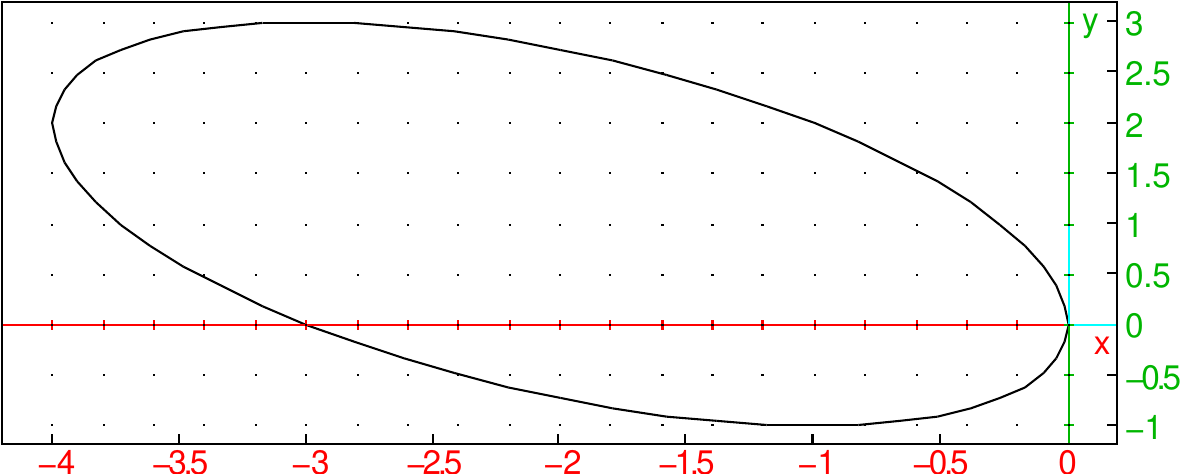
\includegraphics[width=0.75\textwidth]{xcas-conic1.png}
\end{center}
% Output:
% \begin{center}{\tt the graph of the ellipsis of center -2+i and equation 2*x\verb|^|2+2*x*y+2*y\verb|^|2+6*x=0}\end{center}
{\bf Remark}:\\
See also {\tt reduced\_conic} for the parametric equation of the conic.

\subsection{Conic reduction : {\tt reduced\_conic}}\index{reduced\_conic}
\noindent{\tt reduced\_conic} takes two arguments : the equation of a conic
and a vector of variable names.\\ 
{\tt reduced\_conic} returns a list whose elements are:
\begin{itemize}
\item the origin of the conic,
\item the matrix of a basis in which the conic is reduced, 
\item 0 or 1 (0 if the conic is degenerate), 
\item the reduced equation of the conic 
\item a vector of its parametric equations.
\end{itemize}  
Input:
\begin{center}
  {\tt 
    reduced\_conic(2*x\^{}2+2*x*y+2*y\^{}2+5*x+3,[x,y])
  }
\end{center}
Output:
\begin{center}
  {\tt 
  [[-5/3,5/6],[[-1/(sqrt(2)),1/(sqrt(2))],[-1/(sqrt(2)), -1/(sqrt(2))]],1,3*x\verb|^|2+y\verb|^|2+-7/6,[[(-10+5*i)/6+ (1/(sqrt(2))+(i)/(sqrt(2)))*((sqrt(14)*cos(`~t`))/6+ ((i)*sqrt(42)*sin(` t`))/6),` t`,0,2*pi,(2*pi)/60]]]
  }
\end{center}
Which means that the conic is not degenerate, its reduced equation is 
\[3x^2+y^2-7/6=0 \] 
its origin is $-5/3+5*i/6$, its axes are
parallel to the vectors $(-1,1)$ and $(-1,-1)$.
Its parametric equation is
\[ \displaystyle \frac{-10+5*i}{6}+
\frac{(1+i)}{\sqrt 2}*\frac{(\sqrt{14}*cos(t)+i*\sqrt{42}*sin(t))}{6}
\]
where the suggested parameter values for drawing are
$t$ from 0 to $2\pi$ with {\tt tstep}= $2\pi/60$.

{\bf Remark} :\\
Note that if the conic is degenerate and is made of 1 or 2 line(s), 
the lines are not given by 
their parametric equation but by the list of two points of the line.\\ 
Input:
\begin{center}{\tt reduced\_conic(x\verb|^|2-y\verb|^|2+3*x+y+2)}\end{center}
Output:
\begin{center}{\tt [[(-3)/2,1/2],[[1,0],[0,1]],0,x\verb|^;|2-y\verb|^|2, [[(-1+2*i)/(1-i),(1+2*i)/(1-i)], [(-1+2*i)/(1-i),(-1)/(1-i)]]]}\end{center}

\subsection{Graph of a quadric: {\tt quadric}}\index{quadric}
\noindent{\tt quadric} takes as arguments the expression of a
quadric with respect to $x,y,z$. You may also specify the variables
as a vector (second argument) or as second, third and fourth arguments.\\ 
{\tt quadric} draws this quadric.\\
Input:
\begin{center}{\tt 
 quadric(7*x\^{}2+4*y\^{}2+4*z\^{}2+4*x*y- 4*x*z-2*y*z-4*x+5*y+4*z-18)
 }
\end{center}
Output:
\begin{center}
  Ellipsoid of center [0.407407407407,-0.962962962963,-0.537037037037]\\
  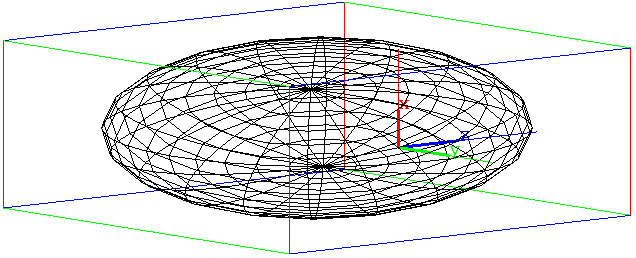
\includegraphics[width=0.75\textwidth]{xcas-quadric1.png}
\end{center}
%\begin{center}{\tt the drawing of the ellipsoid of equation 7*x\verb|^|2+4*y\verb|^|2+4*z\verb|^|2+4*x*y-4*x*z-2*y*z-4*x+5*y+4*z-18=0}\end{center}
See also {\tt reduced\_quadric} for
the parametric equation of the quadric.

\subsection{Quadric reduction : {\tt reduced\_quadric}}\index{reduced\_quadric}
\noindent{\tt reduced\_quadric} takes two arguments : the equation of a 
quadric and a vector of variable names.\\ 
{\tt reduced\_quadric} returns a list whose elements are:
\begin{itemize}
\item the origin, 
\item the matrix of a basis where the quadric is reduced, 
\item 0 or 1 (0 if the quadric is degenerate), 
\item the reduced equation of the quadric 
\item a vector with its parametric equations.
\end{itemize}  
{\bf Warning !} 
{\tt u,v} will be used as parameters of the parametric equations : 
these variables should not be assigned ({\tt purge} them before
calling {\tt reduced\_quadric}).\\
Input :
\begin{center}{\tt reduced\_quadric(7*x\verb|^|2+4*y\verb|^|2+4*z\verb|^|2+ 4*x*y-4*x*z-2*y*z-4*x+5*y+4*z-18)}\end{center}
Output is a list containing :
\begin{itemize}
\item The origin (center of symmetry) of the quadric
\begin{center}{\tt [11/27,(-26)/27,(-29)/54],}\end{center}
\item The matrix of the basis change:
\begin{center}{\tt  [[(sqrt(6))/3,(sqrt(5))/5,(-(sqrt(30)))/15],
    [(sqrt(6))/6,0,(sqrt(30))/6],
    [(-(sqrt(6)))/6,(2*sqrt(5))/5,(sqrt(30))/30]],}\end{center}
\item 1 hence the quadric is not degenerated
\item the reduced equation of the quadric :
\begin{center}{\tt
    0,9*x\verb|^|2+3*y\verb|^|2+3*z\verb|^|2+(-602)/27,}\end{center} 
\item
The parametric equations (in the original frame) are :
\begin{center}{\tt [[(sqrt(6)*sqrt(602/243)*sin(u)*cos(v))/3+
    (sqrt(5)*sqrt(602/81)*sin(u)*sin(v))/5+
    ((-(sqrt(30)))*sqrt(602/81)*cos(u))/15+11/27,
    (sqrt(6)*sqrt(602/243)*sin(u)*cos(v))/6+
    (sqrt(30)*sqrt(602/81)*cos(u))/6+(-26)/27,
    ((-(sqrt(6)))*sqrt(602/243)*sin(u)*cos(v))/6+
    (2*sqrt(5)*sqrt(602/81)*sin(u)*sin(v))/5+
    (sqrt(30)*sqrt(602/81)*cos(u))/30+(-29)/54], 
     u=(0 .. pi),v=(0.. (2*pi)),ustep=(pi/20),
     vstep=((2*pi)/20)]]}\end{center}
\end{itemize}
Hence the quadric is an ellipsoid and its reduced equation is :
\[ 9*x^2+3*y^2+3*z^2+(-602)/27 = 0\]
after the change of origin $[11/27,(-26)/27,(-29)/54]$,
the matrix of basis change {\tt P} is :
\[ \left[
\begin{array}{ccc}
\displaystyle \frac{\sqrt 6}{3} & \displaystyle\frac{\sqrt 5}{5} & \displaystyle-\frac{\sqrt{30}}{15}\\
\displaystyle \frac{\sqrt 6}{6} & 0 & \displaystyle \frac{\sqrt{30}}{6}\\
\displaystyle -\frac{\sqrt 6}{6} & \displaystyle \frac{2\sqrt{5}}{5} & \displaystyle \frac{\sqrt{30}}{30}\\
\end{array}
\right] \]
Its parametric equation is :
\[ \left\{
\begin{array}{l}
x =\displaystyle \frac{\sqrt 6\sqrt{\frac{602}{243}}\sin(u)\cos(v)}{3}+\frac{\sqrt 5\sqrt{\frac{602}{81}}\sin(u)\sin(v)}{5}-\frac{\sqrt{30}\sqrt{\frac{602}{81}}\cos(u)}{15}+\frac{11}{27}\\
y =\displaystyle \frac{\sqrt 6\sqrt{\frac{602}{243}}\sin(u)\cos(v)}{6}+\frac{\sqrt{30}\sqrt{\frac{602}{81}}\cos(u))}{6}-\frac{26}{27}\\
z =\displaystyle \frac{-\sqrt 6\sqrt{\frac{602}{243}}*\sin(u)\cos(v)}{6}+\frac{2\sqrt 5\sqrt{\frac{602}{81}}\sin(u)\sin(v)}{5}+\frac{\sqrt{30}\sqrt{\frac{602}{81}}\cos(u)}{30}-\frac{29}{54}
\end{array}
\right. 
\]
{\bf Remark} :\\
Note that if the quadric is degenerate and made of 1 or 2 plane(s), 
each plane is not given by 
its parametric equation but by the list of a point of the plane
and of a normal vector to the plane.\\ 
Input :
\begin{center}{\tt reduced\_quadric(x\verb|^|2-y\verb|^|2+3*x+y+2)}\end{center}
Output :
\begin{center}{\tt [[(-3)/2,1/2,0],[[1,0,0],[0,1,0],[0,0,-1]],0,x\verb|^|2-y\verb|^|2, [hyperplan([1,1,0],[(-3)/2,1/2,0]), hyperplan([1,-1,0],[(-3)/2,1/2,0])]]}\end{center}

 \section{Multivariate calculus}\label{sec:plusvar}
\subsection{Gradient : {\tt derive deriver diff grad}}\index{derive}\index{diff}\index{grad}\index{deriver}\label{sec:derive}\index{solve}\index{resoudre}
\noindent{\tt derive} (or {\tt diff} or {\tt grad}) takes two arguments : an 
expression $F$ of $n$ real variables and a vector of these variable names.\\
{\tt derive} returns the gradient of $F$,
where the gradient is the vector of all partial derivatives,
for example in dimension $n=3$
\[ \overrightarrow{\mbox{grad}}(F)= [\frac{\partial F}{\partial x},\frac{\partial F}{\partial y},\frac{\partial F}{\partial z}] \]
{\bf Example} \\
Find the gradient of $F(x,y,z)=2x^2y-xz^3$.\\
Input :
\begin{center}{\tt derive(2*x\verb|^|2*y-x*z\verb|^|3,[x,y,z])}\end{center}
or :
\begin{center}{\tt diff(2*x\verb|^|2*y-x*z\verb|^|3,[x,y,z])}\end{center}
or :
\begin{center}{\tt grad(2*x\verb|^|2*y-x*z\verb|^|3,[x,y,z])}\end{center}
Output :
\begin{center}{\tt [2*2*x*y-z\verb|^|3,2*x\verb|^|2,-(x*3*z\verb|^|2)]}\end{center}
Output after simplification with {\tt normal(ans())} :
\begin{center}{\tt [4*x*y-z\verb|^|3,2*x\verb|^|2,-(3*x*z\verb|^|2)]}\end{center}
To find the critical points of 
$F(x,y,z)=2x^2y-xz^3$, input :
\begin{center}{\tt solve(derive(2*x\verb|^|2*y-x*z\verb|^|3,[x,y,z]),[x,y,z])}\end{center} 
Output :
\begin{center}{\tt [[0,y,0]]}\end{center} 

\subsection{Laplacian : {\tt laplacian}}\index{laplacian}
\noindent{\tt laplacian} takes one or two arguments.
\begin{itemize}
\item It can take an integer or floating-point integer $n$.\\
\texttt{laplacian(n)} returns the $n\times n$ discrete Laplacian
matrix; namely the $n \times n$ tridiagonal matrix with 2s on the
main diagonal, $-1$s just above and below the main diagonal.\\
Input :
\begin{center}{\tt laplacian(3)}\end{center}
Output :
\begin{center}{\tt [[2,-1,0],[-1,2,-1],[0,-1,2]]}\end{center}
Input :
\begin{center}{\tt laplacian(2.0)}\end{center}
Output :
\begin{center}{\tt [[2.0,-1.0],[-1.0,2.0]]}\end{center}

\item It can take an 
expression $F$ of $n$ real variables and a vector of these variable names.\\
{\tt laplacian} returns the Laplacian of$F$, that is the sum of all second
partial derivatives, for example in dimension $n=3$:
\[ \nabla^2(F)=\frac{\partial^2 F}{\partial x^2}+\frac{\partial^2 F}{\partial y^2}+\frac{\partial^2 F}{\partial z^2} \]
{\bf Example}\\
Find the Laplacian of $F(x,y,z)=2x^2y-xz^3$.\\
Input :
\begin{center}{\tt laplacian(2*x\verb|^|2*y-x*z\verb|^|3,[x,y,z])}\end{center}
Output :
\begin{center}{\tt 4*y+-6*x*z}\end{center}
\end{itemize}

\subsection{Hessian matrix : {\tt hessian}}\index{hessian}
\noindent{\tt hessian}  takes two arguments : an 
expression $F$ of $n$ real variables and a vector of these variable names.\\
{\tt hessian} returns the hessian matrix of $F$, that is the matrix of the 
derivatives of order 2.\\
{\bf Example}\\
Find the hessian matrix of $F(x,y,z)=2x^2y-xz^3$.\\
Input :
\begin{center}{\tt hessian(2*x\verb|^|2*y-x*z\verb|^|3 , [x,y,z])}\end{center}
Output :
\begin{center}{\tt[[4*y,4*x,-(3*z\verb|^|2)],[2*2*x,0,0],[-(3*z\verb|^|2),0,x*3*2*z]]}\end{center}
To have the hessian matrix at the critical points, first input :
\begin{center}{\tt solve(derive(2*x\verb|^|2*y-x*z\verb|^|3,[x,y,z]),[x,y,z])}\end{center} 
Output is the critical points : 
\begin{center}{\tt [[0,y,0]]}\end{center}
Then, to have the hessian matrix at this points, input : 
\begin{center}{\tt subst([[4*y,4*x,-(3*z\verb|^|2)],[2*2*x,0,0], [-(3*z\verb|^|2),0,6*x*z]],[x,y,z],[0,y,0])}\end{center}
Output :
\begin{center}{\tt [[4*y,4*0,-(3*0\verb|^|2)],[4*0,0,0],[-(3*0\verb|^|2),0,6*0*0]]}\end{center}
and after simplification :
\begin{center}{\tt [[4*y,0,0],[0,0,0],[0,0,0]]}\end{center}

\subsection{Divergence : {\tt divergence}}\index{divergence}
\noindent{\tt divergence} takes two arguments : a vector 
field of dimension $n$ depending on $n$ real variables.\\
{\tt divergence} returns the divergence of $F$ that is the sum 
of the derivative of the $k$-th component with respect
to the $k$-th variable. For example in dimension $n=3$:
\begin{center}
  {\tt divergence([A,B,C],[x,y,z])}=$\displaystyle\frac{\partial A}{\partial x}+\frac{\partial B}{\partial y}+\frac{\partial C}{\partial z}$
\end{center}
Input :
\begin{center}{\tt divergence([x*z,-y\verb|^|2,2*x\verb|^|y],[x,y,z])}\end{center}
Output :
\begin{center}{\tt z+-2*y}\end{center}

\subsection{Rotational : {\tt curl}}\index{curl}
\noindent{\tt curl}  takes two arguments : a 3-d vector field
depending on 3 variables.\\
{\tt curl} returns the rotational of the vector, defined by:
\begin{center}
{\tt curl([A,B,C],[x,y,z])}=$\displaystyle [\frac{\partial C}{\partial y}-\frac{\partial B}{\partial z},\ \frac{\partial A}{\partial z}-\frac{\partial C}{\partial x},\ \frac{\partial B}{\partial x}-\frac{\partial A}{\partial y}]$
\end{center}
Note that $n$ {\bf must be equal to 3}.\\
Input :
\begin{center}{\tt curl([x*z,-y\verb|^|2,2*x\verb|^|y],[x,y,z])}\end{center}
Output :
\begin{center}{\tt [2*x\verb|^|y*log(x),x-2*y*x\verb|^|(y-1),0]}\end{center}

\subsection{Potential : {\tt potential}}\index{potential}
\noindent{\tt potential} takes two arguments : a vector field
$\overrightarrow V$ in $R^n$ with respect to $n$ real variables 
and the vector of these variable names.\\
{\tt  potential} returns, if it is possible, a function $U$ such that 
$\overrightarrow{\mbox{grad}}(U)=\overrightarrow V$. When it is possible, we
say that $\overrightarrow V$ derives the potential $U$, and
$U$ is defined up to a constant.\\
{\tt  potential} is the reciprocal function of {\tt derive}.\\
Input :
\begin{center}{\tt potential([2*x*y+3,x\verb|^|2-4*z,-4*y],[x,y,z])}\end{center}
Output :
\begin{center}{\tt 2*y*x\verb|^|2/
2+3*x+(x\verb|^|2-4*z-2*x\verb|^|2/2)*y}\end{center}
Note that in $\R^3$ 
a vector $\overrightarrow V$ is a gradient if and only if its 
rotational is zero i.e. if {\tt curl(V)=0}.
In time-independent electro-magnetism, 
$\overrightarrow V$=$\overrightarrow E$ is the
electric field and $U$ is the electric potential.

\subsection{Conservative flux field : {\tt vpotential}}\index{vpotential}
\noindent{\tt  vpotential} takes two arguments : a vector field
$\overrightarrow V$ 
in $R^n$ with respect to $n$ real variables 
and the vector of these variable names.\\
{\tt  vpotential} returns, if it is possible, a vector $\overrightarrow U$ such
that $\overrightarrow{\mbox{curl}}(\overrightarrow U)=\overrightarrow V$.
When it is possible we say that  $\overrightarrow V$ is a conservative flux 
field or a solenoidal field.
The general solution is the sum of a particular solution and of the
gradient of an arbitrary function, {\tt Xcas} returns a particular
solution with zero as first component.\\ 
{\tt  vpotential} is the reciprocal function of {\tt curl}.\\
Input :
\begin{center}{\tt vpotential([2*x*y+3,x\verb|^|2-4*z,-2*y*z],[x,y,z]) }\end{center}
Output :~
\begin{center}{\tt [0,(-(2*y))*z*x,-x\verb|^|3/3-(-(4*z))*x+3*y]}\end{center}
In $\R^3$, a vector field $\overrightarrow V$ is a rotational  
if and only if its 
divergence is zero \\({\tt divergence(V,[x,y,z])=0}).
In time-independent electro-magnetism,
$\overrightarrow V$= $\overrightarrow B$ is the magnetic field and
$\overrightarrow U$= $\overrightarrow A$ is the potential vector.

\section{Equations}
\subsection{Define an equation : {\tt equal}}\index{equal}
\noindent{\tt equal} takes as argument the two members of an equation.\\
{\tt equal} returns this equation. It is the prefixed version of {\tt =}\\
Input :
\begin{center}{\tt equal(2x-1,3)}\end{center}
Output :
\begin{center}{\tt (2*x-1)=3}\end{center}
We can also directly write {\tt (2*x-1)=3}.

\subsection{Transform an equation into a difference : {\tt equal2diff}}\index{equal2diff}
\noindent{\tt equal2diff} takes as argument an equation.\\
{\tt equal2diff} returns the difference of the two members of this equation.\\
Input :
\begin{center}{\tt equal2diff(2x-1=3)}\end{center}
Output :
\begin{center}{\tt 2*x-1-3}\end{center}

\subsection{Transform an equation into a list : {\tt equal2list}}\index{equal2list}
\noindent{\tt equal2list} takes as argument an equation.\\
{\tt equal2list} returns the list of the two members of this equation.\\
Input :
\begin{center}{\tt equal2list(2x-1=3)}\end{center}
Output :
\begin{center}{\tt [2*x-1,3]}\end{center}

\subsection{The left member of an equation : {\tt left  gauche lhs}}\index{left|textbf}\index{lhs|textbf}\index{gauche|textbf}
\noindent{\tt left} or {\tt lhs} takes as argument an equation or an 
interval.\\
{\tt left}  or {\tt lhs} returns the left member of this equation or the left
bound  of this interval.\\
Input :
\begin{center}{\tt left(2x-1=3)}\end{center}
Or input:
\begin{center}{\tt lhs(2x-1=3)}\end{center}
Output :
\begin{center}{\tt 2*x-1}\end{center}
Input :
\begin{center}{\tt left(1..3)}\end{center}
Or input:
\begin{center}{\tt lhs(1..3)}\end{center}
Output :
\begin{center}{\tt 1}\end{center}

\subsection{The right member of an equation : {\tt right  droit rhs}}\index{right|textbf}\index{rhs|textbf} \index{droit|textbf}
\noindent{\tt right} or {\tt rhs} takes as argument an equation or an 
interval.\\
{\tt right}  or  {\tt rhs} returns the right member of this equation or the 
right bound of this interval.\\
Input :
\begin{center}{\tt right(2x-1=3)}\end{center}
or :
\begin{center}{\tt rhs(2x-1=3)}\end{center}
Output :
\begin{center}{\tt 3}\end{center}
Input :
\begin{center}{\tt right(1..3)}\end{center}
or :
\begin{center}{\tt rhs(1..3)}\end{center}
Output :
\begin{center}{\tt 3}\end{center}

\subsection{Solving equation(s): {\tt solve}}\index{solve|textbf}
\noindent{\tt solve} solves an equation or a system of polynomial
equations. It takes 2 arguments:
\begin{itemize}
\item Solving an equation\\
{\tt solve} takes as arguments  an equation between two expressions or an 
expression ({\tt =0} is omitted), and a variable name (by default {\tt x}).\\
{\tt solve}  solves this equation.
\item Solving a system of polynomial equations\\
{\tt solve} takes as arguments two vectors : 
a vector of polynomial equations and a 
vector of variable names. \\ 
{\tt solve} solves this polynomial equation system.
\end{itemize}
{\bf Remarks}:
\begin{itemize}
\item In real mode, {\tt solve} returns only real solutions. To have 
the complex solutions, switch to complex mode, e.g. by checking 
{\tt Complex} in the cas configuration, or use the {\tt cSolve}
command.
\item
For trigonometric equations, {\tt solve} returns by default the principal
solutions. To have all the solutions check {\tt All\_trig\_sol} in the cas
configuration.
\end{itemize}
{\bf Examples} :
\begin{itemize}
\item Solve $x^4-1=3$\\
 Input :
\begin{center}{\tt  solve(x\verb|^|4-1=3)}\end{center}
Output in real mode :
\begin{center}{\tt [sqrt(2),-(sqrt(2))]}\end{center}
Output in complex mode :
\begin{center}{\tt [sqrt(2),-(sqrt(2)),(i)*sqrt(2),-((i)*sqrt(2))]}\end{center}
\item Solve $\exp(x)=2$ \\
Input :
\begin{center}{\tt  solve(exp(x)=2)}\end{center}
Output in real mode :
\begin{center}{\tt [log(2)]}\end{center}
\item Find $x,y$ such that $x+y=1,x-y=0$\\
 Input :
\begin{center}{\tt  solve([x+y=1,x-y],[x,y])}\end{center}
Output :
\begin{center}{\tt [[1/2,1/2]] }\end{center}
\item Find $x,y$ such that $x^2+y=2,x+y^2=2$\\
Input :
\begin{center}{\tt  solve([x\verb|^|2+y=2,x+y\verb|^|2=2],[x,y])}\end{center}
Output :
\begin{center}{\tt [[-2,-2],[1,1],[(-sqrt(5)+1)/2,(1+sqrt(5))/2],}\end{center}
\begin{center}{\tt [(sqrt(5)+1)/2,(1-sqrt(5))/2]] }\end{center}
\item Find $x,y,z$ such that $x^2-y^2=0,x^2-z^2=0$\\
Input :
\begin{center}{\tt  solve([x\verb|^|2-y\verb|^|2=0,x\verb|^|2-z\verb|^|2=0],[x,y,z])}\end{center}
Output :
\begin{center}{\tt [[x,x,x],[x,-x,-x],[x,-x,x],[x,x,-x]]}\end{center}
\item Solve $\cos(2*x)=1/2$\\
Input :
\begin{center}{\tt  solve(cos(2*x)=1/2)}\end{center}
Output :
\begin{center}{\tt [pi/6,(-pi)/6]}\end{center}
Output with {\tt All\_trig\_sol} checked :
\begin{center}{\tt [(6*pi*n\_0+pi)/6,(6*pi*n\_0-pi)/6]}\end{center}
\item
Find the intersection of a straight line 
(given by a list of equations) and a plane.\\ For example,
let $D$ be the straight line of cartesian equations 
$[y-z=0,z-x=0]$ and let $P$ the plane of equation $x-1+y+z=0$.
Find the intersection of $D$ and $P$.\\
Input :
\begin{center}{\tt solve([[y-z=0,z-x=0],x-1+y+z=0],[x,y,z])}\end{center}
Output :
\begin{center}{\tt [[1/3,1/3,1/3]]}\end{center}
\end{itemize}

\subsection{Equation solving in $\mathbb C$ : {\tt cSolve}}\index{cSolve}
\noindent{\tt cSolve} takes two arguments and solves an equation or a system
of polynomial equations.
\begin{itemize}
\item solving an equation\\
{\tt cSolve} takes as arguments an equation between two expressions or an 
expression ({\tt =0} is omitted), and a variable name (by default {\tt x}).\\
{\tt cSolve} solves this equation in $\mathbb C$ even if you are in
real mode.
\item solving a system of polynomial equations\\
{\tt cSolve} takes as arguments two vectors : a vector of polynomial equations 
and a vector of variable names. \\
{\tt cSolve} solves this equation system in $\mathbb C$ even if you are in
real mode.
\end{itemize}
Input :
\begin{center}{\tt  cSolve(x\verb|^|4-1=3)}\end{center}
Output :
\begin{center}{\tt [sqrt(2),-(sqrt(2)),(i)*sqrt(2),-((i)*sqrt(2))]}\end{center}
Input :
\begin{center}{\tt  cSolve([-x\verb|^|2+y=2,x\verb|^|2+y],[x,y])}\end{center}
Output :
\begin{center}{\tt [[i,1],[-i,1]]}\end{center}


\section{Linear systems}
In this paragraph, we call the "augmented matrix" of the system
$A \cdot X=B$ (or matrix "representing" the system $A \cdot X=B$),
the matrix obtained by gluing the column vector $B$ or $-B$
to the right of the matrix $A$, as with {\tt border(A,tran(B))}.
   
\subsection{Matrix of a system : {\tt syst2mat}}\index{syst2mat}
\noindent{\tt syst2mat} takes two vectors as arguments. The components of the 
first vector are the equations of a linear system and the components of the
second vector are the variable names.\\
{\tt syst2mat} returns the augmented matrix of the system $AX=B$,
obtained by gluing the column vector $-B$
to the right of the matrix $A$.\\
Input :
\begin{center}{\tt syst2mat([x+y,x-y-2],[x,y])}\end{center}
Output :
\begin{center}{\tt [[1,1,0],[1,-1,-2]]}\end{center}
Input :
\begin{center}{\tt syst2mat([x+y=0,x-y=2],[x,y])}\end{center}
Output :
\begin{center}{\tt [[1,1,0],[1,-1,-2]]}\end{center}
{\bf Warning !!!}\\
The variables (here {\tt x} and {\tt y}) must be purged.

\subsection{Gauss reduction of a matrix : {\tt ref}}\index{ref}\label{ref} \label{sec:ref}
\noindent{\tt ref} is used to solve a linear system of equations written in
matrix form:
 \begin{center}{\tt A*X=B}\end{center}
The argument of {\tt ref} is the augmented matrix of the system
(the matrix obtained by augmenting the matrix {\tt A} to the right with
the column vector {\tt B}).\\
The result is a matrix {\tt [A1,B1]} where {\tt A1} has zeros
under its principal diagonal, and the solutions of:
\begin{center}{\tt A1*X=B1}\end{center} 
are the same as the solutions of:
\begin{center}{\tt A*X=B}\end{center}

For example, solve the system :
\[ \left \{
\begin{array}{lcr} 3x + y & = &-2 \\3x +2y & =& 2 \end{array}\right.
\] 
Input  :
\begin{center}{\tt ref([[3,1,-2],[3,2,2]])}\end{center}
Output :
\begin{center}{\tt [[1,1/3,-2/3],[0,1,4]]}\end{center}
Hence the solution is $y=4$ (last row) and $x=-2$ (substitute $y$ 
in the first row).

\subsection{Gauss-Jordan reduction: {\tt rref gaussjord}}
\index{rref|textbf}
\index{gaussjord|textbf}
\label{sec:rref}

\noindent{\tt rref} solves a linear system of equations written in
matrix form (see also \ref{sec:rrefm}) :
 \begin{center}{\tt A*X=B}\end{center}
{\tt rref} takes one or two arguments.
\begin{itemize}
\item
If {\tt rref}  has only one argument, this argument is the augmented matrix 
of the system (the matrix obtained by augmenting matrix {\tt A} to the 
right with the column vector {\tt B}).\\
The result is a matrix {\tt [A1,B1]} : {\tt A1} has zeros both above and under 
its principal diagonal and has 1 on its principal diagonal, and the solutions 
of:
\begin{center}{\tt A1*X=B1}\end{center} 
are the same as :
\begin{center}{\tt A*X=B}\end{center}
For example, to solve the system:
\[
\left \{
\begin{array}{lcr} 3x + y & = &-2 \\3x +2y & =& 2 \end{array}\right.
\] 
Input :
\begin{center}{\tt rref([[3,1,-2],[3,2,2]])}\end{center}
Output :
\begin{center}{\tt [[1,0,-2],[0,1,4]]}\end{center}
Hence $x=-2$ and $y=4$ is the solution of this system.

\noindent{\tt rref} can also solve several linear systems
of equations having the same first member.
We write the second members as a column matrix.\\ 
Input  :
\begin{center}{\tt rref([[3,1,-2,1],[3,2,2,2]])}\end{center}
Output  :
\begin{center}{\tt [[1,0,-2,0],[0,1,4,1]]}\end{center}
Which means that ($x=-2$ and $y=4$) is the solution of the system
$$\left \{
\begin{array}{lcr} 3x + y & = &-2 \\3x +2y & =& 2 \end{array}\right.$$
and ($x=0$ and $y=1$) is the solution of the system
$$\left \{
\begin{array}{lcr} 3x + y & = &1 \\3x +2y & =& 2 \end{array}\right.$$
\item
If {\tt rref}  has two parameters, the second parameter must be an integer 
$k$, and the Gauss-Jordan reduction will be performed on (at most)
the first $k$ columns.\\
Input  :
\begin{center}{\tt rref([[3,1,-2,1],[3,2,2,2]],1)}\end{center}
Output  :
\begin{center}{\tt [[3,1,-2,1],[0,1,4,1]]}\end{center}
\end{itemize}

\subsection{Solving A*X=B : {\tt simult}}\index{simult}
\noindent{\tt simult} is used to solve a linear system of equations (resp. 
several linear systems of equations with the same matrix {\tt A}) written 
in matrix form (see also \ref{sec:rrefm}) :
\begin{center}{\tt A*X=b  (resp. A*X=B)}\end{center}
{\tt simult} takes as arguments the matrix {\tt A} of the system and the 
column vector (i.e. a one column matrix) {\tt b} of the second 
member of the system (resp.
the matrix {\tt B} whose columns are the 
vectors {\tt b} of the second members of the different systems).\\
The result is a column vector solution of the system (resp. a matrix 
whose columns are the solutions of the different systems).\\
For example, to solve the system :
$$\left \{
\begin{array}{lcr} 3x + y & = &-2 \\3x +2y & =& 2 \end{array}\right.$$ 
Input  :
\begin{center}{\tt simult([[3,1],[3,2]],[[-2],[2]])}\end{center}
Output  :
\begin{center}{\tt [[-2],[4]]}\end{center}
Hence $x=-2$ and $y=4$ is the solution.\\
Input  :
\begin{center}{\tt simult([[3,1],[3,2]],[[-2,1],[2,2]])}\end{center}
Output :
\begin{center}{\tt [[-2,0],[4,1]]}\end{center}
Hence $x=-2$ and $y=4$ is the solution of
$$\left \{
\begin{array}{lcr} 3x + y & = &-2 \\3x +2y & =& 2 \end{array}\right.$$
whereas $x=0$ and $y=1$ is the solution of
$$\left \{
\begin{array}{lcr} 3x + y & = &1 \\3x +2y & =& 2 \end{array}\right.$$

\subsection{Step by step Gauss-Jordan reduction of a matrix : {\tt pivot}}\
index{pivot}
\label{sec:pivot}

\noindent{\tt pivot} takes three arguments : a matrix with $n$ rows and $p$ 
columns and two integers $l$ and $c$ such that $0\leq l<n$, $0\leq c<p$
and $A_{l,c}\neq 0$.\\
{\tt pivot(A,l,c)} performs one step of the Gauss-Jordan method
using {\tt A[l,c]} as pivot and returns an equivalent matrix 
with zeros in the column {\tt c} of {\tt A} (except at row $l$).\\
Input  :
\begin{center}{\tt pivot([[1,2],[3,4],[5,6]],1,1)}\end{center}
Output  :
\begin{center}{\tt [[-2,0],[3,4],[2,0]]}\end{center}
Input  :
\begin{center}{\tt pivot([[1,2],[3,4],[5,6]],0,1)}\end{center}
Output  :
\begin{center}{\tt [[1,2],[2,0],[4,0]]}\end{center}

\subsection{Linear system solving: {\tt linsolve}}\index{linsolve}
\noindent{\tt linsolve} is used to solve a system of linear equations.\\
{\tt linsolve} takes its arguments in two different ways.\\
\begin{itemize}
  \item It can take two arguments, the first is a list of equations or
expressions (in that case the convention is that the equation 
is $expression = 0$), and a list of variable names.\\
{\tt linsolve} returns the solution of the system in a list.\\
Input:
\begin{center}{\tt linsolve([2*x+y+z=1,x+y+2*z=1,x+2*y+z=4],[x,y,z])}\end{center}
Output :
\begin{center}{\tt  [1/-2,5/2,1/-2]}\end{center} 
Which means that
\[ x=-\frac{1}{2}, y=\frac{5}{2}, z=-\frac{1}{2} \]
is the solution of the system :
$$\left\{
\begin{array}{rl}
2x+y+z &=1\\
x+y+2z &=1\\
x+2y+z &=4
\end{array}
\right.$$ 
\item It can take two arguments, the matrix of coefficients of a
system and values of the right hand side in the form of a list.\\
Input:
\begin{center}
  \tt
  linsolve ([[2,1,1], [1,1,2], [1,2,1]], [1,1,4])
\end{center}
Output:
\begin{center}
  \tt
 [-1/2,5/2,-1/2] 
\end{center}
\item
It can take four arguments; the matrices \texttt{P}, \texttt{L},
\texttt{U} from the \texttt{lu} decomposition and the values of the
right hand side in the form of a list.  This is useful when you have
several systems of equations which only differ on their right hand side.\\
Input:
\begin{center}
  \tt
  p,l,u:=lu([[2,1,1],[1,1,2],[1,2,1]])\\
  linsolve(p,l,u,[1,1,4])
\end{center}
Output:
\begin{center}
  \tt
 [-1/2,5/2,-1/2] 
\end{center}
\end{itemize}

If the \texttt{Step by step} option is checked in the general
configuration, a window will also pop up showing:
\begin{verbatim}
 Matrix [[1,1,2, -1], [0,1, -1, -3], [0, -1, -3,1]]
 Row operation L2 <- (1) * L1- (1) * L2
 Matrix [[1,0,3,2], [0,1, -1, -3], [0, -1, -3,1]]
 Row operation L2 <- (1) * L3 - (- 1) * L2
 Matrix [[1,0,3,2], [0,1, -1, -3], [0,0, -4, -2]]
 Reducing column 3 using pivot -4 at row 3
 Matrix [[1,0,3,2], [0,1, -1, -3], [0,0, -4, -2]]
 Row operation L3 <- (-4) * L1- (3) * L3
 Matrix [[-4,0,0, -2], [0,1, -1, -3], [0,0, -4, -2]]
 Row operation L3 <- (-4) * L2 - (- 1) * L3
 End reduction [[-4,0,0, -2], [0, -4,0,10], [0,0, -4, -2]]
\end{verbatim}

The \texttt{linsolve} command also solves systems with coefficients in
$\Z/n\Z$.\\
Input:
\begin{center}
  \tt
  linsolve([2*x+y+z-1,x+y+2*z-1,x+2*y+z-4]\%3,[x,y,z])
\end{center}
Output:
\begin{center}
  \tt
 [1 \% 3,1 \% 3,1 \% 3] 
\end{center}

\subsection{Solving a linear system using the Jacobi iteration method:
\texttt{jacobi\_linsolve}}\index{jacobi\_linsolve}

The \texttt{jacobi\_linsolve} command takes two mandatory arguments
and two optional arguments.  The mandatory arguments are the matrix 
of coefficients of a system and the right hand side of the system as a
list.  The optional arguments are an integer indicating the maximum
number of iterations (by default \texttt{maxiter}) and a positive
number indicating the error tolerance (by default \texttt{epsilon}).\\
\texttt{jacobi\_linsolve} uses the Jacobi iteration method to solve and
return the solution of the system.\\
Input:
\begin{center}
  \tt
  A:=[[100,2],[2,100]];\\
  jacobi\_linsolve(A,[0,1],1e-12);
\end{center}
Output:
\begin{center}
  \tt
 [-0.000200080032,0.0100040016006] 
\end{center}
Input:
\begin{center}
  \tt
  evalf(linsolve(A,[0,1]))
\end{center}
Output:
\begin{center}
  \tt
 [-0.000200080032013,0.0100040016006] 
\end{center}

\subsection{Solving a linear system using the Gauss-Seidel iteration method:
\texttt{gauss\_seidel\_linsolve}}\index{gauss\_seidel\_linsolve}

The \texttt{gauss\_seidel\_linsolve} command takes two mandatory arguments
and two optional arguments.  The mandatory arguments are the matrix 
of coefficients of a system and the right hand side of the system as a
list.  The optional arguments are a positive
number indicating the error tolerance (by default \texttt{epsilon}) and
an integer indicating the maximum number of iterations (by default \texttt{maxiter}).\\
\texttt{jacobi\_linsolve} uses the Gauss-Seidel iteration method to solve and
return the solution of the system.\\
Input:
\begin{center}
  \tt
  A:=[[100,2],[2,100]];\\
  gauss\_seidel\_linsolve(A,[0,1],1e-12);
\end{center}
Output:
\begin{center}
  \tt
[-0.000200080032013,0.0100040016006]
\end{center}

Additionally, \texttt{gauss\_seidel\_linsolve} can take an optional
\emph{first} argument (by default 1) of $\omega$ used for a general
form of the Gauss-Seidel method (the successive overrelaxation
method).\\
Input:
\begin{center}
  \tt
  gauss\_seidel\_linsolve (1.5, A, [0,1], 1e-12);
\end{center}
Output:
\begin{center}
  \tt
 [-0.000200080032218,0.0100040016006]
\end{center}

\subsection{The least squares solution of a linear system:
\texttt{LSQ, lsq}}
\index{LSQ}
\index{lsq}

The \texttt{lsq} (or \texttt{LSQ}) command takes two arguments; a
matrix \texttt{A} and a vector or matrix \texttt{B}.\\
\texttt{lsq} returns the least squares solution to the equation
\texttt{A*X = B}.

\noindent
Input:
\begin{center}
  \tt
  LSQ([[1,2],[3,4]], [5,11])
\end{center}
Output:
\begin{center}
  \tt
 [[1],[2]] 
\end{center}
Input:
\begin{center}
  \tt
  LSQ([[1,2], [3,4]], [[5,7], [11,9]])
\end{center}
Output:
\begin{center}
  \tt
[[1,-5],[2,6]]
\end{center}

Note that\\
Input:
\begin{center}
  \tt
  linsolve([[1,2],[3,4],[3,6]]*[x, y] - [5,11,13],[x, y])
\end{center}
Output:
\begin{center}
  \tt
 [] 
\end{center}
since the linear system has no solution.  We can still find the least
squares solution\\
Input:
\begin{center}
  \tt
  LSQ([[1,2],[3,4],[3,6]],[5,11,13])
\end{center}
Output:
\begin{center}
  \tt
 [[11/5],[11/10]]
\end{center}
The least squares solution\\
Input:
\begin{center}
  \tt
  LSQ ([[3,4]], [12])
\end{center}
Output:
\begin{center}
  \tt
 [[36/25],[48/25]] 
\end{center}
represents the point on the line $3x + 4y = 12$ closest to the origin; \\
Input:
\begin{center}
  \tt
  coordinates(projection(line(3*x+4*y=12),point(0)))
\end{center}
Output:
\begin{center}
  \tt
 [36/25,48/25] 
\end{center}


\subsection{Finding linear recurrences : {\tt reverse\_rsolve}}\index{reverse\_rsolve}
\noindent{\tt reverse\_rsolve} takes as argument a vector 
$v=[v_0...v_{2n-1}]$ made of the first $2n$ terms of a sequence $(v_n)$
which is supposed to verify a linear recurrence relation of 
degree smaller than $n$
\[ x_n*v_{n+k}+...+x_0*v_k=0 \]
where the $x_j$ are $n+1$ unknowns.\\
{\tt reverse\_rsolve} returns the list $x=[x_n,...,x_0]$
of the $x_j$ coefficients (if $x_n\neq 0$ it is reduced to 1).

In other words {\tt reverse\_rsolve} solves the linear system of  
 $n$ equations :
\begin{eqnarray*}
x_n*v_{n}+...+x_0*v_0 &=&0 \\
...\\
x_n*v_{n+k}+...+x_0*v_k &=&0 \\
...\\
x_n*v_{2*n-1}+...+x_0*v_{n-1}&=&0
\end{eqnarray*}
The matrix $A$ of the system has $n$ rows and $n+1$ columns :
\[ A=[[v_0,v_1...v_n],[v_1,v_2,...v_{n-1}],...,[v_{n-1},v_n...v_{2n-1}]] \]
{\tt reverse\_rsolve} returns the list $x=[x_n,...x_1,x_0]$ with $x_n=1$
and $x$ is the solution of the system $A*{\tt revlist}(x)$.

{\bf Examples}
\begin{itemize}
\item Find a sequence satisfying a linear recurrence of degree at 
most 2 whose first elements 1, -1, 3, 3.\\
Input :
\begin{center}{\tt reverse\_rsolve([1,-1,3,3])}\end{center}
Output  :
\begin{center}{\tt  [1,-3,-6]}\end{center} 
Hence $x_0=-6$, $x_1=-3$, $x_2=1$ and the recurrence relation is
 \[ v_{k+2} -3v_{k+1} -6 v_k =0\]
Without {\tt reverse\_rsolve}, we would write the matrix of the system :\\
{\tt [[1,-1,3],[-1,3,3]]} and use the {\tt rref} command :\\
{\tt rref([[1,-1,3],[-1,3,3]])}\\
Output is {\tt [[1,0,6],[0,1,3]]} hence $x_0=-6$ and $x_1=-3$ 
(because $x_2=1$).

\item Find a sequence satisfying a linear recurrence of degree at 
most 3 whose first elements are 1, -1, 3, 3,-1, 1.\\
Input :
\begin{center}{\tt reverse\_rsolve([1,-1,3,3,-1,1])}\end{center}
Output  :
\begin{center}{\tt [1,(-1)/2,1/2,-1]}\end{center} 
Hence so, $x_0=-1$, $x_1=1/2$, $x_2=-1/2$, $x_3=1$, the recurrence
relation is
\[ v_{k+3} -\frac{1}{2} v_{k+2} +\frac{1}{2} v_{k+1} -v_k =0 \]
Without {\tt reverse\_rsolve}, we would write the matrix of the system :\\
{\tt [[1,-1,3,3],[-1,3,3,-1],[3,3,-1,1]]}.\\
Using {\tt rref} command, we would input :\\
{\tt rref([[1,-1,3,3],[-1,3,3,-1],[3,3,-1,1]])}\\
Output is {\tt [1,0,0,1],[0,1,0,1/-2],[0,0,1,1/2]]}
hence $x_0=-1$, $x_1=1/2$ and $x_2=-1/2$ because $x_3=1$),
\end{itemize}

\section{Differential equations}
This section is limited to symbolic (or exact) solutions of
differential equations.
For numeric solutions of differential equations, see {\tt odesolve}.
For graphic representation of solutions of differential equations, 
see  {\tt plotfield}, {\tt plotode} and {\tt interactive\_plotode}. 

\subsection{Solving differential equations : {\tt desolve deSolve 
dsolve}}\index{desolve}\index{deSolve}\index{dsolve}
{\tt desolve} (or {\tt deSolve}) can solve :
\begin{itemize}
\item linear differential equations with constant coefficients,
\item first order linear differential equations,
\item first order differential equations without $y$,
\item first order differential equations without $x$,
\item first order differential equations with separable variables,
\item first order homogeneous differential equations ($y'=F(y/x)$),
\item first order differential equations with integrating factor,
\item first order Bernoulli differential equations ($a(x)y'+b(x)y=c(x)y^n$),
\item first order Clairaut differential equations ($y=x*y'+f(y')$).
\end{itemize}
{\tt desolve} takes as arguments : 
\begin{itemize}
\item  if the independent variable is the current variable (here supposed
to be $x$), 
\begin{itemize}
\item the differential equation (or the list of
the differential equation and of the initial conditions) 
\item the unknown (usually {\tt y}).
\end{itemize}
In the differential equation, the function $y$ is denoted by $y$, 
its first derivative $y \prime$  is denoted by 
${\tt y'}$, and its second derivative $y'{'}$ is written 
${\tt y''}$.\\
For example {\tt desolve(y''+2*y'+y,y)} or \\
{\tt desolve([y''+2*y'+y,y(0)=1,y'(0)=0],y)}.
\item if the independent variable is not the current variable, 
for example $t$ instead of $x$, 
\begin{itemize}
\item the differential equation (or the list of
the differential equation and of the initial conditions), 
\item the variable, e.g. {\tt t} 
\item the unknown as a variable {\tt y} or as a function {\tt y(t)}.
\end{itemize}
In the differential equation, the function $y$ is denoted by $y(t)$,
its derivative $y \prime$  is denoted by
{\tt diff(y(t),t)}, and its second derivative
$y'{'}$  is denoted by {\tt diff(y(t),t\$2)}.\\ 
For example : \\
{\tt desolve(diff(y(t),t\$2)+2*diff(y(t),t)+y(t),y(t))}; or\\
{\tt desolve(diff(y(t),t\$2)+2*diff(y(t),t)+y(t),t,y)};
and \\
\begin{verbatim}
desolve([diff(y(t),t$2)+2*diff(y(t),t)+y(t),
         y(0)=1,y'(0)=0],y(t)); or
desolve([diff(y(t),t$2)+2*diff(y(t),t)+y(t), 
         y(0)=1,y'(0)=0],t,y);
\end{verbatim}
\end{itemize}
If there is no initial conditions (or one initial condition for a second
order equation),
{\tt desolve} returns the general solution in terms of 
constants of integration 
{\tt c\_0, c\_1}, where {\tt y(0)=c\_0} and {\tt y'(0)=c\_1},
or a list of  solutions.\\
{\bf Examples}
\begin{itemize}
\item Examples of second linear differential equations with constant 
coefficients.
\begin{enumerate}
\item 
Solve :
$$y''+y=\cos (x) $$
Input (typing twice prime for {\tt y''}): 
\begin{center}{\tt desolve(y''+y=cos(x),y)}\end{center}
or input :
\begin{center}{\tt desolve((diff(diff(y))+y)=(cos(x)),y)}\end{center}
Output :
\begin{center}{\tt  c\_0*cos(x)+(x+2*c\_1)*sin(x)/2}\end{center}
{\tt c\_0, c\_1} are the constants  of integration : {\tt y(0)=c\_0} and 
{\tt y'(0)=c\_1}.\\ 
If the variable is not {\tt x} but {\tt t}, input : 
\begin{center}
{\tt desolve(derive(derive(y(t),t),t)+y(t)=cos(t),t,y)}
\end{center}
Output :
\begin{center}{\tt  c\_0*cos(t)+(t+2*c\_1)/2*sin(t)}\end{center}
{\tt c\_0, c\_1} are the constants of integration : {\tt y(0)=c\_0} and
{\tt y'(0)=c\_1}.
\item
Solve :
$$y''+y=\cos (x), \; \; y(0)=1 $$
Input :
\begin{center}{\tt desolve([y''+y=cos(x),y(0)=1],y)}\end{center}
Output   :
\begin{center}{\tt [cos(x)+(x+2*c\_1)/2*sin(x)]}\end{center}
the components of this vector are solutions (here there is just one component, 
so we have just one solution depending of the constant {\tt c\_1}).
\item
Solve :
$$y''+y=\cos (x) \; \; (y(0))^2=1 $$
Input :
\begin{center}{\tt desolve([y''+y=cos(x),y(0)\verb|^|2=1],y)}\end{center}
Output :
\begin{center}{\tt [-cos(x)+(x+2*c\_1)/2*sin(x),cos(x)+(x+2*c\_1)/2*sin(x)]}\end{center}
each component of this list is a solution, 
we have two solutions depending
on the constant {\tt c\_1} ($y'(0)=c_1$)
and corresponding to $y(0)=1$ and to $y(0)=-1$.
\item
Solve :
$$y''+y=\cos (x), \; \; (y(0))^2=1 \; \; y'(0)=1$$
Input :
\begin{center}{\tt desolve([y''+y=cos(x),y(0)\verb|^|2=1,y'(0)=1],y)}
\end{center}
Output :
\begin{center}{\tt [-cos(x)+(x+2)/2*sin(x),cos(x)+(x+2)/2*sin(x)]}\end{center}
each component of this list is a solution (we have two solutions).
\item
Solve :
$$y''+2y'+y=0$$
Input :
\begin{center}{\tt desolve(y''+2*y'+y=0,y)}\end{center}
Output :
\begin{center}{\tt (x*c\_0+x*c\_1+c\_0)*exp(-x)}\end{center}
the solution depends of 2 constants of integration : 
{\tt c\_0, c\_1} ({\tt y(0)=c\_0} and {\tt y'(0)=c\_1}).
\item
Solve :
$$y''-6y'+9y=xe^{3x}$$
Input:
\begin{center}{\tt desolve(y''-6*y'+9*y=(x*exp(3*x),y)}\end{center}
Output :
\begin{center}{\tt (x\verb|^|3+(-(18*x))*c\_0+6*x*c\_1+6*c\_0)*1/6*exp(3*x)}\end{center}
the solution depends on 2  constants of integration : 
{\tt c\_0, c\_1} ({\tt y(0)=c\_0} and {\tt y'(0)=c\_1}).
\end{enumerate}
\item Examples of first order linear differential equations.
\begin{enumerate}
\item 
Solve :
$$xy'+y-3x^2=0$$
Input :
\begin{center}{\tt desolve(x*y'+y-3*x\verb|^|2,y)}\end{center}
Output :
\begin{center}{\tt(3*1/3*x\verb|^|3+c\_0)/x }\end{center}
\item
Solve :
$$y'+x*y=0, y(0)=1$$
Input :
\begin{center}{\tt desolve([y'+x*y=0, y(0)=1]),y)}\end{center}
or :
\begin{center}{\tt desolve((y'+x*y=0) \&\& (y(0)=1),y)}\end{center}
Output  :
\begin{center}{\tt [1/(exp(1/2*x\verb|^|2))]}\end{center} 
\item
Solve :
$$x(x^2-1)y'+2y=0$$
Input :
\begin{center}{\tt desolve(x*(x\verb|^|2-1)*y'+2*y=0,y)}\end{center}
Output  :
\begin{center}{\tt (c\_0)/((x\verb|^|2-1)/(x\verb|^|2))}\end{center}
\item
Solve :
$$x(x^2-1)y'+2y=x^2$$
Input :
\begin{center}{\tt desolve(x*(x\verb|^|2-1)*y'+2*y=x\verb|^|2,y)}\end{center}
Output  :
\begin{center}{\tt (ln(x)+c\_0)/((x\verb|^|2-1)/(x\verb|^|2))}\end{center}
\item
If the variable is $t$ instead of $x$, for example  :
$$t(t^2-1)y'(t)+2y(t)=t^2$$
Input :
\begin{center}{\tt desolve(t*(t\verb|^|2-1)*diff(y(t),t)+2*y(t)=(t\verb|^|2),y(t))}\end{center}
Output :
\begin{center}{\tt (ln(t)+c\_0)/((t\verb|^|2-1)/(t\verb|^|2))}\end{center}
\item
Solve :
$$x(x^2-1)y'+2y=x^2,y(2)=0$$
Input :
\begin{center}{\tt desolve([x*(x\verb|^|2-1)*y'+2*y=x\verb|^|2,y(0)=1],y)}\end{center}
Output  :
\begin{center}{\tt [(ln(x)-ln(2))*1/(x\verb|^|2-1)*x\verb|^|2]}\end{center}
\item
Solve :
$$\sqrt{1+x^2}y'-x-y=\sqrt{1+x^2}$$
Input :
\begin{center}{\tt desolve(y'*sqrt(1+x\verb|^|2)-x-y-sqrt(1+x\verb|^|2),y)}\end{center}
Output  :
\begin{center}{\tt (-c\_0+ln(sqrt(x\verb|^|2+1)-x))/(x-sqrt(x\verb|^|2+1))}\end{center}
\end{enumerate}

\item Examples of first differential equations with separable variables.
\begin{enumerate}
\item Solve :
$$y'=2\sqrt{y}$$
Input :
\begin{center}{\tt desolve(y'=2*sqrt(y),y)}\end{center}
Output  :
\begin{center}{\tt [x\verb|^|2+-2*x*c\_0+c\_0\verb|^|2]}\end{center}
\item
Solve :
$$xy'\ln(x)-y(3\ln(x)+1)=0$$
Input :
\begin{center}{\tt desolve(x*y'*ln(x)-(3*ln(x)+1)*y,y)}\end{center}
Output  :
\begin{center}{\tt c\_0*x\verb|^|3*ln(x)}\end{center}
\end{enumerate}

\item Examples of Bernoulli differential equations 
$a(x)y'+b(x)y=c(x)y^n$ where $n$ is a real constant.\\
The method used is to divide the equation by $y^n$, 
so that it becomes a first order linear differential equation 
in $u=1/y^{n-1}$.
\begin{enumerate}
\item 
Solve :
$$xy'+2y+xy^2=0$$
Input :
\begin{center}{\tt desolve(x*y'+2*y+x*y\verb|^|2,y)}\end{center}
Output :
\begin{center}{\tt [1/(exp(2*ln(x))*(-1/x+c\_0))]}\end{center}
\item
Solve :
$$xy'-2y=xy^3$$
Input :
\begin{center}{\tt desolve(x*y'-2*y-x*y\verb|^|3,y)}\end{center}
Output :
\begin{center}{\tt [((-2*1/5*x\verb|^|5+c\_0)*exp(-(4*log(x))))\verb|^|(1/-2),}\end{center}
\begin{center}{\tt -((-2*1/5*x\verb|^|5+c\_0)*exp(-(4*log(x))))\verb|^|(1/-2)]}\end{center}
\item 
Solve :
$$x^2y'-2y=xe^{(4/x)}y^3$$
Input :
\begin{center}{\tt desolve(x*y'-2*y-x*exp(4/x)*y\verb|^|3,y)}\end{center}
Output  :
\begin{center}{\tt [((-2*ln(x)+c\_0)*exp(-(4*(-(1/x)))))\verb|^|(1/-2),}\end{center}
\begin{center}{\tt -(((-2*ln(x)+c\_0)*exp(-(4*(-(1/x)))))\verb|^|(1/-2))]}\end{center}
\end{enumerate}

\item Examples of first order homogeneous differential equations ($y'=F(y/x)$,
the method of integration is to search $t=y/x$ instead of $y$).
\begin{enumerate}
\item 
Solve :
$$3x^3y'=y(3x^2-y^2)$$
Input :
\begin{center}{\tt desolve(3*x\verb|^|3*diff(y)=((3*x\verb|^|2-y\verb|^|2)*y),y)}\end{center}
Output :
\begin{center}{\tt [0,pnt[c\_0*exp((3*1/2)/(` t`\verb|^|2)),` t`*c\_0*exp((3*1/2)/(` t`\verb|^|2))]]}\end{center}
hence the solutions are $y=0$ and the familiy of curves of parametric
equation $x=c_0\exp(3/(2t^2)), y=t*c_0\exp(3/(2t^2))$ 
(the parameter is denoted by {\tt ` t`} in the answer).
\item
Solve :
$$xy'=y+\sqrt{x^2+y^2}$$
Input :
\begin{center}{\tt desolve(x*y'=y+sqrt(x\verb|^|2+y\verb|^|2),y)}\end{center}
Output  :
\begin{center}{\tt [(-i)*x,(i)*x,pnt[c\_0/(sqrt(` t`\verb|^|2+1)-` t`),(` t`*c\_0)/(sqrt(` t`\verb|^|2+1)-` t`)]]}\end{center}
hence the solutions are  :
$$y=ix,y=-ix$$
 and the family of curves of parametric equations
$$x=c_0/(\sqrt{t^2+1}-t), y=t*c_0/(\sqrt{t^2+1}-t)$$ 
(the parameter is denoted by {\tt ` t`} in the answer).
\end{enumerate}


\item Examples of first order differential equations with an 
integrating factor. By multiplying the equation by a function of $x,y$,
it becomes a closed differential form.
\begin{enumerate}
\item 
Solve :
$$yy'+x$$
Input :
\begin{center}{\tt desolve(y*y'+x,y)}\end{center}
Output  :
\begin{center}{\tt [sqrt(-2*c\_0-x\verb|^|2),-(sqrt(-2*c\_0-x\verb|^|2))]}\end{center}
In this example, $xdx+ydy$ is closed, the integrating factor was 1.
\item
Solve :
$$2xyy'+x^2-y^2+a^2=0$$
Input :
\begin{center}{\tt desolve(2*x*y*y'+x\verb|^|2-y\verb|^|2+a\verb|^|2,y)}\end{center}
Output  :
\begin{center}{\tt [sqrt(a\verb|^|2-x\verb|^|2-c\_1*x),-(sqrt(a\verb|^|2-x\verb|^|2-c\_1*x))]}\end{center}
In this example, the integrating factor was $1/x^2$.
\end{enumerate}

\item Example of first order differential equations without $x$.\\
Solve :
$$(y+y')^4+y'+3y=0$$
This kind of equation cannot be solved directly by {\tt Xcas}, we explain
how to solve them with its help. 
The idea is to find a parametric representation of 
$F(u,v)=0$ where the equation is $F(y,y')=0$, 
Let $u=f(t),v=g(t)$ be such a parametrization of $F=0$, then 
$y=f(t)$ and $dy/dx=y'=g(t)$. Hence
\[ dy/dt=f'(t)=y'*dx/dt=g(t)*dx/dt \]
The solution is the curve of parametric equations
$x(t), y(t)=f(t)$, where $x(t)$ is solution of the differential equation 
 $g(t)dx=f'(t)dt$.\\
Back to the example, we put $y+y'=t$, hence:
\[ y=-t-8*t^4, \quad y'=dy/dx=3*t+8*t^4 \quad dy/dt=-1-32*t^3
\] 
therefore
\[ (3*t+8*t^4)*dx=(-1-32*t^3)dt \]
Input :
\begin{center}{\tt desolve((3*t+8*t\verb|^|4)*diff(x(t),t)=(-1-32*t\verb|^|3),x(t))}\end{center}
Output :
\begin{center}{\tt -11*1/9*ln(8*t\verb|^|3+3)+1/-9*ln(t\verb|^|3)+c\_0}\end{center}
eventually the solution is the curve of parametric equation :
\[ x(t)=-11*1/9*\ln(8*t^3+3)+1/-9*\ln(t^3)+c_0,
\quad y(t)=-t-8*t^4 \]

\item Examples of first order 
Clairaut differential equations ($y=x*y'+f(y')$).\\
The solutions are the lines $D_m$ of equation $y=mx+f(m)$ where
 $m$ is a real constant.
\begin{enumerate}
\item Solve :
$$xy'+y'^3-y=0$$
Input :
\begin{center}{\tt desolve(x*y'+y'\verb|^|3-y),y)}\end{center}
Output  :
\begin{center}{\tt c\_0*x+c\_0\verb|^|3}\end{center}
\item 
Solve :
$$y-xy' - \sqrt{a^2+b^2*y'^2}=0$$
Input :
\begin{center}{\tt desolve((y-x*y'-sqrt(a\verb|^|2+b\verb|^|2*y'\verb|^|2),y)}\end{center}
Output  :
\begin{center}{\tt c\_0*x+sqrt(a\verb|^|2+b\verb|^|2*c\_0\verb|^|2)}\end{center}
\end{enumerate}
\end{itemize}

\subsection{Laplace transform and inverse Laplace transform : {\tt
laplace ilaplace invlaplace}}
\index{laplace}
\index{ilaplace}
\index{invlaplace}
\label{sec:lap}

{\tt laplace} and {\tt ilaplace} (or \texttt{invlaplace}) take one, two or three arguments :
 an expression and optionally the name(s) of the variable(s).\\
The expression is  an expression of the current variable (here $x$) or an 
expression of the variable given as second argument.\\
{\tt laplace} returns the Laplace transform of the expression given as argument
and {\tt ilaplace} the inverse Laplace transform of the expression given 
as argument. The result of {\tt laplace} or {\tt ilaplace} is expressed
in terms of the variable given as third argument if supplied
or second argument if supplied or $x$ otherwise.

The Laplace transform ({\tt laplace}) and inverse Laplace transform
({\tt ilaplace}) are useful to solve linear differential equations
with constant coefficients. For example :
$$y \prime \prime +p. y \prime+q. y \ =\ f(x)$$ $$ y(0)=a, \ y\prime(0)=b$$
Denoting by ${\mathcal{L}}$ the Laplace transform,
the following relations hold :
\begin{eqnarray*}
{\mathcal{L}}(y)(x)&=&\int_0^{+\infty}e^{-x u}y(u)du \\
{\mathcal{L}}^{-1}(g)(x)&=&\frac{1}{2i\pi}\int_C e^{z x}g(z)dz
\end{eqnarray*}
where $C$ is a closed contour enclosing the poles of {\tt g}.\\
Input :
\begin{center}{\tt laplace(sin(x))}\end{center}
The expression (here $\sin(x)$) is an expression of the current variable 
(here $x$) and the answer will also be an expression of the current variable 
$x$.\\
Output :
\begin{center}{\tt 1/((-x)\verb|^|2+1)}\end{center}
or :
\begin{center}{\tt laplace(sin(t),t)}\end{center}
here the variable name is $t$ and this name is also used in the answer.\\
Output :
\begin{center}{\tt 1/((-t)\verb|^|2+1)}\end{center}
Or input :
\begin{center}{\tt laplace(sin(t),t,s)}\end{center}
here the variable name is $t$ and the variable name of the answer is $s$.\\
Output:
\begin{center}{\tt 1/((-s)\verb|^|2+1)}\end{center}
The following properties hold :
\begin{eqnarray*}
{\mathcal{L}}(y')(x) &=&-y(0)+x.{\mathcal{L}}(y)(x) \\
{\mathcal{L}}(y'')(x) &=&-y'(0)+x.{\mathcal{L}}(y')(x) \\
 &=& -y'(0)-x.y(0)+x^2.{\mathcal{L}}(y)(x)
\end{eqnarray*}
If $y \prime \prime(x) +p y \prime(x)+q y(x) \ =\ f(x)$, then :
\begin{eqnarray*}
{\mathcal{L}}(f)(x) &=&{\mathcal{L}}(y''+p.y'+q.y)(x) \\
&=& -y'(0)-x y(0)+x^2 {\mathcal{L}}(y)(x)-p y(0)+p x {\mathcal{L}}(y)(x))+q {\mathcal{L}}(y)(x) \\
&=& (x^2+p x+q) {\mathcal{L}}(y)(x)-y'(0)-(x+p) y(0)
\end{eqnarray*}
Therefore, if $a=y(0)$ and $b=y'(0)$, we have
$${\mathcal{L}}(f)(x)=(x^2+p x+q).{\mathcal{L}}(y)(x)-(x+p) a-b$$
and the solution of the differential equation is :
\[ y(x)=
{\mathcal{L}}^{-1}(({\mathcal{L}}(f)(x)+(x+p) a +b)/(x^2+p x+q))
\]
Example :\\
Solve :
\[ y\prime \prime -6 y\prime+9 y \ =\ x e^{3. x},
\quad  y(0)=c\_0, \quad y\prime(0)=c\_1
\]
Here, $p=-6,\ q=9$.\\
Input :
\begin{center}{\tt laplace(x*exp(3*x))}\end{center}
Output :
\begin{center}{\tt 1/(x\verb|^| 2-6*x+9)}\end{center}
Input :
\begin{center}{\tt ilaplace((1/(x\verb|^|2-6*x+9)+(x-6)*c\_0+c\_1)/(x\verb|^|2-6*x+9))}\end{center}
Output :
\begin{center}{\tt (216*x\verb|^|3-3888*x*c\_0+1296*x*c\_1+1296*c\_0)*exp(3*x)/1296}\end{center}
After simplification and factorization ({\tt factor} command) 
the solution $y$ is :
\begin{center}{\tt (-18*c\_0*x+6*c\_0+x\verb|^|3+6*x*c\_1)*exp(3*x)/6}\end{center}
Note that this equation could be solved directly.
Input :
\begin{center}{\tt desolve(y''-6*y'+9*y=x*exp(3*x),y)}\end{center}
Output :
\begin{center}{\tt exp(3*x)*(-18*c\_0*x+6*c\_0+x\verb|^|3+6*x*c\_1)/6}\end{center}

\subsection{Solving linear homogeneous second-order ODE with rational coefficients : {\tt kovacicsols\index{kovacicsols}}}
{\tt kovacicsols} uses Kovacic's algorithm to find a Liouvillian solution of an ordinary linear homogeneous second-order differential equation
\begin{equation}\label{kovacic-ode}a\,y''+b\,y'+c\,y=0,\end{equation}
where $a$, $b$ and $c$ are rational functions of the independent variable. The command takes from one to three arguments :
\begin{itemize}
  \item equation~\eqref{kovacic-ode} as an expression (left-hand side), equality or a list of coefficients~$[a,b,c]$,
  \item independent variable (optional, by default $x$),
  \item dependent variable (optional, by default $y$).
\end{itemize}
The dependent variable should not be specified if the equation~\eqref{kovacic-ode} is entered as a list of coefficients.

The return value can be a list or an expression. An empty list means that there are no Liouvillian solutions to the input equation. If a non-empty list is returned, it contains one or two independent solution(s) $y_1$ (and $y_2$) to the equation~\eqref{kovacic-ode}. The general solution to~\eqref{kovacic-ode} is then
\[ y=C_1\,y_1+C_2\,y_2, \]
where $C_1,C_2\in\mathbb{R}$ are arbitrary constants. However, for some equations only $y_1$ is returned, in which case $y_2$ can be obtained as (using reduction of order) :
\begin{equation}\label{kovacic-reduction}y_2=y_1\,\int y_1^{-2}.\end{equation}
If {\tt kovacicsols} returns an expression, it means that the solution to~\eqref{kovacic-ode} is given implicitly. In that case the return value is a polynomial $P$ of order $n\in\{4,6,12\}$ in the variable {\tt omega\_} (denoted here by $\omega$) with rational coefficients $r_k$, $k=0,1,2,\dots,n$. If $P(\omega_0)=0$ for some $\omega_0$, then $y=\exp\left(\int\omega_0\right)$ is a solution to the equation~\eqref{kovacic-ode}.

\paragraph{Examples.}
In the first example we find the general solution to the equation
\[ y''=\left(\frac{1}{x}-\frac{3}{16\,x^2}\right)\,y. \]
Input :
\begin{center}
  \tt kovacicsols(y\verb|''|=y*(1/x-3/16x\verb|^|2))
\end{center}
Output :
\begin{center}
  \tt [x\verb|^|(1/4)*exp(2*sqrt(x)),x\verb|^|(1/4)*exp(-2*sqrt(x))]
\end{center}
Therefore, $y=C_1\,x^{1/4}\,\mathrm{e}^{2\,\sqrt{x}}+C_2\,x^{1/4}\,\mathrm{e}^{-2\,\sqrt{x}}$ is the general solution.

In the following example we solve the equation
\[ x''(t)+\frac{3\,(t^2-t+1)}{16\,(t-1)^2\,t^2}\,x(t)=0. \]
Input :
\begin{center}
  \tt kovacicsols(x\verb|''|+3*(t\verb|^|2-t+1)/(16*(t-1)\verb|^|2*t\verb|^|2)*x,t,x)
\end{center}
Output :
\begin{center}
  \tt [(-t*(t-1)*(2*t+2*sqrt(t\verb|^|2-t)-1))\verb|^|(1/4), (t*(t-1)*(-2*t+2*sqrt(t\verb|^|2-t)+1))\verb|^|(1/4)]
\end{center}
Now for arbitrary $C_1,C_2\in\mathbb{R}$ we have
\[\begin{split}x(t)=C_1\,\sqrt[4]{t\,(t-1)\,(1-2\,t-2\,\sqrt{t^2-t})}+\\C_2\,\sqrt[4]{t\,(t-1)\,(1-2\,t+2\,\sqrt{t^2-t})}.\end{split}\]

In the next example we find a particular solution to the equation
\[ y''=\frac{4\,x^6-8\,x^5+12\,x^4+4\,x^3+7\,x^2-20\,x+4}{4\,x^4}\,y. \]
Input :
\begin{center}
  \tt r:=(4x\verb|^|6-8x\verb|^|5+12x\verb|^|4+4x\verb|^|3+7x\verb|^|2-20x+4)/(4x\verb|^|4):; kovacicsols(y\verb|''|=r*y)
\end{center}
Output :
\begin{center}
  \tt [(x\verb|^|2-1)/(x*sqrt(x))*exp((x\verb|^|3-2*x\verb|^|2-2)/(2*x))]
\end{center}
Hence $y=(x^2-1)\,x^{-3/2}\,\mathrm{e}^{\frac{x^3-2\,x^2-2}{2\,x}}$ is a solution to the given equation.

A similar output is obtained when solving the equation
\[ y''+y'=\frac{6\,y}{x^2}. \]
Input :
\begin{center}
  \tt kovacicsols(y\verb|''|+y\verb|'|=6y/x\verb|^|2)
\end{center}
Output :
\begin{center}
  \tt [(x\verb|^|2+6*x+12)*exp(-x)/x\verb|^|2]
\end{center}

To solve Titchmarsh equation
\[ y''+(19-x^2)\,y=0, \]
input :
\begin{center}
  \tt kovacicsols(y\verb|''|+(19-x\verb|^|2)*y=0,x,y)
\end{center}
We obtain a particular solution
\[ y=\left(x^9-18\,x^7+\frac{189\,x^5}{2}-\frac{315\,x^3}{2}+\frac{945\,x}{16}\right)\,\exp\left(-\frac{x^2}{2}\right). \]

To find the general solution of Halm's equation
\[ (1+x^2)^2\,y''(x)+3\,y(x)=0, \]
input :
\begin{center}
  \tt sol:=kovacicsols((1+x\verb|^|2)\verb|^|2*y\verb|''|+3y=0,x,y)
\end{center}
Output :
\begin{center}
  \tt [(x\verb|^|2-1)/(sqrt(x\verb|^|2+1))]
\end{center}
The other basic solution is obtained by using~\eqref{kovacic-reduction}. Input :
\begin{center}
  \tt y1:=sol[0]; y2:=normal(y1*int(y1\verb|^|-2,x))
\end{center}
Output :
\begin{center}
  \tt (x\verb|^|2-1)/(sqrt(x\verb|^|2+1)),-x/(sqrt(x\verb|^|2+1))
\end{center}
Therefore, $y=C_1\,\frac{x^2-1}{\sqrt{x^2+1}}+C_2\,\frac{x}{\sqrt{x^2+1}}$, where $C_1,C_2\in\mathbb{R}$.

In the following example we find the general solution of the non-homogeneous equation
\[ y''-\frac{27\,y}{36\,(x-1)^2}=x+4. \]
First we need to find the general solution to the corresponding homogeneous equation $y_h''-\frac{27\,y_h}{36\,(x-1)^2}=0$. Input :
\begin{center}
  \tt sols:=kovacicsols(y\verb|''|-y*27/(36*(x-1)\verb|^|2),x,y)
\end{center}
Output :
\begin{center}
  \tt [(x\verb|^|2-2*x)/(sqrt(x-1))]
\end{center}
We call the obtained solution $y_1$ and find the other basic independent solution by using~\eqref{kovacic-reduction}. Input :
\begin{center}
  \tt y1:=sols[0]:; y2:=y1*int(1/y1\verb|^|2,x)
\end{center}
Output :
\begin{center}
  \tt -1/(sqrt(x-1)*2)
\end{center}
Now the general solution of the homogeneous equation is
\[ y_h=C_1\,y_1+C_2\,y_2=\frac{C_1\,(x^2-2\,x)+C_2}{\sqrt{x-1}},\quad C_1,C_2\in\mathbb{R}. \]
A particular solution $y_p$ of the non-homogeneous equation can be obtained by variation of parameters as
\[ y_p=-y_1\,\int\frac{y_2\,f(x)}{W}\,\mathrm{d}x+y_2\,\int\frac{y_1\,f(x)}{W}\,\mathrm{d}x, \]
where $f(x)=x+4$ and $W$ is the Wronskian of $y_1$ and $y_2$, i.e.~\[W=y_1\,y_2'-y_2\,y_1'\neq 0.\] Input :
\begin{center}
  \tt W:=y1*y2'-y2*y1':; f:=x+4:; yp:=normal(-y1*int(y2*f/W,x)+y2*int(y1*f/W,x))
\end{center}
Output :
\begin{center}
  \tt (4*x\verb|^|3+72*x\verb|^|2-156*x+80)/21
\end{center}
Hence $y_p=\frac{1}{21}\,(4\,x^3+72\,x^2-156\,x+80)$. Now $y=y_p+y_h$. We proceed by checking that it is indeed the general solution of the given equation. Input :
\begin{center}
  \tt purge(C1,C2):; ysol:=yp+C1*y1+C2*y2:; normal(diff(ysol,x,2)-27/(36*(x-1)\verb|^|2)*ysol)==f
\end{center}
Output :
\begin{center}
  \tt true
\end{center}

In the next example we attempt to solve the equation from the original Kovacic's paper :
\[ y''=\left(\frac{3}{16\,x\,(x-1)}-\frac{2}{9\,(x-1)^2}-\frac{3}{16\,x^2}\right)\,y. \]
Input :
\begin{center}
  \tt r:=-3/(16x\verb|^|2)-2/(9*(x-1)\verb|^|2)+3/(16x*(x-1)):; kovacicsols(y\verb|''|=r*y)
\end{center}
Output :
\begin{center}
  \tt -omega\_\verb|^|4*x\verb|^|4*(x-1)\verb|^|4+ omega\_\verb|^|3*x\verb|^|3*(x-1)\verb|^|3*(7*x-3)/3- omega\_\verb|^|2*x\verb|^|2*(x-1)\verb|^|2*(48*x\verb|^|2-41*x+9)/24+ omega\_*x*(x-1)*(320*x\verb|^|3-409*x\verb|^|2+180*x-27)/432+ (-2048*x\verb|^|4+3484*x\verb|^|3-2313*x\verb|^|2+702*x-81)/20736
\end{center}
The solution is $y=\exp\left(\int\omega_0\right)$, where $\omega_0$ is a zero of the above expression, thus being a root of a fourth-order polynomial in $\omega$. In similar cases one can try the Ferrari method to obtain $\omega_0$.

We get similar output while trying to solve the equation
\[ 48\,t\,(t+1)\,(5\,t-4)\,y''+8\,(25\,t+16)\,(t-2)\,y'-(5\,t+68)\,y=0. \]
Input :
\begin{center}
  \tt de:=[48t*(t+1)*(5t-4),8*(25t+16)*(t-2),-(5t+68)]:; kovacicsols(de,t)
\end{center}
Output :
\begin{center}
  \tt omega\_\verb|^|4*(135*t\verb|^|4-616*t\verb|^|3-144*t\verb|^|2+3072*t-4096)/20736- omega\_\verb|^|2*t\verb|^|2*(t+1)*(15*t\verb|^|3-80*t\verb|^|2+80*t+256)/24- t\verb|^|4*(t+1)\verb|^|2*(t+4)*(5*t+4)+ 2*omega\_*t\verb|^|3*(t+1)\verb|^|2*(t-4)*(5*t+8)/3- omega\_\verb|^|3*t*(t+1)*(23*t\verb|^|2-92*t+128)/54
\end{center}

\section{The Z-transform}

\subsection{The Z-transform of a sequence: \texttt{ztrans}}\index{ztrans}

The Z-transform of a sequence $a_0, a_1, \dots, a_n, \dots$ is the
function 
\[ f(z) = \sum_{n=0}^{\infty} \frac{a_n}{z^n}.\]

The \texttt{ztrans} command takes one or three arguments.
\begin{itemize}
  \item A formula in the variable \texttt{x} for the general term
  $a_x$ of a sequence, or
  \item A formula for the general term of a sequence, the variable
  used in the formula, and a variable to be used by the resulting
  function.
\end{itemize}
\texttt{ztrans} returns the Z-transform of the sequence.

For example, the Z-transform of the sequence
\[ 0, 1, 2, 3, \dots\]
is
\[ f(z) = 0 + 1/z + 2/z^2 + 3/z^3 + \dots\]
which has closed form 
\[ f(z) = z/(z-1)^2.\]
\noindent
Input:
\begin{center}
  \tt
  ztrans(x)    
\end{center}
Output:
\begin{center}
  \tt
 x/(x\^{}2-2*x+1) 
\end{center}
Input:
\begin{center}
  \tt
  ztrans(n,n,z)
\end{center}
Output:
\begin{center}
  \tt
 z/(z\^{}2-2*z+1) 
\end{center}

Note that\\
Input:
\begin{center}
  \tt
  ztrans(1)
\end{center}
Output:
\begin{center}
  \tt
 x/(x-1) 
\end{center}
since
\[ \sum_{n=0}^{\infty} 1/x^n = 1/(1-1/x) = x/(x-1).\]
We also have\\
Input:
\begin{center}
  \tt
  ztrans(1,n,z)
\end{center}
Output:
\begin{center}
  \tt
 z/(z-1) 
\end{center}
Note that differentiating both sides of
\[ \sum_{n=0}^{\infty} 1/z^n = z/(z-1)\]
gives us
\[ \sum_{n=0}^{\infty} n/z^{n-1} = 1/(z-1)^2\]
and so, multiplying both sides by $z$,
\[ \sum_{n=0}^{\infty} n/z^{n} = z/(z-1)^2 = z/(z^2 - 2z + 1)\]
as indicated above.


\subsection{The inverse Z-transform of a rational function:
\texttt{invztrans}}\index{invztrans}

The \texttt{invztrans} command takes one or three arguments.
\begin{itemize}
  \item A rational expression in the variable \texttt{x}, or
  \item A rational expression, the variable
  used in the expression, and a variable to be used by the result.
\end{itemize}
\texttt{ztrans} returns the inverse Z-transform, namely a formula for
the general term of a sequence with the given rational expression as
its Z-transform.

Since \texttt{ztrans(1) = x/(x-1)}, we get\\
Input:
\begin{center}
  \tt
  invztrans(x/(x-1))
\end{center}
Output:
\begin{center}
  \tt
 1 
\end{center}
Input:
\begin{center}
  \tt
  invztrans(z/(z-1),z,n)
\end{center}
Output:
\begin{center}
  \tt
 1 
\end{center}

Similarly,\\
Input:
\begin{center}
  \tt
  invztrans(x/(x-1)\^{}2)
\end{center}
Output:
\begin{center}
  \tt
 x 
\end{center}
Input:
\begin{center}
  \tt
  invztrans(z/(z-1)\^{}2,z,n)
\end{center}
Output:
\begin{center}
  \tt
 n 
\end{center}

\section{Other functions}
\subsection{Replace small values by 0: {\tt epsilon2zero}}
\index{epsilon2zero} \label{sec:epsilon2zero}
\noindent{\tt epsilon2zero} takes as argument an expression of {\tt x}.\\
{\tt epsilon2zero} returns the expression where the values of modulus
less than  {\tt epsilon} are replaced by zero. The expression
is not evaluated.\\
The {\tt epsilon}\index{epsilon} value is defined in the {\tt cas} 
configuration (by default {\tt epsilon=1e-10}).\\
Input :
\begin{center}{\tt epsilon2zero(1e-13+x) }\end{center}
Output (with {\tt epsilon=1e-10}) :
\begin{center}{\tt 0+x}\end{center}
Input :
\begin{center}{\tt epsilon2zero((1e-13+x)*100000) }\end{center}
Output (with {\tt epsilon=1e-10}) :
\begin{center}{\tt (0+x)*100000}\end{center}
Input :
\begin{center}{\tt epsilon2zero(0.001+x) }\end{center}
Output (with {\tt epsilon=0.0001}) :
\begin{center}{\tt 0.001+x}\end{center}

\subsection{List of variables : {\tt lname indets}}\index{lname}\index{indets}
\noindent{\tt lname} (or {\tt indets}) takes as argument an expression.\\
{\tt lname} (or {\tt indets}) returns the list of the symbolic
variable names used in this expression.\\
Input :
\begin{center}{\tt lname(x*y*sin(x))}\end{center}
Output :
\begin{center}{\tt  [x,y]}\end{center}
Input :
\begin{center}{\tt a:=2;assume(b>0);assume(c=3);}\end{center}
\begin{center}{\tt lname(a*x\verb|^|2+b*x+c)}\end{center}
Output :
\begin{center}{\tt  [x,b,c]}\end{center}

\subsection{List of variables and of expressions : {\tt lvar}}\index{lvar}\label{sec:lvar}
\noindent{\tt lvar} takes as argument an expression.\\
{\tt lvar}  returns a list of variable names and non-rational
expressions such that its argument is a rational fraction
with respect to the variables and expressions of the list.\\
Input :
\begin{center}{\tt lvar(x*y*sin(x)\verb|^|2)}\end{center}
Output :
\begin{center}{\tt [x,y,sin(x)]}\end{center}
Input :
\begin{center}{\tt lvar(x*y*sin(x)\verb|^|2+ln(x)*cos(y))}\end{center}
Output :
\begin{center}{\tt [x,y,sin(x),ln(x),cos(y)]}\end{center}
Input :
\begin{center}{\tt lvar(y+x*sqrt(z)+y*sin(x))}\end{center}
Output :
\begin{center}{\tt [x,y,sqrt(z),sin(x)]}\end{center}

\subsection{List of variables of an algebraic expressions: {\tt algvar}}\index{algvar}
\noindent{\tt algvar} takes as argument an expression.\\ 
{\tt algvar} returns the list of the symbolic
variable names used in this expression. The list is ordered
by the algebraic extensions required to build the original expression.\\
Input :
\begin{center}{\tt algvar(y+x*sqrt(z))}\end{center}
Output :
\begin{center}{\tt  [[y,x],[z]]}\end{center}
Input :
\begin{center}{\tt algvar(y*sqrt(x)*sqrt(z))}\end{center}
Output :
\begin{center}{\tt  [[y],[z],[x]]}\end{center}
Input :
\begin{center}{\tt algvar(y*sqrt(x*z))}\end{center}
Output :
\begin{center}{\tt  [[y],[x,z]]}\end{center}
Input :
\begin{center}{\tt algvar(y+x*sqrt(z)+y*sin(x))}\end{center}
Output :
\begin{center}{\tt [[x,y,sin(x)],[z]]}\end{center}

\subsection{Test if a variable is in an expression : {\tt has}}\index{has|textbf}
\noindent{\tt has} takes as argument an expression and the name of a 
variable.\\
{\tt has} returns {\tt 1} if this variable is in this expression, and else 
returns {\tt 0}.\\
Input :
\begin{center}{\tt has(x*y*sin(x),y)}\end{center}
Output :
\begin{center}{\tt  1}\end{center}
Input :
\begin{center}{\tt has(x*y*sin(x),z)}\end{center}
Output :
\begin{center}{\tt  0}\end{center}

\subsection{Numeric evaluation : {\tt evalf}}\index{evalf}
\noindent{\tt evalf} takes as argument an expression or a matrix.\\
{\tt evalf} returns the numeric value of this expression or of this matrix.\\
Input :
\begin{center}{\tt evalf(sqrt(2))}\end{center} 
Output :
\begin{center}{\tt 1.41421356237}\end{center}
Input :
\begin{center}{\tt evalf([[1,sqrt(2)],[0,1]])}\end{center} 
Output :
\begin{center}{\tt [[1.0,1.41421356237],[0.0,1.0]]}\end{center}

\subsection{Rational approximation : {\tt float2rational exact}}\index{float2rational}\index{exact}
\noindent{\tt float2rational} (or {\tt exact}) 
takes as argument an expression.\\
{\tt float2rational} returns a rational approximation of 
all the floating point numbers $r$ contained in this expression, such
that $|r-\mbox{\tt float2rational}(r)|<\epsilon$, where
$\epsilon$  is defined by {\tt epsilon} in the {\tt cas} configuration 
({\tt Cfg} menu, or {\tt cas\_setup} command).\\
Input :
\begin{center}{\tt float2rational(1.5)}\end{center}
Output :
\begin{center}{\tt 3/2}\end{center}
Input :
\begin{center}{\tt float2rational(1.414)}\end{center}
Output :
\begin{center}{\tt 707/500}\end{center}
Input :
\begin{center}{\tt float2rational(0.156381102937*2)}\end{center}
Output :
\begin{center}{\tt 5144/16447}\end{center}
Input :
\begin{center}{\tt float2rational(1.41421356237)}\end{center}
Output :
\begin{center}{\tt 114243/80782}\end{center}
Input :
\begin{center}{\tt float2rational(1.41421356237\verb|^|2)}\end{center}
Output :
\begin{center}{\tt 2}\end{center}

\section{The day of the week: \texttt{dayofweek}}\index{dayofweek}

The \texttt{dayofweek} command takes as arguments three integers; the
first represents the day of the month, the second the month, and the
third the year.  The resulting date should be after 15 October 1582.\\
\texttt{dayofweek} returns an integer from 0 to 6; 0 represents a
Sunday, 1 represents Monday, etc.\\
Input:
\begin{center}
  \tt
  dayofweek(15,10,1582)
\end{center}
Output:
\begin{center}
  \tt
 5 
\end{center}
This indicates that 15 October 1582 was on a Friday.

The Gregorian calendar, the calendar used by most of the world, was
introduced on 15 October 1582.  Before that, the Julian calendar was
used, which had a leap year every four years and so used years with an
average of 365.25, which is slightly off from the actual value of
about 365.242 days.  To deal with this, the Gregorian calendar was
introduced, which kept years for every year divisible by 4, except if
a year is divisible by 100 but not 400 it is not a leap year.  This
gives an average length of year that is accurate to within 1 day every
3000 years.

Many countries switched from the Julian calendar to the Gregorian
calendar after 4 October 1582 in the Julian calendar, and the next day
was 15 October 1582.

\noindent
Input:
\begin{center}
  \tt
  dayofweek(1,10,2014)
\end{center}
Output:
\begin{center}
  \tt
 3 
\end{center}
This means that 1 October, 2014 was a Wednesday.

\chapter{Metric properties of curves}

\section{The center of curvature}

Let $\Gamma$ be a curve in space parameterized by a
continuously differentiable function, and $M_0$ be a point on the
curve.  The curve will have an arclength parameterization; namely, it
can be parameterized by a function $M(s)$, where $M(0) = M_0$ and $|s|$
is the length of the curve from $M_0$ to $M(s)$, in the direction of
the curve if $s>0$ and the opposite direction if $s<0$.

For such a $\Gamma$, the vector $T(s) = M'(s)$ will be the unit tangent
to the curve at $M(s)$, and $N(s) = T'(s)$ will be perpendicular to
the tangent.  The circle through $M(s)$ with center at $M(s) + N(s)$
is called the \emph{osculating circle} to $\Gamma$ at $M(s)$.
Informally, the osculating circle is the circle through $M(s)$ which
most closely approximates $\Gamma$.  The set of all centers of
curvature is another curve, called the \emph{evolute} of $\Gamma$.

The radius of the osculating circle is $|N(s)|$ and is called the
\emph{radius of curvature} of $\Gamma$ at $M(s)$.  The reciprocal of
this is called the \emph{curvature} of $\Gamma$ at $M(s)$.  

\section{Computing the curvature and related values:
\texttt{curvature, osculating\_circle,
evolute}}\index{curvature}\index{osculating\_circle}\index{evolute}

The \texttt{curvature} command takes two arguments and an optional
third argument.  The first
argument is a curve, and the second argument is a point on the curve.
If the curve is given by a parameterization, the second argument is the 
parameter, and an optional third argument is a value of the parameter.\\
\texttt{curvature} returns the curvature of the curve at
the given point.\\
Input:
\begin{center}
  \tt
  curvature(plot(x\^{}2),point(1,1))
\end{center}
Output:
\begin{center}
  \tt
 2/25*sqrt(5) 
\end{center}
Input:
\begin{center}
  \tt
  trigsimplify(curvature([5*cos(t),5*sin(t)],t))
\end{center}
Output:
\begin{center}
  \tt
 1/5
\end{center}
Input:
\begin{center}
  \tt
  curvature([2*cos(t),3*sin(t)],t,pi/2)
\end{center}
Output:
\begin{center}
  \tt
 3/4 
\end{center}

The \texttt{osculating\_circle} command takes two or three arguments.
The arguments can be either a curve in the plane and a point on the
curve, or the parameterization of a curve in the plane, the parameter,
and a value of the parameter.\\
\texttt{osculating\_circle} returns and draws the osculating circle.\\
Input:
\begin{center}
  \tt
  osculating\_circle(plot(x\^{}2),point(1,1))
\end{center}
Output:
\begin{center}
  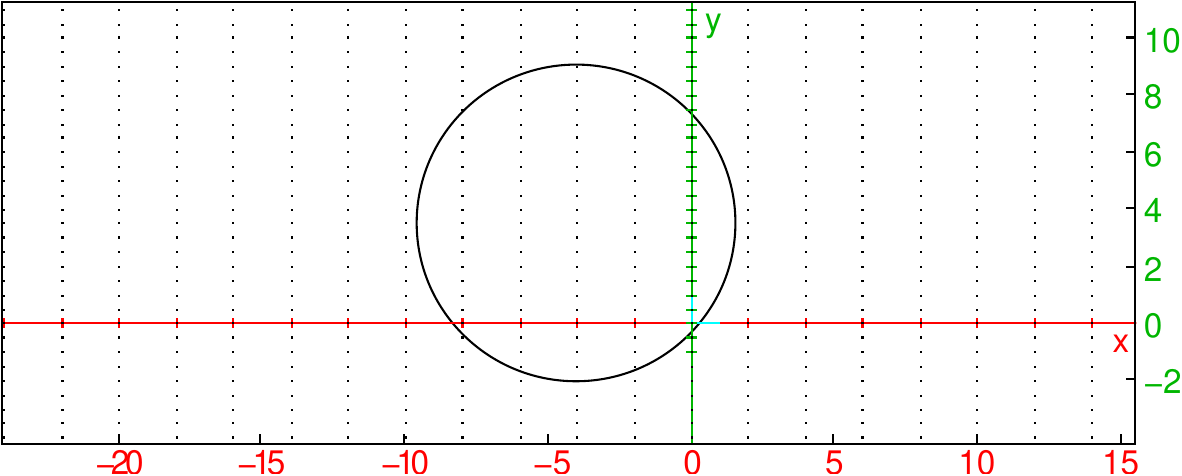
\includegraphics[width=0.75\textwidth]{xcas-osculatingcircle.png}
\end{center}
Input:
\begin{center}
  \tt
  equation(osculating\_circle(plot(x\^{}2),point(1,1)))
\end{center}
Output:
\begin{center}
  \tt
 (x+4)\^{}2+(y-7/2)\^{}2=(125/4) 
\end{center}
Input:
\begin{center}
  \tt
  equation(osculating\_circle([t\^{}2,t\^{}3],t,1))
\end{center}
Output:
\begin{center}
  \tt
 (x+11/2)\^{}2+(y-16/3)\^{}2=(2197/36) 
\end{center}

The \texttt{evolute} command takes one or two arguments.
The arguments can be either a curve in the plane, or 
the parameterization of a curve in the plane and the parameter.\\
\texttt{evolute} draws and returns the evolute of the curve.\\
Input:
\begin{center}
  \tt
  evolute(plot(x\^{}2))
\end{center}
Output:
\begin{center}
  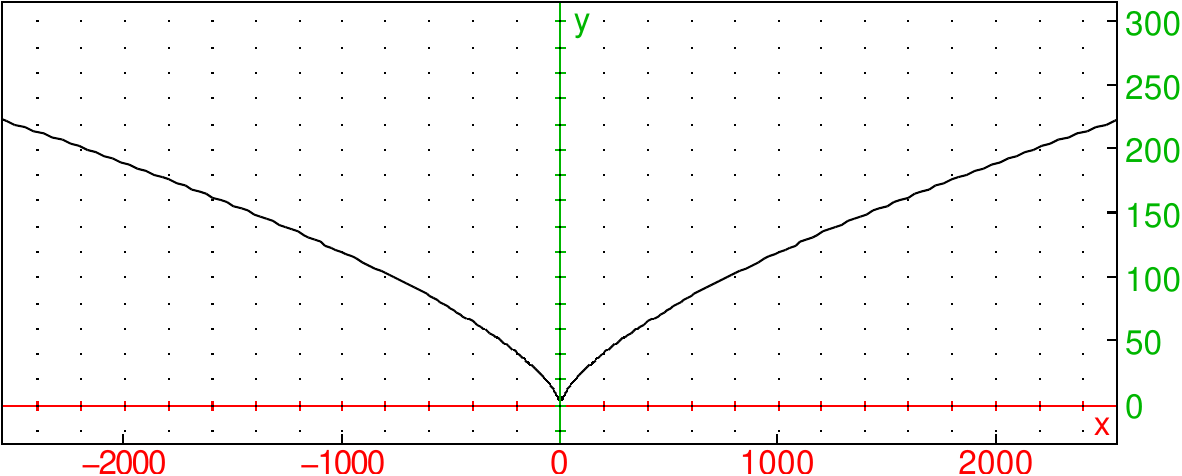
\includegraphics[width=0.75\textwidth]{xcas-evolute.png}
\end{center}
Input:
\begin{center}
  \tt
  equation(evolute(plot(x\^{}2)))
\end{center}
Output:
\begin{center}
  \tt
 27*x\^{}2-16*y\^{}3+24*y\^{}2-12*y+2=0 
\end{center}
Input:
\begin{center}
  \tt
  equation(evolute([t\^{}2,t],t))
\end{center}
Output:
\begin{center}
  \tt
 16*x\^{}3-24*x\^{}2+12*x-27*y\^{}2-2=0 
\end{center}

\chapter{Graphs}\label{sec:plot}

\section{Generalities}

Most graph instructions take expressions as arguments. A few
exceptions (mostly Maple-compatibility instructions) also accept
functions. 
Some optional arguments, like {\tt color, thickness}, can  be used as optional
attributes in all graphic instructions. They are described below.

If a graph depends on a user-defined function, you may want to define
the function when the parameter is a formal variable.  For this, it
can be useful to test the type of the parameter while the function is
being defined.

For example, suppose \texttt{f} and \texttt{g} are defined by\\
\begin{verbatim}
f(x):= {
  if (type(x)!=DOM_FLOAT) return 'f'(x); 
  while(x>0){ x--; } 
  return x; 
}
\end{verbatim}
and
\begin{verbatim}
g(x):= {
  while(x>0){ x--; } 
  return x; 
}:;
\end{verbatim}
Graphing these, with\\
Input:
\begin{center}
  \tt
  F := plotfunc(f(x))
\end{center}
Input:
\begin{center}
  \tt
  G := plotfunc(g(x))
\end{center}
will both produce the same graph.  However, here the graphic
\texttt{G} won't be reusable.  Entering\\
Input:
\begin{center}            
  \tt
  F
\end{center}
reproduces the graph, but entering\\
Input:
\begin{center}
  \tt
  G
\end{center}
produces the error\\
Output:
\begin{center}
  \tt
  "Unable to eval test in loop : x>0.0 Error: Bad Argument Value Error:
  Bad Argument Value"
\end{center}
Internally, \texttt{F} and \texttt{G} contain the formal expressions
\texttt{f(x)} and \texttt{g(x)}, respectively.  When \texttt{Xcas}
tries to evaluate \texttt{F} and \texttt{G},  \texttt{x} has no value
and so the test \texttt{x > 0} produces an error in \texttt{g(x)}, but
the line \verb|if (type(x)!=DOM_FLOAT) return 'f'(x);| avoids this
problem in \texttt{f(x)}.

\section{The graphic screen}

A graphic screen, either two- or three-dimensional as appropriate,
automatically opens in response to a graphic command.  
Alternatively, a graphic screen with its own command line will open
with keystrokes; \texttt{Alt-g} for a two-dimensional screen and
\texttt{Alt-h} for a three-dimensional screen.
The graphic screen will have an array of buttons at the top right.
\begin{itemize}
  \item There will be red arrows for moving the image in the $x$ direction.
  \item There will be green arrows for moving the image in the $y$
  direction.
  \item There will be blue arrows for zooming in and out in a
  two-dimensional screen, and moving the image in the $z$ direction in
  a three-dimensional screen.
  \item There will be \texttt{in} and \texttt{out} buttons for zooming
  in and out.
  \item There will be a \texttt{\_|\_} button to orthonormalize the
  graphic.
  \item There will be a \texttt{$\blacktriangleright$|} button to
  start and stop animations.
  \item There will be an \texttt{auto} button to do automatic scaling.
  \item There will be a \texttt{cfg} button which will bring up a
  configuration screen (see XXXX).
  \item There will be an \texttt{M} button which is a menu.  The menu
  has submenus:
  \begin{itemize}
    \item \texttt{View} which has entries which do the same as the
    buttons.
    \item \texttt{Trace} for working with traces.
    \item \texttt{Animation} for working with animations.
    \item \texttt{3-d} for working with three-dimensional graphics.
    \item \texttt{Export/Print} to export and print the graphic.
  \end{itemize}
\end{itemize}

The image can also be moved in the screen by clicking and dragging with the
mouse.  Scrolling with the mouse will also zoom the images.

\section{Graph and geometric objects attributes}
There are two kinds of attributes: global attributes of a graphic
scene and individual attributes. 

\subsection{Individual attributes}
\index{color@{\it color}|textbf}
\index{display@{\it display}|textbf}
\index{black@\texttt{black}}
\index{white@\texttt{white}}
\index{red@\texttt{red}}
\index{blue@\texttt{blue}}
\index{green@\texttt{green}}
\index{magenta@\texttt{magenta}}
\index{cyan@\texttt{cyan}}
\index{yellow@\texttt{yellow}}
\index{rhombus\_point@\texttt{rhombus\_point}}
\index{plus\_point@\texttt{plus\_point}}
\index{square\_point@\texttt{square\_point}}
\index{cross\_point@\texttt{cross\_point}}
\index{triangle\_point@\texttt{triangle\_point}}
\index{star\_point@\texttt{star\_point}}
\index{point\_point@\texttt{point\_point}}
\index{invisible\_point@\texttt{invisible\_point}}
\index{point\_width\_1@\texttt{point\_width\_1}}
\index{point\_width\_2@\texttt{point\_width\_2}}
\index{point\_width\_3@\texttt{point\_width\_3}}
\index{point\_width\_4@\texttt{point\_width\_4}}
\index{point\_width\_5@\texttt{point\_width\_5}}
\index{point\_width\_6@\texttt{point\_width\_6}}
\index{point\_width\_7@\texttt{point\_width\_7}}
\index{line\_width\_1@\texttt{line\_width\_1}}
\index{line\_width\_2@\texttt{line\_width\_2}}
\index{line\_width\_3@\texttt{line\_width\_3}}
\index{line\_width\_4@\texttt{line\_width\_4}}
\index{line\_width\_5@\texttt{line\_width\_5}}
\index{line\_width\_6@\texttt{line\_width\_6}}
\index{line\_width\_7@\texttt{line\_width\_7}}
\index{dash\_line@\texttt{dash\_line}}
\index{solid\_line@\texttt{solid\_line}}
\index{dashdot\_line@\texttt{dashdot\_line}}
\index{dashdotdot\_line@\texttt{dashdotdot\_line}}
\index{cap\_flat\_line @\texttt{cap\_flat\_line }}
\index{cap\_square\_line@\texttt{cap\_square\_line}}
\index{cap\_round\_line@\texttt{cap\_round\_line}}
\index{quandrant1@\texttt{quandrant1}}
\index{quandrant2@\texttt{quandrant2}}
\index{quandrant3@\texttt{quandrant3}}
\index{quandrant4@\texttt{quandrant4}}
\index{hidden\_name@\texttt{hidden\_name}}
\index{filled@\texttt{filled}}
\index{gl\_texture@\texttt{gl\_texture}}
\index{gl\_material@\texttt{gl\_material}}


Graphic attributes are optional arguments of the
form {\tt display=value}, they must be given
as the last argument of a graphic instruction. Attributes
are ordered in several categories: color, point shape, point width,
line style, line thickness, legend value, position and presence. 
In addition, surfaces may be filled or not, 3-d surfaces
may be filled with a texture, 3-d objects may also have properties
with respect to the light. 
Attributes of different categories
may be added, e.g. \\
{\tt plotfunc($x^2+y^2$,[x,y],display=red+line\_width\_3+filled)}
\begin{itemize}
\item Colors {\tt display=} or {\tt color=}
\begin{itemize}
\item {\tt black}, {\tt white}, {\tt red}, {\tt blue}, {\tt green}, 
{\tt magenta}, {\tt cyan}, {\tt yellow},
\item a numeric value between 0 and 255,
\item a numeric value between 256 and 256+7*16+14 for a color of the
rainbow,
\item any other numeric value smaller than 65535, the rendering
is not guaranteed to be portable.
\end{itemize}
\item Point shapes {\tt display=} one of the following value
{\tt rhombus\_point plus\_point  square\_point cross\_point 
triangle\_point star\_point point\_point invisible\_point}
\item Point width: {\tt display=} one of the following value
{\tt point\_width\_n} where {\tt n} is an
integer between 1 and 7
\item Line thickness: {\tt thickness=n}
or {\tt display=line\_width\_n} where {\tt n} is an
integer between 1 and 7 or 
\item Line shape: {\tt display=} one of the following values
{\tt dash\_line solid\_line dashdot\_line dashdotdot\_line
  cap\_flat\_line cap\_square\_line cap\_round\_line }
\item Legend, value: {\tt legend="legendname"};
 position: {\tt display=} one of
{\tt quandrant1 quadrant2 quadrant3 quadrant4}
corresponding to the position of the legend of the object 
(using the trigonometric plane conventions).
The legend is not displayed if the attribute 
{\tt display=hidden\_name} is added
\item {\tt display=filled} specifies that surfaces will be filled,
\item {\tt gl\_texture="picture\_filename"} is used to fill 
a surface with a texture.  
Cf. the interface manual for a more complete
description and for {\tt gl\_material=} options.
\end{itemize}
{\bf Examples}\\
Input :
\begin{center}{\tt polygon(-1,-i,1,2*i,legend="P")}\end{center}
Input :
\begin{center}{\tt point(1+i,legend="hello")}\end{center}
Input :
\begin{center}{\tt A:=point(1+i);B:=point(-1);display(D:=droite(A,B),hidden\_name)}\end{center}
Input :
\begin{center}{\tt color(segment(0,1+i),red)}\end{center}
Input :
\begin{center}{\tt segment(0,1+i,color=red)}\end{center}

\subsection{Global attributes}
\index{title@\textit{title}}
\index{labels@\textit{labels}}
\index{gl\_x\_axis\_name@\textit{gl\_x\_axis\_name}}
\index{gl\_y\_axis\_name@\textit{gl\_y\_axis\_name}}
\index{gl\_z\_axis\_name@\textit{gl\_z\_axis\_name}}
\index{gl\_x\_axis\_unit@\textit{gl\_x\_axis\_unit}}
\index{gl\_y\_axis\_unit@\textit{gl\_y\_axis\_unit}}
\index{gl\_z\_axis\_unit@\textit{gl\_z\_axis\_unit}}
\index{legend@\textit{legend}}
\index{axes@\textit{axes}}
\index{gl\_texture@\textit{gl\_texture}}
\index{gl\_x@\textit{gl\_x}}
\index{gl\_y@\textit{gl\_y}}
\index{gl\_z@\textit{gl\_z}}
\index{gl\_x\_tick@\textit{gl\_x\_tick}}
\index{gl\_y\_tick@\textit{gl\_y\_tick}}
\index{gl\_z\_tick@\textit{gl\_z\_tick}}
\index{gl\_shownames@\textit{gl\_shownames}}
\index{gl\_rotation@\textit{gl\_rotation}}
\index{gl\_quaternion@\textit{gl\_quaternion}}

These attributes are shared by all objects of the same scene
\begin{itemize}
\item {\tt title="titlename"} defines the title
\item {\tt labels=["xname","yname","zname"]}: names of the $x,y,z$
axis
\item {\tt gl\_x\_axis\_name="xname"}, {\tt gl\_y\_axis\_name="yname"},
{\tt gl\_z\_axis\_name=""}: individual definitions
of the names of the $x,y,z$ axis
\item {\tt legend=["xunit","yunit","zunit"]}: units for the
$x,y,z$ axis
\item {\tt gl\_x\_axis\_unit="xunit"}, {\tt  gl\_y\_axis\_unit="yunit"},
{\tt gl\_z\_axis\_unit=""}: individual definition
of the units of the $x,y,z$ axis
\item {\tt axes=true or false} show or hide axis
\item {\tt gl\_texture="filename"}: background image
\item {\tt gl\_x=xmin..xmax}, {\tt gl\_y=ymin..ymax},
{\tt gl\_z=zmin..zmax}: set the graphic configuration 
(do not use for interactive scenes)
\item {\tt gl\_xtick=}, {\tt gl\_ytick=}, {\tt gl\_ztick=}:
set the tick mark for the axis 
\item {\tt gl\_shownames=true or false}: show or hide objects names
\item {\tt gl\_rotation=[x,y,z]}: defines the rotation axis
for the animation rotation of 3-d scenes.
\item {\tt gl\_quaternion=[x,y,z,t]}: defines the quaternion
for the visualization in 3-d scenes (do not use for interactive
scenes)
\item a few other OpenGL light configuration options are
available but not described here.
\end{itemize}
{\bf Examples}\\
Input :
\begin{center}{\tt legend=["mn","kg"]}\end{center}
Input :
\begin{center}{\tt title="median\_line";triangle(-1-i,1,1+i);median\_line(-1-i,1,1+i);median\_line(1,-1-i,1+i);median\_line(1+i,1,-1-i)}\end{center}
Input :
\begin{center}{\tt labels=["u","v"];plotfunc(u+1,u)}\end{center}

\section{Graph of a function : {\tt plotfunc funcplot DrawFunc Graph}}\index{plotfunc|textbf}\index{funcplot|textbf}\index{DrawFunc|textbf}\index{Graph|textbf}\index{xstep@{\sl xstep}}\index{ystep@{\sl ystep}}\index{zstep@{\sl zstep}}\index{nstep@{\sl nstep}}

\subsection{2-d graph}\label{sec:plotfunc}
\noindent{\tt plotfunc(f(x),x)} draws the graph of $y=f(x)$ for $x$ in
the default interval, 
{\tt plotfunc(f(x),x=a..b)} draws the graph of $y=f(x)$ for $a\leq x\leq b$.
{\tt plotfunc} accepts an optional \verb|xstep=...| argument to 
specify the discretization step in $x$.\\
Input :
\begin{center}{\tt  plotfunc(x\verb|^|2-2)}\end{center}
or :
\begin{center}{\tt  plotfunc(a\verb|^|2-2,a=-1..2)}\end{center}
Output :
\begin{center}{\tt the graph of y=x\verb|^|2-2}\end{center}
Input :
\begin{center}{\tt  plotfunc(x\verb|^|2-2,x,xstep=1)}\end{center}
Output :
\begin{center}{\tt a polygonal line which is a bad representation of y=x\verb|^|2-2 }\end{center}
It is also possible to specify the number of points used for the 
representation of the function with \verb|nstep=| instead of \verb|xstep=|.
For example, input~:
\begin{center}{\tt  plotfunc(x\verb|^|2-2,x=-2..3,nstep=30)}\end{center}

\subsection{3-d graph}\label{sec:plotfunc3}
\noindent{\tt plotfunc} takes two main arguments : an expression of two 
variables or a list of several expressions of two variables and the list of 
these two variables, where each variable may be replaced by
an equality variable=interval to specify the range for this variable
(if not specified, default values are taken from the graph configuration).
{\tt plotfunc} accepts two optional arguments to specify 
the discretization step in $x$ and in $y$ by
{\tt xstep=...} and {\tt ystep=...}.
Alternatively one can specify the number of points used for the 
representation of the function with \verb|nstep=| (instead of \verb|xstep| and 
{\tt ystep}).\\
{\tt plotfunc} draws the surface(s) defined by $z=$ the first argument.\\
Input :
\begin{center}{\tt plotfunc( x\verb|^|2+y\verb|^|2,[x,y])}\end{center}
Output :
\begin{center}{\tt A 3D graph of z=x\verb|^|2+y\verb|^|2}\end{center}
Input :
\begin{center}{\tt plotfunc(x*y,[x,y]) }\end{center}
Output :
\begin{center}{\tt The surface z=x*y, default ranges}\end{center}
Input :
\begin{center}{\tt plotfunc([x*y-10,x*y,x*y+10],[x,y]) }\end{center}
Output :
\begin{center}{\tt The surfaces z=x*y-10, z=x*y and z=x*y+10}\end{center}
Input :
\begin{center}{\tt plotfunc(x*sin(y),[x=0..2,y=-pi..pi]) }\end{center}
Output :
\begin{center}{\tt The surface $z=x*y$ for the specified ranges}\end{center}
Now an example where we specify the $x$ and $y$ discretization step 
with \verb|xstep| and \verb|ystep|.\\
Input :
\begin{center}
{\tt plotfunc(x*sin(y),[x=0..2,y=-pi..pi],xstep=1,ystep=0.5) }\end{center}
Output :
\begin{center}{\tt A portion of surface $z=x*y$}\end{center}
Alternatively we may specify 
the number of points used for the representation of the
function with \verb|nstep| instead of \verb|xstep| and \verb|ystep|.\\
Input~:
\begin{center}{\tt plotfunc(x*sin(y),[x=0..2,y=-pi..pi],nstep=300)}\end{center}
Output :
\begin{center}{\tt A portion of surface $z=x*y$}\end{center}
{\bf Remarks}
\begin{itemize}
\item
Like any 3-d scene, the viewpoint may be modified by rotation 
around the {\tt x} axis, the {\tt y} axis or the
{\tt z} axis, either by dragging the mouse inside the graphic 
window (push the mouse outside the parallelepiped used for 
the representation), or with the shortcuts
{\tt x}, {\tt X}, {\tt y}, {\tt Y}, {\tt z} and {\tt Z}.
\item
If you want to print a graph or get a \LaTeX\ translation, use the graph
menu\\
{\tt Menu$\blacktriangleright$print$\blacktriangleright$Print(with
  Latex)}
\end{itemize}

\subsection{3-d graph with rainbow colors}\label{sec:plotfunc3d}
\noindent{\tt plotfunc} represents a pure imaginary expression {\tt i*E}
of two variables with a rainbow color depending 
on the value of {\tt z=E}. This gives an easy way to 
find points having the same third coordinate.\\
The first arguments of {\tt plotfunc} must be {\tt i*E} instead of {\tt E},
the remaining arguments are the same 
as for a real 3-d graph (cf \ref{sec:plotfunc3})
Input :
\begin{center}{\tt plotfunc(i*x*sin(y),[x=0..2,y=-pi..pi]) }\end{center}
Output :
\begin{center}{\tt A piece of the surface $z=x*\sin(y)$ with rainbow colors}\end{center}
{\bf Remark}\\
 If you want the graphic in LaTeX, you have to use :\\
{\tt Menu$\blacktriangleright$print$\blacktriangleright$Print(with Latex)}. 

\subsection{4-d graph.}\label{sec:plotfunc4}
\noindent{\tt plotfunc} represents a complex expression {\tt E} 
(such that {\tt re(E)} is not identically 0 on the discretization mesh)
by the surface {\tt z=abs(E)} where {\tt arg(E)} defines the color 
from the rainbow. This gives an easy way to 
see the points having the same argument.
Note that if {\tt re(E)==0} on the discretization mesh, 
it is the surface {\tt z=E/i} that is represented with rainbow colors 
(cf \ref{sec:plotfunc3d}).\\
The first argument of {\tt plotfunc} is {\tt E}, 
the remaining arguments are the same 
as for a real 3-d graph (cf \ref{sec:plotfunc3}).\\
Input :
\begin{center}{\tt plotfunc((x+i*y)\verb|^|2,[x,y])}\end{center}
Output :
\begin{center}{\tt A graph 3D of z=abs((x+i*y)\verb|^|2 with the same color for
points having the same argument}\end{center}
Input :
\begin{center}{\tt plotfunc((x+i*y)\verb|^|2x,[x,y], display=filled)}\end{center}
Output :
\begin{center}{\tt The same surface but filled}\end{center}
We may specify the range of variation of $x$ and $y$ and the number of 
discretization points.\\
Input :
\begin{center}{\tt plotfunc((x+i*y)\verb|^|2,[x=-1..1,y=-2..2], nstep=900,display=filled)}\end{center}
Output :
\begin{center}{\tt The specified part of the surface with $x$ between -1 and 1, $y$ between -2 and 2 and with 900 points}\end{center}
 
\section{2d graph for Maple compatibility : {\tt plot}}
\index{plot} \label{sec:plot2d}
\noindent{\tt plot(f(x),x)} draws the graph of $y=f(x)$. 
The second argument may specify the range of values {\tt
  x=xmin..xmax}. One can also plot a function instead of an
expression using the syntax {\tt plot(f,xmin..xmax)}.
{\tt plot} accepts an optional argument to specify 
the step used in $x$ for the discretization with  
\verb|xstep=| or the number of points of the discretization
with \verb|nstep=|.\\
Input :
\begin{center}{\tt  plot(x\verb|^|2-2,x)}\end{center}
Output :
\begin{center}{\tt the graph of y=x\verb|^|2-2}\end{center}
Input :
\begin{center}{\tt  plot(x\verb|^|2-2,xstep=1)}\end{center}
or :
\begin{center}{\tt  plot(x\verb|^|2-2,x,xstep=1)}\end{center}
Output :
\begin{center}{\tt a polygonal line which is a bad representation of
    y=x\verb|^|2-2 }\end{center}
Input!
\begin{center}{\tt  plot(x\verb|^|2-2,x=-2..3,nstep=30)}\end{center}


\section{3d surfaces for Maple compatibility {\tt plot3d}}\index{plot3d}
\noindent{\tt plot3d} takes three arguments : a function of two variables or 
an expression of two variables  or a list of three functions of two variables 
or a list of three expressions of two variables and the names of these two 
variables with an optional range (for expressions) or the ranges 
(for functions).\\
{\tt plot3d(f(x,y),x,y)} (resp. {\tt plot3d([f(u,v),g(u,v),h(u,v)],u,v)}) draws 
the surface $z=f(x,y)$ (resp. $x=f(u,v),y=g(u,v),z=h(u,v)$).
The syntax {\tt plot3d(f(x,y),x=x0..x1,y=y0..y1)} or 
{\tt plot3d(f,x0..x1,y0..y1)} specifies which part of surface 
will be computed (otherwise default values are taken from the graph
configuration).\\ 
Input :
\begin{center}{\tt plot3d(x*y,x,y)}\end{center}
Output :
\begin{center}{\tt The surface $z=x*y$}\end{center}
Input :
\begin{center}{\tt plot3d([v*cos(u),v*sin(u),v],u,v) }\end{center}
Output :
\begin{center}{\tt The cone $x=v*\cos(u),y=v*\sin(u),z=v$}\end{center}
Input :
\begin{center}{\tt plot3d([v*cos(u),v*sin(u),v],u=0..pi,v=0..3)}\end{center}
Output :
\begin{center}{\tt A portion of the cone $x=v*\cos(u),y=v*\sin(u),z=v$}\end{center}

\section{Graph of a line and tangent to a graph}
\subsection{Draw a line : {\tt line}}\index{line}\label{sec:doite}
%{\bf See also :} \ref{sec:droite2} and \ref{sec:droite3} for line usage in 
%geometry and see \ref{sec:axe2} and \ref{sec:axe3} for axis.\\
\noindent {\tt line} takes as argument cartesian equation(s) :
\begin{itemize}
\item in 2D: one line equation,
\item in 3D: two plane equations.
\end{itemize}
{\tt line} defines and draws the corresponding line.\\
Input :
\begin{center}{\tt line(2*y+x-1=0)}\end{center}
Output :
\begin{center}{\tt the line 2*y+x-1=0}\end{center}
Input :
\begin{center}{\tt line(y=1)}\end{center}
Output :
\begin{center}{\tt the horizontal line y=1}\end{center}
Input :
\begin{center}{\tt line(x=1)}\end{center}
Output :
\begin{center}{\tt the vertical line x=1}\end{center}
Input :
\begin{center}{\tt line(x+2*y+z-1=0,z=2)}\end{center}
Output :
\begin{center}{\tt the line x+2*y+1=0 in the plane z=2}\end{center}
Input :
\begin{center}{\tt line(y=1,x=1)}\end{center}
Output :
\begin{center}{\tt the vertical line crossing through (1,1,0)}\end{center}
{\bf Remark}\\
{\tt line} defines an oriented line :
\begin{itemize}
\item when the 2D line is given by an equation, it is rewritten
as "left\_member-right\_member={\tt ax+by+c=0}", this determines
its normal vector {\tt [a,b]} and the orientation is given by the vector 
{\tt [b,-a]}) (or its orientation is defined by the 3D cross product of its
normal vectors (with third coordinate 0) and the vector [0,0,1]).\\
For example {\tt line(y=2*x)} defines the line {\tt -2x+y=0} with as direction 
the vector {\tt [1,2]} (or {\tt cross([-2,1,0],[0,0,1])}={\tt [1,2,0]}).
\item when the 3D line is given by two plane equations, its 
direction is defined by the cross product of the normals to the planes 
(where the plane equation is rewritten as
"left\_member-right\_member={\tt ax+by+cz+d=0}", so that
the normal is {\tt [a,b,c]}).\\
For example the {\tt line(x=y,y=z)} is the line {\tt x-y=0,y-z=0} and its
direction is :\\
{\tt cross([1,-1,0],[0,1,-1])}={\tt [1,1,1]}.
\end{itemize}

\subsection{Draw an 2D horizontal line : {\tt LineHorz}}\index{LineHorz}
\noindent {\tt LineHorz} takes as argument an expression $a$.\\
 {\tt LineHorz} draws the horizontal line $y=a$.\\
Input :
\begin{center}{\tt LineHorz(1)}\end{center}
Output :
\begin{center}{\tt the line y=1}\end{center}

\subsection{Draw a 2D vertical line : {\tt LineVert}}\index{LineVert}
\noindent {\tt LineVert} takes as argument an expression $a$.\\
 {\tt LineVert} draws the vertical line $x=a$.\\
Input :
\begin{center}{\tt LineVert(1)}\end{center}
Output :
\begin{center}{\tt the line x=1}\end{center}

\subsection{Tangent to a 2D graph : {\tt LineTan}}\index{LineTan}
\noindent {\tt LineTan} takes two arguments : an expression $E_x$ of the
variable $x$ and a value $x0$ of $x$.\\
 {\tt LineTan} draws the tangent at $x=x0$ to the graph of $y=E_x$.\\
Input :
\begin{center}{\tt LineTan(ln(x),1)}\end{center}
Output :
\begin{center}{\tt the line y=x-1}\end{center}
Input :
\begin{center}{\tt equation(LineTan(ln(x),1))}\end{center}
Output :
\begin{center}{\tt y=(x-1)}\end{center}

\subsection{Tangent to a 2D graph : {\tt tangent}}\index{tangent|textbf}\label{sec:tangente}
%{\bf See also :} \ref{sec:tangent} for plane geometry and 
%\ref{sec:tangent3} for 3D geometry.\\
\noindent {\tt tangent} takes two arguments : a geometric object and a point 
{\tt A}.\\
{\tt tangent} draws tangent(s) to this geometric object crossing through 
{\tt A}. If the geometric object is the graph {\tt G} of a 2D function, 
the second argument is either, a real number {\tt x0}, or a 
point {\tt A} on {\tt G}. In that case {\tt tangent} draws a tangent to this
graph {\tt G} crossing through the point {\tt A} or through the 
point of abscissa {\tt x0}.\\
For example, define the function {\tt g}
\begin{center} \verb|g(x):=x^2|\end{center}
then the graph {\tt G=\{(x,y)$\in \R^2$, y=g(x)\}}
of $g$ and a point $A$ on the graph $G$:
\begin{center}
{\tt G:=plotfunc(g(x),x);}\\
{\tt A:=point(1.2,g(1.2));}
\end{center}
If we want to draw the tangent at the point {\tt A} to the graph {\tt
  G}, we will input:
\begin{center}
{\tt T:=tangent(G, A)}
\end{center}
or :
\begin{center}
{\tt T:=tangent(G, 1.2)}
\end{center}
For the equation of the tangent line, input :
\begin{center}{\tt equation(T)}\end{center}

\subsection{Plot a line with a point and the slope:
\texttt{DrawSlp}}\index{DrawSlp}

The \texttt{DrawSlp} command takes three arguments, real numbers 
$a$, $b$ and $m$.\\
\texttt{DrawSlp} returns and draws the line through the point $(a,b)$
with slope $m$.\\
Input:
\begin{center}
  \tt
  DrawSlp(2,1,-1)
\end{center}
Output:
\begin{center}
  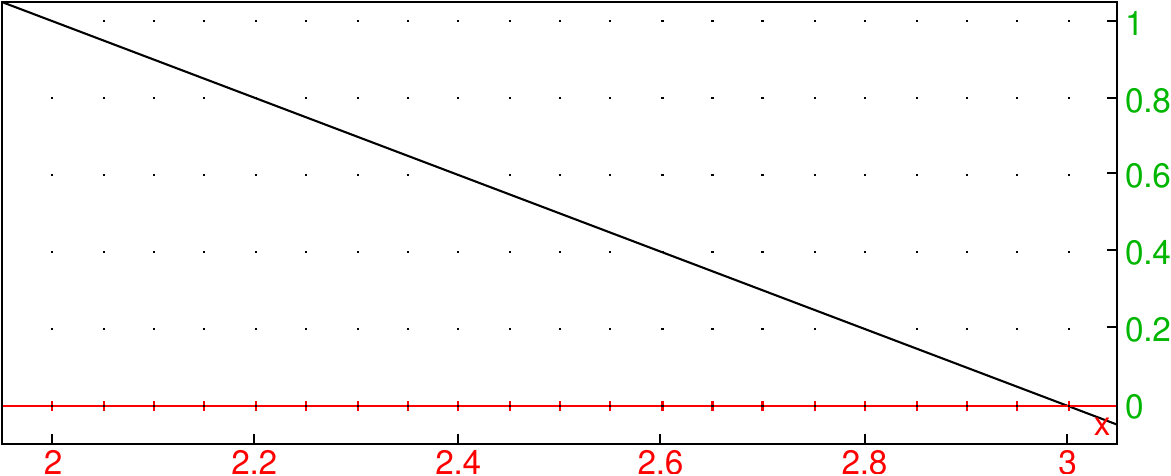
\includegraphics[width=0.75\textwidth]{xcas-DrawSlp.png}
\end{center}


\subsection{Intersection of a 2D graph with the axis}\index{solve}\index{resoudre}
\begin{itemize}
\item The ordinate of the intersection of the graph of $f$ with the 
$y$-axis is returned by :
\begin{center}{\tt f(0)}\end{center}
indeed the point of coordinates $(0,f(0))$ is the intersection point of the 
graph of $f$ with the $y$-axis,
\item Finding the intersection of the graph of $f$ with the $x$-axis 
requires solving the equation $f(x)=0$. \\
If the equation is polynomial-like, {\tt solve} will find
the exact values of the abscissa of these points. Input:
\begin{center}{\tt solve(f(x),x)}\end{center}
Otherwise, we can find numeric approximations of these 
abscissa. First look at the graph for an initial guess or a
range with an intersection and refine with {\tt fsolve}.
\end{itemize}

\section{Graph of inequalities with 2 variables : {\tt plotinequation inequationplot}}
\index{plotinequation|textbf}
\index{inequationplot|textbf}

\noindent{\tt plotinequation([f1(x,y)<a1,...fk(x,y)<ak],[x=x1..x2,y=y1..y2])} 
draws the points of the plane whose coordinates
satisfy the inequalities of 2 variables :
\[ \left\{ \begin{array}{ccc}
f1(x,y) &<&a1 \\
& ... & \\
fk(x,y)&<&ak 
\end{array}\right., \quad
x1\leq x \leq x2, y1 \leq y \leq y2 \]
Input :
\begin{center}{\tt plotinequation(x\verb|^|2-y\verb|^|2<3, [x=-2..2,y=-2..2],xstep=0.1,ystep=0.1)}\end{center}
Output :
\begin{center}{\tt the filled portion enclosing the origin and limited by the hyperbola x\verb|^|2-y\verb|^|2=3}\end{center}
Input :
\begin{center}{\tt plotinequation([x+y>3,x\verb|^|2<y], [x-2..2,y=-1..10],xstep=0.2,ystep=0.2)}\end{center}
Output :
\begin{center}{\tt the filled portion of the plane defined by -2<x<2,y<10,x+y>3,y>x\verb|^|2}\end{center}
Note that if the ranges for $x$ and $y$ are not specified, 
{\tt Xcas} takes the default values of 
{\tt X-,X+,Y-,Y+} defined in the general graphic configuration
({\tt Cfg$\blacktriangleright$Graphic configuration}).

\section{The area under a curve: \texttt{area}}
\index{area}

The \texttt{area} command takes four arguments; an expression $f(x)$,
a range for the variable $x=a..b$, an integer $n$, and the name of the
approximation method.  The approximation method can be one of
\begin{itemize}
  \item \texttt{trapezoid}
  \item \texttt{left\_rectangle}
  \item \texttt{right\_rectangle}
  \item \texttt{middle\_point}
  \item \texttt{simpson}
  \item \texttt{rombergt} (Romberg with the trapezoid method)
  \item \texttt{rombergm} (Romberg with the midpoint method)
  \item \texttt{gauss15} (The 15 point Gaussian quadrature)
\end{itemize}
\texttt{area} returns an approximation to the area under the graph
over the given interval, using the specified method with $n$
subdivisions (or $2^n$ subdivisions for \texttt{rombert},
\texttt{rombergm} and \texttt{gauss15}).\\
Input:
\begin{center}
  \tt
  area(x\^{}2,x=0..1,8,trapezoid)
\end{center}
Output:
\begin{center}
  \tt
 0.3359375 
\end{center}
Input:
\begin{center}
  \tt
  area(x\^{}2,x=0..1,8,rombergm)
\end{center}
Output:
\begin{center}
  \tt
  0.333333333333
\end{center}
Input:
\begin{center}
  \tt
  area(x\^{}2,x=0..1,3,gauss15)
\end{center}
Output:
\begin{center}
  \tt
0.333333333333
\end{center}
Input:
\begin{center}
  \tt
  area(x\^{}2,x=0..1)
\end{center}
Output:
\begin{center}
  \tt
 1/3
\end{center}

\section{Graph of the area below a curve : {\tt plotarea areaplot}}
\index{plotarea|textbf}\index{areaplot|textbf}\index{rectangle\_droit@{\sl rectangle\_droit}|textbf}\index{rectangle\_gauche@{\sl rectangle\_gauche}|textbf}\index{trapeze@{\sl trapeze}|textbf}\index{point\_milieu@{\sl point\_milieu}|textbf}

\begin{itemize}
\item With two arguments, {\tt plotarea} shades the area below a curve.\\ 
{\tt plotarea(f(x),x=a..b)} draws the area below the curve $y=f(x)$ for 
$a<x<b$, i.e. the portion of the plane defined by the inequalities $a<x<b$ and
$0<y<f(x)$ or $0>y>f(x)$ according to the sign of $f(x)$ .\\
Input :
\begin{center}{\tt plotarea(sin(x),x=0..2*pi)}\end{center}
Output :
\begin{center}{\tt the portion of plane locates in the two arches of sin(x)}\end{center}
\item With four arguments, {\tt plotarea}  represents a numeric approximation
of the area below a curve, according to a quadrature method from the
following list:\\
{\tt trapezoid,rectangle\_left,rectangle\_right,middle\_point}.\\
For example {\tt plotarea(f(x),x=a..b,n,trapezoid)} 
draws the area of $n$ trapezoids : the 
third argument is an integer $n$, and the fourth argument is the name of the 
numeric method of integration when $[a,b]$ is cut into $n$ equal parts.\\
Input :
\begin{center}{\tt plotarea((x\verb|^|2,x=0..1,5,trapezoid)}\end{center}
If you want to display the graph of the curve in contrast
(e.g. in bold red), input :
\begin{center}{\tt plotarea(x\verb|^|2,x=0..1,5,trapezoid); 
plot(x\verb|^|2,x=0..1,display=red+line\_width\_3)}\end{center}
Output :
\begin{center}{\tt the 5 trapezoids used in the trapezoid method to approach the integral}\end{center}
Input :
\begin{center}{\tt plotarea((x\verb|^|2,x=0..1,5,middle\_point)}\end{center}
Or with the graph of the curve in bold red, input :
\begin{center}{\tt plotarea(x\verb|^|2,x=0..1,5,middle\_point); plot(x\verb|^|2,x=0..1,display=red+line\_width\_3)}\end{center}
Output :
\begin{center}{\tt the 5 rectangles used in the middle\_point method
    to approach the integral}\end{center}
\end{itemize}

\section{Contour lines: {\tt plotcontour contourplot DrwCtour}}\index{plotcontour|textbf}\index{contourplot|textbf}\index{DrwCtour|textbf}\label{sec:plotcontour}
\noindent{\tt plotcontour(f(x,y),[x,y])} (or {\tt DrwCtour(f(x,y),[x,y])} or \\
 {\tt contourplot(f(x,y),[x,y])})
draws the contour lines of the surface defined by $z=f(x,y)$ for $z=-10$, 
$z=-8$, .., $z=0$, $z=2$, .., $z=10$. You may specify the desired contour
lines by a list of values of $z$ given as third argument.\\
Input :
\begin{center}{\tt  plotcontour(x\verb|^|2+y\verb|^|2,[x=-3..3,y=-3..3],[1,2,3], display=[green,red,black]+[filled\$3])}\end{center}
Output :
\begin{center}{\tt  the graph of the three ellipses x\verb|^|2-y\verb|^|2=n for n=1,2,3; the zones between these ellipses are filled with the color green,red or black}\end{center}
Input :
\begin{center}{\tt  plotcontour(x\verb|^|2-y\verb|^|2,[x,y])}\end{center}
Output :
\begin{center}{\tt  the graph of 11 hyperbolas x\verb|^|2-y\verb|^|2=n for n=-10,-8,..10}\end{center}

If you want to draw the surface in 3-d representation, 
input {\tt plotfunc(f(x,y),[x,y])}, see \ref{sec:plotfunc3}):
\begin{center}{\tt plotfunc( x\verb|^|2-y\verb|^|2,[x,y])}\end{center}
Output :
\begin{center}{\tt A 3D representation of z=x\verb|^|2+y\verb|^|2}\end{center}

\section{2-d graph of a 2-d function with colors : 
{\tt plotdensity densityplot}}
\index{plotdensity|textbf}\index{densityplot|textbf}
\noindent{\tt plotdensity(f(x,y),[x,y])}  or  {\tt densityplot(f(x,y),[x,y])}
draws the graph of $z=f(x,y)$ in the plane where the values of
$z$ are represented by the rainbow colors. The optional argument
{\tt z=zmin..zmax} specifies the range of $z$ corresponding to the
full rainbow, if it is not specified, it is deduced from the minimum
and maximum value of $f$ on the discretization. The discretization
may be specified by optional {\tt xstep=...} and {\tt ystep=...}
or {\tt nstep=...} arguments.\\
Input :
\begin{center}{\tt plotdensity(x\verb|^|2-y\verb|^|2,[x=-2..2,y=-2..2], xstep=0.1,ystep=0.1)}\end{center}
Output :
\begin{center}{\tt A 2D graph where each hyperbola defined by
    x\verb|^|2-y\verb|^|2=z has a color from the rainbow}\end{center}
{\bf Remark} : A rectangle representing the scale of colors is 
displayed below the graph.

\section{Implicit graph: {\tt plotimplicit implicitplot}}\index{plotimplicit}\index{implicitplot}\index{unfactored}
\noindent{\tt plotimplicit} or {\tt implicitplot} draws curves or 
surfaces defined by an implicit expression or equation. 
If the option {\tt unfactored} is given as last argument, the
original expression is taken unmodified. Otherwise,
the expression is normalized, then replaced by the
factorization of the numerator of its normalization.

Each factor of the expression corresponds to a component
of the implicit curve or surface. For each factor,
Xcas tests if it is of total
degree less or equal to 2, in that case {\tt conic} or
{\tt quadric} is called. Otherwise the numeric implicit solver
is called. 

Optional step and ranges arguments may be passed to the numeric
implicit solver, note that they are dismissed for each component
that is a conic or a quadric.

\subsection{2D implicit curve}\label{sec:implicitplot}
\begin{itemize}
\item {\tt plotimplicit(f(x,y),x,y)} draws the graphic representation of the
curve defined by the implicit equation $f(x,y)=0$ when $x$ (resp. $y$) 
is in {\tt WX-, WX+} (resp. in {\tt WY-, WY+}) defined by {\tt cfg}, 

\item {\tt plotimplicit(f(x,y),x=0..1,y=-1..1)} draws the graphic 
representation of the curve defined by the implicit equation $f(x,y)=0$ 
when $0\leq x \leq 1$ and $-1\leq y \leq 1$
\end{itemize} 
It is possible to add two arguments to specify the discretization
steps for $x$ 
and $y$ with {\tt xstep=...} and {\tt ystep=...}.\\
Input :
\begin{center}{\tt plotimplicit(x\verb|^|2+y\verb|^|2-1,x,y)}\end{center}
or :
\begin{center}{\tt plotimplicit(x\verb|^|2+y\verb|^|2-1,x,y,unfactored)}\end{center}
Output :
\begin{center}{\tt The unit circle}\end{center}
Input :
\begin{center}{\tt plotimplicit(x\verb|^|2+y\verb|^|2-1,x,y,xstep=0.2,ystep=0.3)}\end{center}
or :
\begin{center}{\tt plotimplicit(x\verb|^|2+y\verb|^|2-1,[x,y],xstep=0.2,ystep=0.3)}\end{center}
or :
\begin{center}{\tt plotimplicit(x\verb|^|2+y\verb|^|2-1,[x,y], xstep=0.2,ystep=0.3,unfactored)}\end{center}
Output :
\begin{center}{\tt The unit circle}\end{center}
Input :
\begin{center}{\tt plotimplicit(x\verb|^|2+y\verb|^|2-1,x=-2..2,y=-2..2, xstep=0.2,ystep=0.3)}\end{center}
Output :
\begin{center}{\tt The unit circle}\end{center}

\subsection{3D implicit surface}\label{sec:implicitplot3}
\begin{itemize}
\item {\tt plotimplicit(f(x,y,z),x,y,z)} draws the graphic 
representation of the surface defined by the implicit equation $f(x,y,z)=0$, 
\item {\tt plotimplicit(f(x,y,z),x=0..1,y=-1..1,z=-1..1)} draws the surface 
defined by the implicit equation $f(x,y,z)=0$, 
where $0\leq x \leq 1$, $-1\leq y \leq 1$ and $-1\leq z \leq 1$.
\end{itemize}
It is possible to add three arguments to specify the discretization
steps used for $x$, $y$ and $z$ with {\tt xstep=...}, {\tt ystep=...} and 
{\tt zstep=...}.\\
Input :
\begin{center}{\tt plotimplicit(x\verb|^|2+y\verb|^|2+z\verb|^|2-1,x,y,z, xstep=0.2,ystep=0.1,zstep=0.3)}\end{center}
Input :
\begin{center}{\tt plotimplicit(x\verb|^|2+y\verb|^|2+z\verb|^|2-1,x,y,z, xstep=0.2,ystep=0.1,zstep=0.3,unfactored)}\end{center}
Output :
\begin{center}{\tt The unit sphere}\end{center}
Input :
\begin{center}{\tt plotimplicit(x\verb|^|2+y\verb|^|2+z\verb|^|2-1,x=-1..1,y=-1..1,z=-1..1)}\end{center}
Output :
\begin{center}{\tt The unit sphere}\end{center}


\section{Parametric curves and surfaces : {\tt plotparam paramplot DrawParm}}\index{plotparam|textbf}\index{paramplot|textbf}\index{DrawParm|textbf}
\subsection{2D parametric curve }
\noindent {\tt plotparam([f(t),g(t)],t)}
or {\tt plotparam(f(t)+i*g(t),t)} (resp. 
{\tt plotparam(f(t)+i*g(t),t=t1..t2)})
draws the parametric representation of the curve 
defined by  $x=f(t),y=g(t)$ 
with the default range of values of $t$ (resp. for $t1 \leq t\leq t2$).\\
The default range of values is taken as specified 
in the graphic configuration ({\tt t-} and {\tt t+}, 
cf. \ref{ssec:confgraph}).
{\tt plotparam} accepts an optional argument to specify the discretization
step for $t$ with {\tt tstep=}.\\ 
Input :
\begin{center}{\tt plotparam(cos(x)+i*sin(x),x) }\end{center}
or :
\begin{center}{\tt plotparam([cos(x),sin(x)],x) }\end{center}
Output :
\begin{center}{\tt The unit circle}\end{center}
If in the graphic configuration {\tt t} goes from -4 to 1, input :
\begin{center}{\tt plotparam(sin(t)+i*cos(t))}\end{center}
or :
\begin{center}{\tt plotparam(sin(t)+i*cos(t),t=-4..1) }\end{center}
or :
\begin{center}{\tt plotparam(sin(x)+i*cos(x),x=-4..1) }\end{center}
Output :
\begin{center}{\tt the arc (sin(-4)+i*cos(-4),sin(1)+i*cos(1)) of the unit circle}\end{center}
If in the graphic configuration {\tt t} goes from -4 to 1, input :
\begin{center}{\tt plotparam(sin(t)+i*cos(t),t,tstep=0.5)}\end{center}
or :
\begin{center}{\tt plotparam(sin(t)+i*cos(t),t=-4..1,tstep=0.5)}\end{center}
Output :
\begin{center}{\tt A polygon approaching the arc (sin(-4)+i*cos(-4),sin(1)+i*cos(1)) of the unit circle}\end{center}



\subsection{3D parametric surface : {\tt plotparam paramplot DrawParm}}\index{plotparam}\index{paramplot}\index{DrawParm}
\noindent{\tt plotparam} takes two main arguments,
a list of three 
expressions of two variables and the list of these variable names
where each variable name may be replaced by variable=interval
to specify the range of the parameters.
It accepts an optional argument to specify
the discretization steps of the parameters $u$ and $v$ with 
{\tt ustep=...} and {\tt vstep=...}.\\
{\tt plotparam([f(u,v),g(u,v),h(u,v)],[u,v])} draws the surface defined by the 
first argument : $x=f(u,v),y=g(u,v),z=h(u,v)$, where $u$ and $v$
ranges default to the graphic configuration.\\
Input :
\begin{center}{\tt plotparam([v*cos(u),v*sin(u),v],[u,v])}\end{center}
Output :
\begin{center}{\tt The cone $x=v*\cos(u),y=v*\sin(u),z=v$}\end{center}
To specify the range of each parameters, replace each variable
by an equation variable=range, like this:
\begin{center}{\tt plotparam([v*cos(u),v*sin(u),v],[u=0..pi,v=0..3]) }\end{center}
Output :
\begin{center}{\tt A portion of the cone $x=v*\cos(u),y=v*\sin(u),z=v$}\end{center}
Input :
\begin{center}{\tt plotparam([v*cos(u),v*sin(u),v],[u=0..pi,v=0..3],ustep=0.5,vstep=0.5)}\end{center}
Output :
\begin{center}{\tt A portion of the cone $x=v*\cos(u),y=v*\sin(u),z=v$}\end{center}
 
\section{Bezier curves: \texttt{bezier}}\index{bezier}

The \texttt{bezier} command takes as argument a sequence \texttt{L} of
points.\\
\texttt{bezier(L,plot)} plots the Bezier curve with the given control
points.

If the points are $P_0,P_1,\dots,P_n$, the Bezier curve is the curve
parameterized by $\sum_{j=0}^{n} \binom{n,j} t^j (1-t)^{n-j} P_{j}$.

\noindent
Input:
\begin{center}
  \tt
  bezier(1,1+i,2+i,3-i,plot)
\end{center}
Output:
\begin{center}
   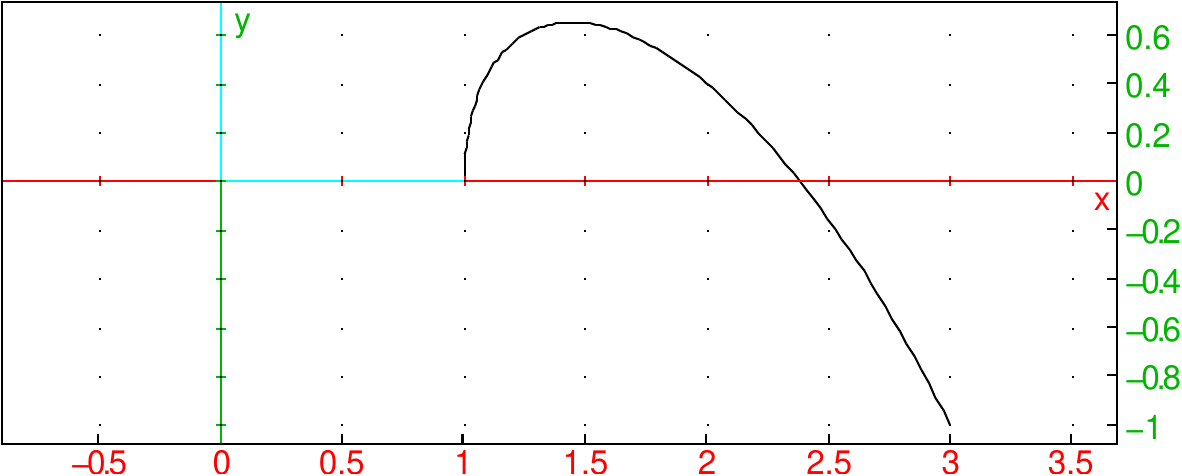
\includegraphics[width=0.75\textwidth]{xcas-bezier1.png}
\end{center}
Input:
\begin{center}
  \tt
  bezier(point(0,0,0),point(1,1,0),point(0,1,1),plot)
\end{center}
Output:
\begin{center}
   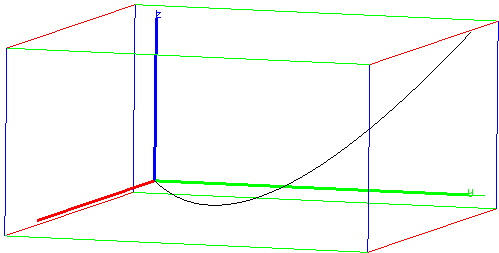
\includegraphics[width=0.75\textwidth]{xcas-bezier2.png}
\end{center}

To get the parameterization of the curve, you can use \texttt{parameq}.\\
Input:
\begin{center}
  \tt
   parameq(bezier(1,1+i,2+i,3-i))
\end{center}
Output:
\begin{center}
  \tt
  (1-t)\^{}3+3*t*(1-t)\^{}2*(1+i)+3*t\^{}2*(1-t)*(2+i)+t\^{}3*(3-i)  
\end{center}
Input:
\begin{center}
  \tt
    parameq(bezier(point([0,0,0]),point([1,1,0]),point([0,1,1])))
\end{center}
Output:
\begin{center}
  \tt
    point[2*t*(1-t),2*t*(1-t)+t\^{}2,t\^{}2]
\end{center}
 
\section{Curve defined in polar coordinates : {\tt plotpolar polarplot DrawPol courbe\_polaire}}\index{plotpolar|textbf}\index{polarplot|textbf}\index{DrawPol|textbf}\index{courbe\_polaire|textbf}
\noindent Let $E_t$ be an expression depending on the variable $t$.\\
{\tt plotpolar($E_t$,t)} draws the polar representation of the
curve defined by $\rho=E_t$ for $\theta=t$, that is
in cartesian coordinates the curve $(E_t \cos(t),E_t \sin(t))$.
The range of the parameter may be specified by replacing the second argument
by {\tt t=tmin..tmax}. The discretization parameter may be specified
by an optional {\tt tstep=...} argument.\\
Input 
\begin{center}{\tt  plotpolar(t,t)}\end{center}
Output :
\begin{center}{\tt The spiral $\rho$=t is plotted}\end{center}
Input
\begin{center}{\tt  plotpolar(t,t,tstep=1)}\end{center}
or :
\begin{center}{\tt  plotpolar(t,t=0..10,tstep=1)}\end{center}
Output :
\begin{center}{\tt A polygon line approaching the spiral $\rho$=t is plotted}\end{center}

\section{Graph of a recurrent sequence : {\tt plotseq seqplot graphe\_suite}}\index{plotseq}\index{seqplot}\index{graphe\_suite}\label{sec:plotseq}
\noindent Let $f(x)$ be an expression depending on the variable $x$ 
(resp. $f(t)$ an expression depending on the variable $t$).\\
{\tt plotseq($f(x)$,a,n)} (resp. {\tt plotseq($f(t)$,t=a,n)}) draws the line 
$y=x$, the graph of $y=f(x)$ (resp. $y=f(t)$) and the $n$ first terms of the
recurrent sequence defined by : $u_0=a,\ \ u_n=f(u_{n-1})$.
The $a$ value may be replaced by a list of 3 elements, $[a,x_-,x_+]$
where $x_-..x_+$ will be passed as $x$ range for the graph computation.\\ 
Input :
\begin{center}{\tt plotseq(sqrt(1+x),x=[3,0,5],5)}\end{center}
Output :
\begin{center}{\tt the graph of y=sqrt(1+x), of y=x and of the 5 first terms of the sequence u\_0=3 and u\_n=sqrt(1+u\_(n-1))}\end{center}

\section{Tangent field : {\tt plotfield fieldplot}}\index{plotfield}\index{fieldplot}
\begin{itemize}
\item Let $f(t,y)$ be an expression depending on two variables $t$ and $y$, 
then :
\begin{center}
{\tt plotfield(f(t,y),[t,y])}
\end{center} 
draws the tangent field of the 
differential equation $y'=f(t,y)$ where $y$ is a real variable and
where $t$ is the abscissa,
\item Let $V$ be 
a vector of two expressions depending on 2 variables $x,y$ but 
independent of the time $t$, then 
\begin{center}
{\tt plotfield(V,[x,y])}
\end{center}
draws the vector field $V$,
\item The range of values of $t,y$ or of $x,y$ can be specified with\\
{\tt t=tmin..tmax}, {\tt x=xmin..xmax}, {\tt y=ymin..ymax}\\
in place of the variable name.
\item The discretization may be specified with optional
arguments {\tt xstep=...}, {\tt ystep=...}.
\end{itemize}
Input :
\begin{center}{\tt plotfield(4*sin(t*y),[t=0..2,y=-3..7]) }\end{center}
Output :
\begin{center}{\tt Segments with slope 4*sin(t*y), representing tangents, are plotting in different points}\end{center}
With two variables $x,y$, input :
\begin{center}
{\tt plotfield(5*[-y,x],[x=-1..1,y=-1..1]) }
\end{center}

\section{Plotting a solution of a differential equation : {\tt plotode odeplot}}\index{plotode}\index{odeplot}
\noindent Let $f(t,y)$ be an expression depending on two variables 
$t$ and $y$.
\begin{itemize}
\item {\tt plotode($f(t,y)$,[t,y],[t0,y0])} draws the solution of 
the differential equation $y'=f(t,y)$ crossing through 
the point {\tt (t0,y0)} (i.e. such that $y(t_0)=y_0$)
\item
By default, $t$ goes in both directions. The range of value of $t$
may be specified by the optional argument
{\tt t=tmin..tmax}.
\item
We can also represent, in the space or in the plane,
the solution of a differential equation 
$y'=f(t,y)$ where $y=(X,Y)$ is a vector of size 2.
Just replace  $y$ by the variable names $X,Y$
and the initial value $y_0$ by the two initial values of the
variables at time $t_0$.
\end{itemize}
Input :
\begin{center}{\tt plotode(sin(t*y),[t,y],[0,1]) }\end{center}
Output :
\begin{center}{The graph of the solution of y'=sin(t,y) crossing through the point (0,1)}\end{center}
Input~:
\begin{center}
{\tt S:=odeplot([h-0.3*h*p, 0.3*h*p-p], [t,h,p],[0,0.3,0.7])}
\end{center}
Output, the graph in the space of the solution of :
\[ [h,p]'=[h-0.3 h*p, 0.3 h*p-p] \quad [h,p](0)=[0.3,0.7] \]
To have a 2-d graph (in the plane), use the option 
{\tt plane}
\begin{center}
{\tt S:=odeplot([h-0.3*h*p, 0.3*h*p-p], [t,h,p],[0,0.3,0.7],plane)}
\end{center}
To compute the values of the solution, see
the subsection \ref{ssec:odesolve}.

\section{Interactive plotting of solutions of a differential equation : {\tt interactive\_plotode interactive\_odeplot}}\index{interactive\_plotode}\index{interactive\_odeplot}
\noindent Let $f(t,y)$ be an expression depending on two 
variables $t$ and $y$.\\
{\tt interactive\_plotode(f(t,y),[t,y])} draws the tangent field
of the differential equation $y'=f(t,y)$ in a new window. 
In this window, one can click on a point to get the 
plot of the solution of $y'=f(t,y)$ crossing through this point.\\
You can further click to display 
several solutions. To stop  press
the {\tt Esc} key.\\
Input :
\begin{center}{\tt interactive\_plotode(sin(t*y),[t,y]) }\end{center}
Output :
\begin{center}{\tt The tangent field is plotted with the
    solutions of y'=sin(t,y) crossing through the points defined by
     mouse clicks}\end{center}

\section{Animated graphs (2D, 3D or "4D")}
{\tt Xcas} can display animated 2D, 3D or "4D" graphs. 
This is done first by computing
a sequence of graphic objects, then after completion,
by displaying the sequence in a loop.
\begin{itemize} 
\item To stop or start again the animation, click on the button 
$\blacktriangleright \mid$ (at the left of {\tt Menu}).
\item
The display time of each graphic object is specified in {\tt animate} of the
graph configuration ({\tt cfg} button). Put a small time, 
to have a fast animation.
\item
If {\tt animate} is {\tt 0}, the animation is frozen,
you can move in the sequence of objects one by one by clicking
on the mouse in the graphic scene.
\end{itemize}

\subsection{Animation of a 2D graph~: {\tt animate}}\index{animate}
\noindent{\tt animate} can create a 2-d animation with graphs of functions
depending on a parameter. The parameter is specified as the 
third argument of 
{\tt animate}, the number of pictures as fourth argument with
{\tt frames=}\index{frames@{\sl frames}|textbf}number, 
the remaining arguments are the same as those of the {\tt plot} command, 
see section \ref{sec:plot2d}, p. \pageref{sec:plot2d}.\\
Input :
\begin{center}
{\tt animate(sin(a*x),x=-pi..pi,a=-2..2,frames=10,color=red)}
\end{center}
Output :
\begin{center}{\tt a sequence of graphic representations of y=sin($a$x) for 
11 values of $a$ between -2 and 2}\end{center}

\subsection{Animation of a 3D graph~: {\tt animate3d}}\index{animate3d}
\noindent{\tt animate3d} can create a 3-d animation with 
function graphs depending on a parameter. The parameter is specified as
the third argument of {\tt animate3d}, the number of pictures
as fourth argument with 
{\tt frames=}\index{frames@{\sl frames}}number, the remaining arguments
are the same as those of the {\tt plotfunc} command, see
section \ref{sec:plotfunc3}, p. \pageref{sec:plotfunc3}.\\
Input :
\begin{center}
{\tt animate3d(x\verb|^|2+a*y\verb|^|2,[x=-2..2,y=-2..2],a=-2..2, frames=10,display=red+filled)}
\end{center}
Output :
\begin{center}{\tt a sequence of graphic representations
 of z=x\verb|^|2+$a$*y\verb|^|2 for 11 values of $a$ between -2 and 2}
\end{center}

\subsection{Animation of a sequence of graphic objects~: {\tt animation}}\index{animation}
\noindent{\tt animation} animates the representation of a
sequence of graphic objects
with a given display time. The sequence of objects depends most of
the time on a parameter and is defined using the {\tt seq} command
but it is not mandatory.\\
{\tt animation} takes as argument the sequence of graphic objects.\\
To define a sequence of graphic objects with {\tt seq},
enter the definition of the graphic object (depending on
the parameter), the parameter name, its minimum value, its
 maximum value maximum and optionally a step value.\\
Input :
\begin{center}{\tt animation(seq(plotfunc(cos(a*x),x),a,0,10))}\end{center}
Output :
\begin{center}{\tt The sequence of the curves defined by $y=\cos(ax)$, for $a=0,1,2..10$}\end{center}
Input :
\begin{center}
{\tt animation(seq(plotfunc(cos(a*x),x),a,0,10,0.5))}
\end{center}
or :
\begin{center}
{\tt animation(seq(plotfunc(cos(a*x),x),a=0..10,0.5))}
\end{center}
Output :
\begin{center}{\tt The sequence of the curves defined by $y=\cos(ax)$, for $a=0,0.5,1,1.5..10$ }\end{center}
Input :
\begin{center}{\tt animation(seq(plotfunc([cos(a*x),sin(a*x)],x=0..2*pi/a), a,1,10))}\end{center}
Output :
\begin{center}{\tt The sequence of two curves defined by $y=\cos(ax)$ and $y=\sin(ax)$, for $a=1..10$ and for $x=0..2\pi/a$ }\end{center}
Input :
\begin{center}{\tt animation(seq(plotparam([cos(a*t),sin(a*t)], t=0..2*pi),a,1,10))}\end{center}
Output :
\begin{center}{\tt The sequence of the parametric curves defined by  $x=\cos(at)$ and $y=\sin(at)$, for $a=1..10$ and for $t=0..2\pi$ }\end{center}
Input :
\begin{center}{\tt animation(seq(plotparam([sin(t),sin(a*t)], t,0,2*pi,tstep=0.01),a,1,10))}\end{center}
Output :
\begin{center}{\tt The sequence of the parametric curves defined by $x=\sin(t),y=\sin(at)$, for $a=0..10$ and $t=0..2\pi$}\end{center}
Input :
\begin{center}{\tt animation(seq(plotpolar(1-a*0.01*t\verb|^|2, t,0,5*pi,tstep=0.01),a,1,10))}\end{center}
Output :
\begin{center}{\tt The sequence of the polar curves defined by $\rho=1-a*0.01*t^2$, for $a=0..10$ and $t=0..5\pi$}\end{center}
Input :
\begin{center}{\tt plotfield(sin(x*y),[x,y]); animation(seq(plotode(sin(x*y),[x,y],[0,a]),a,-4,4,0.5))}\end{center}
Output :
\begin{center}{\tt The tangent field of y'=sin(xy) and the sequence of the integral curves crossing through the point $(0,a)$ for $a$=-4,-3.5...3.5,4}\end{center}
Input :
\begin{center}{\tt animation(seq(display(square(0,1+i*a),filled),a,-5,5))}\end{center}
Output :
\begin{center}{\tt The sequence of the squares defined by the points 0 and 1+i*$a$ for $a=-5..5$}\end{center}
Input :
\begin{center}{\tt animation(seq(droite([0,0,0],[1,1,a]),a,-5,5))}\end{center}
Output :
\begin{center}{\tt The sequence of the lines defined by the points [0,0,0] and [1,1,$a$] for $a=-5..5$}\end{center}
Input :
\begin{center}{\tt animation(seq(plotfunc(x\verb|^|2-y\verb|^|a,[x,y]),a=1..3))}\end{center}
Output :
\begin{center}{\tt The sequence of the "3D" surface defined by $x^2-y^a$, for $a=1..3$ with rainbow colors}\end{center}
Input :
\begin{center}{\tt animation(seq(plotfunc((x+i*y)\verb|^|a,[x,y], display=filled),a=1..10)}\end{center}
Output :
\begin{center}{\tt The sequence of the "4D" surfaces defined by $(x+i*y)^a$, for $a=0..10$ with rainbow colors}\end{center}

{\bf Remark}
We may also define the sequence with a program, 
for example if we want to draw the
segments of length $1,\sqrt 2...\sqrt 20$ constructed with a 
right triangle of side 1 and the previous segment
(note that there is a {\tt c:=evalf(..)} statement
to force approx. evaluation otherwise the computing time 
would be too long) :
\begin{verbatim}
seg(n):={
 local a,b,c,j,aa,bb,L;
 a:=1;
 b:=1;
 L:=[point(1)];
 for(j:=1;j<=n;j++){
  L:=append(L,point(a+i*b));
  c:=evalf(sqrt(a^2+b^2));
  aa:=a;
  bb:=b;
  a:=aa-bb/c;
  b:=bb+aa/c;
 }
 L;
}
\end{verbatim}
Then input : 
\begin{center}{\tt animation(seg(20))}\end{center}
We see, each point, one to one with a display time that
depends of the {\tt animate} value in {\tt cfg}.\\
or :
\begin{center}{\tt L:=seg(20); s:=segment(0,L[k])\$(k=0..20)}\end{center}
We see 21 segments. \\
Then, input :
\begin{center}{\tt animation(s)}\end{center}
We see, each segment, one to one with a display time that
depends of the {\tt animate} value in {\tt cfg}.

\chapter{Statistics}\label{sec:stat}

\section{One variable statistics}

\texttt{Xcas} has several functions to perform statistics; the data is
typically given as a list of numbers, such as \texttt{A :=
[0,1,2,3,4,5,6,7,8,9,10,11]}.  We will use this particular list in
several examples. Section \ref{sec:statmat} will discuss statistics on
matrices.

\subsection{The mean: \texttt{mean}\index{mean}}

Recall that the mean of a list $x_1,\dots,x_n$ is simply their numeric
average $(x_1 + \cdots + x_n)/n$.  \texttt{Xcas} can calculate the
mean of a list of numbers with the \texttt{mean} command.
If you enter 
\begin{center}
  \tt
  mean([1,2,3,4])
\end{center}
then you will get
\begin{center}
  \tt 
  5/2
\end{center}
since $(1+2+3+4)/4 = 5/2$.
If you give \texttt{mean} a matrix as an argument, then it will return a
list with the numeric average of each column;
\begin{center}
  \tt
  mean([[1,2,3],[5,6,7]])  
\end{center}
will return
\begin{center}
  \tt
  [3,4,5]
\end{center}
since $(1+5)/2 = 3$, $(2+6)/2 = 4$ and $(3 + 7)/2 = 5$.

To get the weighted average of a list of numbers you can give
\texttt{mean} a second argument, which should be a list of the
weights.  For example,
\begin{center}
  \tt
  mean([2,4,6,8],[2,2,3,3])
\end{center}
will return
\begin{center}
  \tt
  27/5
\end{center}
since $(2\cdot 2 + 4\cdot 2 + 6\cdot 3 + 8\cdot 3)/(2 + 2 + 3 + 3) =
27/5$.
Similarly, you can find the weighted average of the columns of a
matrix by giving \texttt{mean} a second argument of a matrix of
weights.  If you enter
\begin{center}
  \tt
  mean([[1,2],[3,4]],[[1,2],[2,1]])
\end{center}
then you will get
\begin{center}
  \tt
  [7/3,8/3]
\end{center}
since $(1\cdot 1 + 3\cdot 2)/(1+2) = 7/3$ and $(2\cdot 2 + 4\cdot 1)/(2 +
1) = 8/3$.

\subsection{Variance and standard deviation: \texttt{variance}\index{variance} \texttt{stdev}\index{stdev}}

The variance of a list of numbers measures how close the numbers are
to their mean by finding the average of the squares of the
differences between the numbers and the mean; specifically,
given a list of numbers $[x_1,\dots,x_n]$ with mean $\mu = (x_1 +
\cdots + x_n)/n$, the variance is
\[
\frac{(x_1 - \mu)^2 + \dots + (x_n - \mu)^2}{n}.
\]
The squares help ensure that the numbers above the mean and those
below the mean don't cancel out.  The variance can be computed with
the command \texttt{variance},

A potentially better way to measure how close numbers are to their
mean is the standard deviation, which is the square root of the
variance;.  Note that if the list of numbers have units, then the
standard deviation will have the same unit.
The \texttt{stddev} function will compute the standard
deviation of a list of numbers.  For example, 
the list $[1,2,3,4]$ has mean $5/2$, and so 
\texttt{stddev([1,2,3,4])}
will return
\begin{center}
  \tt
  2*sqrt(5)/4
\end{center}
since
\[ \sqrt{\frac{(1-5/2)^2 + (2-5/2)^2 + (3-5/2)^2 + (4-5/2)^2}{4}} =
\frac{2\sqrt{5}}{4}
\]
Like the mean, given a matrix, \texttt{stddev} will compute the
standard deviation of each column separately;
\begin{center}
  \tt
  stddev([[1,2],[3,6]])
\end{center}
will compute
\begin{center}
  \tt
  [1,2]
\end{center}
Also, a second list (or matrix) as an argument will provide weights
when finding the standard deviation;
\begin{center}
  \tt
  stddev([1,2,3],[2,1,1])
\end{center}
will return
\begin{center}
  \tt
  4*sqrt(11)/16
\end{center}

\subsection{The population standard deviation: \texttt{stddevp}\index{stddevp} \texttt{stdDev}\index{stdDev}}

Given a large population, rather than collecting all of the numbers it
might be more feasible to get a smaller collection of numbers and try
to extrapolate from that.  For example, to get information about the
ages of a large population, you might get the ages of a sample of 100
of the people and work with that.

If a list of numbers is a sample of data from a larger population,
then the \texttt{mean} function will find the mean of the sample,
which can be used to estimate the mean of the population.  The
standard deviation uses the mean to find the standard
deviation of the sample, but since the mean of the sample is only an
approximation to the mean of the entire population, the standard
deviation of the sample doesn't provide an optimal estimate of
the standard deviation of the population.  An unbiased estimate of the
standard deviation of the entire population is given by the population
standard deviation \texttt{stddevp} function; 
given a list $L = [x_1,\dots,x_n]$ with mean $\mu$, the population
standard deviation is 
\[
\sigma = \sqrt{\frac{(x_1 - \mu)^2 + \dots + (x_n - \mu)^2}{n-1}}.
\]
Note that
\[ \text{stddevp}(L)^2 = \frac{n}{n-1} \text{stddev}(L)^2.\]

For example,
\begin{center}
  \tt
  stddev([1,2,3,4])
\end{center}
will return
\begin{center}
  \tt
  sqrt(5)/2
\end{center}
while 
\begin{center}
  \tt
  stddevp([1,2,3,4])
\end{center}
will return
\begin{center}
  \tt
  sqrt(15)/3
\end{center}

Like \texttt{stddev}, the \texttt{stddevp} command can take a second
argument for weights.  If you enter
\begin{center}
  \tt
  A := [0,1,2,3,4,5,6,7,8,9,10,11]\\
  stddevp(A,A)
\end{center}
then you will get
\begin{center}
  \tt
  sqrt(66)/3
\end{center}

The \texttt{stdDev} function is equivalent to \texttt{stddevp}, for TI
compatibility.  There is no population variance function; if needed,
it can be computed by squaring the \texttt{stddevp} function.

\subsection{The median: \texttt{median}\index{median}}

Although the average of a list of numbers typically means the mean,
there are other notions of ``average''.  Another one is the median;
the median of a list of numbers is the middle number when they are
listed in numeric order.  For example, the median of the list
$[1,2,5,7,20]$ is simply $5$.  If the length of a list of numbers is
even, so there isn't a middle number, the median is then the mean of
the two middle numbers; for example, the median of $[1,2,5,7,20,21]$ is 
$(5+7)/2 = 6$.

The \texttt{median} function finds the median of a list.  The command
\begin{center}
  \tt
  median([1,2,5,7,20])
\end{center}
will return
\begin{center}
  \tt
  5
\end{center}
The \texttt{median} function can take weights with a second argument,
where the weight of number represents how many times it is counted in
a list.  For example,
\begin{center}
  \tt
  median([1,2,5,7,20],[5,3,2,1,2])
\end{center}
will return
\begin{center}
  \tt
  2
\end{center}
since the median of $1,1,1,1,1,2,2,2,5,5,7,20,20$ is $2$.

\subsection{Quartiles: \texttt{quartiles}\index{quartiles} \texttt{quartile1}\index{quartile1} \texttt{quartile3}\index{quartile3}}

Recall that the quartiles of a list of numbers divide it into four
equal parts; the first quartile is the number $q_1$ such that
one-fourth of the list numbers fall below $q_1$; i.e., the median of
that part of the list which fall at or below the list median.  The
second quartiles is the number $q_2$ such that half of the list
numbers fall at or below $q_2$; more specifically, the median of the
list.  And of course the third quartile is the number $q_3$ such that
three-fourths of the list numbers fall at or below $q_3$.

The function \texttt{quartiles} takes a list and returns a column
vector consisting of the minimum of the list, the first quartile, the second
quartile, the third quartile and the maximum.   If you enter
\begin{center}
  \tt
  A := [0,1,2,3,4,5,6,7,8,9,10,11];\\
  quartiles(A)
\end{center}
you will get
\begin{center}
  \tt
  [[0.0],[2.0],[5.0],[8.0],[11.0]]
\end{center}

You can get the individual entries of this vector with the commands
\texttt{min}, \texttt{quartile1}, \texttt{median}, \texttt{quartile2}
and \texttt{max}.

Just as with median, the \texttt{quartiles} function can take a second
argument consisting of weights for the first argument; for example,
\begin{center}
  \tt
  quartiles(A,A)
\end{center}
would return
\begin{center}
  \tt
  [0,6,8,10,11]
\end{center}

\subsection{Quantiles: \texttt{quantile}\index{quantile}}

Similar to quartiles, a quantile of a list is the number $q$ such that
a given fraction of the list numbers fall at or below $q$.  The first
quartile, for example, is the quantile with the fraction 0.25.

The command \texttt{quantile} takes a list of numbers and a value $p$
between 0 and 1 as arguments and returns the $p$th quantile.  For
example,
\begin{center}
  \tt
  A := [0,1,2,3,4,5,6,7,8,9,10,11]\\
  quantile(A,0.1)
\end{center}
returns the quantile with $p = 0.1$ (the first decile):
\begin{center}
  \tt
  1.0
\end{center}

Like \texttt{quartile}, the \texttt{quantile} command can take an
argument representing weights of the list; the weights can be given as
a second argument and then the value $p$ will be the third.  The command
\begin{center}
  \tt
  quantile(A,A,0.25)
\end{center}
will return
\begin{center}
  \tt
  6
\end{center}

\subsection{The boxwhisker: \texttt{boxwhisker}\index{boxwhisker} \texttt{mustache}\index{mustache}}

A boxwhisker is a graphical view of the quartiles of a list of numbers.
The boxwhisker consists of a line segment from the the minimum of the
list to the first quartile, leading to a rectangle from the first
quartile to the third quartile, followed by a line segment from the
third quartile to the maximum of the list.  The rectangle will contain
a vertical segment indicating the median, and the two line segments
will contain vertical lines indicating the first and ninth decile.

The \texttt{boxwhisker} (or \texttt{mustache}) command will create a
boxwhisker for a list.  For example, if you enter
\begin{center}
  \tt
  boxwhisker([-1,1,2,2.2,3,4,-2,5])
\end{center}
a graphic window will appear showing the boxwhisker,
\begin{center}
  \includeimage{xcas-boxwhisker.png}
\end{center}

\subsection{Classes: \texttt{classes}\index{classes}}

The \texttt{classes} command can be used to groups a collection of
numbers into intervals; the result will be a list where each element
is an interval \texttt{a..b} followed by how many of the numbers are
in the interval $[a,b)$. The collection of numbers can be given as a
list or matrix.

If $L$ is a collection of numbers, $a$ and $b$ are numbers, then
\texttt{classes($L$,$a$,$b$)} will return the list
\texttt{[[$a$..$a+b$,$n_1$],[$a+b$..$a+2b$,$n_2$],...]} where each number in $L$ is
in one of the intervals $[a+kb, a+(k+1)b)$ and $n_k$ is
how many numbers from $L$ are in the corresponding interval.  For
example,
\begin{center}
  \tt
  classes([0,0.5,1,1.5,2,2.5,3,3.5,4],0,2)
\end{center}
will return
\begin{center}
  \tt
  [[0.0 .. 2.0,4],[2.0 .. 4.0,4],[4.0 .. 6.0,1]]
\end{center}
while 
\begin{center}
  \tt
  classes([0,0.5,1,1.5,2,2.5,3,3.5,4],-1,2)
\end{center}
will return
\begin{center}
  \tt
  [[(-1.0) .. 1.0,2],[1.0 .. 3.0,4],[3.0 .. 5.0,3]]
\end{center}
If the numbers $a$ and $b$ are omitted, they will default to the
configurable values of \texttt{class\_min} and \texttt{class\_size},
which default to $0$ and  $1$.

Another way to split the list $L$ into intervals is by making the
third argument the midpoints of the desired intervals.  For example,
if you enter
\begin{center}
  \tt
  classes([0,0.5,1,1.5,2,2.5,3,3.5,4],1,[1,3,5])
\end{center}
you will get
\begin{center}
  \tt
  [[0.0..2.0,4],[2.0..4.0,4],[4.0..6.0,1]]
\end{center}

Finally, you can simply state the intervals that you want to use by
giving them as a list for the second argument.  In this case, not
every number in the list is necessarily in one of the intervals.  If
you enter
\begin{center}
  \tt
  classes([0,0.5,1,1.5,2,2.5,3,3.5,4],[1..3,3..6])
\end{center}
you will get
\begin{center}
  \tt
  [[1 .. 3,4],[3 .. 6,3]]
\end{center}

\subsection{Histograms: \texttt{histogram}\index{histogram} \texttt{histogramme}\index{histogramme}}

Given a list of intervals and a number of points in each interval,
such as is given by the output of the \texttt{classes} command, the
\texttt{histogram} (or \texttt{histogramme}) command will draw a box
over each interval so that the height of each box is proportional to
the number of points and the total area of the boxes is 1.  For
example, if you enter
\begin{center}
  \tt
  histogram([[1.5..1.65,50],[1.65..1.7,20],[1.7..1.8,30]])
\end{center}
you will get
\begin{center}
  \includeimage{xcas-histogram1.png}
\end{center}

If you just give the \texttt{histogram} a list of numbers, or a list
with values $a$ and $b$, then you will get the histogram of the result
of applying \texttt{classes} to the list.
% will start at 0 and draw boxes over intervals of width 1, such that
% the height of the boxes are proportional to the number of list
% elements in the interval and the total area will be 1.  For example,
% if you enter
% \begin{center}
%   \tt
%   histogram([1,2,2.5,2.5,3])
% \end{center}
% you will get
% PIC HISTOGRAM1
% You can change the starting point and interval width (from 0 and 1,
% respectively) by giving \texttt{histogram} second and third arguments;
For example, if you enter
\begin{center}
  \tt
  histogram([1,2,2.5,2.5,3],0.5,0.75)
\end{center}
you will get
\begin{center}
  \includeimage{xcas-histogram2.png}
\end{center}

\subsection{Accumulating terms:
\texttt{accumulate\_head\_tail}\index{accumulate\_head\_tail}}

The first terms and last terms of a list can be accumulated by
replacing them with their sum using the \texttt{accumulate\_head\_tail}
command.  This command takes the list, the number of initial terms to
sum, and the number of end terms to add, and returns the list with the
initial terms and end terms replaced by their sums.  For example, the
command
\begin{center}
  \tt
  accumulate\_head\_tail([1,2,3,4,5,6,7,8,9,10],3,4)
\end{center}
will return
\begin{center}
  \tt
  [6,4,5,6,34]
\end{center}

\subsection{Frequencies: \texttt{frequencies}\index{frequencies} \texttt{frequences}\index{frequences}}

Given a list of numbers, the \texttt{frequencies} (or
\texttt{frequences}) command  will return
the numbers in the list with their frequencies; i.e., the fraction of
list items equal to the number. For example,
\begin{center}
  \tt
  frequencies([1,2,1,1,2,1,2,4,3,3])
\end{center}
will return
\begin{center}
  \tt
  [[1,0.4],[2,0.3],[3,0.2],[4,0.1]]
\end{center}

You can use this, for example, to simulate flipping a fair coin and
seeing how many times each side appears; to flip a coin 1000 times,
for example, you can enter
\begin{center}
  \tt
  frequencies([rand(2) \$ (k=1..1000)])
\end{center}
and you might get
\begin{center}
  \tt
  [[0,0.513],[1,0.487]]
\end{center}

\subsection{Cumulative frequencies: \texttt{cumulated\_frequencies}\index{cumulated\_frequencies} \texttt{frequences\_cumulees}\index{frequences\_cumulees}}

Given a list, the \texttt{cumulated\_frequencies} command will plot
the cumulated frequency of the numbers in the list; i.e., the area
under the resulting graph at a value $x$ will be the fraction of
numbers less than $x$.  For example, if you enter
\begin{center}
  \tt
  cumulated\_frequencies([1,2,1,1,2,1,2,4,3,3])
\end{center}
then you will get
\begin{center}
  \includeimage{xcas-cumfreq1.png}
\end{center}

The \texttt{cumulated\_frequencies} command can also take a matrix
with two columns as an argument.  In this case, the first column will
represent values while the second column will represent the number of
times the values occur.  For example, the above graph can be drawn
with the command
\begin{center}
  \tt
    cumulated\_frequencies([[1,4],[2,3], [3,2], [4,1]])
\end{center}

If the first column of the input matrix contains intervals
\texttt{$a$..$b$} instead of numbers, then the second column values will
be normalized to add up to one, and will represent the frequencies of
the intervals.  If the matrix has the form 
\[ [[a_0..a_1,f_1],...,[a_{n-1}..a_n,f_n]] \]
then the plot will consist of the polygonal path starting at $(a_0,0)$
and moving to $(a_1,f_1)$ to $(a_2,f_1+f_2)$ and so on until
$(a_n,f_1+\cdots + f_n)$.  For example, both
\begin{center}
  \tt
  cumulated\_frequencies([[1..2,30],[2..4,40],[4..5,30]])
\end{center}
and
\begin{center}
  \tt
  cumulated\_frequencies([[1..2,03],[2..4,0.4],[4..5,0.3]])
\end{center}
will give you
\begin{center}
  \includeimage{xcas-cumfreqint.png}
\end{center}

If the matrix given to \texttt{cumulated\_frequencies} has more than
two columns, then each additional column will represent a different
distribution of the numbers in the first column, and each distribution
will be graphed.  For example, if you enter
\begin{center}
  \tt
    cumulated\_frequencies([[1,4,1],[2,3,4], [3,2,1], [4,1,2]])
\end{center}
then both the distributions given by 
\texttt{[[1,4],[2,3], [3,2], [4,1]]}
and
\texttt{[[1,1],[2,4], [3,1], [4,2]]}
will be drawn on the same axes; the result will be
\begin{center}
  \includeimage{xcas-cumfreq2.png}
\end{center}

\subsection{Bar graphs: \texttt{bar\_plot}\index{bar\_plot}}

You can draw bar graphs with the \texttt{bar\_plot} command.  You give
it a list, whose elements are pairs of labels and values, and the
result will be a bar graph with a bar for each label, whose height is
given by the corresponding value.  For example, if you enter
\begin{center}
  \tt
  bar\_plot([["France", 6],["Germany", 12], ["Switzerland", 5]])
\end{center}
you will get
\begin{center}
  \includeimage{xcas-barplot1.png}
\end{center}

If you have more than one set of values for each label, you can use
\texttt{bar\_plot} to draw several bar graphs at the same time by
including all values for each label, with a list of identifiers for
the bar graphs given by the first argument.  If you enter
\begin{center}
  \tt
  bar\_plot([[2,"xyz","abc"],["A",2,5],["B",5,6],["C",6,6]])
\end{center}
you will get
\begin{center}
  \includeimage{xcas-barplot2.png}
\end{center}

\subsection{Pie charts: \texttt{camembert}\index{camembert}}

You can draw pie charts using the same structure as bar graphs, but
with the command \texttt{camembert}.  If you enter
\begin{center}
  \tt
  camembert([["France", 6],["Germany", 12], ["Switzerland", 5]])
\end{center}
you will get
\begin{center}
  \includeimage{xcas-piechart1.png}
\end{center}
and if you enter
\begin{center}
  \tt
  camembert([[2,"xyz","abc"],["A",2,5],["B",5,6],["C",6,6]])
\end{center}
you will get
\begin{center}
  \includeimage{xcas-piechart2.png}
\end{center}

\section{Two variable statistics}

\subsection{Covariance and correlation: \texttt{covariance}\index{covariance} \texttt{correlation}\index{correlation} \texttt{covariance\_correlation}\index{covariance\_correlation}}

The covariance of two random variables measures their connectedness;
i.e., whether they tend to change with each other.
If $X$ and $Y$ are two random variables, then the covariance is the
expected value of $(X-\bar{X})(Y-\bar{Y})$, where $\bar{X}$ and
$\bar{Y}$ are the means of $X$ and $Y$, respectively.  You can
calculate covariances with the \texttt{covariance} command.

If $X$ and $Y$ are given by lists of the same size, then
\texttt{covariance($X$,$Y$)} will return their covariance.  For example,
if you enter
\begin{center}
  \tt
  covariance([1,2,3,4],[1,4,9,16])
\end{center}
then you will get
\begin{center}
  \tt
  25/4
\end{center}
Alternatively, you could use a matrix with two columns instead of two
lists to enter $X$ and $Y$; the command
\begin{center}
  \tt
  covariance([[1,1],[2,4],[3,9],[4,16]])
\end{center}
is another way to enter the above calculation.

If the entries in the lists $X=[a_0,\dots,a_{n-1}]$ and
$Y=[b_0,\dots,b_{n-1}]$ have different weights, say $a_j$ and $b_j$ have
weight $w_j$, then \texttt{covariance} can be given a third list
$W=[w_0,\dots,w_{n-1}]$ (or alternatively, you could use a matrix with
three columns).  For example, if you enter
\begin{center}
  \tt
  covariance([1,2,3,4],[1,4,9,16],[3,1,5,2])
\end{center}
then you will get
\begin{center}
  \tt
  662/121
\end{center}

If each pair of entries in the lists $X=[a_0,\dots,a_{m-1}]$ and
$Y=[b_0,\dots,b_{0}]$ have different weights, say $a_j$ and $b_k$ have
weight $w_{jk}$, then \texttt{covariance} can be given a third
argument of an $m\times n$ matrix $W=(w_{jk})$.  (Note that in this
case the lists $X$ and $Y$ don't have to be the same length.)  For
example, the covariance computed above could also have been computed
by entering
\begin{center}
  \tt
  covariance([1,2,3,4],[1,4,9,16],
             [[3,0,0,0],[0,1,0,0],[0,0,5,0],[0,0,0,2]])
\end{center}
which would of course return
\begin{center}
  \tt
  662/121
\end{center}
In this case, to make it simpler to enter the data in a spreadsheet,
the lists $X$ and $Y$ and the matrix $W$ can be combined into a single
matrix, by augmenting $W$ with the list $Y$ on the top and the
transpose of the list $X$ on the left, with a filler in the upper left
hand corner;
\[
\begin{pmatrix}
"XY"  & Y\\
X^T    & W
\end{pmatrix}
\]
When you use this method, you need to give \texttt{covariance} a
second argument of -1.  The above covariance can then be computed with
the command 
\begin{center}
  \tt
  covariance([["XY", 1,4,9,16],[1,3,0,5,0],[2,0,1,0,0],[3,0,0,5,0],[4,0,0,0,2]],-1)
\end{center}

The linear correlation coefficient of two random variables is another
way to measure their connectedness.  Given random variables $X$ and
$Y$, their correlation is defined as
$cov(X,Y)/(\sigma(X)\sigma(Y))$, where $\sigma(X)$ and $\sigma(Y)$ are
the standard deviations of $X$ and $Y$, respectively.  The correlation
can be computed with the \texttt{correlation} command, which takes the
same types of arguments as the \texttt{covariance} command.  If you
enter
\begin{center}
  \tt
  correlation([1,2,3,4],[1,4,9,16])
\end{center}
you will get
\begin{center}
  \tt
  100/(4*sqrt(645))
\end{center}

The \texttt{covariance\_correlation} command will compute both the
covariance and correlation simultaneously, and return a list with both
values.  This command takes the same type of arguments as the
\texttt{covariance} and \texttt{correlation} commands.  For example,
if you enter
\begin{center}
  \tt
  covariance\_correlation([1,2,3,4],[1,4,9,16])
\end{center}
you will get
\begin{center}
  \tt
  [25/4,100/(4*sqrt(645))]
\end{center}

\subsection{Scatterplots: \texttt{scatterplot}\index{scatterplot}
\texttt{nuaged\_points}\index{nuage\_points} \texttt{batons}\index{batons}}

A scatter plot is simply a set of points plotted on axes.  You can
draw a scatter plot with the \texttt{scatterplot} or
\texttt{nuage\_points} command.

You can call \texttt{scatterplot} with a matrix with two columns
(essentially, a list of points) or a list of
$x$-coordinates followed by a list of $y$-coordinates.  If you enter
\begin{center}
  \tt
  scatterplot([[0,0],[1,1],[2,4],[3,9],[4,16]])
\end{center}
or
\begin{center}
  \tt
  scatterplot([0,1,2,3,4],[0,1,4,9,16])
\end{center}
you will get
\begin{center}
  \includeimage{xcas-scatterplot.png}
\end{center}

If you want the points connected to the $x$-axis, the \texttt{batons}
command will take the same arguments at \texttt{scatterplot} and plot
the points with a vertical line segment connecting them to the
$x$-axis.  If you enter
\begin{center}
  \tt
  batons([[0,0],[1,1],[2,4],[3,9],[4,16]])
\end{center}
you will get
\begin{center}
  \includeimage{xcas-batons.png}
\end{center}

\subsection{Polygonal paths: \texttt{polygonplot}\index{polygonplot}
\texttt{ligne\_polygonale}\index{ligne\_polygonale}
\texttt{linear\_interpolate}\index{linear\_interpolate}  
\texttt{listplot}\index{listplot} \texttt{plotlist}\index{plotlist}}

You can draw a polygonal path with either \texttt{polygonplot} or
\texttt{listplot}.  

Given a list of points (a two-column matrix) or two lists (the $x$
coordinates and the $y$-coordinates), the \texttt{polygonplot} (or
\texttt{polygonscatterplot}) command
will draw the polygonal path through the points, from left to right
(so the points are automatically ordered by increasing
$x$-coordinates).  If you enter
\begin{center}
  \tt
  polygonplot([0,1,2,3,4],[0,1,4,9,16])
\end{center}
or
\begin{center}
  \tt
  polygonplot([[0,0],[1,1],[2,4],[3,9],[4,16]])
\end{center}
or even
\begin{center}
  \tt
  polygonplot([[2,4],[0,0],[3,9],[1,1],[4,16]])
\end{center}
you will get
\begin{center}
  \includeimage{xcas-polygonplot.png}
\end{center}

If you give \texttt{polygonplot} a single list of numbers, then they will
be taken to be the $y$-coordinates and the $x$-coordinates will be
assumed to be integers starting at $0$.  If you enter
\begin{center}
  \tt
  polygonplot([0,1,4,9,16])
\end{center}

If you want to get coordinates on the polygonal path, you can use the
\texttt{linear\_interpolate} command.  This command takes four
arguments; a two-row matrix consisting of the $x$-coordinates and the
$y$-coordinates, $x_{min}$, the minimum value of $x$ that you are
interested in, $x_{max}$, the maximum value of $x$, and
$x_{step}$, the step size you want.  (The values of $x_{min}$
and $x_{max}$ must be between the smallest and largest
$x$-coordinates of the points.)   You will get a matrix with
two rows, the first row will be 
$[x_{min}, x_{min}+x_{step}, x_{min}+2x_{step},...,x_{max}]$
and the second row will be the corresponding $y$-coordinates of the
points on the polygonal path.  For example, if you enter
\begin{center}
  \tt
  linear\_interpolate([[1,2,6,9],[3,4,6,12]],2,7,1)
\end{center}
you will get
\begin{center}
  \tt
  [[2.0,3.0,4.0,5.0,6.0,7.0],[4.0,4.5,5.0,5.5,6.0,8.0]]
\end{center}

If you want to draw a polygonal path through points in an order
determined by you, you can use the \texttt{listplot} (or
\texttt{plotlist}) command.  If you give \texttt{listplot} a list of
points, then you will get a polygonal path through the points in the
order given by the list.  If you enter
\begin{center}
  \tt
  listplot([[2,4],[0,0],[3,9],[1,1],[4,16]])  
\end{center}
you will get
\begin{center}
  \includeimage{xcas-listplot.png}
\end{center}

As with \texttt{polygonplot}, if you give \texttt{listplot} a single
list of numbers, then they will be taken to be the $y$-coordinates and
the $x$-coordinates will be assumed to be integers starting at $0$.
If you enter 
\begin{center}
  \tt
  listplot([0,1,4,9,16])
\end{center}
you will get the same graph that you got with \texttt{polygonplot}.
However, unlike \texttt{polygonplot}, the \texttt{listplot} command
can't be given two lists of numbers as arguments.

\subsection{Linear regression: \texttt{linear\_regression}\index{linear\_regression} \texttt{linear\_regression\_plot}\index{linear\_regression\_plot}}

Given a set of points $(x_0,y_0),\dots,(x_{n-1},y_{n-1})$, linear
regression finds the line $y=mx+b$ that comes 
closest to passing through all of the points; i.e., that makes 
$\sqrt{(y_0 - (m x_0 + b))^2 + \dots + (y_{n-1} - (m x_{n-1} + b))^2}$
as small as possible.  Given a set of points (a two-column matrix) or
two lists of numbers (the $x$- and $y$-coordinates), the
\texttt{linear\_regression} command will find the values of $m$ and
$b$ which determine the line.  For example, if you enter
\begin{center}
  \tt
  linear\_regression([[0,0],[1,1],[2,4],[3,9],[4,16]])
\end{center}
or
\begin{center}
  \tt
  linear\_regression([0,1,2,3,4],[0,1,4,9,16])
\end{center}
you will get
\begin{center}
  \tt
  4, -2
\end{center}
which means that the line $y = 4x - 2$ is the best fit line.

The best fit line can be drawn with the
\texttt{linear\_regression\_plot} command; if you enter
\begin{center}
  \tt
  linear\_regression\_plot([0,1,2,3,4],[0,1,4,9,16])
\end{center}
you will get
\begin{center}
  \includeimage{xcas-linregplot.png}
\end{center}
This will draw the line (in this case $y=4x-2$) and give you the
equation at the top, as well as the $R^2$ value, which is
\[ R^2 = \frac{\sum_{j=0}^{n-1} (m x_j + b - \bar{y})^2}{\sum_{j=0}^{n-1} (y_j - \bar{y})^2}\]
(The $R^2$ value will be between 0 and 1 and is one measure of how
good the line fits the data; a value close to 1 indicates a good fit,
a value close to 0 indicates a bad fit.)

\subsection{Exponential regression: \texttt{exponential\_regression}\index{exponential\_regression} \texttt{exponential\_regression\_plot}\index{exponential\_regression\_plot}}

A set of points might be expected to lie on an exponential curve 
$y=b a^x$.  Given a set of points, either as a list of $x$-coordinates
followed by a list of $y$-coordinates, or simply by a list of points,
the \texttt{exponential\_regression} command will find the values of
$a$ and $b$ which give the best fit exponential.  For example, if you
enter
\begin{center}
  \tt
  evalf(exponential\_regression([[1,1],[2,4],[3,9],[4,16]]))
\end{center}
or
\begin{center}
  \tt
  evalf(exponential\_regression([1,2,3,4],[1,4,9,16]))
\end{center}
(where the \texttt{evalf} is used to get a numeric approximation to an
exact expression) you will get
\begin{center}
  \tt
  2.49146187923,0.5
\end{center}
so the best fit exponential curve will be $y = 0.5*(2.49146187923)^x$.

To plot the curve, you can use the command
\texttt{exponential\_regression\_plot}; if you enter
\begin{center}
  \tt
    exponential\_regression\_plot([1,2,3,4],[1,4,9,16])
\end{center}
you will get
\begin{center}
  \includeimage{xcas-expregplot.png}
\end{center}
which plots the graph, and has the equation and $R^2$ value above the
graph.

\subsection{Logarithmic regression: \texttt{logarithmic\_regression}\index{logarithmic\_regression} \texttt{logarithmic\_regression\_plot}\index{logarithmic\_regression\_plot}}

A set of points might be expected to lie on a logarithmic curve 
$y=m \ln(x) + b$.  Given a set of points, either as a list of $x$-coordinates
followed by a list of $y$-coordinates, or simply by a list of points,
the \texttt{logarithmic\_regression} command will find the values of
$m$ and $b$ which give the best fit exponential.  For example, if you
enter
\begin{center}
  \tt
  evalf(logarithmic\_regression([[1,1],[2,4],[3,9],[4,16]]))
\end{center}
or
\begin{center}
  \tt
  evalf(logarithmic\_regression([1,2,3,4],[1,4,9,16]))
\end{center}
(where the \texttt{evalf} is used to get a numeric approximation to an
exact expression) you will get
\begin{center}
  \tt
  10.1506450002,-0.564824055818
\end{center}
so the best fit exponential curve will be $y = 10.1506450002 \ln(x)
-0.564824055818$.

To plot the curve, you can use the command
\texttt{exponential\_regression\_plot}; if you enter
\begin{center}
  \tt
    logarithmic\_regression\_plot([1,2,3,4],[1,4,9,16])
\end{center}
you will get
\begin{center}
  \includeimage{xcas-logregplot.png}
\end{center}
which plots the graph, and has the equation and $R^2$ value above the
graph.

\subsection{Power regression: \texttt{power\_regression}\index{power\_regression} \texttt{power\_regression\_plot}\index{power\_regression\_plot}}

To find the graph $y=bx^m$ which best fits a set of data points, you
can use the \texttt{power\_regression} command.
Given a set of points, either as a list of $x$-coordinates
followed by a list of $y$-coordinates, or simply by a list of points,
the \texttt{power\_regression} command will find the values of
$m$ and $b$ which give the best fit curve.  For example, if you
enter
\begin{center}
  \tt
  power\_regression([[1,1],[2,4],[3,9],[4,16]])
\end{center}
or
\begin{center}
  \tt
  power\_regression([1,2,3,4],[1,4,9,16])
\end{center}
you will get
\begin{center}
  \tt
  2.0, 1.0
\end{center}
so the best fit (in this case, exact fit) power curve will be $y = 1.0 x^2$.

To plot the curve, you can use the command
\texttt{power\_regression\_plot}; if you enter
\begin{center}
  \tt
    power\_regression\_plot([1,2,3,4],[1,4,9,16])
\end{center}
you will get
\begin{center}
  \includeimage{xcas-powregplot.png}
\end{center}
which plots the graph, and has the equation and $R^2$ value above the
graph.  Note that in this case the $R^2$ value is 1, indicating that
the data points fall directly on the curve.

\subsection{Polynomial regression: \texttt{polynomial\_regression}\index{polynomial\_regression} \texttt{polynomial\_regression\_plot}\index{polynomial\_regression\_plot}}

If you want to find a more general polynomial $y=a_0x^n + \dots + a_n$
which best fits a set of data points, you can use the
\texttt{polynomial\_regression} command. 
Given a set of points, either as a list of $x$-coordinates
followed by a list of $y$-coordinates, or simply by a list of points,
as well as a power $n$, the \texttt{polynomial\_regression} command
will return the list $[a_n,\dots,a_0]$ of coefficients of the
polynomial.  For example, if you enter
\begin{center}
  \tt
  polynomial\_regression([[1,1],[2,2],[3,10],[4,20]],3)
\end{center}
or
\begin{center}
  \tt
  polynomial\_regression([1,2,3,4],[1,2,10,20],3)
\end{center}
you will get
\begin{center}
  \tt
  [-5/6,17/2,-56/3,12]
\end{center}
so the best fit polynomial will be $y = (-5/6)x^3 + (17/2)x^2  -
(56/3)x + 12$.

To plot the curve, you can use the command
\texttt{polynomial\_regression\_plot}; if you enter
\begin{center}
  \tt
    polynomial\_regression\_plot([1,2,3,4],[1,2,10,20],3)
\end{center}
you will get
\begin{center}
  \includeimage{xcas-polyregplot.png}
\end{center}

\subsection{Logistic regression: \texttt{logistic\_regression}\index{logistic\_regression} \texttt{logistic\_regression\_plot}\index{logistic\_regression\_plot}}

Differential equations of the form $y' = y(a*y + b)$ come up often,
particularly when studying bounded population growth.  With the
initial condition $y(x0) = y0$, the solution is the logistic equation
\[
y = \frac{-b*y0}{a*y0 - (a*y0+b)\exp(b(x0-x))}
\]
However, you often don't know the values of $a$ and $b$.  You can
still get a ``best fit'' logisitic equation with the following
information:  The initial value of $x$, the initial value of $y$, and
several values of $y'$; namely, $y'(x0),y'(x0+1),\dots,y'(x0+n-1)$ where
$x0$ is the initial value of $x$.   \texttt{Xcas} will then take the
initial value $y(x0) = y0$ and the approximation $y(t+1) \approx y(t)
+ y'(t)$ to get the approximations $y(x0+1) \approx y0 + y'(x0)$,
$y(x0+2) \approx y0 + y'(x0) + y'(x0+1)$, \ldots
$y(x0+n) \approx y0 + y'(x0) +\dots  y'(x0+n-1)$, \ldots
Since $y'/y = a + by$, \texttt{Xcas} will take the
approximate values of $y'(x0+j)/y(x0+j)$ and use linear interpolation
to get the best fit values of $a$ and $b$, and then solve the
differential equation.

The \texttt{logistic\_regression} command will take as input a list
and two numbers; the list will be $[y_{10},y_{11},\dots,y_{1(n-1)}]$, 
where $y_{1j}$ represents the value of $y'(x_0 + j)$, 
the first number is $x_0$ and the last number is
$y_0=y(x_0)$.  The command will return the function $y(x)$, the
derivative $y'(x)$, the number $C=-b/a$, $y'(x_M)$ which is the maximum value
of $y'$, $x_M$ which is where $y'$ has its maximum, and the linear
correlation coefficient $R$ of $Y=y'/y$ as a function of $y$ with $Y=a*y
+ b$.  For example, if you enter
\begin{center}
  \tt
  logistic\_regression([0.0,1.0,2.5],0,1)
\end{center}
you will get
\begin{verbatim}
   Pinstant=0.132478632479*Pcumul+0.0206552706553
   Correlation 0.780548607383, Estimated total P=-0.155913978495
   Returning estimated Pcumul, Pinstant, Ptotal, Pinstantmax, tmax, R
   [-0.155913978495/(1+exp(-0.0554152581707*x+0.140088513344+3.14159265359*i)),
    -0.00161022271237/(1+cos((-i)*(-0.0554152581707*x+0.140088513344+3.14159265359*i))),
    -0.155913978495,-0.000805111356186,2.52797727501+56.6918346552*i,0.780548607383]
\end{verbatim}

You can plot the logistic equation with the command
\texttt{logistic\_regression\_plot}; if you enter
\begin{center}
  \tt
  logistic\_regression\_plot([1,2,4,6,8,7,5],0,2.0)
\end{center}
you will get
\begin{center}
  \includeimage{xcas-logisticregplot.png}
\end{center}

\section{Random numbers}

\subsection{Producing uniformly distributed random numbers: \texttt{rand}\index{rand} \texttt{random}\index{random} \texttt{alea}\index{alea} \texttt{hasard}\index{hasard}}
\label{ssec:rand}

The \texttt{rand} (or \texttt{random}) command will produce a number in
$[0,1)$ randomly and with equal probability.  If you enter
\begin{center}
  \tt
  rand()
\end{center}
you might get, for example,
\begin{center}
  \tt
  0.93233498279
\end{center}

If you want a random number in a different interval, you can give
\texttt{rand} two real arguments; \texttt{rand($a$,$b$)} will return a
random number from the interval $[a,b)$.  If you enter
\begin{center}
  \tt
  rand(1,1.5)
\end{center}
for example, you might get
\begin{center}
  \tt
  1.27419309644
\end{center}
If you give \texttt{rand} an interval, then you will get function
which will generate a random number in the interval.  If you enter
\begin{center}
  \tt
  r:=rand(1.0..2.5)
\end{center}
you will get
\begin{center}
  \tt
  // Success
 (NULL)->rand(1.0,2.5)
\end{center}
and you can get a random number in the interval by calling the function;
\begin{center}
  \tt
  r()
\end{center}
might return
\begin{center}
  \tt
  1.76314622024
\end{center}

If you want to generate a random integer, then \texttt{rand($n$)} (for
integer $n$) will return a random integer in $[0,n)$ (or $(n,0]$ if
$n$ is negative).  If you enter
\begin{center}
  \tt
  rand(5)
\end{center}
for example, you might get
\begin{center}
  \tt
  2
\end{center}

You can then use \texttt{rand} to find a random integer in a specified interval; if
you want an random integer between 6 and 10, inclusive, for example,
you can enter
\begin{center}
  \tt
  6 + rand(11-6)
\end{center}
You might get
\begin{center}
  \tt
  7
\end{center}
Alternatively, the \texttt{randint} will give you a random integer in
a given interval; \texttt{randint($n_1$,$n_2$)} will return a random
integer between $n_1$ and $n_2$, inclusive; to get a random integer
from 6 to 10, you could enter
\begin{center}
  \tt
  randint(6,10)
\end{center}

The \texttt{rand} command can also choose elements without
replacement.  If you give \texttt{rand} three integer arguments, 
\texttt{rand($p$,$n_1$,$n_2$)} then it will return $p$ distinct random
integers from $n_1$ to $n_2$.  If you enter
\begin{center}
  \tt
  rand(2,1,10)
\end{center}
for example, you will get 2 distinct random numbers from 1 to 10;
perhaps
\begin{center}
  \tt
  [2,9]
\end{center}

You can also choose (without replacement) random elements of a given
list.  For this, you give \texttt{rand}, a postive integer $n$
and a list $L$; \texttt{rand($n$,$L$)} will then return $n$ random
elements from the list.  If you enter
\begin{center}
  \tt
  rand(3,["a","b","c","d","e","f","g","h"])
\end{center}
you might get
\begin{center}
  \tt
  ["c","b","e"]
\end{center}
The list can have repeated elements; if you enter
\begin{center}
  \tt
  rand(4,["r","r","r","r","v","v","v"])
\end{center}
you might get
\begin{center}
  \tt
  ["v","v","r","v"]
\end{center}
The \texttt{sample} command will also randomly select items from a
list without replacement.  With the \texttt{sample} command, the list
comes first and then the integer.  If you enter
\begin{center}
  \tt
  sample(["r","r","r","r","v","v","v"],4)
\end{center}
you might get
\begin{center}
  \tt
  ["v","r","r","r"]
\end{center}

\subsection{Initializing the random number generator: \texttt{srand}\index{srand} \texttt{randseed}\index{randseed} \texttt{RandSeed}\index{RandSeed}}

The \texttt{srand} (or \texttt{randseed}) and \texttt{RandSeed}
commands will initialize (or re-initialize) the random numbers given
by \texttt{rand}.  The \texttt{RandSeed} requires an integer argument,
and \texttt{srand} can either take an integer argument or no argument.
If you don't give \texttt{srand} an argument, then it will use the
system clock to initialize the random numbers.  

\subsection{Producing random numbers with the binomial distribution: \texttt{randbinomial}\index{randbinomial}}

The command \texttt{randbinomial} will take parameters an integer $n$
and a number $p$ between 0 and 1, and return an integer from 0 to $n$
chosen according to the binomial distribution; i.e., the number of
successes you might get if you did an experiment $n$ times, where the
probability of success each time is $p$.  If you enter
\begin{center}
  \tt
  randbinomial(100,0.4)
\end{center}
for example, you might get
\begin{center}
  \tt
  34
\end{center}

\subsection{Producing random numbers with a multinomial distribution: \texttt{randmultinomial}\index{randmultinomial}}

Given a list \texttt{P=[$p_0$,...,$p_{n-1}$]} of $n$ probabilities which
add to 1 (representing the probability that one of several mutually
exclusive events occurs), the \texttt{randmultinomial} command will
return an index whose probability is determined by the corresponding
multinomial distribution.  If you enter
\begin{center}
  \tt
  randmultinomial([1/2, 1/3, 1/6])
\end{center}
you might get
\begin{center}
  \tt
  0
\end{center}
If $K$ is a list of length $n$, then \texttt{randmultinomial($P$,$K$)}
will return an element of the list, whose index is chosen according to
the multinomial distribution.  If you enter
\begin{center}
  \tt
  randmultinomial([1/2, 1/3, 1/6],["R","V","B"])
\end{center}
you might get
\begin{center}
  \tt
  "R"
\end{center}

\subsection{Producing random numbers with a Poisson distribution: \texttt{randpoisson}\index{randpoisson}}

Recall that given a number $\lambda$, the corresponding Poisson
distribution $P(\lambda)$ satisfies
\[ \text{Prob}(X \le k) = \exp(-\lambda)\lambda^k/k!\]
It will have mean $\lambda$ and standard deviation $\sqrt{\lambda}$.

The \texttt{randpoisson} command will take a parameter $\lambda$ and
return an integer chosen at random using the Poisson distribution.
If you enter
\begin{center}
  \tt
  randpoisson(10.6)
\end{center}
you might get
\begin{center}
  \tt
  16
\end{center}

\subsection{Producing random numbers with a normal distribution: \texttt{randnorm}\index{randnorm} \texttt{randNorm}\index{randNorm}}

The \texttt{randnorm} (or \texttt{randNorm}) command will choose a
random number according to a normal distribution.  Given the mean
$\mu$ and standard deviation $\sigma$,
\texttt{randnorm($\mu$,$\sigma$)} will return a number chosen
according the normal distribution.  If you enter
\begin{center}
  \tt
  randnorm(2,1)
\end{center}
you might get
\begin{center}
  \tt
  2.45598713143
\end{center}

\subsection{Producing random numbers with an exponential distribution: \texttt{randexp}\index{randexp}}

Recall that given a positive number $a$, the corresponding exponential
distribution satisfies
\[ \text{Prob}(X \le t) = a \int_0^t exp(-a * u) du\]
Given a parameter $a$, the command \texttt{randexp($a$)} will return a
number chosen randomly according to the corresponding exponential
distribution.  For example, if you enter
\begin{center}
  \tt
  randexp(1)
\end{center}
you might get
\begin{center}
  \tt
  0.193354391918
\end{center}

\subsection{Producing random matrices: \texttt{randmatrix}\index{randmatrix} \texttt{ranm}\index{ranm} \texttt{randMat}\index{randMat}}

You can produce a random vector or matrix with the \texttt{randmatrix}
(or \texttt{ranm} or \texttt{randMat}) command.  (See also sections
\ref{sec:ranm1} and \ref{sec:ranm2}.) The \texttt{randmatrix} command
has the following possible arguments.
\begin{description}
\item[An integer $n$]
With an integer $n$, \texttt{randmatrix($n$)} will return a vector of
length $n$ whose elements are integers chosen randomly from
$[-99,-98,\dots,98,99]$ with equal probability.  If you enter
\begin{center}
  \tt
  randmatrix(5)
\end{center}
you might get
\begin{center}
  \tt
  [86,-97,-82,7,-27]
\end{center}
\item[Two integers $n$ and $p$]
Given two integers $n$ and $p$, \texttt{randmatrix($n$,$p$)} will
return an $n\times p$ matrix whose elements are integers chosen randomly from
$[-99,99]$ with equal probability.  If you enter
\begin{center}
  \tt
  randmatrix(2,3)
\end{center}
you might get
\begin{center}
  \tt
  [[26,-89,63],[-49,-86,-64]]  
\end{center}
\item[Three integers $n$, $p$ and $a$]
Given three integers $n$, $p$ and $a$, \texttt{randmatrix($n$,$p$,$a$)} will
return an $n\times p$ matrix whose elements are integers chosen randomly from
$[0,a)$ (or $(a,0]$ is $a$ is negative) with equal probability.  If you enter
\begin{center}
  \tt
  randmatrix(2,3,10)
\end{center}
you might get
\begin{center}
  \tt
    [[4,7,6],[7,4,5]]
\end{center}
\item[Two integers $n$ and $p$, and an interval $a..b$.]
Given two integers $n$, $p$ and an $a..b$,
\texttt{randmatrix($n$,$p$,$a..b$)} will
return an $n\times p$ matrix whose elements are real numbers chosen randomly from
$[a,b)$ with equal probability.  If you enter
\begin{center}
  \tt
  randmatrix(2,3,0..1)
\end{center}
you might get
\begin{center}
  \tt
  [[0.90923402831,0.594602484722,0.250897713937],[0.332611694932,0.145975249354,0.543010003399]]
\end{center}
\item[Two integers $n$ and $p$ and a function (which must be quoted)
to produce random numbers] 
In this case, the third argument must be
one of \texttt{'rand($n$)'}, \texttt{'binomial($n$,$p$)'},
\texttt{'binomial,$n$,$p$'}, \texttt{'randbinomial($n$,$p$)'},
\texttt{'multinomial($P$,$K$)'}, \texttt{'multinomial,$P$,$K$'},
\texttt{'randmultinomial($P$,$K$)'}, \texttt{'poisson($\lambda$)'},
\texttt{'poisson, $\lambda$'}, \texttt{'randpoisson($\lambda$)'},
\texttt{'normald($\mu$,$\sigma$)'}, \texttt{'normald,$\mu$,$\sigma$'},
\texttt{'randnorm($\mu$,$\sigma$)'}, \texttt{'exp($a$)'},
\texttt{'exp,$a$'}, \texttt{'randexp($a$)'},
\texttt{'fisher($n$,$m$)'}, \texttt{'fisher,$n$,$m$'}, or
\textrm{'randfisher($n$,$m$)'}.
\end{description}
Given such an $R$, the command \texttt{randmatrix($n$,$p$,$R$)} will
return an $n\times p$ matrix whose elements are numbers chosen
randomly according to the rule determined by $R$.
If you enter
\begin{center}
  \tt
  randmatrix(2,3,'randnorm(2,1)')
\end{center}
you might get
\begin{center}
  \tt
  [[2.6324726358,0.539273367446,0.793750476229],[2.24729803442,1.28189228187,2.25750809791]]  
\end{center}

\subsection{Random variables : {\tt random\_variable\index{random\_variable} randvar\index{randvar}}}

{\tt randvar} (alias: {\tt random\_variable}) takes a probability distribution specification as its argument and returns an object representing a random variable. Its value(s) can be generated subsequently by calling {\tt sample}, {\tt rand}, {\tt randvector} or {\tt randmatrix}.

The probability distribution is specified as a sequence of arguments. The supported types are : uniform, normal, binomial, multinomial, negbinomial, Poisson, Student, Fisher-Snedecor, Cauchy, Weibull, beta, gamma, chi-square, geometric, exponential and discrete.

\paragraph{Continuous distributions.} The usual way to specify a continuous distribution is to pass the probability density function as the first argument, followed by one or more (numeric) parameters. However, it can also be defined by specifying its type and first and/or second moment (the mean and/or the standard deviation/variance); the supported types are : normal, uniform, binomial, Poisson, geometric, exponential, gamma, beta and Weibull. Additionally, a uniform distribution can be defined by specifying its range as an interval. The arguments are entered in form:
\begin{itemize}
  \item {\tt mean=}$\mu$
  \item {\tt stddev=}$\sigma$
  \item {\tt variance=}$\sigma^2$
  \item {\tt [range=]a..b} or {\tt range=[a,b]}
\end{itemize}

\paragraph{Discrete distributions.} To create a discrete random variable one can pass either
\begin{itemize}
  \item a list $W=[w_1,w_2,\dots,w_n]$ of nonnegative weights as the first argument, optionally followed by a list of values $V=[v_1,v_2,\dots,v_n]$,
  \item a list of of object-weight pairs : $[[v_1,w_1],[v_2,w_2],\dots,[v_n,w_n]]$, or
  \item a nonnegative function $f$ followed by a range specification {\tt [range=]a..b} and optionally either a positive integer $N$ (with $a,b\in\mathbb{R}$) or a list of values $V=[v_0,v_1,v_2,\dots,v_n]$ where $n=b-a$, $a<b$ and $a,b\in\mathbb{Z}$.
\end{itemize}
The weights are automatically scaled by the inverse of their sum to obtain the values of the probability mass function. If a function $f$ is given instead of a list of weights, then $w_k=f(a+k)$ for $k=0,1,\dots,b-a$ unless $N$ is given, in which case $w_k=f(x_k)$ where $x_k=a+(k-1)\,\frac{b-a}{N}$ and $k=1,2,\dots,N$. The resulting random variable $X$ has values in $\{0,1,\dots,n-1\}$ for 0-based modes (e.g.~Xcas) resp.~in $\{1,2\dots,n\}$ for 1-based modes (e.g.~Maple). If the list $V$ of custom objects is given, then $V[X]$ is returned instead of $X$. If $N$ is given, then $v_k=x_k$ for $k=1,2,\dots,N$.

\paragraph{Examples.} To define a random variable with a Fisher-Snedecor distribution (two degrees of freedom), input :
\begin{center}
  \tt X:=random\_variable(fisher,2,3)
\end{center}
Output :
\begin{center}
  \tt fisherd(2,3)
\end{center}
To generate some values of $X$, input :
\begin{center}
  \tt rand(X) // alternative : sample(X)
\end{center}
Output :
\begin{center}
  \tt 2.0457
\end{center}
Input :
\begin{center}
  \tt randvector(5,X) // alternative : sample(X,5)
\end{center}
Output :
\begin{center}
  \tt [3.9823,0.50771,0.44836,0.79225,0.088813]
\end{center}
To define a random variable with multinomial distribution, input :
\begin{center}
  \tt M:=randvar(multinomial,[1/2,1/3,1/6],[a,b,c])
\end{center}
Output :
\begin{center}
  \tt 'multinomial',[1/2,1/3,1/6],[a,b,c]
\end{center}
Input :
\begin{center}
  \tt randvector(10,M)
\end{center}
Output :
\begin{center}
  \tt [a,c,b,a,b,b,a,b,b,b]
\end{center}
Some continuous distributions can be defined by specifying its first and/or second moment. Input :
\begin{center}
  \tt randvector(10,randvar(poisson,mean=5))
\end{center}
Output :
\begin{center}
  \tt [5,4,4,8,3,8,3,3,5,9]
\end{center}
Input :
\begin{center}
  \tt randvector(5,randvar(weibull,mean=5.0,stddev=1.5))
\end{center}
Output :
\begin{center}
  \tt [3.6483,3.4194,6.8166,4.3778,2.4178]
\end{center}
Input :
\begin{center}
  \tt X:=randvar(binomial,mean=18,stddev=4)
\end{center}
Output :
\begin{center}
  \tt binomial(162,1/9)
\end{center}
Input :
\begin{center}
  \tt X:=randvar(weibull,mean=12.5,variance=1)
\end{center}
Output :
\begin{center}
  \tt weibulld(3.0857,13.98)
\end{center}
Input :
\begin{center}
  \tt mean(randvector(1000,X))
\end{center}
Output :
\begin{center}
  \tt 12.582
\end{center}
Input :
\begin{center}
  \tt G:=randvar(geometric,stddev=2.5)
\end{center}
Output :
\begin{center}
  \tt geometric(0.32792)
\end{center}
Input :
\begin{center}
  \tt evalf(stddev(randvector(1000,G)))
\end{center}
Output :
\begin{center}
  \tt 2.4245
\end{center}
Input :
\begin{center}
  \tt randvar(gammad,mean=12,variance=4)
\end{center}
Output :
\begin{center}
  \tt gammad(36,3)
\end{center}
Uniformly distributed random variables can be defined by specifying the support as an interval. Input :
\begin{center}
  \tt randvector(5,randvar(uniform,range=15..81))
\end{center}
Output :
\begin{center}
  \tt [61.97,76.427,37.939,69.639,40.325]
\end{center}
Input :
\begin{center}
  \tt rand(randvar(uniform,e..pi))
\end{center}
Output :
\begin{center}
  \tt 3.0434
\end{center}
The following examples demonstrate various ways to define a discrete random variable. Input :
\begin{center}
  \tt X:=randvar([["apple",1/3],["orange",1/4], ["pear",1/5],["plum",13/60]]):;\\randvector(5,X)
\end{center}
Output :
\begin{center}
  \tt ["apple","plum","pear","orange","apple","pear"]
\end{center}
Input :
\begin{center}
  \tt W:=[1,4,5,3,1,1,1,2]:; X:=randvar(W):;\\approx(W/sum(W))
\end{center}
Output :
\begin{center}
  \tt [0.055556,0.22222,0.27778,0.16667, 0.055556,0.055556,0.055556,0.11111]
\end{center}
Input :
\begin{center}
  \tt frequencies(randvector(10000,X))
\end{center}
Output :
\begin{center}
  \tt [[0,0.0566],[1,0.2152],[2,0.2798],[3,0.1683], [4,0.0594],[5,0.0564],[6,0.0568],[7,0.1075]]
\end{center}
Input :
\begin{center}
  \tt X:=randvar(k->1-(k/10)\verb|^|2,range=-10..10):;\\histogram(randvector(10000,X),-10,0.33,display=filled)
\end{center}
Output :
\begin{center}
  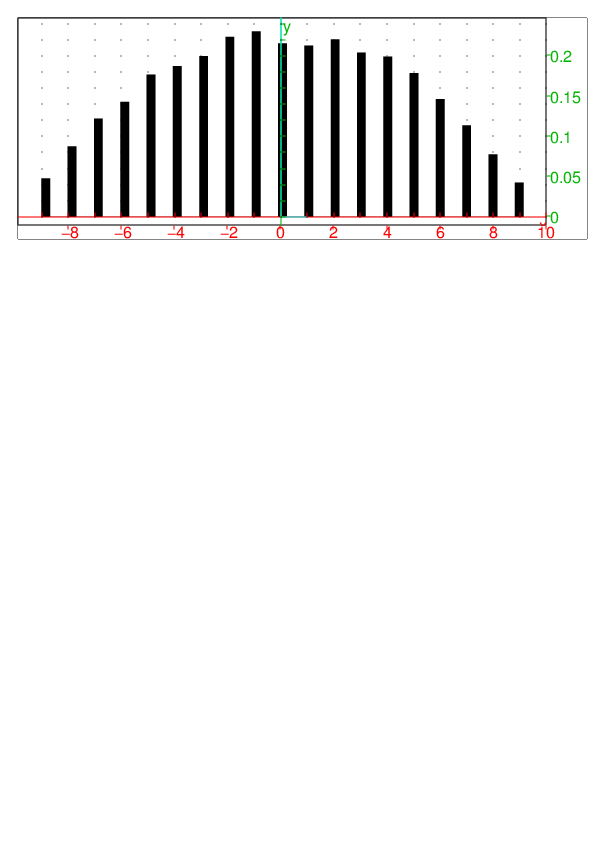
\includegraphics[width=0.75\textwidth]{random_hist1.png}
\end{center}
Input :
\begin{center}
  \tt X:=randvar([3,1,2,5],[alpha,beta,gamma,delta]):;\\randmatrix(5,4,X)
\end{center}
Output :
\[ \begin{vmatrix}\alpha&\beta&\delta&\delta\\ \delta&\alpha&\alpha&\alpha\\ \delta&\gamma&\alpha&\delta\\
\delta&\alpha&\delta&\alpha\\ \alpha&\beta&\delta&\delta\end{vmatrix}\]
Discrete random variables can be used to approximate custom continuous random variables. For example, consider a probability density function $f$ as a mixture of two normal distributions on the support $S=[-10,10]$. We sample $f$ in $N=10000$ points in $S$. Input :
\begin{center}
  \tt F:=normald(3,2,x)+normald(-5,1,x):; c:=integrate(F,x=-10..10):;\\
  f:=unapply(1/c*F,x):;\\
  X:=randvar(f,range=-10..10,10000):;
\end{center}
Now we generate 25000 values of $X$ and plot a histogram :
\begin{center}
  \tt R:=sample(X,25000):;\\
  hist:=histogram(R,-10,0.1):;\\
  PDF:=plot(f(x),display=red+line\_width\_2):;
  hist,PDF
\end{center}
Output :
\begin{center}
  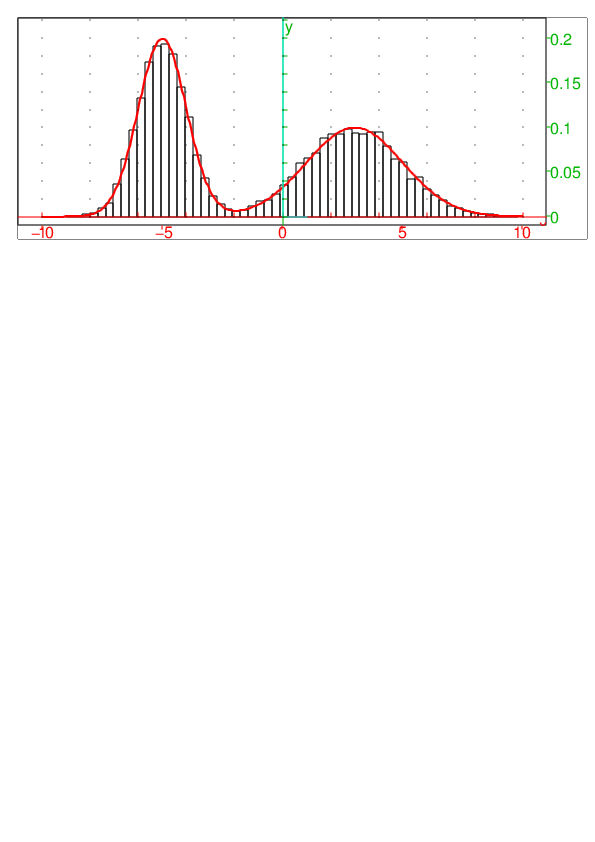
\includegraphics[width=0.75\textwidth]{random_hist2.png}
\end{center}
Sampling from discrete distributions is fast : generating 25 million samples from the distribution of X which
has about 10000 outcomes takes only couple of seconds. In fact, the sampling complexity is constant.
Also observe that the process isn't slowed down by spreading it across 1000 calls of randvector. Input :
\begin{center}
  \tt for k from 1 to 1000 do randvector(25000,X); od:;
\end{center}
{\tt Evaluation time: 2.12}

Independent random variables can be combined in an expression, yielding a new random variable.
In the example below, we define a log-normally distributed variable Y from a variable X with standard
normal distribution. Input :
\begin{center}
  \tt X:=randvar(normal):; mu,sigma:=1.0,0.5:;\\Y:=exp(mu+sigma*X):;\\L:=randvector(10000,Y):; histogram(L,0,0.33)
\end{center}
Output :
\begin{center}
  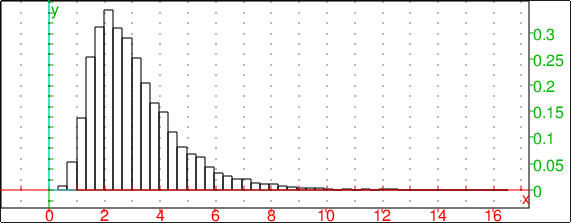
\includegraphics[width=0.75\textwidth]{random_hist3.png}
\end{center}
It is known that $E[Y]=\mathrm{e}^{\mu+\sigma^2/2}$. The mean of $L$ should be close to that number. Input :
\begin{center}
  \tt mean(L); exp(mu+sigma\verb|^|2/2)
\end{center}
Output:
\begin{center}
  \tt 3.0789,3.0802
\end{center}

In case a compound random variable is defined as an expression containing several independent random variables $X,Y,\dots$ of the same type, it is sometimes needed to prevent its evaluation when passing it to {\tt randvector} or {\tt randmatrix}. Input :
\begin{center}
  \tt Y:=randvar(normal):;
\end{center}
$X/Y$ is wrapped by eval because otherwise it would automatically reduce to 1 as $X$ and $Y$ are both {\tt normald}$(0,1)$. Input :
\begin{center}
  \tt randvector(5,eval(X/Y,0))
\end{center}
Output :
\begin{center}
  \tt [0.2608,-0.056913,-4.7966,-1.2622,-1.2997]
\end{center}
To save typing, one can define Z with {\tt eval}$(\ast,0)$ and pass {\tt eval}$(Z,1)$ to {\tt randvector} or {\tt randmatrix}. Input :
\begin{center}
  \tt Z:=eval(X/Y,0):; randvector(5,eval(Z,1))
\end{center}
Output :
\begin{center}
  \tt [0.19015,-2.4509,-1.4277,-1.1452,1.2935]
\end{center}
Parameters of a distribution can be entered as symbols to allow (re)assigning them at any time. Input :
\begin{center}
  \tt purge(lambda):; X:=randvar(exp,lambda):;\\lambda:=1:;
\end{center}
Now execute the following command line several times in a row. The parameter $\lambda$ is updated in each iteration :
\begin{center}
  \tt r:=rand(X); lambda:=sqrt(r)
\end{center}
Output (by executing the above command line three times) :
\begin{center}
  \tt 8.5682,2.9272\\1.5702,1.2531\\0.53244,0.72968
\end{center}

\section{Density and distribution functions}

\subsection{The binomial distribution}

\subsubsection{The probability density function for the binomial
distribution : \texttt{binomial}\index{binomial}}

If you perform an experiment $n$ times, where the probability of
success each time is $p$, then the probability of exactly $k$
successes is 
\[ \texttt{binomial($n$,$k$,$p$)} = \left(^n_k\right) p^k (1-p)^{n-k}\]
This determines the binomial distribution, and so this is called the 
\texttt{binomial} command.  If you enter
\begin{center}
  \tt
  binomial(10,2,0.4)
\end{center}
you will get
\begin{center}
  \tt
  0.120932352
\end{center}
If no third argument $p$ is given, then \texttt{binomial} will just
compute $\left(^n_k\right)$, which recall is called the binomial
coefficient and is also computed by \texttt{comb}.  If you enter
\begin{center}
  \tt
  binomial(10,2)
\end{center}
or
\begin{center}
  \tt
  comb(10,2)
\end{center}
then you will get
\begin{center}
  \tt
   45
\end{center}

\subsubsection{The cumulative distribution function for the binomial
distribution: \texttt{binomial\_cdf}\index{binomial\_cdf}}

Recall that the cumulative distribution function (cdf) for a
distribution is $cdf(x) = \text{Prob}(X \le x)$.  For the binomial
distribution, this is given by the \texttt{binomial\_cdf} command; 
\texttt{binomial\_cdf($n$,$p$,$x$)}, which in this case will equal
\texttt{binomial($n$,$0$,$p$) + \ldots + binomial($n$,floor($x$,$p$)}.
If you enter
\begin{center}
  \tt
  binomial\_cdf(4,0.5,2)
\end{center}
you will get
\begin{center}
  \tt
  0.6875
\end{center}
You can give \texttt{binomial\_cdf} an additional argument;
\texttt{binomial\_cdf($n$,$p$,$x$,$y$) = Prob($x \le X \le y$)}, which
in this case would be
\texttt{binomial($n$,ceil($x$),$p$) + $\cdots$ + binomial($n$,floor($y$),$p$)}.
If you enter
\begin{center}
  \tt
  binomial\_cdf(2,0.3,1,2)
\end{center}
you will get
\begin{center}
  \tt
  0.51
\end{center}

\subsubsection{The inverse distribution function for the binomial
distribution: \texttt{binomial\_icdf}\index{binomial\_icdf}}

Given a value $h$, the inverse distribution function gives the value
of $x$ so that Prob($X \le x$) = $h$; or for discrete distributions,
the smallest $x$ so that Prob($X \le x$) $\ge h$.  For the binomial
distribution with $n$ and $p$, the \texttt{binomial\_icdf} gives the
inverse distribution function.  If you enter
\begin{center}
  \tt
  binomial\_icdf(4,0.5,0.9)
\end{center}
you will get
\begin{center}
  \tt
  3
\end{center}
Note that \texttt{binomial\_cdf(4,0.5,3)}
is $0.9375$, bigger than $0.9$, while 
\texttt{binomial\_cdf(4,0.5,2)} is $0.6875$, smaller than $0.9$.

\subsection{The negative binomial distribution}

\subsubsection{The probability density function for the negative
binomial distribution: \texttt{negbinomial}\index{negbinomial}}
If you repeatedly perform an experiment with probability of success
$p$, then, given an integer $n$, the probability of $k$ failures that occur
before you have $n$ successes is given by the negative binomial
distribution, and can be computed with
\texttt{negbinomial($n$,$k$,$p$)}.  It is given by the formula
$\left(^{n+k-1}_{k}\right)p^n(1-p)^k$.  If you enter
\begin{center}
  \tt
  negbinomial(4,2,0.5)
\end{center}
you will get
\begin{center}
  \tt
  0.15625
\end{center}

Note that
\[
\left(^{n}_{k}\right) = \frac{n!}{k! (n-k)!} = \frac{n (n-1 ) \dots (
n-k+1)}{k!}
\]
The second formula makes sense even if $n$ is negative, and you can
write
\texttt{negbinomial}$(n,k,p) = \left(^{-n}_{k}\right)p^n (p-1)^k$, from
which the name negative binomial distribution comes from.  This also
makes it simple to determine the mean ($n(1-p)/p$) and variance
($n(1-p)/p^2$).  The negative binomial is also called the Pascal
distribution (after Blaise Pascal) or the P\'{o}lya distribution
(after George P\'{o}lya).

\subsubsection{The cumulative distribution function for the negative
binomial distribution: \texttt{negbinomial\_cdf}\index{negbinomial\_cdf}}

The cumulative distribution function for the negative binomial
distribution is given by the \texttt{negbinomial\_cdf} command.  Given
parameters $n$ and $p$, as above, then
\texttt{negbinomial\_cdf($n$,$p$,$x$) = Prob($X \le x$) =
negbinomial($n$,$0$,$p$) + \ldots + negbinomial($n$,floor($x$),$p$)},
and
\texttt{negbinomial\_cdf($n$,$p$,$x$,$y$) = Prob($x \le X \le y$) = 
negbinomial($n$,ceil($x$),$p$) + $\cdots$ + negbinomial($n$,floor($y$),$p$)}.
If you enter
\begin{center}
  \tt
  negbinomial\_cdf(4,0.5,2)
\end{center}
for example, you will get
\begin{center}
  \tt
  0.34375  
\end{center}

\subsubsection{The inverse distribution function for the negative
binomial distribution: \texttt{negbinomial\_icdf}\index{negbinomial\_icdf}}

Given a value $h$, the inverse distribution function gives
the smallest value
of $x$ so that Prob($X \le x$) $\ge h$.
The \texttt{negbinomial\_icdf} gives the inverse
distribution function for the negative binomial distribution.  
If you enter
\begin{center}
  \tt
  negbinomial\_icdf(4,0.5,0.9)
\end{center}
for example, you will get
\begin{center}
  \tt
  8
\end{center}

\subsection{The multinomial probability function: \texttt{multinomial}\index{multinomial}}

If $X$ follows a multinomial probability distribution with
$P = [p_0,p_1,\dots,p_j]$ (where $p_0 + \dots + p_j = 1$),
then for $K=[k_0,\dots,k_j]$ with $k_0 + \dots + k_j = n$, the
probability that $X=K$ is given by the \texttt{multinomial} command; 
\[\texttt{multinomial}(n,P,K)= \frac{n!}{k_0!k_1!\dots
k_j!}(p_0^{k_0}p_1^{k_1}\dots p_j^{k_j}.\]
You will get an error if $k_0 + \dots + k_j$ is not equal to $n$,
although you won't get one if $p_0 + \dots + p_j$ is not equal to $1$.

For example, if you make $10$ choices, where each choice is one of
three items; the first has a $0.2$ probability of being chosen, the
second a $0.3$ probability and the third a $0.5$ probability, the
probability that you end up with $3$ of the first item, $2$ of the
second and $5$ of the third will be
\begin{center}
  \tt
  multinomial(10,[0.2,0.3,0.5],[3,2,5])
\end{center}
or
\begin{center}
  \tt
  0.0567
\end{center}

\subsection{The Poisson distribution}
\subsubsection{The probability density function for the Poisson
distribution: \texttt{poisson}\index{poisson}}

Recall that for the Poisson distribution with parameter $\mu$, the
probability of a non-negative integer $k$ is $e^{-\mu}\mu^k/k!$.  It
will mean $\mu$ and variance $\mu$.  The \texttt{poisson} command will
find this value, given $\mu$ and $k$.  For example,
\begin{center}
  \tt
  poisson(10.0,9)
\end{center}
is
\begin{center}
  \tt
  0.125110035721
\end{center}

\subsubsection{The cumulative distribution function for the Poisson
distribution: \texttt{poisson\_cdf}\index{poisson\_cdf}}

The cumulative distribution function for the Poisson distribution is
given by the \texttt{poisson\_cdf} command with arguments $\mu$ and
$x$; \texttt{poisson\_cdf($\mu$,$x$) = Prob($X \le x$)}.  If you enter
\begin{center}
  \tt
  poisson\_cdf(10.0,3)
\end{center}
you will get
\begin{center}
  \tt
  0.0103360506759
\end{center}

With another argument, \texttt{poisson\_cdf} will find the probability
of falling between two values;
\texttt{poisson\_cdf($\mu$,$x$,$y$) = Prob($x \le X \le y$)}.
If you enter
\begin{center}
  \tt
  poisson\_cdf(10.0,3,10)
\end{center}
you will get
\begin{center}
  \tt
  0.580270354477
\end{center}

\subsubsection{The inverse distribution function for the Poisson
distribution: \texttt{poisson\_icdf}\index{poisson\_icdf}}
Given a value $h$, the inverse distribution function gives
the smallest value
of $x$ so that Prob($X \le x$) $\ge h$.
Given arguments of a parameter $\mu$ and a value $x$, the
\texttt{poisson\_icdf} gives the inverse
distribution function for the poisson distribution.  If you enter
\begin{center}
  \tt
  poisson\_icdf(10.0,0.975)
\end{center}
you will get
\begin{center}
  \tt
  17
\end{center}

\subsection{Normal distributions}
\subsubsection{The probability density function for a normal
distribution: \texttt{normald}\index{normald} \texttt{loi\_normal}\index{loi\_normal}}

The \texttt{normald} (or \texttt{loi\_normal}) command returns the
value of the normal probability density function.  You can give it
arguments of the mean $\mu$, standard deviation $\sigma$ and a value
$x$ then 
\[
\texttt{normald}(\mu,\sigma,x) = \frac{1}{\sqrt{2\pi} \sigma}
e^{(x-\mu)^2/2}
\]
If you enter
\begin{center}
  \tt
  normald(2,1,3)
\end{center}
you will get
\begin{center}
  \tt
  exp(-1/2)/sqrt(2*pi)
\end{center}

If you don't give the command values for $\mu$ and $\sigma$, then
\texttt{normald} will use the values $\mu=0$ and $\sigma = 1$, and so
compute the standard normal density function.  If you enter
\begin{center}
  \tt
  normald(2)
\end{center}
you will get
\begin{center}
  \tt
  1/(sqrt(2*pi)*exp(2))
\end{center}

\subsubsection{The cumulative distribution function for normal
distributions: \texttt{normal\_cdf}\index{normal\_cdf} \texttt{normald\_cdf}\index{normald\_cdf}}

The command \texttt{normal\_cdf} (or \texttt{normald\_cdf}) computes
the cumulative distribution function for the normal distribution.
Like \texttt{normald}, you can give it the mean and standard deviation
of the distribution; if you enter
\begin{center}
  \tt
  normal\_cdf(1,2,1.96)
\end{center}
you will get
\begin{center}
  \tt
  0.684386303484
\end{center}
You can also leave off the mean and standard deviation, in which case
\texttt{normal\_cdf} will compute the cumulative distribution function
for the standard normal distribution;
\begin{center}
  \tt
  normal\_cdf(1,2.1,1.2)
\end{center}
you will get
\begin{center}
  \tt
  0.537937144066
\end{center}

If you give \texttt{normal\_cdf} an extra argument (with or without
the mean and standard deviation), you will get the probability that
the random variable lies between two values;
$\texttt{normal\_cdf($x$,$y$)} = \text{Prob}(x \le X \le y)$.  If you
enter
\begin{center}
  \tt
  normal\_cdf(1,2.1,1.2,9)
\end{center}
you will get
\begin{center}
  \tt
  0.461993238584
\end{center}

\subsubsection{The inverse distribution function for normal
distributions: \texttt{normal\_icdf}\index{normal\_icdf} \texttt{normald\_icdf}\index{normald\_icdf}}
Given a value $h$, the inverse distribution function gives
the value of $x$ with Prob($X \le x$) $\le h$.
The \texttt{normal\_icdf} (or \texttt{normald\_icdf}) will compute the
inverse distribution for the normal distribution.  If no
mean or standard deviation are given, the standard normal distribution
will be used.  If you enter
\begin{center}
  \tt
  normal\_icdf(0.975)
\end{center}
you will get
\begin{center}
  \tt
  1.95996398454
\end{center}
You can, of course, also give the mean and standard deviation.  If you
enter
\begin{center}
  \tt
  normal\_icdf(1,2,0.495)
\end{center}
you will get
\begin{center}
  \tt
  0.974933060984
\end{center}

\subsubsection{The upper tail cumulative function for normal
distributions: \texttt{UTPN}\index{UTPN}}

The \texttt{UTPN} (the Upper Tail Probability - Normal distribution) will compute
$\text{Prob}(X > x)$.  If you don't give it a mean and variance, then
it will compute the probability for the standard normal distribution.
If you enter
\begin{center}
  \tt
  UTPN(1.96)
\end{center}
you will get
\begin{center}
  \tt
  0.0249978951482
\end{center}
You can also specify a mean and a variance, but note that unlike
\texttt{normald} and \texttt{normal\_cdf}, the \texttt{UTPN} requires
the variance and not the standard deviation.  If you enter
\begin{center}
  \tt
  UTPN(1,4,1.96)
\end{center}
you will get
\begin{center}
  \tt
  0.315613696516
\end{center}

\subsection{Student's distribution}

\subsubsection{The probability density function for Student's
distribution: \texttt{student}\index{student} \texttt{studentd}\index{studentd}}

Student's distribution (also called Student's $t$-distribution or just
the $t$-distribution) with
$n$ degrees of freedom has density function given by
\[
\texttt{student}(n,x) =
\frac{\Gamma((n+1)/2)}{\Gamma(n/2)\sqrt{n\pi}}\left(1 +
\frac{x^2}{n}\right)^{-n-1/2}
\]
where recall the Gamma function is defined for $x>0$ by $\Gamma(x) =
\int_0^\infty e^{-t}t^{x-1}dx$.  If you enter
\begin{center}
  \tt
  student(2,3)
\end{center}
you will get
\begin{center}
  \tt
  sqrt(pi)/(11*sqrt(2*pi)*sqrt(11/2))
\end{center}
which can be numerically approximated by
\begin{center}
  \tt
  evalf(student(2,3))
\end{center}
which is
\begin{center}
  \tt
  0.0274101222343
\end{center}

\subsubsection{The cumulative distribution function for Student's
distribution: \texttt{student\_cdf}\index{student\_cdf}}

The cumulative distribution function for Student's distribution with
$n$ degrees of freedom at a value $x$ is
$\texttt{student\_cdf}(n,x) = \texttt{Prob}(X \le x)$; if you
enter
\begin{center}
  \tt
  student\_cdf(5,2)
\end{center}
you will get
\begin{center}
  \tt
  0.949030260585
\end{center}

If you give \texttt{student\_cdf} an extra argument,
you will get the probability that
the random variable lies between two values;
$\texttt{student\_cdf($n$,$x$,$y$)} = \text{Prob}(x \le X \le y)$.  If you
enter
\begin{center}
  \tt
  student\_cdf(5,-2,2)
\end{center}
you will get
\begin{center}
  \tt
  0.89806052117
\end{center}

\subsubsection{The inverse distribution function for Student's
distribution: \texttt{student\_icdf}\index{student\_icdf}}

The inverse distribution function for Student's
distribution with $n$ degrees of freedom is computed with
\texttt{student\_icdf($n$,$h$)}; recall that this will return the
value $x$ with $\texttt{student\_cdf}(n,x) = h$.  If you enter
\begin{center}
  \tt
  student\_icdf(5,0.95)
\end{center}
you will get
\begin{center}
  \tt
  2.01504837333
\end{center}


\subsubsection{The upper tail cumulative function for Student's
distribution: \texttt{UTPT}\index{UTPT}}

The \texttt{UTPT} (the Upper Tail Probability - T distribution) will compute
$\text{Prob}(X > x)$.  
If you enter
\begin{center}
  \tt
  UTPT(5,2)
\end{center}
you will get
\begin{center}
  \tt
  0.0509697394149
\end{center}

\subsection{The $\chi^2$ distribution}

\subsubsection{The probability density function for the $\chi^2$
distribution: \texttt{chisquare}\index{chisquare}}

The $\chi^2$ distribution with
$n$ degrees of freedom has density function given by
\[
\texttt{chisquare}(n,x) =
\frac{x^{n/2-1}e^{-x/2}}{2^{n/2}\Gamma(n/2)}
\]
If you enter
\begin{center}
  \tt
  chisquare(5,2)
\end{center}
you will get
\begin{center}
  \tt
  2*sqrt(2)/(exp(1)*sqrt(2)*3*sqrt(pi))  
\end{center}
which can be numerically approximated by
\begin{center}
  \tt
  evalf(chisquare(5,2))
\end{center}
which is
\begin{center}
  \tt
  0.138369165807
\end{center}

\subsubsection{The cumulative distribution function for the $\chi^2$
distribution: \texttt{chisquare\_cdf}\index{chisquare\_cdf}}

The cumulative distribution function for the $\chi^2$ distribution with
$n$ degrees of freedom at a value $x$ is
$\texttt{chisquare\_cdf}(n,x) = \texttt{Prob}(X \le x)$; if you
enter
\begin{center}
  \tt
  chisquare\_cdf(5,11)
\end{center}
you will get
\begin{center}
  \tt
  0.948620016517
\end{center}

If you give \texttt{chisquare\_cdf} an extra argument,
you will get the probability that
the random variable lies between two values;
$\texttt{chisquare\_cdf($n$,$x$,$y$)} = \text{Prob}(x \le X \le y)$.  If you
enter
\begin{center}
  \tt
  chisquare\_cdf(3,1,2)
\end{center}
you will get
\begin{center}
  \tt
  0.22884525243
\end{center}

\subsubsection{The inverse distribution function for the $\chi^2$
distribution: \texttt{chisquare\_icdf}\index{chisquare\_icdf}}

The inverse distribution function for the $\chi^2$
distribution with $n$ degrees of freedom is computed with
\texttt{chisquare\_icdf($n$,$h$)}; recall that this will return the
value $x$ with $\texttt{chisquare\_cdf}(n,x) = h$.  If you enter
\begin{center}
  \tt
  chisquare\_icdf(5,0.95)
\end{center}
you will get
\begin{center}
  \tt
  11.0704976935
\end{center}

\subsubsection{The upper tail cumulative function for the $\chi^2$
distribution: \texttt{UTPC}\index{UTPC}}

The \texttt{UTPC} (the Upper Tail Probability - Chi-square distribution) will compute
$\text{Prob}(X > x)$.  
If you enter
\begin{center}
  \tt
  UTPC(5,11)
\end{center}
you will get
\begin{center}
  \tt
  0.0513799834831
\end{center}

\subsection{The Fisher-Sn\'{e}d\'{e}cor distribution}

\subsubsection{The probability density function for the Fisher-Sn\'{e}d\'{e}cor distribution: \texttt{fisher}\index{fisher} \texttt{fisherd}\index{fisherd} \texttt{snedecor}\index{snedecor} \texttt{snedecord}\index{snedecord}}

The Fisher-Sn\'{e}d\'{e}cor distribution (also called the F-distribution)
with $n_1$ and $n_2$ degrees of freedom has density function given by
for $x \ge 0$,
\[
\texttt{fisher}(n_1,n_2,x) =
\frac{(n_1/n_2)^{n_1/2}\Gamma((n_1+n_2)/2)}{\Gamma(n_1/2)\Gamma(n_2/2)}
\frac{x^{(n_1-2)/2}}{(1+(n_1/n_2)x)^{(n_1+n_2)/2}}
\]
(The \texttt{snecedor} command is the same as the \texttt{fisher}
command.)
If you enter
\begin{center}
  \tt
  fisher(5,3,2.5)
\end{center}
you will get
\begin{center}
  \tt
  0.10131184472
\end{center}

\subsubsection{The cumulative distribution function  for the Fisher-Sn\'{e}d\'{e}cor distribution: \texttt{fisher\_cdf}\index{fisher\_cdf} \texttt{snedecor\_cdf}\index{snedecor\_cdf}}

The cumulative distribution function for the Fisher-Sn\'{e}d\'{e}cor
distribution with $n_1$ and $n_2$ degrees of freedom at a value $x$ is
$\texttt{fisher\_cdf}(n_1,n_2,x) = \texttt{snedecor}(n_1,n_2,x) =
\texttt{Prob}(X \le x)$; if you enter
\begin{center}
  \tt
  fisher\_cdf(5,3,9)
\end{center}
you will get
\begin{center}
  \tt
  Beta(5/2,3/2,15/16,1)
\end{center}
which can be numerically approximated with
\begin{center}
  \tt
  evalf(fisher\_cdf(5,3,9,10))
\end{center}
which is
\begin{center}
  \tt
  0.949898927032
\end{center}

\subsubsection{The inverse distribution function for the Fisher-Sn\'{e}d\'{e}cor distribution: \texttt{fisher\_icdf}\index{fisher\_icdf} \texttt{snedecor\_icdf}\index{snedecor\_icdf}}

The inverse distribution function for the 
Fisher-Sn\'{e}d\'{e}cor
distribution with $n_1$ and $n_2$ degrees of freedom is computed with
\texttt{fisher\_icdf($n_1$,$n_2$,$h$)}; recall that this will return the
value $x$ with $\texttt{fisher\_cdf}(n_1,n_2,x) = h$.  If you enter
\begin{center}
  \tt
  fisher\_icdf(5,3,0.95)
\end{center}
you will get
\begin{center}
  \tt
  9.01345516752
\end{center}

\subsubsection{The upper tail cumulative function for the Fisher-Sn\'{e}d\'{e}cor distribution: \texttt{UTPF}\index{UTPF}}

The \texttt{UTPF} (the Upper Tail Probability -
Fisher-Sn\'{e}d\'{e}cor distribution) will compute 
$\text{Prob}(X > x)$.  
If you enter
\begin{center}
  \tt
  UTPF(5,3,9)
\end{center}
you will get
\begin{center}
  \tt
  0.050101072968
\end{center}

\subsection{The gamma distribution}
\subsubsection{The probability density function for the gamma distribution: \texttt{gammad}\index{gammad}}

The gamma distribution depends on two parameters, $a>0$ and $b>0$; the
value of the density function at $x \ge 0$ is
$\texttt{gammad}(a,b,x) = x^{a-1}e^{-bx}b^a/\Gamma(a)$.   If you enter
\begin{center}
  \tt
  gammad(2,1,3)
\end{center}
for example, you will get
\begin{center}
  \tt
  3/exp(3)  
\end{center}

\subsubsection{The cumulative distribution function for the gamma distribution: \texttt{gammad\_cdf}\index{gammad\_cdf}}

The cumulative distribution function for the gamma distribution with
parameters $a$ and $b$ at a value $x$ is
$\texttt{gammad\_cdf}(n,x) = \texttt{Prob}(X \le x)$.  It turns out that
$\texttt{gammad\_cdf}(n,x) = \texttt{igamma}(a, bx, 1)$ where
\texttt{igamma} is the incomplete gamma function; 
$\texttt{igamma}(a,x,1) = \int_0^x e^{-t}t^{a-1}dt/\Gamma(a)$.
If you
enter
\begin{center}
  \tt
  gammad\_cdf(2,1,0.5)
\end{center}
you will get
\begin{center}
  \tt
  0.090204010431
\end{center}

If you give \texttt{gammad\_cdf} an extra argument,
you will get the probability that
the random variable lies between two values;
$\texttt{gammad\_cdf($a$,$b$,$x$,$y$)} = \text{Prob}(x \le X \le y)$.  If you
enter
\begin{center}
  \tt
  gammad\_cdf(2,1,0.5,1.5)
\end{center}
you will get
\begin{center}
  \tt
  0.351970589198
\end{center}

\subsubsection{The inverse distribution function for the gamma distribution: \texttt{gammad\_icdf}\index{gammad\_icdf}}

The inverse distribution function for the gamma
distribution with parameters $a$ and $b$ is computed with
\texttt{gammad\_icdf($a$,$b$,$h$)}; recall that this will return the
value $x$ with $\texttt{gammad\_cdf}(a,b,x) = h$.  If you enter
\begin{center}
  \tt
  gammad\_icdf(2,1,0.5)
\end{center}
you will get
\begin{center}
  \tt
  1.67834699002
\end{center}

\subsection{The beta distribution}

\subsubsection{The probability density function for the beta distribution: \texttt{betad}\index{betad}}

The beta distribution depends on two parameters, $a>0$ and $b>0$; the
value of the density function at $x$ in $[0,1]$ is
$\texttt{betad}(a,b,x) =
\Gamma(a+b)x^{a-1}(1-x)^{b-1}/(\Gamma(a)\Gamma(b))$. If you enter
\begin{center}
  \tt
  betad(2,1,0.3)
\end{center}
for example, you will get
\begin{center}
  \tt
  0.6
\end{center}

\subsubsection{The cumulative distribution function for the beta distribution: \texttt{betad\_cdf}\index{betad\_cdf}}

The cumulative distribution function for the beta distribution with
parameters $a$ and $b$ at a value $x$ in $[0,1]$ is
$\texttt{betad\_cdf}(a,b,x) = \texttt{Prob}(X \le x)$.  It turns out
that $\texttt{betad\_cdf}(a,b,x) =
\beta(a,b,x)\Gamma(a+b)/(\Gamma(a)\Gamma(b))$ where
$\beta(a,b,x) = \int_0^x t^{a-1}(1-t)^{b-1} dt$.  
If you
enter
\begin{center}
  \tt
  betad\_cdf(2,3,0.2)
\end{center}
for example, you will get
\begin{center}
  \tt
  0.1808
\end{center}

If you give \texttt{betad\_cdf} an extra argument $y$, also in $[0,1]$,
you will get the probability that
the random variable lies between the two values;
$\texttt{betad\_cdf($a$,$b$,$x$,$y$)} = \text{Prob}(x \le X \le y)$.  
If you enter
\begin{center}
  \tt
  betad\_cdf(2,3,0.25,.5)
\end{center}
you will get
\begin{center}
  \tt
  0.42578125
\end{center}

\subsubsection{The inverse distribution function for the beta distribution: \texttt{betad\_icdf}\index{betad\_icdf}}

The inverse distribution function for the beta
distribution with parameters $a$ and $b$ is computed with
\texttt{betad\_icdf($a$,$b$,$h$)}; recall that this will return the
value $x$ with $\texttt{betad\_cdf}(a,b,x) = h$.  If you enter
\begin{center}
  \tt
  betad\_icdf(2,3,0.2)
\end{center}
you will get
\begin{center}
  \tt
  0.212317128278
\end{center}

\subsection{The geometric distribution}

\subsubsection{The probability density function for the geometric
distribution: \texttt{geometric}\index{geometric}}

If an experiment with probability of success $p$ is iterated, the
probability that the first success occurs on the $k$th trial is
$(1-p)^{k-1}p$.  This gives the geometric distribution (with parameter
$p$) on the natural numbers.  Given such a $p$, the geometric density
function at $n$ is given by $\texttt{geometric}(p,n) = (1-p)^{n-1}p$.
If you enter
\begin{center}
  \tt
  geometric(0.2,3)
\end{center}
for example, you will get
\begin{center}
  \tt
  0.128  
\end{center}

\subsubsection{The cumulative distribution function of the geometric
distribution: \texttt{geometric\_cdf}\index{geometric\_cdf}}

The cumulative distribution function for the geometric distribution with
parameter $p$ at a natural number $n$ is
$\texttt{geometric\_cdf}(p,n) = \texttt{Prob}(X \le n)$, which in this
case turns out to be $\texttt{geometric\_cdf}(p,n) =
1 - (1-p)^n$.
If you enter
\begin{center}
  \tt
  geometric\_cdf(0.2,3)
\end{center}
for example, you will get
\begin{center}
  \tt
  0.488
\end{center}

If you give \texttt{geometric\_cdf} an extra argument $k$, also a
natural number, you will get the probability that
the random variable lies between the two values;
$\texttt{geometric\_cdf($p$,$n$,$k$)} = \text{Prob}(n \le X \le k)$.  
If you enter
\begin{center}
  \tt
  geometric\_cdf(0.2,3,5)
\end{center}
you will get
\begin{center}
  \tt
  0.31232
\end{center}

\subsubsection{The inverse distribution function for the
geometric distribution: \texttt{geometric\_icdf}\index{geometric\_icdf}}

The inverse distribution function for the geometric
distribution with parameter $p$ is computed with
\texttt{geometric\_icdf($p$,$h$)}; recall that this will return the
smallest natural number $n$ with $\texttt{geometric\_cdf}(p,n) \ge  h$.  If you enter
\begin{center}
  \tt
  geometric\_icdf(0.2,0.5)
\end{center}
you will get
\begin{center}
  \tt
  4
\end{center}

\subsection{The Cauchy distribution}

\subsubsection{The probability density function for the Cauchy
distribution: \texttt{cauchy}\index{cauchy} \texttt{cauchyd}\index{cauchyd}}

The probability density function of the Cauchy distribution (sometimes
called the Lorentz distribution) is given by the
\texttt{cauchy} (or \texttt{cauchyd}) command.  The Cauchy
distribution depends on two parameters $a$ and $b$, and the value of
the density function at $x$ is 
$\texttt{cauchy}(a,b,x) = b/(\pi ((x-a)^2 + b^2))$.
If you enter 
\begin{center}
  \tt
  cauchy(2.2,1.5,0.8)
\end{center}
you will get
\begin{center}
  \tt
  0.113412073462
\end{center}

If you leave out the parameters $a$ and $b$, they will default to $0$
and $1$, respectively; $\texttt{cauchy}(x) = 1/(\pi (x^2 + 1))$.  If
you enter
\begin{center}
  \tt
  cauchy(0.3)
\end{center}
you will get
\begin{center}
  \tt
  0.292027418517
\end{center}

\subsubsection{The cumulative distribution function for the Cauchy
distribution: \texttt{cauchy\_cdf}\index{cauchy\_cdf} \texttt{cauchyd\_cdf}\index{cauchyd\_cdf}}

The command \texttt{cauchy\_cdf} (or \texttt{cauchyd\_cdf}) computes
the cumulative distribution function for the Cauchy distribution.
Like \texttt{cauchy}, you can give it the parameters $a$ and $b$, or
let them default to $0$ and $1$.  The Cauchy cumulative distribution
function is given by the formula
$\texttt{cauchy\_cdf}(a,b,x) = 1/2 + \arctan((x-a)/b)/\pi$.
If you enter
\begin{center}
  \tt
  cauchy\_cdf(2,3,1.4)
\end{center}
you will get
\begin{center}
  \tt
  0.437167041811
\end{center}
and if you enter
\begin{center}
  \tt
  cauchy\_cdf(1.4)
\end{center}
you will get
\begin{center}
  \tt
  0.802568456711
\end{center}

If you give \texttt{cauchy\_cdf} an extra argument (with or without
the parameters), you will get the probability that
the random variable lies between two values;
$\texttt{cauchy\_cdf($a$,$b$,$x$,$y$)} = \text{Prob}(x \le X \le y)$.  If you
enter
\begin{center}
  \tt
  cauchy\_cdf(2,3,-1.9,1.4)
\end{center}
you will get
\begin{center}
  \tt
  0.228452641651
\end{center}

\subsubsection{The inverse distribution function for the
Cauchy distribution: \texttt{cauchy\_icdf}\index{cauchy\_icdf} \texttt{cauchyd\_icdf}\index{cauchyd\_icdf}}

Given a value $h$, the inverse distribution function gives
the value of $x$ with $\texttt{Prob}(X \le x) = h$.
The \texttt{cauchy\_icdf} will compute the
inverse distribution for the Cauchy distribution.  (If no
parameters are given, they will be assumed to be 0 and 1.)
If you enter
\begin{center}
  \tt
  cauchy\_icdf(2,3,0.23)
\end{center}
you will get
\begin{center}
  \tt
  -1.40283204777
\end{center}

\subsection{The uniform distribution}
\subsubsection{The probability density function for the uniform
distribution: \texttt{uniform}\index{uniform} \texttt{uniformd}\index{uniformd}}

Given two values $a$ and $b$ with $a < b$, the uniform distribution on
$[a,b]$ has density function $1/(b-a)$ for $x$ in $[a,b]$.  The 
\texttt{uniform} (or \texttt{uniformd}) command will compute this;
$\texttt{uniform}(a,b,x) = 1/(b-a)$.  If you enter
\begin{center}
  \tt
  uniform(2.2,3.5,2.8)
\end{center}
you will get
\begin{center}
  \tt
  0.769230769231
\end{center}

\subsubsection{The cumulative distribution function for the uniform
distribution: \texttt{uniform\_cdf}\index{uniform\_cdf} \texttt{uniformd\_cdf}\index{uniformd\_cdf}}

Given two values $a$ and $b$ with $a <b$, the cumulative distribution
function for the uniform distribution on $[a,b]$ is (for $x$ in $[a,b]$)
$\texttt{uniform\_cdf}(a,b,x) = \texttt{Prob}(X \le x) = (x-a)/(b-a)$.
If you enter
\begin{center}
  \tt
  uniform\_cdf(2,4,3.2)
\end{center}
you will get
\begin{center}
  \tt
  0.6
\end{center}

With an extra argument $y$ in $[a,b]$, \texttt{uniform\_cdf} will
compute $\texttt{uniform\_cdf}(a,b,x,y) = \texttt{Prob}(x \le X \le y)
= (y-x)/(b-a)$.  If you enter
\begin{center}
  \tt
  uniform\_cdf(2,4,3,3.2)
\end{center}
you will get
\begin{center}
  \tt
  0.1
\end{center}

\subsubsection{The inverse distribution function for the
uniform distribution: \texttt{uniform\_icdf}\index{uniform\_icdf} \texttt{uniformd\_icdf}\index{uniformd\_icdf}}

Given a value $h$, the inverse distribution function for a uniform
distribution is the value of $x$ with $\texttt{Prob}(X \le x) =
\texttt{uniform\_cdf}(a,b,x) = h$.  This value is computed with the 
\texttt{uniform\_icdf} command.  If you enter
\begin{center}
  \tt
  uniform\_icdf(2,3,.6)
\end{center}
you will get
\begin{center}
  \tt
  2.6
\end{center}

\subsection{The exponential distribution}

\subsubsection{The probability density function for the exponential distribution: \texttt{exponential}\index{exponential} \texttt{exponentiald}\index{exponentiald}}

The exponential distribution depends on one parameters, $\lambda>0$; the
value of the density function at $x \ge 0$ is
$\texttt{exponential}(\lambda,x) =
\lambda e^{-\lambda x}$.  If you enter
\begin{center}
  \tt
  exponential(2.1,3.5)
\end{center}
for example, you will get
\begin{center}
  \tt
  0.00134944395675
\end{center}

\subsubsection{The cumulative distribution function for the exponential distribution: \texttt{exponential\_cdf}\index{exponential\_cdf} \texttt{exponentiald\_cdf}\index{exponentiald\_cdf}}

The cumulative distribution function for the exponential distribution with
parameter $\lambda > 0$  at a value $x \ge 0$  is
$\texttt{exponential\_cdf}(\lambda,x) = \texttt{Prob}(X \le x)$.
If you enter
\begin{center}
  \tt
  exponential\_cdf(2.3,3.2)
\end{center}
for example, you will get
\begin{center}
  \tt
  0.99936380154
\end{center}

If you give \texttt{exponential\_cdf} an extra argument $y > x$,
you will get the probability that
the random variable lies between the two values;
$\texttt{exponential\_cdf($\lambda$,$x$,$y$)} = \text{Prob}(x \le X \le y)$.  
If you enter
\begin{center}
  \tt
  exponential\_cdf(2.3,0.9,3.2)
\end{center}
you will get
\begin{center}
  \tt
  0.125549583246
\end{center}

\subsubsection{The inverse distribution function for the exponential distribution: \texttt{exponential\_icdf}\index{exponential\_icdf} \texttt{exponentiald\_icdf}\index{exponentiald\_icdf}}

The inverse distribution function for the exponential
distribution with parameter $\lambda > 0$ is computed with
\texttt{exponential\_icdf($\lambda$,$h$)}; recall that this will return the
value $x$ with $\texttt{exponential\_cdf}(\lambda,x) = h$.  If you enter
\begin{center}
  \tt
  exponential\_icdf(2.3,0.87)
\end{center}
you will get
\begin{center}
  \tt
  0.887052534142
\end{center}

\subsection{The Weibull distribution}
\subsubsection{The probability density function for the Weibull
distribution: \texttt{weibull}\index{weibull}
\texttt{weibulld}\index{weibulld}}

The Weibull distribution depends on three parameters; $k>0$, $\lambda
> 0$ and a real number $\theta$.  The probability density at $x$ is
given by $\frac{k}{\lambda}(\frac{x - \theta}{\lambda})^2
e^{-((x-\theta)\lambda)^2}$.  The \texttt{weibull} (or
\texttt{weibulld}) command computes this, where it can take arguments
$k$,$\lambda$,$\theta$ and $x$, where the $\theta$ can be left out and
will default to 0. If you enter
\begin{center}
  \tt
  weibull(2,1,3)
\end{center}
or
\begin{center}
  \tt
  weibull(2,1,0,3)
\end{center}
you will get
\begin{center}
  \tt
  6/exp(9)
\end{center}

\subsubsection{The cumulative distribution function for the Weibull distribution: \texttt{weibull\_cdf}\index{weibull\_cdf} \texttt{weibulld\_cdf}\index{weibulld\_cdf}}

The command \texttt{weibull\_cdf} computes
the cumulative distribution function for the Weibull distribution.
Like \texttt{weibull}, it takes parameters $k$, $\lambda$ and
$\theta$, where $\theta$ will default to 1 if it is omitted.
The Weibull cumulative distribution
function is given by the formula
$\texttt{weibull\_cdf}(k,\lambda,\theta,x) = 1 -
e^{-((x-\theta)/\lambda)^2}$.
If you enter
\begin{center}
  \tt
  weibull\_cdf(2,3,5)
\end{center}
or
\begin{center}
  \tt
  weibull\_cdf(2,3,0,5)
\end{center}
you will get
\begin{center}
  \tt
  1-exp(-25/9)
\end{center}
and if you enter
\begin{center}
  \tt
  weibull\_cdf(2.2,1.5,0.4,1.9)
\end{center}
you will get
\begin{center}
  \tt
  0.632120558829
\end{center}

If you give \texttt{weibull\_cdf} an extra argument (which will
require that $\theta$ be explicitly included), you will get the probability that
the random variable lies between two values;
$\texttt{weibull\_cdf($k$,$\lambda$,$\theta$,$x$,$y$)} = \text{Prob}(x \le X \le y)$.  If you
enter
\begin{center}
  \tt
  weibull\_cdf(2.2,1.5,0.4,1.2,1.9)
\end{center}
for example you will get
\begin{center}
  \tt
  0.410267239944
\end{center}

\subsubsection{The inverse distribution function for the Weibull distribution: \texttt{weibull\_icdf}\index{weibull\_icdf} \texttt{weibulld\_icdf}\index{weibulld\_icdf}}

Given a value $h$, the inverse distribution function gives
the value of $x$ with $\texttt{Prob}(X \le x) = h$.
The \texttt{weibull\_icdf} command will compute the
inverse distribution for the Weibull distribution.  This uses the
arguments $k$, $\lambda$ and $\theta$ as well as $h$, although
$\theta$ can be omitted and will default to 0.
If you enter
\begin{center}
  \tt
  weibull\_icdf(2.2,1.5,0.4,0.632)
\end{center}
you will get
\begin{center}
  \tt
  1.89977657604
\end{center}

\subsection{The Kolmogorov-Smirnov distribution: \texttt{kolmogorovd}\index{kolmogorovd}}

For real $x$, the \texttt{kolmogorovd} command computes the density
function for the Kolmogorov-Smirnov distribution.  
\[
\texttt{kolmogorovd}(x) = 1 - 2\sum_{k=1}^{\infty} (-1)^{k-1} e^{-k^2 x^2}
\]
If you enter 
\begin{center}
  \tt
  kolmogorovd(1.36)
\end{center}
for example, you will get
\begin{center}
  \tt
  0.950514123245
\end{center}

\subsection{The Wilconon or Mann-Whitney distribution}
\subsection{The Wilconon test polynomial: \texttt{wilcoxonp}\index{wilcoxonp}}

The \texttt{wilcoxonp} command will compute the polynomial for the
Wilcoxon or Mann-Whitney test; it can take one or two parameters.  If
you enter
\begin{center}
  \tt
  wilcoxonp(4)
\end{center}
you will get
\begin{center}
  \tt
  poly1[1/16,1/16,1/16,1/8,1/8,1/8,1/8,1/8,1/16,1/16,1/16]
\end{center}
and if you enter
\begin{center}
  \tt
  wilcoxonp(4,3)
\end{center}
you will get
\begin{center}
  \tt
  poly1[1/35,1/35,2/35,3/35,4/35,4/35,1/7,4/35,4/35,3/35,2/35,1/35,1/35]
\end{center}

\subsubsection{The Wilcoxon/Mann-Whitney statistic: \texttt{wilcoxons}\index{wilcoxons}}

Given two lists, or one list and a real number (a median), the
\texttt{wilcoxons} command will return the Wilcoxon or Mann-Whitney statistic. 
If you enter
\begin{center}
  \tt
  wilcoxons([1,3,4,5,7,8,8,12,15,17],10)
\end{center}
you will get
\begin{center}
  \tt
  18
\end{center}
and if you enter
\begin{center}
  \tt
  wilcoxons([1,3,4,5,7,8,8,12,15,17],[2,6,10,11,13,14,15,18,19,20])
\end{center}
you will get
\begin{center}
  \tt
  128.5
\end{center}

\subsubsection{The Wilcoxon or Mann-Whitney test: \texttt{wilcoxont}}
\index{wilcoxont}

The \texttt{wilcoxont} command will perform the Wilcoxon or
Mann-Whitney test, given two samples or one sample and a number (a
median).  It can additionally take an optional third argument of a
function and an optional fourth argument of a real number.
If you enter
\begin{center}
  \tt
  wilcoxont([1,2,3,4,5,7,8,8,12,15,17],[2,6,10,11,13,14,15,18,19,20])
\end{center}
you will get
\begin{verbatim}
   Mann-Whitney 2-sample test, H0 same Median, H1 <>
   ranksum 93.0, shifted ranksum 27.0
   u1=83 ,u2=27, u=min(u1,u2)=27
   Limit value to reject H0 26
   P-value 9055/176358 (0.0513444244094), alpha=0.05 H0 not rejected 
   1
\end{center}
If you enter
\begin{center}
  \tt
  wilcoxont([1,3,4,5,7,8,8,12,15,17],[2,6,10,11,13,14,15,18,19,20],0.3)
\end{center}
you will get
\begin{verbatim}
   Mann-Whitney 2-sample test, H0 same Median, H1 <>
   ranksum 81.5, shifted ranksum 26.5
   u1=73.5 ,u2=26.5, u=min(u1,u2)=26.5
   Limit value to reject H0 35
   P-value 316/4199 (0.0752560133365), alpha=0.3 H0 rejected
   0
\end{verbatim}
and if you enter
\begin{center}
  \tt
  wilcoxont([1,3,4,5,7,8,8,12,15,17] ,10,`>`,0.05)
\end{center}
you will get
\begin{verbatim}
   Wilcoxon 1-sample test, H0 Median=10, H1 M<>10
   Wilcoxon statistic: 18, p-value: 0.375, confidence level: 0.05
   1
\end{verbatim}

\subsection{Moment generating functions for probability distributions: \texttt{mgf}\index{mgf}}

The \texttt{mgf} command will compute the moment generating function
for a probability distribution (such as normal, binomial, poisson,
beta, gamma).  It takes as arguments the name of the distribution and
any necessary parameters.    To find the moment generating function
for the standard normal distribution, you can enter
\begin{center}
  \tt
  mgf(normald,1,0)
\end{center}
and get
\begin{center}
  \tt
  exp(t)
\end{center}
If you enter
\begin{center}
  \tt
  mgf(binomial,n,p)
\end{center}
you will get
\begin{center}
  \tt
  (1-p+p*exp(t))\^{}n
\end{center}

\subsection{Cumulative distribution functions: \texttt{cdf}\index{cdf}}

The \texttt{cdf} command will take as arguments the name of a
probability distribution, along with any needed parameters, and return
an expression for the cumulative distribution function.  If you enter
\begin{center}
  \tt
  cdf(normald,0,1)
\end{center}
you will get
\begin{center}
  \tt
  (erf(x*sqrt(2)/2)+1)/2  
\end{center}

You can evaluate the cumulative distribution function at a value by
adding the value as an argument; if you enter
\begin{center}
  \tt
  cdf(binomial,10,0.5,4)
\end{center}
you will get
\begin{center}
  \tt
  0.376953125
\end{center}

\subsection{Inverse distribution functions: \texttt{icdf}\index{icdf}}

The \texttt{icdf} command will take as arguments the name of a
probability distribution, along with any needed parameters, and return
an expression for the inverse cumulative distribution function.  This
is typically most useful if you evaluate the inverse cumulative
function at a specific value by adding it as an argument.  If you enter
\begin{center}
  \tt
  icdf(normald,0,0.5,0.975)
\end{center}
you will get
\begin{center}
  \tt
  0.97998199227
\end{center}

\subsection{Kernel density estimation : {\tt kernel\_density\index{kernel\_density}}, {\tt kde\index{kde}}}
{\tt kernel\_density} (alias : {\tt kde}) accepts a list of samples $L=[X_1,X_2,\dots,X_n]$ and optionally a sequence of options. It performs kernel density estimation\footnote{For the details on kernel density estimation and its implementation see~: Artur Gramacki, {\it Nonparametric Kernel Density Estimation and Its Computational Aspects}, Springer, 2018.} (KDE), optionally restricted to an interval $[a,b]$, to obtain an estimate $\hat{f}$ of the (unknown) probability density function $f$ from which the samples are drawn, defined by~:
\begin{equation}\label{eq:kde1}
  \hat{f}(x)=\frac{1}{n\,h}\,\sum_{i=1}^nK\left(\frac{x-X_i}{h}\right),
\end{equation}
where $K$ is the Gaussian kernel $K(u)=\frac{1}{\sqrt{2\,\pi}}\,\exp\left(-\frac{1}{2}\,u^2\right)$ and $h$ is the positive real parameter called the \emph{bandwidth}.

The supported options are listed below.
\begin{itemize}
  \item {\tt output=<type>} or {\tt Output=<type>} : specifies the form of the return value $\hat{f}$, where {\tt <type>} may be
  \begin{itemize}
    \item {\tt exact} : $\hat{f}$ is returned as the sum of Gaussian kernels, i.e.~as the right side of~\eqref{eq:kde1}, which is usable only when the number of samples is relatively small (up to few hundreds),
    \item {\tt piecewise} : $\hat{f}$ is returned as a piecewise expression obtained by the spline interpolation of the specified degree (by default, the interpolation is linear) on the interval $[a,b]$ segmented to the specified number of bins,
    \item {\tt list} (the default) : $\hat{f}$ is returned in discrete form, as a list of values $\hat{f}\left(a+k\,\frac{b-a}{M-1}\right)$ for $k=0,1,\dots,M$, where $M$ is the number of bins.
  \end{itemize}
  \item {\tt bandwidth=<value>} : specifies the bandwidth. {\tt <value>} may be
  \begin{itemize}
    \item a positive real number $h$,
    \item {\tt select} (the default) : bandwidth is selected using a direct plug-in method,
    \item {\tt gauss} or {\tt normal} or {\tt normald} : the Silverman's rule of thumb is used for selecting bandwidth (this method is fast but the results are close to optimal ones only when $f$ is approximately normal).
  \end{itemize}
  \item {\tt bins=<posint>} (by default 100) : the number of bins for simplifying the input data. Only the number if samples in each bin is stored. Bins represent the elements of an equidistant segmentation of the interval $S$ on which KDE is performed. This allows evaluating kernel summations using convolution when {\tt output} is set to {\tt piecewise} or {\tt list}, which significantly lowers the computational burden for large values of $n$ (say, few hundreds or more). If {\tt output} is set to {\tt exact}, this option is ignored.
  \item {\tt [range=]a..b} or {\tt range=[a,b]} or {\tt x=a..b} : the interval $[a,b]$ on which KDE is performed. If an identifier $x$ is specified, it is used as the variable of the output. If the range endpoints are not specified, they are set to $a=\min_{1\leq i\leq n} X_i-3\,h$ and $b=\max_{1\leq i\leq n}X_i+3\,h$ (unless {\tt output} is set to {\tt exact}, in which case this option is ignored).
  \item {\tt interp=<posint>} (by default 1) : the degree of the spline interpolation, ignored unless {\tt output} is set to {\tt piecewise}.
  \item {\tt spline=<posint>} : sets {\tt option} to {\tt piecewise} and {\tt interp} to {\tt <posint>}.
  \item {\tt eval=x0} : only the value $\hat{f}(x_0)$ is returned (this cannot be used with {\tt output} set to {\tt list}).
  \item an unassigned identifier {\tt x} (by default $x$) : the variable of the output.
  \item {\tt exact} : the same as {\tt output=exact}.
  \item {\tt piecewise} : the same as {\tt output=piecewise}.
\end{itemize}

\paragraph{Examples.}
Input :
\begin{center}
  \tt kernel\_density([1,2,3,2],bandwidth=1/4,exact)
\end{center}
Output :
\begin{center}
  \tt 0.4*(exp(-8*(x-3)\verb|^|2)+2*exp(-8*(x-2)\verb|^|2)+exp(-8*(x-1)\verb|^|2))
\end{center}
Input :
\begin{center}
  \tt f:=unapply(normald(4,1,x)/2+normald(7,1/2,x)/2,x); plot(f(x),x=0..10)
\end{center}
Output :
\begin{center}
  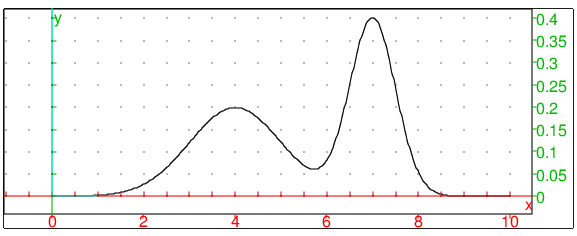
\includegraphics[width=0.75\textwidth]{kde_plot1.png}
\end{center}
Input :
\begin{center}
  \tt X:=randvar(f,range=0..10,1000):; S:=sample(X,1000):; F:=kernel\_density(S,piecewise):; plot([F,f(x)],x=0..10, display=[line\_width\_2+blue,line\_width\_1+black])
\end{center}
Output :
\begin{center}
  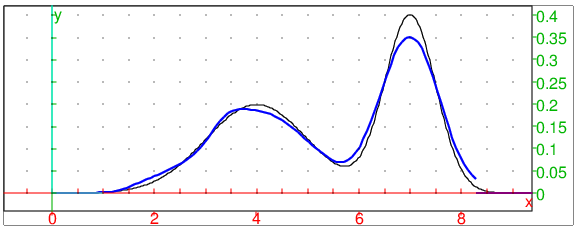
\includegraphics[width=0.75\textwidth]{kde_plot2.png}
\end{center}
Input :
\begin{center}
  \tt kernel\_density(S,bins=50,spline=3,eval=4.75)
\end{center}
Output :
\begin{center}
  \tt 0.14655478136
\end{center}
Input :
\begin{center}
  \tt time(kernel\_density(sample(X,1e5),piecewise))
\end{center}
Output :
\begin{center}
  \tt "Done",[0.17,0.1653323]
\end{center}
Input :
\begin{center}
  \tt S:=sample(X,5000):; sqrt(int((f(x)-kde(S,piecewise))\verb|^|,x=0..10))
\end{center}
Output :
\begin{center}
  \tt 0.0269841239243
\end{center}
Input :
\begin{center}
  \tt S:=sample(X,25000):; sqrt(int((f(x)-kde(S,bins=150,piecewise))\verb|^|2,x=0..10))
\end{center}
Output :
\begin{center}
  \tt 0.0144212781377
\end{center}

\subsection{Distribution fitting by maximum likelihood : {\tt fitdistr\index{fitdistr}}}
{\tt fitdistr} takes two arguments, a list $L$ of presumably independent and identically distributed samples and a distribution type, which may be normal, exponential, Poisson, geometric, gamma, beta, Cauchy or Weibull. The type is specified as {\tt normal} ({\tt normald}), {\tt exp} ({\tt exponential} or {\tt exponentiald}), {\tt poisson}, {\tt geometric}, {\tt gammad}, {\tt betad}, {\tt cauchy} ({\tt cauchyd}) or {\tt weibull} ({\tt weibulld}), respectively. The command returns the distribution of the specified type with parameters that fit the given samples most closely according to the method of maximum likelihood.

For example, input :
\begin{center}
  \tt S:=:; fitdistr(randvector(1000,weibulld,1/2,1),weibull)
\end{center}
Output :
\begin{center}
  \tt weibulld(0.498920254339,0.971148738409)
\end{center}
Input :
\begin{center}
  \tt X:=randvar(normal,stddev=9.5):; Y:=randvar(normal,stddev=1.5):; S:=sample(eval(X/Y,0),1000):; Z:=fitdistr(S,cauchy)
\end{center}
Output :
\begin{center}
  \tt cauchyd(-0.13160176167,6.2569300393)
\end{center}
Input :
\begin{center}
  \tt histogram(select(x->(x>-100 and x<100),S)); plot(Z(x),x=-100..100,display=red+line\_width\_2)
\end{center}
Output :
\begin{center}
  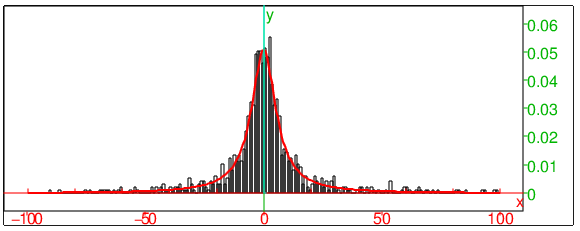
\includegraphics[width=0.75\textwidth]{fitdistr.png}
\end{center}
Input :
\begin{center}
  \tt kolmogorovt(S,Z)
\end{center}
Output :
\begin{center}
  \tt ["D=",0.0125864995943,"K=", 0.398020064869, "1-kolmogorovd(K)=",0.997387219452]
\end{center}
The Kolmogorov-Smirnov test indicates that the samples from $S$ are drawn from $Z$ with high probability.

Fitting a lognormal distribution to samples $x_1,x_2,\dots,x_n$ can be done by fitting a normal distribution to the sample logarithms $\log x_1,\log x_2,\dots,\log x_n$ because log-likelihood functions are the same. For example, generate some samples according to the lognormal rule with parameters $\mu=5$ and $\sigma^2=2$ :
\begin{center}
  \tt X:=randvar(normal,mean=5,variance=2):; S:=sample(exp(X),1000):;
\end{center}
Now fit normal distribution to $\log S$ :
\begin{center}
  \tt Y:=fitdistr(log(S),normal)
\end{center}
Output :
\begin{center}
  \tt normald(5.04754808715,1.42751619912)
\end{center}
The mean of $Y$ is about $5.05$ and the variance is about $2.04$. Now the variable $Z=\exp(Y)$ has the sought lognormal distribution.

\subsection{Markov chains: \texttt{markov}\index{markov}}

Given the transition matrix of a Markov chain, the \texttt{markov}
command will compute characteristic features of the chain.  If $M$ is
a transition matrix, then \texttt{markov($M$)} will return the list of
the positive recurrent states, the list of corresponding
invariant probabilities, the list of other strong connected
components, the list of probabilities of ending up in the sequence of
recurrent states. 
For example, if you enter
\begin{center}
  \tt
  markov([[0,0,1/2,0,1/2],[0,0,1,0,0],[1/4,1/4,0,1/4,1/4],[0,0,1/2,0,1/2],[0,0,0,0,1]])
\end{center}
you will get
\begin{center}
  \tt
  [[4]],[[0,0,0,0,1]],[[3,1,2,0]],[[1],[1],[1],[1],[1]]
\end{center}

\subsection{Generating a random walks: \texttt{randmarkov}\index{randmarkov}}

Given the transition matrix $M$ for a Markov chain and an initial
state $i_0$, the command \texttt{randmarkov($M$,$i_0$,$n$)} will
generate a random walk (given as a vector) starting at $i_0$ and
taking $n$ random steps, where each step is a transition with
probabilities given by $M$.  For example, if you enter
\begin{center}
  \tt
  randmarkov([[0,1/2,0,1/2],[0,1,0,0],[1/4,1/4,1/4,1/4],[0,0,1/2,1/2]],2,10)
\end{center}
you might get
\begin{center}
  \tt
  [2,3,2,0,3,2,2,0,3,2,0]  
\end{center}

Alternatively, given a vector $v = [n_1,\dots,n_p]$, the command
\texttt{randmatrix($v$,$i_0$)} will create a stochastic matrix with
$p$ recurrent loops (given by $v$) and $i_0$ transient states.  If you
enter
\begin{center}
  \tt
  randmarkov([1,2],2)
\end{center}
you might get
\begin{center}
  \tt
   [[1.0,0.0,0.0,0.0,0.0],
    [0.0,0.289031975209,0.710968024791,0.0,0.0],
    [0.0,0.46230383289,0.53769616711,0.0,0.0],
    [0.259262238137,0.149948861946,0.143448150524,0.242132758802,0.205207990592],
    [0.231568633749,0.145429586345,0.155664673778,0.282556511895,0.184780594232]]      
\end{center}

\section{Hypothesis testing}

\subsection{General}

Given a random variable $X$, you may want to know whether some
effective parameter $p$ is the same as some expected value $p_0$.  You
will then want to test the hypothesis $p = p_0$, which will be the
null hypothesis $H_0$.  The alternative hypothesis will be $H_1$.
The tests are:
\begin{description}
   \item[Two-tailed test]  This test will reject the hypothesis $H_0$
   if the relevant statistic is outside of a determined interval.
   This can be denoted '!='.
   \item[Left-tailed test] This test will reject the hypothesis $H_0$
   if the relevant statistic is less than a specific value.
   This can be denoted '<'.
   \item[Right-tailed test] This test will reject the hypothesis $H_0$
   if the relevant statistic is greater than a specific value.
   This can be denoted '>'.
\end{description}

\subsection{Testing the mean with the Z test: \texttt{normalt}\index{normalt}}

The \texttt{normalt} command will use the Z test to test the mean of
data.
You need to provide the command with the following arguments:
\begin{enumerate}
  \item
  The sample data information can be given as a list $[n_s,n_e]$
  consisting of the number of successes $n_s$ and the number of trials
  $n_e$, or a list $[m,t]$ consisting of the mean $m$ and the sample
  size $t$, or a data list of the sample.
  \item
  The mean of the population to or a data list from a control sample.
  \item
  The standard deviation of the population.  If the data list from a
  control sample is provided, then this item is unnecessary.
  \item
  The type of test; "!=","<" or ">".
  \item
  The confidence level.  This is optional; the default
  value is $0.05$.
\end{enumerate}
The \texttt{normalt} command will return the result of a Z test.  It
will return 0 if the test fails, 1 if the test succeeds, and it will
display a summary of the test.

If you enter
\begin{center}
  \tt
  normalt([10,30], 0.5, 0.02, '!=', 0.1)
\end{center}
you will get
\begin{verbatim}
   *** TEST RESULT 0 ***
   Summary Z-Test null hypothesis H0 mu1=mu2, alt. hyp. H1 mu1!=mu2.
   Test returns 0 if probability to observe data is less than 0.1
   (null hyp. mu1=mu2 rejected with less than alpha probability error)
   Test returns 1 otherwise (can not reject null hypothesis)
   Data mean mu1=10, population mean mu2=0.5
   alpha level 0.1, multiplier*stddev/sqrt(sample size)= 1.64485*0.02/5.47723
   0
\end{verbatim}
If you enter
\begin{center}
  \tt
  normalt([0.48,50],0.5,0.1,'<')
\end{center}
you will get
\begin{verbatim}
   *** TEST RESULT 1 ***
   Summary Z-Test null hypothesis H0 mu1=mu2, alt. hyp. H1 mu1<mu2.
   Test returns 0 if probability to observe data is less than 0.05
   (null hyp. mu1=mu2 rejected with less than alpha probability error)
   Test returns 1 otherwise (can not reject null hypothesis)
   Data mean mu1=0.48, population mean mu2=0.5
   alpha level 0.05, multiplier*stddev/sqrt(sample size)= 1.64485*0.1/7.07107
   1
\end{verbatim}

\subsection{Testing the mean with the T test: \texttt{studentt}\index{studentt}}

The \texttt{studentt} command will examine whether data conforms to
Student's distribution.  For small sample sizes, the \texttt{studentt}
test is preferable to \texttt{normalt}.
You need to provide the \texttt{studentt} command with the following
arguments:
\begin{enumerate}
  \item
  The sample data information can be given as a list $[n_s,n_e]$
  consisting of the number of successes $n_s$ and the number of trials
  $n_e$, or a list $[m,t]$ consisting of the mean $m$ and the sample
  size $t$, or a data list of the sample.
  \item
  The mean of the population to or a data list from a control sample.
  \item
  The standard deviation of the population.  If the data list from a
  control sample is provided, then this item is unnecessary.
  \item
  The type of test; "!=","<" or ">".
  \item
  The confidence level.  This is optional; the default
  value is $0.05$.
\end{enumerate}
The \texttt{studentt} command will return the result of a T test.  It
will return 0 if the test fails, 1 if the test succeeds, and it will
display a summary of the test.

If you enter
\begin{center}
  \tt
  studentt([10,20], 0.5, 0.02, '!=', 0.1)
\end{center}
you will get
\begin{verbatim}
   *** TEST RESULT 0 ***
   Summary T-Test null hypothesis H0 mu1=mu2, alt. hyp. H1 mu1!=mu2.
   Test returns 0 if probability to observe data is less than 0.1
   (null hyp. mu1=mu2 rejected with less than alpha probability error)
   Test returns 1 otherwise (can not reject null hypothesis)
   Data mean mu1=10, population mean mu2=0.5, degrees of freedom 20
   alpha level 0.1, multiplier*stddev/sqrt(sample size)= 1.32534*0.02/4.47214
   0
\end{verbatim}
If you enter
\begin{center}
  \tt
  studentt([0.48,20],0.5,0.1,'<')
\end{center}
you will get
\begin{verbatim}
   *** TEST RESULT 1 ***
   Summary T-Test null hypothesis H0 mu1=mu2, alt. hyp. H1 mu1<mu2.
   Test returns 0 if probability to observe data is less than 0.05
   (null hyp. mu1=mu2 rejected with less than alpha probability error)
   Test returns 1 otherwise (can not reject null hypothesis)
   Data mean mu1=0.48, population mean mu2=0.5, degrees of freedom 20
   alpha level 0.05, multiplier*stddev/sqrt(sample size)= 1.72472*0.1/4.47214
   1
\end{verbatim}

\subsection{Testing a distribution with the $\chi^2$ distribution: \texttt{chisquaret}\index{chisquaret}}

The \texttt{chisquaret} command will use the $\chi^2$ test to compare
sample data to a specified distribution.
You need to provide \texttt{chisquaret} with the following arguments:
\begin{enumerate}
  \item A list of sample data.
  \item The name of a distribution, or another list of sample data.
  If this is omitted, a uniform distribution will be used.
  \item The parameters of the distribution, if a name is given as the
  previous argument, or the parameter \texttt{class} followed by
  \texttt{class\_min} and \texttt{class\_dim} (or the default values
  will be used).
\end{enumerate}
The \texttt{chisquaret} command will return the result of the $\chi^2$
test between the sample data and the named distribution or the two
sample data.

For example, if you enter
\begin{center}
  \tt
  chisquaret([57,54])
\end{center}
you will get
\begin{verbatim}
  Guessing data is the list of number of elements in each class, 
           adequation to uniform distribution
  Sample adequation to a finite discrete probability distribution
  Chi2 test result 0.0810810810811,
  reject adequation if superior to chisquare_icdf(1,0.95)=3.84145882069 or chisquare_icdf(1,1-alpha) if alpha!=5%
  0.0810810810811
\end{verbatim}
If you enter
\begin{center}
  \tt
  chisquaret([1,1,1,1,1,0,0,1,0,1,1],[.4,.6])
\end{center}
you will get
\begin{verbatim}
   Sample adequation to a finite discrete probability distribution
   Chi2 test result 0.742424242424,
   reject adequation if superior to chisquare_icdf(1,0.95)=3.84145882069 
                        or chisquare_icdf(1,1-alpha) if alpha!=5%
   0.742424242424
\end{verbatim}
If you enter
\begin{center}
  \tt
  chisquaret(ranv(1000,binomial,10,.5),binomial)
\end{center}
you will get
\begin{verbatim}
   Binomial: estimating n and p from data 10 0.5055
   Sample adequation to binomial(10,0.5055,.), Chi2 test result 7.77825189838,
   reject adequation if superior to chisquare_icdf(7,0.95)=14.0671404493 
                        or chisquare_icdf(7,1-alpha) if alpha!=5%
   7.77825189838
\end{verbatim}
and if you enter
\begin{center}
  \tt
  chisquaret(ranv(1000,binomial,10,.5),binomial,11,.5)
\end{center}
you will get
\begin{verbatim}
   Sample adequation to binomial(11,0.5,.), Chi2 test result 125.617374161,
   reject adequation if superior to chisquare_icdf(10,0.95)=18.3070380533 
                        or chisquare_icdf(10,1-alpha) if alpha!=5%
   125.617374161
\end{verbatim}
For an example using \texttt{class\_min} and \texttt{class\_dim}, let
\begin{center}
  \tt
  L := ranv(1000,normald,0,.2)
\end{center}
If you then enter
\begin{center}
  \tt
  chisquaret(L,normald,classes,-2,.25)
\end{center}
or equivalently set \texttt{class\_min} to $-2$ and
\texttt{class\_dim} to $-0.25$ in the graphical configuration and enter
\begin{center}
  \tt
  chisquaret(L,normald,classes)  
\end{center}
you will get
\begin{verbatim}
   Normal density, 
        estimating mean and stddev from data -0.00345919752912 0.201708100832
   Sample adequation to normald_cdf(-0.00345919752912,0.201708100832,.), 
        Chi2 test result 2.11405080381,
   reject adequation if superior to chisquare_icdf(4,0.95)=9.48772903678
        or chisquare_icdf(4,1-alpha) if alpha!=5%
   2.11405080381
\end{verbatim}
In this last case, you are given the value of $d^2$ of the statistic 
$D^2 = \sum_{j=1}^{k} (n_j - e_j)/e_j$, where $k$ is the number of
sample classes for \texttt{classes(L,-2,0.25)} (or
\texttt{classes(L)}), $n_j$ is the size of the $j$th class, and $e_j =
n p_j$ where $n$ is the size of \texttt{L} and $p_j$ is the
probability of the $j$th class interval assuming a normal distribution
with the mean and population standard deviation of \texttt{L}.

\subsection{Testing a distribution with the Kolmogorov-Smirnov
distribution: \texttt{kolmogorovt}\index{kolmogorovt}}

The \texttt{kolmogorovt} command will use the Kolmogorov test to compare
sample data to a specified continuous distribution.
You need to provide \texttt{kolmogorovt} with either two lists of data
or a list of data followed by the name of a distribution with the
parameters.
The \texttt{kolmogorovt} command will return three values:
\begin{itemize}
  \item The $D$ statistic, which is the maximum distance between the
  cumulative distribution functions of the samples or the sample and
  the given distribution.
  \item The $K$ value, where $K = D\sqrt{n}$ (for a single data set,
  where $n$ is the size of the data set) or $K=D\sqrt{n_1 n_2 /(n_1 +
  n_2)}$ (when there are two data sets, with sizes $n_1$ and $n_2$).
  The $K$ value will tend towards the Kolmogorov-Smirnov distribution
  as the size of the data set goes to infinity.
  \item \texttt{1 - kolmogorovd(K)}, which will be close to 1 when the
  distributions look like they match.
\end{itemize}
For example, if you enter
\begin{center}
  \tt
  kolmogorovt(randvector(100,normald,0,1),normald(0,1))
\end{center}
you might get
\begin{center}
  \tt
  ["D=",0.112592987625,"K=",1.12592987625,"1-kolmogorovd(K)=",0.158375510292]
\end{center}
and if you enter
\begin{center}
  \tt
  kolmogorovt(randvector(100,normald,0,1),student(2))
\end{center}
you might get
\begin{center}
  \tt
  ["D=",0.0996114067923,"K=",0.996114067923,"1-kolmogorovd(K)=",0.27418851907]
\end{center}

\chapter{Numerical computations}\label{sec:numeric}
Real numbers may have an exact representation
(e.g. rationals, symbolic expressions
involving square roots or constants like $\pi$, ...)
or approximate representation, which means that the real
is represented by a rational (with a denominator that is a power
of the basis of the representation) close to the real.
Inside {\tt Xcas}, the standard scientific notation is used
for approximate representation, that is a mantissa (with a point
as decimal separator) optionally followed by the letter {\tt e}
and an integer exponent.

Note that the real number $10^{-4}$ is an exact number but
$1e-4$ is an approximate representation of this number.

\section{Floating point representation.}
In this section, we explain how real numbers are represented.

\subsection{Digits}
The {\tt Digits} variable is used to control how real numbers
are represented and also how they are displayed.
When the specified
number of digits is less or equal to 14 (for example {\tt
  Digits:=14}), then hardware floating point
numbers are used and they are displayed using the specified
number of digits.
When {\tt Digits} is larger than 14, Xcas uses the MPFR
library, the representation is similar to hardware floats
(cf. infra) but the number of bits of
the mantissa is not fixed and the range of exponents is much larger.
More precisely, the number of bits of the mantissa of a created MPFR float
is {\tt ceil(Digits*log(10)/log(2))}.

Note that if you change the value of {\tt Digits}, this will affect
the creation of new real numbers compiled from command lines 
or programs or by instructions like {\tt approx}, but it will
not affect existing real numbers. Hence hardware floats may coexist
with MPFR floats, and even in MPFR floats, some may have 100 bits
of mantissa and some may have 150 bits of mantissa. If operations
mix different kinds of floats, the most precise kind of floats
are coerced to the less precise kind of floats.

\subsection{Representation by hardware floats}
A real is represented by a floating number $d$, that is
\[ d=2^\alpha*(1+m),  \quad 0<m<1, -2^{10} < \alpha < 2^{10} \]
If $\alpha>1-2^{10}$, then $m \geq 1/2$, and $d$ is
a normalized floating point number, otherwise
$d$ is denormalized ($\alpha=1-2^{10}$). The special exponent $2^{10}$
is used to represent plus or minus infinity and NaN (Not a Number).
A hardware float is made of 64 bits:
\begin{itemize}
\item  the first bit is for the sign of $d$ (0 for '+' and 1 for '-')
\item  the 11 following bits represents the exponent, more precisely 
if $\alpha$ denotes the integer from the 11 bits,
the exponent is $\alpha+2^{10}-1$, 
\item  the 52 last bits codes the mantissa $m$, more precisely if
$M$ denotes the integer from the 52 bits, then
$m=1/2+M/2^{53}$ for normalized floats and $m=M/2^{53}$ for
denormalized floats.
\end{itemize}
Examples of representations of the exponent:
\begin{itemize}
\item $\alpha=0$ is coded by 011 1111 1111
\item $\alpha=1$ is coded by 100 0000 0000
\item $\alpha=4$ is coded by 100 0000 0011
\item $\alpha=5$ is coded by 100 0000 0100
\item $\alpha=-1$ is coded by 011 1111 1110
\item $\alpha=-4$ is coded by 011 1111 1011
\item $\alpha=-5$ is coded by 011 1111 1010
\item $\alpha=2^{10}$ is coded by 111 1111 1111
\item $\alpha=2^{-10}-1$ is coded by 000 0000 000
\end{itemize}
{\bf Remark}: $2^{-52}=0.2220446049250313e-15$

\subsection{Examples of representations of normalized floats}
\begin{itemize}
\item 3.1 :\\
We have :
\begin{eqnarray*}
3.1&=&2*(1+\frac{1}{2}+\frac{1}{2^5}+\frac{1}{2^6}+
\frac{1}{2^9}+\frac{1}{2^{10}}+....)\\
&=&2*(1+\frac{1}{2}+\sum_{k=1}^\infty(\frac{1}{2^{4*k+1}}+\frac{1}{2^{4*k+2}}) ) 
\end{eqnarray*}
hence $\alpha=1$ and 
$m=\frac{1}{2}+\sum_{k=1}^\infty(\frac{1}{2^{4*k+1}}+\frac{1}{2^{4*k+2}})$.
Hence the hexadecimal and binary representation of 3.1 is:
\begin{verbatim}
40 (01000000), 8 (00001000), cc (11001100), cc (11001100), 
cc (11001100), cc (11001100), cc (11001100), cd (11001101),
\end{verbatim}
the last octet is 1101, the last bit is 1, because the
following digit is 1 (upper rounding).
\item  3. :\\
We have $3=2*(1+1/2)$.
Hence the hexadecimal and binary representation of 3 is:
\begin{verbatim}
40 (01000000), 8 (00001000), 0 (00000000), 0 (00000000), 
0 (00000000), 0 (00000000), 0 (00000000), 0 (00000000)
\end{verbatim}
\end{itemize}

\subsection{Difference between the representation of (3.1-3) and of 0.1}
\begin{itemize}
\item representation of  0.1 :\\
We have :
\[ 0.1=2^{-4}*(1+\frac{1}{2}+\frac{1}{2^4}+\frac{1}{2^5}+
\frac{1}{2^8}+\frac{1}{2^9}+...)=
2^{-4}*\sum_{k=0}^\infty (\frac{1}{2^{4*k}}+\frac{1}{2^{4*k+1}}) \]
hence $\alpha=1$ and $m=\frac{1}{2}+
\sum_{k=1}^\infty (\frac{1}{2^{4*k}}+\frac{1}{2^{4*k+1}})$,
therefore the representation of 0.1 is
\begin{verbatim}
3f (00111111), b9 (10111001), 99 (10011001), 99 (10011001),
99 (10011001), 99 (10011001), 99 (10011001), 9a (10011010),
\end{verbatim}
the last octet is 1010, indeed the 2 last bits 
01 became 10  because the following digit is 1 (upper rounding).

\item representation of a:=3.1-3 :\\
Computing a is done by adjusting exponents (here nothing
to do), then subtract the mantissa, and adjust the
exponent of the result to have a normalized float.
The exponent is $\alpha=-4$ (that corresponds at $2*2^{-5}$) 
and the bits 
corresponding to the mantissa begin at $1/2=2*2^{-6}$ :
the bits of the mantissa are shifted to the left of 5 positions
and we have :
\begin{verbatim}
3f (00111111), b9 (10111001), 99 (10011001), 99 (10011001),
99 (10011001), 99 (10011001), 99 (10011001), 9a (10100000),
\end{verbatim}
Therefore
$a>0.1$ and  $a-0.1=1/2^{50}+1/2^{51}$ 
(since 100000-11010=110)
\end{itemize}
{\bf Remark}\\
This is the reason why
\begin{center}
{\tt floor(1/(3.1-3))} 
\end{center}
returns {\tt 9} and not {\tt 10} when {\tt Digits:=14}.

\section{Approx. evaluation : {\tt evalf approx} and {\tt Digits}}\index{evalf|textbf}\index{approx|textbf}\index{DIGITS}\index{Digits}
\noindent {\tt evalf} or {\tt approx} evaluates to a numeric
approximation (if possible).\\
Input :
\begin{center}{\tt evalf(sqrt(2))}\end{center}
Output, if in the {\tt cas} configuration ({\tt Cfg} menu) {\tt Digits=7} 
(that is hardware floats are used, and 7 digits are displayed) :
\begin{center}{\tt 1.414214}\end{center}
You can change the number of digits in a command line by assigning 
the variable {\tt DIGITS} or {\tt Digits}.
Input :
\begin{center}{\tt DIGITS:=20}\end{center}
\begin{center}{\tt evalf(sqrt(2))}\end{center}
Output :
\begin{center}{\tt 1.4142135623730950488}\end{center}
Input : 
\begin{center}{\tt evalf(10\verb|^|-5)}\end{center}
Output :
\begin{center}{\tt 1e-05}\end{center}
Input :
\begin{center}{\tt evalf(10\verb|^|15)}\end{center}
Output :
\begin{center}{\tt 1e+15}\end{center}
Input : 
\begin{center}{\tt evalf(sqrt(2))*10\verb|^|-5}\end{center}
Output :
\begin{center}{\tt 1.41421356237e-05}\end{center}

\section{Numerical algorithms}
\subsection{Approximate solution of an equation : {\tt newton}}\index{newton}
\noindent{\tt newton} takes as arguments : an expression {\tt ex}, 
the variable
name of this expression (by default {\tt x}), and three values {\tt a} (by 
default {\tt a=0}), {\tt eps} (by default {\tt eps=1e-8}) and {\tt nbiter} 
(by default {\tt nbiter=12}).\\
{\tt newton(ex,x,a,eps,nbiter)} computes an approximate 
solution {\tt x} of the equation {\tt ex=0}
using the Newton algorithm with starting point 
{\tt x=a}. The maximum number of iterations is {\tt nbiter}
and the precision is {\tt eps}.\\
Input :
\begin{center}{\tt newton(x\verb|^|2-2,x,1) }\end{center}
Output :
\begin{center}{\tt 1.41421356237}\end{center}
Input :
\begin{center}{\tt newton(x\verb|^|2-2,x,-1) }\end{center}
Output :
\begin{center}{\tt -1.41421356237}\end{center}
Input :
\begin{center}{\tt newton(cos(x)-x,x,0)}\end{center}
Output :
\begin{center}{\tt0.739085133215 }\end{center}

\subsection{Approximate computation of the derivative number : {\tt nDeriv}}\index{nDeriv}
\noindent{\tt nDeriv} takes as arguments : an expression {\tt ex}, the variable
name of this expression (by default {\tt x}), and {\tt h} (by default 
{\tt h=0.001}).\\
{\tt nDeriv(ex,x,h)} computes an approximated value of the derivative of the
expression {\tt ex} at the point {\tt x} and returns :
\begin{center}{\tt (f(x+h)-f(x+h))/2*h}\end{center}
Input :
\begin{center}{\tt nDeriv(x\verb|^|2,x)}\end{center}
Output :
\begin{center}{\tt ((x+0.001)\verb|^|2-(x+-0.001)\verb|^|2)*500.0}\end{center}
Input :
\begin{center}{\tt subst(nDeriv(x\verb|^|2,x),x=1)}\end{center}
Output :
\begin{center}{\tt 2}\end{center}
Input :
\begin{center}{\tt nDeriv(exp(x\verb|^| 2),x,0.00001)}\end{center}
Output :
\begin{center}{\tt (exp((x+1e-05)\verb|^|2)-exp((x+-1e-05)\verb|^|2))*50000}\end{center}
Input :
\begin{center}{\tt subst(exp(nDeriv(x\verb|^| 2),x,0.00001),x=1)}\end{center}
Output :
\begin{center}{\tt 5.43656365783}\end{center}
which is an approximate value of {\tt 2e=5.43656365692}.

\subsection{Approximate computation of integrals : {\tt romberg nInt}}\index{romberg}\index{nInt}
\noindent{\tt romberg} or {\tt nInt} takes as arguments : an expression 
{\tt ex}, the variable name of this expression (by default {\tt x}), and 
two real values {\tt a,b}.\\
{\tt romberg(ex,x,a,b)} or {\tt nInt(ex,x,a,b)} computes an approximated 
value of the integral  $\int_a^b ex\ dx$ using the Romberg method. The
integrand must be sufficiently regular for the approximation to
be accurate. Otherwise, {\tt romberg} returns a list of real values,
that comes from the application of the
Romberg algorithm (the first list element is
the trapezoid rule approximation, the next ones come from the application
of the Euler-MacLaurin formula to remove successive even powers of
the step of the trapezoid rule).\\
Input :
\begin{center}{\tt romberg(exp(x\verb|^|2),x,0,1)}\end{center}
Output :
\begin{center}{\tt 1.46265174591}\end{center}

\subsection{Approximate integral with an adaptive Gaussian quadrature
at 15 points: \texttt{gaussquad}}\index{gaussquad}

The \texttt{gaussquad} command takes four arguments; an expression,
the variable used by the expression, and two numbers.\\
\texttt{gaussquad} returns an approximation to the definite integral
of the expression over the limits given by the two numbers.  The
approximation is calculated by an adaptive method by Ernst Hairer
which uses a 15-point Gaussian quadrature.\\
Input:
\begin{center}
  \tt
  gaussquad(exp(x\^{}2),x,0,1)
\end{center}
Output:
\begin{center}
  \tt
  1.46265174591  
\end{center}
Input:
\begin{center}
  \tt
  gaussquad(exp(-x\^{}2),x,-1,1)
\end{center}
Output:
\begin{center}
  \tt
 1.49364826562 
\end{center}

\subsection{Approximate solution of y'=f(t,y) : {\tt odesolve}}
\index{odesolve|textbf}
\index{curve@\textit{curve}}
\label{ssec:odesolve}

\begin{itemize}
\item Let $f$ be a function from $\mathbb R^2$ to $\mathbb R$.\\
 {\tt odesolve(f(t,y),[t,y],[t0,y0],t1)} or\\
{\tt odesolve(f(t,y),t=t0..t1,y,y0)} or\\
{\tt odesolve(t0..t1,f,y0)} or\\
{\tt odesolve(t0..t1,(t,y)->f(t,y),y0)}\\
returns an approximate value of $y(t1)$ where $y(t)$ is the  
solution of:
\[ y'(t)=f(t,y(t)), \quad  y(t0)=y0 \]
\item {\tt odesolve} accepts an optional argument for the 
discretization of {\tt t} ({\tt tstep=value}). 
This value is passed as initial tstep value to the numeric solver
from the GSL (Gnu Scientific Library), it may be modified
by the solver. It is also used to control the number of iterations
of the solver by {\tt 2*(t1-t0)/tstep} (if the number
of iterations exceeds this value, the solver will stops at a time $t<t1$).
\item {\tt odesolve} accepts {\tt curve} as an optional argument.
In that case, 
{\tt odesolve} returns the list of all the [$t,[y(t)]$] values
that were computed.
\end{itemize}
Input :
\begin{center}{\tt odesolve(sin(t*y),[t,y],[0,1],2)}\end{center}
or :
\begin{center}{\tt odesolve(sin(t*y),t=0..2,y,1)}\end{center}
or :
\begin{center}{\tt odesolve(0..2,(t,y)->sin(t*y),1)}\end{center}
or define the function :
\begin{center}{\tt f(t,y):=sin(t*y)} \end{center}
and input :
\begin{center}{\tt odesolve(0..2,f,1)}\end{center}
Output :
\begin{center}{\tt [1.82241255675]}\end{center}
Input :
\begin{center}{\tt odesolve(0..2,f,1,tstep=0.3)}\end{center}
Output :
\begin{center}{\tt [1.82241255675]}\end{center}
Input :
\begin{center}{\tt odesolve(sin(t*y),t=0..2,y,1,tstep=0.5)}\end{center}
Output :
\begin{center}{\tt [1.82241255675]}\end{center}
Input :
\begin{center}{\tt odesolve(sin(t*y),t=0..2,y,1,tstep=0.5,curve)}\end{center}
Output :
\begin{center}{\tt [[0.760963063136,[1.30972370515]],[1.39334557388,[1.86417104853]]]}\end{center}


\subsection{Approximate solution of the system v'=f(t,v) : {\tt odesolve}}\index{odesolve}
\begin{itemize}
\item If $v$ is a vector
of variables $[x1,..,xn]$ and if $f$ is given by a vector  of expressions
{\tt [e1,...,en]} depending on $t$ and of $[x1,..,xn]$,
if the  initial value of $v$ at {\tt t0}
is the vector $[x10,...,xn0]$ then the instruction
\begin{center}
{\tt odesolve([e1,..,en],t=t0..t1,[x1,...,xn],
[x10,...,xn0])} 
\end{center}
returns an approximated value of $v$ at $t=t1$.
With the optional argument {\tt curve}, {\tt odesolve} returns the list of 
the intermediate values of [$t,v(t)$] computed by the solver. 

Example, to solve the system
\begin{eqnarray*}
x'(t) &=&-y(t)\\
y'(t)&=&x(t)
\end{eqnarray*}
Input :
\begin{center}
{\tt odesolve([-y,x],t=0..pi,[x,y],[0,1])}\end{center}
Output :
\begin{center}{\tt  [-1.79045146764e-15,-1]}\end{center}

\item  If $f$ is a function from $\mathbb R \times \mathbb R^n$ to 
$\mathbb R^n$.\\
{\tt odesolve(t0..t1,(t,v)->f(t,v),v0)} or\\
{\tt odesolve(t0..t1,f,v0)}\\
computes an approximate value of $v(t1)$ where the vector $v(t)$
in $\mathbb R^n$ is the solution of
\[ v'(t)=f(t,v(t)), v(t0)=v0 \]
With the optional argument {\tt curve}, {\tt odesolve} returns the list of 
the intermediate value [$t,v(t)$] computed by the solver.

Example, to solve the system :\\
\begin{eqnarray*}
x'(t) &=&-y(t)\\
y'(t)&=&x(t)
\end{eqnarray*}
Input :
\begin{center}{\tt odesolve(0..pi,(t,v)->[-v[1],v[0]],[0,1])}\end{center}
Or define the function:
\begin{center}{\tt f(t,v):=[-v[1],v[0]]}\end{center}
then input : 
\begin{center}{\tt odesolve(0..pi,f,[0,1])}\end{center}
Output :
\begin{center}{\tt  [-1.79045146764e-15,-1]}\end{center}
Alternative input :
\begin{center}{\tt odesolve(0..pi/4,f,[0,1],curve)}\end{center}
Output :
\begin{center}{\tt  [[0.1781,[-0.177159948386,0.984182072936]], [0.3781,[-0.369155338156,0.929367707805]], [0.5781,[-0.54643366953,0.837502384954]], [0.7781,[-0.701927414872,0.712248484906]]]}\end{center}
\end{itemize}

\subsection{Approximate solution of a nonlinear second-order boundary value problem : {\tt bvpsolve\index{bvpsolve}} }
{\tt bvpsolve} finds an approximate solution of a boundary value problem
\[ y''=f(x,y,y'),\quad y(a)=\alpha,\ y(b)=\beta \]
on the interval $[a,b]$. It takes the following mandatory arguments :
\begin{itemize}
  \item expression $f(x,y,y')$,
  \item list {\tt [x=a..b,y]}, specifying the independent variable $x$, its range $[a,b]$ and the sought function $y$,
  \item list containing $\alpha$, $\beta$ and optionally an initial guess for $y'(a)$ as the third element.
\end{itemize}
One or more of the additional arguments below can optionally follow (in no particular order) :
\begin{itemize}
  \item integer $N\geq 2$ (by default 100),
  \item {\tt output=<type>} or {\tt Output=<type>} : the type of the output, which can be {\tt list} (the default), {\tt diff}, {\tt piecewise} or {\tt spline},
  \item {\tt limit=M} : the procedure will be stopped if the number of iterations exceeds $M$, which must be a positive integer (by default there is no limit).
\end{itemize}

The procedure uses the method of nonlinear shooting which is based on Newton and Runge-Kutta methods. Values of $y$ and its first derivative $y'$ are approximated at points $x_k=a+k\,\delta$, where $\delta=\frac{b-a}{N}$ and $k=0,1,\dots,N$. For the numeric tolerance (precision) threshold, the algorithm uses {\tt epsilon} specified in the session settings in Xcas. If the output type is
\begin{itemize}
  \item {\tt list}, a list of pairs $[x_k,y_k]$ is returned where $y_k\approx y(x_k)$,
  \item {\tt diff}, a list of lists $[x_k,y_k,y'_k]$ is returned, where $y'_k\approx y'(x_k)$,
  \item {\tt piecewise}, a piecewise linear interpolation of the points $(x_k,y_k)$ is returned,
  \item {\tt spline}, a piecewise spline interpolation of the points $(x_k,y_k)$ is returned, based on the values $y'_k$ computed in the process.
\end{itemize}

Note that the shooting method is sensitive to roundoff errors and may fail to converge in some cases, especially when $y$ is a rapidly increasing function. In the absence of convergence or if the maximum number of iterations is exceeded, {\tt bvpsolve} returns {\tt undef}. However, if output type is {\tt list} or {\tt piecewise} and if $N>2$, a slower but more stable finite-difference method (which approximates only the function $y$) is tried first.

Sometimes setting an initial guess for $y'(a)$ to a suitable value may help the shooting algorithm to converge or to converge faster. The default initial guess $y_0'$ for the value $y'(a)$ is\[ y_0'=\frac{\beta-\alpha}{b-a}. \]

\paragraph{Examples.}
In the first example we solve the problem \[y''=\frac{1}{8}\,(32+2\,x^3-y\,y'),\quad 1\leq x\leq 3\] with boundary conditions $y(1)=17$ and $y(3)=\frac{43}{3}$. We use $N=20$, which gives $x$-step of $0.01$. Input :
\begin{center}
  \tt bvpsolve((32+2x\verb|^|3-y*y')/8,[x=1..3,y],[17,43/3],20)
\end{center}
The output is shown in Table~\ref{tab:bvp} (the middle two columns) alongside with the values $y(x_k)$ of the exact solution $y=x^2+16/x$ (the fourth column).
\begin{table}
  \centering\small
  \begin{tabular}{|r|ll|l|}
    \hline
    $k$ & $x_k$ & $y_k$ & $y(x_k)$\\\hline
    0 & 1.0 & 17.0 & 17.0\\
    1 & 1.1 & 15.7554961579 & 15.7554545455\\
    2 & 1.2 & 14.7733911821 & 14.7733333333\\
    3 & 1.3 & 13.9977543159 & 13.9976923077\\
    4 & 1.4 & 13.388631813 & 13.3885714286\\
    5 & 1.5 & 12.9167227424 & 12.9166666667\\
    6 & 1.6 & 12.5600506483 & 12.56\\
    7 & 1.7 & 12.3018096101 & 12.3017647059\\
    8 & 1.8 & 12.1289281414 & 12.1288888889\\
    9 & 1.9 & 12.0310865274 & 12.0310526316\\
    10 & 2.0 & 12.0000289268 & 12.0\\
    11 & 2.1 & 12.0290719981 & 12.029047619\\
    12 & 2.2 & 12.1127475278 & 12.1127272727\\
    13 & 2.3 & 12.2465382803 & 12.2465217391\\
    14 & 2.4 & 12.4266798825 & 12.4266666667\\
    15 & 2.5 & 12.650010254 & 12.65\\
    16 & 2.6 & 12.9138537834 & 12.9138461538\\
    17 & 2.7 & 13.2159312426 & 13.2159259259\\
    18 & 2.8 & 13.5542890043 & 13.5542857143\\
    19 & 2.9 & 13.9272429048 & 13.9272413793\\
    20 & 3.0 & 14.3333333333 & 14.3333333333\\\hline
  \end{tabular}
  \caption{approximate and true values of the function $y=x^2+16/x$ on $[1,3]$\label{tab:bvp}}
\end{table}

In the next example we solve the problem
\[ y''=\frac{x^2\,(y')^2-9\,y^2+4\,x^6}{x^5},\quad 1\leq x\leq 2, \]
with the boundary conditions $y(1)=0$ and $y(2)=\ln 256$. We obtain the solution as a piecewise spline interpolation for $N=10$ and estimate the absolute error {\tt err} of the approximation using the exact solution $y=x^3\,\ln x$ and {\tt romberg} command for numerical integration. We also need to explicitly set an initial guess $y_0'$ for the value $y'(1)$ because the algorithm fails to converge with the default guess $y_0'=\ln 256\approx 5.545$. Therefore let $y_0'=1$ instead. Input :
\begin{center}
  \tt f:=(x\verb|^|2*diff(y(x),x)\verb|^|2-9*y(x)\verb|^|2+4*x\verb|^|6)/x\verb|^|5:; vars:=[x=1..2,y]:; yinit:=[0,ln(256),1]:; p:=bvpsolve(f,vars,yinit,10,output=spline):; err:=sqrt(romberg((p-x\verb|^|3*ln(x))\verb|^|2,x=1..2))
\end{center}
Output :
\begin{center}
  \tt 3.27720911686e-06
\end{center}
Note that, if the output type was set to {\tt list} or {\tt piecewise}, the solution would have been found even without specifying an initial guess for $y'(1)$ because the algorithm would automatically apply the alternative finite-difference method, which converges.

\section{Solve equations with {\tt fsolve nSolve}}\index{fsolve}\index{nSolve}
\noindent{\tt fsolve} or {\tt nSolve} solves numeric equations
(unlike {\tt solve} or {\tt proot}, it is not limited to polynomial 
equations) of the form:
\[ f(x)=0, \quad x \in ]a,b[ \]
{\tt fsolve} or {\tt nSolve} accepts a last optional argument,
the name of an iterative algorithm to be used by the GSL solver.
The different methods are explained in the following section.

\subsection{{\tt fsolve} or {\tt nSolve} with the option {\tt bisection\_solver}}\index{bisection\_solver@{\sl bisection\_solver}|textbf}
This algorithm of dichotomy is the simplest but also generically
the slowest. 
It encloses the zero of a function on an interval. 
Each iteration, cuts the interval into two parts. We compute the middle point 
value. The function sign at this point, gives us the half-interval 
on which the next iteration will be performed.\\
Input :
\begin{center}{\tt fsolve((cos(x))=x,x,-1..1,bisection\_solver)}\end{center}
Output :
\begin{center}{\tt [0.739085078239,0.739085137844]}\end{center}

\subsection{{\tt fsolve} or {\tt nSolve} with the option {\tt brent\_solver}}\index{brent\_solver{\sl brent\_solver}|textbf}\index{color@{\sl }|textbf}
The Brent method interpolates of $f$ at three points, finds
the intersection of the interpolation with the $x$ axis, computes
the sign of $f$ at this point and chooses the interval where the sign changes.
%: on prend l'intersection de la courbe d'interpolaton passant par 3 points with l'axe des $x$
It is generically faster than bisection.\\
Input :
\begin{center}{\tt fsolve((cos(x))=x,x,-1..1,brent\_solver)}\end{center}
Output :
\begin{center}{\tt [0.73908513321 5,0.739085133215]}\end{center}

\subsection{{\tt fsolve} or {\tt nSolve} with the option 
{\tt falsepos\_solver}}\index{falsepos\_solver@{\sl falsepos\_solver}|textbf}
The "false position" algorithm is an iterative algorithm based on linear 
interpolation : we compute the value of $f$ at the intersection of the line  
$(a,f(a))$, $(b,f(b))$ with the $x$ axis. This value gives us the part of the 
interval containing the root, and on which a new iteration is performed.\\
The convergence is linear but generically faster than bisection.\\
Input :
\begin{center}{\tt fsolve((cos(x))=x,x,-1..1,falsepos\_solver)}\end{center}
Output :
\begin{center}{\tt [0.739085133215,0.739085133215]}\end{center}

\subsection{{\tt fsolve} or {\tt nSolve} with the option {\tt newton\_solver}}\index{newton\_solver{\sl newton\_solver}|textbf}
{\tt newton\_solver} is the standard Newton method.
The algorithm starts at an initial value  $x_0$, then we search the 
intersection $x_1$ of the tangent at $x_0$ to the graph of $f$, with the $x$ 
axis, the next iteration is done with $x_1$ instead of $x_0$.
The  $x_i$ sequence is defined by
\[ x_0=x_0, \quad x_{n+1}=x_n-\frac{f(x_n)}{f'(x_n)} \]
If the Newton method converges, it is a quadratic convergence for 
roots of multiplicity 1.\\
Input :
\begin{center}{\tt fsolve((cos(x))=x,x,0,newton\_solver)}\end{center}
Output :
\begin{center}{\tt 0.739085133215}\end{center}

\subsection{{\tt fsolve} or {\tt nSolve} with the option {\tt secant\_solver}}\index{secant\_solver{\sl secant\_solver}|textbf}
The secant method is a simplified version of the Newton method.
The computation of $x_1$ is done using the Newton method.
The computation of $f'(x_n), n>1$ is done approximately. 
This method is used when the 
computation of the derivative is expensive:
\[ x_{i+1} = x_i-\frac{ f(x_i)}{f'_{est}}, \quad 
f'_{est} = \frac{f(x_i) - f(x_{i-1})}{(x_i - x_{i-1})}
\]
The convergence for roots of multiplicity 1
is of order $(1 + \sqrt5)/2 \approx 1.62... $.\\
Input :
\begin{center}{\tt fsolve((cos(x))=x,x,-1..1,secant\_solver)}\end{center}
Output :
\begin{center}{\tt [0.739085078239,0.739085137844]}\end{center}
Input :
\begin{center}{\tt fsolve((cos(x))=x,x,0,secant\_solver)}\end{center}
Output :
\begin{center}{\tt 0.739085133215}\end{center}

\subsection{{\tt fsolve} or {\tt nSolve} with the option {\tt steffenson\_solver}}
\index{steffenson\_solver@{\sl steffenson\_solver}|textbf}
The Steffenson method is generically the fastest method.\\
It combines the Newton method with a "delta-two" Aitken acceleration : 
with the Newton method, we obtain the sequence $x_i$ and the convergence
acceleration gives the Steffenson sequence 
\[ R_i =x_i - \frac{(x_{i+1} - x_i)^2}{ (x_{i+2} - 2 x_{i+1} + x_{i})} \]
Input :
\begin{center}{\tt fsolve(cos(x)=x,x,0,steffenson\_solver)}\end{center}
Output :
\begin{center}{\tt  0.739085133215}\end{center}

\section{Solve systems with {\tt fsolve}}\index{fsolve}
{\tt Xcas} provides six methods (inherited from the GSL)
to solve numeric systems of equations 
of the form $f(x)=0$:
\begin{itemize}
\item Three  methods  use the jacobian matrix $f'(x)$ and their names are 
terminated with {\tt j\_solver}. 
\item
The three other  methods use approximation for $f'(x)$ and use only 
$f$.
\end{itemize}
All methods use an iteration of Newton kind
\[ x_{n+1}=x_n-{f'(x_n)}^{-1}*f(x_n) \]
The four methods {\tt hybrid*\_solver} use also a method of 
gradient descent when the Newton iteration would make a too large step.
The length of the step is computed without scaling 
for {\tt hybrid\_solver} and {\tt hybridj\_solver}
or with scaling (computed from $f'(x_n)$) for 
{\tt hybrids\_solver} and {\tt hybridsj\_solver}.

\subsection{{\tt fsolve} with the option {\tt dnewton\_solver}}\index{dnewton\_solver{\sl dnewton\_solver}|textbf}
\noindent Input :
\begin{center}{\tt fsolve([x\verb|^|2+y-2,x+y\verb|^|2-2],[x,y],[2,2],dnewton\_solver)}\end{center}
Output :
\begin{center}{\tt [1.0,1.0]}\end{center}

\subsection{{\tt fsolve} with the option {\tt hybrid\_solver}}\index{hybrid\_solver{\sl hybrid\_solver}|textbf}
\noindent Input :
\begin{center}{\tt fsolve([x\verb|^|2+y-2,x+y\verb|^|2-2],[x,y],[2,2],}\end{center}
\begin{center}{\tt cos(x)=x,x,0,hybrid\_solver)}\end{center}
Output :
\begin{center}{\tt [1.0,1.0]}\end{center}

\subsection{{\tt fsolve} with the option {\tt hybrids\_solver}}\index{hybrids\_solver{\sl hybrids\_solver}|textbf}
\noindent Input :
\begin{center}{\tt fsolve([x\verb|^|2+y-2,x+y\verb|^|2-2],[x,y],[2,2],hybrids\_solver)}\end{center}
Output :
\begin{center}{\tt [1.0,1.0]}\end{center}

\subsection{{\tt fsolve} with the option {\tt newtonj\_solver}}\index{newtonj\_solver{\sl newtonj\_solver}|textbf}
\noindent Input :
\begin{center}{\tt fsolve([x\verb|^|2+y-2,x+y\verb|^|2-2],[x,y],[0,0],newtonj\_solver)}\end{center}
Output :
\begin{center}{\tt [1.0,1.0]}\end{center}

\subsection{{\tt fsolve} with the option {\tt hybridj\_solver}}\index{hybridj\_solver{\sl hybridj\_solver}|textbf}
\noindent Input :
\begin{center}{\tt fsolve([x\verb|^|2+y-2,x+y\verb|^|2-2],[x,y],[2,2],hybridj\_solver)}\end{center}
Output :
\begin{center}{\tt  [1.0,1.0]}\end{center}

\subsection{{\tt fsolve} with the option {\tt hybridsj\_solver}}\index{hybridsj\_solver{\sl hybridsj\_solver}|textbf}
\noindent Input :
\begin{center}{\tt fsolve([x\verb|^|2+y-2,x+y\verb|^|2-2],[x,y],[2,2],hybridsj\_solver)}\end{center}
Output :
\begin{center}{\tt  [1.0,1.0]}\end{center}

\section{Solving equations or systems over $\C$:
\texttt{cfsolve}}\index{cfsolve}

The \texttt{cfsolve} command gives numeric solutions to an equation or
system over the complex numbers, even if \texttt{Complex} is not
checked in the configuration screen.  (The \texttt{fsolve} command
will return complex roots, but \texttt{Complex} needs to be checked in
the configuration screen.)\\
Input:
\begin{center}
  \tt
  cfsolve(sin(x)=2)
\end{center}
Output:
\begin{center}
  \tt
 [1.57079632679-1.31695789692*i,1.57079632679+1.31695789692*i] 
\end{center}
Input:
\begin{center}
  \tt
  cfsolve([x\^{}2+y+2,x+y\^{}2+2],[x,y])
\end{center}
Output:
\begin{center}
  \tt
 [[0.5+1.65831239518*i,0.5-1.65831239518*i],[0.5-1.65831239518*i,0.5+1.65831239518*i],
 [-0.5+1.32287565553*i,-0.5+1.32287565553*i],[-0.5-1.32287565553*i,-0.5-1.32287565553*i]] 
\end{center}

\section{Numeric roots of a polynomial : {\tt proot}}\index{proot}
\noindent{\tt proot} takes as argument a squarefree polynomial,
either in symbolic form or as a list of 
polynomial coefficients (written by decreasing order).\\
{\tt proot} returns a list of the numeric roots of this polynomial.\\
To find the numeric roots of $P(x)=x^3+1$, input :
\begin{center}{\tt proot([1,0,0,1]) }\end{center}
or :
\begin{center}{\tt proot(x\verb|^|3+1) }\end{center}
Output :
\begin{center}{\tt [0.5+0.866025403784*i,0.5-0.866025403784*i,-1.0]}\end{center}
To find the numeric roots of $x^2-3$, input :
\begin{center}{\tt proot([1,0,-3])}\end{center}
or  :
\begin{center}{\tt proot(x\verb|^|2-3)}\end{center}
Output :
\begin{center}{\tt [1.73205080757,-1.73205080757]}\end{center} 
%proot([1,0,-15,0,90,0,-270,0,405,0,-243])


\section{Numeric factorization of a matrix : {\tt cholesky qr lu svd}}
Matrix numeric factorizations of
\begin{itemize}
\item Cholesky,
\item QR,
\item LU,
\item svd,
\end{itemize}
are described in section \ref{sec:factormatrice}.

\chapter{Unit objects and physical constants}\label{sec:unit}
The {\tt Phys} menu contains:
\begin{itemize}
\item the physical constants ({\tt Constant} sub-menu), 
\item the unit conversion functions
({\tt Unit\_convert} sub-menu), 
\item the unit prefixes ({\tt  Unit\_prefix} sub-menu) 
\item the unit objects organized by subject
\end{itemize}

\section{Unit objects}
\subsection{Notation of unit objects}\index{\_|textbf}
A unit object has two parts : a real number and a unit expression (a single 
unit or a multiplicative combination of units). The two parts are linked by the 
character {\tt \_} ("underscore"). For example {\tt 2\_m} for 2 meters.
For composite units, parenthesis must be used, e.g. {\tt 1\_(m*s)}.\\
If a prefix is put before the unit then the unit is multiplied by a power of
10. For example {\tt k} or {\tt K} for kilo (indicate a multiplication by 
$10^3$), {\tt D} for  deca (indicate a multiplication by $10$), {\tt d} for
deci (indicate a multiplication by $10^{-1}$) etc...\\ 
Input :
\begin{center}{\tt 10.5\_m}\end{center}
Output :
\begin{center}{\tt a unit object of value 10.5 meters}\end{center}
Input :
\begin{center}{\tt 10.5\_km}\end{center}
Output :
\begin{center}{\tt a unit object of value 10.5 kilometers}\end{center}

\subsection{Computing with units}
{\tt Xcas} performs usual arithmetic operations (+, -, *, /, \verb|^|) on
unit objects. Different units may be used, but they must be 
compatible for + and -. The result is an unit object
\begin{itemize}
\item for the 
multiplication and the division of two unit objects 
{\tt \_u1} and {\tt \_u2} the unit of the result is written 
{\tt \_(u1*u2)} or {\tt \_(u1/u2)}. 
\item  for an addition or a subtraction of compatible unit objects, 
the result is expressed with the same unit as the first term of the operation.
\end{itemize}
Input :
\begin{center}{\tt 1\_m+100\_cm}\end{center}
Output :
\begin{center}{\tt 2\_m}\end{center}
Input :
\begin{center}{\tt 100\_cm+1\_m}\end{center}
Output :
\begin{center}{\tt 200\_cm}\end{center}
Input :
\begin{center}{\tt 1\_m*100\_cm}\end{center}
Output :
\begin{center}{\tt 1\_m\verb|^|2}\end{center}

\subsection{Convert units into MKSA  units : {\tt mksa}}\index{mksa}
\noindent{\tt mksa} converts a unit object into  a unit object
written with the compatible {\tt MKSA} base unit.\\ 
\noindent Input :
\begin{center}{\tt mksa(15\_C)}\end{center}
Output :
\begin{center}{\tt 15\_(s*A)}\end{center}

\subsection{Convert units : {\tt convert, =>}}\index{convert}\index{=>}\label{sec:convertunit}
\noindent {\tt convert} convert units : the first argument is an unit object 
and the second argument is the new unit (which must be compatible).
(The \texttt{=>} operator is the infixed version of \texttt{convert}.)\\
Input :
\begin{center}{\tt convert(1\_h,\_s) }\end{center}
Output :
\begin{center}{\tt 3600\_s}\end{center}
Input :
\begin{center}{\tt convert(3600\_s,\_h) }\end{center}
Output :
\begin{center}{\tt 1\_h}\end{center}

\subsection{Convert between Celsius and Fahrenheit:
\texttt{Celsius2Fahrenheit,
Fahrenheit2Celsius}}\index{Celsius2Fahrenheit}
\index{Fahrenheit2Celsius}

The \texttt{Celsius2Fahrenheit} command takes a number as an argument,
representing a temperature in degrees Celsius.\\
\texttt{Celsius2Fahrenheit} returns the number representing the
temperature in Fahrenheit.\\
Input:
\begin{center}
  \tt
  Celsius2Fahrenheit(a)
\end{center}
Output:
\begin{center}
  \tt
 a*9/5+32 
\end{center}
Input:
\begin{center}
  \tt
  Celsius2Fahrenheit(0)
\end{center}
Output:
\begin{center}
  \tt
 32 
\end{center}

The \texttt{Fahrenheit2Celsius} command converts Fahrenheit
temperatures to Celsius.\\
Input:
\begin{center}
  \tt
  Fahrenheit2Celsius(212)
\end{center}
Output:
\begin{center}
  \tt
 100 
\end{center}

\subsection{Factorize a unit : {\tt ufactor}}\index{ufactor|textbf}
\noindent {\tt ufactor} factorizes a unit in a unit object : the first 
argument is a unit object and the second argument is the unit to factorize.\\ 
The result is an unit object multiplied by the remaining {\tt MKSA} units.\\
Input :
\begin{center}{\tt ufactor(3\_J,\_W) }\end{center}
Output :
\begin{center}{\tt 3\_(W*s)}\end{center}
Input :
\begin{center}{\tt ufactor(3\_W,\_J) }\end{center}
Output :
\begin{center}{\tt 3\_(J/s)}\end{center}

\subsection{Simplify a unit : {\tt usimplify}}\index{usimplify}
\noindent {\tt usimplify} simplifies a unit in an unit object.\\
Input :
\begin{center}{\tt usimplify(3\_(W*s))}\end{center}
Output :
\begin{center}{\tt 3\_J}\end{center}

\subsection{Unit prefixes}
You can insert a unit prefix in front of a unit to indicate a power of ten.\\
The following table gives the available prefixes:
\begin{center}
\begin{tabular}{|l|c|r||l|c|r|}
\hline
Prefix & Name & (*10\verb|^|) n & Prefix & Name & (*10\verb|^|) n \\
\hline
Y & yota & 24 & d & deci & -1\\
Z & zeta & 21 & c & cent & -2\\
E & exa & 18 & m & mili & -3\\
P & peta & 15 & mu & micro &-6\\
T & tera & 12 & n & nano & -9\\
G & giga & 9 & p & pico & -12\\
M & mega & 6 & f & femto & -15\\
k or K & kilo & 3 & a & atto & -18\\
h or H & hecto & 2 & z & zepto & -21\\
D & deca & 1 & y & yocto &-24\\
\hline
\end{tabular}
\end{center}
{\bf Remark}\\
You cannot use a prefix with a built-in unit if the result gives another 
built-in unit.\\
For example, 
{\tt 1\_a} is one are, but {\tt 1\_Pa} is one pascal and not 
{\tt 10\verb|^|15\_a}.
 
\section{Constants}
\subsection{Notation of physical constants}\index{\_}
If you want to use a physical constants inside Xcas, put
its name between two characters {\tt \_} 
("underscore"). Don't confuse  physical constants with symbolic constants, 
for example, $e,\pi$ are symbolic constants as {\tt \_c\_,\_NA\_} are physical 
constants.\\
Input :
\begin{center}{\tt \_c\_ }\end{center}
Output speed of light in vacuum :
\begin{center}{\tt 299792458\_m*s\verb|^|-1}\end{center}
Input :
\begin{center}{\tt \_NA\_ }\end{center}
Output Avogadro's number :
\begin{center}{\tt 6.0221367e23\_gmol\verb|^|-1}\end{center}

\subsection{Constants Library}
The physical constants are in the {\tt Phys} menu, {\tt Constant}
sub-menu.
% or also in the {\tt Help} menu.\\ 
The following table gives the Constants Library  :
\begin{center}
\begin{tabular}{|l|l|}
\hline
Name & Description\\
\hline
{\tt \_NA\_} &Avogadro's number\\
{\tt \_k\_} &Boltzmann constant\\
{\tt \_Vm\_} &Molar volume\\
{\tt \_R\_} &Universal gas constant\\
{\tt \_StdT\_} &Standard temperature \\
{\tt \_StdP\_} &Standard pressure\\
{\tt \_sigma\_} &Stefan-Boltzmann constant\\
{\tt \_c\_} &Speed of light in vacuum\\
{\tt \_epsilon0\_} &Permitivity of vacuum\\
{\tt \_mu0\_} &Permeability of vacuum\\
{\tt \_g\_} &Acceleration of gravity\\
{\tt \_G\_} &Gravitational constant\\
{\tt \_h\_} &Planck's constant\\
{\tt \_hbar\_} &Dirac's constant\\
{\tt \_q\_} &Electron charge\\
{\tt \_me\_} &Electron rest mass\\
{\tt \_qme\_} &q/me (Electron charge/mass)\\
{\tt \_mp\_} &Proton rest mass\\
{\tt \_mpme\_} &mp/me (proton mass/electron mass)\\
{\tt \_alpha\_} &Fine structure constant\\
{\tt \_phi\_} &Magnetic flux quantum\\
{\tt \_F\_} & Faraday constant\\
{\tt \_Rinfinity\_} &Rydberg constant\\
{\tt \_a0\_} &Bohr radius\\
{\tt \_muB\_} &Bohr magneton\\
{\tt \_muN\_} &Nuclear magneton\\
{\tt \_lambda0\_} &Photon wavelength (ch/e)\\
{\tt \_f0\_} &Photon frequency (e/h)\\
{\tt \_lambdac\_} &Compton wavelength\\
{\tt \_rad\_} &1 radian\\
{\tt \_twopi\_} &2*pi radians\\
{\tt \_angl\_} &180 degrees angle\\
{\tt \_c3\_} &Wien displacement constant\\
{\tt \_kq\_} & k/q (Boltzmann/electron charge)\\
{\tt \_epsilon0q\_} &epsilon0/q (permitivity /electron charge)\\
{\tt \_qepsilon0\_} &q*epsilon0 (electron charge *permitivity)\\
{\tt \_epsilonsi\_} &Silicium dielectric constant\\
{\tt \_epsilonox\_} &Bioxyd of silicium dielectric constant\\
{\tt \_I0\_} &Reference intensity\\
\hline
\end{tabular}
\end{center}
To have the value of a constant, input the constant name in the command line 
of {\tt Xcas} and evaluate with {\tt enter} (don't forget to put 
{\tt \_} at the beginning and at the end of the constant name).

\chapter{Programming}

\section{Functions, programs and scripts}

\subsection{The program editor}

\texttt{Xcas} provides a program editor, which you can open with
\texttt{Alt+P}.  This can be useful for writing small programs, but
for writing larger programs you may want to use your usual editor.
(Note that this requires an editor, such as \texttt{emacs}, and not a
word processor.)    If you use your own editor, then you will need to
save the program to a file, such as \texttt{myprog.cxx}, and then load
it into \texttt{Xcas} with the command line command \texttt{load},  as
in \texttt{load("myprog.cxx")}.

\subsection{Functions: \texttt{function, endfunction, \{ \}, local,
return}}
\index{function}\index{endfunction}\index{\{\}}\index{local}\index{return}

You have already seen functions defined with \texttt{:=}.  For
example, to define a function \texttt{sumprod} which takes two inputs
and returns a list with the sum and the product of the inputs, you can
enter
\begin{center}
{\tt sumprod(a,b) := [a+b,a*b]}
\end{center}
Afterwards, entering
\begin{center}
{\tt sumprod(3,5)}
\end{center}
will return
\begin{center}
{\tt [8,15]}
\end{center}

You can define functions that are computed with a sequence of
instructions by putting the instructions between braces, where each
command ends with a semicolon.   If any local variables will be used,
they can be declared with the \texttt{local} keyword,
followed by the variable names.   The value returned by the function
will be indicated with the \texttt{return} keyword.  For
example, the above function \texttt{sumprod} could also be defined by
\begin{verbatim}
sumprod(a,b) := {
local s, p;
s := a + b;
p := a*b;
return [s,p];
}
\end{verbatim}

Another way to use a sequence of instructions to define a function is
with the \texttt{function} \ldots
\texttt{endfunction} construction. With this
approach, the function name and parameters follow the
\texttt{function} keyword.  This is otherwise like the previous
approach.  The \texttt{sumprod} function could be defined by
\begin{verbatim}
function sumprod(a,b)
local s, p;
s := a + b;
p := a*b;
return [s,p];
endfunction
\end{verbatim}

\subsection{Local variables}

Local variables in a function definition can be given initial values
in the line they are declared in if you put their initialization in
parentheses; for example,
\begin{verbatim}
local a,b;
a := 1;
\end{verbatim}
is the same as
\begin{verbatim}
local (a := 1), b;
\end{verbatim}

Local variables should be given values within the function definition.
If you want to use a local variable as a symbolic variable, then you
can indicate that with the \texttt{assume\index{assume}} command.  For
example, if you define a function \texttt{myroots} by
\begin{verbatim}
myroots (a) := {
local x;
return solve(x^2=a,x);
}
\end{verbatim}
then calling
\begin{center}
{\tt myroots(4)}
\end{center}
will simply return the empty list.  You could leave \texttt{x}
undeclared, but that would make \texttt{x} a global variable and could
interact with other functions in unexpected ways.  You can get the
behavior you probably expected by explicitly assuming \texttt{x} to be a
symbol\index{symbol@\textit{symbol}}; 
\begin{verbatim}
myroots (a) := {
local x;
assume(x,symbol);
return solve(x^2=a,x);
}
\end{verbatim}
(Alternatively, you could use \texttt{purge(x)\index{purge}} instead
of \texttt{assume(x,symbol)}.) Now if you enter
\begin{center}
{\tt myroots(4)}
\end{center}
you will get
\begin{center}
  \[ [-2,2]\]
\end{center}

\subsection{Default values of the parameters}

You can give the parameters of a function default values by putting 
\textit{parameter}\texttt{=}\textit{value} in the parameter list of
the function.  For example, if you define a function
\begin{verbatim}
f(x,y=5,z) := {
return x*y*z;
}
\end{verbatim}
then
\begin{center}
{\tt f(1,2,3)}
\end{center}
will return the product $1*2*3=6$.  If you give \texttt{f} only two
values as input,
\begin{center}
{\tt f(3,4)}
\end{center}
then these values will be given to the parameters which don't have default
values; in this case, \texttt{y} will get its default value \texttt{5} while
\texttt{3} and \texttt{4} will be assigned to \texttt{x} and
\texttt{z}, respectively.  The result will be $x*y*z=3*5*4=60$.

\subsection{Programs}

A program\index{program} is similar to a function, and written like a
function without a return value.  Programs are used to display results
or to create drawings.  It is a good idea to turn a program into a
function by putting \texttt{return 0} at the end; this way you will
get a response of \texttt{0} when the program executes.

\subsection{Scripts}

A script is a file containing a sequence of instructions, each ending
with a semicolon.

\subsection{Code blocks}

A code block, such as used in defining functions, is a sequence of
statements delimited by braces or by \texttt{begin\index{begin}} and
\texttt{end\index{end}}.  Each statement must end with a semicolon.
(If the block makes up a function, you can step through it one
statement at a time by using the debugger\index{debugger}; see section
\ref{sec:debug}.)

\section{Basic instructions}

\subsection{Comments: \texttt{//}}\index{comments}\index{//}

The characters \texttt{//} indicate that you are writing a comment;
any text between \texttt{//} and the end of the line will be ignored
by \texttt{Xcas}.

\subsection{Input: \texttt{input, Input, InputStr, textinput, output,
Output}}
\index{input}\index{Input}\index{InputStr}\index{textinput}\index{output}
\index{Output}

You can prompt the user to enter a value for a variable with the
\texttt{input} (or \texttt{Input} command).  If you enter
\begin{center}
{\tt input(a)}
\end{center}
the the user will be given a box where they can enter a value for the
variable \texttt{a}.    There will be a prompt
indicating the name of the variable; if you want a more descriptive
prompt, you can give \texttt{input} a string argument before the
variable name.
\begin{center}
{\tt input("Set a to the value: ",a)}
\end{center}
will prompt the user with "Set a to the value: " before the input box.

If the value that you enter for \texttt{input} is a string, it should
be between quotes.  If you want the user to enter a string without
having to use the quotes, you can use
\texttt{InputStr} or
\texttt{textinput}, which will assume the input will
be a string and so the user won't need to use quotes.

The \texttt{output} (or \texttt{Output})
command can take strings (or variables representing strings) as
arguments and can be used to add information to the input window.  For
example, if you enter
\begin{center}
{\tt input(output("Calculate p(a)"),"polynomial",p,"value",a)}
\end{center}
then you will get a window with a box containing
\begin{center}
{\tt Calculate p(a)}
\end{center}
followed by the prompts for \texttt{p} and \texttt{a}.

\subsection{Reading a single keystroke: \texttt{getKey}}\index{getKey}

If you want the user to enter a single key, you can use the
\texttt{getKey} command, which doesn't take any
arguments, to get the ASCII code of the next keystroke.  For example,
if you enter
\begin{center}
{\tt  asciicode := getKey()}
\end{center}
and then hit the \texttt{A} key, then the variable \texttt{asciicode}
will have the value $65$, which is the ASCII code of capital A.

\subsection{Checking conditions: \texttt{assert}}\index{assert}

You can break out of a function with an error by using the
\texttt{assert} command, which takes a boolean as an argument.  If the
boolean is false, then the function will return with an error.  For
example, if you define a function
\begin{verbatim}
  sqofpos(x) := {assert(x > 0); return x^2;}
\end{verbatim}
then if you enter
\begin{center}
{\tt  sqofpos(4)}
\end{center}
you will get $16$, but 
\begin{center}
{\tt  sqofpos(-4)}
\end{center}
will return an error, since \texttt{-4 > 0} is false.

\subsection{Checking the type of the argument:
\texttt{type, subtype, compare, getType}}
\index{type}\index{subtype}\index{compare}\index{getType}
\index{real|textit}\index{double|textit}\index{DOM\_FLOAT|textit}
\index{integer|textit}\index{DOM\_INT|textit}
\index{complex|textit}\index{DOM\_COMPLEX|textit}
\index{identifier|textit}\index{DOM\_IDENT|textit}
\index{vector|textit}\index{DOM\_LIST|textit}
\index{func|textit}\index{DOM\_FUNC|textit}
\index{expression|textit}\index{DOM\_SYMBOLIC|textit}
\index{rational|textit}\index{DOM\_RAT|textit}
\index{string|textit}\index{DOM\_STRING|textit}
\index{NUM|textit}\index{VAR|textit}
\index{STR|textit}\index{EXPR|textit}
\index{NONE|textit}\index{PIC|textit}
\index{MAT|textit}\index{FUNC|textit}
\index{LIST|textit}

You can check the type of the argument of a function (or anything
else, for that matter) with the \texttt{type} command.
For example, entering
\begin{center}
{\tt type(4)}
\end{center}
will return
\begin{center}
{\tt integer}
\end{center}

The output of a \texttt{type} command is actually an integer from 1 to
12.  The output of \texttt{type(4)} is \texttt{integer}, which is a
constant with the value 1.  Another way to represent this type is with
\texttt{DOM\_INT}; entering
\begin{center}
{\tt  type(4) == DOM\_INT}
\end{center}
will return
\begin{center}
{\tt  true}
\end{center}
Possible types (followed by the integer they represent) include:
\begin{itemize}
  \item
  \texttt{real}, \texttt{double} or \texttt{DOM\_FLOAT} (1).
  \item
  \texttt{integer} or \texttt{DOM\_INT} (2).
  \item
  \texttt{complex} or \texttt{DOM\_COMPLEX} (4).
  \item
  \texttt{identifier} or \texttt{DOM\_IDENT} (6).
  \item
  \texttt{vector} or \texttt{DOM\_LIST} (7).
  \item
  \texttt{func} or \texttt{DOM\_FUNC} (13).
  \item
  \texttt{expression} or \texttt{DOM\_SYMBOLIC} (8).
  \item
  \texttt{rational} or \texttt{DOM\_RAT} (10).
  \item
  \texttt{string} or \texttt{DOM\_STRING} (12).
\end{itemize}

If the item being tested is a list (in \texttt{DOM\_LIST}), then the
\texttt{subtype} command can determine what type of
list it is.  If the object is a sequence, then \texttt{subtype} returns $1$;
\begin{center}
{\tt  subtype(1,2,3)}
\end{center}
returns
\begin{center}
{\tt  1}
\end{center}
If the object is a set, then \texttt{subtype} returns 2.  If the
object is a polynomial represented as a list (see section
\ref{sec:polynomials}), then \texttt{subtype} will return 10.  If the
object isn't one of these types of list, then \texttt{subtype} returns 0.

The \texttt{compare} function will compare two objects
taking their type into account; in other words, \texttt{compare(a,b)}
returns \texttt{1} (true) if \texttt{a} and \texttt{b} have the same
type with \texttt{a} less than \texttt{b}, or if \texttt{a} and
\texttt{b} have different types and the integer \texttt{type(a)} is
less than \texttt{type(b)}.  For example,
\begin{center}
{\tt compare("a","b")}
\end{center}
returns
\begin{center}
{\tt 1}
\end{center}
since \texttt{"a"} and \texttt{"b"} have the same type
(\texttt{string}) and \texttt{"a"} is less than \texttt{"b"} in the
string ordering.  Also, if \texttt{b} is a formal variable, then
\begin{center}
{\tt compare("a",b)}
\end{center}
returns
\begin{center}
{\tt 0}
\end{center}
since the type of \texttt{"a"} is \texttt{string} (the integer 12)
while the type of \texttt{b} is \texttt{identifier} (the integer 6)
and \texttt{12} is not less than \texttt{6}.

The \texttt{getType} command is similar to \texttt{type} in that it
takes an object and returns the type, but it has different possible
return values.  It is included for compatibility reasons.
For example,
\begin{center}
{\tt getType(3.14)}
\end{center}
returns
\begin{center}
{\tt NUM}
\end{center}
and 
\begin{center}
{\tt getType(x)}
\end{center}
returns 
\begin{center}
{\tt VAR}
\end{center}
Other possible return values include \texttt{STR}, \texttt{EXPR},
\texttt{NONE}, \texttt{PIC}, \texttt{MAT} and \texttt{FUNC}.

\subsection{Printing: \texttt{print, Disp, ClrIO}}
\index{print}\index{Disp}\index{ClrIO}

The \texttt{print} (or \texttt{Disp}) command
will print its arguments in a special pane and return the number
\texttt{1}.  For example, 
\begin{center}
{\tt print("Hello")}
\end{center}
will result in
\begin{center}
{\tt Hello}
\end{center}
If you enter
\begin{center}
{\tt a := 12}
\end{center}
then
\begin{center}
{\tt print("a =",a)}
\end{center}
will print
\begin{center}
{\tt "a =", 12}
\end{center}

The \texttt{ClrIO} (no argument) will erase the printing
that was done in the level it was typed.  For example,
\begin{center}
{\tt print("Hello"); ClrIO()}
\end{center}
will simply return the result \texttt{(1,1)}.

\subsection{Displaying exponents: \texttt{printpow}}\index{printpow}

The \texttt{printpow} command determines how the \texttt{print}
command will print exponents.  By default,
\begin{center}
{\tt print(x\^{}3)}
\end{center}
will print
\begin{center}
{\tt x\^{}3}
\end{center}
If you use the command
\begin{center}
{\tt printpow(1)}
\end{center}
then
\begin{center}
{\tt print(x\^{}3)}
\end{center}
will print as
\begin{center}
{\tt pow(x,3)}
\end{center}
If you use the command
\begin{center}
{\tt printpow(-1)}
\end{center}
then
\begin{center}
{\tt print(x\^{}3)}
\end{center}
will print as
\begin{center}
{\tt x**3}
\end{center}
Finally,
\begin{center}
{\tt printpow(0)}
\end{center}
will restore the default form.

\subsection{Infixed assignments: \texttt{=>, :=, =<}}
\index{=>}\index{:=}\index{=<}

The infixed operators \texttt{=>}, \texttt{:=}, and \texttt{=<} can
all store a value in a variable, but their arguments are in different
order.  Also, \texttt{:=} and \texttt{=<} have different effects when
the first argument is an element of a list stored in a variable, since
\texttt{=<} modifies list elements by reference.  (See section
\ref{ssec:assignmentdiffs}.)
\begin{itemize}
  \item \texttt{=>} is the infixed version of \texttt{sto}, it stores
  the value in the first argument in the variable in the second
  argument.  Both\\
  Input:
  \begin{center}
    \tt
    4 => a
  \end{center}
  and:
  \begin{center}
    \tt
    sto(4,a)
  \end{center}
  store the value 4 in the variable \texttt{a}.
  \item \texttt{:=} and \texttt{=<} both have a variable as the first
  argument and the value to store in the variable as the second
  argument. Both\\
  Input:
  \begin{center}
    \tt
    a := 4
  \end{center}
  and:
  \begin{center}
    \tt
    a =< 4
  \end{center}
  store the value 4 in the variable \texttt{a}.
  
  However, suppose\\
  Input:
  \begin{center}
    \tt
    A := [0,1,2,3,4]\\
    B := A
  \end{center}
  and you want to change \texttt{A[3]}.\\
  Input:
  \begin{center}
    \tt
    A[3] =< 33
  \end{center}
  will change both \texttt{A} and \texttt{B}\\
  Input:
  \begin{center}
    \tt
    A, B
  \end{center}
  Output:
  \begin{center}
    \tt
   [0,1,2,33,4], [0,1,2,33,4] 
  \end{center}
  Here, \texttt{A} pointed to the list \texttt{[0,1,2,3,4]} and
  setting \texttt{B} to \texttt{A}, \texttt{B} also pointed to
  \texttt{[0,1,2,3,4]}.  Changing an element of \texttt{A} by
  reference changes the list that \texttt{A} points to, which
  \texttt{B} points to.
\end{itemize}

Note that multiple assigments can be made using sequences or lists. Both\\
Input:
\begin{center}
  \tt
  [a, b, c] := [1, 2, 3]
\end{center}
and:
\begin{center}
  \tt
  (a, b, c) := (1, 2, 3)
\end{center}
assign \texttt{a} the value 1, \texttt{b} the value 2, and \texttt{c}
the value 3.  If multiple assignments are made this way and variables
are on the right hand side, they will be replaced by their values
before the assignment.  If \texttt{a} contains 5, then\\
Input:
\begin{center}
  \tt
  (a,b) := (2,a)
\end{center}
then \texttt{b} will get the previous value of \texttt{a}, 5, and not
the new value of \texttt{a}, 2.

\subsection{Assignment by copying: \texttt{copy}}\index{copy}

The \texttt{copy} command creates a copy of its argument, which is
typically a list of some type.  If \texttt{B} is a list and \texttt{A
:= B}, then \texttt{A} and \texttt{B} point to the same list, and so
changing one will change the other.  But if \texttt{A := copy(B)},
then \texttt{A} and \texttt{B} will point to different lists with the
same values, and so can be changed individually.\\
Input:
\begin{center}
  \tt
  B := [[4,5],[2,6]]\\
  A := B\\
  C := copy(B)
\end{center}
Output:
\begin{center}
  \tt
 A, B, C 
\end{center}
Output:
\begin{center}
  \tt
 [[4,5],[2,6]],[[4,5],[2,6]],[[4,5],[2,6]] 
\end{center}
Input:
\begin{center}
  \tt
  B[1] =< [0,0]
\end{center}
Input:
\begin{center}
  \tt
  A, B, C
\end{center}
Output:
\begin{center}
  \tt
[[4,5],[0,0]],[[4,5],[0,0]],[[4,5],[2,6]]
\end{center}

\subsection{The difference between \texttt{:=} and \texttt{=<}}
\label{ssec:assignmentdiffs}

The \texttt{:=} and \texttt{=<} assignment operators have different
effects when they are used to modify an element of a list contained in
a variable, since \texttt{=<} modifies the element by reference.
Otherwise, they will have the same effect.

For example, if\\
Input:
\begin{center}
  \tt
  A := [1,2,3]
\end{center}
then \\
Input:
\begin{center}
  \tt
  A[1] := 5
\end{center}
and\\
Input:
\begin{center}
  \tt
  A[1] =< 5
\end{center}
both change \texttt{A[1]} to 5, so \texttt{A} will be
\texttt{[1,5,3]}, but they do it in different ways.  The command
\texttt{A[1] =< 5} changes the middle value in the list that
\texttt{A} originally pointed to, and so any other variable pointing
to the list will be changed, but \texttt{A[1] := 5} will create a
duplicate list with the middle element of 5, and so any other variable
pointing to the original list won't be affected.\\
Input:
\begin{center}
  \tt
  A:=[0,1,2,3,4]\\
  B:=A\\
  B[3]=<33\\
  A,B
\end{center}
Output:
\begin{center}
  \tt
 [0,1,2,33,4],[0,1,2,33,4] 
\end{center}
Input:
\begin{center}
  \tt
  A:=[0,1,2,3,4]\\
  B:=A\\
  B[3]:=33\\
  A,B
\end{center}
Output:
\begin{center}
  \tt
 [0,1,2,3,4],[0,1,2,33,4] 
\end{center}
If \texttt{B} is set equal to a copy of \texttt{A} instead of
\texttt{A}, then changing \texttt{B} won't affect \texttt{A}.\\
Input:
\begin{center}
  \tt
  A:=[0,1,2,3,4]\\
  B:=copy(A)\\
  B[3]=<33\\
  A,B
\end{center}
Output:
\begin{center}
  \tt
 [0,1,2,3,4],[0,1,2,33,4] 
\end{center}

\section{Control structures}

\subsection{\texttt{if} statements: \texttt{if, then, else, end, elif}}
\index{if}\index{then}\index{else}\index{end}\index{elif}

The \texttt{Xcas} language has different ways of writing
\texttt{if\ldots then} statements (see section \ref{subsec:piecewise}).  The
standard version of the \texttt{if\ldots then} statement consists of
the \texttt{if} keyword, followed by a boolean expression (see section
\ref{sec:boolean} in parentheses, followed by a statement block which
will be executed if the boolean is true.

As an example, if the variables \texttt{a} and \texttt{b} have the
values \texttt{3} and \texttt{2}, respectively, and you enter
\begin{center}
  {\tt if (a > b) \{ a := a + 5; b := a - b;\}}
\end{center}
then since \texttt{a > b} will evaluate to true, the variable
\texttt{a} will be reset to \texttt{8} and \texttt{b} will be reset
to the value \texttt{6}. 

An \texttt{if} statement can include a block of statements to execute
when the boolean is false by putting it at the end following the
\texttt{else} keyword.  For example, if the variable
\texttt{val} has a real value, then the statement
\begin{center}
  {\tt if (val > 0) \{abs := val;\} else \{abs := -1*val; \} }
\end{center}
will set \texttt{abs} to the same value as \texttt{val} if
\texttt{val} is positive and it will set \texttt{abs} to negative the
value of \texttt{val} otherwise.

An alternate way to write an \texttt{if} statement is to
enclose the code block in \texttt{then} and
\texttt{end} instead of braces;  if the variable \texttt{a}
is equal to \texttt{3}, then 
\begin{center}
  {\tt if (a > 1) then a := a + 5; end}
\end{center}
will reset \texttt{a} to \texttt{8}.  
An \texttt{else} block can be included by putting the else statements
after \texttt{else} and before the \texttt{end}.  For example, with
\texttt{a} having the value \texttt{8} as above, 
\begin{center}
  {\tt if (a > 10) then a := a + 10; else a := a - 5; end}
\end{center}
will reset \texttt{a} to the value \texttt{3}.  
This
can also be written:
\begin{center}
  {\tt si (a > 10) alors a := a + 10; sinon a := a - 5; fsi}
\end{center}

Several \texttt{if} statements can be nested; for example, the statement
\begin{center}
  {\tt if (a > 1) then a := 1; else if (a < 0) then a := 0; else a :=
  0.5; end; end}
\end{center}
A simpler way is to replace the \texttt{else if} by \texttt{elif}; the
above statement can be written
\begin{center}
  {\tt if (a > 1) then a := 1; elif (a < 0) then a := 0; else a :=
  0.5; end}
\end{center}
In general, such a combination can be written
\begin{verbatim}
  if (boolean 1) then
  block 1;
  elif (boolean 2) then
  block 2;
  ... 
  elif (boolean n) then
  block n;
  else
  last block;
  end
\end{verbatim}
(where the last \texttt{else} is optional.)
For example, if you want to define a function $f$ by
\[
f(x) =
  \begin{cases}
   8 & \text{if } x > 8\\
   4 & \text{if } 4 < x \le 8\\
   2 & \text{if } 2 < x \le 4\\
   1 & \text{if } 0 < x \le 2\\
   0 & \text{if } x \le 0
 \end{cases}
\]
you can enter
\begin{verbatim}
  f(x) := {
  if (x > 8) then
    return 8;
  elif (x > 4) then
    return 4;
  elif (x > 2) then
    return 2;
  elif (x > 0) then
    return 1;
  else
    return 0;
  end;
  }
\end{verbatim}

\subsection{The switch statement: \texttt{switch,
case, default}}\index{switch}\index{case}\index{default}

The \texttt{switch} statement can be used when you want the value of
a block to depend on an integer.  It takes one argument, an
expression which evaluates to an integer.  It should be followed by
a sequence of \texttt{case} statements, which takes the form
\texttt{case} followed by an integer and then a colon, which is
followed by a code block to be executed if the expression equals the
integer.  At the end is an optional \texttt{default:}
statement, which is followed by a code block to be executed if the
expression doesn't equal any of the given integers.  For example, if
you wanted to define a function of three variables which performed an
operation on the first two variables depending on the third, you could
enter 
\begin{verbatim}
  oper(a,b,c) := {
  switch (c) {
    case 1: {a := a + b; break;}
    case 2: {a := a - b; break;}
    case 3: {a := a * b; break;}
    default: {a := a ^ b;}
    }
  return a;
  }
\end{verbatim}
Then
\begin{center}
  oper(2,3,1)
\end{center}
will return $2+3=5$, since the third argument is \texttt{1}, and 
\begin{center}
  oper(2,3,2)
\end{center}
will return $2-3=-1$, since the third argument is \texttt{2}.

\subsection{The for loop: \texttt{for, from, to, step, do, end\_for}}
\index{for}\index{from}\index{to}\index{step}\index{do}\index{end\_for}

The \texttt{for} loop has three different forms, each of which uses an
index variable.  If the \texttt{for} loop is used in a program, the
index variable should be declared as a local variable.  (Recall that
\texttt{i} represents the imaginary unit, and so cannot be used as the
index.)

\paragraph{The first form}
For the first form, the \texttt{for} is followed by the starting value
for the index, the end condition, and the increment step, separated by
semicolons and in parentheses.  Afterwards is a block of code to be
executed for each iteration.  For example, to add the even numbers
less than 100, you can set the running total to 0,
\begin{center}
  {\tt S := 0}
\end{center}
and the use an \texttt{for} loop to do the summing,
\begin{center}
  {\tt for (j := 0; j < 100; j := j + 2) \{S := S + j\}}
\end{center}

\paragraph{The second form}
The second form of a \texttt{for} loop has a fixed increment for the
index.  It is
written out with \texttt{for} followed by the index, followed by
\texttt{from}, the initial value, \texttt{to}, the ending value,
\texttt{step}, the size of the increment, and finally the statements
to be executed between \texttt{do} and \texttt{end\_for}.  For
example, having set the variable \texttt{S} equal to 0, you can again
add the even numbers less than 100 with
\begin{center}
  {\tt for j from 2 to 98 step 2 do S := S + j; end\_for}
\end{center}
There is also a French version of this syntax;
\begin{center}
  {\tt pour j de 2 jusque 98 pas 2 faire S := S + j; fpour}
\end{center}

\paragraph{The third form}
The third form of the \texttt{for} loop lets you iterate over the
values in a list (or a set or a range).  In this form, the
\texttt{for} is followed by the index, then \texttt{in}, the list, and
then the instructions between \texttt{do} and \texttt{end\_for}.  For
example, to add all integers from 1 to 100, you can again set the
running total \texttt{S} to 0, then
\begin{center}
  {\tt for j in 1..100 do S:= S + j; end\_for}
\end{center}
or
\begin{center}
  {\tt pour j in 1..100 faire S:= S + j; fpour}
\end{center}

\subsection{The repeat loop: \texttt{repeat, until}}
\index{repeat}\index{until}

The \texttt{repeat} loop allows you to repeat statements until a given
condition is met.  To use it, enter \texttt{repeat}, the statements,
the keyword \texttt{until} followed by the condition, a
boolean.  For example, if you want the user to enter a value for a
variable \texttt{x} which is greater than 4, you could have
\begin{verbatim}
  repeat
  input("Enter a value for x (greater than 4)",x);
  until (x > 4);
\end{verbatim}
This can also be written\index{repeter}\index{jusqua}
\begin{verbatim}
  repeter
  input("Enter a value for x (greater than 4)",x);
  jusqua (x > 4);
\end{verbatim}

\subsection{The while loop: \texttt{while}}
\index{while}

The \texttt{while} loop is used to repeat a code block as long as a
given condition holds.  To use it, enter \texttt{while}, the
condition, and then a code block.  For example, to add the terms of
the harmonic series $1 + 1/2 + 1/3 + 1/4 + \dots$ until a term is less
than 0.05, you could initialize the sum \texttt{S} to 0 and let
\texttt{j} be the first term 1.  Then
\begin{center}
{\tt  while (1/j >= 0.05) \{S := S + 1/j; j := j+1;\}}
\end{center}
will find the sum.  This line is the same as
\begin{center}
{\tt  tantque (1/j >= 0.05) faire S := S + 1/j; j := j+1; ftantque}
\end{center}

Note that a \texttt{while} loop can also be written as a \texttt{for}
loop.  For example, as long as \texttt{S} is set to 0 and \texttt{j}
is set to 1 , the above loop
can be written as 
\begin{center}
{\tt  for (;1/j >= 0.05;) \{S := S + 1/j; j := j+1;\}}
\end{center}
or, with only \texttt{S} set to 0,
\begin{center}
{\tt  for (j := 1; 1/j >= 0.05; j++) \{S := S + 1/j;\}}
\end{center}

\subsection{Breaking out a loop: \texttt{break}}\index{break}

If your program is running a loop and you want it to exit the loop
without finishing it, you can use the \texttt{break}
command.   For example, you can define a program
\begin{verbatim}
  testbreak(a,b) := {
  local r;
  while (true) {
    if (b == 0) {break;}
    r := irem(a,b);
    a := b;
    b := r;
  }
  return a;
  }
\end{verbatim}
If you then enter
\begin{center}
  {\tt testbreak(4,0)}
\end{center}
it will return
\begin{center}
  {\tt 4}
\end{center}
since the \texttt{while} loop is interrupted when \texttt{b} is 0 and
\texttt{a} is 4.

\subsection{Going to the next iteration of a loop: \texttt{continue}}

The \texttt{continue} command will skip the rest of the current
iteration of a loop and go to the next iteration.  For example,
if you enter
\begin{verbatim}
  S := 0
  for (j := 1, j <= 10; j++) {
     if (j == 5) {continue;}
     S := S + j;
  }
\end{verbatim}
then \texttt{S} will be 50, which is the sum of the integers from 1 to
10 except for 5, since the loop never gets to \texttt{S := S + j} when
\texttt{j} is equal to 5.

\subsection{Changing the order of execution: \texttt{goto, label}}
\index{goto}\index{label}

The \texttt{goto} command will tell a program to jump to a different
spot in a program, where the spot needs to have been marked with
\texttt{label}.   They both must have the same argument, which is
simply a sequence of characters.  For example, the following program
will add the terms of the harmonic series until the term is less than
some specified value \texttt{eps} and print the result.
\begin{verbatim}
  harmsum(eps) := {
  local S, j;
  S := 0;
  j := 0;
  label(spot);
  j := j + 1;	      
  S := S + 1/j;
  if (1/j >= eps) goto (spot);
  print(S);
  return 0;
  }
\end{verbatim}

\section{Other useful instructions}

\subsection{Define a function with a variable number of arguments:
\texttt{args}}\index{args}

The \texttt{args} (or \texttt{args(NULL)}) command returns the list of
arguments of a function.  The element at index 0 is the name of the
function, the remaining are the arguments passed to the function.
This allows you to define functions with a variable number of arguments.

Note that \texttt{args()} will not work, the command must be called as
\texttt{args} or \texttt{args(NULL)}.  You can also use
\texttt{(args)[0]} to get the name of the function and
\texttt{(args)[1]} to get the first argument, etc., but the
parentheses about \texttt{args} is mandatory.

\noindent
Input:
\begin{center}
  \tt
  testargs() := {local y; y := args; return y[1];}
\end{center}
then:
\begin{center}
  \tt
  testargs(12,5)
\end{center}
Output:
\begin{center}
  \tt
 12 
\end{center}

\noindent
Input:
\begin{verbatim}
total():={
 local s,a;
 a:=args;
 s:=0;
 for (k:=1;k<size(a);k++){
 s:=s+a[k];
 }
 return s;
 }
\end{verbatim}
then:
\begin{center}
  \tt
  total(1,2,3,4)
\end{center}
Output:
\begin{center}
  \tt
 10 
\end{center}

\subsection{Assignments in a program}

Recall that the \texttt{=<} operator will change the value of a single
entry in a list or matrix by reference (see subsection \ref{subsec:refassign}).
This make it efficient when changing many values, one at a time, in a
list, as might be done by a program.  

Care must be taken, since your intent might be changed when a program
is compiled.  For example, if a program contains
\begin{verbatim}
  local a;
  a := [0,1,2,3,4];
  ...
  a[3] =< 33;
\end{verbatim}
then in the compiled program, \texttt{a := [0,1,2,3,4]} will be
replaced by \texttt{a := [0,1,2,33,4]}.  To avoid this, you can assign
a copy of the list to \texttt{a}; you could write
\begin{verbatim}
  local a;
  a := copy([0,1,2,3,4]);
  ...
  a[3] =< 33;
\end{verbatim}
Alternately, you could use a command which recreates a list every time
the program is run, such as \texttt{makelist\index{makelist}} or
\texttt{\$}, instead of copying a list;  \texttt{a :=
makelist(n,n,0,4)} or \texttt{a := [n\$(n=0..4)]} can also be used in
place of \texttt{a := [0,1,2,3,4]}.

\subsection{Writing variable values to a file: \texttt{write}}
\index{write}

You can save variable values to a file, to be read later, with the
\texttt{write} command.  This command takes a string for a file name
and a list of variables to save.  For example, if \texttt{a} has the
value \texttt{3.14} and \texttt{b} has the value \texttt{7}, then
\begin{center}
  {\tt write("foo",a,b)}
\end{center}
will create a file named ``foo'' with the contents
\begin{verbatim}
  a:=(3.14);
  b:=7;
\end{verbatim}
If you wanted to store the first million digits of $\pi$ to a file,
you could set it equal to a variable
\begin{center}
  {\tt pidec := evalf(pi,10\^{}6):;}
\end{center}
and then store it in a file
\begin{center}
  {\tt write("pi1million",pidec)}
\end{center}

If you want to restore the values of variables saved this way, for
example in a different session or if you have purged the
variables, then you can use the \texttt{read} command, which simply
takes a file name as a string.  If, in a different session, you want
to use the values of \texttt{a} and \texttt{b} above, the command
\begin{center}
  {\tt read("foo")}
\end{center}
will give them the values \texttt{3.14} and \texttt{7} again.  Note
that this will silently overwrite any values that \texttt{a} and
\texttt{b} might have had.

\subsection{Writing output to a file: \texttt{fopen, fclose, fprint}}
\index{fopen}\index{fclose}\index{fprint}

You can use the \texttt{fopen}, \texttt{fprint} and \texttt{fclose}
commands to write output to a file instead of the screen.

To begin, you need to open the file and associate it with a variable.
You use \texttt{fopen} for this, which takes a file name as argument.
For example,
\begin{center}
  {\tt f := fopen("bar")}
\end{center}
will create a file named ``bar'' (and so erase it if it already
exists).  You can use the \texttt{fprint} command to write to the
file; it takes the variable representing the file as the first
argument, followed by what you want to write to the file.  For
example, if \texttt{x} is equal to 9, then
\begin{center}
  {\tt fprint(f,"x + 1 is ", x+1)}
\end{center}
will put
\begin{verbatim}
  "x + 1 is "10
\end{verbatim}
in the file.  Note that the quotation marks are inserted with the
string.  If you want to insert strings without quotes, then you can
give \texttt{fprint} a second argument of
\texttt{Unquoted\index{Unquoted@\texttt{Unquoted}}}.  If instead of
the above \texttt{printf} you entered
\begin{center}
  {\tt fprint(f,Unquoted,"x + 1 is ", x+1)}
\end{center}
then the file would contain
\begin{verbatim}
  x + 1 is 10
\end{verbatim}
Finally, after you have finished writing what you want into the file,
you close the file with the \texttt{fclose} command,
\begin{center}
  {\tt fclose(f)}
\end{center}

\subsection{Using strings as names: \texttt{\#}}\index{\#}

Variable and function names are symbols, namely sequences of characters, which are
different from strings.  For example, you can have a variable named \texttt{abc}, but
not \texttt{"abc"}.  The \texttt{\#} operator will turn a
string into a symbol; for example \texttt{(\#"abc")} is the symbol
\texttt{abc}.

If you enter
\begin{center}
  {\tt a := "abc"; (\#a) := 3}
\end{center}
or
\begin{center}
  {\tt (\#"abc") := 3}
\end{center}
then the variable \texttt{abc} will have the value \texttt{3}.
Entering \texttt{\#a} will still give you \texttt{abc}; you can get
\texttt{3} with \texttt{eval(\#a)}.

Similarly for functions.  If you enter
\begin{center}
  {\tt b := "sin"; (\#b)(pi/4)}
\end{center}
or
\begin{center}
  {\tt (\#"sin")(pi/4)}
\end{center}
you will get
\begin{center}
  {\tt 1/sqrt(2)}
\end{center}
which is {\tt sin(pi/4)}.

\subsection{Using strings as commands: \texttt{expr}}
\index{expr}

The \texttt{expr} command will let you use a string as a
command.  Given a string that expresses a valid command, \texttt{expr}
will convert the string to the command and evaluate it.  
For example, if you enter
\begin{center}
  {\tt expr("c := 1")}
\end{center}
then the variable \texttt{c} will be set to 1.  
Similarly, if you enter
\begin{center}
  {\tt a := "ifactor(54)"}
\end{center}
then
\begin{center}
  {\tt expr(a)}
\end{center}
will return
\begin{center}
  {\tt 2 * 3\^{}3}
\end{center}
which is the same thing as entering \texttt{ifactor(54)} directly.

You can also use \texttt{expr} to convert a string to a number.
If a string is simply a number enclosed by quotation marks, then
\texttt{expr} will return the number.  For example,
\begin{center}
  {\tt expr("123")}
\end{center}
will return 
\begin{center}
  {\tt 123}
\end{center}
In particular, the following strings will be converted to the
appropriate number.
\begin{itemize}
  \item
  A string consisting of the digits 0 through 9 which doesn't start
  with 0 will be converted to an integer.  For example,
  \begin{center}
    {\tt expr("2133")}
  \end{center}
  will return
  \begin{center}
    {\tt 2133}
  \end{center}

  \item
  A string consisting of the digits 0 through 9 which contains a
  single decimal point will be converted to a decimal.
   For example,
  \begin{center}
    {\tt expr("123.4")}
  \end{center}
  will return
  \begin{center}
    {\tt 123.4}
  \end{center}

  \item
  A string consisting of the digits 0 through 9, possibly containing a
  single decimal point, followed by \texttt{e} and then more digits 0
  through 9, will be read as a decimal in exponential notation.
  For example,
  \begin{center}
    {\tt expr("1.23e4")}
  \end{center}
  will return
  \begin{center}
    {\tt 12300.0}
  \end{center}

  \item  
  A string consisting of the digits 0 through 7 which  starts
  with 0 will be read as an integer base 8.  For example,
  \begin{center}
    {\tt expr("0176")}
  \end{center}
  will return
  \begin{center}
    {\tt 126}
  \end{center}
  since 176 base 8 equals 126 base 10.
  
  \item
  A string starting with \texttt{0x} followed by digits 0 through 9
  and letters \texttt{a} through \texttt{f} will be read as an integer
  base 16.  For example,
  \begin{center}
    {\tt expr("0x2a3f")}
  \end{center}
  will return
  \begin{center}
    {\tt 10815}
  \end{center}
  since \texttt{2a3f} base 16 equals 10815 base 10.
  
  \item
  A string starting with \texttt{0b} followed by digits 0 and 1 will
  be read as a binary integer.  For example,
  \begin{center}
    {\tt expr("0b1101")}
  \end{center}
  will return
  \begin{center}
    {\tt 13}
  \end{center}
  since 1101 base 2 equals 13 base 10.
\end{itemize}

\subsection{Converting an expression to a string: \texttt{string}}\index{string}

The \texttt{string} command can be used to convert an expression
to a string.  If you give it an expression as an argument, the
expression will be evaluated and then converted to a string.  For
example, if you enter
\begin{center}
  {\tt string(ifactor(6))}
\end{center}
the result will be the string
\begin{center}
  {\tt "2 * 3"}
\end{center}
This is the same thing as adding the empty string to the expression;
\begin{center}
  {\tt ifactor(6) + ""}
\end{center}

If you want to convert an unevaluated expression to a string, you can
quote the expression.  If you enter
\begin{center}
  {\tt string(quote(ifactor(6)))}
\end{center}
then you will get the string
\begin{center}
  {\tt "ifactor(6)"}
\end{center}

\subsection{Converting a real number into a string: \texttt{format}}\index{format}

The \texttt{format} command takes two arguments, a real number and a
string used for formatting.\\
\texttt{format} returns the real number as a string with the requested
formatting.

The formatting string can be one of the following:
\begin{itemize}
  \item \texttt{f} (for \emph{floating} format) followed by the number
  of digits to put after the decimal point.\\
  Input:
  \begin{center}
    \tt
    format(sqrt(2)*10\^{}10,"f13")
  \end{center}
  Output:
  \begin{center}
    \tt
   "14142135623.7308959960938" 
  \end{center}
  \item \texttt{s} (for \emph{scientific} format) followed by the
  number of significant digits.\\
  Input:
  \begin{center}
    \tt
    format(sqrt(2)*10\^{}10,"s13")
  \end{center}
  Output:
  \begin{center}
    \tt
  "14142135623.73"
  \end{center}
  \item \texttt{e} (for \emph{engineering} format) followed by the
  number of digits to put after the decimal point, with one digit
  before the decimal points.\\
  Input:
  \begin{center}
    \tt
    format(sqrt(2)*10\^{}10,"e13")
  \end{center}
  Output:
  \begin{center}
    \tt
  "1.4142135623731e+10"
  \end{center}
\end{itemize}

\subsection{Working with the graphics screen: \texttt{DispG, DispHome,
ClrGraph, ClrDraw}}
\index{DispG}\index{DispHome}\index{ClrGraph}\index{ClrDraw}

Recall that the \texttt{DispG} screen contains the
graphical output of \texttt{Xcas}.  You can use the \texttt{DispG}
command (without parentheses) to bring it up; entering
\begin{center}
  {\tt DispG;}
\end{center}
will open the graphics screen.

To clear the graphics screen, you can use the
\texttt{ClrGraph} command (equivalently, the
\texttt{ClrDraw} command).  If you enter
\begin{center}
  {\tt ClrGraph}
\end{center}
or
\begin{center}
  {\tt ClrGraph()}
\end{center}
then the \texttt{DispG} screen will be erased.

You can close the \texttt{DispG} screen with the \texttt{DispHome}
command; entering
\begin{center}
  {\tt DispHome;}
\end{center}
will make the graphics screen go away.

\subsection{Pausing a program: \texttt{Pause, WAIT}}
\index{Pause}\index{WAIT}

The \texttt{Pause} command (written without parentheses)
will bring up a Pause informational window and pause \texttt{Xcas}
until you click \texttt{Close} in the Pause window.  If you enter
\texttt{Pause} followed by a number, then \texttt{Xcas} will pause for
that number of seconds; entering
\begin{center}
  {\tt Pause 10}
\end{center}
will pause \texttt{Xcas} for 10 seconds.

The \texttt{WAIT} command will also pause \texttt{Xcas};
it requires an argument in parentheses.  To pause \texttt{Xcas} for 10
seconds, you can enter
\begin{center}
  {\tt WAIT(10)}
\end{center}

\subsection{Dealing with errors: \texttt{try, catch, throw, error, ERROR}}
\index{try}\index{catch}\index{throw}\index{error}\index{ERROR}

Some commands produce errors, and if your program tries to run such a
command it will halt with an error.  To avoid this, you can use the
\texttt{try} and \texttt{catch} commands.  To
use these, you put any potentially problematic statements in a block
following \texttt{try}, and immediately after the block put
\texttt{catch} with an argument of an unused symbol.  If the
\texttt{try} block doesn't produce an error, then \texttt{catch} and
the block following \texttt{catch} will be ignored.  If the
\texttt{try} block does produce an error, then a string describing the
error is assigned to the argument to \texttt{catch}, and the block
following catch is evaluated.  For example, the command
\begin{center}
  {\tt [[1,1]]*[[2,2]]}
\end{center}
will produce an error saying \textit{Error: Invalid dimension}.  
However,
\begin{verbatim}
  try {[[1,1]]*[[2,2]]}
  catch (err) {
    print("The error is " + err)
    }
\end{verbatim}
will not produce an error; instead it will print
\begin{center}
  {\tt The error is Error: Invalid dimension}
\end{center}

With the following program
\begin{verbatim}
  test(x) := {
    local y, str, err;
    try { y := [[1,1]]*x; str := "This produced a product.";}
    catch (err)
    {y := x; 
     str := "This produced an error " + err + " The input is returned.";}
    print(str);
    return y;
    }
\end{verbatim}
if you enter
\begin{center}
  {\tt test([[2],[2]])}
\end{center}
then 
\begin{center}
  {\tt This produced a product.}
\end{center}
will be printed and the result will be
\begin{center}
  {\tt [4]}
\end{center}.
If you enter
\begin{center}
  {\tt test([[2,2]])}
\end{center}
then
\begin{center}
  {\tt This produced an error  Error: Invalid dimension The input is
  returned.}
\end{center}
will be printed and the result will be
\begin{center}
  {\tt [[2,2]]}
\end{center}

You can use the \texttt{throw} command (or equivalently,
the \texttt{error} or \texttt{ERROR}
command) to generate an error and error string, possibly to be caught
by \texttt{catch}.  The \texttt{throw} command takes as argument a
string, which will be used as the error message.  For example, suppose
you have the program
\begin{verbatim}
  f(x) := {
  if (type(x) != DOM_INT)
    throw("Not an integer");
  else
    return x;
  }
\end{verbatim}
Then
\begin{center}
  {\tt f(12)}
\end{center}
will simply return
\begin{center}
  {\tt 12}
\end{center}
since 12 is an integer, but
\begin{center}
  {\tt f(1.2)}
\end{center}
will signal an error
\begin{center}
  {\tt Not an integer Error: Bad Argument Value}
\end{center}
since 1.2 in not an integer.  You can catch this error in other
programs; the program
\begin{verbatim}
  g(x) := {
  try(f(x)) catch(err) {x := 0;}
  return x;
  }
\end{verbatim}
will return \texttt{x} is \texttt{x} is an integer, but if \texttt{x}
is not an integer, \texttt{f(x)} will give an error and so
\texttt{g(x)} will return 0.
    
\section{Debugging}
\label{sec:debug}

\subsection{Starting the debugger: 
\texttt{debug, sst, in, sst\_in, cont, kill, break, breakpoint, 
halt, rmbrk, rmbreakpoint, watch, rmwtch}}
\index{debug}\index{sst}\index{in}\index{sst\_in}
\index{cont}\index{kill}\index{break}\index{breakpoint}
\index{halt}\index{rmbrk}\index{rmbreakpoint}
\index{watch}\index{rmwtch}

To start the debugger, you give the \texttt{debug} command an argument
of a function and its argument.  That will bring up a debug window
which contains a pane with the program with the current line highlighted, an
\texttt{eval} entry box, a pane with the program including the
breakpoints, a row of buttons, and a pane keeping track of
the values of variables.  By default, the value of all variables in
the program are in this pane.  The buttons are shortcuts
for entering commands in the \texttt{eval} box, but you can enter
other commands in the \texttt{eval} box to change the values of
variables or to run a command in the context of the program.

\paragraph{The \texttt{sst} button}
This button will run the \texttt{sst} command, which takes no
arguments and runs the highlighted line in the program before moving
to the next line.

\paragraph{The \texttt{in} button}
This button will run the \texttt{sst\_in} command, which takes no
argument and runs one step in the program or a user defined
function used in the program.

\paragraph{The \texttt{cont} button}
This button will run the \texttt{cont} command, which takes no
arguments and runs the commands from the highlighted line to a  breakpoint.

\paragraph{The \texttt{kill} button}
This button will run the \texttt{kill} command, which exits the debugger.

\paragraph{The \texttt{break} button}
This button will put the command \texttt{breakpoint}
in the \texttt{eval} box, with default
arguments of the current program and the current line.  It sets a
breakpoint at the given line of the given program.
Alternatively, if you click on a line in the program in the top pane,
you will get the \texttt{breakpoint} command with that program and the
line you clicked on.

You can set a breakpoint when you write a program with the
\texttt{halt()} command.  When a program has a
\texttt{halt} command, then running the program will bring up the
debugger.  If you want to debug the program, though, it is still
better to use the debug command.  Also, you should remove any
\texttt{halt} commands when you are done debugging.

\paragraph{The \texttt{rmbrk} button}
This button will put the command
\texttt{rmbreakpoint} in the \texttt{eval} box , with default
arguments of the current program and the current line.  It removes a 
breakpoint at the given line of the given program.  Alternatively, you
can click on the line in the program in the top pane with the bookmark
you want to remove.

\paragraph{The \texttt{watch} button}
This button will put the command \texttt{watch} in the
\texttt{eval} box, without the arguments
filled in.  It takes a list of variables as arguments, and will keep
track of the values of these variables in the variable pane.

\paragraph{The \texttt{rmwtch} button}
This button will put the command \texttt{rmwatch\index{rmwatch}} in
the \texttt{eval} box without the arguments filled in.  The arguments
are the variables you want to remove from the watch list.

\chapter{Two-dimensional Graphics}
\label{chap:2dgraphics}

\section{Introduction}

\subsection{Points, vectors and complex numbers}

A point in the Cartesian plane is described with an ordered pair
$(a,b)$.  It has $x$-coordinate (abscissa) $a$ and
$y$-coordinate (ordinate) $b$.  

A vector from one point $(a_{1},b_{1})$ to another $(a_{2},b_{2})$
has associated ordered pair $(a_{2}-a_{1},b_{2}-b_{1})$; so the
abscissa is $a_{2}-a_{1}$ and the ordinate is $b_{2}-b_{1}$.

A complex number $a + bi$ can be associated with the point $(a,b)$ in
the Cartesian plane.  The complex number is called the \emph{affix} of the
point.

A point in \texttt{Xcas} is specified with the
\texttt{point} command (see section \ref{sec:2dpoint}), which takes as
argument either two real numbers $a,b$ or a complex number $a + bi$.
In this chapter, when a command take a point as an argument, the
point can either be the result of the \texttt{point} command or 
simply a complex number.

An interactive graphic screen opens whenever a geometric object is
drawn, or with the command \texttt{Alt+G}.  The objects on the screen
can also be created and manipulated with the mouse.

As an example (to be explained in more detail later), the
\texttt{triangle} command draws a triangle; the result will be a
graphics screen containing axes, the triangle and a
control panel on the right.\\ 
Input:
\begin{center}
  \tt
  triangle(0,1,1+i)
\end{center}
Output:
\begin{center}
   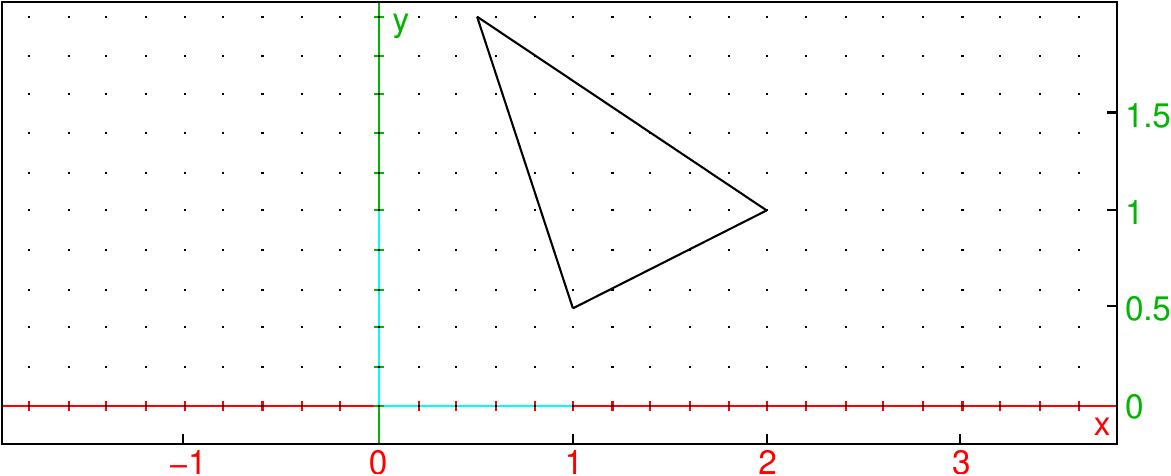
\includegraphics[width=0.75\textwidth]{xcas-tr.png}
\end{center}

\section{Basic commands}

\subsection{Clear the \texttt{DispG} screen: \texttt{erase}\index{erase}}

The \texttt{DispG} screen records all graphic commands
since the beginning of the session or the screen was last erased.  The
\texttt{Alt-D} command (or the menu command \texttt{Cfg
$\blacktriangleright$ Show $\blacktriangleright$ DispG}) brings up
this screen. 

The \texttt{erase} command clears the \texttt{DispG} screen without
restarting the session.  Entering\\
Input:
\begin{center}
  \tt
  erase
\end{center}
or:
\begin{center}
  \tt
  erase()
\end{center}
clears the \texttt{DispG} screen.  This can be useful for commands
such as \texttt{graph2tex}, which only takes into account the objects
on the \texttt{DispG} screen.

\subsection{Toggle the axes: \texttt{switch\_axes}\index{switch\_axes}}

The \texttt{switch\_axes} command shows, hides or toggles the 
coordinate axes on the graphics screen depending on whether the
argument is \texttt{1}, \texttt{0} or empty.
(This can also be controlled by a \texttt{show axes} checkbox in the
configuration panel brought up with the \texttt{cfg} button on the
graphic screen control panel.) 

Entering\\
Input:
\begin{center}
  \tt
  switch\_axes()
\end{center}
toggles whether or not the coordinate axes are shown in subsequent
graphic screens.  Rather than toggling,\\
Input:
\begin{center}
  \tt
  switch\_axes(1)
\end{center}
causes all later graphic screens to have the axes, and\\
Input:
\begin{center}
  \tt
  switch\_axes(0)
\end{center}
causes all later graphic screens to omit the axes.

When the axes are visible, they have tick marks whose
separation is determined by the X-tick and Y-tick values on the
graphic configuration screen.  Setting these values to 0 removes the
axes.

\subsection{Draw unit vectors in the plane:
\texttt{Ox\_2d\_unit\_vector}\index{Ox\_2d\_unit\_vector}
\texttt{Oy\_2d\_unit\_vector}\index{Oy\_2d\_unit\_vector}
\texttt{frame\_2d}\index{frame\_2d}}

The \texttt{Ox\_2d\_unit\_vector} command draws the unit vector in
the $x$-direction on a plane.\\
Input:
\begin{center}
  \tt
  Ox\_2d\_unit\_vector()
\end{center}
Output:
\begin{center}
   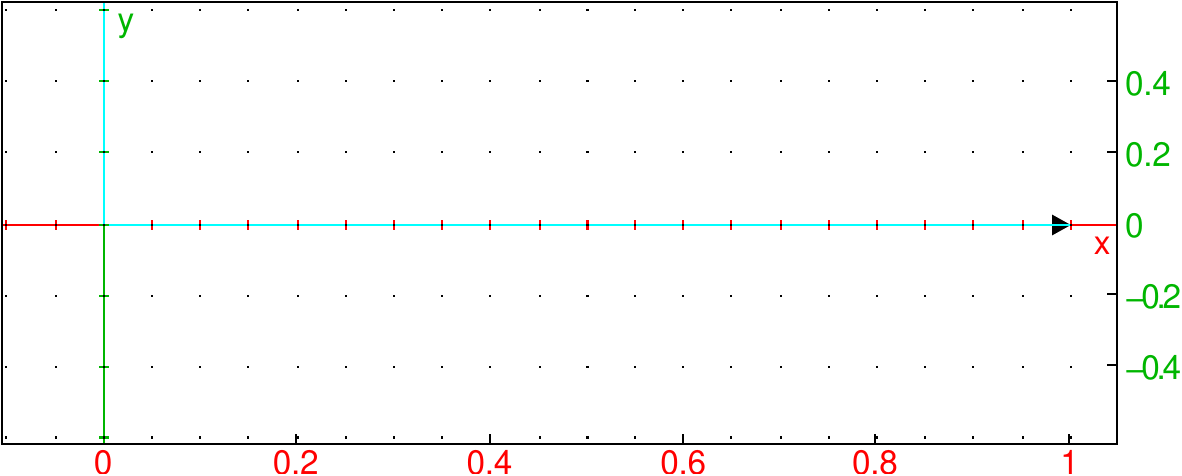
\includegraphics[width=0.75\textwidth]{xcas-unit-vector.png}
\end{center}
Similarly, the \texttt{Oy\_2d\_unit\_vector} command
draws the unit vector in the $y$ direction.
The \texttt{frame\_2d} command simultaneously draws both unit
vectors.

\subsection{Draw dotted paper: \texttt{dot\_paper}\index{dot\_paper}}

The \texttt{dot\_paper} command draws dotted paper.  This
command takes three mandatory arguments and two optional arguments.
The first argument is the spacing in the $x$ direction, the second
argument is the angle from the horizontal to draw the dots, and the
third argument is the spacing in the $y$ direction.  By default, the
dots extend in the $x$ and $y$ directions for the distances given in
the graphic configuration page accessible from the main menu; the
optional fourth and fifth 
arguments \texttt{x=xmin..xmax} and \texttt{y=ymin..ymax} change the
size of the dotted paper.\\
Input:
\begin{center}
  \tt
  dot\_paper(0.6,pi/2,0.6)
\end{center}
Output:
\begin{center}
 
\includegraphics[width=0.75\textwidth]{xcas-dot-paper.png}
\end{center}
Unchecking \texttt{Show Axes} on the \texttt{cfg} screen removes
the axes.

\subsection{Draw lined paper: \texttt{line\_paper}\index{line\_paper}}

The \texttt{line\_paper} command draws lined paper.  This
command takes two mandatory arguments and two optional arguments.
The mandatory arguments are
the spacing in the $x$ direction and the angle
from the horizontal to draw the lines.  The optional third and fourth
arguments, \texttt{x=xmin..xmax} and \texttt{y=ymin..ymax}, 
determine the size of the lined paper.\\
Input:
\begin{center}
  \tt
  line\_paper(0.6,pi/3)
\end{center}
Output:
\begin{center}
 
\includegraphics[width=0.75\textwidth]{xcas-line-paper.png}
\end{center}
Unchecking \texttt{Show Axes} on the \texttt{cfg} screen removes
the axes.

\subsection{Draw grid paper: \texttt{grid\_paper}\index{grid\_paper}}

The \texttt{grid\_paper} command draws grid paper.  This
command takes three mandatory arguments and two optional arguments.
The mandatory arguments are
the spacing in the $x$ direction, the the angle
from the horizontal to draw the grid, and the spacing
in the $y$ direction.  The optional fourth and fifth arguments, 
\texttt{x=xmin..xmax} and \texttt{y=ymin..ymax}, restrict the
size of the grid.\\
Input:
\begin{center}
  \tt
  grid\_paper(1,pi/2,1)
\end{center}
Output:
\begin{center}
 
\includegraphics[width=0.75\textwidth]{xcas-grid-paper.png}
\end{center}
Unchecking \texttt{Show Axes} on the \texttt{cfg} screen removes
the axes.

\subsection{Draw triangular paper: \texttt{triangle\_paper}}
\index{triangle\_paper}

The \texttt{triangle\_paper} command draws triangular paper.  This
command takes three mandatory and two optional arguments.  The
mandatory arguments are
the spacing in the $x$ direction, the angle
from the horizontal, and the spacing
in the $y$ direction.  The optional fourth and fifth arguments, 
\texttt{x=xmin..xmax} and \texttt{y=ymin..ymax}, restrict the
size of the grid.\\
Input:
\begin{center}
  \tt
  triangle\_paper(1,pi/2,1)
\end{center}
Output:
\begin{center}
   
\includegraphics[width=0.75\textwidth]{xcas-triangle-paper.png}
\end{center}
Unchecking \texttt{Show Axes} on the \texttt{cfg} screen removes the
axes.

\section{Display features of graphics}
\label{sec:dispfeat}

\subsection{Graphic features}

Graphic objects and graphic screens can have features, such as
labels and colors, that are only included when requested, and other
features, such as line width, which are configurable.  Some features
will be global, meaning that they will apply to the entire graphic
screen, and some will be local, meaning that they will only apply to
individual objects. 

\subsection{Parameters for changing features}

Graphical features are changed by giving appropriate values to
certain parameters.  Several values can be given at once with an
expression of the form \texttt{\textit{feature} = value1 + value2 + \dots}.
Some values can be set using optional arguments to graphic commands,
which will set the feature locally; namely, it will only apply to that
particular graphic object. Some values can be specified at the
beginning of a line, which will set the feature globally; it will
apply to all the graphic objects created on that line.  For some
features, both options are available.  

\subsubsection{Parameters for local features}
\index{thickness@\textit{thickness}}
\index{nstep@\textit{nstep}}
\index{tstep@\textit{tstep}}
\index{ustep@\textit{ustep}}
\index{vstep@\textit{vstep}}
\index{xstep@\textit{xstep}}
\index{ystep@\textit{ystep}}
\index{zstep@\textit{zstep}}
\index{frames@\textit{frames}}
\index{gl\_texture@\textit{gl\_texture}}
\label{sec:localfeatures}

Commands which create graphic objects, such as \texttt{triangle}, can
have optional arguments to change a features of the object.
For example, the argument \texttt{color = red} will make an object red.\\ 
Input:
\begin{center}
  \tt
  triangle(0,1,1+i,color=red)
\end{center}
Output:
\begin{center}
  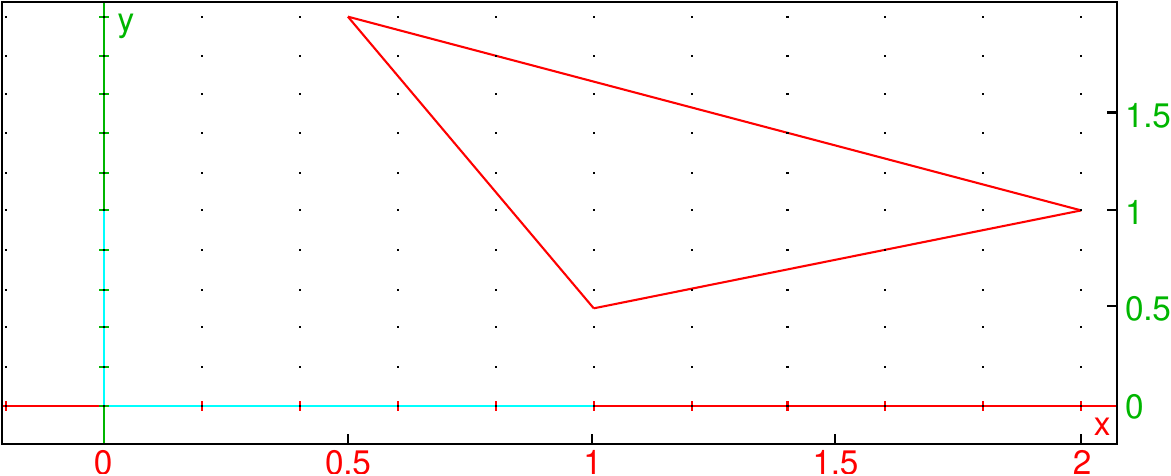
\includegraphics[width=0.75\textwidth]{xcas-red-triangle.png}
\end{center}

The features and their possible values are:
\begin{description}
  \item[\texttt{display} or \texttt{color}] These two parameter names
  have the same effect.  They control the following features.
  \begin{description}
  \item[Color]  The following values will change the color:
  \begin{itemize}
    \item An integer from \texttt{0} to \texttt{381}.\\
    Integers from 0 to 255 correspond to the color palette, integers from
    256 to 381 will be the spectrum of colors.\\
    The program
\begin{verbatim}
  rainbow() := {
    local j, C;
    C := [];
    for (j := 256; j < 382; j++) {
      C := append(C,square(j,j+1,color=j+filled));
      }
   }
\end{verbatim}
will show the colors;\\
Input:
\begin{center}
  \tt
  rainbow();
\end{center}
Output:
\begin{center}
  
\includegraphics[width=0.75\textwidth]{xcas-rainbow.png}
\end{center}
The number of a color is its $x$-coordinate.  To see just
one color, say the color corresponding to $n$ for $256 \le n \le 381$,
enter\\
Input:
\begin{center}
  \tt
  rainbow()[$n$-256]
\end{center}

    \item The names 
    \texttt{black}, \texttt{white}, \texttt{red}, \texttt{blue},
    \texttt{green}, \texttt{magenta}, \texttt{cyan} or \texttt{yellow}.
  \end{itemize}

  \item[Fill] The \texttt{filled} value creates a solid object.\\
  Input:
  \begin{center}
    \tt
    triangle(0,1,1+i,display=filled)
  \end{center}
  Output:
  \begin{center}
    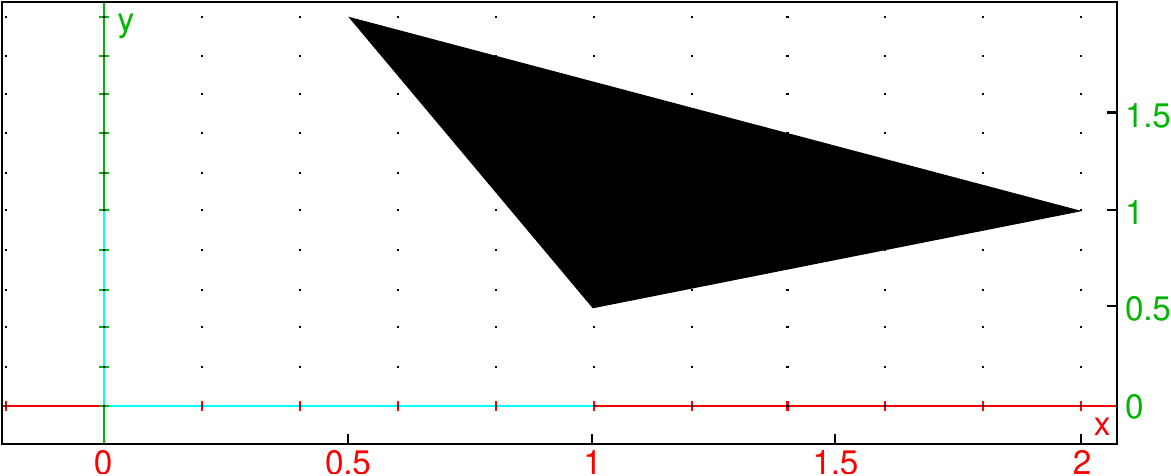
\includegraphics[width=0.75\textwidth]{xcas-filledtriangle.png}
  \end{center}
  \item[Point markers]  By default, points are drawn 
    with a small cross.  The following (self-explanatory) values
    change the marker.
    \begin{description}
      \item[\texttt{rhombus\_point}]
      \item[\texttt{square\_point}]
      \item[\texttt{cross\_point}]
      \item[\texttt{star\_point}]      
      \item[\texttt{plus\_point}]      
      \item[\texttt{point\_point}]      
      \item[\texttt{triangle\_point}]
      \item[\texttt{invisible\_point}]      
    \end{description}
    
    \item[Point width]   The values
    \texttt{point\_width\_1},\dots,\texttt{point\_width\_8}
    change the thickness of the lines in the point markers.

    \item[Line style]  The following (self-explanatory) values change
    the style of lines.
    \begin{description}
      \item[\texttt{solid\_line}]
      \item[\texttt{dash\_line}]
      \item[\texttt{dashdot\_line}]
      \item[\texttt{dashdotdot\_line}]      
      \item[\texttt{cap\_flat\_line}]      
      \item[\texttt{cap\_round\_line}]      
      \item[\texttt{cap\_square\_line}]
    \end{description}
    
    \item[Line widths]   The values
    \texttt{line\_width\_1},\dots,\texttt{line\_width\_8}
    change the thickness of the lines.
  \end{description}

  \item[\texttt{thickness}]  This controls line thickness, it can be
  an integer from 1 to 7.
  \item[\texttt{nstep}]  This sets the number of sampling points
  for three-dimensional objects.
  \item[\texttt{tstep}] This sets the step size of the
   parameter when drawing a one parameter parametric plot.
   \item[\texttt{ustep}] This sets the step size of the
   first parameter when drawing a two-parameter parametric plot.
   \item[\texttt{vstep}] This sets the step size of the
   second parameter when drawing a two-parameter parametric plot.
   \item[\texttt{xstep}] This sets the step size of the
   $x$ variable.
   \item[\texttt{ystep}] This sets the step size of the
   $y$ variable.
   \item[\texttt{zstep}] This sets the step size of the
   $z$ variable.
   \item[\texttt{frames}] This sets the number of
   graphs computed when an animated graph is created with the
   \texttt{animate} or \texttt{animate3d} command.
   \item[\texttt{legend}] This adds a legend to a graphic object and
   should be a string.  It is probably most useful when
   that object is a point or a polygon.  If the object is a polygon,
   the legend will be placed in the middle of the last side.  
   Other parameters for the graphic object will specify the color or
   position of the legend.
   % \item[\texttt{style}]  This only takes the value \texttt{point}.
   % If you set it to point, then lines will be drawn as dotted lines.
   \item[\texttt{gl\_texture}] This sets an
   image file to be put on the graphic object; it should be the name
   of the file.
\end{description}

\subsubsection{Parameters for global features}
\label{sec:globpar}

Parameters set at the beginning of a line change features on the
entire graphic screen.  It only takes effect
when the line ends with a graphic command.
For example, starting the line with \texttt{title=\textit{title
string}} will give the graphic screen a title.\\
Input:
\begin{center}
  \tt
  title = "Some triangles"; triangle(0,1,1+i); triangle(2,3,3+i);
\end{center}
Output:
\begin{center}
   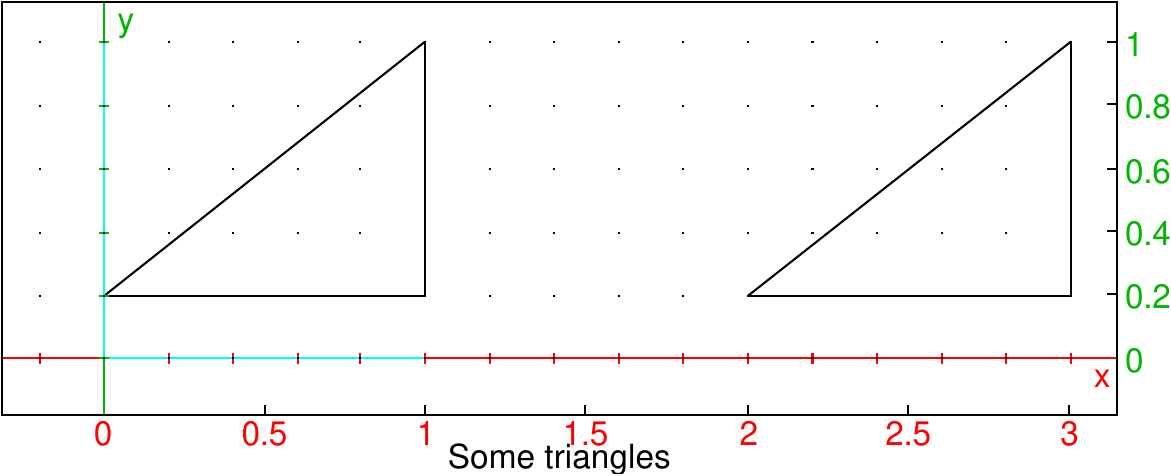
\includegraphics[width=0.75\textwidth]{xcas-some-triangles.png}
\end{center}

The parameters for global features and their possible values are:
\begin{description}
  \item[\texttt{axes}]
  This determines whether axes are shown or hidden; a value of
  \texttt{0} or \texttt{false} hides the axes, a value of
  \texttt{1} or \texttt{true} shows the axes.
  \item[\texttt{labels}]  This sets labels for the axes; it should be
  a list of two strings  \texttt{["\textit{x axis label}","\textit{y
  axis label}"]}.
  \item[\texttt{label}]
  This puts labels on the graphic screen in the following ways.
  \begin{itemize}
    \item 
    To set the units on the axes, it can be a list of two or three strings,
    \texttt{["\textit{x units}","\textit{y units}"]} or
    \texttt{["\textit{x units}","\textit{y units}","\texttt{z
    units}"]}.
    \item 
    To place a string at a particular point, it can
    be a list of two integers followed by a
    string.  The integers determine the point,
    starting from \texttt{[0,0]} in the top left of the
    screen.
  \end{itemize}
  \item[\texttt{title}]  This sets the title for the graphic window,
  it should be a string.
   \item[\texttt{gl\_texture}] This sets the wallpaper of the graphic
   window to be an image file, it should be the name of the file.
   \item[\texttt{gl\_x\_axis\_name},\texttt{gl\_x\_axis\_name},\texttt{gl\_x\_axis\_name}]
   These set the names of the axes.
   \item[\texttt{gl\_x\_axis\_unit},\texttt{gl\_x\_axis\_unit},\texttt{gl\_x\_axis\_unit}]
   These set the units of the axes.   
   \item[\texttt{gl\_x\_axis\_color},\texttt{gl\_x\_axis\_color},\texttt{gl\_x\_axis\_color}]
   These set the colors of the axes
   labels; they take the same color options as the local parameter
   \texttt{color}.
   \item[\texttt{gl\_ortho}]  This ensures that the graph is
   orthonormal when it is set to \texttt{1}.
   \item[\texttt{gl\_x},\texttt{gl\_y},\texttt{gl\_z}]
   These define the framing of the graph; they should be intervals
   \textit{min}\texttt{..}\textit{max}. (They are not compatible with
   interactive graphs.)
   \item[\texttt{gl\_xtick},\texttt{gl\_ytick},\texttt{gl\_ztick}]
   These determine the spacing of the ticks on the axes.
   \item[\texttt{gl\_shownames}]  This shows or hides object names, it
   can be \texttt{true} or \texttt{false}.
   \item[\texttt{gl\_rotation}]  This sets the axis of rotation for
   three-dimensional scene animations; it should be a direction vector
   \texttt{[$x$,$y$,$z$]}.
   \item[\texttt{gl\_quaternion}]  This sets the quaternion for viewing
   three-dimensional scenes; it should be a fourtuple
   \texttt{[$x$,$y$,$z$,$t$]}.   (This is not compatible with
   interactive graphs.)
\end{description}

\subsection{Commands for global display features}

\subsubsection{Add a legend: \texttt{legend}}
\index{legend}
\label{sec:addlegend}

The \texttt{legend} command takes two arguments and an optional third.  The
arguments are:
\begin{itemize}
  \item A position to put the legend.  This can either be a point or a
  list of two integers giving the number of pixels from the upper left
  hand corner.
  \item The legend itself, a string or a variable.
  \item An optional third parameter indicating where to put the legend
  relative to the point.  By default, it will be to the upper right of
  the point (\texttt{quadrant1}), but you can specify
  \texttt{quadrant1}, \texttt{quadrant2}, \texttt{quadrant3} or
  \texttt{quadrant4}.
\end{itemize}
For example, to put "hello" to the upper left of the point
$(1,1)$:\\
Input:
\begin{center}
  \tt
  legend(1+i,"hello",quadrant3)
\end{center}
or\\
Input:
\begin{center}
  \tt
  legend(1+i,quadrant3,"hello")
\end{center}
Output:
\begin{center}
  \tt
  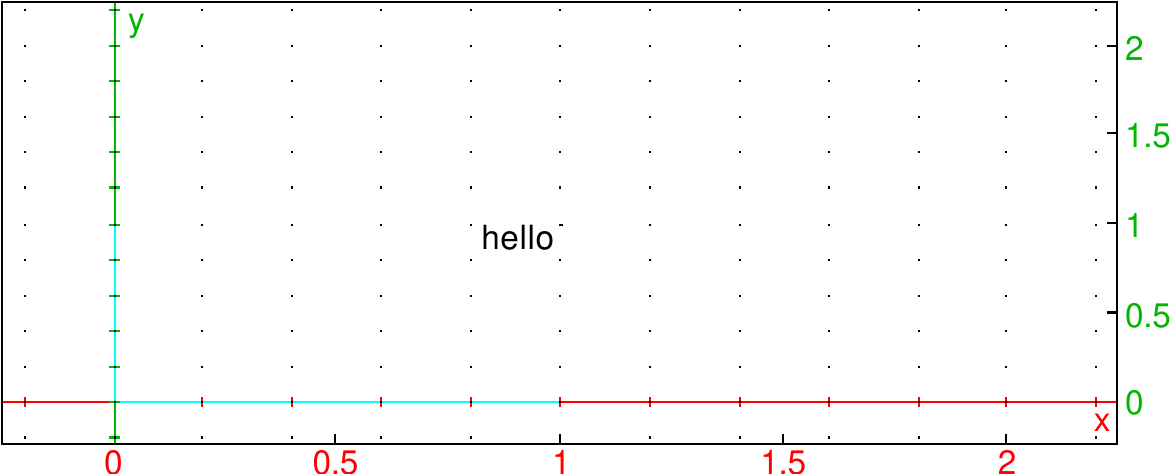
\includegraphics[width=0.75\textwidth]{xcas-hello-legend.png}
\end{center}

%To put a legend at an angle, see section \ref{sec:2dangle}.

\subsubsection{Change various features:\texttt{display, color}}
\index{display}\index{color}

The \texttt{display} command changes the properties of
graphics; the same properties that can also be changed with the \texttt{display} and
\texttt{color} parameters.  (See section \ref{sec:localfeatures}.)  
The \texttt{color} command is
the same as the \texttt{display} command.

The \texttt{display} command can draw objects with specified
properties.  In this case, the first argument will be a command to
create the object and the second argument will be a value for the 
\texttt{display} or \texttt{color} parameter.
Both\\
Input:
\begin{center}
  \tt
  display(triangle(0,1,1+i),red)
\end{center}
and\\
Input:
\begin{center}
  \tt
  triangle(0,1,1+i,display=red)
\end{center}
draw\\
Output:
\begin{center}
  \tt
  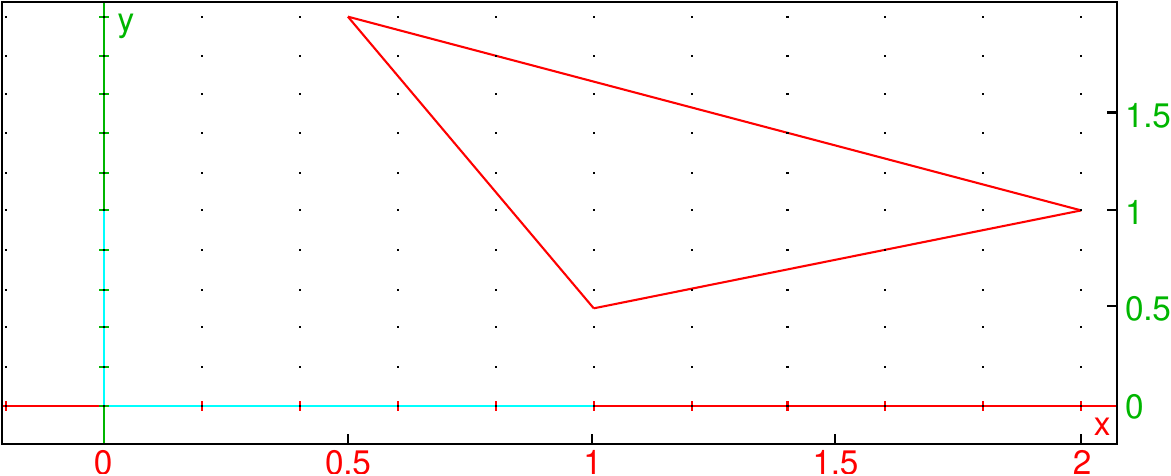
\includegraphics[width=.75\textwidth]{xcas-red-triangle.png}
\end{center}
Similarly, both\\
Input:
\begin{center}
  \tt
  triangle(0,1,1+i,display=filled)
\end{center}
and\\
Input:
\begin{center}
  \tt
  display(triangle(0,1,1+i),filled)
\end{center}
draw\\
Output:
\begin{center}
  \tt
  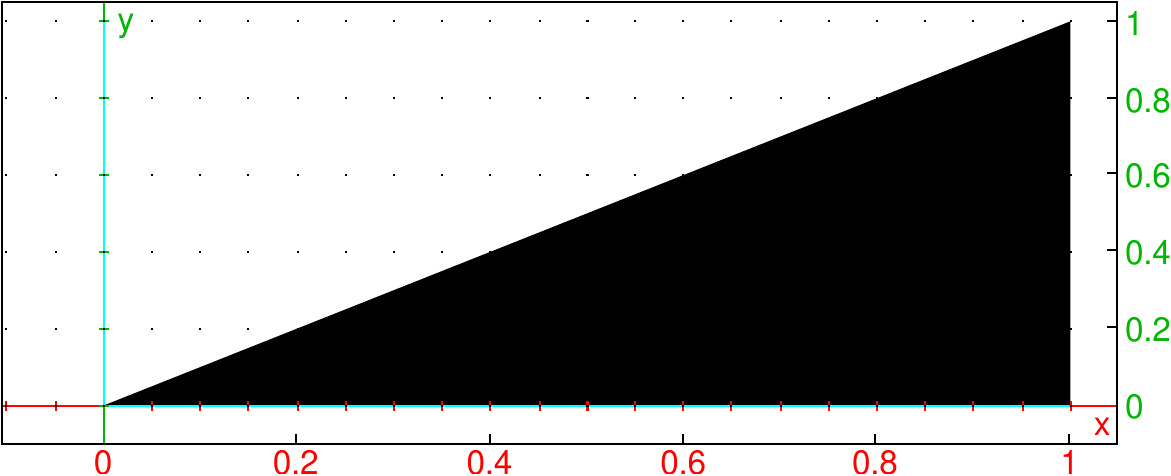
\includegraphics[width=0.75\textwidth]{xcas-trianglefilled.png}
\end{center}
The \texttt{display} command can also take a second argument of
\texttt{hidden\_name}.  By default, if a geometric object is named,
the drawing is labeled.\\ 
Input:
\begin{center}
  \tt
  A := triangle(0,1,1+i)
\end{center}
Output:
\begin{center}
  \tt
  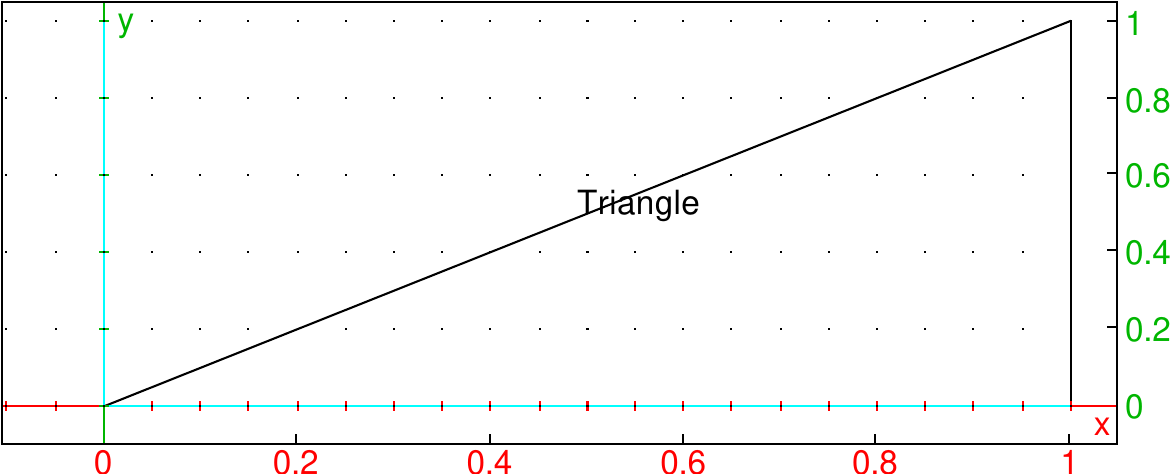
\includegraphics[width=0.75\textwidth]{xcas-triangleA.png}
\end{center}
Creating the object with the \texttt{display} command and the
\texttt{hidden\_name} argument will draw it without the label.\\
Input:
\begin{center}
  \tt
  display(A := triangle(0,1,1+i),hidden\_name)
\end{center}
Output:
\begin{center}
  \tt
  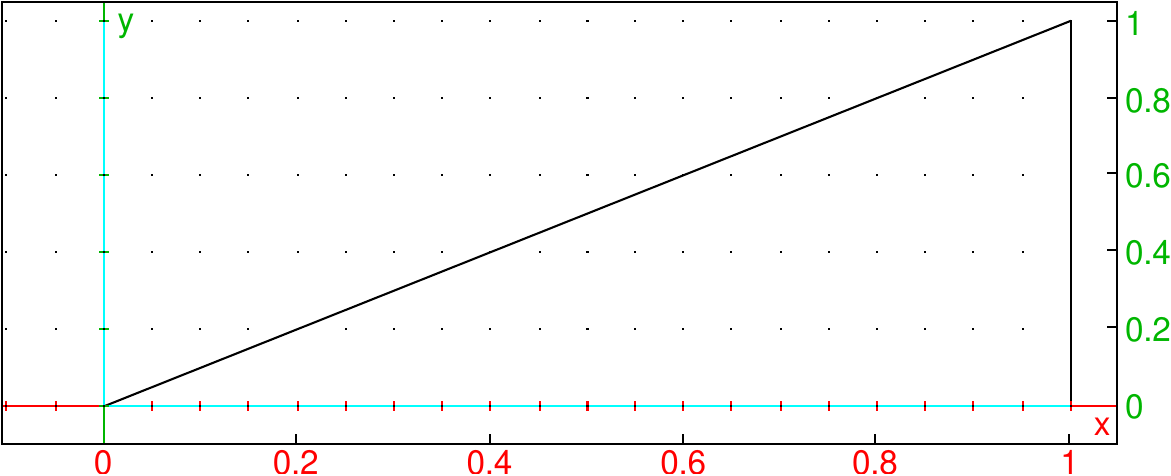
\includegraphics[width=0.75\textwidth]{xcas-triangleNoA.png}
\end{center}

The \texttt{display} command can also be used without drawing an
object, such as  \texttt{display(hidden\_name)} or
\texttt{display(filled)}.  In this case it will be a
global command; the display effect will apply to all objects
afterwards.  Entering \texttt{display(0)} will reset the display
parameters; afterwards, for example, the colors will be black, the
figures won't be filled, and the objects will have labels.

\section{Define geometric objects without drawing them: \texttt{nodisp}\index{nodisp}}

The \texttt{nodisp} command will define an object without displaying
it.  Setting a variable to a graphic object draws the object.\\
Input:
\begin{center}
  \tt
  C := point(1+i)
\end{center}
will define the point \texttt{C} as well as draw it.  Setting a
variable to a graphic object inside the \texttt{nodisp} command will
not draw the object.\\
Input:
\begin{center}
  \tt
  nodisp(C:= point(1+i))
\end{center}
will define the point $C$  but not display it.  This is
equivalent to following the command with \texttt{:;},
\\
Input:
\begin{center}
  \tt
  C := point(1+i):;
\end{center}

To define a point as above and display it without the
label, enter the point's name;\\
Input:
\begin{center}
  \tt
  C
\end{center}
Alternatively, define the point within an
\texttt{eval} statement;\\
Input:
\begin{center}
  \tt
  eval(C := point(1+i))
\end{center}
defines $C$ as the point, displays the point, but doesn't display the
label.  To later display the point with a label, use the
\texttt{legend} command.\\
Input:
\begin{center}
  \tt
  legend(C,"C")
\end{center}
or:
\begin{center}
  \tt
  point(affix(C),legend="C")
\end{center}
Output:
\begin{center}
  \tt
  \includegraphics[width=0.75\textwidth]{xcas-legendC.png}
\end{center}
In this case, the string "C" can be replaced with any other string 
as a label.  Alternatively, redefine the
variable as itself;\\
Input:
\begin{center}
  \tt
  C := C
\end{center}
prints $C$ with its label.

\section{Geometric demonstrations: \texttt{assume}\index{assume}}

Variables should be unspecified to demonstrate a general geometric
result, but need to have specific values when drawing.  There are a
couple of different approaches to deal with this.

One approach is to use the \texttt{assume} command.  If a variable is 
\emph{assumed} to have a value, then that value will be used in
graphics but the variable will still be unspecified for calculations.
For example,\\
Input:
\begin{center}
  \tt
  assume(a = 2.1)
\end{center}
then 
\\
Input:
\begin{center}
  \tt
  A := point(a + i)
\end{center}
will draw a point at the coordinate $(2.1,1)$,\\
Output:
\begin{center}
  \tt
  \includegraphics[width=0.75\textwidth]{xcas-assumea.png}
\end{center}
but the variable $a$ will still be treated as a variable in
calculations;\\
Input:
\begin{center}
  \tt
  distance(0,A)
\end{center}
Output:
\begin{center}
  \tt
  sqrt((-a)\^{}2 + 1)
\end{center}

Another approach would be to use \texttt{point} or \texttt{pointer}
mode in a geometry screen.  If there isn't a geometry screen showing,
the command \texttt{Alt-G} or the \texttt{Geo$\blacktriangleright$New
figure 2d} menu will open a screen.  Clicking on the 
\texttt{Mode} button right above the graphic screen and choosing 
\texttt{pointer} or \texttt{point} will put the screen in
\texttt{pointer} or \texttt{point} mode.
If a point is defined and displayed, such as 
with \texttt{A := point(2.1 + i)}, then clicking on the name of the
point (\texttt{A} in this case) with the right mouse button will bring
up a configuration screen.  As long as there is a point defined with
non-symbolic values, there will be a \texttt{symb} box on the configuration
screen.  Selecting the \texttt{symb} box and
choosing \texttt{OK} will  be equivalent to the commands
\texttt{assume(Ax=[2.1,-8.16901408451,8.16901408451])}
and \texttt{assume(Ay = [1, -5.0, 5.0]}, this will bring up
two lines beneath the arrows to the right of the screen which can be
used to change the assumed values of \texttt{Ax} and \texttt{Ay}.
Also, the point \texttt{A} will be redefined as \texttt{point(Ax,Ay)}.
\begin{center}
  \tt
  \includegraphics[width=0.75\textwidth]{xcas-assumespoint.png}
\end{center}

\section{Points in the plane}

\subsection{Points and complex numbers}

The \emph{affix} of a point $(a,b)$ in the plane is the complex number
$a + bi$.   In this section, when a command take points as arguments,
the points can be specified by a pair or by a complex number.

\subsection{The point in the plane: \texttt{point}}
\index{point}
\label{sec:2dpoint}

See section \ref{sec:3dpoint} for points in space.

In the 2-d geometry screen in point mode, clicking on a point with the
left mouse button will choose that point.  Points chosen this way are
automatically named, first with \texttt{A}, then \texttt{B}, etc.  

Alternatively, the \texttt{point} command chooses a point, where the
point $(a,b)$ is specified by either the two coordinates \text{a,b}, a
list \texttt{[a,b]} of the coordinates, or the affix \texttt{a + b*i}.\\
Input:
\begin{center}
  \tt
  A := point(2,1)
\end{center}
or:
\begin{center}
  \tt
  A := point([2,1])
\end{center}
or\\
Input:
\begin{center}
  \tt
  A := point(2 + i)
\end{center}
Output:
\begin{center}
  \tt
  \includegraphics[width=0.75\textwidth]{xcas-2dpoint.png}
\end{center}
(The marker used to indicate the point can be changed; see section
\ref{sec:localfeatures}.)

If the \texttt{point} command has two numbers for arguments, at least
one of which is complex but not real, then it will choose two points.
Entering\\
Input:
\begin{center}
  \tt
  A := point(1,2*i)
\end{center}
or:
\begin{center}
  \tt
  A := point([1,2*i])
\end{center}
will choose two points named \texttt{A}; one with affix $1$ and
one with affix \texttt{2i}.

\subsection{The difference and sum of two points in the
plane:\texttt{+, -}}
\index{+}\index{-}

Let \texttt{A} and \texttt{B} be two points in the plane, with affixes
$a_1 + i a_2$ and $b_1 + ib_2$ respectively.\\
Input:
\begin{center}
  \tt
  A:= point(1 + 2*i); B := point(3+4*i)
\end{center}
\begin{itemize}
  \item The difference \texttt{B-A} returns the affix 
  $(b_1-a_1)+i(b_2-a_2)$, which represents the vector $AB$.\\
Input:
\begin{center}
  \tt
  vector(A,B); vector(point(0),point(B-A))
\end{center}
Output:
\begin{center}
  \includegraphics[width=0.75\textwidth]{xcas-subpts.png}
\end{center}
\item The sum \texttt{B+A} returns the affix 
  $(b_1+a_1)+i(b_2+a_2)$.  If \texttt{D := point(B+A)}, then
  \texttt{BD = OA}.\\
Input:
\begin{center}
  \tt
   D := point(B + A);\\
   segment(B,D); segment(point(0),A)
\end{center}
Output:
\begin{center}
  \includegraphics[width=0.75\textwidth]{xcas-addpts.png}
\end{center}
\end{itemize}

Note that \texttt{-A} is the point symmetric to \texttt{A} with
respect to the origin.  

The sum of three points \texttt{A + B + C} can
be viewed as the translate of \texttt{C} by the vector \texttt{A + B}.
So if \texttt{A} or \texttt{B} contains parameters, you should write
this as \texttt{C + (A + B)} or \texttt{evalc(A + B) + C}.

\subsection{Define random points in the plane: \texttt{point2d}\index{point2d}}

The \texttt{point2d} command defines a random point whose
coordinates are integers between -5 and 5.  This command takes a name
as an argument and assigns the point to the name.  For example,\\
Input:
\begin{center}
  \tt
  point2d(A)
\end{center}
assigns \texttt{A} to a random point.  Once assigned, the point
is fixed.  The command can also take a sequence of names, and
will assign separate random points to each name.  For example, to
generate a random triangle, first generate three random points\\
Input:
\begin{center}
  \tt
  point2d(A,B,C)
\end{center}
and then use them for a triangle\\
Input:
\begin{center}
  \tt
  triangle(A,B,C)
\end{center}

\subsection{Points in polar coordinates:
\texttt{polar\_point}\index{polar\_point}, \texttt{point\_polar}\index{point\_polar}}

To specify a point in polar coordinates, enter the polar
representation of complex numbers.  For example, the command\\
Input:
\begin{center}
  \tt
  point(2*exp(i * pi/4))
\end{center}
draws the point with polar coordinates $r=2$, $\theta = \pi/4$.
The \texttt{polar\_point} command does this in an easier way, it
takes $r$ and $\theta$ as arguments.  
The command\\
Input:
\begin{center}
  \tt
  polar\_point(2,pi/4)
\end{center}
creates the same point as before.

\subsection{Find a point of intersection of two objects in the plane: \texttt{single\_inter}\index{single\_inter} \texttt{line\_inter}\index{line\_inter}}
\label{sec:single2dintersection}

See section \ref{sec:3dsingleintersection} for single points of intersection of objects
in space.

The \texttt{single\_inter} (or the \texttt{line\_inter}) command takes
two geometric objects as arguments
and returns one of the points of intersection of the two objects.  

The \texttt{single\_inter} command optionally takes a third
argument, which can be a point or a list of points.  If the optional
argument is 
a single point, then \texttt{single\_inter} returns the point of
intersection \emph{closest} to the optional argument.  If the optional
argument is a list of points, then \texttt{single\_inter} tries to
return a point of intersection not in the list.

For example, the unit circle \texttt{circle(0,1)} and line
\texttt{line(-1,i)} intersect at the points
$(-1,0)$ and $(0,1)$.  Entering\\
Input:
\begin{center}
  \tt
  single\_inter(circle(0,1),line(-1,i))
\end{center}
draws the point $(-1,0)$.  To draw the other
point, enter\\
Input:
\begin{center}
  \tt
  single\_inter(circle(0,1),line(-1,i),[-1])
\end{center}
and \texttt{Xcas} will draw $(0,1)$.  Similarly, since this second
point of intersection is closest to $(0,1/2)$, entering\\
Input:
\begin{center}
  \tt
  single\_inter(circle(0,1),line(-1,i),i/2)
\end{center}
also draws the second point.

\subsection{Find the points of intersection of two geometric objects
in the plane: \texttt{inter}\index{inter}}
\label{sec:2dintersection}

See section \ref{sec:3dintersection} for points of intersection of objects
in space.

The \texttt{inter} command takes
two geometric objects as arguments
and returns a list of the points of intersection of the two objects.  

The \texttt{inter} command optionally takes a point as a third argument.
In this case, \texttt{inter} returns the point of intersection
\emph{closest} to this argument.

For example, entering\\
Input:
\begin{center}
  \tt
  inter(circle(0,1),line(1,i))
\end{center}
draws the points at $(1,0)$ and $(0,1)$.
To get just one of the points, use the usual list indices.\\
Input:
\begin{center}
  \tt
  inter(circle(0,1),line(1,i))[0]
\end{center}
draws just one of the points.
To get the point closest to $(0,1/2)$, enter\\
Input:
\begin{center}
  \tt
  inter(circle(0,1),line(1,i),i/2)
\end{center}

\subsection{Find the orthocenter of a triangle in the plane: \texttt{orthocenter}\index{orthocenter}}

The \texttt{orthocenter} command take a triangle (or three
points representing the vertices of a triangle) as argument and returns the
orthocenter of the triangle.  Entering\\
Input:
\begin{center}
  \tt
  orthocenter(triangle(0,1+i,-1+i))
\end{center}
or\\
Input:
\begin{center}
  \tt
  orthocenter(0,1+i,-1+i)  
\end{center}
draws the point $(0,0)$, the orthocenter of the
triangle.

\subsection{Find the midpoint of a segment in the plane: \texttt{midpoint}\index{midpoint}}
\label{sec:2dmidpt}

See section \ref{sec:3dmidpt} for midpoints in space.

The \texttt{midpoint} command takes two points (or a list of two
points) as arguments and draws the midpoint of the segment
determined by these points.  

\subsection{The barycenter in the plane: \texttt{barycenter}\index{barycenter}}
\label{sec:2dbarycenter}

See section \ref{sec:3dbarycenter} for barycenters of objects in
space.

The \texttt{barycenter} command draws the barycenter of a set of
weighted points.  The points and their weights (real numbers) can be
given in three different ways.
\begin{enumerate}
  \item A sequence of lists of length two.\\
  The first element of each list is a point and the second element is
  the weight of the point.
  \item A matrix with two columns.\\
  The first column of the matrix contains the points and the
  second column contains the corresponding weights.
  \item A matrix with two rows and more than two columns.\\
  The first row contains the points and the second row the
  corresponding weights.
\end{enumerate}

For example, the following commands will draw the barycenter of the
points $(1,1)$ with weight $1$, $(1,-1)$ with weight $1$ and $(1,4)$
with weight $2$.\\
Input:
\begin{center}
  \tt
  barycenter([1 + i,1],[1 - i,1],[1 + 4*i, 2])
\end{center}
or:
\begin{center}
  \tt
  barycenter([[1 + i,1],[1 - i,1],[1 + 4*i, 2]])
\end{center}
or:
\begin{center}
  \tt
  barycenter([[1 + i, 1 - i, 1 + 4*i],[1,1,2]])
\end{center}
Output:
\begin{center}
  \tt
  \includegraphics[width=0.75\textwidth]{xcas-barycenter.png}
\end{center}

\subsection{The isobarycenter of $n$ points in the plane: \texttt{isobarycenter}\index{isobarycenter}}
\label{sec:2disobarycenter}

See section \ref{sec:3disobarycenter} for isobarycenters of objects in
space.

The \texttt{isobarycenter} command takes a list (or sequence) of
points and draws the isobarycenter, which is the barycenter when all
the points are equally weighted.

\subsection{The center of a circle in the plane: \texttt{center}\index{center}}

The \texttt{center} command takes as argument a circle and returns and draws the
center.\\
Input:
\begin{center}
  \tt
  C := center(circle(point(1+i),1))
\end{center}
Output:
\begin{center}
  \includegraphics[width=0.75\textwidth]{xcas-center.png}
\end{center}

\subsection{The vertices of a polygon in the plane:
\texttt{vertices}\index{vertices}, \texttt{vertices\_abc}\index{vertices\_abc}}

The \texttt{vertices} command (or \texttt{vertices\_abc}) takes as argument a
polygon.

\texttt{vertices} returns a list of the vertices of the polygon and
draws them.\\
Input:
\begin{center}
  \tt
  vertices(equilateral\_triangle(0,2))
\end{center}
Output:
\begin{center}
  \includegraphics[width=0.75\textwidth]{xcas-vertices.png}
\end{center}
Input:
\begin{center}
  \tt
  C := vertices(equilateral\_triangle(0,2))[2]
\end{center}
Output:
\begin{center}
  \includegraphics[width=0.75\textwidth]{xcas-vertices2.png}
\end{center}

\subsection{The vertices of a polygon in the plane, closed: \texttt{vertices\_abca}\index{vertices\_abca}}

The \texttt{vertices\_abca} command takes as argument a polygon.

\texttt{vertices\_abca} returns the ``closed'' list of vertices (it
repeats the beginning vertex) and draws them.
% Input:
% \begin{center}
%   \tt
%   vertices\_abca(equilateral\_triangle(0,2))
% \end{center}
% Output:
% \begin{center}
%   \includegraphics[width=0.75\textwidth]{xcas-vertices_abca.png}
% \end{center}

\subsection{A point on a geometric object in the plane: \texttt{element}\index{element}}
\label{sec:element}

The \texttt{element} command is most useful in a two-dimensional
geometry screen; it creates objects that are
restricted to a geometric figure.

\texttt{element} takes different types of arguments:
\begin{itemize}
  \item An interval $a..b$ and an optional initial value (by default
  $(a+b)/2$) and step size (by default $(b-a)/100$).
  
  This creates a parameter restricted to the interval, with the
  given initial value and whose value can be changed in the given step
  sizes. 

  For example, the command \texttt{t := element(0..pi)}  creates a
  parameter \texttt{t} which can take on values between $0$ and $\pi$
  and has initial value $\pi/2$.  It also creates a slider labeled
  \texttt{t} which can be used to change the values.  The values of
  any later formulas involving \texttt{t} will change with \texttt{t}.
  
  \item A curve and an optional initial value (by default $1/2$).  
  
  This creates a point which will be restricted to the curve,
  the initial position of the point is determined by setting the
  parameter (in the default parameterization of the object) to the
  initial value.  If the point can be moved by the mouse (as it can
  when the geometry screen is in \texttt{Pointer} mode), then the
  motion will be restricted to the geometric object.
  
  For example, the command \texttt{A := element(circle(0,2))} 
  creates a point labeled \texttt{A} whose position is restricted to
  the circle of radius $2$ centered at the origin.  Since the circle
  has default parameterization $2\exp(i t)$, \texttt{A} starts out at
  $2\exp(i/2)$.

  \item A polygon or polygonal line \texttt{PL} with $n$ sides and 
  \texttt{[floor($t$),frac($t$)]}, where $t$ is a variable previously
  defined by \texttt{$t$ = element(0..$n$)}.
  
  This creates a point restricted to the polygonal line.  With the
  sides numbered starting at $0$, the value of \texttt{floor($t$)}
  determines which side the point is on, and the value of
  \texttt{frac($t$)} determines how far along the side the point is.
\end{itemize}

If a point $A$ (corresponding to the complex number $a$) is defined as
an element of a curve $C$ and $B$ is a point (corresponding to the
complex number $b$), then $A + B$ will be a point on $C$; it will be
the projection onto $C$ of the point corresponding to $a + b$.

Note that in this case, if $B'$ is another point, then $A + (B - B')$
isn't the same as $A + B - B'$.  The expression $A + (B - B')$ is
interpreted as adding the point $A$, defined as a point on $C$, to the
point $B - B'$, and so the sum will be on $C$.  The expression $A + B
- B'$ is interpreted as $(A + B) - B'$, and so the point $B'$ is not
being added to a point defined as an element of the curve $C$, and so
this sum may not be on $C$.

\section{Lines in plane geometry}

\subsection{Lines and directed lines in the plane: \texttt{line}\index{line}}
\label{sec:2dlines}

See section \ref{sec:3dlines} for lines in space.

The \texttt{line} command returns and draws a directed line given one of the
following types of arguments:
\begin{itemize}
  \item Two points or a list of two points.\\
  The direction of the line is from the first point
  to the second point.
  \item A point and a slope given by \texttt{slope=\textit{value}}.\\
  The direction of the line is determined by the slope.
  \item A point and  direction vector (in the form
  \texttt{[$u_1$,$u_2$]}).\\
  The direction of the line is given by the direction vector.
  \item An equation of the form \texttt{a*x+b*y+c=0}.\\
  The direction of the line is given by \texttt{[b,-a]}.
\end{itemize}
Input:
\begin{center}
  \tt
  line(0,1+i)
\end{center}
or:
\begin{center}
  \tt
  line(1+i,slope=1)
\end{center}
or:
\begin{center}
  \tt
  line(1+i,[3,3])
\end{center}
or:
\begin{center}
  \tt
  line(y - x = 0)
\end{center}
Output:
\begin{center}
  \includegraphics[width=0.75\textwidth]{xcas-line.png}
\end{center}

\textbf{Warning:} To draw a line with an additional argument for color
(such as \texttt{color = blue}), this argument must be the third
argument.  In particular, for a list of two points to
specify a line in this command, the list must be turned into a sequence, such as
with \texttt{op}.  For example, given a list \texttt{L} of two
points (possibly the result of a different command) which determines a
line, to draw the line \texttt{blue} enter
\texttt{line(op(L),color=blue)}; entering
\texttt{line(L,color=blue)} results in an error.

\subsection{Half-lines in the plane: \texttt{half\_line}}
\index{half\_line}
\label{sec:2dhalflines}

See section \ref{sec:3dhalflines} for half-lines in space.

The \texttt{half\_line} command takes as argument two points or a list of two
points.

\texttt{half\_line} returns and draws the ray from the first point
through the second.\\
Input:
\begin{center}
  \tt
  half\_line(0,-1+i)
\end{center}
Output:
\begin{center}
  \includegraphics[width=0.75\textwidth]{xcas-halfline.png}
\end{center}

\subsection{Line segments in the plane: \texttt{segment}\index{segment} \texttt{Line}\index{Line}}
\label{sec:2dsegments}

See section \ref{sec:3dsegments} for segments in space.

The \texttt{segment} command and the \texttt{Line} command draw line
segments.  (The \texttt{segment} command can also draw vectors, see
section \ref{sec:2dvectors}.)

\texttt{segment} takes as argument two points or a list of two points.

\texttt{segment} returns the corresponding line segment and draws it.

\texttt{Line} takes as argument four real numbers, the first two
represent the coordinates of the beginning of the segment and the last
two represent the end.

\texttt{Line} returns the line segment and draws it.

\noindent
\textbf{Example.}\\
Input:
\begin{center}
  \tt
  segment(-1,1+i)    
\end{center}
or:
\begin{center}
  \tt
  segment(point(-1),point(1,1))
\end{center}
or:
\begin{center}
  \tt
  Line(-1,0,1,1)
\end{center}
Output:
\begin{center}
  \includegraphics[width=0.75\textwidth]{xcas-segment.png}
\end{center}

\subsection{Vectors in the plane: \texttt{segment}\index{segment} \texttt{vector}\index{vector}}
\label{sec:2dvectors}

See section \ref{sec:3dvectors} for vectors in space.

The \texttt{segment} and \texttt{vector} commands return and draw vectors.
(The \texttt{segment} command can also draw line segments, see section
\ref{sec:2dsegments}.)

\texttt{segment} takes as arguments a point and a vector.
The point indicates the beginning of the result and the vector (given
as a list of coordinates) the direction.

\texttt{segment} returns and draws the corresponding vector as a line
segment.  If the arguments are \texttt{P} and \texttt{V}, then command
draws the segment from \texttt{P} to \texttt{P+V}.\\
Input:
\begin{center}
  \tt
  segment([-1,0],[1,1])
\end{center}
Output:
\begin{center}
  \includegraphics[width=0.75\textwidth]{xcas-segvec.png}
\end{center}

\texttt{vector} takes as arguments two points (or a list with two
points) or a point and a vector.

\texttt{vector} returns and draws the corresponding vector.  If the
arguments are two points, the vector goes from the first
to the second point; if the arguments are a point and a vector, then
the vector starts at the given point.\\
Input:
\begin{center}
  \tt
  vector([-1,0],[1,i])
\end{center}
or:
\begin{center}
  \tt
  vector(-1,i)
\end{center}
or:
\begin{center}
  \tt
  V := vector(1,2+i):; vector(-1,V)
\end{center}
Output:
\begin{center}
  \includegraphics[width=0.75\textwidth]{xcas-vect.png}
\end{center}

\subsection{Parallel lines in the plane: \texttt{parallel}\index{parallel}}
\label{sec:2dparallel}

See section \ref{sec:3dparallel} for parallel lines in space.

The \texttt{parallel} command takes as argument a point and a line.

\texttt{parallel} returns and draws the line parallel to the given
line passing through the given point.\\
Input:
\begin{center}
  \tt
  parallel(0,line(1,i))
\end{center}
Output:
\begin{center}
  \includegraphics[width=0.75\textwidth]{xcas-parallel.png}
\end{center}

\subsection{Perpendicular lines in the plane: \texttt{perpendicular}\index{perpendicular}}
\label{sec:2dperp}

See section \ref{sec:3dperp} for perpendicular lines in space.

The \texttt{perpendicular} command takes as arguments either a point and a line,
or three points (the last two points determining a line).

\texttt{perpendicular} returns and draws the line perpendicular to the
given line passing through the given point.\\
Input:
\begin{center}
  \tt
  perpendicular(0,line(1,i))
\end{center}
or:
\begin{center}
  \tt
  perpendicular(0,1,i)
\end{center}
Output:
\begin{center}
  \includegraphics[width=0.75\textwidth]{xcas-perp.png}
\end{center}

\subsection{Tangents to curves in the plane: \texttt{tangent}\index{tangent}}
\label{sec:2dtangents}

See section \ref{sec:3dtangents} for tangents in space.

The \texttt{tangent} command takes as arguments either a curve and a point, or a
point defined with \texttt{element} (see section \ref{sec:element}) using a curve and
parameter value.

\texttt{tangent} returns and draws the list of lines tangent to the
curve passing through the given point.\\
Input:
\begin{center}
  \tt
  tangent(circle(0,1),1+i)
\end{center}
Output:
\begin{center}
  \includegraphics[width=0.75\textwidth]{xcas-tangent1.png}
\end{center}
Input:
\begin{center}
  \tt
  t := element(0..pi,pi/4):; A := element(circle(0,1),t):; tangent(A)
\end{center}
Output:
\begin{center}
  \includegraphics[width=0.75\textwidth]{xcas-tangent2.png}
\end{center}

When \texttt{tangent} is called with an element,
the tangent will change along with the point on the element.

\subsection{The median of a triangle in the plane: \texttt{median\_line}\index{median\_line}}

The \texttt{median\_line} command takes as argument three points representing the
vertices of a triangle.

\texttt{median\_line} returns and draws the median line, through the
point given by the first argument and bisecting the segment determined
by the other two arguments.\\
Input:
\begin{center}
  \tt
  median\_line(0,1,i)
\end{center}
Output:
\begin{center}
  \includegraphics[width=0.75\textwidth]{xcas-median.png}
\end{center}

\subsection{The altitude of a triangle: \texttt{altitude}\index{altitude}}

The \texttt{altitude} command takes as argument three points representing the
vertices of a triangle.

\texttt{altitude} returns and draws the altitude line, through the
point given by the first argument and perpendicular to the line determined
by the other two arguments.\\
Input:
\begin{center}
  \tt
  altitude(0,1,i)
\end{center}
Output:
\begin{center}
  \includegraphics[width=0.75\textwidth]{xcas-altitude.png}
\end{center}

\subsection{The perpendicular bisector of a segment in the plane: \texttt{perpen\_bisector}\index{perpen\_bisector}}
\label{sec:2dperpbis}

See section \ref{sec:3dperpbis} for perpendicular bisectors in space.

The \texttt{perpen\_bisector} command takes as argument a line segment or two
points representing the end points of a line segment.

\texttt{perpen\_bisector} returns and draws the perpendicular bisector
of the segment.\\
Input:
\begin{center}
  \tt
  perpen\_bisector(1,i)
\end{center}
or:
\begin{center}
  \tt
  perpen\_bisector(segment(1,i))
\end{center}
Output:
\begin{center}
  \includegraphics[width=0.75\textwidth]{xcas-perpbisect.png}
\end{center}

The \texttt{perpen\_bisector} command can also take two lines as segments, in
which case it returns and draws the perpendicular bisector of the
segment from the first point defining the first line and the second
point defining the second line.

\subsection{The angle bisector: \texttt{bisector}\index{bisector}}

The \texttt{bisector} command takes as argument three points or a list of three
points.  The first point represents the vertex of an angle; the
remaining two points will be on the two sides of the angle.

\texttt{bisector} returns and draws the angle bisector.\\
Input:
\begin{center}
  \tt
  bisector(0,1,i)
\end{center}
Output:
\begin{center}
  \includegraphics[width=0.75\textwidth]{xcas-bisector.png}
\end{center}

\subsection{The exterior angle bisector: \texttt{exbisector}}
\index{exbisector}

The \texttt{exbisector} command takes as argument three points or a list of three
points.  

\texttt{exbisector} returns the bisector of the exterior angle of the
triangle determined by the points; the first point is the vertex of
the angle, the opposite of the first and second points determine one
side of the angle and the first and third determine the second side.\\
Input:
\begin{center}
  \tt
  exbisector(0,1,i)
\end{center}
Output:
\begin{center}
  \includegraphics[width=0.75\textwidth]{xcas-exbisector.png}
\end{center}

\section{Triangles in the plane}

See section \ref{sec:3dtriangles} for triangles in space.

\subsection{Arbitrary triangles in the plane: \texttt{triangle}\index{triangle}}
\label{sec:2dtricommand}

See section \ref{sec:3dtricommand} for the \texttt{triangle} command
in space.

The \texttt{triangle} command takes as arguments three points or a list of three
points.  

\texttt{triangle} returns and draws the triangle with the given
vertices.\\
Input:
\begin{center}
  \tt
  triangle(-1,i,1+i)
\end{center}
Output:
\begin{center}
  \includegraphics[width=0.75\textwidth]{xcas-triangle.png}
\end{center}

\subsection{Isosceles triangles in the plane: \texttt{isosceles\_triangle}\index{isosceles\_triangle}}
\label{sec:2disotriangles}

See section \ref{sec:3disotriangles} for isosceles triangles in space.

The \texttt{isosceles\_triangle} command takes three arguments and an optional
fourth.  The three mandatory arguments are two points \texttt{A}
and \texttt{B} and an angle $\theta$.

\texttt{isosceles\_triangle} returns and draws the isosceles triangle 
\texttt{ABC}, where \texttt{AB} and \texttt{AC} are equal sides and 
$\theta$ is the angle from \texttt{AB} to \texttt{AC}.\\
Input:
\begin{center}
  \tt
  isosceles\_triangle(i, 1, -3*pi/4)
\end{center}
Output:
\begin{center}
  \includegraphics[width=0.75\textwidth]{xcas-isotriangle.png}
\end{center}
The optional argument needs to be a variable name,
which is assigned to vertex \texttt{C}.\\
Input:
\begin{center}
  \tt
  isosceles\_triangle(i, 1, -3*pi/4,C)  
\end{center}
Output:
\begin{center}
  \tt
  \includegraphics[width=0.75\textwidth]{xcas-isotriangleC.png}
\end{center}
Input:
\begin{center}
  \tt
  normal(affix(C))
\end{center}
Output:
\begin{center}
  \tt
  -sqrt(2) + i
\end{center}

\subsection{Right triangles in the plane: \texttt{right\_triangle}\index{right\_triangle}}
\label{sec:2dright}

See section \ref{sec:3dright} for right triangles in space.

The \texttt{right\_triangle} command takes three arguments and an optional fourth.
The three mandatory arguments are two points \texttt{A} and
\texttt{B} and a real nonzero number \texttt{k}.

\texttt{right\_triangle} returns and draws the right triangle
\texttt{ABC}, with the right angle at \texttt{A} and with 
$\texttt{AB} = |k|\cdot\texttt{AC}$.  If $\texttt{k} > 0$, then
\texttt{AB} to \texttt{AC} is counterclockwise; if $\texttt{k} < 0$
then \texttt{AB} to \texttt{AC} is clockwise.\\
Input:
\begin{center}
  \tt
  right\_triangle(i,-i,2)
\end{center}
Output:
\begin{center}
  \includegraphics[width=0.75\textwidth]{xcas-rttriangle.png}
\end{center}
Input:
\begin{center}
  \tt
  right\_triangle(i,-i,-2)
\end{center}
Output:
\begin{center}
  \includegraphics[width=0.75\textwidth]{xcas-rttriangle2.png}
\end{center}
The optional argument needs to be a variable name
which is assigned to vertex \texttt{C}.\\
Input:
\begin{center}
  \tt
  right\_triangle(i, -i, 2, C)
\end{center}
Output:
\begin{center}
  \tt
  \includegraphics[width=0.75\textwidth]{xcas-rttriangleC.png}
\end{center}
Input:
\begin{center}
  \tt
  affix(C)
\end{center}
Output:
\begin{center}
  \tt
  4 + i
\end{center}

\subsection{Equilateral triangles in the plane: \texttt{equilateral\_triangle}\index{equilateral\_triangle}}
\label{sec:2dequi}

See section \ref{sec:3dequi} for equilateral triangles in space.

The \texttt{equilateral\_triangle} command takes two arguments and an optional
third.  The two mandatory arguments are points \texttt{A} and
\texttt{B}.

\texttt{equilateral\_triangle} returns and draws the equilateral triangle
\texttt{ABC}, where \texttt{AB} to \texttt{AC} is counterclockwise.\\
Input:
\begin{center}
  \tt
  equilateral\_triangle(0,2)
\end{center}
Output:
\begin{center}
  \includegraphics[width=0.75\textwidth]{xcas-equitriangle.png}
\end{center}
The optional argument needs to be a variable name
which is assigned to vertex \texttt{C}.\\
Input:
\begin{center}
  \tt
  equilateral\_triangle(0, 2, C)
\end{center}
Output:
\begin{center}
  \tt
  \includegraphics[width=0.75\textwidth]{xcas-equitriangleC.png}
\end{center}
Input:
\begin{center}
  \tt
  affix(C)
\end{center}
Output:
\begin{center}
  \tt
  i*sqrt(3) + 1
\end{center}

\section{Quadrilaterals in the plane}
\label{sec:2dquad}

See section \ref{sec:3dquad} for quadrilaterals in space.

\subsection{Squares in the plane: \texttt{square}\index{square}}
\label{sec:2dsquares}

See section \ref{sec:3dsquares} for squares in space.

The \texttt{square} command takes two mandatory arguments and one or
two optional arguments.  The mandatory arguments are points \texttt{A} and
\texttt{B}.

\texttt{square} returns and draws the square \texttt{ABCD}, where the
square is traversed counterclockwise.\\
Input:
\begin{center}
  \tt
  square(0,1+i)
\end{center}
Output:
\begin{center}
  \includegraphics[width=0.75\textwidth]{xcas-square.png}
\end{center}
The optional third fourth arguments need to be
variable names, which will be assigned to vertex \texttt{C} (and
\texttt{D}).\\
Input:
\begin{center}
  \tt
  square(0,1+i,C,D)
\end{center}
Output:
\begin{center}
  \tt
  \includegraphics[width=0.75\textwidth]{xcas-squareCD.png}
\end{center}
Input:
\begin{center}
  \tt
  affix(C), affix(D)
\end{center}
Output:
\begin{center}
  \tt
  2*i, -1 + i
\end{center}

\subsection{Rhombuses in the plane: \texttt{rhombus}\index{rhombus}}
\label{sec:2drhombuses}

See section \ref{sec:3drhombuses} for rhombuses in space.

The \texttt{rhombus} command takes three mandatory arguments and one
or two optional arguments.  The three mandatory arguments are two
points \texttt{A} and \texttt{B} and a real number \texttt{a}.

\texttt{rhombus} returns and draws the rhombus \texttt{ABCD}, where
\texttt{a} is the counterclockwise angle from \texttt{AB} to
\texttt{AC}.\\
Input:
\begin{center}
  \tt
  rhombus(-2*i, sqrt(3) - i, pi/3)
\end{center}
Output:
\begin{center}
  \includegraphics[width=0.75\textwidth]{xcas-rhombus.png}
\end{center}
The optional fourth and fifth arguments need to be
variable names which will be assigned to vertices \texttt{C} and
\texttt{D}.\\
Input:
\begin{center}
  \tt
  rhombus(-2*i, sqrt(3) - i, pi/3, C, D)
\end{center}
Output:
\begin{center}
  \tt
  \includegraphics[width=0.75\textwidth]{xcas-rhombusCD.png}
\end{center}
Input:
\begin{center}
  \tt
  affix(C), affix(D)
\end{center}
Output:
\begin{center}
  \tt
  sqrt(3) + i, 0
\end{center}

\subsection{Rectangles in the plane: \texttt{rectangle}\index{rectangle}}
\label{sec:2drect}

See section \ref{sec:3drect} for rectangles in space.

The \texttt{rectangle} command takes three mandatory arguments and one
or two optional arguments.  The mandatory arguments are two points
\texttt{A} and \texttt{B} and a nonzero real number \texttt{k}.

\texttt{rectangle} returns and draws the rectangle \texttt{ABCD}, where
$\texttt{AD}=|\texttt{k}|\cdot\texttt{AB}$ and the angle from 
\texttt{AB} to \texttt{AD} is counterclockwise if $\texttt{k} > 0$,
clockwise if $\texttt{k}<0$.\\ 
Input:
\begin{center}
  \tt
  rectangle(0, 1+i, 1/2)
\end{center}
Output:
\begin{center}
  \includegraphics[width=0.75\textwidth]{xcas-rectangle.png}
\end{center}
Input:
\begin{center}
  \tt
  rectangle(0, 1+i, -1/2)
\end{center}
Output:
\begin{center}
  \includegraphics[width=0.75\textwidth]{xcas-rectangle2.png}
\end{center}
The optional fourth and fifth arguments need to be
variable names which will be assigned to vertices \texttt{C} and
\texttt{D}.\\
Input:
\begin{center}
  \tt
  rectangle(0, 1+i, -1/2, C, D)
\end{center}
Output:
\begin{center}
  \tt
  \includegraphics[width=0.75\textwidth]{xcas-rectangleCD.png}
\end{center}
Input:
\begin{center}
  \tt
  affix(C), affix(D)
\end{center}
Output:
\begin{center}
  \tt
  (3 + i)/2, (1 - i)/2
\end{center}

Given \texttt{rectangle(A,B,k)}, \texttt{Xcas} computes \texttt{D}
by $\texttt{affix(D}) = \texttt{affix(A)} +
\texttt{k}\exp(i\pi/2)(\texttt{affix(B)}-\texttt{affix(A)})$.  If
\texttt{k} is complex, then \texttt{rectangle} draws a
parallelogram.\\
Input:
\begin{center}
  \tt
  rectangle(0,1,1+i)
\end{center}
Output:
\begin{center}
   \includegraphics[width=0.75\textwidth]{xcas-rectangle3.png}
\end{center}

\subsection{Parallelograms in the plane: \texttt{parallelogram}\index{parallelogram}}
\label{sec:2dparallelograms}

See section \ref{sec:3dparallelograms} for parallelograms in space.

The \texttt{parallelogram} command takes three mandatory arguments and
one optional argument.  The mandatory arguments are three points \texttt{A},
\texttt{B} and \texttt{C}.

\texttt{parallelogram} returns and draws the parallelogram
\texttt{ABCD} for the appropriate \texttt{D}.\\
Input:
\begin{center}
  \tt
  parallelogram(0, 1, 2 + i)
\end{center}
Output:
\begin{center}
  \includegraphics[width=0.75\textwidth]{xcas-parallelogram.png}
\end{center}
The fourth optional argument will need to be
a variable name which will be assigned to vertex \texttt{D}.\\
Input:
\begin{center}
  \tt
  parallelogram(0, 1, 2 + i, D)
\end{center}
Output:
\begin{center}
  \tt
  \includegraphics[width=0.75\textwidth]{xcas-parallelogramD.png}
\end{center}
Input:
\begin{center}
  \tt
  affix(D)
\end{center}
Output:
\begin{center}
  \tt
  1 + i
\end{center}

\subsection{Arbitrary quadrilaterals in the plane:
\texttt{quadrilateral}\index{quadrilateral}}
\label{sec:2dquads}

%See section \ref{sec:3dquads} for quadrilaterals in space.

The \texttt{quadrilateral} command takes four arguments, points
\texttt{A}, \texttt{B}, \texttt{C} and \texttt{D}.

\texttt{quadrilateral} returns and draws the quadrilateral
\texttt{ABCD}.\\
Input:
\begin{center}
  \tt
  quadrilateral(0, 1, 1 + i, -1 + 2*i)
\end{center}
Output:
\begin{center}
  \includegraphics[width=0.75\textwidth]{xcas-quadrilateral.png}
\end{center}

\section{Other polygons in the plane}
\label{sec:2dpolygons}

See section \ref{sec:3dpolygons} for polygons in space.

\subsection{Regular hexagons in the plane: \texttt{hexagon}\index{hexagon}}
\label{sec:2dhex}

See section \ref{sec:3dhex} for hexagons in space.

The \texttt{hexagon} command takes two mandatory arguments and up to
four optional arguments.
The two mandatory arguments points \texttt{A} and
\texttt{B}.

\texttt{hexagon} returns and draws the regular hexagon
\texttt{ABCDEF}, where the vertices are counterclockwise.\\
Input:
\begin{center}
  \tt
  hexagon(0,1)
\end{center}
Output:
\begin{center}
  \includegraphics[width=0.75\textwidth]{xcas-hexagon.png}
\end{center}
The optional arguments will need to be
variable names, which will be assigned in order to vertices \texttt{C}
through \texttt{F}.\\
Input:
\begin{center}
  \tt
  hexagon(0, 1, C, D, E, F)
\end{center}
Output:
\begin{center}
  \tt
  \includegraphics[width=0.75\textwidth]{xcas-hexagonCDEF.png}
\end{center}
Input:
\begin{center}
  \tt
  affix(C), affix(D), affix(E), affix(F)
\end{center}
Output:
\begin{center}
  \tt
  3/2 + i*sqrt(3)/2, 1 + i*sqrt(3), i*sqrt(3), -1/2 + i*sqrt(3)/2
\end{center}

\subsection{Regular polygons in the plane: \texttt{isopolygon}\index{isopolygon}}
\label{sec:2dregpoly}

See section \ref{sec:3dregpoly} for regular polygons in space.

The \texttt{isopolygon} command takes three arguments; two points \texttt{A} and 
\texttt{B} and a non-zero integer \texttt{k}.

\texttt{isopolygon} returns and draws the regular $|\texttt{k}|$-sided
polygon with one side \texttt{AB}.  If $\texttt{k} > 0$, then the
polygon will continue counterclockwise; if $\texttt{k} < 0$, then it
will be clockwise.\\
Input:
\begin{center}
  \tt
  isopolygon(0,1,4)
\end{center}
Output:
\begin{center}
  \includegraphics[width=0.75\textwidth]{xcas-isopolygon.png}
\end{center}
Input:
\begin{center}
  \tt
  isopolygon(0,1,-4)
\end{center}
Output:
\begin{center}
  \includegraphics[width=0.75\textwidth]{xcas-isopolygon2.png}
\end{center}

\subsection{General polygons in the plane: \texttt{polygon}\index{polygon}}
\label{sec:2dgenpolygon}

See section \ref{sec:3dgenpolygon} for general polygons in space.

The \texttt{polygon} command takes as argument a sequence or list of points.  

\texttt{polygon} returns and draws the polygon with the given vertices.\\
Input:
\begin{center}
  \tt
  polygon(-1,-1+i/2,i,1+i,-i)
\end{center}
Output:
\begin{center}
   \includegraphics[width=0.75\textwidth]{xcas-polygon.png}
\end{center}
Input:
\begin{center}
  \tt
  polygon(makelist(x->exp(i*pi*x/3),0,5,1))
\end{center}
Output:
\begin{center}
   \includegraphics[width=0.75\textwidth]{xcas-polygon2.png}
\end{center}

\subsection{Polygonal lines in the plane: \texttt{open\_polygon}\index{open\_polygon}}
\label{sec:2dpolylines}

See section \ref{sec:3dpolylines} for polygonal lines in space.

The \texttt{open\_polygon} command takes as argument a sequence or list of points.  

\texttt{open\_polygon} returns and draws the polygon line with the given vertices.\\
Input:
\begin{center}
  \tt
  open\_polygon(-1,-1+i/2,i,1+i,-i)
\end{center}
Output:
\begin{center}
   \includegraphics[width=0.75\textwidth]{xcas-opolygon.png}
\end{center}
Input:
\begin{center}
  \tt
  open\_polygon(makelist(x->exp(i*pi*x/3),0,5,1))
\end{center}
Output:
\begin{center}
   \includegraphics[width=0.75\textwidth]{xcas-opolygon2.png}
\end{center}

\subsection{Convex hulls: \texttt{convexhull}\index{convexhull}}

The \texttt{convexhull} command uses the Graham scanning algorithm to
find the convex hull of a set of points.

\texttt{convexhull} takes as argument a list of points.

\texttt{convexhull} returns the vertices of the convex hull of the
points.\\
Input:
\begin{center}
  \tt
  convexhull(0,1,1+i,1+2i,-1-i,1-3i,-2+i)
\end{center}
Output:
\begin{center}
  \tt
  (1-3*i,1+2*i,-2+i,-1-i)
\end{center}
To draw the hull, use the \texttt{polygon} command with the output of
\texttt{convexhull}.\\
Input:
\begin{center}
  \tt
  polygon(convexhull(0,1,1+i,1+2i,-1-i,1-3i,-2+i))
\end{center}
Output:
\begin{center}
   \includegraphics[width=0.75\textwidth]{xcas-chull.png}
\end{center}

\section{Circles}

\subsection{Circles and arcs in the plane: \texttt{circle}\index{circle}}
\label{sec:2dcircles}
See also section \ref{sec:2darcs}.

See section \ref{sec:3dcircles} for circles in space.

The \texttt{circle} command returns and draws a circle or arc of a circle,
depending on the arguments.  
\texttt{circle} can take the following arguments:
\begin{itemize}
  \item One argument, the equation of a circle with variables $x$ and
  $y$ (or an expression assumed to be set to 0).\\
  \texttt{circle} returns and draws the circle. \\
  Input:
  \begin{center}
    \tt
    circle(x\^2 + y\^2 - 2*x - 2*y)
  \end{center}
  Output:
  \begin{center}
     \includegraphics[width=0.75\textwidth]{xcas-circle.png}
  \end{center}
  \item Two arguments, a point and a complex number.\\
  \texttt{circle}  returns and draws the circle centered at the
  point and whose radius is the modulus of the complex number.\\
  Input:
  \begin{center}
    \tt
    circle(-1,i)
  \end{center}
  Output:
  \begin{center}
     \includegraphics[width=0.75\textwidth]{xcas-circle2.png}
  \end{center}
  \item Two arguments, both points (where the second is the value of
  \texttt{point} and not simply the affix).\\
  \texttt{circle} returns and draws the circle with a diameter given
  by the two points.\\
  Input:
  \begin{center}
    \tt
    circle(-1,point(i))
  \end{center}
  Output:
  \begin{center}
    \includegraphics[width=0.75\textwidth]{xcas-circle3.png}
  \end{center}
  \item Four mandatory arguments and two optional arguments.
  The mandatory arguments are a point \texttt{C}, a
  complex number \texttt{r}, and two real numbers.  The
  arguments \texttt{C} and \texttt{r} determine a circle, as above.
  The two real numbers specify the central angles
  that determine an arc, where the angles start on the axis defined by
  the points \texttt{C} and \texttt{C + r}.\\
  \texttt{circle} returns and draws the arc.\\
  Input:
  \begin{center}
    \tt
    circle(-1,1,0,pi/4)
  \end{center}
  Output:
  \begin{center}
     \includegraphics[width=0.75\textwidth]{xcas-circle4.png}
  \end{center}
  The optional arguments need to be
  variable names which will be assigned to the ends of the arc.
  \item Four mandatory arguments and two optional arguments.
  The mandatory arguments are two points \texttt{A}
  and \texttt{B} and two real numbers.  The
  points \texttt{A} and \texttt{B} determine a circle, as above.
  The two real numbers specify the central angles
  that determine an arc, where the angles start on the axis defined by 
  the diameter \texttt{AB}.\\
  \texttt{circle} returns and draws the arc.\\
  Input:
  \begin{center}
    \tt
    circle(-1,point(i),0,pi/4)
  \end{center}
  Output:
  \begin{center}
     \includegraphics[width=0.75\textwidth]{xcas-circle5.png}
  \end{center}
  The optional arguments need to be
  variable names which will be assigned to the ends of the arc.
\end{itemize}

\subsection{Circular arcs: \texttt{arc}\index{arc}}
\label{sec:2darcs}

See also section \ref{sec:2dcircles}

The \texttt{arc} command takes three mandatory arguments and one or two optional
arguments.  The mandatory arguments are two points \texttt{A}
and \texttt{B} and a real number \texttt{a} between $-2\pi$ and $2\pi$.

\texttt{arc} returns and draws the circular arc from \texttt{A} to
\texttt{B} that represents and angle of \texttt{a}.
(Note that the center of the circle will be 
\texttt{(A + B)/2 + i*(B - A)/(2*tan(a/2))}.)\\
Input:
\begin{center}
  \tt
  arc(1,i,pi/2)
\end{center}
Output:
\begin{center}
   \includegraphics[width=0.75\textwidth]{xcas-arc.png}
\end{center}
Input:
\begin{center}
  \tt
  arc(1,i,-pi/2)
\end{center}
Output:
\begin{center}
   \includegraphics[width=0.75\textwidth]{xcas-arc2.png}
\end{center}
The optional arguments need to be
variable names which will be assigned to the center and
the radius of the circle.

\subsection{Circles (TI compatibility): \texttt{Circle}\index{Circle}}

The \texttt{Circle} command takes three mandatory arguments and an optional argument.  The
first two arguments are the $x$ and $y$ coordinates of the center and
the third is the radius.

\texttt{Circle} returns and draws the circle.\\
Input:
\begin{center}
  \tt
  Circle(-1,0,2)
\end{center}
Output:
\begin{center}
   \includegraphics[width=0.75\textwidth]{xcas-bigCircle.png}
\end{center}
The optional fourth argument is either \texttt{0} or \texttt{1}.  If
it is \texttt{1}, then \texttt{Circle} will draw the circle; this is
the default.  If it is \texttt{0}, then \texttt{Circle} will erase
the circle.
  
\subsection{Inscribed circles: \texttt{incircle}\index{incircle}}

The \texttt{incircle} command takes three arguments.  The arguments
are three points, regarded as the vertices of a triangle.

\texttt{incircle} returns and draws the inscribed circle of the
triangle.\\
Input:
\begin{center}
  \tt
  incircle(-1,i,1+i)
\end{center}
Output:
\begin{center}
   \includegraphics[width=0.75\textwidth]{xcas-incircle.png}
\end{center}

\subsection{Circumscribed circles: \texttt{circumcircle}\index{circumcircle}}

The \texttt{circumcircle} command takes three arguments.  The arguments are three
points, regarded as the vertices of a triangle.

\texttt{circumcircle} returns and draws the circumscribed circle of the
triangle.\\
Input:
\begin{center}
  \tt
  circumcircle(-1,i,1+i)
\end{center}
Output:
\begin{center}
  \includegraphics[width=0.75\textwidth]{xcas-circumcircle.png}
\end{center}

\subsection{Excircles: \texttt{excircle}\index{excircle}}

The \texttt{excircle} command takes three arguments.  The arguments are three
points, regarded as the vertices of a triangle.

\texttt{excircle} returns and draws the excircle of the
triangle in the interior angle of the first vertex.\\
Input:
\begin{center}
  \tt
  excircle(-1,i,1+i)
\end{center}
Output:
\begin{center}
  \includegraphics[width=0.75\textwidth]{xcas-excircle.png}
\end{center}

\subsection{The power of a point relative to a circle: \texttt{powerpc}\index{powerpc}}

Given a circle $C$ of radius $r$ and a point $A$ at a distance of $d$
from the center of $C$, the power of $A$ relative to $C$ is $d^2 - r^2$.

The \texttt{powerpc} command takes as arguments a circle and a point.

\texttt{powerpc} returns the power of the point relative to the circle.\\
Input:
\begin{center}
  \tt
  powerpc(circle(0, 1+i), 3+i)
\end{center}
Output:
\begin{center}
  \tt
  8
\end{center}

\subsection{The radical axis of two circles: \texttt{radical\_axis}\index{radical\_axis}}

The radical axis of two circles is the set of points which have the
same power with respect to each circle.

The \texttt{radical\_axis} command takes as arguments two circles.

\texttt{radical\_axis} returns and draws the radical axis.\\
Input:
\begin{center}
  \tt
  radical\_axis(circle(0,1+i),circle(1,1+i))
\end{center}
Output:
\begin{center}
  \includegraphics[width=0.75\textwidth]{xcas-radaxis.png}
\end{center}

\section{Other conic sections}

\subsection{The ellipse in the plane: \texttt{ellipse}\index{ellipse}}
\label{sec:2dellipse}

See section \ref{sec:3dellipse} for ellipses in space.

The \texttt{ellipse} command draws ellipses and other conic sections.

\texttt{ellipse} can take parameters in different forms.
\begin{itemize}
  \item \texttt{ellipse} can take one parameter, a second degree equation in the 
  variables $x$ and $y$ (or an expression which will be set to zero).
  
  \texttt{ellipse} returns and draws the conic section given by the
  equation.\\
  Input:
  \begin{center}
    \tt
    ellipse(x\^{}2 + 2*y\^{}2 - 1)
  \end{center}
  Output:
  \begin{center}
    \includegraphics[width=0.75\textwidth]{xcas-ellipse.png}
  \end{center}
  
  \item \texttt{ellipse} can take three parameters; either three
  points or two points and a real number.  The first two points will
  be the foci of the ellipse and the third argument will be either a
  point on the ellipse or the length of the semi-major axis.
  
  \texttt{ellipse} returns and draws the ellipse.\\
  Input:
  \begin{center}
    \tt
    ellipse(-i,i,i+1)
  \end{center}
  Output:
  \begin{center}
     \includegraphics[width=0.75\textwidth]{xcas-ellipse2.png}
  \end{center}
  Input:
  \begin{center}
    \tt
    ellipse(-i,i,sqrt(5) - 1)
  \end{center}
  Output:
  \begin{center}
     \includegraphics[width=0.75\textwidth]{xcas-ellipse3.png}
  \end{center}
  Note that if the third argument is a point on the real axis, the
  real affix of the point won't work, it needs to be specified with
  the \texttt{point} command.
\end{itemize}

\subsection{The hyperbola in the plane: \texttt{hyperbola}\index{hyperbola}}
\label{sec:2dhyperbola}

See section \ref{sec:3dhyperbola} for hyperbolas in space.

The \texttt{hyperbola} command draws hyperbolas and other conic sections.

\texttt{hyperbola} can take parameters in different forms.
\begin{itemize}
  \item \texttt{hyperbola} can take one parameter, a second degree equation in the 
  variables $x$ and $y$ (or an expression which will be set to zero).
  
  \texttt{hyperbola} returns and draws the conic section given by the
  equation.\\
  Input:
  \begin{center}
    \tt
    hyperbola(x\^{}2 - 2*y\^{}2 - 1)
  \end{center}
  Output:
  \begin{center}
    \includegraphics[width=0.75\textwidth]{xcas-hyperbola1.png}
  \end{center}
  
  \item \texttt{hyperbola} can take three parameters; either three
  points or two points and a real number.  The first two points will
  be the foci of the hyperbola and the third argument will be either a
  point on the hyperbola or the length of the semi-major axis.
  
  \texttt{hyperbola} returns and draws the hyperbola.\\
  Input:
  \begin{center}
    \tt
    hyperbola(-i,i,i+1)
  \end{center}
  Output:
  \begin{center}
     \includegraphics[width=0.75\textwidth]{xcas-hyperbola2.png}
  \end{center}
  Input:
  \begin{center}
    \tt
    hyperbola(-i,i,1/2)
  \end{center}
  Output:
  \begin{center}
     \includegraphics[width=0.75\textwidth]{xcas-hyperbola3.png}
  \end{center}
  Note that if the third argument is a point on the real axis, the
  real affix of the point won't work, it needs to be specified with
  the \texttt{point} command.
\end{itemize}

\subsection{The parabola in the plane: \texttt{parabola}\index{parabola}}
\label{sec:2dparabola}

See section \ref{sec:3dparabola} for parabolas in space.

The \texttt{parabola} command draws parabolas and other conic sections.

\texttt{parabola} can take parameters in different forms.
\begin{itemize}
  \item \texttt{parabola} can take one parameter, a second degree equation in the 
  variables $x$ and $y$ (or an expression which will be set to zero).
  
  \texttt{parabola} returns and draws the conic section given by the
  equation.\\
  Input:
  \begin{center}
    \tt
    parabola(x\^{}2 - y - 1)
  \end{center}
  Output:
  \begin{center}
     \includegraphics[width=0.75\textwidth]{xcas-parabola1.png}
  \end{center}
  
  \item \texttt{parabola} can take two parameters, both points.
  The points will be the focus and vertex of a parabola.
  
  \texttt{parabola} returns and draws the parabola.\\
  Input:
  \begin{center}
    \tt
    parabola(0,i)
  \end{center}
  Output:
  \begin{center}
     \includegraphics[width=0.75\textwidth]{xcas-parabola2.png}
  \end{center}

  Note that if the second argument is a point on the real axis, the
  real affix of the point won't work, it needs to be specified with
  the \texttt{point} command.
  
  \item \texttt{parabola} can take two parameters, a point $(a,b)$ and
  a real number $c$.
  
  \texttt{parabola} returns and draws the parabola 
  $y = b + c(x - a)^2$.\\
  Input:
  \begin{center}
    \tt
    parabola(-i,1)
  \end{center}
  Output:
  \begin{center}
    \includegraphics[width=0.75\textwidth]{xcas-parabola3.png}
  \end{center}
  Input:
  \begin{center}
    \tt
    parabola(-i,i,1/2)
  \end{center}
  Output:
  \begin{center}
    \includegraphics[width=0.75\textwidth]{xcas-parabola4.png}
  \end{center}
  Note that if the third argument is a point on the real axis, the
  real affix of the point won't work, it needs to be specified with
  the \texttt{point} command.
\end{itemize}

\section{Coordinates in the plane}

\subsection{The affix of a point or vector: \texttt{affix}\index{affix}}

The \texttt{affix} command takes a single argument, a point or a vector.

\texttt{affix} returns the affix, the complex number corresponding to
the point or vector.\\ 
Input:
\begin{center}
  \tt
  affix(point(2,3))
\end{center}
Output:
\begin{center}
  \tt
  2 + 3*i
\end{center}
Input:
\begin{center}
  \tt
  affix(vector(-1,i))
\end{center}
Output:
\begin{center}
  \tt
  1+i
\end{center}

\subsection{The abscissa of a point or vector in the plane: \texttt{abscissa}\index{abscissa}}
\label{sec:2dabscissa}

See section \ref{sec:3dabscissa} for abscissas in three-dimensional geometry.

The \texttt{abscissa} command takes a point as argument.

\texttt{abscissa} returns the abscissa ($x$-coordinate).\\
Input:
\begin{center}
  \tt
  abscissa(point(1 + 2*i))
\end{center}
Output:
\begin{center}
  \tt
  1
\end{center}
Input:
\begin{center}
  \tt
  abscissa(point(i) - point(1 + 2*i))
\end{center}
Output:
\begin{center}
  \tt
  -1
\end{center}
Input:
\begin{center}
  \tt
  abscissa(1 + 2*i)
\end{center}
Output:
\begin{center}
  \tt
  1
\end{center}
Input:
\begin{center}
  \tt
  abscissa([1,2])
\end{center}
Output:
\begin{center}
  \tt
  1
\end{center}

\subsection{The ordinate of a point or vector in the plane: \texttt{ordinate}\index{ordinate}}
\label{sec:2dordinate}

See section \ref{sec:3dordinate} for ordinates in three-dimensional geometry.

The \texttt{ordinate} command takes a point as argument.

\texttt{ordinate} returns the ordinate ($y$-coordinate).\\
Input:
\begin{center}
  \tt
  ordinate(point(1 + 2*i))
\end{center}
Output:
\begin{center}
  \tt
  2
\end{center}
Input:
\begin{center}
  \tt
  ordinate(point(i) - point(1 + 2*i))
\end{center}
Output:
\begin{center}
  \tt
  -1
\end{center}
Input:
\begin{center}
  \tt
  ordinate(1 + 2*i)
\end{center}
Output:
\begin{center}
  \tt
  2
\end{center}
Input:
\begin{center}
  \tt
  ordinate([1,2])
\end{center}
Output:
\begin{center}
  \tt
  2
\end{center}

\subsection{The coordinates of a point, vector or line in the plane: \texttt{coordinates}\index{coordinates}}
\label{sec:2dcoordinates}

See section \ref{sec:3dcoordinates} for coordinates in
three-dimensional geometry.

The \texttt{coordinates} command takes as argument a point
or line.

If the argument is a point,
\texttt{coordinates} returns a list consisting of the abscissa and
ordinate.

If the argument is a line, \texttt{coordinates} returns a list of
two points on the line, in the order determined by the direction of
the line.\\
Input:
\begin{center}
  \tt
  coordinates(1+2*i)
\end{center}
or:
\begin{center}
  \tt
  coordinates(point(1+2*i))
\end{center}
or:
\begin{center}
  \tt
  coordinates(vector(1+2*i))
\end{center}
Output:
\begin{center}
  \tt
  [1,2]
\end{center}
Input:
\begin{center}
  \tt
  coordinates(point(1+2*i) - point(i))
\end{center}
or:
\begin{center}
  \tt
  coordinates(vector(i,1+2*i))
\end{center}
or:
\begin{center}
  \tt
  coordinates(vector(point(i),point(1+2*i)))
\end{center}
or:
\begin{center}
  \tt
  coordinates(vector([0,1],[1,2]))
\end{center}
Output:
\begin{center}
  \tt
  [1,1]
\end{center}
Input:
\begin{center}
  \tt
  d := line(-1+i,1+2*i)
\end{center}
or:
\begin{center}
  \tt
  d := line(point(-1,1),point(1,2))
\end{center}
Input:
\begin{center}
  \tt
  coordinates(d)
\end{center}
Output:
\begin{center}
  \tt
  [-1+i,1+2*i]
\end{center}
Input:
\begin{center}
  \tt
  coordinates(line(y = (1/2 * x + 3/2)))
\end{center}
Output:
\begin{center}
  \tt
  [3*i/2, 1+2*i]
\end{center}
Input:
\begin{center}
  \tt
  coordinates(line(x - 2*y + 3 = 0))
\end{center}
Output:
\begin{center}
  \tt
  [3*i/2, (-4 + i)/2]
\end{center}

\texttt{coordinates} can also take a sequence or list of points as an
argument; it then returns a sequence or list of the coordinates of
the points.\\
Input:
\begin{center}
  \tt
  coordinates(i,1+2*i)
\end{center}
or:
\begin{center}
  \tt
  coordinates(point(i),point(1+2*i))
\end{center}
Output:
\begin{center}
  \tt
  [0,1], [1,2]
\end{center}
Note that if the argument is a list of real numbers, it is
interpreted as a list of points on the real axis.\\
Input:
\begin{center}
  \tt
  coordinates([1,2])
\end{center}
Output:
\begin{center}
  \tt
  [[1,0],[2,0]]
\end{center}

\subsection{The rectangular coordinates of a point: \texttt{rectangular\_coordinates}\index{rectangular\_coordinates}}

The \texttt{rectangular\_coordinates} command takes as argument a
point in polar coordinates.

\texttt{rectangular\_coordinates} returns the the rectangular
coordinates of the points.\\
Input:
\begin{center}
  \tt
  rectangular\_coordinates(2, pi/4)
\end{center}
or:
\begin{center}
  \tt
  rectangular\_coordinates(polar\_point(2, pi/4))
\end{center}
Output:
\begin{center}
  \tt
  [sqrt(2), sqrt(2)]  
\end{center}

\subsection{The polar coordinates of a point: \texttt{polar\_coordinates}\index{polar\_coordinates}}

The \texttt{polar\_coordinates} command takes as argument a
point.

\texttt{polar\_coordinates} returns the the polar
coordinates of the points.\\
Input:
\begin{center}
  \tt
  polar\_coordinates(1 + i)
\end{center}
or:
\begin{center}
  \tt
  polar\_coordinates(point(1 + i))
\end{center}
or:
\begin{center}
  \tt
  polar\_coordinates([1,1])  
\end{center}
Output:
\begin{center}
  \tt
  [sqrt(2), pi/4]  
\end{center}

\subsection{The Cartesian equation of a geometric object in the plane: \texttt{equation}\index{equation}}
\label{sec:2dcarteq}

See section \ref{sec:3dcarteq} for Cartesian equations of
three-dimensional objects.

The \texttt{equation} command takes as argument a geometric object.

\texttt{equation} returns the Cartesian equation for the object.
(Note that \texttt{x} and \texttt{y} must be formal variables, they
might need to be purged with \texttt{purge(x)} and \texttt{purge(y)}).\\
Input:
\begin{center}
  \tt
  equation(line(-1,i))
\end{center}
Output:
\begin{center}
  \tt
  y = x + 1  
\end{center}

\subsection{The parametric equation of a geometric object in the plane: \texttt{parameq}\index{parameq}}
\label{sec:2dparam}

See section \ref{sec:3dparam} for parametric equations in
three-dimensional geometry.

The \texttt{parameq} command takes as argument a geometric object.

\texttt{parameq} returns a parametric equation of the object, in the
form \texttt{x(t) + i*y(t)}.  (Note that \texttt{t} must be a formal
variable, it may be necessary to purge it with \texttt{purge(t)}.)\\
Input:
\begin{center}
  \tt
  parameq(line(-1,i))
\end{center}
Output:
\begin{center}
  \tt
 t + (1-t)*i 
\end{center}
Input:
\begin{center}
  \tt
  parameq(circle(-1,i))
\end{center}
Output:
\begin{center}
  \tt
  -1 + exp(i*t) 
\end{center}
Input:
\begin{center}
  \tt
  normal(parameq(ellipse(-1,1,i)))
\end{center}
Output:
\begin{center}
  \tt
  sqrt(2)*cos(t) + i*sin(t)
\end{center}

\section{Measurements}

\subsection{Measurement and display:
\texttt{distanceat}\index{distanceat}
\texttt{distanceatraw}\index{distanceatraw}
\texttt{angleat}\index{angleat} \texttt{angleatraw}\index{angleatraw}
\texttt{areaat}\index{areaat} \texttt{areaatraw}\index{areaatraw}
\texttt{perimeterat}\index{perimeterat} \texttt{perimeteratraw}\index{perimeteratraw}
\texttt{slopeat}\index{slopeat} \texttt{slopeatraw}\index{slopeatraw}
\texttt{extract\_measure}\index{extract\_measure}}
\label{sec:measdisplay}

Many commands to find measures have a version ending in \texttt{at}
(or \texttt{atraw}) which are used to interactively find and display
the appropriate measure in a two-dimensional geometry screen.  To use
them, open a geometry screen with \texttt{Alt-G} and then select the
appropriate measure from the \texttt{Mode $\blacktriangleright$
Measure} menu.   Once the mode is selected, then clicking on the names of
the appropriate objects (or, if a point is being selected, a name will
be automatically generated if clicking on an open point) with the
mouse and then clicking on another point will put the measurement at
the point; if the mode is the version ending in \texttt{at}, then the
measurement will have a label, if the mode is the version ending in
\texttt{atraw}, then the measurement will appear without a label.

The commands with \texttt{at} and \texttt{atraw} versions are:
\begin{description}
  \item[\texttt{distance},\texttt{distanceat},\texttt{distanceatraw}] 
  This finds the distance between two points or other geometric objects.
  (See section \ref{sec:2ddist}.)

  \item[\texttt{angle},\texttt{angleat},\texttt{angleatraw}] This finds the measure of an angle $BAC$ given
  points $A$, $B$ and $C$. (See section \ref{sec:2dangle}.)

  \item[\texttt{area},\texttt{areaat},\texttt{areaatraw}] This finds the area of a circle or a polygon
  which is star-shaped with respect to its first vertex.
  (See section \ref{sec:area}.)

  \item[\texttt{perimeter},\texttt{perimeterat},\texttt{perimeteratraw}] 
  This finds the perimeter of a circle, circular arc  or a polygon.
  (See section \ref{sec:perim}.)

  \item[\texttt{slope},\texttt{slopeat},\texttt{slopeatraw}] 
  This finds the slope of a line, segment, or
  two points which determine a line.
  (See section \ref{sec:slope}.)
\end{description}

These commands can also be used from the command line.  They are like
the measurement command but take an extra argument, the point to
display the measurement.  When using the version ending in
\texttt{at}, use names for the objects
rather create the objects within the measurement command.\\
Input:
\begin{center}
  \tt
  S1 := square(0,1); areaat(S1,1+i)
\end{center}
Output:
\begin{center}
   \includegraphics[width=0.75\textwidth]{xcas-areaat.png}
\end{center}
Input:
\begin{center}
  \tt
  S2 := square(0,1); areaatraw(S2,1+i)
\end{center}
Output:
\begin{center}
  \includegraphics[width=0.75\textwidth]{xcas-areaatraw.png}
\end{center}
More sophisticated legends are created with the \texttt{legend} command.\\
Input:
\begin{center}
  \tt
  S := square(0,1); a := area(S); legend(1+i,"Area(S) = " + string(a),blue)
\end{center}
Output:
\begin{center}
   \includegraphics[width=0.75\textwidth]{xcas-arealegend.png}
\end{center}

The \texttt{extract\_measure} command takes as argument a command
which displays a measurement (one of the \texttt{at} or \texttt{atraw}
commands) and returns the measurement.\\
Input:
\begin{center}
  \tt
  A := point(-1); B := point(1+i); C := point(i);
\end{center}
and then:
\begin{center}
  \tt
  extract\_measure(angleat(A,B,C,0.2i))
\end{center}
Output:
\begin{center}
  \tt
 atan(1/3) 
\end{center}

\subsection{The distance between objects in the plane: \texttt{distance}\index{distance}}
\label{sec:2ddist}

See section \ref{sec:3ddist} for distances in three-dimensional
geometry.

The \texttt{distance} command takes two
arguments; either two points or two geometric objects.

\texttt{distance} returns the distance between the two arguments.\\
Input:
\begin{center}
  \tt
  distance(-1, 1+i)
\end{center}
Output:
\begin{center}
  \tt
 sqrt(5) 
\end{center}
Input:
\begin{center}
  \tt
  distance(0, line(-1,1+i))
\end{center}
Output:
\begin{center}
  \tt
 sqrt(5)/5 
\end{center}
Input:
\begin{center}
  \tt
  distance(circle(0,1),line(-2,1+3*i))
\end{center}
Output:
\begin{center}
  \tt
 sqrt(2) - 1 
\end{center}

Note that when the distance calculation uses parameters, \texttt{Xcas}
must be in real mode.  In real mode:\\
Input:
\begin{center}
  \tt
  assumes(a=[4,0,5,0.1]); A := point(0); B := point(a);
\end{center}
and then:
\begin{center}
  \tt
  simplify(distance(A,B)); simplify(distance(B,A))
\end{center}
Output:
\begin{center}
  \tt
 |a|, |a| 
\end{center}
In complex mode:\\
Input:
\begin{center}
  \tt
  assumes(a=[4,0,5,0.1]); A := point(0); B := point(a);
\end{center}
and then:
\begin{center}
  \tt
  simplify(distance(A,B)); simplify(distance(B,A))
\end{center}
Output:
\begin{center}
  \tt
 -a, a
\end{center}

The \texttt{distance} command has \texttt{distanceat} and
\texttt{distanceatraw} versions (see section \ref{sec:measdisplay}).

\subsection{The length squared of a segment in the plane: \texttt{distance2}\index{distance2}}
\label{sec:2ddist2}

See section \ref{sec:3ddist2} for squares of lengths in
three-dimensional geometry.

The \texttt{distance2} command takes as arguments two points.

\texttt{distance2} returns the square of the distance between the
points.\\
Input:
\begin{center}
  \tt
  distance2(-1, 1+i)
\end{center}
Output:
\begin{center}
  \tt
  5 
\end{center}

\subsection{The measure of an angle in the plane: \texttt{angle}\index{angle}}
\label{sec:2dangle}

See section \ref{sec:3dangle} for angle measures in three-dimensional
geometry.

The \texttt{angle} command takes three mandatory arguments and one
optional argument.  The mandatory arguments are points \texttt{A},
\texttt{B} and \texttt{C}, which determine an angle \texttt{BAC}.  The
optional argument is a string.

\texttt{angle} returns the measure of the angle (in the units that
\texttt{Xcas} is configured for).  If there is an
optional fourth argument, the angle will be drawn indicated by a small
arc and labeled with the string.  If the angle is a right angle, the
indicator will be a corner rather than an arc.\\
Input:
\begin{center}
  \tt
  angle(0,1,1+i)
\end{center}
Output:
\begin{center}
  \tt
  pi/4 
\end{center}
Input:
\begin{center}
  \tt
  angle(0,1,1+i,"a")
\end{center}
Output:
\begin{center}
  \includegraphics[width=0.75\textwidth]{xcas-anglea.png}
\end{center}
Input:
\begin{center}
  \tt
  angle(0,1,1+i,"")
\end{center}
Output:
\begin{center}
  \includegraphics[width=0.75\textwidth]{xcas-angleblank.png}
\end{center}
Input:
\begin{center}
  \tt
  angle(0,1,i,"A")
\end{center}
Output:
\begin{center}
   \includegraphics[width=0.75\textwidth]{xcas-anglebigA.png}
\end{center}
Input:
\begin{center}
  \tt
  angle(0,1,i,"A")[0]
\end{center}
Output:
\begin{center}
  \tt
  pi/2
\end{center}

The \texttt{angle} command has \texttt{angleat} and
\texttt{angleatraw} versions (see section \ref{sec:measdisplay}).  For
the command line versions of these commands, the optional fourth
argument for \texttt{angle} is replaced by a mandatory fourth argument
for the point to put the measurement.

\subsection{The graphical representation of the area of a polygon:
\texttt{plotarea}\index{plotarea}\texttt{areaplot}\index{areaplot}}

The \texttt{plotarea} (or \texttt{areaplot}) command takes as argument
a polygon.

\texttt{plotarea} draws the filled polygon, with the signed area.
(The area is positive if the polygon is counterclockwise, negative if
it is clockwise.)\\
Input:
\begin{center}
  \tt
  plotarea(polygon(1,(1+i)/2,1+i)
\end{center}
Output:
\begin{center}
   \includegraphics[width=0.75\textwidth]{xcas-plotarea1.png}  
\end{center}
Input:
\begin{center}
  \tt
  plotarea(polygon(1,1+i,(1+i)/2)
\end{center}
Output:
\begin{center}
   \includegraphics[width=0.75\textwidth]{xcas-plotarea2.png}  
\end{center}
The fill color can be changed as a local feature (see
\ref{sec:localfeatures}) and the position of the legend can be
changed (see \ref{sec:addlegend}).\\
Input:
\begin{center}
  \tt
  plotarea(polygon(1,1+i,(1+i)/2),display=red+quadrant2)
\end{center}
Output:
\begin{center}
   \includegraphics[width=0.75\textwidth]{xcas-plotarea3.png}
\end{center}

\subsection{The area of a polygon: \texttt{area}\index{area}}
\label{sec:area}

The \texttt{area} command takes as argument a circle or polygon which
is star-shaped with respect to its first vertex (i.e., the line
segment from the first vertex to any point in the polygon lies within
the polygon).

\texttt{area} returns the area of the object.\\
Input:
\begin{center}
  \tt
  area(triangle(0,1,i))
\end{center}
Output:
\begin{center}
  \tt
  1/2
\end{center}
Input:
\begin{center}
  \tt
  area(square(0,2))
\end{center}
Output:
\begin{center}
  \tt
 4 
\end{center}

The \texttt{area} command has \texttt{areaat} and
\texttt{areaatraw} versions (see section \ref{sec:measdisplay}).

\subsection{The perimeter of a polygon: \texttt{perimeter}\index{perimeter}}
\label{sec:perim}

See also \texttt{arcLen}, section \ref{sec:arclen}.

The \texttt{perimeter} command takes as argument a circle, circular
arc or a polygon.

\texttt{perimeter} returns the perimeter of the object.\\
Input:
\begin{center}
  \tt
  perimeter(circle(0,1))
\end{center}
Output:
\begin{center}
  \tt
 2*pi 
\end{center}
Input:
\begin{center}
  \tt
  perimeter(circle(0,1,pi/4,pi))
\end{center}
Output:
\begin{center}
  \tt
 3*pi/4 
\end{center}
Input:
\begin{center}
  \tt
  perimeter(arc(0,pi/4,pi))
\end{center}
Output:
\begin{center}
  \tt
 pi\^{}2/8 
\end{center}
Input:
\begin{center}
  \tt
  perimeter(triangle(0,1,i))
\end{center}
Output:
\begin{center}
  \tt
 2+sqrt(2) 
\end{center}
Input:
\begin{center}
  \tt
  perimeter(square(0,2))
\end{center}
Output:
\begin{center}
  \tt
 8 
\end{center}

The \texttt{perimeter} command has \texttt{perimeterat} and
\texttt{perimeteratraw} versions (see section \ref{sec:measdisplay}).

\subsection{The slope of a line: \texttt{slope}\index{slope}}
\label{sec:slope}

The \texttt{slope} command takes as argument either a line, a line
segment, or two points which determine a line.

\texttt{slope} returns the slope of the line.\\
Input:
\begin{center}
  \tt
  slope(line(1,2i))
\end{center}
or:
\begin{center}
  \tt
  slope(segment(1,2i))
\end{center}
or:
\begin{center}
  \tt
  slope(1,2i)
\end{center}
Output:
\begin{center}
  \tt
 -2 
\end{center}
Input:
\begin{center}
  \tt
  slope(line(x - 2y = 3))
\end{center}
Output:
\begin{center}
  \tt
 1/2 
\end{center}
Input:
\begin{center}
  \tt
  slope(tangent(plotfunc(sin(x)),pi/4))
\end{center}
or:
\begin{center}
  \tt
  slope(LineTan(sin(x),pi/4))
\end{center}
Output:
\begin{center}
  \tt
 sqrt(2)/2 
\end{center}
             
The \texttt{slope} command has \texttt{slopeat} and
\texttt{slopeatraw} versions (see section \ref{sec:measdisplay}).

\subsection{The radius of a circle: \texttt{radius}\index{radius}}

The \texttt{radius} command takes one argument, a circle.

\texttt{radius} returns the radius of the circle.\\
Input:
\begin{center}
  \tt
  radius(circle(-1,point(i)))
\end{center}
Output:
\begin{center}
  \tt
 sqrt(2)/2 
\end{center}

\subsection{The length of a vector: \texttt{abs}\index{abs}}

The \texttt{abs} command takes as argument either a complex number or
a vector defined by two points.

\texttt{abs} returns the absolute value of the complex number or the
length of the vector.\\
Input:
\begin{center}
  \tt
  abs(1+i)
\end{center}
or:
\begin{center}
  \tt
  abs(point(1+2*i) - point(i))
\end{center}
Output:
\begin{center}
  \tt
 sqrt(2) 
\end{center}

\subsection{The angle of a vector: \texttt{arg}\index{arg}}

The \texttt{abs} command takes as argument a complex number or a
vector defined by two points.

\texttt{abs} returns the argument of the complex number or the angle
between the positive $x$ direction and the vector.\\
Input:
\begin{center}
  \tt
  arg(1+i)
\end{center}
Output:
\begin{center}
  \tt
 pi/4 
\end{center}

\subsection{Normalize a complex number: \texttt{normalize}\index{normalize}}

The \texttt{normalize} command takes as argument a non-zero complex number.

\texttt{normalize} returns the normalized version of the complex
number; the number divided by its absolute value.\\
Input:
\begin{center}
  \tt
  normalize(3+4*i)
\end{center}
Output:
\begin{center}
  \tt
 (3 + 4*i)/5 
\end{center}

\section{Transformations}

\subsection{General remarks}

The transformations in this section operate on any geometric object.
As arguments, they can take the parameters which
specify the transformation.  With those arguments, they will return a
new command which performs the transformation.  If they are given a
geometric object as the final argument, they will return the
transformed object.

\subsection{Translations in the plane: \texttt{translation}\index{translation}}
\label{sec:2dtranslations}

See section \ref{sec:3dtranslations} for translations in space.

The \texttt{translation} command can take one or two arguments.

If \texttt{translation} has a single argument, that argument is the
translation vector.  The translation vector can be given as a vector,
list of coordinates, a difference of points or a complex number.
\texttt{translation}
returns a new command which performs the translation.\\
Input:
\begin{center}
  \tt
  t := translation(1+i)
\end{center}
then:
\begin{center}
  \tt
  t(-2)
\end{center}
Output:
\begin{center}
   \includegraphics[width=0.75\textwidth]{xcas-translation1.png}
\end{center}

If \texttt{translation} has two arguments, the first argument is a
translation vector as above, and the second argument is a geometric
object.  \texttt{translation} returns and draws the translated object.\\
Input:
\begin{center}
  \tt
  translation([1,1],line(-2,-i))
\end{center}
Output:
\begin{center}
   \includegraphics[width=0.75\textwidth]{xcas-translation2.png}
\end{center}

\subsection{Reflections in the plane: \texttt{reflection}\index{reflection}}
\label{sec:2dreflections}

See section \ref{sec:3dreflections} for reflections in space.

The \texttt{reflection} command can take one or two arguments.

If \texttt{reflection} has a single argument, that argument is a point
or line.  \texttt{reflection} returns a new command which performs the reflection
with respect to the point or line.\\
Input:
\begin{center}
  \tt
  rf := reflection(-1)
\end{center}
then:
\begin{center}
  \tt
  rf(1+i)
\end{center}
Output:
\begin{center}
  \includegraphics[width=0.75\textwidth]{xcas-reflection1.png}
\end{center}

If \texttt{reflection} has two arguments, the first argument is a
point or line as above, and the second argument is a geometric
object.  \texttt{reflection} returns and draws the reflection of the object.\\
Input:
\begin{center}
  \tt
  reflection(-1, 1+i)
\end{center}
Output:
\begin{center}
  \includegraphics[width=0.75\textwidth]{xcas-reflection2.png}
\end{center}
Input:
\begin{center}
  \tt
  reflection(line(-1,i),1+i)
\end{center}
Output:
\begin{center}
  \includegraphics[width=0.75\textwidth]{xcas-reflection3.png}
\end{center}

\subsection{Rotation in the plane: \texttt{rotation}\index{rotation}}
\label{sec:2drotations}

See section \ref{sec:3drotations} for rotations in space.

The \texttt{rotation} command can take two or three arguments.

If \texttt{rotation} has two arguments, they are a point (the center
of rotation) and a real number (the angle of rotation).
\texttt{rotation} returns a new command which performs the rotation.\\
Input:
\begin{center}
  \tt
  r := rotation(i, -pi/2)
\end{center}
then:
\begin{center}
  \tt
  r(1+i)
\end{center}
Output:
\begin{center}
   \includegraphics[width=0.75\textwidth]{xcas-rotation1.png}
\end{center}

If \texttt{rotation} has three arguments, the first two arguments are a
point and real number as above, and the third argument is a geometric
object.  \texttt{rotation} returns and draws the rotated object.\\
Input:
\begin{center}
  \tt
  rotation(i, -pi/2, 1+i)
\end{center}
Output:
\begin{center}
  \includegraphics[width=0.75\textwidth]{xcas-rotation2.png}
\end{center}
Input:
\begin{center}
  \tt
  rotation(i, -pi/2, line(1+i,-1))
\end{center}
Output:
\begin{center}
   \includegraphics[width=0.75\textwidth]{xcas-rotation3.png}
\end{center}

\subsection{Homothety in the plane: \texttt{homothety}\index{homothety}}
\label{sec:2dhomothety}

See section \ref{sec:3dhomothety} for homotheties in space.

A homothety is a dilation about a given point.
The \texttt{homothety} command can take two or three arguments.

If \texttt{homothety} has two arguments, they are a point (the center
of the homothety) and a real number (the scaling ratio).
\texttt{homothery} returns a new command which performs the dilation.\\
Input:
\begin{center}
  \tt
  h := homothety(i, 2)
\end{center}
then:
\begin{center}
  \tt
  h(1+i)
\end{center}
Output:
\begin{center}
   \includegraphics[width=0.75\textwidth]{xcas-homothety1.png}
\end{center}

If \texttt{homothety} has three arguments, the first two arguments are a
point and real number as above, and the third argument is a geometric
object.  \texttt{homothety} returns and draws the dilated object.\\
Input:
\begin{center}
  \tt
  homothety(i, 2, 1+i)
\end{center}
Output:
\begin{center}
   \includegraphics[width=0.75\textwidth]{xcas-homothety2.png}
\end{center}
Input:
\begin{center}
  \tt
  homothety(i, 2, circle(1+i,1))
\end{center}
Output:
\begin{center}
   \includegraphics[width=0.75\textwidth]{xcas-homothety3.png}
\end{center}

The \texttt{homothety} command can also take a complex number as the
second argument.  In that case, the result will be a rotation as well
as a dilation.

\subsection{Similarity in the plane: \texttt{similarity}\index{similarity}}
\label{sec:2dsimilarity}

See section \ref{sec:3dsimilarity} for similarities in space.

The \texttt{similarity} command rotates and scales about a given
point.  It takes three or four arguments.

If \texttt{similarity} has three arguments, they are a point (the center
of rotation), a real number (the scaling ratio)  and a real number
(the angle of rotation).  \texttt{similarity} returns a new
command which performs the transformation.\\
Input:
\begin{center}
  \tt
  s := similarity(i, 2, -pi/2)
\end{center}
then:
\begin{center}
  \tt
   s(1+i)
\end{center}
Output:
\begin{center}
   \includegraphics[width=0.75\textwidth]{xcas-similarity1.png}
\end{center}
then:
\begin{center}
  \tt
  s(circle(1+i,1))
\end{center}
Output:
\begin{center}
  \includegraphics[width=0.75\textwidth]{xcas-similarity2.png}
\end{center}

If \texttt{similarity} has four arguments, the first three arguments are a
point and two numbers as above, and the fourth argument is a geometric
object.  \texttt{similarity} returns and draws the transformed object.\\
Input:
\begin{center}
  \tt
  similarity(i, 2, -pi/2, 1 + i)
\end{center}
Output:
\begin{center}
  \includegraphics[width=0.75\textwidth]{xcas-similarity3.png}
\end{center}
Input:
\begin{center}
  \tt
  similarity(i, 2, -pi/2, circle(1+i,1))
\end{center}
Output:
\begin{center}
  \includegraphics[width=0.75\textwidth]{xcas-similarity4.png}
\end{center}

Note that for a point \texttt{A} and numbers \texttt{k} and
\texttt{a},  the command \texttt{similarity(A,k,a)} is the same as
\texttt{homothety(A,k*exp(i*a))}.

\subsection{Inversion in the plane: \texttt{inversion}\index{inversion}}
\label{sec:2dinversion}

See section \ref{sec:3dinversion} for inversions in space.

Given a circle $C$ with center $O$ and radius $r$, the \emph{inversion}
of a point $A$ with respect to $C$ is the
point $A'$ on the ray $\overrightarrow{OA}$ satisfying
$\overline{OA}\cdot\overline{OA'} = r^2$.

The \texttt{inversion} command takes two or three arguments.

If \texttt{inversion} has two arguments, they are a point (the center
of inversion) and a real number (the radius).
\texttt{inversion} returns a new command which performs the
inversion.\\
Input:
\begin{center}
  \tt
  inver := inversion(i, 2)
\end{center}
then:
\begin{center}
  \tt
   inver(circle(1+i,1))
\end{center}
Output:
\begin{center}
  \includegraphics[width=0.75\textwidth]{xcas-inversion1.png}
\end{center}
then:
\begin{center}
  \tt
  inver(circle(1+i,1/2))
\end{center}
Output:
\begin{center}
  \includegraphics[width=0.75\textwidth]{xcas-inversion2.png}
\end{center}

If \texttt{inversion} has three arguments, the first two arguments are a
point and number as above, and the third argument is a geometric
object.  \texttt{inversion} returns and draws the inverted object.\\
Input:
\begin{center}
  \tt
  inversion(i, 2, circle(1+i,1))
\end{center}
Output:
\begin{center}
  \includegraphics[width=0.75\textwidth]{xcas-inversion3.png}
\end{center}
Input:
\begin{center}
  \tt
  inversion(i, 2, circle(1+i,1/2))
\end{center}
Output:
\begin{center}
  \includegraphics[width=0.75\textwidth]{xcas-inversion4.png}
\end{center}

\subsection{Orthogonal projection in the plane: \texttt{projection}\index{projection}}
\label{sec:2dprojection}

See section \ref{sec:3dprojection} for projections in space.

The \texttt{projection} command takes one or two arguments.

If \texttt{projection} has one argument, it is a geometric object.
\texttt{projection} returns a new command which projects points onto
the object.\\
Input:
\begin{center}
  \tt
  p1 := projection(line(-1,i))
\end{center}
then:
\begin{center}
  \tt
   p1(i+1)
\end{center}
Output:
\begin{center}
  \includegraphics[width=0.75\textwidth]{xcas-projection1.png}
\end{center}
Input:
\begin{center}
  \tt
  p2 := projection(circle(-1,1))
\end{center}
then:
\begin{center}
  \tt
  p2(i)
\end{center}
Output:
\begin{center}
  \includegraphics[width=0.75\textwidth]{xcas-projection2.png}
\end{center}

If \texttt{projection} has two arguments, the first arguments is a
geometric object as above, and the second argument is a point.
\texttt{projection} returns and draws the projection of the point onto
the object.\\
Input:
\begin{center}
  \tt
  projection(line(-1, i), 1+i)
\end{center}
Output:
\begin{center}
  \includegraphics[width=0.75\textwidth]{xcas-projection3.png}
\end{center}
Input:
\begin{center}
  \tt
  projection(circle(-1,1), i)
\end{center}
Output:
\begin{center}
  \includegraphics[width=0.75\textwidth]{xcas-projection4.png}
\end{center}

\section{Properties}

\subsection{Check if a point is on an object in the plane: \texttt{is\_element}\index{is\_element}}
\label{sec:2diselem}

See section \ref{sec:3diselem} for checking elements in
three-dimensional geometry.

The \texttt{is\_element} command takes two arguments, a point and a
geometric object.

\texttt{is\_element} returns \texttt{1} if the point is an element of
the object and returns \texttt{0} otherwise.\\
Input:
\begin{center}
  \tt
  is\_element(-1-i, line(0,1+i))
\end{center}
Output:
\begin{center}
  \tt
 1 
\end{center}
Input:
\begin{center}
  \tt
  is\_element(i, line(0,1+i))
\end{center}
Output:
\begin{center}
  \tt
 0 
\end{center}

\subsection{Check if three points are collinear in the plane: \texttt{is\_collinear}\index{is\_collinear}}
\label{sec:2dcheckcollinear}

See section \ref{sec:3dcheckcollinear} for checking for collinearity in
three-dimensional geometry.

The \texttt{is\_collinear} command is a Boolean function which takes as argument a list or
sequence of points.

\texttt{is\_collinear} returns \texttt{1} if the points are collinear
and returns \texttt{0} otherwise.\\
Input:
\begin{center}
  \tt
  is\_collinear(0,1+i,-1-i)
\end{center}
Output:
\begin{center}
  \tt
 1 
\end{center}
Input:
\begin{center}
  \tt
  is\_collinear(i/100, 1+i, -1-i)
\end{center}
Output:
\begin{center}
  \tt
 0 
\end{center}

\subsection{Check if four points are concyclic in the plane: \texttt{is\_concyclic}\index{is\_concyclic}}
\label{sec:2dcheckconcycle}

See section \ref{sec:3dcheckconcycle} for checking for concyclicity in
three-dimensional geometry.

The \texttt{is\_concyclic} command is a Boolean function which takes as argument a list or
sequence of points.

\texttt{is\_concyclic} returns \texttt{1} if the points are cyclic
and returns \texttt{0} otherwise.\\
Input:
\begin{center}
  \tt
  is\_concyclic(1+i, -1+i, -1-i, 1-i)
\end{center}
Output:
\begin{center}
  \tt
 1 
\end{center}
Input:
\begin{center}
  \tt
  is\_concyclic(i, -1+i, -1-i, 1-i)
\end{center}
Output:
\begin{center}
  \tt
 0 
\end{center}

\subsection{Check if a point is in a polygon or circle: \texttt{is\_inside}\index{is\_inside}}

The \texttt{is\_inside} command is a Boolean function which takes two arguments, a point and a
polygon or circle.

\texttt{is\_inside} returns \texttt{1} if the point is inside the
polygon or circle (including the boundary) and returns \texttt{0}
otherwise.\\
Input:
\begin{center}
  \tt
  is\_inside(0,circle(-1,1))
\end{center}
Output:
\begin{center}
  \tt
 1 
\end{center}
Input:
\begin{center}
  \tt
  is\_inside(2,polygon([1,2-i,3+i]))
\end{center}
Output:
\begin{center}
  \tt
 1 
\end{center}
Input:
\begin{center}
  \tt
  is\_inside(1-i, triangle([1,2-i,3+i]))
\end{center}
Output:
\begin{center}
  \tt
 0 
\end{center}

\subsection{Check if an object is an equilateral triangle in the plane: \texttt{is\_equilateral}\index{is\_equilateral}}
\label{sec:2dcheckequilateral}

See section \ref{sec:3dcheckequilateral} for checking for equilateral
triangles in three-dimensional geometry.

The \texttt{is\_equilateral} command is a Boolean function which takes
as argument a geometric object or three points.

\texttt{is\_equilateral} returns \texttt{1} if the object (or the
triangle formed by the three points) is an equilateral triangle and
returns \texttt{0} otherwise.\\
Input:
\begin{center}
  \tt
  is\_equilateral(0,2,1+i*sqrt(3))
\end{center}
Output:
\begin{center}
  \tt
 1 
\end{center}
Input:
\begin{center}
  \tt
  T := equilateral\_triangle(0,2,C)
\end{center}
then:
\begin{center}
  \tt
  is\_equilateral(T[0])
\end{center}
Output:
\begin{center}
  \tt
  1
\end{center}
Note that \texttt{T[0]} is a triangle since \texttt{T} is a list made
of a triangle and the vertex \texttt{C}.  Entering \texttt{affix(C)}
returns \texttt{1 + i*sqrt(3)}\\
Input:
\begin{center}
  \tt
  is\_equilateral(1+i, -1+i, -1-i)
\end{center}
Output:
\begin{center}
  \tt
 0 
\end{center}

\subsection{Check if an object in the plane is an isosceles triangle: \texttt{is\_isosceles}\index{is\_isosceles}}
\label{sec:2dcheckisosceles}

See section \ref{sec:3dcheckisosceles} for checking for isosceles
triangles in three-dimensional geometry.

The \texttt{is\_isosceles} command takes 
as argument a geometric object or three points.

\texttt{is\_isosceles} returns \texttt{1}, \texttt{2}, \texttt{3} 
or \texttt{4} if the object (or triangle formed by the three points)
is an isosceles triangle (the number indicates which vertex is on two
equal sides) or a value of \texttt{4} means the triangle is equilateral.
The command returns \texttt{0} if the object is not an isosceles
triangle.\\
Input:
\begin{center}
  \tt
  is\_isosceles(0, 1+i,i)
\end{center}
Output:
\begin{center}
  \tt
 2 
\end{center}
Input:
\begin{center}
  \tt
  T := isosceles\_triangle(0,1,pi/4)
\end{center}
then:
\begin{center}
  \tt
  is\_isosceles(T)
\end{center}
Output:
\begin{center}
  \tt
  1
\end{center}
Input:
\begin{center}
  \tt
  T := isosceles\_triangle(0,1,pi/4,C)
\end{center}
then:
\begin{center}
  \tt
  is\_isosceles(T[0])  
\end{center}
Output:
\begin{center}
  \tt
 1 
\end{center}
Note that \texttt{T[0]} is a triangle since \texttt{T} is a list made
of a triangle and the vertex \texttt{C}.  Entering \texttt{affix(C)}
returns \texttt{sqrt(2)/2 + i*sqrt(2)/2}\\
Input:
\begin{center}
  \tt
  is\_isosceles(1+i, -1+i, -i)
\end{center}
Output:
\begin{center}
  \tt
  3
\end{center}
Input:
\begin{center}
  \tt
  is\_isosceles(0,2,1+i*sqrt(3))
\end{center}
Output:
\begin{center}
  \tt
  4
\end{center}

\subsection{Check if an object in the plane is a right triangle or a rectangle: \texttt{is\_rectangle}\index{is\_rectangle}}
\label{sec:2dcheckrect}

See section \ref{sec:3dcheckrect} for checking for right triangles and rectangles
in three-dimensional geometry.

The \texttt{is\_rectangle} command takes as argument a geometric object or a
sequence of three or four points. 

When the argument is a triangle or three points, \texttt{is\_rectangle} returns 
\texttt{1}, \texttt{2} or \texttt{3} if the triangle is a right
triangle; the number indicates which vertex has the right angle.
When the argument is a quadrilateral or four points, \texttt{is\_rectangle} returns 
\texttt{1} or \texttt{2} if the quadrilateral is a rectangle;
\texttt{1} if it is a rectangle but not a square and \texttt{2} if it
is a square.  The command returns \texttt{0} if the object is not a
right triangle or rectangle.\\
Input:
\begin{center}
  \tt
  is\_rectangle(1,1+i,i)
\end{center}
Output:
\begin{center}
  \tt
 2 
\end{center}
Input:
\begin{center}
  \tt
  is\_rectangle(1+i, -2+i, -2-i, 1-i)
\end{center}
Output:
\begin{center}
  \tt
 1 
\end{center}
Input:
\begin{center}
  \tt
  R := rectangle(-2-i,1-i, 3, C, D)
\end{center}
then:
\begin{center}
  \tt
  is\_rectangle(R[0])
\end{center}
Output:
\begin{center}
  \tt
  1
\end{center}
Note that \texttt{R[0]} is a rectangle since \texttt{R} is a list made
of a rectangle and vertices \texttt{C} and \texttt{D}.  Entering
\texttt{affix(C,D)} returns \texttt{-2+8*i, 1+8*i}.

\subsection{Check if an object in the plane is a square: \texttt{is\_square}\index{is\_square}}
\label{sec:2dchecksquare}

See section \ref{sec:3dchecksquare} for checking for squares
in three-dimensional geometry.

The \texttt{is\_square} command is a Boolean function which takes as
argument a geometric object or four points.

\texttt{is\_square} returns \texttt{1} if the object (or quadrilateral
determined by the four points) is a square and returns \texttt{0}
otherwise.\\
Input:
\begin{center}
  \tt
  is\_square(1+i, -1+i, -1-i, 1-i)
\end{center}
Output:
\begin{center}
  \tt
 1 
\end{center}
Input:
\begin{center}
  \tt
  K := square(1+i, -1+i)
\end{center}
then:
\begin{center}
  \tt
  is\_square(K)
\end{center}
Output:
\begin{center}
  \tt
 1 
\end{center}
Input:
\begin{center}
  \tt
  K := square(1+i, -1+i, C, D); is\_square(K[0])
\end{center}
Output:
\begin{center}
  \tt
 1 
\end{center}
Note that \texttt{K[0]} is a square since \texttt{K} is a list made
of a square and vertices \texttt{C} and \texttt{D}.  Entering 
\texttt{affix(C,D)} returns \texttt{-1-i,1-i}.\\
Input:
\begin{center}
  \tt
  is\_square(i, -1+i, -1-i, 1-i)
\end{center}
Output:
\begin{center}
  \tt
 0 
\end{center}

\subsection{Check if an object in the plane is a rhombus: \texttt{is\_rhombus}\index{is\_rhombus}}
\label{sec:2dcheckrhombus}

See section \ref{sec:3dcheckrhombus} for checking for rhombuses
in three-dimensional geometry.

The \texttt{is\_rhombus} command takes as
argument a geometric object or four points.

\texttt{is\_rhombus} returns \texttt{1} or \texttt{2} if the object is
a rhombus; it returns \texttt{1} if the object is a rhombus but not a
square and \texttt{2} if the object is a square.  The command returns
\texttt{0} if the object is not a rhombus.\\
Input:
\begin{center}
  \tt
  is\_rhombus(1+i, -1+i, -1-i, 1-i)
\end{center}
Output:
\begin{center}
  \tt
 1 
\end{center}
Input:
\begin{center}
  \tt
  K := rhombus(1+i, -1+i, pi/4)
\end{center}
then:
\begin{center}
  \tt
  is\_rhombus(K)
\end{center}
Input:
\begin{center}
  \tt
  1
\end{center}
Input:
\begin{center}
  \tt
  K := rhombus(1+i, -1+i, pi/4, C, D)
\end{center}
then:
\begin{center}
  \tt
  is\_rhombus(K[0])
\end{center}
Input:
\begin{center}
  \tt
  1
\end{center}
Note that \texttt{K[0]} is a rhombus since \texttt{K} is a list made
of a rhombus and vertices \texttt{C} and \texttt{D}.  Entering 
\texttt{affix(C,D)} returns \texttt{-sqrt(2)-i,-sqrt(2)+i}.\\
Input:
\begin{center}
  \tt
  is\_rhombus(i, -1+i, -1-i, 1-i)
\end{center}
Output:
\begin{center}
  \tt
 0 
\end{center}

\subsection{Check if an object in the plane is a parallelogram: \texttt{is\_parallelogram}\index{is\_parallelogram}}
\label{sec:2dcheckparallelogram}

See section \ref{sec:3dcheckparallelogram} for checking for
parallelograms in three-dimensional geometry.

The \texttt{is\_parallelogram} command takes as argument a geometric
object or four points.

\texttt{is\_parallelogram} returns \texttt{1}, \texttt{2}, \texttt{3}
or \texttt{4} if the object is a parallelogram.  It returns \texttt{4}
if the object is a square, \texttt{3} if the object is a rectangle but
not a square, \texttt{2} if the object is a rhombus but not a
rectangle, and returns \texttt{1} otherwise.  The command returns
\texttt{0} if the object is not a parallelogram.\\
Input:
\begin{center}
  \tt
  is\_parallelogram(i, -1+i, -1-i, 1-i)
\end{center}
Output:
\begin{center}
  \tt
 0 
\end{center}
Input:
\begin{center}
  \tt
  is\_parallelogram(1+i, -1+i, -1-i, 1-i)
\end{center}
Output:
\begin{center}
  \tt
  1
\end{center}
Input:
\begin{center}
  \tt
  Q := quadrilateral(1+i, -1+i, -1-i, 1-i)
\end{center}
then:
\begin{center}
  \tt
  is\_parallelogram(Q)
\end{center}
Output:
\begin{center}
  \tt
 4 
\end{center}
Input:
\begin{center}
  \tt
  P := parallelogram(-1-i, 1-i, i, D)
\end{center}
then:
\begin{center}
  \tt
  is\_parallelogram(P[0])
\end{center}
Output:
\begin{center}
  \tt
  1
\end{center}
Note that \texttt{P[0]} is a parallelogram since \texttt{P} is a list made
of a parallelogram and vertex \texttt{D}.  Entering 
\texttt{affix(D)} returns \texttt{-2+i}.\\

\subsection{Check it two lines in the plane are parallel: \texttt{is\_parallel}\index{is\_parallel}}
\label{sec:2dcheckparallel}

See section \ref{sec:3dcheckparallel} for checking for parallels in
three-dimensional geometry.

The \texttt{is\_parallel} command is a Boolean function which takes as
argument two lines.

\texttt{is\_parallel} returns \texttt{1} if the lines are parallel and
returns \texttt{0} otherwise.\\
Input:
\begin{center}
  \tt
  is\_parallel(line(0,1+i),line(i,-1))
\end{center}
Output:
\begin{center}
  \tt
 1 
\end{center}
Output:
\begin{center}
  \tt
 is\_parallel(line(0,1+i),line(i,-1-i)) 
\end{center}
Output:
\begin{center}
  \tt
 0 
\end{center}

\subsection{Check if two lines in the plane are perpendicular: \texttt{is\_perpendicular}\index{is\_perpendicular}}
\label{sec:2dcheckperp}

See section \ref{sec:3dcheckperp} for checking for perpendicularity in
three-dimensional geometry.

The \texttt{is\_perpendicular} command is a Boolean function which takes as
argument two lines.

\texttt{is\_perpendicular} returns \texttt{1} if the lines are
perpendicular and returns \texttt{0} otherwise.\\
Input:
\begin{center}
  \tt
  is\_perpendicular(line(0,1+i),line(i,1))
\end{center}
Output:
\begin{center}
  \tt
 1 
\end{center}
Input:
\begin{center}
  \tt
 is\_parallel(line(0,1+i),line(1+i,1)) 
\end{center}
Output:
\begin{center}
  \tt
 0 
\end{center}

\subsection{Check if two circles in the plane are orthogonal: \texttt{is\_orthogonal}\index{is\_orthogonal}}
\label{sec:2dcheckorth}

See section \ref{sec:3dcheckorth} for checking for orthogonality in
three-dimensional geometry.

The \texttt{is\_orthogonal} command is a Boolean function which takes as
argument two lines or two circles.

\texttt{is\_orthogonal} returns \texttt{1} if the objects are
orthogonal and returns \texttt{0} otherwise.\\
Input:
\begin{center}
  \tt
  is\_orthogonal(line(0,1+i),line(i,1))
\end{center}
Output:
\begin{center}
  \tt
 1 
\end{center}
Input:
\begin{center}
  \tt
 is\_orthogonal(line(2,i),line(0,1+i)) 
\end{center}
Output:
\begin{center}
  \tt
 0 
\end{center}
Input:
\begin{center}
  \tt
  is\_orthogonal(circle(0,1+i),circle(2,1+i))
\end{center}
Output:
\begin{center}
  \tt
 1 
\end{center}
Input:
\begin{center}
  \tt
  is\_orthogonal(circle(0,1),circle(2,1))
\end{center}
Output:
\begin{center}
  \tt
 0 
\end{center}

\subsection{Check if elements are conjugates: \texttt{is\_conjugate}\index{is\_conjugate}}

The \texttt{is\_conjugate} is a Boolean function which takes as
arguments one of the following:
\begin{itemize}
  \item A circle followed by two more arguments, each of which is a
  point or a line.\\
  In this case, \texttt{is\_conjugate} returns \texttt{1} if the
  last two arguments are conjugate with respect to the circle, it returns
  \texttt{0} otherwise.\\
Input:
\begin{center}
 \tt
  is\_conjugate(circle(0,1+i),point(1-i), point(3+i))        
\end{center}  
Output:
\begin{center}
  \tt
 1 
\end{center}
Input:
\begin{center}
 \tt
  is\_conjugate(circle(0,1),point((1+i)/2), line(1+i,2))
\end{center}  
Output:
\begin{center}
  \tt
 1 
\end{center}
Input:
\begin{center}
 \tt
  is\_conjugate(circle(0,1), line(1+i,2), line((1+i)/2,0))
\end{center}  
Output:
\begin{center}
  \tt
 1 
\end{center}

  \item Two lines or two points, followed by two more arguments, each of which is a
  point or a line.\\
  In this case, \texttt{is\_conjugate} returns \texttt{1} if the
  last two arguments are conjugate with respect to the first two
  arguments, it returns \texttt{0} otherwise.\\
Input:
\begin{center}
  \tt
  is\_conjugate(point(1+i),point(3+i),point(i),point(3/2+i))
\end{center}
Output:
\begin{center}
  \tt
 1 
\end{center}
Input:
\begin{center}
  \tt
  is\_conjugate(line(0,1+i),line(2,3+i),line(3,4+i),line(3/2,5/2+i))
\end{center}
Output:
\begin{center}
  \tt
 1 
\end{center}
\end{itemize}

\subsection{Check if four points form a harmonic division: \texttt{is\_harmonic}\index{is\_harmonic}}

The \texttt{is\_harmonic} command is a Boolean function which takes as
arguments four points.

\texttt{is\_harmonic} returns \texttt{1} if the four points form a
harmonic range and returns \texttt{0} otherwise.\\
Input:
\begin{center}
  \tt
  is\_harmonic(0,2,3/2,3)
\end{center}
Output:
\begin{center}
  \tt
 1 
\end{center}
Input:
\begin{center}
  \tt
  is\_harmonic(0,1+i,1,i)
\end{center}
Output:
\begin{center}
  \tt
 0
\end{center}

\subsection{Check if lines are in a bundle: \texttt{is\_harmonic\_line\_bundle}\index{is\_harmonic\_line\_bundle}}

The \texttt{is\_harmonic\_line\_bundle} command takes as
argument a list or sequence of lines.

\texttt{is\_harmonic\_line\_bundle} returns
\begin{enumerate}
  \item \texttt{1} if the lines pass through a common point
  \item \texttt{2} if the lines are parallel
  \item \texttt{3} if the lines are the same
  \item \texttt{0} otherwise
\end{enumerate}
Input:
\begin{center}
  \tt
  is\_harmonic\_line\_bundle([line(0,1+i),line(0,2+i),line(0,3+i),line(0,1)])
\end{center}
Output:
\begin{center}
  \tt
 1 
\end{center}

\subsection{Check if circles are in a bundle: \texttt{is\_harmonic\_circle\_bundle}\index{is\_harmonic\_circle\_bundle}}

The \texttt{is\_harmonic\_circle\_bundle} command takes as
argument a list or sequence of circles.

\texttt{is\_harmonic\_circle\_bundle} returns
\begin{enumerate}
  \item \texttt{1} if the circles pass through a common point
  \item \texttt{2} if the circles are concentric
  \item \texttt{3} if the circles are the same
  \item \texttt{0} otherwise
\end{enumerate}
Input:
\begin{center}
  \tt
  is\_harmonic\_circle\_bundle([circle(0,i),circle(4,i),circle(0,1/2)])
\end{center}
Output:
\begin{center}
  \tt
 1 
\end{center}

\section{Harmonic division}

\subsection{Find a point dividing a segment in the harminic ratio $k$: \texttt{division\_point}\index{division\_point}}

The \texttt{division\_point} command takes as argument two points
$a$ and $b$ and a complex number $k$.

\texttt{division\_point} returns and draws $z$ where
$(z-a)/(z-b) = k$.\\
Input:
\begin{center}
  \tt
  division\_point(i,2+i,3+i)
\end{center}
Output:
\begin{center}
  \includegraphics[width=0.75\textwidth]{xcas-divpoint.png}
\end{center}
Input:
\begin{center}
  \tt
  affix(division\_point(i,2+i,3))
\end{center}
Output:
\begin{center}
  \tt
  3+i
\end{center}

\subsection{The cross ratio of four collinear points: \texttt{cross\_ratio}\index{cross\_ratio}}

The \texttt{cross\_ratio} command takes as arguments four complex
numbers $a,b,c,d$.

\texttt{cross\_ratio} returns the cross ratio
$[(c-a)/(c-b)]/[(d-a)/(d-b)]$.\\
Input:
\begin{center}
  \tt
  cross\_ratio(0,1,2,3)
\end{center}
Output:
\begin{center}
  \tt
 4/3 
\end{center}
Input:
\begin{center}
  \tt
  cross\_ratio(i,2+i,3/2 + i, 3+i)
\end{center}
Output:
\begin{center}
  \tt
 -1 
\end{center}

\subsection{Harmonic division: \texttt{harmonic\_division}\index{harmonic\_division}}

Four collinear points $A$,$B$,$C$ and $D$ are in harmonic division if
$\overline{CA}/\overline{CB} = \overline{DA}/\overline{DB} $.  In
this case, $D$ is called the harmonic conjugate of $A$, $B$ and $C$.

Four concurrent lines or four parallel lines are in harmonic division
if the intersection of any fifth line with these four lines consists
of four points in harmonic division.  The lines are also said to form a harmonic
pencil.  The fourth line is called the harmonic conjugate of the first
three.

The \texttt{harmonic\_division} command takes as argument three
collinear points or three concurrent lines and a variable name.

\texttt{harmonic\_division} returns and draws the three points or
lines along with a fourth so the four objects are in harmonic
division, and assigns the fourth point or line to the variable name.\\
Input:
\begin{center}
  \tt
  harmonic\_division(0,2,3/2,D)
\end{center}
Output:
\begin{center}
  \includegraphics[width=0.75\textwidth]{xcas-harmdiv.png}
\end{center}
Input:
\begin{center}
  \tt
  harmonic\_division(point(0),point(2),point(3/2),D)
\end{center}
Output:
\begin{center}
   \includegraphics[width=0.75\textwidth]{xcas-harmdiv2.png}
\end{center}
Input:
\begin{center}
  \tt
  affix(D)
\end{center}
Output:
\begin{center}
  \tt
 3 
\end{center}

\subsection{The harmonic conjugate: \texttt{harmonic\_conjugate}\index{harmonic\_conjugate}}

The \texttt{harmonic\_conjugate} command takes as arguments three
collinear points, three concurrent lines or three parallel lines.

\texttt{harmonic\_conjugate} returns and draws the harmonic conjugate of the
arguments.\\
Input:
\begin{center}
  \tt
  harmonic\_conjugate(0,2,3/2)
\end{center}
Output:
\begin{center}
  \includegraphics[width=0.75\textwidth]{xcas-harmconj.png}
\end{center}
Input:
\begin{center}
  \tt
  affix(harmonic\_conjugate(0,2,3/2))
\end{center}
Output:
\begin{center}
  \tt
  3
\end{center}
Input:
\begin{center}
  \tt
  harmonic\_conjugate(line(0,1+i),line(0,3+i),line(0,i))
\end{center}
Output:
\begin{center}
  \includegraphics[width=0.75\textwidth]{xcas-harmconj2.png}
\end{center}

\subsection{Pole and polar: \texttt{pole}\index{pole} \texttt{polar}\index{polar}}

Given a circle centered at $O$, a point $A$ is a pole and a line $L$ is the corresponding
polar if $L$ is the line passing through the inversion of $A$ with
respect to the circle (see section \ref{sec:2dinversion}) passing
through the line $\overleftrightarrow{OA}$.

The \texttt{polar} command takes as argument a circle \texttt{C} and a
point \texttt{a}.

\texttt{polar} returns and draws the polar of the point \texttt{a}
with respect to \texttt{C}.\\
Input:
\begin{center}
  \tt
  polar(circle(0,1),(i+1)/2)
\end{center}
Output:
\begin{center}
  \includegraphics[width=0.75\textwidth]{xcas-polar.png}
\end{center}

The \texttt{pole} command takes as argument a circle \texttt{C} and a
line \texttt{L}.

\texttt{pole} returns and draws the pole of the line \texttt{L}
with respect to \texttt{C}.\\
Input:
\begin{center}
  \tt
  pole(circle(0,1),line(i,1))
\end{center}
Output:
\begin{center}
  \includegraphics[width=0.75\textwidth]{xcas-pole.png}
\end{center}
Input:
\begin{center}
  \tt
  affix(pole(circle(0,1),line(i,1)))
\end{center}
Output:
\begin{center}
  \tt
  1+i 
\end{center}

\subsection{The polar reciprocal: \texttt{reciprocation}\index{reciprocation}}

The \texttt{reciprocation} command takes as arguments a circle and
list of points and lines.

\texttt{reciprocation} returns the list formed by replaced each point
or line by its polar or pole with respect to the circle.\\
Input:
\begin{center}
  \tt
  reciprocation(circle(0,1),[point((1+i)/2),line(1,-1+i)])
\end{center}
Output:
\begin{center}
  \includegraphics[width=0.75\textwidth]{xcas-reciprocation.png}
\end{center}

\section{Loci and envelopes}

\subsection{Loci: \texttt{locus}\index{locus}}

The \texttt{locus} command draws the locus of points determined by
geometric objects moving in the plane, where the object depends on a
point moving along a curve.  It can draw
a locus of points which depends on points on a curve, or 
the envelope of a family of lines depending on points on a curve.

\subsubsection{The locus of points depending on points on a curve.}

For this, the \texttt{locus} command takes two mandatory arguments and two
optional arguments.
\begin{itemize}
  \item The first mandatory argument is a variable name.  This variable
  needs to already have been assigned to a point, and that point
  should be a function of a second point which moves along a curve.
  This second point is the second argument to \texttt{locus}. 
  \item
  The second mandatory argument is another variable name.  This
  variable needs to already have been assigned to a point,
  that point should be the result of the \texttt{element} command; for
  example, defined by \texttt{element(C)} for a curve \texttt{C}.
  (See section \ref{sec:element}.)
  \item The optional third argument is used to set \texttt{t} to
  an interval, where \texttt{t}  is the parameter
  for the curve \texttt{C}.  (You can double check the
  name of the parameter for a curve \texttt{C} with the command
  \texttt{parameq(C)}.)
  \item The optional fourth argument is used to set the value of
  \texttt{tstep} for the parameter \texttt{t}.
\end{itemize}

\texttt{locus} will draw the locus of points formed by the first
argument, as the second argument traces over the curve \texttt{C}.\\
Input:
\begin{center}
  \tt
  P := element(line(i, i+1))
\end{center}
then:
\begin{center}
  \tt
  G := isobarycenter(-1,1,P)
\end{center}
then:
\begin{center}
  \tt
  locus(G,P)
\end{center}
This will draw the set of isobarycenters of the triangles with vertices
\texttt{-1}, \texttt{1} and \texttt{P}, where \texttt{P} ranges over
the line through \texttt{i} and \texttt{i+1}.\\
Output:
\begin{center}
   \includegraphics[width=0.75\textwidth]{xcas-locus1.png}
\end{center}
Input:
\begin{center}
  \tt
  parameq(C)
\end{center}
Output:
\begin{center}
  \tt
 t + i 
\end{center}
Input:
\begin{center}
  \tt
  locus(G,P,t=-3..3,tstep=0.1)
\end{center}
Output:
\begin{center}
   \includegraphics[width=0.75\textwidth]{xcas-locus2.png}
\end{center}

\subsubsection{The envelope of a family of lines which depend on points on a
curve.}

For this, the \texttt{locus} command takes two mandatory arguments and
two optional arguments.
\begin{itemize}
  \item The first mandatory argument is a variable name.  This variable
  needs to already have been assigned to a line, and that line
  should be a function of a point which moves along a curve.  This point is the
  second argument to \texttt{locus}. 
  \item
  The second mandatory argument is another variable name.  This
  variable needs to already have been assigned to a point,
  that point should be the result of the \texttt{element} command; for
  example, defined by \texttt{element(C)} for a curve \texttt{C}.
  (See section \ref{sec:element}.)
  \item The optional third argument is used to set \texttt{t} to
  an interval, where \texttt{t}  is the parameter
  for the curve \texttt{C}.  (You can double check the
  name of the parameter for a curve \texttt{C} with the command
  \texttt{parameq(C)}.)
  \item The optional fourth argument is used to set the value of
  \texttt{tstep} for the parameter \texttt{t}.
\end{itemize}

\texttt{locus} will draw the envelope of the lines formed by the first
argument, as the second argument traces over the curve \texttt{C}.\\
Input:
\begin{center}
  \tt
  F := point(1)
\end{center}
then:
\begin{center}
  \tt
  H := element(line(x=0))
\end{center}
then:
\begin{center}
  \tt
  d := perpen\_bisector(F,H)
\end{center}
then:
\begin{center}
  \tt
  locus(d,H)
\end{center}
This will draw the envelope of the family of perpendicular bisectors
of the segments from the point \texttt{1} to the points on the line
\texttt{x=0}.
Output:
\begin{center}
   \includegraphics[width=0.75\textwidth]{xcas-locus3.png}
\end{center}

To draw the envelope of a family of lines which depend on a parameter,
such as the lines given by the equations
\[
  y + x \tan(t) - 2\sin(t)=0
\]
over the parameter $t$, the parameter can be regarded as the affixes
of points on the line $y=0$.  \\
Input:
\begin{center}
  \tt
  H := element(line(y=0))
\end{center}
then:
\begin{center}
  \tt
  D := line(y + x*tan(affix(H)) - 2*sin(affix(H)))
\end{center}
then:
\begin{center}
  \tt
  locus(D,H)
\end{center}
Output:
\begin{center}
  \includegraphics[width=0.75\textwidth]{xcas-locus4.png}
\end{center}
Input:
\begin{center}
  \tt
  locus(D,H,t=0..pi)  
\end{center}
Output:
\begin{center}
  \includegraphics[width=0.75\textwidth]{xcas-locus5.png}
\end{center}

\subsection{Envelopes: \texttt{envelope}\index{envelope}}

The \texttt{envelope} command takes two arguments, the first argument is expression 
\texttt{expr} in the variables \texttt{x}, \texttt{y} and a parameter
such as \texttt{t}, and the second argument is the name of the
parameter.

\texttt{envelope} draws the envelope of the family of curves given by
\texttt{expr=0} over the parameter \texttt{t}.\\
Input:
\begin{center}
  \tt
  envelope(y + x*tan(t) - 2*sin(t),t)
\end{center}
Output:
\begin{center}
  \includegraphics[width=0.75\textwidth]{xcas-envelope1.png}
\end{center}

The \texttt{envelope} command can use variables besides \texttt{x} and \texttt{y}.  In
this case, the second argument needs to be a list of the two variables
and the parameter.\\
Input:
\begin{center}
  \tt
  envelope(v + u*tan(s) - 2*sin(s),[u,v,s])  
\end{center}
Output:
\begin{center}
  \includegraphics[width=0.75\textwidth]{xcas-envelope2.png}
\end{center}

\subsection{The trace of a geometric object: \texttt{trace}}
\index{trace}

The \texttt{trace} command takes as argument a geometric object which
depends on a parameter.\\
\texttt{trace} draws the trace of the object as the parameter is
changed or the object is moved in \texttt{Pointer} mode.

For example, to find the locus of points equidistant from a line
\texttt{D} and a point \texttt{F}, we can create a point \texttt{H} on
the line \texttt{D}.  Since the point 
To do this, open a graphic window (\texttt{Alt-G}) and type in the
following commands, one per line.\\
First, create a line \texttt{D}  (using sample points) and a sample
point \texttt{F}.\\
Input
\begin{center}
  \tt
  A := point(-3-i)\\
  B := point(1/2 + 2*i)\\
  D := line(A,B,color=0)\\
  F := point(4/3,1/2,color=0)\\
\end{center}
The create a point \texttt{H} on the line \texttt{D} which we can move
around.\\
Input:
\begin{center}
  \tt
  assume(a=[0.7,-5,5,0.1])\\
  H := element(D,a)
\end{center}
To find a point equidistant from \texttt{D} and \texttt{F}, find the
point \texttt{M} where the perpendicular to \texttt{D} (at \texttt{H}) intersects
the perpendicular bisector to \texttt{HF}, and trace that point.\\
Input:
\begin{center}
  \tt
  T := perpendicular(H,D)\\
  M := single\_inter(perpen\_bisector(H,F),T))\\
  trace(M)
\end{center}
Then as the point \texttt{H} on the line moves (by changing the value
of \texttt{a} with the slider), we will get the trace of \texttt{M}.

To erase traces, add traces, activate or deactivate them, use the
\texttt{Trace} menu of the \texttt{M} button located on the right side of the geometry screen.



\chapter{Three-dimensional Graphics}
\label{chap:3dgraphics}

\section{Introduction}

The \texttt{Alt+H} command brings up a display screen for
three-dimensional graphics.  This screen has its own menu and command
lines.
\begin{center}
   \includegraphics[width=0.75\textwidth]{xcas-3dscreen.png}
\end{center}
This screen also automatically appears whenever there is a three-dimensional
graphic command.

The plane of vision for a three-dimensional graphic screen is
perpendicular to the observer's line of vision.  The plane of
vision is also indicated by dotted lines showing its intersection with
the parallelepiped.
The axis of vision for a three-dimensional graphic screen is

The three-dimensional graphic screen starts with the image of a
parallelepiped bounding the graphics and vectors in the $x$, $y$ and
$z$ directions.  At the top of the screen is the equation of the plane
of vision, which is a plane perpendicular to the observer's line of
vision.  The plane of vision is shown graphically with dotted lines
indicating where it intersects the plane of vision.

Clicking in the graphic screen outside of the parallelepiped and
dragging the mouse moves the $x$, $y$ and $z$ directions relative to
the observer; these directions are also changed with the \texttt{x},
\texttt{X}, \texttt{y}, \texttt{Y}, \texttt{z} and \texttt{Z} keys.
Scrolling the mouse wheel moves the plane of vision along the line of
vision.  The \texttt{in} and \texttt{out} buttons on the graphic
screen menu zoom in and out of the picture.

The graphical features available for two-dimensional graphics (see
section \ref{sec:dispfeat})  are also available for three-dimensional
graphics, but to see the points the markers must be squares with width
(\texttt{point\_width}) at least \texttt{3}.

The graphic screen menu has a \texttt{cfg} button which brings up a
configuration screen.  Among other things, this screen has
\begin{itemize}
  \item An \texttt{Ortho proj} button, which determines whether the
  drawing uses orthogonal projection or perspective
  projection.
  \item A \texttt{Lights} button, which determines whether the objects
  are lit or not; the locations of eight points for lighting are
  set using the buttons \texttt{L1}, \ldots, \texttt{L7}, which specify
  the points with homogeneous coordinates.
  \item A \texttt{Show axis} button, which determines whether or not
  the outlining parallelepiped is visible.
%  \item hidden3d 
\end{itemize}

\section{Change the view}

The depictions of three-dimensional objects are made with a coordinate
system $Oxyz$, where the $x$ axis is horizontal and directed right,
the $y$ axis is vertical and directed up, and the $z$ axis is
perpendicular to the screen and directed out of the screen.  The
depictions can be transformed by changing to a different coordinate
system by setting a quaternion.  (See section \ref{sec:globpar}.)

\section{The axes}

\subsection{Draw unit vectors:
\texttt{Ox\_3d\_unit\_vector}\index{Ox\_3d\_unit\_vector}
\texttt{Oy\_3d\_unit\_vector}\index{Oy\_3d\_unit\_vector}
\texttt{Oz\_3d\_unit\_vector}\index{Oz\_3d\_unit\_vector}
\texttt{frame\_3d}\index{frame\_3d}}

The \texttt{Ox\_3d\_unit\_vector} command draws the unit vector in
the $x$-direction on a three-dimensional graphic screen.\\
Input:
\begin{center}
  \tt
  Ox\_3d\_unit\_vector()
\end{center}
Output:
\begin{center}
   \includegraphics[width=0.5\textwidth]{xcas-3dunit.png}
\end{center}
Similarly, the \texttt{Oy\_3d\_unit\_vector} and
\texttt{Oz\_3d\_unit\_vector} commands draw the unit vector in the $y$
and $z$ directions, respectively.

These commands have no parameters, but can be decorated with the
\texttt{legend} command.\\
Input:
\begin{center}
  \tt
  Ox\_3d\_unit\_vector(), legend(point([1,0,0]),"unit x vector",blue)
\end{center}
Output:
\begin{center}
  \includegraphics[width=0.5\textwidth]{xcas-3dunitblue.png}
\end{center}

The \texttt{frame\_3d} command draws all three vectors simultaneously.

\section{Points in space}

\subsection{Define a point in three-dimensions: \texttt{point}\index{point}}
\label{sec:3dpoint}

See section \ref{sec:2dpoint} for points in the plane.

With the 3-d geometry screen in point mode, a click on a point with the
left mouse button will choose that point.  Points chosen this way are
automatically named, first with \texttt{A}, then \texttt{B}, etc.

Alternatively, the \texttt{point} command chooses a point, where the
point $(a,b,c)$ is specified by either the three coordinates
\text{a,b,c} or a list \texttt{[a,b,c]} of the coordinates.  Many
commands which takes points as arguments can either take them as
\texttt{point(a,b,c)} or the list of coordinates \texttt{[a,b,c]}.\\
Input:
\begin{center}
  \tt
  point(1,2,5)
\end{center}
or:
\begin{center}
  \tt
  point([1,2,5])
\end{center}
Output:
\begin{center}
  \tt
  \includegraphics[width=0.5\textwidth]{xcas-3dpoint.png}
\end{center}
(The marker used to indicate the point can be changed; see section
\ref{sec:localfeatures}.)

\subsection{Define a random point in three-dimensions:
\texttt{point3d}\index{point3d}}

The \texttt{point3d} command takes as argument a sequence of names for
points and assigns random points to each name; the random points have
coordinates which are integers between -5 and 5.  For example,\\
Input:
\begin{center}
  \tt
  point3d(A,B,C)
\end{center}
then:
\begin{center}
  \tt
  plane(A,B,C)
\end{center}
Output:
\begin{center}
   \includegraphics[width=0.5\textwidth]{xcas-3dplane.png}
\end{center}

\subsection{Find an intersection point of two objects in space: \texttt{single\_inter}\index{single\_inter} \texttt{line\_inter}\index{line\_inter}}
\label{sec:3dsingleintersection}

See section \ref{sec:single2dintersection} for single points of
intersection of objects in the plane.

The \texttt{single\_inter} (or the \texttt{line\_inter}) command takes
two geometric objects as arguments
and returns one of the points of intersection of the two objects.

The \texttt{single\_inter} command optionally takes a third
argument, which can be a point or a list of points.  If the optional
argument is
a single point, then \texttt{single\_inter} returns the point of
intersection \emph{closest} to the optional argument.  If the optional
argument is a list of points, then \texttt{single\_inter} tries to
return a point of intersection not in the list.

\noindent
Input:
\begin{center}
  \tt
  A := single\_inter(plane(point(0,1,1),point(1,0,1),point(1,1,0)),\\
  line(point(0,0,0),point(1,1,1)))
\end{center}
then:
\begin{center}
  \tt
  coordinates(A)
\end{center}
Output:
\begin{center}
  \tt
 [2/3,2/3,2/3]
\end{center}

\noindent
Input:
\begin{center}
  \tt
  B := single\_inter(sphere(point(0,0,0),1),\\
  line(point(0,0,0),point(1,1,1)))
\end{center}
then:
\begin{center}
  \tt
  coordinates(B)
\end{center}
Output:
\begin{center}
  \tt
 [1/sqrt(3), 1/sqrt(3), 1/sqrt(3)]
\end{center}

\noindent
Input:
\begin{center}
  \tt
  B1 := single\_inter(sphere(point(0,0,0),1),\\
  line(point(0,0,0),point(1,1,1)), point(-1,0,0))
\end{center}
then:
\begin{center}
  \tt
  coordinates(B1)
\end{center}
Output:
\begin{center}
  \tt
 [-1/sqrt(3), -1/sqrt(3), -1/sqrt(3)]
\end{center}

\noindent
Input:
\begin{center}
  \tt
  C := single\_inter(sphere(point(0,0,0),1),\\
  line(point(1,0,0),point(1,1,1)))
\end{center}
then:
\begin{center}
  \tt
  coordinates(C)
\end{center}
Output:
\begin{center}
  \tt
 [1,0,0]
\end{center}

\noindent
Input:
\begin{center}
  \tt
  C1 := single\_inter(sphere(point(0,0,0),1),\\
  line(point(1,0,0),point(1,1,1)),[point(1,0,0)])
\end{center}
then:
\begin{center}
  \tt
  coordinates(C1)
\end{center}
Output:
\begin{center}
  \tt
 [1/3,2/3,2/3]
\end{center}

\subsection{Find the intersection points of two objects in space: \texttt{inter}\index{inter}}
\label{sec:3dintersection}

See section \ref{sec:2dintersection} for points of intersection of objects
in the plane.

The \texttt{inter} command takes
two geometric objects as arguments
and returns a list of the points of intersection or the curve of
intersection of the two objects.

The \texttt{inter} command optionally takes a point as a third argument.
In this case, \texttt{inter} returns the point of intersection
\emph{closest} to this argument.

\noindent
Input:
\begin{center}
    \tt
    LA:=inter(plane(point(0,1,1),point(1,0,1),point(1,1,0)),\\
    line(point(0,0,0),point(1,1,1)))
\end{center}
then:
\begin{center}
  \tt
  coordinates(LA)
\end{center}
Output:
\begin{center}
  \tt
 [[2/3,2/3,2/3]]
\end{center}

\noindent
Input:
\begin{center}
    \tt
    LB:=inter(sphere(point(0,0,0),1),line(point(0,0,0),point(1,1,1)))
\end{center}
then:
\begin{center}
  \tt
  coordinates(LB)
\end{center}
Output:
\begin{center}
  \tt
 [[1/sqrt(3),1/sqrt(3),1/sqrt(3)],[-1/sqrt(3),-1/sqrt(3),-1/sqrt(3)]]
\end{center}
To get just one of the points, use the usual list indices.\\
Input:
\begin{center}
  \tt
  coordinates(LB[0])
\end{center}
Output:
\begin{center}
  \tt
 [1/sqrt(3),1/sqrt(3),1/sqrt(3)]
\end{center}
To get the point closest to $(1/2,1/2,1/2)$, enter\\
Input:
\begin{center}
  \tt
    LB1:=inter(sphere(point(0,0,0),1),\\
    line(point(0,0,0),point(1,1,1)),point(1/2,1/2,1/2))
\end{center}
then:
\begin{center}
  \tt
  coordinates(LB1)
\end{center}
Output:
\begin{center}
  \tt
 [1/sqrt(3),1/sqrt(3),1/sqrt(3)]
\end{center}

\subsection{Find the midpoint of a segment in space: \texttt{midpoint}\index{midpoint}}
\label{sec:3dmidpt}

See section \ref{sec:2dmidpt} for midpoints in the plane.

The \texttt{midpoint} command takes two points (or a list of two
points) as arguments and returns and  returns and draws the midpoint
of the segment determined by these points.  \\
Input:
\begin{center}
  \tt
  MP := midpoint(point(1,4,0),point(1,-2,0))
\end{center}
then:
\begin{center}
  coordinates(MP)
\end{center}
Output:
\begin{center}
  \tt
 [1,1,0] 
\end{center}

\subsection{Find the isobarycenter of a set of points in space: \texttt{isobarycenter}\index{isobarycenter}}
\label{sec:3disobarycenter}

See section \ref{sec:2disobarycenter} for isobarycenters of objects in
the plane.

The \texttt{isobarycenter} command takes a list (or sequence) of
points and returns and draws the isobarycenter, which is the barycenter when all
the points are equally weighted.\\
Input:
\begin{center}
  \tt
  IB := isobarycenter(point(1,4,0),point(1,-2,0))
\end{center}
then:
\begin{center}
  \tt
  coordinates(IB)
\end{center}
Output:
\begin{center}
   [1,1,0]    
\end{center}

\subsection{Find the barycenter of a set of points in space: \texttt{barycenter}\index{barycenter}}
\label{sec:3dbarycenter}

See section \ref{sec:2dbarycenter} for barycenters of objects in
the plane.

The \texttt{barycenter} command returns and draws the barycenter of a set of
weighted points.  If the sum of the weights is zero, then this command
returns an error.

The points and their weights (real numbers) can be
given in two different ways.
\begin{enumerate}
  \item A sequence of lists of length two.\\
  The first element of each list is a point and the second element is
  the weight of the point.
  \item A matrix with two columns.\\
  The first column of the matrix contains the points and the
  second column contains the corresponding weights.
  % \item A matrix with two rows and more than two columns.\\
  % The first row contains the points and the second column the
  % corresponding weights.
\end{enumerate}
Input:
\begin{center}
  \tt
  BC := barycenter([point(1,4,0),1],[point(1,-2,0),1])
\end{center}
or:
\begin{center}
  \tt
  BC := barycenter([[point(1,4,0),1],[point(1,-2,0),1]])
\end{center}
then:
\begin{center}
  \tt
  coordinates(BC)
\end{center}
Output:
\begin{center}
  \tt
  [1,1,0]
\end{center}

\section{Lines in space}

\subsection{Lines and directed lines in space: \texttt{line}\index{line}}
\label{sec:3dlines}

See section \ref{sec:2dlines} for lines in the plane.

The \texttt{line} command returns and draws a directed line given one of the
following types of arguments:
\begin{itemize}
  \item Two points or a list of two points.\\
  The direction of the line is from the first point
  to the second point.\\
  Input:
  \begin{center}
    \tt
    line([0,3,0],point(3,0,3))
  \end{center}
  Output:
  \begin{center}
     \includegraphics[width=0.5\textwidth]{xcas-3dline1.png}
  \end{center}
  \item A point and  direction vector (in the form
    \texttt{[$u_1$,$u_2$,$u_3$]}).\\
    The direction of the line is given by the direction vector.\\
  Input:
  \begin{center}
    \tt
    line([0,3,0],[3,0,3])
  \end{center}
  Output:
  \begin{center}
     \includegraphics[width=0.5\textwidth]{xcas-3dline2.png}
  \end{center}
  \item Two equations for planes.\\
  The direction of the line is given by the cross-product of the
  normals for the planes.  For example, the intersection of the planes
  $x=y$ (normal $(1,-1,0)$) and $y=z$ (normal $(0,1,-1)$) will be
  $(1,-1,0)\times (0,1,-1) = (1,1,1)$.
    Input:
    \begin{center}
      \tt
      line(x=y, y=z)
  \end{center}
  Output:
  \begin{center}
   \includegraphics[width=0.5\textwidth]{xcas-3dline3.png}
  \end{center}
\end{itemize}

\subsection{Half lines in space: \texttt{half\_line}\index{half\_line}}
\label{sec:3dhalflines}

See section \ref{sec:2dhalflines} for half-lines in the plane.

The \texttt{half\_line} command takes as argument two points.

\texttt{half\_line} returns and draws the ray from the first point
through the second.\\
Input:
\begin{center}
  \tt
  half\_line(point(0,0,0),point(1,1,1))
\end{center}
Output:
\begin{center}
  \includegraphics[width=0.5\textwidth]{xcas-3dhalfline.png}
\end{center}

\subsection{Segments in space: \texttt{segment}\index{segment}}
\label{sec:3dsegments}

See section \ref{sec:2dsegments} for segments in the plane.

The \texttt{segment} command takes as arguments two points.

\texttt{segment} returns and draws the corresponding line segment.

\noindent
Input:
\begin{center}
  \tt
  segment(point(0,0,0),point(1,1,1))
\end{center}
Output:
\begin{center}
  \includegraphics[width=0.5\textwidth]{xcas-3dsegment.png}
\end{center}

\subsection{Vectors in space: \texttt{vector}\index{vector}}
\label{sec:3dvectors}

See section \ref{sec:2dvectors} for vectors in the plane.

The \texttt{vector} command returns and draws vectors, given
one of the following types of arguments:
\begin{itemize}
  \item A list of the coordinates of a vector.  The vector is drawn
  beginning at the origin.\\
  Input:
  \begin{center}
    \tt
    vector([1,2,3])
  \end{center}
  Output:
  \begin{center}
     \includegraphics[width=0.5\textwidth]{xcas-3dvector1.png}
  \end{center}
  \item Two points or two lists of coordinates for points.\\
  The vector is drawn from the first point to the second.\\
  Input:
  \begin{center}
    \tt
    vector(point(-1,0,0),point(0,1,2))
  \end{center}
  or:
  \begin{center}
    \tt
    vector([-1,0,0],[0,1,2])
  \end{center}
  Output:
  \begin{center}
     \includegraphics[width=0.5\textwidth]{xcas-3dvector2.png}
  \end{center}
  \item A point and a vector.\\
  The vector is drawn beginning at the point.\\
  Input:
  \begin{center}
    \tt
    V := vector([-1,0,0],[0,1,2])
  \end{center}
  then:
  \begin{center}
    \tt
    vector(point(-1,2,0),V)
  \end{center}
  Output:
  \begin{center}
    \includegraphics[width=0.5\textwidth]{xcas-3dvector3.png}
  \end{center}
\end{itemize}

\subsection{Parallel lines and planes in space: \texttt{parallel}\index{parallel}}
\label{sec:3dparallel}

See section \ref{sec:2dparallel} for parallel lines in the plane.

The \texttt{parallel} command returns and draws a line or plane
depending on the arguments.  The possible arguments are:
\begin{itemize}
  \item A point \texttt{A} and a line \texttt{L}.\\
  \texttt{parallel(A,L)} returns and draws the line through \texttt{A}
  parallel to \texttt{L}.\\
  Input:
  \begin{center}
    \tt
    parallel(point(1,1,1),line(point(0,0,0),point(0,0,1)))
  \end{center}
  Output:
  \begin{center}
    \includegraphics[width=0.5\textwidth]{xcas-3dparallel.png}
  \end{center}
  \item Two non-parallel lines \texttt{L1} and \texttt{L2}.\\
  \texttt{parallel(L1,L2)} returns and draws the plane containing
  \texttt{L2} that is parallel to \texttt{L1}.\\
  Input:
  \begin{center}
    \tt
    parallel(line(point(1,0,0),point(0,1,0)),\\
    line(point(0,0,0),point(0,0,1)))
  \end{center}
  Output:
  \begin{center}
    \includegraphics[width=0.5\textwidth]{xcas-3dparallel2.png}
  \end{center}
  \item A point \texttt{A} and a plane \texttt{P}.\\
  \texttt{parallel(A,P)} returns and draws the plane through
  \texttt{A} that is parallel to \texttt{A}.\\
  Input:
  \begin{center}
    \tt
    parallel(point(0,0,0),plane(point(1,0,0),point(0,1,0),point(0,0,1)))
  \end{center}
  Output:
  \begin{center}
    \includegraphics[width=0.5\textwidth]{xcas-3dparallel3.png}
  \end{center}
  \item A point \texttt{A} and two non-parallel lines \texttt{L1} and
  \texttt{L2}.\\
  \texttt{parallel(A,L1,L2)} returns and draws the plane through
  \texttt{A} that is parallel to \texttt{L1} and \texttt{L2}.\\
  Input:
  \begin{center}
    \tt
    parallel(point(1,1,1),line(point(0,0,0),point(0,0,1)),\\
    line(point(1,0,0),point(0,1,0)))
  \end{center}
  Output:
  \begin{center}
     \includegraphics[width=0.5\textwidth]{xcas-3dparallel4.png}
  \end{center}
\end{itemize}

\subsection{Perpendicular lines and planes in space: \texttt{perpendicular}\index{perpendicular}}
\label{sec:3dperp}

See section \ref{sec:2dperp} for perpendicular lines in the plane.

The \texttt{perpendicular} command returns and draws a line or plane,
depending on the arguments.  The possible arguments are:
\begin{itemize}
  \item A point \texttt{A} and a line \texttt{L}.\\
  \texttt{perpendicular(A,L)} returns and draws the line through
  \texttt{A} that is perpendicular to \texttt{L}.\\
  Input:
  \begin{center}
    \tt
    perpendicular(point(0,0,0),line(point(1,0,0),point(0,1,0)))
  \end{center}
  Output:
  \begin{center}
    \includegraphics[width=0.5\textwidth]{xcas-3dperp1.png}
  \end{center}
  \item A line \texttt{L} and a plane \texttt{P}.\\
  \texttt{perpendicular(L,P)} returns and draws the plane containing
  \texttt{L} that is perpendicular to \texttt{P}.\\
  Input:
  \begin{center}
    \tt
    perpendicular(line(point(0,0,0),point(1,1,0)),\\
    plane(point(1,0,0),point(0,1,0),point(0,0,1)))
  \end{center}
  Output:
  \begin{center}
    \includegraphics[width=0.5\textwidth]{xcas-3dperp2.png}
  \end{center}
\end{itemize}

\subsection{Planes orthogonal to lines and lines orthogonal to planes in space: \texttt{orthogonal}\index{orthogonal}}
\label{sec:3dorthogonal}

The \texttt{orthogonal} command returns and draws a line or plane,
depending on the arguments.  The possible arguments are:
\begin{itemize}
  \item A point \texttt{A} and a line \texttt{L}.\\
  \texttt{orthogonal(A,L)} returns and draws the plane through
  \texttt{A} orthogonal to \texttt{L}.\\
  Input:
  \begin{center}
    \tt
    orthogonal(point(0,0,0),line(point(1,0,0),point(0,1,0)))
  \end{center}
  Output:
  \begin{center}
    \includegraphics[width=0.5\textwidth]{xcas-3dorthog1.png}
  \end{center}
  \item A line \texttt{L} and a plane \texttt{P}.\\
  \texttt{perpendicular(L,P)} returns and draws the plane containing
  \texttt{L} that is perpendicular to \texttt{P}.\\
  Input:
  \begin{center}
    \tt
    perpendicular(line(point(0,0,0),point(1,1,0)),\\
    plane(point(1,0,0),point(0,1,0),point(0,0,1)))
  \end{center}
  Output:
  \begin{center}
    \includegraphics[width=0.5\textwidth]{xcas-3dorthog2.png}
  \end{center}
\end{itemize}

\subsection{Common perpendiculars to lines in space: \texttt{common\_perpendicular}\index{common\_perpendicular}}

The \texttt{common\_perpendicular} command takes as arguments two lines.

\texttt{common\_perpendicular} returns and draws the common
perpendicular to the two lines.

\noindent
Input:
\begin{center}
  \tt
  L1 := line(point(1,1,0),point(0,1,1));\\
  L2 := line(point(0,-1,0),point(1,-1,1))
\end{center}
then:
\begin{center}
  \tt
  common\_perpendicular(L1,L2)
\end{center}
Output:
\begin{center}
  \includegraphics[width=0.5\textwidth]{xcas-3dcomperp.png}
\end{center}

\section{Planes in space}

See also sections \ref{sec:3dperp} and \ref{sec:3dorthogonal}
for planes perpendicular and orthogonal to lines and planes.

\subsection{Planes in space: \texttt{plane}\index{plane}}

The \texttt{plane} command draws and returns a plane.  It takes as
argument one of the following:
\begin{itemize}
  \item Three points.
  \item A point and a line.
  \item The equation of a plane.
\end{itemize}
Input:
\begin{center}
  \tt
  plane(point(0,0,5),point(0,5,0),point(0,0,5))
\end{center}
or:
\begin{center}
  \tt
  plane(point(0,0,5),line(point(0,5,0),point(0,0,5)))
\end{center}
or:
\begin{center}
  \tt
  plane(x + y + z = 5)
\end{center}
Output:
\begin{center}
  \includegraphics[width=0.5\textwidth]{xcas-3dplane1.png}
\end{center}

\subsection{The bisector plane in space: \texttt{perpen\_bisector}\index{perpen\_bisector}}
\label{sec:3dperpbis}

See section \ref{sec:2dperpbis} for perpendicular bisectors in the
plane.

The \texttt{perpen\_bisector} command takes as argument a segment or
two points.

\texttt{perpen\_bisector} returns and draws the perpendicular bisector
plane of the segment.

\noindent
Input:
\begin{center}
  \tt
  perpen\_bisector(point(0,0,0),point(4,4,4))
\end{center}
or:
\begin{center}
  \tt
  perpen\_bisector(segment([0,0,0],[4,4,4])
\end{center}
Output:
\begin{center}
  \includegraphics[width=0.5\textwidth]{xcas-3dplane2.png}
\end{center}

\subsection{Tangent planes in space: \texttt{tangent}\index{tangent}}
\label{sec:3dtangents}

See section \ref{sec:2dtangents} for tangents in the plane.

The \texttt{tangent} command takes as argument a geometric object and
a point on the object.

\texttt{tangent} draws and returns the plane through the point tangent
to the object.

\noindent
Input:
\begin{center}
  \tt
  S: = sphere([0,0,0],3)
\end{center}
then:
\begin{center}
  \tt
  tangent(S,[2,2,1])
\end{center}
Output:
\begin{center}
  \includegraphics[width=0.5\textwidth]{xcas-3dspheretan.png}
\end{center}

If the geometric object is the graph of a function, then the second
argument is a point in the domain of the function; the corresponding point
on the graph will be used.\\
Input:
\begin{center}
  \tt
  G:=plotfunc(x\^{}2 + y\^{}2, [x,y])
\end{center}
then:
\begin{center}
  \tt
  tangent(G,[2,2])
\end{center}
% or:
% \begin{center}
%   \tt
%   tangent(G,[2,2,8])
% \end{center}
Output:
\begin{center}
  \includegraphics[width=0.5\textwidth]{xcas-3dgraphtan.png}
\end{center}

\section{Triangles in space}
\label{sec:3dtriangles}

\subsection{Draw a triangle in space: \texttt{triangle}\index{triangle}}
\label{sec:3dtricommand}

See section \ref{sec:2dtricommand} for the \texttt{triangle} command
in the plane.

The \texttt{triangle} takes as arguments three points.

\texttt{triangle} returns and draws the triangle determined by these
points.

\noindent
Input:
\begin{center}
  \tt
  A := point(0,0,0); B := point(3,3,3); C := point(0,3,0)
\end{center}
then:
\begin{center}
  \tt
  triangle(A,B,C)
\end{center}
Output:
\begin{center}
  \includegraphics[width=0.5\textwidth]{xcas-3dtriangle.png}
\end{center}

\subsection{Isosceles triangles in space: \texttt{isosceles\_triangle}\index{isosceles\_triangle}}
\label{sec:3disotriangles}

See section \ref{sec:2disotriangles} for isosceles triangles in the
plane.

The \texttt{isosceles\_triangle} command returns and draws an
isosceles triangle.  It takes as arguments one of the following:
\begin{itemize}
  \item Three points, \texttt{A}, \texttt{B} and \texttt{P}.\\
  The first two points \texttt{A} and \texttt{B} are vertices of the
  triangle, the third point \texttt{P} determines the plane and
  orientation of the triangle.  The orientation is so that angle
  \texttt{BAP} is positive, and the equal interior angles of the
  isosceles triangle are determined by angle \texttt{ABP}.\\
  Input:
  \begin{center}
    \tt
    A := point(0,0,0); B := point(3,3,3); P := point(0,0,3)
  \end{center}
  then:
  \begin{center}
    \tt
    isosceles\_triangle(A,B,P);
  \end{center}
  Output:
  \begin{center}
    \includegraphics[width=0.5\textwidth]{xcas-3disotriangle.png}
  \end{center}
  \item Two points, \texttt{A} and \texttt{B}, and a list consisting
  of a point \texttt{P}  and a real number \texttt{c}.\\
  The points \texttt{A} and \texttt{B} are vertices of the triangle
  and \texttt{P} determines the plane and orientation of the triangle
  as above.  The number \texttt{c} is the measure of the equal
  interior angles.\\
  Input:
  \begin{center}
    \tt
    isosceles\_triangle(A,B,[P,3*pi/4])
  \end{center}
  Output:
  \begin{center}
    \includegraphics[width=0.5\textwidth]{xcas-3disotriangle2.png}
  \end{center}
\end{itemize}

\texttt{isosceles\_triangle} can take an optional fourth argument,
which is a variable which will be assigned to the third vertex of the
triangle.\\
Input:
\begin{center}
  \tt
  isosceles\_triangle(A,B,[P,3*pi/4],C)
\end{center}
then:
\begin{center}
  \tt
  coordinates(C)
\end{center}
Output:
\begin{center}
  \tt
 [(-3*sqrt(2) - 3)/2, (-3*sqrt(2) -3)/2,\\
 (-3*sqrt(2) + 6)/2]
\end{center}

\subsection{Right triangles in space: \texttt{right\_triangle}\index{right\_triangle}}
\label{sec:3dright}

See section \ref{sec:2dright} for right triangles in the plane.

The \texttt{right\_triangle} command returns and draws a
right triangle.  It takes as arguments one of the following:
\begin{itemize}
  \item Three points, \texttt{A}, \texttt{B} and \texttt{P}.\\
  \texttt{right\_triangle(A,B,P)} returns and draws the right
  triangle \texttt{BAC} with the right angle at vertex \texttt{A}.
  The first two points \texttt{A} and \texttt{B} are vertices of the
  triangle, the third point \texttt{P} determines the plane and
  orientation of the triangle.  The orientation is so that angle
  \texttt{BAP} is positive.  The length of \texttt{AC} equals the
  length of \texttt{AP}.\\
  Input:
  \begin{center}
    \tt
    A := point(0,0,0); B := point(3,3,3);\\
    P := point(0,0,3)
  \end{center}
  then:
  \begin{center}
    \tt
    right\_triangle(A,B,P);
  \end{center}
  Output:
  \begin{center}
    \includegraphics[width=0.5\textwidth]{xcas-3drttriangle.png}
  \end{center}
  \item Two points, \texttt{A} and \texttt{B}, and a list consisting
  of a point \texttt{P}  and a real number \texttt{k}.\\
  \texttt{triangle\_rectangle(A,B,[P,k])} returns and draws the right
  triangle \texttt{BAC} with the right angle at vertex \texttt{A}.
  The first two points \texttt{A} and \texttt{B} are vertices of the
  triangle, the third point \texttt{P} determines the plane and
  orientation of the triangle as above.  The length of \texttt{AC}
  is \texttt{|k|} times the length of \texttt{AP}. Angle \texttt{BAC}
  has the same orientation as  \texttt{BAP} if \texttt{k} is positive,
  angle \texttt{BAC} has opposite orientation as \texttt{BAP} if
  \texttt{k} is negative.  So $\tan(\beta) = \texttt{k}$ if $\beta$ is
  the angle \texttt{CAB}.\\
  Input:
  \begin{center}
    \tt
    right\_triangle(A,B,[P,2])
  \end{center}
  Output:
  \begin{center}
    \includegraphics[width=0.5\textwidth]{xcas-3drttriangle2.png}
  \end{center}
  Input:
  \begin{center}
    \tt
    right\_triangle(A,B,[P,-2])
  \end{center}
  Output:
  \begin{center}
    \includegraphics[width=0.5\textwidth]{xcas-3drttriangle3.png}
  \end{center}
\end{itemize}

\texttt{right\_triangle} can take an optional fourth argument,
which is a variable which will be assigned to the third vertex of the
triangle.\\
Input:
\begin{center}
  \tt
  right\_triangle(A,B,[P,2],C)
\end{center}
then:
\begin{center}
  \tt
  coordinates(C)
\end{center}
Output:
\begin{center}
  \tt
 [-3*sqrt(2), -3*sqrt(2), 6*sqrt(2)]
\end{center}

\subsection{Equilateral triangles in space: \texttt{equilateral\_triangle}\index{equilateral\_triangle}}
\label{sec:3dequi}

See section \ref{sec:2dequi} for equilateral triangles in the plane.

The \texttt{equilateral\_triangle} command takes as arguments three
points, \texttt{A}, \texttt{B} and \texttt{P}.

\texttt{equilateral\_triangle} returns and draws the equilateral triangle
\texttt{ABC}, where \texttt{C} is in the same half plane as
\texttt{P}.\\
Input:
\begin{center}
  \tt
  A := point(0,0,0); B := point(3,3,3);\\
  P := point(0,0,3)
\end{center}
then:
\begin{center}
  \tt
  equilateral\_triangle(A,B,P)
\end{center}
Output:
\begin{center}
  \includegraphics[width=0.5\textwidth]{xcas-3dequitriangle.png}
\end{center}

\texttt{triangle\_rectangle} can take an optional fourth argument,
which is a variable which will be assigned to the third vertex of the
triangle.\\
Input:
\begin{center}
  \tt
  triangle\_rectangle(A,B,P,C)
\end{center}
then:
\begin{center}
  \tt
  simplify(coordinates(C))
\end{center}
Output:
\begin{center}
  \tt
 [(-3*sqrt(6)+6)/4,(-3*sqrt(6)+6)/4,(3*sqrt(6)+3)/2]
\end{center}

\section{Quadrilaterals in space}
\label{sec:3dquad}

See section \ref{sec:2dquad} for quadrilaterals in the plane.

\subsection{Squares in space: \texttt{square}\index{square}}
\label{sec:3dsquares}

See section \ref{sec:2dsquares} for squares in the plane.

The \texttt{square} command takes as arguments three points,
\texttt{A}, \texttt{B} and \texttt{P}.

\texttt{square} returns and draws and returns the square with one side
\texttt{AB} and the remaining sides in the same half-plane as
\texttt{P}.\\
Input:
\begin{center}
  \tt
  A := point(0,0,0); B := point(3,3,3); \\
  P := point(0,0,3);
\end{center}
then:
\begin{center}
  \tt
  square(A,B,P)
\end{center}
Output:
\begin{center}
  \includegraphics[width=0.5\textwidth]{xcas-3dsquare.png}
\end{center}

The \texttt{square} command also optionally takes two more arguments,
variable names to assign to the two new vertices.\\
Input:
\begin{center}
  \tt
  square(A,B,P,C,D)
\end{center}
then:
\begin{center}
  \tt
  cooridinates(C); coordinates(D)
\end{center}
Output:
\begin{center}
  \tt
 [-3*sqrt(2)/2+3,-3*sqrt(2)/2+3,3*sqrt(2)+3],\\{}
 [-3*sqrt(2)/2,-3*sqrt(2)/2,3*sqrt(2)]
\end{center}

\subsection{Rhombuses in space: \texttt{rhombus}\index{rhombus}}
\label{sec:3drhombuses}

See section \ref{sec:2drhombuses} for rhombuses in the plane.

The \texttt{rhombus} command returns and draws a rhombus.
It takes as arguments one of the following:
\begin{itemize}
  \item Three points, \texttt{A}, \texttt{B} and \texttt{P}.\\
  The first two points \texttt{A} and \texttt{B} are vertices of the
  triangle, the third point \texttt{P} determines the plane and
  orientation of the rhombus.  The orientation is so that angle
  \texttt{BAP} is positive.  The command returns and draws rhombus
  \texttt{ABCD}, where \texttt{D} is on the ray \texttt{AP} (and the
  length of \texttt{AD} equals the length of \texttt{AB}).\\
  Input:
  \begin{center}
    \tt
    A := point(0,0,0); B := point(3,3,3);\\
    P := point(0,0,3)
  \end{center}
  then:
  \begin{center}
    \tt
    rhombus(A,B,P)
  \end{center}
  Output:
  \begin{center}
    \includegraphics[width=0.5\textwidth]{xcas-3drhombus.png}
  \end{center}
  \item Two points, \texttt{A} and \texttt{B}, and a list consisting
  of a point \texttt{P}  and a real number \texttt{a}.\\
  The points \texttt{A} and \texttt{B} are vertices of the rhombus
  and \texttt{P} determines the plane and orientation of the rhombus
  as above.  The command returns and draws rhombus \texttt{ABCD},
  where angle \texttt{BAD} equals \texttt{a}.\\
  Input:
  \begin{center}
    \tt
    rhombus(A,B,[P,pi/3])
  \end{center}
  Output:
  \begin{center}
    \includegraphics[width=0.5\textwidth]{xcas-3drhombus2.png}
  \end{center}
\end{itemize}

\texttt{rhombus} can take optional fourth and fifth
arguments, which are variable names assigned to vertices
\texttt{C} and \texttt{D}.\\
Input:
\begin{center}
  \tt
  rhombus(A,B,[P,pi/3],C,D)
\end{center}
then:
\begin{center}
  \tt
  simplify(coordinates(C)); simplify(coordinates(D))
\end{center}
Output:
\begin{center}
  \tt
 [(-3*sqrt(6)+18)/4,(-3*sqrt(6)+18)/4,(3*sqrt(6)+9)/2],\\{}
 [(-3*sqrt(6)+6)/4,(-3*sqrt(6)+6)/4,(3*sqrt(6)+3)/2]
\end{center}

\subsection{Rectangles in space: \texttt{rectangle}\index{rectangle}}
\label{sec:3drect}

See section \ref{sec:2drect} for rectangles in the plane.

The \texttt{rectangle} command returns and draws a
rectangle.  It takes as arguments one of the following:
\begin{itemize}
  \item Three points, \texttt{A}, \texttt{B} and \texttt{P}.\\
  \texttt{rectangle(A,B,P)} returns and draws the rectangle
  \texttt{ABCD}.
  The first two points \texttt{A} and \texttt{B} are vertices of the
  rectangle, the third point \texttt{P} determines the plane and
  orientation of the rectangle.  The orientation is so that angle
  \texttt{BAP} is positive.  The length of side \texttt{AD} equals the
  length of \texttt{AP}.\\
  Input:
  \begin{center}
    \tt
    A := point(0,0,0); B := point(3,3,3);\\
    P := point(0,0,3)
  \end{center}
  then:
  \begin{center}
    \tt
    rectangle(A,B,P)
  \end{center}
  Output:
  \begin{center}
    \includegraphics[width=0.5\textwidth]{xcas-3drect.png}
  \end{center}
  \item Two points, \texttt{A} and \texttt{B}, and a list consisting
  of a point \texttt{P}  and a real number \texttt{k}.\\
  \texttt{rectangle(A,B,[P,k])} returns and draws the rectangle
  \texttt{ABCD}.  The first two points \texttt{A} and \texttt{B} are vertices of the
  rectangle, the third point \texttt{P} determines the plane and
  orientation of the rectangle as above.  The length of \texttt{AD}
  is \texttt{|k|} times the length of \texttt{AB}. Angle \texttt{BAD}
  has the same orientation as  \texttt{BAP} if \texttt{k} is positive,
  angle \texttt{BAD} has opposite orientation as \texttt{BAP} if
  \texttt{k} is negative.\\
  Input:
  \begin{center}
    \tt
    rectangle(A,B,[P,1/2])
  \end{center}
  Output:
  \begin{center}
    \includegraphics[width=0.5\textwidth]{xcas-3drect2.png}
  \end{center}
\end{itemize}

\texttt{rectangle} takes optional fourth and fifth arguments,
which are variables assigned to vertices \texttt{C} and \texttt{D}.\\
Input:
\begin{center}
  \tt
  rectangle(A,B,P,C,D)
\end{center}
then:
\begin{center}
  \tt
  simplify(coordinates(C)), simplify(coordinates(D))
\end{center}
Output:
\begin{center}
  \tt
 [-(sqrt(6))/2,-(sqrt(6))/2,sqrt(6)],\\{}
 [(-(sqrt(6))+6)/2,(-(sqrt(6))+6)/2,sqrt(6)+3]
\end{center}

\subsection{Parallelograms in space: \texttt{parallelogram}\index{parallelogram}}
\label{sec:3dparallelograms}

See section \ref{sec:2dparallelograms} for parallelograms in the plane.

The \texttt{parallelogram} command takes three points as arguments.

The \texttt{parallelogram} command returns and draws a parallelogram.
If the arguments are \texttt{A}, \texttt{B} and \texttt{C}, then the
parallelogram has the form \texttt{ABCD}.\\
Input:
\begin{center}
  \tt
  A := point(0,0,0); B := point(3,3,3);\\
  C := point(0,0,3)
\end{center}
then:
\begin{center}
  \tt
  parallelogram(A,B,C)
\end{center}
Output:
\begin{center}
  \includegraphics[width=0.5\textwidth]{xcas-3dpar.png}
\end{center}

The \texttt{parallelogram} command takes an optional fourth argument,
which is a variable the fourth vertex is assigned to.\\
Input:
\begin{center}
  \tt
  parallelogram(A,B,C,D)
\end{center}
then:
\begin{center}
  \tt
  coordinates(D)
\end{center}
Output:
\begin{center}
  \tt
 [-3,-3,0]
\end{center}

\subsection{Arbitrary quadrilaterals in space: \texttt{quadrilateral}\index{quadrilateral}}
\label{sec:3dquads}

See section \ref{sec:2dquads} for quadrilaterals in the plane.

The \texttt{quadrilateral} command takes as arguments four points.\\
\texttt{quadrilateral} returns and draws the quadrilateral whose
vertices are the given points.\\
Input:
\begin{center}
  \tt
  quadrilateral(point(0,0,0),point(0,1,0),point(0,2,2),point(1,0,2))
\end{center}
Output:
\begin{center}
  \includegraphics[width=0.5\textwidth]{xcas-3dquad.png}
\end{center}

\section{Polygons in space}
\label{sec:3dpolygons}

See section \ref{sec:2dpolygons} for polygons in the plane.

\subsection{Hexagons in space: \texttt{hexagon}\index{hexagon}}
\label{sec:3dhex}

See section \ref{sec:2dhex} for hexagons in the plane.

The \texttt{hexagon} command takes as arguments
three points, \texttt{A}, \texttt{B} and \texttt{P}.

\texttt{hexagon} returns and draws a regular hexagon.
The first two points \texttt{A} and \texttt{B} are vertices of the
hexagon, the third point \texttt{P} determines the plane and
orientation of the rectangle.\\
Input:
\begin{center}
  \tt
  A := point(0,0,0); B := point(3,3,3);\\
  P := point(0,0,3)
\end{center}
then:
\begin{center}
  \tt
  hexagon(A,B,P)
\end{center}
  Output:
  \begin{center}
     \includegraphics[width=0.5\textwidth]{xcas-3dhex.png}
  \end{center}

\texttt{hexagon} takes four optional arguments,
which are variables assigned to the unnamed vertices.\\
Input:
\begin{center}
  \tt
  hexagon(A,B,P,C,D,E,F)
\end{center}
then:
\begin{center}
  \tt
  simplify(coordinates(C))
\end{center}
Output:
\begin{center}
  \tt
[(-3*sqrt(6)+18)/4,(-3*sqrt(6)+18)/4,(3*sqrt(6)+9)/2]
\end{center}

\subsection{Regular polygons in space: \texttt{isopolygon}\index{isopolygon}}
\label{sec:3dregpoly}

See section \ref{sec:2dregpoly} for regular polygons in the plane.

The \texttt{isopolygon} command takes as arguments three points and an
integer.

\texttt{isopolygon} returns and draws a regular polygon.  The first
two points are adjacent vertices of the polygon, the third determines
the plane and orientation of the polygon.  The fourth argument, the
integer, determines the number of sides of the polygon.  If the fourth
argument is positive, then it is the number of sides of the polygon,
which is positively oriented.  If the fourth argument is negative,
then the polygon is negatively oriented and the absolute value of the
argument is the number of sides.\\
Input:
\begin{center}
  \tt
  A := point(0,0,0); B := point(3,3,3); \\
  P := point(0,0,3)
\end{center}
then:
\begin{center}
  \tt
  isopolygon(A,B,P,5)
\end{center}
Output:
\begin{center}
  \includegraphics[width=0.5\textwidth]{xcas-3disopoly.png}
\end{center}
Input:
\begin{center}
  \tt
  isopolygon(A,B,P,-5)
\end{center}
Output:
\begin{center}
   \includegraphics[width=0.5\textwidth]{xcas-3disopoly2.png}
\end{center}

\subsection{General polygons in space: \texttt{polygon}\index{polygon}}
\label{sec:3dgenpolygon}

See section \ref{sec:2dgenpolygon} for general polygons in the plane.

The \texttt{polygon} command takes as arguments a sequence of points.

\texttt{polygon} returns and draws the polygon whose vertices are the
given points.

\noindent
Input:
\begin{center}
  \tt
  A := point(0,0,0); B := point(3,3,3);\\
  C := point(0,0,3); D := point(-3,-3,0);\\
  E := point(-3,-3,-3)
\end{center}
then:
\begin{center}
  \tt
  polygon(A,B,C,D,E)
\end{center}
Output:
\begin{center}
  \includegraphics[width=0.5\textwidth]{xcas-3dpoly.png}
\end{center}

\subsection{Polygonal lines in space: \texttt{open\_polygon}\index{open\_polygon}}
\label{sec:3dpolylines}

See section \ref{sec:2dpolylines} for polygonal lines in the plane.

The \texttt{open\_polygon} command takes as arguments a sequence of points.

\texttt{open\_polygon} returns and draws the polygon line whose vertices are the
given points.

\noindent
Input:
\begin{center}
  \tt
  open\_polygon(point(0,0,0),point(0,1,0),\\
  point(0,2,2),point(1,0,2))
\end{center}
Output:
\begin{center}
  \includegraphics[width=0.5\textwidth]{xcas-3dopoly.png}
\end{center}

\section{Circles in space: \texttt{circle}\index{circle}}
\label{sec:3dcircles}

See section \ref{sec:2dcircles} for circles in the plane.

The \texttt{circle} command returns and draws a circle.

\texttt{circle} takes as arguments one of the following:
\begin{itemize}
  \item Three points, \texttt{A}, \texttt{B} and \texttt{C}.\\
  \texttt{circle} will return and draw the circle with a diameter
  \texttt{AB}, and the third point \texttt{C} determines the
  plane.\\
  Input:
  \begin{center}
    \tt
    circle(point(0,0,1),point(0,1,0),point(0,2,2))
  \end{center}
  Output:
  \begin{center}
    \includegraphics[width=0.5\textwidth]{xcas-3dcircle.png}
  \end{center}
  \item A point \texttt{A}, a vector \texttt{v} and another point
  \texttt{C}.\\
  \texttt{circle} will return and draw the circle with center at
  \texttt{A} and with \texttt{A+v} on the circle.  The point
  \texttt{C} determines the plane.\\
  Input:
  \begin{center}
    \tt
    circle(point(0,0,1),vector(0,1,0),point(0,2,2))
  \end{center}
  Output:
  \begin{center}
      \includegraphics[width=0.5\textwidth]{xcas-3dcircle2.png}
  \end{center}
\end{itemize}
In both cases, the first and third arguments can be the coordinates of
the point.

\section{Conics in space}

\subsection{Ellipses in space: \texttt{ellipse}\index{ellipse}}
\label{sec:3dellipse}

See section \ref{sec:2dellipse} for ellipses in the plane.

The \texttt{ellipse} command takes three non-collinear points as arguments; two
points as the foci and a third point to determine the plane.

\texttt{ellipse} returns and draws the ellipse with the two given foci
and passing through the third argument.

\noindent
Input:
\begin{center}
  \tt
  ellipse(point(-1,0,0),point(1,0,0),point(1,1,1))
\end{center}
Output:
\begin{center}
  \includegraphics[width=0.5\textwidth]{xcas-3dellipse.png}
\end{center}

\subsection{Hyperbolas in space: \texttt{hyperbola}\index{hyperbola}}
\label{sec:3dhyperbola}

See section \ref{sec:2dhyperbola} for hyperbolas in the plane.

The \texttt{hyperbola} command takes three non-collinear points as arguments; two
points as the foci and a third point to determine the plane.

\texttt{hyperbola} returns and draws the hyperbola with the two given foci
and passing through the third argument.

\noindent
Input:
\begin{center}
  \tt
  hyperbola(point(-1,0,0),point(1,0,0),point(1,1,1))
\end{center}
Output:
\begin{center}
  \includegraphics[width=0.5\textwidth]{xcas-3dhyperbola.png}
\end{center}

\subsection{Parabolas in space: \texttt{parabola}\index{parabola}}
\label{sec:3dparabola}

See section \ref{sec:2dparabola} for parabolas in the plane.

The \texttt{parabola} command takes three non-collinear points as
arguments.  The first point is the focus, the second point is the
vertex, and the third point determines the plane.

\texttt{parabola} returns and draws the corresponding parabola.

\noindent
Input:
\begin{center}
  \tt
  parabola(point(0,0,0),point(-1,0,0),point(1,1,1))
\end{center}
Output:
\begin{center}
  \includegraphics[width=0.5\textwidth]{xcas-3dparabola.png}
\end{center}

\section{Three-dimensional coordinates}

\subsection{The abscissa of a three-dimensional point: \texttt{abscissa}\index{abscissa}}
\label{sec:3dabscissa}

See section \ref{sec:2dabscissa} for abscissas in two-dimensional geometry.

The \texttt{abscissa} command takes as argument a point.

\texttt{abscissa} returns the abscissa ($x$-coordinate) of the point.

\noindent
Input:
\begin{center}
  \tt
  abscissa(point(1,2,3))
\end{center}
Output:
\begin{center}
  \tt
 1
\end{center}

\subsection{The ordinate of a three-dimensional point: \texttt{ordinate}\index{ordinate}}
\label{sec:3dordinate}

See section \ref{sec:2dordinate} for ordinates in two-dimensional geometry.

The \texttt{ordinate} command takes as argument a point.

\texttt{ordinate} returns the ordinate ($y$-coordinate) of the point.

\noindent
Input:
\begin{center}
  \tt
  ordinate(point(1,2,3))
\end{center}
Output:
\begin{center}
  \tt
  2
\end{center}

\subsection{The cote of a three-dimensional point: \texttt{cote}\index{cote}}

The \texttt{cote} command takes as argument a point.

\texttt{cote} returns the cote ($z$-coordinate) of the point.

\noindent
Input:
\begin{center}
  \tt
  cote(point(1,2,3))
\end{center}
Output:
\begin{center}
  \tt
   3
\end{center}

\subsection{The coordinates of a point, vector or line in space: \texttt{coordinates}\index{coordinates}}
\label{sec:3dcoordinates}

See section \ref{sec:2dcoordinates} for coordinates in
two-dimensional geometry.

The \texttt{coordinates} command takes as argument a point, vector or line.

If the argument is a point,
\texttt{coordinates} returns a list consisting of the abscissa,
ordinate and cote.\\
Input:
\begin{center}
  \tt
  coordinates(point(1,2,3))
\end{center}
Output:
\begin{center}
  \tt
 [1,2,3]
\end{center}

If the argument is a vector, for example from point \texttt{A} to
point \texttt{B}, then \texttt{coordinates} returns a list of the
coordinates of \texttt{B-A}.\\
Input:
\begin{center}
  \tt
  coordinates(vector(point(1,2,3),point(2,4,7)))
\end{center}
Output:
\begin{center}
  \tt
 [1,2,4]
\end{center}

If the argument is a line, \texttt{coordinates} returns a list of
two points on the line, in the order determined by the direction of
the line.\\
Input:
\begin{center}
  \tt
  coordinates(line(point(-1,1,0),point(1,2,3)))
\end{center}
Output:
\begin{center}
  \tt
  [[-1,1,0],[1,2,3]]
\end{center}
Input:
\begin{center}
  \tt
  coordinates(line(x-2*y+3=0, 6*x + 3*y - 5*z + 3 = 0))
\end{center}
Output:
\begin{center}
  \tt
  [[-1,1,0],[9,6,15]]
\end{center}

\texttt{coordinates} can also take a sequence or list of points as an
argument; it then returns a sequence or list of the coordinates of
the points.\\
Input:
\begin{center}
  \tt
  coordinates(point(0,1,2),point(1,2,4))
\end{center}
Output:
\begin{center}
  \tt
  [0,1,2], [1,2,4]
\end{center}
Note that if the argument is a list of real numbers, it is
interpreted as a list of points on the real axis of the plane.\\
Input:
\begin{center}
  \tt
  coordinates([1,2,4])
\end{center}
Output:
\begin{center}
  \tt
  [[1,0],[2,0],[4,0]]
\end{center}

\subsection{The Cartesian equation of an object in space: \texttt{equation}\index{equation}}
\label{sec:3dcarteq}

See section \ref{sec:2dcarteq} for Cartesian equations of
two-dimensional objects.

The \texttt{equation} command takes as argument a geometric object.

\texttt{equation} returns Cartesian equations which specify the
object.  The equations will involve \texttt{z}, \texttt{y} and
\texttt{z}, so these variables must be unassigned.  If they have
assignments, they can be unassigned with \texttt{purge(x,y,z)}.

\noindent
Input:
\begin{center}
  \tt
  equation(line(point(0,1,0),point(1,2,3)))
\end{center}
Output:
\begin{center}
  \tt
   x-y+1=0,3*x+3*y-2*z-3=0
\end{center}

\noindent
Input:
\begin{center}
  \tt
  equation(sphere(point(0,1,0),2))
\end{center}
Output:
\begin{center}
  \tt
 x\^{}2+y\^{}2+z\^{}2-2*y-3=0
\end{center}

\subsection{The parametric equation of an object in space: \texttt{parameq}\index{parameq}}
\label{sec:3dparam}

See section \ref{sec:2dparam} for parametric equations in
two-dimensional geometry.

The \texttt{parameq} command takes as argument a geometric object.

\texttt{equation} returns a parameterization for the object.  For
a curve, the parameter is \texttt{t}, for a surface, the parameters
are \texttt{u} and \texttt{v}.  These variables must be unassigned.
If they have assignments, they can be unassigned with
\texttt{purge(t,u,v)}.

\noindent
Input:
\begin{center}
  \tt
  parameq(line(point(0,1,0),point(1,2,3)))
\end{center}
Output:
\begin{center}
  \tt
   [t,t+1,3*t]
\end{center}

\noindent
Input:
\begin{center}
  \tt
  parameq(sphere(point(0,1,0),2))
\end{center}
Output:
\begin{center}
  \tt
   [2*cos(u)*cos(v),2*cos(u)*sin(v)+1,2*sin(u)]
\end{center}

\noindent
Input:
\begin{center}
  \tt
  normal(parameq(ellipse(point(-1,1,1),point(1,1,1),point(0,1,2))))
\end{center}
Output:
\begin{center}
  \tt
 [sqrt(2)*cos(t),1,sin(t)+1]
\end{center}

\subsection{The length of a segment in space: \texttt{distance}\index{distance}}
\label{sec:3ddist}

See section \ref{sec:2ddist} for distances in two-dimensional
geometry.

The \texttt{distance} command takes as arguments two points or two
lists with the coordinates of the points.

\texttt{distance} returns the distance between these two points.

\noindent
Input:
\begin{center}
  \tt
  distance(point(-1,1,1),point(1,1,1))
\end{center}
or:
\begin{center}
  \tt
  distance([-1,1,1],[1,1,1])
\end{center}
Output:
\begin{center}
  \tt
 2
\end{center}

\subsection{The length squared of a segment in space: \texttt{distance2}\index{distance2}}
\label{sec:3ddist2}

See section \ref{sec:2ddist2} for squares of lengths in
two-dimensional geometry.

The \texttt{distance2} command takes as arguments two points or two
lists with the coordinates of the points.

\texttt{distance2} returns the square of the distance between these two points.

\noindent
Input:
\begin{center}
  \tt
  distance2(point(-1,1,1),point(1,1,1))
\end{center}
or:
\begin{center}
  \tt
  distance2([-1,1,1],[1,1,1])
\end{center}
Output:
\begin{center}
  \tt
 4
\end{center}

\subsection{The measure of an angle in space: \texttt{angle}\index{angle}}
\label{sec:3dangle}

See section \ref{sec:2dangle} for angle measures in two-dimensional
geometry.

The \texttt{angle} command takes are arguments one of the following;\\
\begin{itemize}
  \item Three points, \texttt{A}, \texttt{B} and \texttt{C}.\\
  \texttt{angle} returns the measure of the undirected angle
  \texttt{BAC}.\\
  Input:
  \begin{center}
    \tt
    angle(point(0,0,0),point(1,0,0),point(0,0,1))
  \end{center}
  Output:
  \begin{center}
    \tt
   pi/4
  \end{center}
  \item Two intersecting lines.\\
  \texttt{angle} returns the measure of the angle between the lines.\\
  Input:
  \begin{center}
    \tt
    angle(line([0,0,0],[1,1,0]),line([0,0,0],[1,1,1]))
  \end{center}
  Output:
  \begin{center}
    \tt
  acos((sqrt(6))/3)
  \end{center}
  \item  A line and a plane.\\
  \texttt{angle} returns the measure of the angle between the line and
  the plane.\\
  Input:
  \begin{center}
    \tt
    angle(line([0,0,0],[1,1,0]),plane(x+y+z=0))
  \end{center}
  Output:
  \begin{center}
    \tt
  acos((sqrt(6))/3)
  \end{center}
\end{itemize}

\section{Properties}

\subsection{Check if an object in space is on another object: \texttt{is\_element}\index{is\_element}}
\label{sec:3diselem}

See section \ref{sec:2diselem} for checking elements in
two-dimensional geometry.

The \texttt{is\_element} command takes as arguments two geometric
objects.

\texttt{is\_element} returns 1 is the first object is contained in the
second, it returns 0 otherwise.

\noindent
Input:
\begin{center}
  \tt
  P := plane([0,0,0],[1,2,-3],[1,1,-2])
\end{center}
then:
\begin{center}
  \tt
  is\_element(point(2,3,-5),P)
\end{center}
Output:
\begin{center}
  \tt
 1
\end{center}

\noindent
Input:
\begin{center}
  \tt
  L := line([2,3,-2],[-1,-1,-1]);\\
  P := plane([-1,-1,-1],[1,2,-3],[1,1,-2])
\end{center}
then:
\begin{center}
  \tt
  is\_element(L,P)
\end{center}
Output:
\begin{center}
  \tt
 0
\end{center}

\subsection{Check if points and/or lines in space are coplanar: \texttt{is\_coplanar}\index{is\_coplanar}}

The \texttt{is\_coplanar} command takes as arguments a list or
sequence of points or lines.

\texttt{is\_coplanar} returns \texttt{1} is the objects are coplanar;
it returns \texttt{0} otherwise.

\noindent
Input:
\begin{center}
  \tt
  is\_coplanar([0,0,0],[1,2,-3],[1,1,-2],[2,1,-3])
\end{center}
Output:
\begin{center}
  \tt
 1
\end{center}
Input:
\begin{center}
  \tt
  is\_coplanar([-1,2,0],[1,2,-3],[1,1,-2],[2,1,-3])
\end{center}
Output:
\begin{center}
  \tt
 0
\end{center}

\noindent
Input:
\begin{center}
  \tt
  is\_coplanar([0,0,0],[1,2,-3],line([1,1,-2],[2,1,-3]))
\end{center}
Output:
\begin{center}
  \tt
 1
\end{center}
Input:
\begin{center}
  \tt
  is\_coplanar(line([-1,2,0],[1,2,-3]),line([1,1,-2],[2,1,-3]))
\end{center}
Output:
\begin{center}
  \tt
 0
\end{center}


\subsection{Check if lines and/or planes in space are parallel: \texttt{is\_parallel}\index{is\_parallel}}
\label{sec:3dcheckparallel}

See section \ref{sec:2dcheckparallel} for checking for parallels in
two-dimensional geometry.

The \texttt{is\_parallel} command takes as arguments two lines, two
planes or a line and a plane.

\texttt{is\_parallel} returns \texttt{1} is the objects are parallel;
it returns \texttt{0} otherwise.

\noindent
Input:
\begin{center}
  \tt
  L1 := line([0,0,0],[-1,-1,-1])\\
  L2 := line([2,3,-2],[-1,-1,-1])
\end{center}
then:
\begin{center}
  \tt
  is\_parallel(L1,L2)
\end{center}
Output:
\begin{center}
  \tt
  0
\end{center}
Input:
\begin{center}
  \tt
  P := plane([-1,-1,-1],[1,2,-3],[0,0,0])
\end{center}
then:
\begin{center}
  \tt
  is\_parallel(P,L2)
\end{center}
Output:
\begin{center}
  \tt
 1
\end{center}

\noindent
Input:
\begin{center}
  \tt
  P1 := plane([0,0,0],[1,2,-3],[1,1,-2])\\
  P2 := plane([1,1,0],[2,3,-3],[2,2,-2])
\end{center}
then:
\begin{center}
  \tt
  is\_parallel(P1,P2)
\end{center}
Output:
\begin{center}
  \tt
 1
\end{center}

\subsection{Check if lines and/or planes in space are perpendicular: \texttt{is\_perpendicular}\index{is\_perpendicular}}
\label{sec:3dcheckperp}

See section \ref{sec:2dcheckperp} for checking for perpendicularity in
two-dimensional geometry.

The \texttt{is\_perpendicular} command takes as arguments two lines, two
planes or a line and a plane.

\texttt{is\_perpendicular} returns \texttt{1} is the objects are
perpendicular; it returns \texttt{0} otherwise.  (Note that two lines
must be coplanar to be perpendicular.)

\noindent
Input:
\begin{center}
  \tt
  is\_perpendicular(line([2,3,-2],[-1,-1,-1]),line([1,0,0],[1,2,8]))
\end{center}
Output:
\begin{center}
  \tt
  0
\end{center}
Input:
\begin{center}
  \tt
  P1 := plane([0,0,0],[1,2,-3],[1,1,-2])\\
  P2 := plane([-1,-1,-1],1,2,-3],[0,0,0])
\end{center}
then:
\begin{center}
  \tt
  is\_perpendicular(P1,P2)
\end{center}
Output:
\begin{center}
  \tt
 1
\end{center}

\noindent
Input:
\begin{center}
  \tt
  L := plane([2,3,-2],[-1,-1,-1])\\
\end{center}
then:
\begin{center}
  \tt
  is\_perpendicular(L,P1)
\end{center}
Output:
\begin{center}
  \tt
 0
\end{center}

\subsection{Check if two lines or two spheres in space are orthogonal: \texttt{is\_orthogonal}\index{is\_orthogonal}}
\label{sec:3dcheckorth}

See section \ref{sec:2dcheckorth} for checking for orthogonality in
two-dimensional geometry.


The \texttt{is\_orthogonal} command takes as arguments two lines, two
spheres, two planes or a line and a plane.

\texttt{is\_orthogonal} returns \texttt{1} is the objects are
orthogonal; it returns \texttt{0} otherwise.

\noindent
Input:
\begin{center}
  \tt
  is\_orthogonal(line([2,3,-2],[-1,-1,-1]),line([1,0,0],[1,2,8]))
\end{center}
Output:
\begin{center}
  \tt
  1
\end{center}
Input:
\begin{center}
  \tt
  is\_orthogonal(line([2,3,-2],[-1,-1,-1]),\\
  plane([-1,-1,-1],[-1,0,3],[-2,0,0]))
\end{center}
Output:
\begin{center}
  \tt
 1
\end{center}
Input:
\begin{center}
  \tt
  is\_orthogonal(plane([0,0,0],[1,2,-3],[1,1,-2]),\\
  plane([-1,-1,-1],[1,2,-3],[0,0,0]))
\end{center}
Output:
\begin{center}
  \tt
 1
\end{center}
Input:
\begin{center}
  \tt
  is\_orthogonal(sphere([0,0,0],sqrt(2)),sphere([2,0,0],sqrt(2)))
\end{center}
Output:
\begin{center}
  \tt
 1
\end{center}


\subsection{Check if three points in space are collinear: \texttt{is\_collinear}\index{is\_collinear}}
\label{sec:3dcheckcollinear}

See section \ref{sec:2dcheckcollinear} for checking for collinearity in
two-dimensional geometry.

The \texttt{is\_collinear} command takes as argument a list or
sequence of points.

\texttt{is\_collinear} returns 1 if the points are collinear, it
returns 0 otherwise.

\noindent
Input:
\begin{center}
  \tt
  is\_collinear([2,0,0],[0,2,0],[1,1,0])
\end{center}
Output:
\begin{center}
  \tt
 1
\end{center}
Input:
\begin{center}
  \tt
  is\_collinear([2,0,0],[0,2,0],[0,1,1])
\end{center}
Output:
\begin{center}
  \tt
 0
\end{center}

\subsection{Check if four points in space are cocyclic: \texttt{is\_concyclic}\index{is\_concyclic}}
\label{sec:3dcheckconcycle}

See section \ref{sec:2dcheckconcycle} for checking for concyclicity in
two-dimensional geometry.

The \texttt{is\_concyclic} command takes as argument a list or
sequence of points.

\texttt{is\_concyclic} returns 1 if the points are cocyclic, it
returns 0 otherwise.

\noindent
Input:
\begin{center}
  \tt
  is\_concyclic([2,0,0],[0,2,0],[sqrt(2),sqrt(2),0],\\{}
  [0,0,2],[2/sqrt(3),2/sqrt(3),2/sqrt(3)])
\end{center}
Output:
\begin{center}
  \tt
 1
\end{center}
Input:
\begin{center}
  \tt
  is\_concyclic([2,0,0],[0,2,0],[1,1,0],[0,0,2],[1,1,1])
\end{center}
Output:
\begin{center}
  \tt
 0
\end{center}

\subsection{Check if five points in space are cospherical:
\texttt{is\_cospherical}\index{is\_cospherical}}

The \texttt{is\_cospherical} command takes as arguments a list or
sequence of points.

\texttt{is\_cospherical} returns \texttt{1} if the points are
cospherical, it returns \texttt{0} if they are not.

\noindent
Input:
\begin{center}
  \tt
  is\_cospherical([2,0,0],[0,2,0],[sqrt(2),sqrt(2),0],\\{}
  [0,0,2],[2/sqrt(3),2/sqrt(3),2/sqrt(3)])
\end{center}
Output:
\begin{center}
  \tt
 1
\end{center}

\noindent
Input:
\begin{center}
  \tt
  is\_cospherical([2,0,0],[0,2,0],[1,1,0],[0,0,2],[1,1,1])
\end{center}
Output:
\begin{center}
  \tt
 0
\end{center}

\subsection{Check if an object in space is an equilateral triangle: \texttt{is\_equilateral}\index{is\_equilateral}}
\label{sec:3dcheckequilateral}

See section \ref{sec:2dcheckequilateral} for checking for equilateral
triangles in two-dimensional geometry.

The \texttt{is\_equilateral} command takes as argument either three
points or a geometric object.

\texttt{is\_equilateral} returns 1 if the points are the vertices of
an equilateral triangle or if the object is an equilateral triangle.

\noindent
Input:
\begin{center}
  \tt
  is\_equilateral([2,0,0],[0,0,0],[1,sqrt(3),0])
\end{center}
Output:
\begin{center}
  \tt
 1
\end{center}

\noindent
Input:
\begin{center}
 T := triangle\_equilateral([2,0,0],[0,0,0],[1,sqrt(3),0])
\end{center}
then:
\begin{center}
  \tt
  is\_equilateral(T)
\end{center}
Output:
\begin{center}
  \tt
 1
\end{center}

\noindent
Input:
\begin{center}
  \tt
  is\_equilateral([2,0,0],[0,2,0],[1,1,0])
\end{center}
Output:
\begin{center}
  \tt
 0
\end{center}

\subsection{Check if an object in space is an isosceles triangle: \texttt{is\_isosceles}\index{is\_isosceles}}
\label{sec:3dcheckisosceles}

See section \ref{sec:2dcheckisosceles} for checking for isosceles
triangles in two-dimensional geometry.

The \texttt{is\_isosceles} command takes as argument either three
points or a geometric object.

\texttt{is\_equilateral} returns \texttt{1}, \texttt{2}, \texttt{3} or
\texttt{4} is the points are the vertices of an isosceles triangle or
if the object is an isosceles triangle, and returns \texttt{0}
otherwise. Specifically,
\begin{itemize}
  \item It returns \texttt{4} if the object is an equilateral triangle
  or if the points are the vertices of an equilateral triangle.
  \item It returns \texttt{1}, \texttt{2} or \texttt{3}, respectively,
  if the object is an isosceles triangle or if the  points are the
  vertices of an isosceles triangle and the first, second or third
  point is the vertex with equal sides.
\end{itemize}

\noindent
Input:
\begin{center}
  \tt
  is\_isosceles([2,0,0],[0,0,0],[0,2,0])
\end{center}
Output:
\begin{center}
  \tt
 2
\end{center}

\noindent
Input:
\begin{center}
 T := triangle\_isosceles([0,0,0],[2,2,0],[2,2,2])
\end{center}
then:
\begin{center}
  \tt
  is\_isosceles(T)
\end{center}
Output:
\begin{center}
  \tt
 1
\end{center}

\noindent
Input:
\begin{center}
  \tt
  is\_isosceles([1,1,0],[-1,1,0],[-1,0,0])
\end{center}
Output:
\begin{center}
  \tt
 0
\end{center}

\subsection{Check if an object in space is a right triangle or a rectangle: \texttt{is\_rectangle}\index{is\_rectangle}}
\label{sec:3dcheckrect}

See section \ref{sec:2dcheckrect} for checking for right triangles and rectangles
in two-dimensional geometry.

The \texttt{is\_rectangle} command checks for both right triangles and
rectangles.  It takes as arguments either three points, four points,
or a geometric object.

If the arguments are three points or a triangle, then
\texttt{is\_rectangle} returns \texttt{1}, \texttt{2} or \texttt{3} if
the points form a right triangle which right angle at the first,
second or third vertex.  It returns \texttt{0} otherwise.

If the arguments are four points or a quadrilateral, then
\texttt{is\_rectangle} returns \texttt{2} is the points form a square,
\texttt{1} is they form a rectangle, and \texttt{0} otherwise.

\noindent
Input:
\begin{center}
  \tt
  is\_rectangle([2,0,0],[2,2,0],[0,2,0])
\end{center}
Output:
\begin{center}
  \tt
 2
\end{center}

\noindent
Input:
\begin{center}
  \tt
  is\_rectangle([2,2,0],[-2,2,0],[-2,-1,0],[2,-1,0])
\end{center}
Output:
\begin{center}
  \tt
 1
\end{center}

\subsection{Check if an object in space is a square: \texttt{is\_square}\index{is\_square}}
\label{sec:3dchecksquare}

See section \ref{sec:2dchecksquare} for checking for squares
in two-dimensional geometry.

The \texttt{is\_square} command as arguments either four points
or a geometric object.

\texttt{is\_rectangle} returns \texttt{1} if the four points are the
vertices of a square or if the geometric object is a square, it returns
\texttt{0} otherwise.

\noindent
Input:
\begin{center}
  \tt
  is\_square([2,2,0],[-2,2,0],[-2,-2,0],[2,-2,0])
\end{center}
Output:
\begin{center}
  \tt
 1
\end{center}

\noindent
Input:
\begin{center}
  \tt
  S := square([0,0,0],[2,0,0],[0,0,1])
\end{center}
then:
\begin{center}
  \tt
  is\_square(S)
\end{center}
Output:
\begin{center}
  \tt
 1
\end{center}

\noindent
Input:
\begin{center}
  \tt
  is\_square([2,2,0],[-2,2,0],[-2,-1,0],[2,-1,0])
\end{center}
Output:
\begin{center}
  \tt
 0
\end{center}

\subsection{Check if an object in space is a rhombus: \texttt{is\_rhombus}\index{is\_rhombus}}
\label{sec:3dcheckrhombus}

See section \ref{sec:2dcheckrhombus} for checking for rhombuses
in two-dimensional geometry.

The \texttt{is\_rhombus} command as arguments either four points
or a geometric object.

\texttt{is\_rhombus} returns \texttt{1} if the four points are the
vertices of a rhombus or if the geometric object is a rhombus, it returns
\texttt{0} otherwise.

\noindent
Input:
\begin{center}
  \tt
  is\_rhombus([2,0,0],[0,1,0],[-2,0,0],[0,-1,0])
\end{center}
Output:
\begin{center}
  \tt
 1
\end{center}

\noindent
Input:
\begin{center}
  \tt
  R := rhombus([0,0,0],[2,0,0],[[0,0,1],pi/4])
\end{center}
then:
\begin{center}
  \tt
  is\_rhombus(S)
\end{center}
Output:
\begin{center}
  \tt
 1
\end{center}

\noindent
Input:
\begin{center}
  \tt
  is\_rhombus([2,2,0],[-2,2,0],[-2,-1,0],[2,-1,0])
\end{center}
Output:
\begin{center}
  \tt
 0
\end{center}

\subsection{Check if an object in space is a parallelogram: \texttt{is\_parallelogram}\index{is\_parallelogram}}
\label{sec:3dcheckparallelogram}

See section \ref{sec:2dcheckparallelogram} for checking for
parallelograms in two-dimensional geometry.

The \texttt{is\_parallelogram} command as arguments either four points
or a geometric object.

\texttt{is\_parallelogram} returns \texttt{4}, \texttt{3}, \texttt{2}
or \texttt{1} if the four points are the vertices of a square,
rectangle, rhombus or parallelogram, respectively, or if the geometric
object is a square, rectangle, rhombus or parallelogram.
It returns \texttt{0} otherwise.

\noindent
Input:
\begin{center}
  \tt
  is\_parallelogram([0,0,0],[2,0,0],[3,1,0],[1,1,0])
\end{center}
Output:
\begin{center}
  \tt
 1
\end{center}

\noindent
Input:
\begin{center}
  \tt
  is\_parallelogram([-1,0,0],[0,1,0],[2,0,0],[0,-1,0])
\end{center}
Output:
\begin{center}
  \tt
 0
\end{center}

\noindent
Input:
\begin{center}
  \tt
  P := parallelogram([0,0,0],[2,0,0],[1,1,0])
\end{center}
then:
\begin{center}
  \tt
  is\_parallelogram(P)
\end{center}
Output:
\begin{center}
  \tt
 1
\end{center}

Note that\\
Input:
\begin{center}
  \tt
    P := parallelogram([0,0,0],[2,0,0],[1,1,0],D)
\end{center}
defines \texttt{P} to be a list consisting of the parallelogram and
the point \texttt{D}; to test if the object is a parallelogram, the
first component of \texttt{P} needs to be tested.\\
Input:
\begin{center}
  \tt
  is\_parallelogram(P[0])
\end{center}
Output:
\begin{center}
  \tt
 1
\end{center}

\noindent
Input:
\begin{center}
  \tt
  is\_parallelogram([-1,0,0],[0,1,0],[2,0,0],[0,-1,0])
\end{center}
Output:
\begin{center}
  \tt
 0
\end{center}

\section{Transformations in space}

\subsection{General remarks}

The transformations in this section operate on any geometric object.
They take as arguments parameters to specify the transformation.
They can optionally take a geometric object as the last argument, in
which case the transformed object is returned.  Without the geometric
object as an argument, these transformations will return a new command
which performs the transformation.  For example, to move an object \texttt{P}
3 units up, either
\begin{center}
  \tt
  translation([0,0,3],P)
\end{center}
or
\begin{center}
  \tt
  t := translation([0,0,3])\\
  t(P)
\end{center}
works.

\subsection{Translation in space: \texttt{translation}\index{translation}}
\label{sec:3dtranslations}

See section \ref{sec:2dtranslations} for translations in the plane.

The \texttt{translation} command takes one or two arguments.  The first
argument is the translation vector given by a list of coordinates, the
optional second argument is a geometric object.

With one argument, \texttt{translation} returns a command which
translates objects along the given vector.\\
Input:
\begin{center}
  \tt
  t := translation([1,1,1])
\end{center}
then:
\begin{center}
  \tt
  t(point(1,2,3))
\end{center}
returns and draws the point at $(1,2,3)+(1,1,1) = (2,3,4)$.
% Output:
% \begin{center}
%   % \includegraphics[width=0.5\textwidth]{}
% \end{center}

With two arguments, a vector and an object, \texttt{transformation}
returns and draws the translated object.\\
Input:
\begin{center}
  \tt
  translation([1,1,1],line([0,0,0],[1,2,3]))
\end{center}
returns and draws the line through $(0,0,0)+(1,1,1)=(1,1,1)$ and
$(1,2,3)+(1,1,1)=(2,3,4)$.
% Output:
% \begin{center}
%   % \includegraphics[width=0.5\textwidth]{}
% \end{center}

\subsection{Reflection in space with respect to a plane, line or point: \texttt{reflection}\index{reflection} \texttt{symmetry}\index{symmetry}}
\label{sec:3dreflections}

See section \ref{sec:2dreflections} for reflections in the plane.

The \texttt{reflection} command takes one or two arguments.  The first
argument is a point, line or plane.  The second optional argument is a
geometric object.

With one argument, \texttt{reflection} returns a command which
reflects an object across the point, line or plane.\\
Input:
\begin{center}
  \tt
  r := reflection([1,1,1])
\end{center}
then:
\begin{center}
  \tt
  r(point(1,2,4))
\end{center}
returns and draws the reflection of the point $(1,2,4)$ across the
point $(1,1,1)$; namely $(1,1,1) - [(1,2,4)-(1,1,1)] = (1,0,-2)$.
% Output:
% \begin{center}
%   % \includegraphics[width=0.5\textwidth]{}
% \end{center}

Given a second argument of a geometric object, \texttt{reflection}
returns and draws the reflected object.\\
Input:
\begin{center}
  \tt
  reflection(line([1,1,0],[-1,-3,0]),point(-1,2,4))
\end{center}
returns and draws the reflection of the point $(-1,2,4)$ across the
line through $(1,1,0)$ and $(-1,-3,0)$; namely $(16/5,3/5,-4)$.
% Output:
% \begin{center}
%   % \includegraphics[width=0.5\textwidth]{}
% \end{center}

\subsection{Rotation in space: \texttt{rotation}\index{rotation}}
\label{sec:3drotations}

See section \ref{sec:2drotations} for rotations in the plane.

The \texttt{rotation} command takes two or three arguments.  The first
argument is a line which is the axis of rotation and the second
argument is a real number representing the angle of rotation.
The third optional argument is a geometric object.

With two arguments, \texttt{rotation} returns a command which
rotates an object.\\
Input:
\begin{center}
  \tt
  r := rotation(line(point(0,0,0),point(1,1,1)), 2*pi/3)
\end{center}
then:
\begin{center}
  \tt
  r(point(0,0,1))
\end{center}
returns and draws the result of rotating the point $(0,0,1)$ about the
line through $(0,0,0)$ and $(1,1,1)$ through an angle of $2\pi/3$
radians; namely $(1,0,0)$.
% Output:
% \begin{center}
%   % \includegraphics[width=0.5\textwidth]{}
% \end{center}

Given a third argument of a geometric object, \texttt{rotation}
returns and draws the rotated object.\\
Input:
\begin{center}
  \tt
  rotation(line(point(0,0,0),point(1,1,1)), 2*pi/3, point(0,0,1))
\end{center}
returns and draws the point $(1,0,0)$, as above.
% Output:
% \begin{center}
%   % \includegraphics[width=0.5\textwidth]{}
% \end{center}

\noindent
Input:
\begin{center}
  \tt
  rotation(line(point(0,0,0),point(1,1,1)), 2*pi/3,\\
  line(point(1,0,0),point(0,1,0)))
\end{center}
returns and draws the result of rotating the line through $(1,0,0)$
and $(0,1,0)$ about the line through $(0,0,0)$ and $(1,1,1)$ through
an angle of $2\pi/3$ radians; namely the line through $(0,1,0)$ and
$(0,0,1)$.
% Output:
% \begin{center}
%   % \includegraphics[width=0.5\textwidth]{}
% \end{center}

\subsection{Homothety in space: \texttt{homothety}\index{homothety}}
\label{sec:3dhomothety}

See section \ref{sec:2dhomothety} for homotheties in the plane.

The \texttt{homothety} command takes two or three arguments.  The
first argument is a point, the center of the homothety.  The second
argument is a real number, which is the scaling ratio.  The optional
third argument is the object which is transformed.

With two arguments, \texttt{homothery} returns a new command which
performs the dilation.\\
Input:
\begin{center}
  \tt
  h := homothety(point(0,0,0), 2)
\end{center}
then:
\begin{center}
  \tt
  h(point(0,0,1))
\end{center}
returns and draws the point $(0,0,2)$, which is the point $(0,0,1)$
dilated by a factor of 2 away from $(0,0,0)$.
% Output:
% \begin{center}
%   % \includegraphics[width=0.5\textwidth]{xcas-homothety1.png}
% \end{center}

With a third argument of a geometric object, \texttt{homothety}
returns and draws the dilated object.\\
Input:
\begin{center}
  \tt
  homothety(point(0,0,0), 2, point(0,0,1))
\end{center}
returns and draws $(0,0,2)$, as above.
% Output:
% \begin{center}
% %   \includegraphics[width=0.5\textwidth]{xcas-homothety2.png}
% \end{center}

\noindent
Input:
\begin{center}
  \tt
  homothety(point(0,0,0), 2, sphere(point(0,0,0),1))
\end{center}
returns and draws the sphere of radius 2 centered at $(0,0,0)$.
% Output:
% \begin{center}
%  %  \includegraphics[width=0.5\textwidth]{xcas-homothety3.png}
% \end{center}

\subsection{Similarity in space: \texttt{similarity}\index{similarity}}
\label{sec:3dsimilarity}

See section \ref{sec:2dsimilarity} for similarities in the plane.

The \texttt{similarity} command takes three or four arguments.  The
first argument is a line, the axis of rotation; the second
argument is a real number, which is the scaling ratio, and the third
argument is another real number, the angle of rotation.  If the
scaling ratio is negative, then the direction of rotation is reversed.
The optional fourth argument is the object which is transformed.

With three arguments, \texttt{similarity} returns a new command which
scales and rotated about the given axis.\\
Input:
\begin{center}
  \tt
  s := similarity(line(point(0,0,0),point(1,1,1)), 2, 2*pi/3)
\end{center}
then:
\begin{center}
  \tt
  s(point(0,0,1))
\end{center}
returns and draws the point $(2,0,0)$, which is the point $(0,0,1)$
rotated about the line through $(0,0,0)$ and $(1,1,1)$ through an
angle of $2\pi/3$ radians and scaled away from the line by a factor of
2.
% Output:
% \begin{center}
%   % \includegraphics[width=0.5\textwidth]{xcas-homothety1.png}
% \end{center}
%Input:
%\begin{center}
%  \tt
%  s(sphere(point(1,0,0),1))
%\end{center}
% Output:
% \begin{center}
%   % \includegraphics[width=0.5\textwidth]{}
% \end{center}

With a fourth argument of a geometric object, \texttt{similarity}
returns and draws the transformed object.\\
Input:
\begin{center}
  \tt
  similarity(line(point(0,0,0),point(1,1,1)), 2, 2*pi/3, point(0,0,1))
\end{center}
returns and draws the point $(2,0,0)$, as above.
% Output:
% \begin{center}
% %   \includegraphics[width=0.5\textwidth]{xcas-homothety2.png}
% \end{center}
% Input:
% \begin{center}
%   \tt
%   similarity(line(point(0,0,0),point(1,1,1)), 2, 2*pi/3, sphere(point(1,0,0),1))
% \end{center}
% Output:
% \begin{center}
%  %  \includegraphics[width=0.5\textwidth]{xcas-homothety3.png}
% \end{center}

\subsection{Inversion in space: \texttt{inversion}\index{inversion}}
\label{sec:3dinversion}

See section \ref{sec:2dinversion} for inversions in the plane.

Given a point $P$ and a real number $k$, the corresponding \emph{inversion}
of a point $A$ is the point $A'$ on the ray $\overrightarrow{PA}$ satisfying
$\overline{PA}\cdot\overline{PA'} = k^2$.

The \texttt{inversion} command takes two or three arguments.  The
first argument is a point, the center of inversion; the second
argument is a real number, which is the inversion ratio.  The optional
third argument is the object which is transformed.

With two arguments, \texttt{inversion} returns a new command which
does the inversion.\\
Input:
\begin{center}
  \tt
  inver := inversion(point(0,0,0), 2)
\end{center}
then:
\begin{center}
  \tt
  inver(point(1,2,-2))
\end{center}
returns and draws the point $(2/9, 4/9, -4/9)$, which is the inversion
of $(1,2,-2)$.
% Output:
% \begin{center}
%   % \includegraphics[width=0.5\textwidth]{xcas-homothety1.png}
% \end{center}
% Input:
% \begin{center}
%   \tt
%   inver(sphere(point(1,0,0),1))
% \end{center}
% Output:
% \begin{center}
%   % \includegraphics[width=0.5\textwidth]{}
% \end{center}
% Input:
% \begin{center}
%   \tt
%   inver(sphere(point(1,0,0),1/2))
% \end{center}
% Output:
% \begin{center}
%   % \includegraphics[width=0.5\textwidth]{}
% \end{center}

With a third argument of a geometric object, \texttt{inversion}
returns and draws the transformed object.\\\\
Input:
\begin{center}
  \tt
   inversion(point(0,0,0), 2, point(1,2,-2))
\end{center}
returns and draws $(2/9,4/9,-4/9)$, as above.
% Input:
% \begin{center}
%   \tt
%   inversion(point(0,0,0), 2, sphere(point(1,0,0),1))
% \end{center}
% Output:
% \begin{center}
% %   \includegraphics[width=0.5\textwidth]{xcas-homothety2.png}
% \end{center}
% Input:
% \begin{center}
%   \tt
%   inversion(point(0,0,0), 2, sphere(point(1,0,0),1/2))
% \end{center}
% Output:
% \begin{center}
%  %  \includegraphics[width=0.5\textwidth]{xcas-homothety3.png}
% \end{center}

\subsection{Orthogonal projection in space: \texttt{projection}\index{projection}}
\label{sec:3dprojection}

See section \ref{sec:2dprojection} for projections in the plane.

The \texttt{projection} command takes one or two arguments.  The
first argument is a geometric object.  The second optional
argument is a point.  The command will project the point onto the
object.

With one argument, \texttt{projection} returns a new command which
projects a point.\\
Input:
\begin{center}
  \tt
  p1 := projection(line(point(0,0,0), point(1,1,1)))
\end{center}
then:
\begin{center}
  \tt
  p1(point(1,0,0))
\end{center}
returns and draws the point $(1/3,1/3,1/3)$, which is the projection
of $(1,0,0)$ onto the line.
% Output:
% \begin{center}
%   % \includegraphics[width=0.5\textwidth]{xcas-homothety1.png}
% \end{center}

\noindent
Input:
\begin{center}
  \tt
  p2 := projection(plane(point(1,0,0),point(0,0,0),point(1,1,1))
\end{center}
then:
\begin{center}
  \tt
  p2(point(0,0,1))
\end{center}
returns and draws the point $(0,1/2,1/2)$, which is the projection of
the point $(0,0,1)$ onto the plane.
% Output:
% \begin{center}
%   % \includegraphics[width=0.5\textwidth]{}
% \end{center}
%
%\noindent
%Input:
%\begin{center}
%  \tt
%  p3 := projection(sphere(point(1,0,0),1))
%\end{center}
%then:
%\begin{center}
%  \tt
%  p3(point(0,0,1))
%\end{center}
%returns and draws the point, which is the projection of $(0,0,1)$ onto
%the sphere.
%Output:
% \begin{center}
%   % \includegraphics[width=0.5\textwidth]{}
% \end{center}

With a second argument of a point, \texttt{inversion}
returns and draws the projection of the point.\\
Input:
\begin{center}
  \tt
  projection(line(point(0,0,0), point(1,1,1)), point(1,0,0))
\end{center}
returns and draws the point $(1/3,1/3,1/3)$, as above.
% Output:
% \begin{center}
% %   \includegraphics[width=0.5\textwidth]{xcas-homothety2.png}
% \end{center}
% Input:
% \begin{center}
%   \tt
%   projection(plane(point(1,0,0), point(0,0,0), point(1,1,1)), point(0,0,1))
% \end{center}
% Output:
% \begin{center}
%  %  \includegraphics[width=0.5\textwidth]{xcas-homothety3.png}
% \end{center}
% Input:
% \begin{center}
%   \tt
%   projection(sphere(point(1,0,0),1),point(0,0,1))
% \end{center}
% Output:
% \begin{center}
%   % \includegraphics[width=0.5\textwidth]{}
% \end{center}

\section{Surfaces}

\subsection{Cones: \texttt{cone}\index{cone}}

The \texttt{cone} command takes as arguments a point \texttt{A}, a
direction vector \texttt{v} and a real number \texttt{t}.

\texttt{cone} returns and draws the cone with vertex \texttt{A}
opening in the direction \texttt{v} with an aperture of \texttt{2t}.\\
Input:
\begin{center}
  \tt
  cone([0,1,0],[0,0,1],pi/3)
\end{center}
Output:
\begin{center}
  \includegraphics[width=0.5\textwidth]{xcas-3dcone.png}
\end{center}

\subsection{Half-cones: \texttt{half\_cone}\index{half\_cone}}

The \texttt{half\_cone} command takes as arguments a point \texttt{A}, a
direction vector \texttt{v} and a real number \texttt{t}.

\texttt{half\_cone} returns and draws the half cone with vertex \texttt{A}
opening in the direction \texttt{v} with an aperture of \texttt{2t}.\\
Input:
\begin{center}
  \tt
  half\_cone([0,1,0],[0,0,1],pi/3)
\end{center}
Output:
\begin{center}
  \includegraphics[width=0.5\textwidth]{xcas-3dhalfcone.png}
\end{center}

\subsection{Cylinders: \texttt{cylinder}\index{cylinder}}

The \texttt{cylinder} command takes as arguments a point \texttt{A}, a
direction vector \texttt{v} and a real number \texttt{r}.

\texttt{cylinder} returns and draws the cylinder with axis through \texttt{A}
in the direction \texttt{v} with a radius of \texttt{r}.\\
Input:
\begin{center}
  \tt
  cylinder([0,1,0],[0,0,1],3)
\end{center}
Output:
\begin{center}
  \includegraphics[width=0.5\textwidth]{xcas-3dcylinder.png}
\end{center}

\subsection{Spheres: \texttt{sphere}\index{sphere}}

The \texttt{sphere} command takes two arguments; either two points or
a point and a real number.

With two points as arguments, \texttt{sphere} returns and draws the
sphere with a diameter specified by the points.\\
Input:
\begin{center}
  \tt
  sphere([-2,0,0],[2,0,0])
\end{center}
Output:
\begin{center}
  \includegraphics[width=0.5\textwidth]{xcas-3dsphere.png}
\end{center}

With a point and a real number as arguments, \texttt{sphere} returns
and draws the sphere centered at the point with radius given by the
number.\\
Input:
\begin{center}
  \tt
  sphere([0,0,0],2)
\end{center}
returns and draws the same sphere as above.
% Output:
% \begin{center}
%   \includegraphics[width=0.5\textwidth]{}
% \end{center}

\subsection{The graph of a function of two variables: \texttt{funcplot}\index{funcplot}}

The \texttt{funcplot} command takes two arguments, an expression with
two variables and a list of the two variables.

\texttt{funcplot} returns and draws the graph of the expression.\\
Input:
\begin{center}
  \tt
  funcplot(x\^{}2 + y\^{}2, [x,y])
\end{center}
Output:
\begin{center}
  \includegraphics[width=0.5\textwidth]{xcas-3dfuncplot.png}
\end{center}

\subsection{The graph of parametric equations in space: \texttt{paramplot}\index{paramplot}}

The \texttt{paramplot} command takes two arguments, a list of three
expressions involving two parameters, and a list of the two parameters.

\texttt{paramplot} returns and draws the parameterized surface; the
command \texttt{paramplot([f(u,v),g(u,v),h(u,v)],[u,v])} will return
and draw the surface given by \texttt{x=f(u,v)}, \texttt{y=g(u,v)},
\texttt{z=h(u,v)}.\\
Input:
\begin{center}
  \tt
  paramplot([u*cos(v),u*sin(v),u],[u,v])
\end{center}
Output:
\begin{center}
  \includegraphics[width=0.5\textwidth]{xcas-3dparamplot.png}
\end{center}

\section{Solids}

\subsection{Cubes: \texttt{cube}\index{cube}}

The \texttt{cube} command takes as arguments three points, \texttt{A},
\texttt{B} and \texttt{C}.

\texttt{cube} returns and draws the following cube:
\begin{itemize}
  \item One edge is \texttt{AB}.
  \item One face is in the plane \texttt{ABC}, on the same side of
  line \texttt{AB} as is \texttt{C}.
  \item The cube is on the side of plane \texttt{ABC} that makes the
  points \texttt{A}, \texttt{B} and \texttt{C} counterclockwise.
\end{itemize}
Input:
\begin{center}
  \tt
  C1 := cube([0,0,0],[0,4,0],[0,0,1])
\end{center}
Output:
\begin{center}
  \includegraphics[width=0.5\textwidth]{xcas-3dcube.png}
\end{center}
Input:
\begin{center}
  \tt
  c1,c2,c3,c4,c5,c6,c7,c8 := vertices(C1)
\end{center}
Output:
\begin{center}
  \includegraphics[width=0.5\textwidth]{xcas-3dcube2.png}
\end{center}
Input:
\begin{center}
  \tt
  faces(C1)
\end{center}
Output:
\begin{center}
  \tt
  [[[0,0,0],[0,4,0],[0,4,4],[0,0,4]],\\{}
   [[4,0,0],[4,4,0],[4,4,4],[4,0,4]],\\{}
   [[0,0,0],[4,0,0],[4,0,4],[0,0,4]],\\{}
   [[0,0,0],[0,4,0],[4,4,0],[4,0,0]],\\{}
   [[0,4,0],[0,4,4],[4,4,4],[4,4,0]],\\{}
   [[0,0,4],[4,0,4],[4,4,4],[0,4,4]]]
\end{center}

\noindent
Input:
\begin{center}
  \tt
  C2 := cube([0,0,0],[0,4,0],[0,0,-1])
\end{center}
Output:
\begin{center}
   \includegraphics[width=0.5\textwidth]{xcas-3dcube3.png}
\end{center}
Input:
\begin{center}
  \tt
  a1,a2,a3,a4,a5,a6,a7,a8 := vertices(C2)
\end{center}
Output:
\begin{center}
  \includegraphics[width=0.5\textwidth]{xcas-3dcube4.png}
\end{center}

\subsection{Tetrahedrons: \texttt{tetrahedron}\index{tetrahedron} \texttt{pyramid}\index{pyramid}}

The \texttt{tetrahedron} (or \texttt{pyramid}) command takes as
arguments three or four points.

When given three points \texttt{A}, \texttt{B} and \texttt{C} as
arguments, \texttt{tetrahedron} returns and draws the regular
tetrahedron given by:\\
\begin{itemize}
  \item One edge is \texttt{AB}.
  \item One face is in the plane \texttt{ABC}, on the same side of
  line \texttt{AB} as is \texttt{C}.
  \item The tetrahedron is on the side of plane \texttt{ABC} that makes the
  points \texttt{A}, \texttt{B} and \texttt{C} counterclockwise.
\end{itemize}
Input:
\begin{center}
  \tt
  tetrahedron([-2,0,0],[2,0,0],[0,2,0])
\end{center}
or:
\begin{center}
  \tt
  pyramid([-2,0,0],[2,0,0],[0,2,0])
\end{center}
Output:
\begin{center}
   \includegraphics[width=0.5\textwidth]{xcas-3dtetra.png}
\end{center}

\noindent
Input:
\begin{center}
  \tt
  tetrahedron([-2,0,0],[2,0,0],[0,2,0],[0,0,2])
\end{center}
Output:
\begin{center}
  \includegraphics[width=0.5\textwidth]{xcas-3dtetra2.png}
\end{center}

\subsection{Parallelepipeds: \texttt{parallelepiped}\index{parallelepiped}}

The \texttt{parallelepiped} command takes as arguments four points,
\texttt{A}, \texttt{B}, \texttt{C} and \texttt{D}.

\texttt{parallelepiped} returns and draws the parallelepiped
determined by the edges \texttt{AB}, \texttt{AC} and \texttt{AD}.\\
Input:
\begin{center}
  \tt
  parallelepiped([0,0,0],[5,0,0],[0,5,0],[0,0,5])
\end{center}
Output:
\begin{center}
  \includegraphics[width=0.5\textwidth]{xcas-3dppiped.png}
\end{center}

\noindent
Input:
\begin{center}
  \tt
  p := parallelepiped([0,0,0],[5,0,0],[0,3,0],[0,0,2]):;
\end{center}
then:
\begin{center}
  \tt
  c1, c2, c3, c4, c5, c6, c7, c8 := vertices(p);
\end{center}
Output:
\begin{center}
  \includegraphics[width=0.5\textwidth]{xcas-3dppiped2.png}
\end{center}

\subsection{Prisms: \texttt{prism}\index{prism}}

The \texttt{prism} command takes two arguments, a list of coplanar
points \texttt{[A,B,...]} and an additional point \texttt{A1}.

\texttt{prism} returns and draws the prism whose base is the polygon
determined by the points \texttt{A}, \texttt{B}, \dots, and with edges
parallel to \texttt{AA1}.\\
Input:
\begin{center}
  \tt
  prism([[0,0,0],[5,0,0],[0,5,0],[-5,5,0]],[0,0,5])
\end{center}
Output:
\begin{center}
  \includegraphics[width=0.5\textwidth]{xcas-3dprism.png}
\end{center}

\subsection{Polyhedra: \texttt{polyhedron}\index{polyhedron}}

The \texttt{polyhedron} command takes as argument a sequence of points.

\texttt{polyhedron} returns and draws the convex polygon whose
vertices are from the list of points such that the remaining points
are inside or on the surface of the polyhedron.\\
Input:
\begin{center}
  \tt
  polyhedron([0,0,0],[-2,0,0],[2,0,0],[0,2,0],[0,0,2])
\end{center}
Output:
\begin{center}
  \includegraphics[width=0.5\textwidth]{xcas-3dpolyhedron.png}
\end{center}

\subsection{Vertices: \texttt{vertices}\index{vertices}}

The \texttt{vertices} command takes as argument a polyhedron.

\texttt{vertices} returns and draws a list of the vertices of the
polyhedron.\\
Input:
\begin{center}
  \tt
  V := vertices(polyhedron([0,0,0],[-2,0,0],[2,0,0],[0,2,0],[0,0,2]))
\end{center}
then:
\begin{center}
  \tt
  coordinates(V)
\end{center}
Output:
\begin{center}
  \tt
 [[0,0,0],[-2,0,0],[2,0,0],[0,2,0],[0,0,2]] 
\end{center}
% Output:
% \begin{center}
%   % \includegraphics[width=0.5\textwidth]{}
% \end{center}

\subsection{Faces: \texttt{faces}\index{faces}}

The \texttt{faces} command takes as argument a polyhedron.

\texttt{faces} returns a list of the faces of the polyhedron.\\
Input:
\begin{center}
  \tt
  faces(polyhedron([1,-1,0],[1,1,0],[0,0,2],[0,0,-2],[-1,1,0],[-1,-1,0]))
\end{center}
Output:
\begin{center}
  \tt
  [[[1,-1,0],[1,1,0],[0,0,2]],[[1,-1,0],[1,1,0],[0,0,-2]],\\{}
   [[1,-1,0],[0,0,2],[-1,-1,0]],[[1,-1,0],[0,0,-2],[-1,-1,0]],\\{}
   [[1,1,0],[0,0,2],[-1,1,0]],[[1,1,0],[0,0,-2],[-1,1,0]],\\{}
   [[0,0,2],[-1,1,0],[-1,-1,0]],[[0,0,-2],[-1,1,0],[-1,-1,0]]]
\end{center}
% Output:
% \begin{center}
%   % \includegraphics[width=0.5\textwidth]{}
% \end{center}

\subsection{Edges: \texttt{line\_segments}\index{line\_segments}}

The \texttt{line\_segments} command takes as argument a polyhedron.

\texttt{line\_segments} returns and draws a list of the edges of the polyhedron.\\
Input:
\begin{center}
  \tt
  line\_segments(polyhedron([0,0,0],[-2,0,0],[2,0,0],[0,2,0],[0,0,2]))
\end{center}
Output:
\begin{center}
  % \includegraphics[width=0.5\textwidth]{}
\end{center}
Input:
\begin{center}
  \tt
  line\_segments(polyhedron([0,0,0],[-2,0,0],[2,0,0],[0,2,0],[0,0,2]))[1]
\end{center}
Output:
\begin{center}
  \includegraphics[width=0.5\textwidth]{xcas-3dlinesegs.png}
\end{center}

\section{Platonic solids}

To specify a Platonic solid, \texttt{Xcas} works with the center, a vertex
and a third point to specify a plane of symmetry.  
To speed up calculations, it may be useful to use approximate
calculations, which can be ensured with the \texttt{evalf} command.
For example, instead of:\\
Input:
\begin{center}
  \tt
  centered\_cube([0,0,0],[3,2,1],[1,1,0])
\end{center}
it would typically be better to use:\\
Input:
\begin{center}
  \tt
  centered\_cube(evalf([0,0,0],[3,2,1],[1,1,0]))
\end{center}

\subsection{Centered tetrahedra: \texttt{centered\_tetrahedron}\index{centered\_tetrahedron}}

The \texttt{centered\_tetrahedron} command takes as arguments three
points, \texttt{A}, \texttt{B} and \texttt{C}.

\texttt{centered\_tetrahedron} returns and draws the tetrahedron
centered at \texttt{A}, with a vertex at \texttt{B} and another vertex
on the plane \texttt{ABC}.\\
Input:
\begin{center}
  \tt
  centered\_tetrahedron([0,0,0],[0,0,6],[0,1,0])
\end{center}
Output:
\begin{center}
  \includegraphics[width=0.5\textwidth]{xcas-3dctetra.png}
\end{center}

\subsection{Centered cubes: \texttt{centered\_cube}\index{centered\_cube}}

The \texttt{centered\_cube} command takes as arguments three points,
\texttt{A}, \texttt{B} and \texttt{C}.

\texttt{centered\_cube} returns and draws the cube centered at
\texttt{A} which has \texttt{B} as a vertex and \texttt{ABC} as a
plane of symmetry.  This plane of symmetry has an edge of the
cube containing \texttt{B}, the other endpoint of this edge is on the
same side of line \texttt{AB} as \texttt{C} is.\\
Input:
\begin{center}
  \tt
  centered\_cube([0,0,0],[3,3,3],[0,1,0])
\end{center}
Output:
\begin{center}
  \includegraphics[width=0.5\textwidth]{xcas-3dccube.png}
\end{center}

\noindent
Input:
\begin{center}
  \tt
  centered\_cube([0,0,0],[3,3,3],[0,-1,0])
\end{center}
Output:
\begin{center}
  \includegraphics[width=0.5\textwidth]{xcas-3dccube2.png}
\end{center}

Note that there are two cubes centered at \texttt{A}, with a vertex at
\texttt{B} and with a plane of symmetry \texttt{ABC}.  
Each cube has an edge containing \texttt{B} that's contained in plane
of symmetry, these edges are on opposite sides of the line \texttt{AB}. 
The cube that \texttt{cube} returns is the cube whose edge is on the
same side of \texttt{AB} as the point \texttt{C}.

\subsection{Octahedra: \texttt{octahedron}\index{octahedron}}

The \texttt{octahedron} command takes as arguments three points
\texttt{A}, \texttt{B} and \texttt{C}.

\texttt{octahedron} returns and draws the octahedron centered at
\texttt{A} which has a vertex at \texttt{B} and with four vertices in
the plane \texttt{ABC}.\\
Input:
\begin{center}
  \tt
  octahedron([0,0,0],[0,0,5],[0,1,0])
\end{center}
or:
\begin{center}
  \tt
  octahedron([0,0,0],[0,5,0],[0,0,1])  
\end{center}
or:
\begin{center}
  \tt
  octahedron([0,0,0],[5,0,0],[0,0,1])
\end{center}
Output:
\begin{center}
  \includegraphics[width=0.5\textwidth]{xcas-3doct.png}
\end{center}

\subsection{Dodecahedra: \texttt{dodecahedron}\index{dodecahedron}}

The \texttt{dodecahedron} command takes as arguments three points,
\texttt{A}, \texttt{B} and \texttt{C}.

\texttt{dodecahedron} returns and draws the dodecahedron centered at
\texttt{A} with a vertex at \texttt{B} and with an axis of symmetry in
the plane \texttt{ABC}.  (Note that each face is a pentagon, but will
be drawn with one of its diagonals and so will show up as a trapezoid
and a triangle.\\
Input:
\begin{center}
  \tt
  dodecahedron([0,0,0],[0,0,5],[0,1,0])
\end{center}
Output:
\begin{center}
  \includegraphics[width=0.5\textwidth]{xcas-3ddod.png}
\end{center}

\noindent
Input:
\begin{center}
  \tt
  dodecahedron([0,0,0],[0,2,sqrt(5)/2 + 3/2], [0,0,1])
\end{center}
Output:
\begin{center}
  \includegraphics[width=0.5\textwidth]{xcas-3ddod2.png}
\end{center}

\subsection{Icosahedra: \texttt{icosahedron}\index{icosahedron}}

The \texttt{icosahedron} command takes as arguments three points,
\texttt{A}, \texttt{B} and \texttt{C}.

\texttt{icosahedron} returns and draws the icosahedron centered at
\texttt{A} with a vertex at \texttt{B} and such that 
the plane \texttt{ABC} contains one of the vertices closest to
\texttt{B}.\\
Input:
\begin{center}
  \tt
  icosahedron([0,0,0],[0,0,5],[0,1,0])
\end{center}
Output:
\begin{center}
  \includegraphics[width=0.5\textwidth]{xcas-3dico.png}
\end{center}

\noindent
Input:
\begin{center}
  \tt
  icosahedron([0,0,0],[0,0,sqrt(5)], [2,1,0])
\end{center}
Output:
\begin{center}
  \includegraphics[width=0.5\textwidth]{xcas-3dico2.png}
\end{center}

% \section{Figures and proofs of exercises with \texttt{Xcas}}

% \subsection{Exercise 1}

% \subsection{Exercise 2}

% \subsection{Exercise 3, extension of exercise 2}

\chapter{Multimedia}

\section{Sounds}

\subsection{Reading a \texttt{wav} file: \texttt{readwav}\index{readwav}}

The \texttt{readwav} command takes as argument a sound file stored in
WAV format (file extension: \texttt{.wav}), given as a string.

\texttt{readwav} returns a vector consisting of:
\begin{itemize}
  \item A list consisting of:
  
  \begin{itemize}
    \item The number of channels (generally 1 for mono and 2 for
    stereo).
    \item The number of bits (generally 16).
    \item The sampling frequency (44100 for a CD quality sound).
    \item The number of bytes (excluding the header); i.e., the number
    of seconds times the sampling frequency times the number of
    bits/8 times the number of channels.
  \end{itemize}
  \item A list of digital sound data for each channel.
\end{itemize}
The result of \texttt{readwav} is typically stored in a variable.\\
For example, if \texttt{sound.wav} is a sound file for a one-second
sound in CD quality on a 16-bit channel:\\
Input:
\begin{center}
  \tt
  s := readwav("sound.wav")
\end{center}
then:
\begin{center}
  \tt
  s[0]
\end{center}
Output:
\begin{center}
  \tt
 [1,16,44100,88200] 
\end{center}
Input:
\begin{center}
  \tt
  size(s)
\end{center}
Output:
\begin{center}
  \tt
 2
\end{center}
which is the number of channels plus 1.\\
Input:
\begin{center}
  \tt
  size(s[1])
\end{center}
Output:
\begin{center}
  \tt
 44100 
\end{center}

\subsection{Writing a \texttt{wav} file: \texttt{writewav}\index{writewav}}

The \texttt{writewav} command writes sound data to a WAV file.

The \texttt{writewav} command takes two arguments; the name of a file
and the sound data.  The sound data can either be in the same format
as that returned by the \texttt{readwav} command or (for a mono sound) 
a list of the digital data of the sound which will us the default
parameters (16 bits, 44100 Hz).

\texttt{writewav} writes the sound to the named file.

\noindent
Input:
\begin{center}
  \tt
  writewav("la.wav",2\^{}14*sin(2*pi*440*soundsec(1)))
\end{center}
The file \texttt{la.wav} will then contain a sound of frequency 440 Hz
sampled 44100 times per second.

\subsection{Listening to a digital sound: \texttt{playsnd}\index{playsnd}}

The \texttt{playsnd} command takes as argument digitized sound data,
which can be read with the \texttt{readwav} command or generated with
the help of \texttt{soundsec}.  The arguments are either in the format
of the output of the \texttt{readwav} command or a list of sampled
data for mono sound with the default settings of 1 channel, 16 bits
and 44100 Hz.

\texttt{playsnd} plays the given sound.

\subsection{Preparing digital sound data: \texttt{soundsec}\index{soundsec}}

The \texttt{soundsec} prepares sound data in the form of a vector.

The \texttt{soundsec} command takes as argument a real number, and an
optional second argument of another real number.

\texttt{soundsec} returns sound data with duration (in seconds) given
by the argument.  The optional second argument determines the sampling
frequency.  The sound data is returned as a vector, whose $i$th
element is the time corresponding to index $i$.\\
Input:
\begin{center}
  \tt
  soundsec(2.5)
\end{center}
returns sound data 2.5 seconds long sampled at the default frequency of
44100 Hz.\\
Input:
\begin{center}
  \tt
  soundsec(1,22050)
\end{center}
returns sound data 1 second long sampled at the frequency of 22050 Hz.\\
Input:
\begin{center}
  \tt
  sin(2*pi*440*soundsec(1.3))
\end{center}
returns a sinusoid with frequency 440 Hz sampled 44100 times per
second for 1.3 seconds.

\section{Images}

\subsection{Image structure in \texttt{Xcas}}
\label{sec:imagestruct}

An image in \texttt{Xcas} is a list with the following elements.
\begin{itemize}
  \item The first element is itself a list of three integers; the
  number of channels (which will be 3 or 4), the number \texttt{n} of
  rows and the number \texttt{p} of columns used for the dimension of
  the image.  Each channel will be an \texttt{n$\times$p} matrix of
  integers between 0 and 255.
  \item A red channel.
  \item A green channel.
  \item A transparency channel.
  \item A blue channel.
\end{itemize}
The color of the point at line \texttt{i} and column \texttt{j} is
determined by the values of the \texttt{i},\texttt{j}th entry of
the matrices.

Note that the number of points in the structure isn't necessarily the
same as the number of pixels on the screen when it is drawn.  It is
possible that a single point in the structure is represented by a
small rectangle of pixels when it is displayed on the screen.

\subsection{Reading images: \texttt{readrgb}\index{readrgb}}

The \texttt{readrgb} command takes as argument the name of an image
file (it can be \texttt{.jpg}, \texttt{.png} or \texttt{.gif}).

\texttt{readrgb} returns an \texttt{Xcas} image structure for the
image (see section \ref{sec:imagestruct}).

\subsection{Viewing images}

\texttt{Xcas} can display images in rectangles in
two-dimensions or on surfaces in three-dimensions with the
\texttt{gl\_texture} property of the object.\\
Input:
\begin{center}
  \tt
  rectangle(0,200,1/2,gl\_texture="picture.jpg")
\end{center}
Input:
\begin{center}
  \tt
  sphere([0,0,0],1,gl\_material=[gl\_texture,"picture.jpg"])
\end{center}

\subsection{Creating or recreating images: \texttt{writergb}\index{writergb}}

The \texttt{writergb} writes images to \texttt{png} files; the image
can either be read in with \texttt{readrgb} or created by
\texttt{writergb} itself.

\subsubsection{Writing images given in \texttt{Xcas} format}

To write an existing image, the \texttt{writergb} command takes two
arguments, a file name and an image in \texttt{Xcas} format (see 
section \ref{sec:imagestruct}).  

\texttt{writergb} writes the image to the given file.

As an example, suppose the following image is stored in file
\texttt{image1234.jpg}.
\begin{center}
  \includegraphics[width=0.75\textwidth]{xcas-image1234.png}
\end{center}
Using \texttt{readrgb},\\
\begin{center}
  \tt
  a := readrgb("image1234.jpg")
\end{center}
the variable \texttt{a} will contain a list,
\begin{itemize}
  \item \texttt{a[0]} will be \texttt{[4,250,500]}, the number of
  channels, the height and the width of the image.
  \item \texttt{a[1]}, the red channel,
  \item \texttt{a[2]}, the green channel,
  \item \texttt{a[3]}, the transparency channel,
  \item \texttt{a[4]}, the blue channel.
\end{itemize}
The command\\
Input:
\begin{center}
  \tt
  writergb("image2134.png",[a[0],a[2],a[1],a[3],a[4]])
\end{center}
will produce an image file \texttt{image2134.png} which is simply
\texttt{image1234.png} with the green and red colors switched.
\begin{center}
  \includegraphics[width=0.75\textwidth]{xcas-image2134.png}
\end{center}

% The \texttt{Xcas} image format can be typed in by hand, but that isn't
% feasible for large images.\\
% Input:
% \begin{center}
%   \tt
%   writergb("test.png",[[4,2,2],[[255,0],[0,0]],[[0,255],[0,0]],
%   [[255,125],[255,255]],[[0,0],[255,0]]])
% \end{center}

\subsubsection{Creating images}

The \texttt{Xcas} image format can be typed in by hand.\\
Input:
\begin{center}
  \tt
  writergb("image1.png",[[4,2,2],[[255,0],[0,0]],[[0,255],[0,0]],
  [[255,125],[255,255]],[[0,0],[255,0]]])
\end{center}
creates a file \texttt{image1.png} containing an image 2 points by 2
points, the upper left point is red, the upper right point is a muted
green, the lower left point is blue, and the lower right point is black.
The transparency value of \texttt{125} for the upper right point makes
it partially transparent and mutes the color.

For larger images, in some cases the matrix operations of
\texttt{Xcas} can be used to create the channels.\\
Input:
\begin{center}
  \tt
  writergb("image2.png",[[4,300,300],makemat(0,300,300),
  makemat(0,300,300), makemat(255,300,300),makemat(0,300,300) +
  idn(300)*255])
\end{center}
\begin{center}
  \includegraphics[width=0.5\textwidth]{xcas-image2.png}
\end{center}

The \texttt{writergb} command can also take as input a
simplified version of the \texttt{Xcas} image description, which
doesn't involve stating the number of channels, the size of the image,
or the transparency.  There is a full color version of this simplified
form and a grayscale version.

To create a full color image, the \texttt{writergb} command takes four
arguments, the name of the file to store the image, the red channel
(matrix), the green channel and the blue channel.\\
Input:
\begin{center}
  \tt
  writergb("image2.png",[[255,250],[0,120]],[[0,255],[0,0]],[[0,0],[255,100]])
\end{center}
creates a file \texttt{image2.png} containing an image 2 points by 2
points, the upper left point is red (rgb value (255,0,0)), the upper
right point is yellow (rgb value (250,255,0)), the lower left point is
blue (rgb value (0,0,255) and the lower right point is violet (rgb
value (120,0,100)).

To create a grayscale image, the \texttt{writergb} command takes two
arguments, the name of the file to store the image and a matrix
representing how dark each point is (where \texttt{0} is black and
\texttt{255} is white).\\
Input:
\begin{center}
  \tt
  writergb("image3.png",[[65,125],[185,200]])
\end{center}
creates a file \texttt{image3.png} containing an image 2 points by 2
points, the upper left point is dark gray, the upper
right point is medium gray, the lower left point is
light gray and the lower right point is even lighter gray.

\chapter{Using \texttt{giac} inside a program}

\section{Using \texttt{giac} inside a \texttt{C++} program}

To use \texttt{giac} inside of a \texttt{C++} program, put
\begin{verbatim}
  #include <giac/giac.h>
\end{verbatim}
at the beginning of the file.  To compile the file, use
\begin{verbatim}
  c++ -g progname.cc -lgiac -lgmp
\end{verbatim}
After compiling, there will be a file \texttt{a.out} which can be run
with the command
\begin{verbatim}
  ./a.out
\end{verbatim}

For example, put the following program in a file named \texttt{pgcd.cc}.
\begin{verbatim}
// -*- compile-command: "g++ -g pgcd.cc -lgiac -lgmp" -*-
#include <giac/config.h>
#include <giac/giac.h>

using namespace std;
using namespace giac;

gen pgcd(gen a,gen b){
  gen q,r;
  for (;b!=0;){
    r=irem(a,b,q);
    a=b;
    b=r;
  }
  return a;
}

int main(){
  cout << "Enter 2 integers ";
  gen a,b;
  cin >> a >> b;
  cout << pgcd(a,b) << endl;
  return 0;
}
\end{verbatim}
After compiling this with
\begin{verbatim}
  c++ -g pgcd.cc -lgiac -lgmp
\end{verbatim}
and running it with
\begin{verbatim}
  ./a.out
\end{verbatim}
there will be a prompt
\begin{verbatim}
  Enter 2 integers
\end{verbatim}
After entering two integers, such as with
\begin{verbatim}
  Enter 2 integers  30 36
\end{verbatim}
the result will appear,
\begin{verbatim}
  6
\end{verbatim}

\section{Defining new \texttt{giac} functions}

New \texttt{giac} functions can be defined with a \texttt{C++} program.
All data in the program used in formal calculations needs to be
\texttt{gen} type.  A variable \texttt{g} can be declared to be
\texttt{gen} type with
\begin{verbatim}
  gen g;
\end{verbatim}
In this case, \texttt{g.type} can have different values.
\begin{itemize}
  \item  If \texttt{g.val} is an integer type \texttt{int}, then
  \texttt{g.type} will be \texttt{\_INT\_}.
  \item  If \texttt{g.\_DOUBLE\_val} is a real \texttt{double},
  \texttt{g.type} will be \texttt{\_DOUBLE\_}.
  \item  If \texttt{g.\_SYMBptr} is type \texttt{symbolic}, then
  \texttt{g.type} will be \texttt{\_SYMB}.
  \item  If \texttt{g.\_VECTptr} is a  vector, type \texttt{vector}, then
  \texttt{g.type} will be \texttt{\_VECT}.
  \item  If \texttt{g.\_ZINTptr} is an integer type \texttt{zint}, then
  \texttt{g.type} will be \texttt{\_ZINT}.
  \item  If \texttt{g.\_IDNTptr} is an identifier, type \texttt{idnt}, then
  \texttt{g.type} will be \texttt{\_IDNT}.
  \item  If \texttt{g.\_CPLXptr} is a complex type \texttt{complex}, then
  \texttt{g.type} will be \texttt{\_CPLX}.
\end{itemize}

As an example, put the following program in a file called
\texttt{pgcd.cpp}.
\begin{verbatim}
// -*- mode:C++ ; compile-command: "g++ -I.. -fPIC -DPIC -g -c pgcd.cpp -o pgcd.lo && \
//    ln -sf pgcd.lo pgcd.o && \
//    gcc -shared pgcd.lo -lc -lgiac -Wl,-soname -Wl,libpgcd.so.0 -o \
//    libpgcd.so.0.0.0 && ln -sf libpgcd.so.0.0.0 libpgcd.so.0 && \
//    ln -sf libpgcd.so.0.0.0 libpgcd.so" -*-
using namespace std;
#include <stdexcept>
#include <cmath>
#include <cstdlib>
#include <giac/config.h>
#include <giac/giac.h>
//#include "pgcd.h"

#ifndef NO_NAMESPACE_GIAC
namespace giac {
#endif // ndef NO_NAMESPACE_GIAC

  gen monpgcd(const gen & a0,const gen & b0){
    gen q,r,a=a0,b=b0;
    for (;b!=0;){
      r=irem(a,b,q);
      a=b;
      b=r;
    }
    return a;
  }
  gen _monpgcd(const gen & args,GIAC_CONTEXT){
    if ( (args.type!=_VECT) || (args._VECTptr->size()!=2))
      setsizeerr();
    vecteur &v=*args._VECTptr;
    return monpgcd(v[0],v[1]);
  }
  const string _monpgcd_s("monpgcd");
  unary_function_eval __monpgcd(0,&_monpgcd,_monpgcd_s);
  unary_function_ptr at_monpgcd (&__monpgcd,0,true);
  

#ifndef NO_NAMESPACE_GIAC
} // namespace giac
#endif // ndef NO_NAMESPACE_GIAC
\end{verbatim}
After compiling this with the commands after the
\texttt{compile-command} in the header, namely
\begin{verbatim}
  g++ -I.. -fPIC -DPIC -g -c pgcd.cpp -o pgcd.lo && \
    ln -sf pgcd.lo pgcd.o && \
    gcc -shared pgcd.lo -lc -lgiac -Wl,-soname -Wl,libpgcd.so.0 -o \
    libpgcd.so.0.0.0 && ln -sf libpgcd.so.0.0.0 libpgcd.so.0 && \
    ln -sf libpgcd.so.0.0.0 libpgcd.so
\end{verbatim}
the new command can be inserted with the \texttt{insmod} command in
\texttt{giac}, where \texttt{insmod} takes the full absolute path of
the \texttt{libpgcd.so} file as argument.\\
Input:
\begin{center}
  \tt
  insmod("/path/to/file/libpgcd.so")
\end{center}
Afterwords, the \texttt{monpgcd} command will be another \texttt{giac}
command.\\
Input:
\begin{center}
  \tt
  monpgcd(30,36)
\end{center}
Output:
\begin{center}
  \tt
 6 
\end{center}

\end{document}
